\documentclass[]{lnudissertation} % showframe
%\documentclass[showframe]{lnudissertation} % Display the printable area frames --- very useful when typesetting tables and figures

%\usepackage{graphicx}  % graphicx already loaded by the class
%% Pay attention to fontenc, inputenc, and babel
%\RequirePackage[]{hyphsubst}
\usepackage[T1]{fontenc}
\usepackage[utf8]{inputenc}
\usepackage[swedish,english]{babel}



\usepackage[backend=biber,style=numeric,maxcitenames=1,maxbibnames=99]{biblatex} % style=alphabetic
\usepackage{url}
%\usepackage[colorlinks=true, linkcolor=blue, allcolors=blue]{hyperref}
\usepackage{amsmath}
\usepackage{amssymb}
\usepackage{mathtools}
\usepackage{bm}
\usepackage{mathabx}
\usepackage{xfrac}
\usepackage{enumerate}
\usepackage{csquotes}
\usepackage{interval}
\usepackage{graphicx}
\usepackage{caption}
\usepackage{booktabs}
\usepackage{setspace}
\usepackage{siunitx}
\usepackage{enumitem}
\usepackage{multirow}
\usepackage{soul}
\usepackage{tikz}
\usepackage{lettrine}
\usepackage{epigraph}
\usepackage{verbatim} % for multi-line comments
\usepackage{newunicodechar}
\usepackage[hang,multiple]{footmisc}
\usepackage{tabularx}
\usepackage{minitoc}
\usepackage{pdfpages}
% https://tex.stackexchange.com/questions/36880/insert-a-blank-page-after-current-page
\usepackage{afterpage}
% https://stackoverflow.com/a/8649145
\usepackage[shortcuts]{extdash}
\usepackage{appendix}
\usepackage[framemethod=TikZ]{mdframed}
%\usepackage[acronym]{glossaries}
%\usepackage{layouts} %\printinunitsof{in}\prntlen{\textwidth} % 4.52844in

%\usetikzlibrary{external}
%\tikzexternalize[prefix=figures/]


%% Smarter management of references (e.g., to fix references like '[300, 15, 81, 1]')
%\usepackage{cite}

%% subfigure is deprecated, and subfig has issues with hyperref
%\usepackage{subcaption}

%% booktabs are used for professionally looking tables: 
%% https://www.inf.ethz.ch/personal/markusp/teaching/guides/guide-tables.pdf
\usepackage{booktabs}

%% Used for sideways floats, which are probably necessary for this template, and rotation of custom stamps (see below)
%\usepackage{rotating}

%% Used for custom stamps (see below)
\usepackage[absolute,overlay]{textpos}
\usepackage{pbox}


%% Font setup below; the order of loading and substituting the fonts is rather specific here

%% STEP 1 (preloading the sans serif font)
%% Biolinum from the libertine package is used as the sans serif font below: http://www.tug.dk/FontCatalogue/biolinum/
%\usepackage{libertine}

%%% STEP 2 (optional)
%%% KK: libertine and substitutefonts are used to include several words with Cyrillic fonts in the acknowledgments (should work for Greek, too),
%%% so if you don't need that, you could remove them (but note that biolinum from the libertine package is used as the sans serif font below)
%\usepackage[scaled=.984]{libertinegc}
%\usepackage{substitutefont}

%% STEP 3 (the main font)
%% New PX (a Palatino clone) is used as the main font set for serif, typewriter, and math fonts: http://www.tug.dk/FontCatalogue/newpx/
%\usepackage[largesc,looser,scaled=.92]{newpxtext}
%\usepackage[scaled=.92]{newpxmath}
\linespread{1.1} % Give Palatino more leading (space between lines)

%% Other viable options for the main font set (supporting math mode) are, for example:
%% Charter BT http://www.tug.dk/FontCatalogue/charterbt/
%% Libertinus Serif http://www.tug.dk/FontCatalogue/libertinusserif/
%% EB Garamond http://www.tug.dk/FontCatalogue/ebgaramond/

%%% STEP 4 (optional)
%% See the note about substitutefonts above
%\substitutefont{T2A}{\rmdefault}{LinuxLibertineT-TLF}
%%% KK: Since I had to use a different font for Cyrillic, it looks wider, hence the usage of scalebox to squeeze it horizontally
%\newcommand{\cyrillicbox}[1]{\scalebox{0.88}[1.0]{\textcyrillic{#1}}}

%% STEP 5 (replacing the sans serif font)
%% biolinum will be used as the sans serif font in those few places where it is required
%% note: the libertine package is required for this!
%\renewcommand{\sfdefault}{LinuxBiolinumT-TLF}

%% STEP 6
%% Microtype provides a number of adjustments for typesetting automatically, but if it's problematic for any reason, disable it
%\usepackage{microtype}

%% End of font setup



%% KK: A funny command for a DRAFT stamp for first pages
%% Make sure to adjust the box size and position for textpos if page geometry or fonts are modified
\newcommand{\draftstamp}[1][DRAFT]{%
\begin{textblock*}{50mm}(100mm,25mm)%   % 100mm,25mm
\setlength{\fboxsep}{2mm}%
\rotatebox{15}{%
\fbox{\Large%
\textbf{#1}%
}%
}%
\end{textblock*}%
}

%% KK: A note for the first pages which are useful while working on the draft, 
%% but should not be included in the camera-ready version for LUD Series since the publisher will produce their own
%% Make sure to adjust the box size and position for textpos if page geometry or fonts are modified
\newcommand{\overlaypagenote}[1][This page will be replaced by the publisher (for the books in LUD Series)]{%
\begin{textblock*}{165mm}(0mm,230mm)%
\centering%
\small% 
\emph{#1}%
\end{textblock*}%
}

%% Several useful (or not so useful) commands
\newcommand{\cit}[1]{``#1''}
\newcommand{\ignore}[1]{}
\newcommand{\todo}[1]{\noindent\fcolorbox[rgb]{0.9,0,0}{1,1,0.8}{\parbox{0.97\columnwidth}{TODO: #1}}\newline}
\newcommand{\figbox}[1]{%
    {\colorlet{currentcolor}{.}%
    {\color{lightgray}%
	{\setlength{\fboxsep}{1pt}
    \fbox{\color{currentcolor}#1}}}}%
}

%% Additional hyphenation and word breaking settings below, if necessary:
%\hyphenation{}

%% It is recommended to start working in sloppy mode, and once the draft is complete, switch either to fussy or custom settings
%% and go over the text to avoid really wide inter-word gaps as well as overflows: 
%% https://tex.stackexchange.com/q/241343
%% http://open-juve.blogspot.com/2015/09/latex-sloppy-and-fussy-line-breaking.html
%% https://latex.org/forum/viewtopic.php?t=21170
%\sloppy
%\fussy



%% kantlipsum is used purely to produce placeholder paragraphs with the \kant command for this example
%% Remove for actual documents
%\usepackage{kantlipsum}


%% In case source code listings are used, uncomment the following:
%\usepackage{listings}


\newcommand\blankpage{%
    \null
    \thispagestyle{empty}%
    \addtocounter{page}{-1}%
    \newpage}


%% If there are some issues with some section marks in the headers at the first pages of the respective sections, 
%% see https://tex.stackexchange.com/a/94901


%% Setup the hyperlinks behavior + the metadata for the produced PDF file
\hypersetup{
	hidelinks, % Hide the boxes around hyperlinks
	pdfinfo={
		Title={Representing Architectural Evidence in Software Systems: A Graph Learning Approach},
		Author={Rakhshanda Jabeen},
		Subject={PhD Dissertation},
		Keywords={Software Architecture; Software Architecture Recovery; Representation Learning; Graph Neural Networks; Graph Autoencoders},
  }
}



\setlength{\epigraphwidth}{0.85\textwidth}
\setlength{\epigraphrule}{0pt}

\intervalconfig{
    soft open fences
}


\renewcommand{\appendixtocname}{Appended Publications}


\hyphenation{Be-geg-nungs}
\hyphenation{For-schungs-zen-trum}
\hyphenation{In-te-gra-ti-on-based}
\hyphenation{change-set-based}


% https://tex.stackexchange.com/a/477964
\makeatletter
\def\url@acsstyle{%
  \def\UrlBreaks{\do\/}%
  \def\UrlSpecials{%
    \do\~{\penalty\UrlBreakPenalty\mathchar`~}%
    \do\.{\penalty\UrlBreakPenalty\mathchar`.}%
    \do\,{\penalty\UrlBreakPenalty\mathchar`,}%
    \do\-{\penalty\UrlBreakPenalty\mathchar`-}%
    \do\_{\penalty\UrlBreakPenalty\mathchar`_}%
    \do\?{\penalty\UrlBreakPenalty\mathchar`?}%
    \do\#{\penalty\UrlBreakPenalty\mathchar"23}%
    \do\%{\Url@percent}%
    \do\={\penalty\UrlBreakPenalty\mathchar`=\penalty\UrlBreakPenalty}%
    \do\&{\penalty\UrlBreakPenalty\mathchar`&\penalty\UrlBreakPenalty}%
    \do\ {\Url@space}\do\^^M{\Url@space}%
    \Url@force@Tilde}%
}
\makeatother

\urlstyle{acsstyle}
\usepackage{xurl}


%\newacronym{pm}{PM}{Project Management}
%\makeglossaries

\newcommand{\divergence}[2]{#1\,\|\,#2}
\newcommand{\abs}[1]{\left\lvert\,#1\,\right\rvert}
\DeclarePairedDelimiter{\norm}{\lVert}{\rVert}
\DeclarePairedDelimiter\set\{\}
\newcommand{\tight}[1]{\,{#1}\,}
\newcommand{\utight}[1]{{#1}\,} % unary tight

\newcommand{\citepaper}[1]{Paper~\ref{app:publ-#1}}
\newcommand{\citepaperp}[1]{(\citepaper{#1})}
\newcommand{\citearticle}[1]{Article~\ref{app:publ-#1}}
\newcommand{\citearticlep}[1]{(\citearticle{#1})}

\DeclareUnicodeCharacter{0302}{aaaaaaaaaaaaaaaaaaaaaaaaaaaaaaaaaaaaaaaaaaaaaaa}

\renewcommand{\footnotelayout}{\raggedright} % for having raggedright footnotes

%\renewcommand*{\labelalphaothers}{\textsuperscript{$\bm{\mathsection}$}}
\renewcommand*{\labelalphaothers}{\begin{small}\textsuperscript{$\bm{\dagger}$}\end{small}}
\addbibresource{refs.bib}

%----------------------------------------------------------------------------------------------------
%------------------------HERE STARTS THE PRINTING --------------------------------
%----------------------------------------------------------------------------------------------------
\begin{document}
%% Don't be surprised by *back*matter here, it is done to avoid page numbering, etc.
\backmatter

%% As of February 2019, LNU Press actually produce their own cover page + halftitle page + title page + colophon (edition notice) page for the books published as part of the Linnaeus University Dissertation Series (https://lnu.se/en/library/research-support/publish-with-lnu-press/checklistLUD/)
%% They also produce the abstract page and even print it as a separate leaflet ('spikblad') to be inserted in the book
%% Therefore, while the front matter page defined below might be useful while working on the thesis, it will not really be included in the final camera-ready version; several front matter pages would be necessary for the dissertations published outside of LUD Series, though (https://lnu.se/en/library/research-support/publish-with-lnu-press/checklist-notLUD/)
%% Traditionally, the halftitle page should get numbered as Roman 'i' (https://en.wikipedia.org/wiki/Book_design)
%% For the camera-ready version produced by LNU Press for LUD Series, the order seems to be the following (based on dissertations printed in December 2018):
%% p. i: halftitle (a blank page with the title of the thesis)
%% p. iii: title page (series number, title, author, publisher)
%% p. iv: colophon (edition notice, ISBN, publisher, printer)
%% p. v: abstract page produced by LNU Press (includes a bibliographical reference)
%% p. vii: here starts the content provided by the author (dedication in p. vii, author-produced abstract in p. ix, acknowledgments, and so on)
% chapters/00_front-matter-lud.tex
% Working title page only.
% LNU Press will normally provide the final camera-ready title page.

\thispagestyle{empty}

\begin{center}

\vspace*{4.5cm}

{\normalsize Rakhshanda Jabeen\par}

\vspace{1.5cm}

{\Large\bfseries
Representing Architectural Evidence in Software Systems: A Graph Learning Approach\par}

\vspace{2cm}

{\normalsize
Doctoral Dissertation\par
\vspace{0.2cm}
Computer Science / Software Technology\par
\vspace{0.4cm}
2026\par}

\vfill


\includegraphics[scale=0.2]{images/lnu.pdf}

\end{center}

\cleardoublepage
\null
\vfill
\noindent
\begin{minipage}{\textwidth}%
\raggedleft%
%\emph{Dedicated to\ldots}%
\emph{Dedicated to my father, who did not live to see me finish this.\\You are most heartfully missed.}
\end{minipage}%
\vfill

\cleardoublepage
\frontmatter
% Leave out in the print version
%\begin{abstract}
%{\small
% Introduction, background
Real-world software applications must constantly evolve to remain relevant. This evolution occurs when developing new applications or adapting existing ones to meet new requirements, make corrections, or incorporate future functionality.
Traditional methods of software quality control involve software quality models and continuous code inspection tools. These measures focus on directly assessing the quality of the software.
However, there is a strong correlation and causation between the quality of the development process and the resulting software product.
Therefore, improving the development process indirectly improves the software product, too.
To achieve this, effective learning from past processes is necessary, often embraced through post-mortem organizational learning.
While qualitative evaluation of large artifacts is common, smaller quantitative changes captured by application lifecycle management are often overlooked.
In addition to software metrics, these smaller changes can reveal complex phenomena related to project culture and management.
Leveraging these changes can help detect and address such complex issues.


% Problem?
% Method, how did we try to solve the problem?
% Results/Analysis, what was the outcome?
% Discussion, what do the results mean?
Software evolution was previously measured by the size of changes, but the lack of consensus on a reliable and versatile quantification method prevents its use as a dependable metric.
Different size classifications fail to reliably describe the nature of evolution. While application lifecycle management data is rich, identifying which artifacts can model detrimental managerial practices remains uncertain.
Approaches such as simulation modeling, discrete events simulation, or Bayesian networks have only limited ability to exploit continuous-time process models of such phenomena.
Even worse, the accessibility and mechanistic insight into such gray- or black-box models are typically very low.
%Simulation modeling and Bayesian networks have limited ability to exploit continuous-time process models, with low accessibility and mechanistic insight.
To address these challenges, we suggest leveraging objectively captured digital artifacts from application lifecycle management, combined with qualitative analysis, for efficient organizational learning.
A new language-independent metric is proposed to robustly capture the size of changes, significantly improving the accuracy of change nature determination.
The classified changes are then used to explore, visualize, and suggest maintenance activities, enabling solid prediction of malpractice presence and -severity, even with limited data.
Finally, parts of the automatic quantitative analysis are made accessible, potentially replacing expert-based qualitative analysis in parts.
%
%
\bigskip
\vfill
\noindent
\textbf{Keywords:}
Software Size, Software Metrics, Commit Classification, Maintenance Activities, Software Quality, Process Quality, Project Management, Organizational Learning, Machine Learning, Visualization, Optimization

\end{abstract}
\cleardoublepage

\begin{acknowledgments}
\null




%% With the null, we avoid the space when starting a new paragraph, if necessary
%\null
\bigskip
\vfill
\noindent V\"axj\"o, Sweden\\
\noindent 2023\\
\bigskip

\end{acknowledgments}
\cleardoublepage



%% Start the ToC and add the corresponding lists
\renewcommand\contentsname{Table of Contents}
\setcounter{tocdepth}{1}

\phantomsection
\addcontentsline{toc}{chapter}{\contentsname{}}
%% To squeeze one more line of content in the ToC page, if necessary, modify the length as below:
%\addtolength{\cftaftertoctitleskip}{-11pt}
\tableofcontents
\cleardoublepage

%% With regard to figure and table sizes, the following could be used (figbox simply provides a gray frame):
%% wide figure: \figbox{\includegraphics[width=0.975\linewidth]{images/zzz.pdf}}
%% narrow figure: \figbox{\includegraphics[width=0.66\linewidth]{images/zzz.pdf}} (well, might be different than 0.66 depending on the context)
%% sideways figure: \begin{sidewaysfigure} ... \figbox{\includegraphics[width=0.985\linewidth]{images/zzz.pdf}} (make sure to check the margins with geometry package option 'showframe' !)
%% subfigures: \begin{subfigure}{\linewidth} ... \figbox{\includegraphics[width=0.975\linewidth]{images/zzz.pdf}} (make sure configure space between subfigures and captions properly)
%% tables: if required, \begin{table}[t] ... \begin{minipage}{0.975\textwidth} ... \begin{tabular}{lll}
%% Also, note that percent signs at the end of some commands/lines might be important to avoid extra space

\phantomsection
\addcontentsline{toc}{chapter}{\listfigurename{}}
\listoffigures
%\cleardoublepage
%
%\phantomsection
\addcontentsline{toc}{chapter}{\listtablename{}}
\listoftables
\cleardoublepage

%% The list of listings is not tested!!
%% Add the listings package in case it is needed, too
%\lstlistoflistings

% Add the list of publications
\newcommand{\printpublication}[1]{\AtNextCite{\defcounter{maxnames}{99}}\fullcite{#1}}
\newcommand{\myfullcite}[1]{\printpublication{#1}~\cite{#1}. {\footnotesize\textsc{In Appendix:}}~\ref{app:publ-#1}. Materials appear in Chapter}
\newcommand{\myfullcitedata}[1]{\printpublication{#1}~\cite{#1}. Materials used or appear in Chapter}
\newcommand{\myfullcitenoapp}[1]{\printpublication{#1}~\cite{#1}.}



\chapter*{List of Publications}
\addcontentsline{toc}{chapter}{List of Publications}
\markboth{List of Publications}{List of Publications}


\noindent\textbf{Canonical reference to this dissertation}
(the digital object identifier always points to the most recent master copy that receives corrections to errata found after print):

\begin{enumerate}[leftmargin=*]
    \item[]\printpublication{honel2023_phdthesis}~\cite{honel2023_phdthesis}.
\end{enumerate}


\bigskip
\bigskip
\noindent\textbf{This dissertation is based on the following refereed publications in chronological order} 
(I have contributed to all stages of work in the role of a lead author and have
implemented all tools):



\begin{enumerate}[series=publ,start=1,leftmargin=*]%[label=(\Alph*)]
    \item\myfullcite{honel2018changeset}~\ref{chap:obj-1}.
    \item\myfullcite{honel19importance}~\ref{chap:obj-1}.
    \item\myfullcite{honel2020using}~\ref{chap:obj-1}.
\end{enumerate}
\clearpage
\begin{enumerate}[resume*=publ]
    \item\myfullcite{picha_honel22pilot}~\ref{chap:obj-2}.
    \item\myfullcite{honel2022qrsmas}~\ref{chap:obj-3}.
    \item\myfullcite{honel2023hmm}~\ref{chap:obj-1}.
    \item\myfullcite{honel2023embedded}~\ref{chap:obj-2}.
    \item\myfullcite{honel2023masjoss}~\ref{chap:obj-3}.
\end{enumerate}


\newpage
\noindent\textbf{This dissertation is based on and produced the following replication packages, technical reports, posters, datasets, and software artifacts}
(I have contributed to these either exclusively or in the role of a lead author):


\begin{enumerate}[series=publ1,start=1,leftmargin=*]
    \item\myfullcitedata{honel2023dissrepl}s~\ref{chap:intro} through~\ref{chap:conclusions-future-work}.
    \item\myfullcitedata{honel2023fdtr}s~\ref{chap:obj-1},~\ref{chap:obj-2}, and~\ref{chap:obj-3}.
    \item\myfullcitedata{honel2018changeset_poster}~\ref{chap:obj-1}.
    \item\myfullcitedata{honel2019gitdens}~\ref{chap:obj-1}.
    \item\myfullcitedata{honel2019commits}~\ref{chap:obj-1}.
    \item\myfullcitedata{honel2023hmm_dataset}~\ref{chap:obj-1}.
    \item\myfullcitedata{honel2023fddataset}~\ref{chap:obj-2}.
\end{enumerate}
\clearpage
\begin{enumerate}[resume*=publ1]
    \item\myfullcitedata{honel2023fdgithub}~\ref{chap:obj-2}.
    \item\myfullcitedata{honel2023qcc}~\ref{chap:obj-3}.
    \item\myfullcitedata{honel2023masgithub}~\ref{chap:obj-3}.
\end{enumerate}


%\newpage
%\vfill
%\vspace{40pt}
\bigskip
\bigskip
\noindent\textbf{Further publications not related to this dissertation}
(I have contributed to all
or some stages of work in conceptualization, implementation, writing, or implementation of related tools):

\begin{enumerate}
    \item\myfullcitenoapp{ulan_honel2018qmio}
    \item\myfullcitenoapp{ulan_honel2018qmio_artifact}
    \item\myfullcitenoapp{honel2022pareto}
\end{enumerate}





\cleardoublepage

\cleardoublepage

%----------------------------------------------------------------------------------------------------
%---------------------HERE STARTS THE THESIS CONTENT-------------------------
%----------------------------------------------------------------------------------------------------
\mainmatter

%% Input chapters here
%\input{introduction}
\chapter{Introduction}
\label{ch:introduction}

\section{Motivation: Architecture Erosion and the Cost of Technical Debt}
\label{sec:motivation}

Every non-trivial software system begins with an intended architecture: a decomposition into modules, layers, or subsystems that encodes the designers' understanding of how responsibilities should be separated and how components should interact. As a system evolves under the pressure of deadlines, changing requirements, and developer turnover, its \emph{implemented} architecture tends to drift away from this intended structure. This phenomenon, known as \textbf{architecture erosion} (or architectural degradation), has been studied extensively in the software engineering literature and is consistently linked to rising maintenance costs, reduced developer productivity, and increased defect rates as systems age~\citep{li2022erosion}.

The financial framing for this problem was introduced by Ward Cunningham, who coined the \textbf{technical debt} metaphor to describe the trade-off between short-term development speed and long-term maintainability:

\textit{``Shipping first time code is like going into debt\ldots{} the danger occurs when the debt is not repaid.''}

\hfill --- \citet{cunningham1992wycash}

When this debt accumulates specifically at the level of a system's structure, in its module boundaries, layering, and dependency organization, it is termed \textbf{architectural technical debt (ATD)}: design or implementation constructs that are expedient in the short term but make future changes more costly, precisely because they violate or obscure the system's intended decomposition~\citep{kruchten2012technicaldebt,nord2012metric}. The technical debt community formalizes this short-term/long-term trade-off using two further concepts borrowed directly from finance: the \textbf{principal}, the cost of the rework required to bring a system back to a well-architected state, and the \textbf{interest}, the recurring extra cost paid on every subsequent change until that rework happens~\citep{verdecchia2020grounded}. Code-level debt is often locally visible as a "smell" in a single file and can be readily flagged by static analyzers. Architectural debt is different: it lives in the relationships \emph{between} components, is invisible to any single developer working within one module, and tends to be discovered only once its accumulated interest, the extra effort required to make a change that should have been simple, becomes large enough to notice. Existing attempts to make ATD measurable, such as the ATDx index, aggregate violations of a manually curated set of architectural rules into a single score~\citep{verdecchia2020atdx}. That approach is useful, but only as good as the rules an analyst thought to specify in advance. This asymmetry, between the difficulty of \emph{detecting} architectural debt (diffuse, relational, and only partially captured by hand-picked rules) and the ease of \emph{incurring} it, motivates the two complementary problems this dissertation addresses.

The first problem is a matter of \textbf{diagnosis}: once documentation has gone stale or was never created, how can we recover an accurate, up-to-date picture of a system's actual architecture directly from its code, so that architectural technical debt, and specifically its accumulated \emph{principal}, can even be identified in the first place? The second problem is a matter of \textbf{prevention}: given that a system already has a known, intended decomposition into modules, how can new or previously unclassified code be correctly and consistently placed within it, so that architectural debt stops accumulating and stops charging \emph{interest} on every subsequent change, simply because developers lack automated guidance on where new code belongs? Both problems are, at their core, about recovering or preserving the correspondence between a codebase's structure and its architecture: one after the correspondence has been lost and debt has already accrued, the other before it can be lost, preventing debt from accruing at all. This dissertation studies both, using graph neural network-based representation learning as the common technical vehicle, and treats technical debt as the motivation revisited throughout every subsequent chapter.

\section{Problem Statement: Two Complementary Architectural Tasks}
\label{sec:problem-statement}

We study two related but distinct tasks throughout this body of work.

\paragraph{Software Architecture Recovery (SAR)} is the \emph{unsupervised} problem of inferring a module-level decomposition of a software system directly from its source code, with no ground-truth structure provided as input. The output is typically a clustering of code entities (files, classes) into architecturally meaningful groups, evaluated against an expert-defined or historically documented "true" decomposition. SAR is the appropriate task when documentation is absent, outdated, or untrustworthy: the diagnostic scenario above.

\paragraph{Software/Code-to-Architecture Mapping (SC2AM)} is the \emph{semi-supervised} problem of assigning code entities to an existing, partially known architectural decomposition. Here, a subset of entities already carries a trusted module label, from documentation, prior recovery, or developer annotation, and the task is to propagate this labeling to the remaining, unassigned entities. SC2AM is the appropriate task when an intended architecture is known and the goal is to keep newly added or previously unclassified code consistent with it: the preventive scenario above.

Read through the technical debt lens established in Section~\ref{sec:motivation}, these two tasks map directly onto the diagnosis/prevention split. SAR estimates a system's currently accumulated architectural debt principal, how far the implemented structure has drifted from a defensible, well-architected baseline. SC2AM works to prevent that principal from growing further, by keeping every newly added or previously unclassified code entity aligned with the intended decomposition and thereby avoiding the interest that would otherwise be paid on every subsequent change built on a misplaced entity. Every paper in this dissertation can be read as offering a more accurate or more scalable instrument for one of these two debt-management functions.

The distinction in supervision, none for SAR, partial for SC2AM, drives substantially different modeling choices throughout this dissertation, clustering versus classification-style propagation respectively, even though both tasks operate on the same underlying representation of a codebase as a graph of interrelated entities. This dissertation organizes around that split into two threads. Thread A, on code-to-architecture mapping, comprises three works of increasing sophistication: a foundational graph convolutional approach, an extension that isolates the graph's actual contribution against textual and graph-free baselines, and a further extension that applies a heterogeneous graph transformer over folder- and member-augmented graphs. Thread B, on architecture recovery, comprises three works exploring, in turn, contrastive heterogeneous graph attention, graph auto-encoding with combined structural and textual signal, and a systematic comparison of dependency-only versus folder-augmented graph representations.

\section{Why Graph Neural Networks}
\label{sec:why-gnns}

A codebase is not naturally a table of independent feature vectors. It is a network of interdependent entities. Files import and reference one another, classes inherit and compose, methods call one another across module boundaries, and this whole structure sits inside a folder hierarchy that itself encodes organizational intent. Because both SAR and SC2AM are fundamentally about recovering or preserving groupings over this network of entities, methods that can directly exploit relational structure have a natural advantage over methods that treat each entity independently.

Prior approaches to both problems have largely relied on heuristic clustering over hand-engineered similarity metrics, or information-retrieval-style techniques that treat source files primarily as bags of textual tokens, such as identifier or comment similarity, with structural information folded in, if at all, as an auxiliary feature rather than as the primary learning signal. Such approaches can miss higher-order structural patterns: two files that never directly depend on each other but sit in the same tightly-coupled neighborhood of the dependency graph are architecturally related in a way that a purely local or textual similarity measure will not capture.

Graph Neural Networks (GNNs) address this gap directly. They operate over the dependency, folder, and member-interaction relationships of a codebase as first-class structure, propagating and aggregating information along these relationships to produce representations of code entities that reflect both their local properties and their position within the broader architectural network. This has a direct bearing on the technical-debt-measurement problem raised in Section~\ref{sec:motivation}: indices such as ATDx are only as complete as the architectural rules an analyst manually specifies in advance, and can therefore miss debt patterns that were never anticipated. A learned graph representation does not require debt-indicating patterns to be enumerated up front. It is trained to reconstruct or exploit the actual structure of a system, and so can surface architecturally meaningful groupings, and by extension deviations from them, that a fixed rule set was never designed to check for. This dissertation's body of work traces a specific and deliberate evolution in how this idea is operationalized, across the type of graph built from the codebase, the GNN encoder architecture applied to it, and the additional input signals fused into it, which Chapter~\ref{ch:background} introduces technically and Chapters~\ref{ch:thread-a}--\ref{ch:thread-b} trace historically across the two threads.

\section{Research Questions}
\label{sec:research-questions}

The papers making up this dissertation, read individually, each pose a locally-scoped research question about one representation, one encoder, or one signal. Read together, they trace answers to one overarching question:

\begin{quote}
\textbf{Overarching RQ.} How can graph neural network-based representation learning be effectively designed and adapted to support both software architecture recovery (unsupervised) and code-to-architecture mapping (semi-supervised), and what governs the effectiveness of different graph representations and input signals across these two tasks?
\end{quote}

Three sub-questions unpack this claim, each answered with evidence drawn from multiple papers rather than any single one. The first concerns representation: what graph representation of a codebase, whether a single-relation dependency graph, a typed or heterogeneous dependency graph, one augmented with folder hierarchy, or one further augmented with member-level (method/field) interactions, best supports architecture-related learning, and does the answer differ between recovery and mapping? Read through the debt lens, this question asks which relations in a codebase actually carry debt-relevant signal: which structural cues correlate with where implemented structure has drifted from intended structure. The second concerns encoder architecture: which GNN encoder families, among graph convolutional and graph attention networks, graph auto-encoders trained with contrastive learning, and heterogeneous graph transformers, most effectively exploit these representations for each task? Read through the debt lens, this question asks which encoder best exposes the latent groupings and misassignments that indicate accumulated principal, without requiring the hand-specified rules that indices like ATDx depend on. The third concerns signal attribution and cost: under what conditions, including system scale, the structural cohesion or homophily of the dependency graph, and the availability of labels, do additional signals such as textual semantics, folder structure, and member-level edges yield meaningful improvements over structure alone, and what costs in data engineering effort, computational cost, and hyperparameter sensitivity do they introduce? This third question is itself a debt trade-off: every additional signal amounts to interest paid up front, in engineering and compute cost, against a hoped-for reduction in the principal, meaning better recovery or mapping accuracy. It asks when that trade is worth making.

This framing is not imposed retrospectively. The most recent published work in Thread B poses almost exactly this question in its own motivation, asking how far graph representation learning can go from dependencies alone, and when additional signals are needed. This dissertation treats that question as the connective thread running through the entire body of work, on both the recovery and mapping sides.

\section{Overview of the Research Trajectory}
\label{sec:trajectory-overview}

\textbf{Thread A, Code-to-Architecture Mapping,} begins with a foundational comparison of homogeneous graph convolutional networks against relational (heterogeneous) graph convolutional networks for semi-supervised mapping, combined with iterative self-training to propagate labels with dynamic confidence thresholding, evaluated on eight Java systems. It is then extended by isolating the graph's actual contribution: introducing a graph attention encoder and a graph-free baseline to determine how much of the method's effectiveness is attributable to structure versus text, and scaling evaluation to ten systems including an industrial-scale, eleven-million-line C/C++ codebase. The thread's most advanced work further enriches the graph itself, adding folder and member-level nodes to the previously file-only dependency graph, and applies a heterogeneous graph transformer with type-aware attention, achieving strong results even at very low labeling rates.

\textbf{Thread B, Software Architecture Recovery,} begins with a heterogeneous graph attention encoder trained via contrastive Deep Graph Infomax learning, optionally incorporating edge-level attributes describing member-interaction type and frequency, evaluated on a small set of four systems. A subsequent work reframes the problem around a graph auto-encoder, combining dependency structure, directory information, and Word2Vec-derived identifier text into a richer node representation, evaluated at industrial scale, including Chromium, against a wide set of established recovery baselines. The thread's most recent work then deliberately narrows scope to isolate one specific question left open by that combination: how much of the auto-encoder's success comes from dependency structure alone, versus from folder augmentation, versus from the added textual signal. It does so by systematically comparing dependency-only and folder-augmented graph representations across eleven systems while holding textual features constant.

Across both threads, one empirical pattern recurs independently: the effectiveness of dependency-graph-based methods is strongly tied to a system's \textbf{structural cohesion (homophily)}, the extent to which dependencies stay within, rather than cross, module boundaries. Low homophily is, in effect, a direct symptom of architectural technical debt. A dependency that crosses an intended module boundary is precisely the kind of structural violation practitioners report as a recognizable symptom of accumulated ATD in empirical studies of how architects experience and describe debt in practice~\citep{verdecchia2020grounded}. Folder and organizational signal help most precisely where this cohesion is weak, which is precisely where debt has already accumulated most heavily, and dependency structure alone has become the least reliable diagnostic signal. This finding recurs across the recovery and mapping threads and is treated in this dissertation as the closest thing to a unifying scientific claim across the whole body of work: the papers collected here are, together, tracking how the reliability of graph-based debt diagnosis and prevention degrades as debt itself increases, and what additional signal is needed to compensate.

\section{Contributions}
\label{sec:contributions}

At the level of the dissertation as a whole, rather than any individual paper, this body of work makes five contributions. It gives a systematic, multi-paper account of how graph representation choice, whether single-relation, typed, folder-augmented, or member-augmented, interacts with encoder architecture, whether convolutional, attentional, auto-encoding, or transformer-based, across two related but distinct architecture-related learning tasks. It provides empirical evidence, replicated across independent studies and benchmark systems, that dependency-graph homophily is a key moderating factor for when structural signal alone suffices and when it must be augmented with organizational or textual signal, in effect a moderating factor for how much architectural technical debt a system already carries. It demonstrates, across systems ranging from small open-source Java projects to an eleven-million-line industrial C/C++ codebase, that these methods scale to realistic system sizes without prohibitive computational cost, making them viable as continuous, low-overhead debt-monitoring instruments rather than one-off audits. It traces a comparative architectural progression, from graph convolutional networks through graph attention and auto-encoding to heterogeneous graph transformers, applied consistently to both the recovery and mapping problems, showing how advances developed for one task inform the other. And it offers a learned alternative to hand-crafted architectural technical debt indices such as ATDx, which aggregate violations of manually curated architectural rules into a single score~\citep{verdecchia2020atdx}: rather than requiring an analyst to enumerate debt-indicating rules in advance, the representations developed across this dissertation surface debt-relevant structure directly from dependency, folder, and member-level relationships, and can be evaluated against such indices in future work.

\section{Structure of the Dissertation}
\label{sec:structure}

% The remainder of this kappa is organized as follows. Chapter~\ref{ch:background} provides the technical background necessary to read the two trajectory chapters without prior familiarity with the individual papers: it defines SAR and SC2AM formally, and introduces the GNN architectures used across the body of work. Chapter~\ref{ch:thread-a} traces the research trajectory of Thread A (code-to-architecture mapping). Chapter~\ref{ch:thread-b} traces the research trajectory of Thread B (architecture recovery). Chapter~\ref{ch:synthesis} synthesizes findings across both threads, comparing architectures, representations, and signals directly, and presenting the homophily finding and its implications. Chapter~\ref{ch:limitations} discusses limitations and threats to validity, synthesized across the whole body of work rather than repeated per paper, including, for each paper, which forms of technical debt its methods can and cannot make visible, closing the diagnosis/prevention framing introduced in this chapter. Chapter~\ref{ch:conclusion} concludes with the dissertation's contributions and directions for future work.
\cleardoublepage
%\input{background}
\input{chapters/20_Obj-1}
\cleardoublepage
%\input{related-work}
\input{chapters/30_Obj-2}
\cleardoublepage
\chapter{%
%Exploiting and
%Operationalization of Activities for Organizational Learning%
Towards Accessible Organizational Learning%
}\label{chap:obj-3}%
\vspace{5pt}
\epigraph{%
\emph{``Bluntly, the code metric values, when inspected out of context, mean nothing.''}\;---\;\citeauthor{gil2016meannothing}~\cite{gil2016meannothing}%
}
\restoregeometry
\vspace{5pt}
\chaptertoc
\chaptermark{Accessible Organizational Learning}

%\section{Overview and Objective}
\noindent
The contributions of the first half of this chapter are mainly based on the two publications~\citepaper{honel2022qrsmas} (refereed) and~\citearticle{honel2023masjoss} (manuscript submitted for publication), summarized in Sections~\ref{ssec:summary-honel2022qrsmas} and~\ref{ssec:summary-honel2023masjoss}, respectively.
In the second half, starting with Section~\ref{sec:ac}, we contemplate an approach that extends the methodology and results of these publications.


In \textbf{\citepaper{honel2022qrsmas}}, we argue that raw software metrics lack meaningful comparisons or aggregations due to, e.g., different scales and ranges.
A contextual approach assigns scores by leveraging ideal values and observed data, transforming metrics into having a uniform distribution afterward.
This transformation applies to various numeric quantities, including software metrics.
Metrics vary significantly across application domains, requiring careful consideration for accurate quality determination.
Validation against domain-specific quality models is crucial to avoid misleading results.
In \mbox{\textbf{\citearticle{honel2023masjoss}}}, we introduce a tool- and (visual) analysis suite that implements said contextual approach.


\section{Objective and Problems}
%\vspace{10pt}
%\noindent
This chapter is dedicated to the last of the three objectives (see Section~\ref{sec:objectives}).
In the first half, it summarizes the results of the two publications that we previously recapped.
In the second half, we contemplate a potential solution to the last problem.
This chapter's objective and its related problems are defined as follows.

\vspace{10pt}
\begin{mdframed}
    \textbf{O-III:}~\textit{Enhance the explainability of quantitative data and reduce the amount of required qualitative analysis.}
\end{mdframed}
\vspace{5pt}

\noindent In order to achieve the objective, the following problems need to be solved:

\begin{enumerate}[itemsep=.5ex, leftmargin=3.5em]
    \item[\textbf{P\=/VI:}] Find a technique for raw quantities that allows them to be understood, compared, and associated with quality.
    \item[\textbf{P\=/VII:}] Suggest a solution that can provide details about phenomenon severity and serve as a data-based drop-in replacement for qualitative evaluation.
\end{enumerate}


\section{Black- and White-Box Models}
%
Models considered to be ``white-box'' models use a reasonably restricted number of components and provide traceability and transparency in their decision-making~\cite{Rai2019xai}.
The previous chapter concluded with the results of our most recent case study~\citearticlep{honel2023embedded}, one of which is a predictive model for the Fire Drill severity.
In contrast to white-box models such as Bayesian networks, additive models, or linear regressions, this model is considered a ``black-box'' model.
We can inspect the architecture and weights of such a model, but the degree of mechanistic insight into such a system is low as it defies human comprehension, most often because of non-linear mechanics, too-large capacities, or both.
We identify two problems that prominently inhibit the understanding of black-box models, which are the incomprehensibility of the inputs, and  too-complex aggregations thereof.
The result of these circumstances is a lack of a clear association between the data passed into a model and the qualitative meaning of the result.
For example, if our champion model for predicting the Fire Drill were to output an unexpected severity, then perhaps only a thorough qualitative analysis would allow us to find out why.



The definition of what constitutes \emph{understandability} is subjective and often context-dependent~\cite{zagzebski2017whatis}.
Consider a predictive model that uses the metrics \emph{Lines Of Code} and \emph{Cyclomatic Complexity} as its inputs.
Only the latter of both metrics has a meaning, that is, lower complexity is more desirable.
Yet, while we know that the lowest possible value for it $\utight{=}1$, achieving this value is unrealistic for a reasonably sized software~\cite{McCabe76}.
Worse, \emph{Cyclomatic Complexity} is unbounded, i.e., it lies in the interval $\interval{1}{\infty}$.
Lastly, even if we had knowledge about the practical range of values this metric typically assumes, how can we know that any two unit changes can be considered equally good/bad?
For example, is a decrease in complexity from ten to nine equally valuable as a decrease from two to one?
As for \emph{Lines Of Code}, the problem is further exacerbated, since this metric does not even have any such meaning as, e.g., lower is better.
What constitutes a desirable value is highly context-sensitive.
In fact, most software metrics are meaningless when captured out of context~\cite{gil2016meannothing}.
These circumstances inhibit any two quantities (such as software metrics) to be properly understood, compared, or to be associated with a notion of quality.
In Section~\ref{sec:transf-to-scores} we offer a solution to these problems, by transforming quantities using a previously derived ideal value into \textbf{scores}.
Any two scores possess the same traits: they are scaled into the range $\interval{0}{1}$, higher is better, and all unit increments are considered to be equally valuable, making them perfectly comparable.
Consequently, we characterize understandability as transforming quantities into their respective scores.
%
A characterization of added understandability in the context of predictive (black-box) models is to exploit scores in conjunction with variable importance~\cite{zhu2015varimp} in order to replace certain aspects of organizational learning that would otherwise have to rely on qualitative evaluation.
In the context of phenomena that unfold over time (as are activity-based anti-patterns), using scores as inputs and simultaneously knowing about their importance can be leveraged to assess single segments in which the severity is high or low.


The champion model used in the embedded case study for Fire Drill severity prediction is a typical black-box model:
we do not understand its inputs, and we most likely cannot comprehend its inner workings, since it is a multilayer perceptron (computations of computations implemented as a feedforward artificial neural network) with non-linear activations.
The features that served as inputs were z-standardized and in some cases pre-processed using principal components analysis~\cite{pearson1901pca}.
Z-standardization scales and translates all quantities to have zero mean and unit variance, which is detrimental to the interpretability of the original quantity.
Decomposing features into their principal components is a ``one-way street'' for interpretability, too, as the components cannot be clearly associated with or traced back to the original features afterward.
Yet, this model is able to predict the desired outcome with an acceptable error, thereby allowing us to bypass the expert-based and expensive qualitative evaluation that would be otherwise required to get to a similar result.
Thanks to the extensive evaluation of that model, we can be reasonably certain that the prediction is accurate.
The question, however, is how that model derives its answer from the inputs we provided.
Suppose that, for a previously unseen project, that model predicts a severity of six out of ten.
If we would want to know \emph{how} this severity came to be, the only option would be to conduct a qualitative analysis of the artifacts, which\,---\,compared to the model\,---\,requires experts, is expensive, labor-intensive, and error-prone and often requires the evaluation of large bodies of unstructured information~\cite{Matsubara2021,muram2018,samalikova2014}.
This circumstance is reflected in problem \textbf{P\=/VII}.




\section{Transformation to Scores}\label{sec:transf-to-scores}
%
Problem \textbf{P-VI} is perhaps more intricate than it appears at first.
We have previously given the obvious example of standardized or pre-processed features that aggravate their interpretation.
Consider the following example of the software metric \emph{Number Of Packages} with a value of $\mathsf{NOP}\tight{=}23$.
Suppose the quality model is not abstract, i.e., there is a mathematical definition (an aggregation scheme) for how this and other metrics relate to a defined quality goal, such as \emph{maintainability}~\cite{wagner2015quamoco,bouwers2013software}.
If this metric is used as input to a predictive model, such as a software quality model, we would know what this value means and could make sense of it.
However, we cannot know whether this value is a ``good'' value, that is, without \emph{context}, it is impossible to decide whether (and to what degree) $23$ packages are appropriate for the software in question.
The context may be given by, e.g., the software's corresponding application domain.



\subsection{Metrics as Scores}\label{ssec:summary-honel2022qrsmas}
%
\paragraph{Summary of~\citepaper{honel2022qrsmas}.}
Representing a raw software metric as a score attaches a meaning such as good/\allowbreak
bad, acceptable/\allowbreak
alarming, or common/\allowbreak
extreme to it.
Raw software metrics cannot generally be compared or aggregated because they have different scales and ranges~\cite{ulan2018qms}.
However, being able to compare software metrics, especially across projects or application domains is vital, since it was previously shown that such metrics are meaningless when captured out of context~\cite{gil2016meannothing}.
In a recent study, we have shown that freestanding software metrics cannot be compared to other metrics and are of limited use because there is no quality directly associated with them.
However, we introduce an approach that leverages contextual information and ideal values that eventually allow us to assign a score to a concrete metric value.
The previous example of $\mathsf{NOP}\tight{=}23$ can now be properly solved.
The transformation to a score is done using a context first, which, for software applications, can be given by the application domain (e.g., database application, game, middleware, etc.).
Then, for each context, there is an assumed \emph{ideal} value, which may be user-defined or derived using, e.g., non-parametric methods, such as the expectation $\mathbb{E}\left[\mathcal{X}\right]\tight{=}\int_{-\infty}^{\infty}\,x\,f_{\mathcal{X}}(x)\,dx$, the mode $\hat{x}\tight{=}\mathrm{arg\,\!max}_{x\tight{\in}\mathcal{X}}\,f_{\mathcal{X}}(x)$, the median ($50$th percentile), and observed infimum/supremum (where $f_{\mathcal{X}}$ is the probability density of the random variable $\mathcal{X}$).
The ideal value, together with context-typical observed values, is then used to transform the raw software metric into a distribution of distances from that ideal value.
Then, the complementary cumulative distribution function (CCDF) is used to transform the quantity by changing its distribution to be uniform and forcing it into the range $\interval{0}{1}$.
This can be understood as the first step of the probability integral transform, giving the original quantity a uniform distribution.
The CCDF expresses the cumulative probability to find a score that is less than the given metric, which here means the probability to find a metric value with a higher distance from the used ideal value.
In other words, the score is high for low distances and low for high distances from the ideal value.


This approach to transforming quantities to scores is applicable to arbitrary numeric quantities and not limited to software metrics.
The transformation using an ideal value can be understood as the generalization of a previous approach by \citeauthor{ulan2021copula}~\cite{ulan2021copula}.
In our work, we examined software metrics from the ``Qualitas.class corpus,'' which holds $23$ different types of software metrics for $111$ applications that are spread across eleven application domains~\cite{terra2013qualitas,honel2023qcc}.
The to-score transformation would be useless if raw quantities such as software metrics were distributed uniformly.
None of the metrics in the corpus follows a uniform distribution, meaning that the raw metrics cannot be compared, understood, or aggregated in a straightforward manner.
Applying the to-score transformation to a uniformly distributed quantity, however, would not have a negative impact.
Therefore, we recommend always applying the transform.
We also find that metrics are often\,---\,some metrics always\,---\,statistically significantly different across application domains.
For example, the metrics \emph{Depth Of Inheritance Tree}, \emph{Nested Block Depth}, or \emph{Cyclomatic Complexity} are commonly used in software quality models and we find them to always be different.
That means, that these metrics must be used with utmost care if the quality of the software product is to be determined by some mathematical aggregation.
Looking at the same problem from an application domain perspective unveils that the contexts in their individual entirety (i.e., including all metrics) are considerably different from each other.
That means that an application needs to be validated against a quality model that solely uses metrics from the application's target domain as otherwise, the results may be strongly misleading.



\begin{figure}[t!]
    \centering
    %\makebox[\textwidth][c]{\includegraphics[width=1.4\textwidth]{images/ac-proc.png}}
    \makebox[\textwidth][c]{% Created by tikzDevice version 0.12.4 on 2023-05-26 15:40:13
% !TEX encoding = UTF-8 Unicode
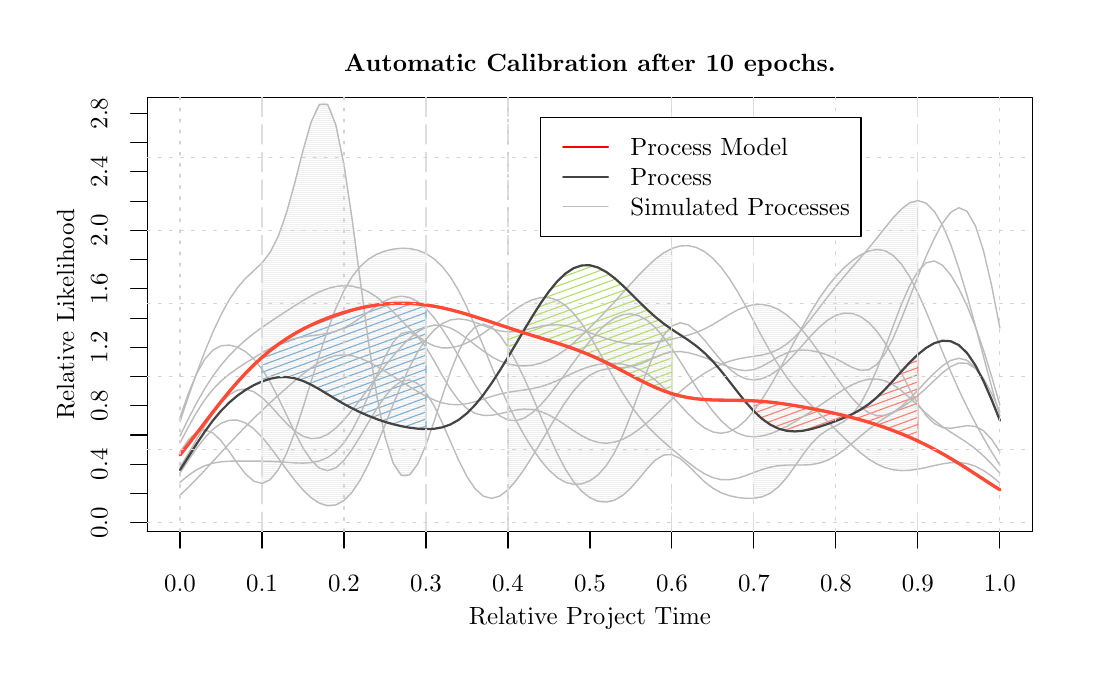
\begin{tikzpicture}[x=1pt,y=1pt]
\definecolor{fillColor}{RGB}{255,255,255}
\path[use as bounding box,fill=fillColor,fill opacity=0.00] (0,0) rectangle (376.36,231.26);
\begin{scope}
\path[clip] ( 43.20, 49.20) rectangle (363.16,206.06);
\definecolor{drawColor}{RGB}{255,74,54}

\path[draw=drawColor,line width= 0.8pt,line join=round,line cap=round] ( 55.05, 76.86) --
	( 58.01, 80.65) --
	( 60.98, 84.53) --
	( 63.94, 88.45) --
	( 66.90, 92.33) --
	( 69.86, 96.11) --
	( 72.83, 99.75) --
	( 75.79,103.19) --
	( 78.75,106.41) --
	( 81.71,109.39) --
	( 84.68,112.12) --
	( 87.64,114.61) --
	( 90.60,116.86) --
	( 93.56,118.88) --
	( 96.53,120.70) --
	( 99.49,122.34) --
	(102.45,123.81) --
	(105.41,125.14) --
	(108.38,126.34) --
	(111.34,127.41) --
	(114.30,128.37) --
	(117.26,129.22) --
	(120.23,129.96) --
	(123.19,130.57) --
	(126.15,131.06) --
	(129.11,131.42) --
	(132.08,131.63) --
	(135.04,131.70) --
	(138.00,131.63) --
	(140.96,131.42) --
	(143.93,131.07) --
	(146.89,130.60) --
	(149.85,130.01) --
	(152.82,129.32) --
	(155.78,128.54) --
	(158.74,127.69) --
	(161.70,126.77) --
	(164.67,125.82) --
	(167.63,124.84) --
	(170.59,123.85) --
	(173.55,122.87) --
	(176.52,121.90) --
	(179.48,120.95) --
	(182.44,120.02) --
	(185.40,119.11) --
	(188.37,118.19) --
	(191.33,117.26) --
	(194.29,116.29) --
	(197.25,115.26) --
	(200.22,114.15) --
	(203.18,112.94) --
	(206.14,111.63) --
	(209.10,110.23) --
	(212.07,108.74) --
	(215.03,107.19) --
	(217.99,105.62) --
	(220.95,104.07) --
	(223.92,102.59) --
	(226.88,101.23) --
	(229.84,100.02) --
	(232.80, 99.00) --
	(235.77, 98.19) --
	(238.73, 97.57) --
	(241.69, 97.14) --
	(244.65, 96.88) --
	(247.62, 96.73) --
	(250.58, 96.67) --
	(253.54, 96.64) --
	(256.51, 96.60) --
	(259.47, 96.54) --
	(262.43, 96.41) --
	(265.39, 96.21) --
	(268.36, 95.93) --
	(271.32, 95.58) --
	(274.28, 95.16) --
	(277.24, 94.69) --
	(280.21, 94.18) --
	(283.17, 93.63) --
	(286.13, 93.05) --
	(289.09, 92.44) --
	(292.06, 91.79) --
	(295.02, 91.10) --
	(297.98, 90.35) --
	(300.94, 89.55) --
	(303.91, 88.69) --
	(306.87, 87.75) --
	(309.83, 86.74) --
	(312.79, 85.65) --
	(315.76, 84.49) --
	(318.72, 83.24) --
	(321.68, 81.90) --
	(324.64, 80.46) --
	(327.61, 78.93) --
	(330.57, 77.31) --
	(333.53, 75.59) --
	(336.49, 73.79) --
	(339.46, 71.92) --
	(342.42, 70.00) --
	(345.38, 68.07) --
	(348.34, 66.15) --
	(351.31, 64.27);
\end{scope}
\begin{scope}
\path[clip] (  0.00,  0.00) rectangle (376.36,231.26);
\definecolor{drawColor}{RGB}{0,0,0}

\path[draw=drawColor,line width= 0.4pt,line join=round,line cap=round] ( 43.20, 49.20) --
	(363.16, 49.20) --
	(363.16,206.06) --
	( 43.20,206.06) --
	( 43.20, 49.20);
\end{scope}
\begin{scope}
\path[clip] (  0.00,  0.00) rectangle (376.36,231.26);
\definecolor{drawColor}{RGB}{0,0,0}

\node[text=drawColor,anchor=base,inner sep=0pt, outer sep=0pt, scale=  0.90] at (203.18,215.56) {\bfseries Automatic Calibration after 10 epochs.};
\end{scope}
\begin{scope}
\path[clip] (  0.00,  0.00) rectangle (376.36,231.26);
\definecolor{drawColor}{RGB}{0,0,0}

\node[text=drawColor,anchor=base,inner sep=0pt, outer sep=0pt, scale=  0.90] at (203.18, 15.60) {Relative Project Time};

\node[text=drawColor,rotate= 90.00,anchor=base,inner sep=0pt, outer sep=0pt, scale=  0.90] at ( 16.80,127.63) {Relative Likelihood};

\path[draw=drawColor,line width= 0.4pt,line join=round,line cap=round] ( 55.05, 49.20) -- (351.31, 49.20);

\path[draw=drawColor,line width= 0.4pt,line join=round,line cap=round] ( 55.05, 49.20) -- ( 55.05, 43.20);

\path[draw=drawColor,line width= 0.4pt,line join=round,line cap=round] ( 84.68, 49.20) -- ( 84.68, 43.20);

\path[draw=drawColor,line width= 0.4pt,line join=round,line cap=round] (114.30, 49.20) -- (114.30, 43.20);

\path[draw=drawColor,line width= 0.4pt,line join=round,line cap=round] (143.93, 49.20) -- (143.93, 43.20);

\path[draw=drawColor,line width= 0.4pt,line join=round,line cap=round] (173.55, 49.20) -- (173.55, 43.20);

\path[draw=drawColor,line width= 0.4pt,line join=round,line cap=round] (203.18, 49.20) -- (203.18, 43.20);

\path[draw=drawColor,line width= 0.4pt,line join=round,line cap=round] (232.80, 49.20) -- (232.80, 43.20);

\path[draw=drawColor,line width= 0.4pt,line join=round,line cap=round] (262.43, 49.20) -- (262.43, 43.20);

\path[draw=drawColor,line width= 0.4pt,line join=round,line cap=round] (292.06, 49.20) -- (292.06, 43.20);

\path[draw=drawColor,line width= 0.4pt,line join=round,line cap=round] (321.68, 49.20) -- (321.68, 43.20);

\path[draw=drawColor,line width= 0.4pt,line join=round,line cap=round] (351.31, 49.20) -- (351.31, 43.20);

\node[text=drawColor,anchor=base,inner sep=0pt, outer sep=0pt, scale=  0.90] at ( 55.05, 27.60) {0.0};

\node[text=drawColor,anchor=base,inner sep=0pt, outer sep=0pt, scale=  0.90] at ( 84.68, 27.60) {0.1};

\node[text=drawColor,anchor=base,inner sep=0pt, outer sep=0pt, scale=  0.90] at (114.30, 27.60) {0.2};

\node[text=drawColor,anchor=base,inner sep=0pt, outer sep=0pt, scale=  0.90] at (143.93, 27.60) {0.3};

\node[text=drawColor,anchor=base,inner sep=0pt, outer sep=0pt, scale=  0.90] at (173.55, 27.60) {0.4};

\node[text=drawColor,anchor=base,inner sep=0pt, outer sep=0pt, scale=  0.90] at (203.18, 27.60) {0.5};

\node[text=drawColor,anchor=base,inner sep=0pt, outer sep=0pt, scale=  0.90] at (232.80, 27.60) {0.6};

\node[text=drawColor,anchor=base,inner sep=0pt, outer sep=0pt, scale=  0.90] at (262.43, 27.60) {0.7};

\node[text=drawColor,anchor=base,inner sep=0pt, outer sep=0pt, scale=  0.90] at (292.06, 27.60) {0.8};

\node[text=drawColor,anchor=base,inner sep=0pt, outer sep=0pt, scale=  0.90] at (321.68, 27.60) {0.9};

\node[text=drawColor,anchor=base,inner sep=0pt, outer sep=0pt, scale=  0.90] at (351.31, 27.60) {1.0};

\path[draw=drawColor,line width= 0.4pt,line join=round,line cap=round] ( 43.20, 52.37) -- ( 43.20,200.25);

\path[draw=drawColor,line width= 0.4pt,line join=round,line cap=round] ( 43.20, 52.37) -- ( 37.20, 52.37);

\path[draw=drawColor,line width= 0.4pt,line join=round,line cap=round] ( 43.20, 62.93) -- ( 37.20, 62.93);

\path[draw=drawColor,line width= 0.4pt,line join=round,line cap=round] ( 43.20, 73.50) -- ( 37.20, 73.50);

\path[draw=drawColor,line width= 0.4pt,line join=round,line cap=round] ( 43.20, 84.06) -- ( 37.20, 84.06);

\path[draw=drawColor,line width= 0.4pt,line join=round,line cap=round] ( 43.20, 94.62) -- ( 37.20, 94.62);

\path[draw=drawColor,line width= 0.4pt,line join=round,line cap=round] ( 43.20,105.19) -- ( 37.20,105.19);

\path[draw=drawColor,line width= 0.4pt,line join=round,line cap=round] ( 43.20,115.75) -- ( 37.20,115.75);

\path[draw=drawColor,line width= 0.4pt,line join=round,line cap=round] ( 43.20,126.31) -- ( 37.20,126.31);

\path[draw=drawColor,line width= 0.4pt,line join=round,line cap=round] ( 43.20,136.87) -- ( 37.20,136.87);

\path[draw=drawColor,line width= 0.4pt,line join=round,line cap=round] ( 43.20,147.44) -- ( 37.20,147.44);

\path[draw=drawColor,line width= 0.4pt,line join=round,line cap=round] ( 43.20,158.00) -- ( 37.20,158.00);

\path[draw=drawColor,line width= 0.4pt,line join=round,line cap=round] ( 43.20,168.56) -- ( 37.20,168.56);

\path[draw=drawColor,line width= 0.4pt,line join=round,line cap=round] ( 43.20,179.13) -- ( 37.20,179.13);

\path[draw=drawColor,line width= 0.4pt,line join=round,line cap=round] ( 43.20,189.69) -- ( 37.20,189.69);

\path[draw=drawColor,line width= 0.4pt,line join=round,line cap=round] ( 43.20,200.25) -- ( 37.20,200.25);

\node[text=drawColor,rotate= 90.00,anchor=base,inner sep=0pt, outer sep=0pt, scale=  0.90] at ( 28.80, 52.37) {0.0};

\node[text=drawColor,rotate= 90.00,anchor=base,inner sep=0pt, outer sep=0pt, scale=  0.90] at ( 28.80, 73.50) {0.4};

\node[text=drawColor,rotate= 90.00,anchor=base,inner sep=0pt, outer sep=0pt, scale=  0.90] at ( 28.80, 94.62) {0.8};

\node[text=drawColor,rotate= 90.00,anchor=base,inner sep=0pt, outer sep=0pt, scale=  0.90] at ( 28.80,115.75) {1.2};

\node[text=drawColor,rotate= 90.00,anchor=base,inner sep=0pt, outer sep=0pt, scale=  0.90] at ( 28.80,136.87) {1.6};

\node[text=drawColor,rotate= 90.00,anchor=base,inner sep=0pt, outer sep=0pt, scale=  0.90] at ( 28.80,158.00) {2.0};

\node[text=drawColor,rotate= 90.00,anchor=base,inner sep=0pt, outer sep=0pt, scale=  0.90] at ( 28.80,179.13) {2.4};

\node[text=drawColor,rotate= 90.00,anchor=base,inner sep=0pt, outer sep=0pt, scale=  0.90] at ( 28.80,200.25) {2.8};
\end{scope}
\begin{scope}
\path[clip] ( 43.20, 49.20) rectangle (363.16,206.06);
\definecolor{drawColor}{RGB}{238,238,238}

\path[draw=drawColor,draw opacity=0.97,line width= 0.4pt,line join=round,line cap=round] (321.45, 82.00) -- (321.68, 82.00);

\path[draw=drawColor,draw opacity=0.97,line width= 0.4pt,line join=round,line cap=round] (319.86, 82.72) -- (321.68, 82.72);

\path[draw=drawColor,draw opacity=0.97,line width= 0.4pt,line join=round,line cap=round] (262.43, 83.45) -- (262.88, 83.45);

\path[draw=drawColor,draw opacity=0.97,line width= 0.4pt,line join=round,line cap=round] (318.22, 83.45) -- (321.68, 83.45);

\path[draw=drawColor,draw opacity=0.97,line width= 0.4pt,line join=round,line cap=round] (262.43, 84.17) -- (267.19, 84.17);

\path[draw=drawColor,draw opacity=0.97,line width= 0.4pt,line join=round,line cap=round] (316.53, 84.17) -- (321.68, 84.17);

\path[draw=drawColor,draw opacity=0.97,line width= 0.4pt,line join=round,line cap=round] (262.43, 84.89) -- (269.29, 84.89);

\path[draw=drawColor,draw opacity=0.97,line width= 0.4pt,line join=round,line cap=round] (314.74, 84.89) -- (321.68, 84.89);

\path[draw=drawColor,draw opacity=0.97,line width= 0.4pt,line join=round,line cap=round] (262.43, 85.61) -- (271.03, 85.61);

\path[draw=drawColor,draw opacity=0.97,line width= 0.4pt,line join=round,line cap=round] (312.88, 85.61) -- (321.68, 85.61);

\path[draw=drawColor,draw opacity=0.97,line width= 0.4pt,line join=round,line cap=round] (262.43, 86.34) -- (272.61, 86.34);

\path[draw=drawColor,draw opacity=0.97,line width= 0.4pt,line join=round,line cap=round] (310.94, 86.34) -- (321.68, 86.34);

\path[draw=drawColor,draw opacity=0.97,line width= 0.4pt,line join=round,line cap=round] (262.43, 87.06) -- (274.01, 87.06);

\path[draw=drawColor,draw opacity=0.97,line width= 0.4pt,line join=round,line cap=round] (308.91, 87.06) -- (321.68, 87.06);

\path[draw=drawColor,draw opacity=0.97,line width= 0.4pt,line join=round,line cap=round] (262.43, 87.78) -- (275.35, 87.78);

\path[draw=drawColor,draw opacity=0.97,line width= 0.4pt,line join=round,line cap=round] (306.77, 87.78) -- (321.68, 87.78);

\path[draw=drawColor,draw opacity=0.97,line width= 0.4pt,line join=round,line cap=round] (262.43, 88.50) -- (276.61, 88.50);

\path[draw=drawColor,draw opacity=0.97,line width= 0.4pt,line join=round,line cap=round] (304.50, 88.50) -- (321.68, 88.50);

\path[draw=drawColor,draw opacity=0.97,line width= 0.4pt,line join=round,line cap=round] (262.43, 89.23) -- (277.83, 89.23);

\path[draw=drawColor,draw opacity=0.97,line width= 0.4pt,line join=round,line cap=round] (302.08, 89.23) -- (321.68, 89.23);

\path[draw=drawColor,draw opacity=0.97,line width= 0.4pt,line join=round,line cap=round] (262.43, 89.95) -- (279.01, 89.95);

\path[draw=drawColor,draw opacity=0.97,line width= 0.4pt,line join=round,line cap=round] (299.51, 89.95) -- (321.68, 89.95);

\path[draw=drawColor,draw opacity=0.97,line width= 0.4pt,line join=round,line cap=round] (262.43, 90.67) -- (280.16, 90.67);

\path[draw=drawColor,draw opacity=0.97,line width= 0.4pt,line join=round,line cap=round] (296.74, 90.67) -- (321.68, 90.67);

\path[draw=drawColor,draw opacity=0.97,line width= 0.4pt,line join=round,line cap=round] (262.43, 91.39) -- (281.27, 91.39);

\path[draw=drawColor,draw opacity=0.97,line width= 0.4pt,line join=round,line cap=round] (293.76, 91.39) -- (321.68, 91.39);

\path[draw=drawColor,draw opacity=0.97,line width= 0.4pt,line join=round,line cap=round] (262.43, 92.12) -- (282.42, 92.12);

\path[draw=drawColor,draw opacity=0.97,line width= 0.4pt,line join=round,line cap=round] (290.57, 92.12) -- (321.68, 92.12);

\path[draw=drawColor,draw opacity=0.97,line width= 0.4pt,line join=round,line cap=round] (262.43, 92.84) -- (283.73, 92.84);

\path[draw=drawColor,draw opacity=0.97,line width= 0.4pt,line join=round,line cap=round] (287.18, 92.84) -- (321.68, 92.84);

\path[draw=drawColor,draw opacity=0.97,line width= 0.4pt,line join=round,line cap=round] (262.43, 93.56) -- (321.68, 93.56);

\path[draw=drawColor,draw opacity=0.97,line width= 0.4pt,line join=round,line cap=round] (262.43, 94.29) -- (279.62, 94.29);

\path[draw=drawColor,draw opacity=0.97,line width= 0.4pt,line join=round,line cap=round] (285.59, 94.29) -- (321.68, 94.29);

\path[draw=drawColor,draw opacity=0.97,line width= 0.4pt,line join=round,line cap=round] (262.43, 95.01) -- (275.27, 95.01);

\path[draw=drawColor,draw opacity=0.97,line width= 0.4pt,line join=round,line cap=round] (286.64, 95.01) -- (321.35, 95.01);

\path[draw=drawColor,draw opacity=0.97,line width= 0.4pt,line join=round,line cap=round] (262.43, 95.73) -- (270.07, 95.73);

\path[draw=drawColor,draw opacity=0.97,line width= 0.4pt,line join=round,line cap=round] (287.69, 95.73) -- (320.59, 95.73);

\path[draw=drawColor,draw opacity=0.97,line width= 0.4pt,line join=round,line cap=round] (288.74, 96.45) -- (319.82, 96.45);

\path[draw=drawColor,draw opacity=0.97,line width= 0.4pt,line join=round,line cap=round] (289.80, 97.18) -- (319.05, 97.18);

\path[draw=drawColor,draw opacity=0.97,line width= 0.4pt,line join=round,line cap=round] (290.87, 97.90) -- (318.25, 97.90);

\path[draw=drawColor,draw opacity=0.97,line width= 0.4pt,line join=round,line cap=round] (291.94, 98.62) -- (317.44, 98.62);

\path[draw=drawColor,draw opacity=0.97,line width= 0.4pt,line join=round,line cap=round] (293.06, 99.34) -- (316.62, 99.34);

\path[draw=drawColor,draw opacity=0.97,line width= 0.4pt,line join=round,line cap=round] (294.18,100.07) -- (315.70,100.07);

\path[draw=drawColor,draw opacity=0.97,line width= 0.4pt,line join=round,line cap=round] (295.39,100.79) -- (314.78,100.79);

\path[draw=drawColor,draw opacity=0.97,line width= 0.4pt,line join=round,line cap=round] (296.64,101.51) -- (313.75,101.51);

\path[draw=drawColor,draw opacity=0.97,line width= 0.4pt,line join=round,line cap=round] (298.05,102.24) -- (312.59,102.24);

\path[draw=drawColor,draw opacity=0.97,line width= 0.4pt,line join=round,line cap=round] (299.55,102.96) -- (311.26,102.96);

\path[draw=drawColor,draw opacity=0.97,line width= 0.4pt,line join=round,line cap=round] (301.56,103.68) -- (309.56,103.68);

\path[draw=drawColor,draw opacity=0.97,line width= 0.4pt,line join=round,line cap=round] (262.43, 96.41) --
	(264.90, 96.24) --
	(267.37, 96.03) --
	(269.84, 95.76) --
	(272.31, 95.45) --
	(274.77, 95.09) --
	(277.24, 94.69) --
	(279.71, 94.27) --
	(282.18, 93.82) --
	(284.65, 93.64) --
	(287.12, 95.34) --
	(289.59, 97.03) --
	(292.06, 98.70) --
	(294.52,100.29) --
	(296.99,101.72) --
	(299.46,102.93) --
	(301.93,103.82) --
	(304.40,104.30) --
	(306.87,104.30) --
	(309.34,103.78) --
	(311.81,102.72) --
	(314.28,101.18) --
	(316.74, 99.24) --
	(319.21, 97.03) --
	(321.68, 94.69) --
	(321.68, 81.90) --
	(319.21, 83.02) --
	(316.74, 84.08) --
	(314.28, 85.08) --
	(311.81, 86.03) --
	(309.34, 86.91) --
	(306.87, 87.75) --
	(304.40, 88.54) --
	(301.93, 89.27) --
	(299.46, 89.96) --
	(296.99, 90.61) --
	(294.52, 91.22) --
	(292.06, 91.79) --
	(289.59, 92.33) --
	(287.12, 92.85) --
	(284.65, 93.35) --
	(282.18, 91.98) --
	(279.71, 90.38) --
	(277.24, 88.87) --
	(274.77, 87.45) --
	(272.31, 86.18) --
	(269.84, 85.08) --
	(267.37, 84.21) --
	(264.90, 83.63) --
	(262.43, 83.40) --
	(262.43, 96.41);

\path[draw=drawColor,draw opacity=0.97,line width= 0.4pt,line join=round,line cap=round] ( 84.68,112.35) -- ( 84.95,112.35);

\path[draw=drawColor,draw opacity=0.97,line width= 0.4pt,line join=round,line cap=round] ( 84.68,113.08) -- ( 85.80,113.08);

\path[draw=drawColor,draw opacity=0.97,line width= 0.4pt,line join=round,line cap=round] ( 84.79,113.80) -- ( 86.66,113.80);

\path[draw=drawColor,draw opacity=0.97,line width= 0.4pt,line join=round,line cap=round] ( 86.05,114.52) -- ( 87.54,114.52);

\path[draw=drawColor,draw opacity=0.97,line width= 0.4pt,line join=round,line cap=round] ( 87.33,115.24) -- ( 88.47,115.24);

\path[draw=drawColor,draw opacity=0.97,line width= 0.4pt,line join=round,line cap=round] ( 88.73,115.97) -- ( 89.40,115.97);

\path[draw=drawColor,draw opacity=0.97,line width= 0.4pt,line join=round,line cap=round] ( 90.06,116.69) -- ( 90.61,116.69);

\path[draw=drawColor,draw opacity=0.97,line width= 0.4pt,line join=round,line cap=round] ( 91.27,117.41) -- ( 91.89,117.41);

\path[draw=drawColor,draw opacity=0.97,line width= 0.4pt,line join=round,line cap=round] ( 92.45,118.13) -- ( 93.82,118.13);

\path[draw=drawColor,draw opacity=0.97,line width= 0.4pt,line join=round,line cap=round] ( 93.55,118.86) -- ( 96.29,118.86);

\path[draw=drawColor,draw opacity=0.97,line width= 0.4pt,line join=round,line cap=round] ( 94.67,119.58) -- ( 99.91,119.58);

\path[draw=drawColor,draw opacity=0.97,line width= 0.4pt,line join=round,line cap=round] ( 95.87,120.30) -- (105.33,120.30);

\path[draw=drawColor,draw opacity=0.97,line width= 0.4pt,line join=round,line cap=round] ( 97.09,121.03) -- (109.28,121.03);

\path[draw=drawColor,draw opacity=0.97,line width= 0.4pt,line join=round,line cap=round] ( 98.41,121.75) -- (111.71,121.75);

\path[draw=drawColor,draw opacity=0.97,line width= 0.4pt,line join=round,line cap=round] ( 99.75,122.47) -- (113.49,122.47);

\path[draw=drawColor,draw opacity=0.97,line width= 0.4pt,line join=round,line cap=round] (101.19,123.19) -- (115.02,123.19);

\path[draw=drawColor,draw opacity=0.97,line width= 0.4pt,line join=round,line cap=round] (102.70,123.92) -- (116.37,123.92);

\path[draw=drawColor,draw opacity=0.97,line width= 0.4pt,line join=round,line cap=round] (104.27,124.64) -- (117.57,124.64);

\path[draw=drawColor,draw opacity=0.97,line width= 0.4pt,line join=round,line cap=round] (105.97,125.36) -- (118.69,125.36);

\path[draw=drawColor,draw opacity=0.97,line width= 0.4pt,line join=round,line cap=round] (107.75,126.08) -- (119.76,126.08);

\path[draw=drawColor,draw opacity=0.97,line width= 0.4pt,line join=round,line cap=round] (109.65,126.81) -- (120.77,126.81);

\path[draw=drawColor,draw opacity=0.97,line width= 0.4pt,line join=round,line cap=round] (111.69,127.53) -- (121.78,127.53);

\path[draw=drawColor,draw opacity=0.97,line width= 0.4pt,line join=round,line cap=round] (113.92,128.25) -- (122.75,128.25);

\path[draw=drawColor,draw opacity=0.97,line width= 0.4pt,line join=round,line cap=round] (116.37,128.98) -- (123.73,128.98);

\path[draw=drawColor,draw opacity=0.97,line width= 0.4pt,line join=round,line cap=round] (119.12,129.70) -- (124.73,129.70);

\path[draw=drawColor,draw opacity=0.97,line width= 0.4pt,line join=round,line cap=round] (122.44,130.42) -- (125.76,130.42);

\path[draw=drawColor,draw opacity=0.97,line width= 0.4pt,line join=round,line cap=round] (142.94,130.42) -- (143.93,130.42);

\path[draw=drawColor,draw opacity=0.97,line width= 0.4pt,line join=round,line cap=round] (126.67,131.14) -- (127.30,131.14);

\path[draw=drawColor,draw opacity=0.97,line width= 0.4pt,line join=round,line cap=round] (141.81,131.14) -- (143.72,131.14);

\path[draw=drawColor,draw opacity=0.97,line width= 0.4pt,line join=round,line cap=round] (127.94,131.87) -- (141.57,131.87);

\path[draw=drawColor,draw opacity=0.97,line width= 0.4pt,line join=round,line cap=round] (129.23,132.59) -- (140.29,132.59);

\path[draw=drawColor,draw opacity=0.97,line width= 0.4pt,line join=round,line cap=round] (130.87,133.31) -- (139.06,133.31);

\path[draw=drawColor,draw opacity=0.97,line width= 0.4pt,line join=round,line cap=round] (133.39,134.03) -- (136.77,134.03);

\path[draw=drawColor,draw opacity=0.97,line width= 0.4pt,line join=round,line cap=round] ( 84.68,113.74) --
	( 87.14,115.15) --
	( 89.61,116.42) --
	( 92.08,117.90) --
	( 94.55,119.51) --
	( 97.02,120.99) --
	( 99.49,122.34) --
	(101.96,123.58) --
	(104.43,124.71) --
	(106.90,125.75) --
	(109.36,126.71) --
	(111.83,127.58) --
	(114.30,128.37) --
	(116.77,129.09) --
	(119.24,129.73) --
	(121.71,130.28) --
	(124.18,130.75) --
	(126.65,131.13) --
	(129.11,132.54) --
	(131.58,133.63) --
	(134.05,134.18) --
	(136.52,134.11) --
	(138.99,133.35) --
	(141.46,131.90) --
	(143.93,131.07) --
	(143.93,129.78) --
	(141.46,131.37) --
	(138.99,131.57) --
	(136.52,131.68) --
	(134.05,131.69) --
	(131.58,131.60) --
	(129.11,131.42) --
	(126.65,131.05) --
	(124.18,129.31) --
	(121.71,127.48) --
	(119.24,125.71) --
	(116.77,124.13) --
	(114.30,122.81) --
	(111.83,121.78) --
	(109.36,121.04) --
	(106.90,120.53) --
	(104.43,120.17) --
	(101.96,119.87) --
	( 99.49,119.52) --
	( 97.02,119.05) --
	( 94.55,118.39) --
	( 92.08,117.52) --
	( 89.61,116.13) --
	( 87.14,114.21) --
	( 84.68,112.12) --
	( 84.68,113.74);

\path[draw=drawColor,draw opacity=0.97,line width= 0.4pt,line join=round,line cap=round] (175.84, 89.23) -- (176.12, 89.23);

\path[draw=drawColor,draw opacity=0.97,line width= 0.4pt,line join=round,line cap=round] (173.55, 89.95) -- (178.84, 89.95);

\path[draw=drawColor,draw opacity=0.97,line width= 0.4pt,line join=round,line cap=round] (173.55, 90.67) -- (180.20, 90.67);

\path[draw=drawColor,draw opacity=0.97,line width= 0.4pt,line join=round,line cap=round] (173.55, 91.39) -- (181.36, 91.39);

\path[draw=drawColor,draw opacity=0.97,line width= 0.4pt,line join=round,line cap=round] (173.55, 92.12) -- (182.27, 92.12);

\path[draw=drawColor,draw opacity=0.97,line width= 0.4pt,line join=round,line cap=round] (173.55, 92.84) -- (183.18, 92.84);

\path[draw=drawColor,draw opacity=0.97,line width= 0.4pt,line join=round,line cap=round] (173.55, 93.56) -- (183.95, 93.56);

\path[draw=drawColor,draw opacity=0.97,line width= 0.4pt,line join=round,line cap=round] (173.55, 94.29) -- (184.67, 94.29);

\path[draw=drawColor,draw opacity=0.97,line width= 0.4pt,line join=round,line cap=round] (173.55, 95.01) -- (185.39, 95.01);

\path[draw=drawColor,draw opacity=0.97,line width= 0.4pt,line join=round,line cap=round] (173.55, 95.73) -- (186.08, 95.73);

\path[draw=drawColor,draw opacity=0.97,line width= 0.4pt,line join=round,line cap=round] (173.55, 96.45) -- (186.70, 96.45);

\path[draw=drawColor,draw opacity=0.97,line width= 0.4pt,line join=round,line cap=round] (173.55, 97.18) -- (187.32, 97.18);

\path[draw=drawColor,draw opacity=0.97,line width= 0.4pt,line join=round,line cap=round] (173.55, 97.90) -- (187.94, 97.90);

\path[draw=drawColor,draw opacity=0.97,line width= 0.4pt,line join=round,line cap=round] (173.55, 98.62) -- (188.55, 98.62);

\path[draw=drawColor,draw opacity=0.97,line width= 0.4pt,line join=round,line cap=round] (173.55, 99.34) -- (189.11, 99.34);

\path[draw=drawColor,draw opacity=0.97,line width= 0.4pt,line join=round,line cap=round] (231.80, 99.34) -- (232.80, 99.34);

\path[draw=drawColor,draw opacity=0.97,line width= 0.4pt,line join=round,line cap=round] (173.55,100.07) -- (189.68,100.07);

\path[draw=drawColor,draw opacity=0.97,line width= 0.4pt,line join=round,line cap=round] (229.75,100.07) -- (232.80,100.07);

\path[draw=drawColor,draw opacity=0.97,line width= 0.4pt,line join=round,line cap=round] (173.55,100.79) -- (190.25,100.79);

\path[draw=drawColor,draw opacity=0.97,line width= 0.4pt,line join=round,line cap=round] (227.91,100.79) -- (232.80,100.79);

\path[draw=drawColor,draw opacity=0.97,line width= 0.4pt,line join=round,line cap=round] (173.55,101.51) -- (190.81,101.51);

\path[draw=drawColor,draw opacity=0.97,line width= 0.4pt,line join=round,line cap=round] (226.26,101.51) -- (232.80,101.51);

\path[draw=drawColor,draw opacity=0.97,line width= 0.4pt,line join=round,line cap=round] (173.55,102.24) -- (191.35,102.24);

\path[draw=drawColor,draw opacity=0.97,line width= 0.4pt,line join=round,line cap=round] (224.68,102.24) -- (232.80,102.24);

\path[draw=drawColor,draw opacity=0.97,line width= 0.4pt,line join=round,line cap=round] (173.55,102.96) -- (191.89,102.96);

\path[draw=drawColor,draw opacity=0.97,line width= 0.4pt,line join=round,line cap=round] (223.17,102.96) -- (232.80,102.96);

\path[draw=drawColor,draw opacity=0.97,line width= 0.4pt,line join=round,line cap=round] (173.55,103.68) -- (192.42,103.68);

\path[draw=drawColor,draw opacity=0.97,line width= 0.4pt,line join=round,line cap=round] (221.73,103.68) -- (232.80,103.68);

\path[draw=drawColor,draw opacity=0.97,line width= 0.4pt,line join=round,line cap=round] (173.55,104.40) -- (192.96,104.40);

\path[draw=drawColor,draw opacity=0.97,line width= 0.4pt,line join=round,line cap=round] (220.31,104.40) -- (232.80,104.40);

\path[draw=drawColor,draw opacity=0.97,line width= 0.4pt,line join=round,line cap=round] (173.55,105.13) -- (193.49,105.13);

\path[draw=drawColor,draw opacity=0.97,line width= 0.4pt,line join=round,line cap=round] (218.93,105.13) -- (232.80,105.13);

\path[draw=drawColor,draw opacity=0.97,line width= 0.4pt,line join=round,line cap=round] (173.55,105.85) -- (194.02,105.85);

\path[draw=drawColor,draw opacity=0.97,line width= 0.4pt,line join=round,line cap=round] (217.55,105.85) -- (232.80,105.85);

\path[draw=drawColor,draw opacity=0.97,line width= 0.4pt,line join=round,line cap=round] (173.55,106.57) -- (194.54,106.57);

\path[draw=drawColor,draw opacity=0.97,line width= 0.4pt,line join=round,line cap=round] (216.19,106.57) -- (232.80,106.57);

\path[draw=drawColor,draw opacity=0.97,line width= 0.4pt,line join=round,line cap=round] (173.55,107.29) -- (195.07,107.29);

\path[draw=drawColor,draw opacity=0.97,line width= 0.4pt,line join=round,line cap=round] (214.82,107.29) -- (232.80,107.29);

\path[draw=drawColor,draw opacity=0.97,line width= 0.4pt,line join=round,line cap=round] (173.55,108.02) -- (195.59,108.02);

\path[draw=drawColor,draw opacity=0.97,line width= 0.4pt,line join=round,line cap=round] (213.45,108.02) -- (232.80,108.02);

\path[draw=drawColor,draw opacity=0.97,line width= 0.4pt,line join=round,line cap=round] (173.55,108.74) -- (196.12,108.74);

\path[draw=drawColor,draw opacity=0.97,line width= 0.4pt,line join=round,line cap=round] (212.05,108.74) -- (232.80,108.74);

\path[draw=drawColor,draw opacity=0.97,line width= 0.4pt,line join=round,line cap=round] (173.55,109.46) -- (196.64,109.46);

\path[draw=drawColor,draw opacity=0.97,line width= 0.4pt,line join=round,line cap=round] (210.64,109.46) -- (232.80,109.46);

\path[draw=drawColor,draw opacity=0.97,line width= 0.4pt,line join=round,line cap=round] (173.55,110.18) -- (197.17,110.18);

\path[draw=drawColor,draw opacity=0.97,line width= 0.4pt,line join=round,line cap=round] (209.18,110.18) -- (232.80,110.18);

\path[draw=drawColor,draw opacity=0.97,line width= 0.4pt,line join=round,line cap=round] (173.55,110.91) -- (197.70,110.91);

\path[draw=drawColor,draw opacity=0.97,line width= 0.4pt,line join=round,line cap=round] (207.69,110.91) -- (232.80,110.91);

\path[draw=drawColor,draw opacity=0.97,line width= 0.4pt,line join=round,line cap=round] (173.55,111.63) -- (198.22,111.63);

\path[draw=drawColor,draw opacity=0.97,line width= 0.4pt,line join=round,line cap=round] (206.14,111.63) -- (232.80,111.63);

\path[draw=drawColor,draw opacity=0.97,line width= 0.4pt,line join=round,line cap=round] (173.55,112.35) -- (198.99,112.35);

\path[draw=drawColor,draw opacity=0.97,line width= 0.4pt,line join=round,line cap=round] (204.52,112.35) -- (232.80,112.35);

\path[draw=drawColor,draw opacity=0.97,line width= 0.4pt,line join=round,line cap=round] (173.55,113.08) -- (199.77,113.08);

\path[draw=drawColor,draw opacity=0.97,line width= 0.4pt,line join=round,line cap=round] (202.85,113.08) -- (232.80,113.08);

\path[draw=drawColor,draw opacity=0.97,line width= 0.4pt,line join=round,line cap=round] (173.55,113.80) -- (200.54,113.80);

\path[draw=drawColor,draw opacity=0.97,line width= 0.4pt,line join=round,line cap=round] (201.09,113.80) -- (232.80,113.80);

\path[draw=drawColor,draw opacity=0.97,line width= 0.4pt,line join=round,line cap=round] (173.55,114.52) -- (232.80,114.52);

\path[draw=drawColor,draw opacity=0.97,line width= 0.4pt,line join=round,line cap=round] (173.55,115.24) -- (197.28,115.24);

\path[draw=drawColor,draw opacity=0.97,line width= 0.4pt,line join=round,line cap=round] (200.94,115.24) -- (232.80,115.24);

\path[draw=drawColor,draw opacity=0.97,line width= 0.4pt,line join=round,line cap=round] (173.55,115.97) -- (195.23,115.97);

\path[draw=drawColor,draw opacity=0.97,line width= 0.4pt,line join=round,line cap=round] (201.52,115.97) -- (232.29,115.97);

\path[draw=drawColor,draw opacity=0.97,line width= 0.4pt,line join=round,line cap=round] (173.55,116.69) -- (193.09,116.69);

\path[draw=drawColor,draw opacity=0.97,line width= 0.4pt,line join=round,line cap=round] (202.09,116.69) -- (231.77,116.69);

\path[draw=drawColor,draw opacity=0.97,line width= 0.4pt,line join=round,line cap=round] (173.55,117.41) -- (190.85,117.41);

\path[draw=drawColor,draw opacity=0.97,line width= 0.4pt,line join=round,line cap=round] (202.66,117.41) -- (231.26,117.41);

\path[draw=drawColor,draw opacity=0.97,line width= 0.4pt,line join=round,line cap=round] (173.55,118.13) -- (188.55,118.13);

\path[draw=drawColor,draw opacity=0.97,line width= 0.4pt,line join=round,line cap=round] (203.24,118.13) -- (230.74,118.13);

\path[draw=drawColor,draw opacity=0.97,line width= 0.4pt,line join=round,line cap=round] (173.55,118.86) -- (186.21,118.86);

\path[draw=drawColor,draw opacity=0.97,line width= 0.4pt,line join=round,line cap=round] (203.87,118.86) -- (230.21,118.86);

\path[draw=drawColor,draw opacity=0.97,line width= 0.4pt,line join=round,line cap=round] (173.55,119.58) -- (183.87,119.58);

\path[draw=drawColor,draw opacity=0.97,line width= 0.4pt,line join=round,line cap=round] (204.50,119.58) -- (229.62,119.58);

\path[draw=drawColor,draw opacity=0.97,line width= 0.4pt,line join=round,line cap=round] (173.55,120.30) -- (181.55,120.30);

\path[draw=drawColor,draw opacity=0.97,line width= 0.4pt,line join=round,line cap=round] (205.13,120.30) -- (229.03,120.30);

\path[draw=drawColor,draw opacity=0.97,line width= 0.4pt,line join=round,line cap=round] (173.55,121.03) -- (179.25,121.03);

\path[draw=drawColor,draw opacity=0.97,line width= 0.4pt,line join=round,line cap=round] (205.78,121.03) -- (228.44,121.03);

\path[draw=drawColor,draw opacity=0.97,line width= 0.4pt,line join=round,line cap=round] (173.55,121.75) -- (176.99,121.75);

\path[draw=drawColor,draw opacity=0.97,line width= 0.4pt,line join=round,line cap=round] (206.50,121.75) -- (227.85,121.75);

\path[draw=drawColor,draw opacity=0.97,line width= 0.4pt,line join=round,line cap=round] (173.55,122.47) -- (174.77,122.47);

\path[draw=drawColor,draw opacity=0.97,line width= 0.4pt,line join=round,line cap=round] (207.23,122.47) -- (227.14,122.47);

\path[draw=drawColor,draw opacity=0.97,line width= 0.4pt,line join=round,line cap=round] (207.95,123.19) -- (226.42,123.19);

\path[draw=drawColor,draw opacity=0.97,line width= 0.4pt,line join=round,line cap=round] (208.80,123.92) -- (225.71,123.92);

\path[draw=drawColor,draw opacity=0.97,line width= 0.4pt,line join=round,line cap=round] (209.69,124.64) -- (224.86,124.64);

\path[draw=drawColor,draw opacity=0.97,line width= 0.4pt,line join=round,line cap=round] (210.59,125.36) -- (223.91,125.36);

\path[draw=drawColor,draw opacity=0.97,line width= 0.4pt,line join=round,line cap=round] (211.81,126.08) -- (222.96,126.08);

\path[draw=drawColor,draw opacity=0.97,line width= 0.4pt,line join=round,line cap=round] (213.04,126.81) -- (221.51,126.81);

\path[draw=drawColor,draw opacity=0.97,line width= 0.4pt,line join=round,line cap=round] (215.14,127.53) -- (219.46,127.53);

\path[draw=drawColor,draw opacity=0.97,line width= 0.4pt,line join=round,line cap=round] (173.55,122.87) --
	(176.02,122.06) --
	(178.49,121.27) --
	(180.96,120.49) --
	(183.43,119.72) --
	(185.90,118.96) --
	(188.37,118.19) --
	(190.83,117.42) --
	(193.30,116.62) --
	(195.77,115.78) --
	(198.24,114.90) --
	(200.71,114.95) --
	(203.18,118.06) --
	(205.65,120.89) --
	(208.12,123.36) --
	(210.59,125.36) --
	(213.05,126.82) --
	(215.52,127.66) --
	(217.99,127.84) --
	(220.46,127.32) --
	(222.93,126.11) --
	(225.40,124.23) --
	(227.87,121.73) --
	(230.34,118.70) --
	(232.80,115.24) --
	(232.80, 99.00) --
	(230.34, 99.84) --
	(227.87,100.81) --
	(225.40,101.89) --
	(222.93,103.07) --
	(220.46,104.32) --
	(217.99,105.62) --
	(215.52,106.93) --
	(213.05,108.22) --
	(210.59,109.49) --
	(208.12,110.71) --
	(205.65,111.86) --
	(203.18,112.94) --
	(200.71,113.95) --
	(198.24,111.65) --
	(195.77,108.26) --
	(193.30,104.86) --
	(190.83,101.54) --
	(188.37, 98.39) --
	(185.90, 95.52) --
	(183.43, 93.04) --
	(180.96, 91.08) --
	(178.49, 89.76) --
	(176.02, 89.21) --
	(173.55, 89.49) --
	(173.55,122.87);

\path[draw=drawColor,draw opacity=0.97,line width= 0.4pt,line join=round,line cap=round] (321.45, 82.00) -- (321.68, 82.00);

\path[draw=drawColor,draw opacity=0.97,line width= 0.4pt,line join=round,line cap=round] (319.86, 82.72) -- (321.68, 82.72);

\path[draw=drawColor,draw opacity=0.97,line width= 0.4pt,line join=round,line cap=round] (318.22, 83.45) -- (321.68, 83.45);

\path[draw=drawColor,draw opacity=0.97,line width= 0.4pt,line join=round,line cap=round] (316.53, 84.17) -- (321.68, 84.17);

\path[draw=drawColor,draw opacity=0.97,line width= 0.4pt,line join=round,line cap=round] (314.74, 84.89) -- (321.68, 84.89);

\path[draw=drawColor,draw opacity=0.97,line width= 0.4pt,line join=round,line cap=round] (312.88, 85.61) -- (321.68, 85.61);

\path[draw=drawColor,draw opacity=0.97,line width= 0.4pt,line join=round,line cap=round] (310.94, 86.34) -- (321.68, 86.34);

\path[draw=drawColor,draw opacity=0.97,line width= 0.4pt,line join=round,line cap=round] (308.91, 87.06) -- (321.68, 87.06);

\path[draw=drawColor,draw opacity=0.97,line width= 0.4pt,line join=round,line cap=round] (306.77, 87.78) -- (321.68, 87.78);

\path[draw=drawColor,draw opacity=0.97,line width= 0.4pt,line join=round,line cap=round] (304.50, 88.50) -- (321.68, 88.50);

\path[draw=drawColor,draw opacity=0.97,line width= 0.4pt,line join=round,line cap=round] (302.08, 89.23) -- (321.68, 89.23);

\path[draw=drawColor,draw opacity=0.97,line width= 0.4pt,line join=round,line cap=round] (299.51, 89.95) -- (321.68, 89.95);

\path[draw=drawColor,draw opacity=0.97,line width= 0.4pt,line join=round,line cap=round] (296.74, 90.67) -- (321.68, 90.67);

\path[draw=drawColor,draw opacity=0.97,line width= 0.4pt,line join=round,line cap=round] (293.76, 91.39) -- (321.68, 91.39);

\path[draw=drawColor,draw opacity=0.97,line width= 0.4pt,line join=round,line cap=round] (290.57, 92.12) -- (321.68, 92.12);

\path[draw=drawColor,draw opacity=0.97,line width= 0.4pt,line join=round,line cap=round] (287.18, 92.84) -- (321.68, 92.84);

\path[draw=drawColor,draw opacity=0.97,line width= 0.4pt,line join=round,line cap=round] (283.52, 93.56) -- (321.68, 93.56);

\path[draw=drawColor,draw opacity=0.97,line width= 0.4pt,line join=round,line cap=round] (279.62, 94.29) -- (321.68, 94.29);

\path[draw=drawColor,draw opacity=0.97,line width= 0.4pt,line join=round,line cap=round] (275.27, 95.01) -- (321.68, 95.01);

\path[draw=drawColor,draw opacity=0.97,line width= 0.4pt,line join=round,line cap=round] (270.07, 95.73) -- (321.46, 95.73);

\path[draw=drawColor,draw opacity=0.97,line width= 0.4pt,line join=round,line cap=round] (262.43, 96.45) -- (321.05, 96.45);

\path[draw=drawColor,draw opacity=0.97,line width= 0.4pt,line join=round,line cap=round] (262.43, 97.18) -- (320.64, 97.18);

\path[draw=drawColor,draw opacity=0.97,line width= 0.4pt,line join=round,line cap=round] (262.43, 97.90) -- (320.23, 97.90);

\path[draw=drawColor,draw opacity=0.97,line width= 0.4pt,line join=round,line cap=round] (262.43, 98.62) -- (319.82, 98.62);

\path[draw=drawColor,draw opacity=0.97,line width= 0.4pt,line join=round,line cap=round] (262.43, 99.34) -- (319.40, 99.34);

\path[draw=drawColor,draw opacity=0.97,line width= 0.4pt,line join=round,line cap=round] (262.43,100.07) -- (319.01,100.07);

\path[draw=drawColor,draw opacity=0.97,line width= 0.4pt,line join=round,line cap=round] (262.43,100.79) -- (318.64,100.79);

\path[draw=drawColor,draw opacity=0.97,line width= 0.4pt,line join=round,line cap=round] (262.43,101.51) -- (318.27,101.51);

\path[draw=drawColor,draw opacity=0.97,line width= 0.4pt,line join=round,line cap=round] (262.43,102.24) -- (317.89,102.24);

\path[draw=drawColor,draw opacity=0.97,line width= 0.4pt,line join=round,line cap=round] (262.43,102.96) -- (317.52,102.96);

\path[draw=drawColor,draw opacity=0.97,line width= 0.4pt,line join=round,line cap=round] (262.43,103.68) -- (317.14,103.68);

\path[draw=drawColor,draw opacity=0.97,line width= 0.4pt,line join=round,line cap=round] (265.19,104.40) -- (316.77,104.40);

\path[draw=drawColor,draw opacity=0.97,line width= 0.4pt,line join=round,line cap=round] (267.14,105.13) -- (316.40,105.13);

\path[draw=drawColor,draw opacity=0.97,line width= 0.4pt,line join=round,line cap=round] (268.47,105.85) -- (316.03,105.85);

\path[draw=drawColor,draw opacity=0.97,line width= 0.4pt,line join=round,line cap=round] (269.71,106.57) -- (315.67,106.57);

\path[draw=drawColor,draw opacity=0.97,line width= 0.4pt,line join=round,line cap=round] (270.68,107.29) -- (315.30,107.29);

\path[draw=drawColor,draw opacity=0.97,line width= 0.4pt,line join=round,line cap=round] (271.62,108.02) -- (314.93,108.02);

\path[draw=drawColor,draw opacity=0.97,line width= 0.4pt,line join=round,line cap=round] (272.51,108.74) -- (314.57,108.74);

\path[draw=drawColor,draw opacity=0.97,line width= 0.4pt,line join=round,line cap=round] (273.29,109.46) -- (314.19,109.46);

\path[draw=drawColor,draw opacity=0.97,line width= 0.4pt,line join=round,line cap=round] (274.07,110.18) -- (313.81,110.18);

\path[draw=drawColor,draw opacity=0.97,line width= 0.4pt,line join=round,line cap=round] (274.84,110.91) -- (313.42,110.91);

\path[draw=drawColor,draw opacity=0.97,line width= 0.4pt,line join=round,line cap=round] (275.53,111.63) -- (313.04,111.63);

\path[draw=drawColor,draw opacity=0.97,line width= 0.4pt,line join=round,line cap=round] (276.22,112.35) -- (312.65,112.35);

\path[draw=drawColor,draw opacity=0.97,line width= 0.4pt,line join=round,line cap=round] (276.91,113.08) -- (312.27,113.08);

\path[draw=drawColor,draw opacity=0.97,line width= 0.4pt,line join=round,line cap=round] (277.58,113.80) -- (311.88,113.80);

\path[draw=drawColor,draw opacity=0.97,line width= 0.4pt,line join=round,line cap=round] (278.22,114.52) -- (311.46,114.52);

\path[draw=drawColor,draw opacity=0.97,line width= 0.4pt,line join=round,line cap=round] (278.87,115.24) -- (311.02,115.24);

\path[draw=drawColor,draw opacity=0.97,line width= 0.4pt,line join=round,line cap=round] (279.51,115.97) -- (310.59,115.97);

\path[draw=drawColor,draw opacity=0.97,line width= 0.4pt,line join=round,line cap=round] (280.15,116.69) -- (310.16,116.69);

\path[draw=drawColor,draw opacity=0.97,line width= 0.4pt,line join=round,line cap=round] (280.79,117.41) -- (309.73,117.41);

\path[draw=drawColor,draw opacity=0.97,line width= 0.4pt,line join=round,line cap=round] (281.43,118.13) -- (309.29,118.13);

\path[draw=drawColor,draw opacity=0.97,line width= 0.4pt,line join=round,line cap=round] (282.07,118.86) -- (308.78,118.86);

\path[draw=drawColor,draw opacity=0.97,line width= 0.4pt,line join=round,line cap=round] (282.74,119.58) -- (308.26,119.58);

\path[draw=drawColor,draw opacity=0.97,line width= 0.4pt,line join=round,line cap=round] (283.41,120.30) -- (307.75,120.30);

\path[draw=drawColor,draw opacity=0.97,line width= 0.4pt,line join=round,line cap=round] (284.08,121.03) -- (307.23,121.03);

\path[draw=drawColor,draw opacity=0.97,line width= 0.4pt,line join=round,line cap=round] (284.76,121.75) -- (306.68,121.75);

\path[draw=drawColor,draw opacity=0.97,line width= 0.4pt,line join=round,line cap=round] (285.52,122.47) -- (306.03,122.47);

\path[draw=drawColor,draw opacity=0.97,line width= 0.4pt,line join=round,line cap=round] (286.27,123.19) -- (305.38,123.19);

\path[draw=drawColor,draw opacity=0.97,line width= 0.4pt,line join=round,line cap=round] (287.03,123.92) -- (304.73,123.92);

\path[draw=drawColor,draw opacity=0.97,line width= 0.4pt,line join=round,line cap=round] (287.94,124.64) -- (303.96,124.64);

\path[draw=drawColor,draw opacity=0.97,line width= 0.4pt,line join=round,line cap=round] (288.86,125.36) -- (303.06,125.36);

\path[draw=drawColor,draw opacity=0.97,line width= 0.4pt,line join=round,line cap=round] (289.88,126.08) -- (302.17,126.08);

\path[draw=drawColor,draw opacity=0.97,line width= 0.4pt,line join=round,line cap=round] (291.18,126.81) -- (300.90,126.81);

\path[draw=drawColor,draw opacity=0.97,line width= 0.4pt,line join=round,line cap=round] (292.84,127.53) -- (299.50,127.53);

\path[draw=drawColor,draw opacity=0.97,line width= 0.4pt,line join=round,line cap=round] (262.43,103.96) --
	(264.90,104.30) --
	(267.37,105.21) --
	(269.84,106.65) --
	(272.31,108.55) --
	(274.77,110.84) --
	(277.24,113.43) --
	(279.71,116.19) --
	(282.18,118.98) --
	(284.65,121.64) --
	(287.12,124.00) --
	(289.59,125.92) --
	(292.06,127.29) --
	(294.52,128.04) --
	(296.99,128.13) --
	(299.46,127.55) --
	(301.93,126.28) --
	(304.40,124.28) --
	(306.87,121.54) --
	(309.34,118.07) --
	(311.81,113.94) --
	(314.28,109.31) --
	(316.74,104.45) --
	(319.21, 99.68) --
	(321.68, 95.34) --
	(321.68, 81.90) --
	(319.21, 83.02) --
	(316.74, 84.08) --
	(314.28, 85.08) --
	(311.81, 86.03) --
	(309.34, 86.91) --
	(306.87, 87.75) --
	(304.40, 88.54) --
	(301.93, 89.27) --
	(299.46, 89.96) --
	(296.99, 90.61) --
	(294.52, 91.22) --
	(292.06, 91.79) --
	(289.59, 92.33) --
	(287.12, 92.85) --
	(284.65, 93.35) --
	(282.18, 93.82) --
	(279.71, 94.27) --
	(277.24, 94.69) --
	(274.77, 95.09) --
	(272.31, 95.45) --
	(269.84, 95.76) --
	(267.37, 96.03) --
	(264.90, 96.24) --
	(262.43, 96.41) --
	(262.43,103.96);

\path[draw=drawColor,draw opacity=0.97,line width= 0.4pt,line join=round,line cap=round] ( 84.68, 66.82) -- ( 85.35, 66.82);

\path[draw=drawColor,draw opacity=0.97,line width= 0.4pt,line join=round,line cap=round] ( 84.68, 67.55) -- ( 87.16, 67.55);

\path[draw=drawColor,draw opacity=0.97,line width= 0.4pt,line join=round,line cap=round] ( 84.68, 68.27) -- ( 87.85, 68.27);

\path[draw=drawColor,draw opacity=0.97,line width= 0.4pt,line join=round,line cap=round] ( 84.68, 68.99) -- ( 88.54, 68.99);

\path[draw=drawColor,draw opacity=0.97,line width= 0.4pt,line join=round,line cap=round] ( 84.68, 69.71) -- ( 89.23, 69.71);

\path[draw=drawColor,draw opacity=0.97,line width= 0.4pt,line join=round,line cap=round] ( 84.68, 70.44) -- ( 89.81, 70.44);

\path[draw=drawColor,draw opacity=0.97,line width= 0.4pt,line join=round,line cap=round] ( 84.68, 71.16) -- ( 90.24, 71.16);

\path[draw=drawColor,draw opacity=0.97,line width= 0.4pt,line join=round,line cap=round] ( 84.68, 71.88) -- ( 90.67, 71.88);

\path[draw=drawColor,draw opacity=0.97,line width= 0.4pt,line join=round,line cap=round] ( 84.68, 72.60) -- ( 91.10, 72.60);

\path[draw=drawColor,draw opacity=0.97,line width= 0.4pt,line join=round,line cap=round] ( 84.68, 73.33) -- ( 91.53, 73.33);

\path[draw=drawColor,draw opacity=0.97,line width= 0.4pt,line join=round,line cap=round] ( 84.68, 74.05) -- ( 91.97, 74.05);

\path[draw=drawColor,draw opacity=0.97,line width= 0.4pt,line join=round,line cap=round] ( 84.68, 74.77) -- ( 92.32, 74.77);

\path[draw=drawColor,draw opacity=0.97,line width= 0.4pt,line join=round,line cap=round] ( 84.68, 75.50) -- ( 92.64, 75.50);

\path[draw=drawColor,draw opacity=0.97,line width= 0.4pt,line join=round,line cap=round] ( 84.68, 76.22) -- ( 92.96, 76.22);

\path[draw=drawColor,draw opacity=0.97,line width= 0.4pt,line join=round,line cap=round] ( 84.68, 76.94) -- ( 93.28, 76.94);

\path[draw=drawColor,draw opacity=0.97,line width= 0.4pt,line join=round,line cap=round] ( 84.68, 77.66) -- ( 93.61, 77.66);

\path[draw=drawColor,draw opacity=0.97,line width= 0.4pt,line join=round,line cap=round] ( 84.68, 78.39) -- ( 93.93, 78.39);

\path[draw=drawColor,draw opacity=0.97,line width= 0.4pt,line join=round,line cap=round] ( 84.68, 79.11) -- ( 94.25, 79.11);

\path[draw=drawColor,draw opacity=0.97,line width= 0.4pt,line join=round,line cap=round] ( 84.68, 79.83) -- ( 94.57, 79.83);

\path[draw=drawColor,draw opacity=0.97,line width= 0.4pt,line join=round,line cap=round] ( 84.68, 80.55) -- ( 94.84, 80.55);

\path[draw=drawColor,draw opacity=0.97,line width= 0.4pt,line join=round,line cap=round] ( 84.68, 81.28) -- ( 95.10, 81.28);

\path[draw=drawColor,draw opacity=0.97,line width= 0.4pt,line join=round,line cap=round] ( 84.68, 82.00) -- ( 95.37, 82.00);

\path[draw=drawColor,draw opacity=0.97,line width= 0.4pt,line join=round,line cap=round] ( 84.68, 82.72) -- ( 95.64, 82.72);

\path[draw=drawColor,draw opacity=0.97,line width= 0.4pt,line join=round,line cap=round] ( 84.68, 83.45) -- ( 95.90, 83.45);

\path[draw=drawColor,draw opacity=0.97,line width= 0.4pt,line join=round,line cap=round] ( 84.68, 84.17) -- ( 96.17, 84.17);

\path[draw=drawColor,draw opacity=0.97,line width= 0.4pt,line join=round,line cap=round] ( 84.68, 84.89) -- ( 96.44, 84.89);

\path[draw=drawColor,draw opacity=0.97,line width= 0.4pt,line join=round,line cap=round] ( 84.68, 85.61) -- ( 96.70, 85.61);

\path[draw=drawColor,draw opacity=0.97,line width= 0.4pt,line join=round,line cap=round] ( 84.68, 86.34) -- ( 96.97, 86.34);

\path[draw=drawColor,draw opacity=0.97,line width= 0.4pt,line join=round,line cap=round] ( 84.68, 87.06) -- ( 97.21, 87.06);

\path[draw=drawColor,draw opacity=0.97,line width= 0.4pt,line join=round,line cap=round] ( 84.68, 87.78) -- ( 97.45, 87.78);

\path[draw=drawColor,draw opacity=0.97,line width= 0.4pt,line join=round,line cap=round] ( 84.68, 88.50) -- ( 97.69, 88.50);

\path[draw=drawColor,draw opacity=0.97,line width= 0.4pt,line join=round,line cap=round] ( 84.68, 89.23) -- ( 97.93, 89.23);

\path[draw=drawColor,draw opacity=0.97,line width= 0.4pt,line join=round,line cap=round] ( 84.68, 89.95) -- ( 98.17, 89.95);

\path[draw=drawColor,draw opacity=0.97,line width= 0.4pt,line join=round,line cap=round] ( 84.68, 90.67) -- ( 98.40, 90.67);

\path[draw=drawColor,draw opacity=0.97,line width= 0.4pt,line join=round,line cap=round] ( 84.68, 91.39) -- ( 98.64, 91.39);

\path[draw=drawColor,draw opacity=0.97,line width= 0.4pt,line join=round,line cap=round] ( 84.68, 92.12) -- ( 98.88, 92.12);

\path[draw=drawColor,draw opacity=0.97,line width= 0.4pt,line join=round,line cap=round] ( 84.68, 92.84) -- ( 99.12, 92.84);

\path[draw=drawColor,draw opacity=0.97,line width= 0.4pt,line join=round,line cap=round] ( 84.68, 93.56) -- ( 99.36, 93.56);

\path[draw=drawColor,draw opacity=0.97,line width= 0.4pt,line join=round,line cap=round] ( 84.68, 94.29) -- ( 99.59, 94.29);

\path[draw=drawColor,draw opacity=0.97,line width= 0.4pt,line join=round,line cap=round] ( 84.68, 95.01) -- ( 99.81, 95.01);

\path[draw=drawColor,draw opacity=0.97,line width= 0.4pt,line join=round,line cap=round] ( 84.68, 95.73) -- (100.04, 95.73);

\path[draw=drawColor,draw opacity=0.97,line width= 0.4pt,line join=round,line cap=round] ( 84.68, 96.45) -- (100.26, 96.45);

\path[draw=drawColor,draw opacity=0.97,line width= 0.4pt,line join=round,line cap=round] ( 84.68, 97.18) -- (100.49, 97.18);

\path[draw=drawColor,draw opacity=0.97,line width= 0.4pt,line join=round,line cap=round] ( 84.68, 97.90) -- (100.71, 97.90);

\path[draw=drawColor,draw opacity=0.97,line width= 0.4pt,line join=round,line cap=round] ( 84.68, 98.62) -- (100.94, 98.62);

\path[draw=drawColor,draw opacity=0.97,line width= 0.4pt,line join=round,line cap=round] ( 84.68, 99.34) -- (101.16, 99.34);

\path[draw=drawColor,draw opacity=0.97,line width= 0.4pt,line join=round,line cap=round] ( 84.68,100.07) -- (101.39,100.07);

\path[draw=drawColor,draw opacity=0.97,line width= 0.4pt,line join=round,line cap=round] ( 84.68,100.79) -- (101.61,100.79);

\path[draw=drawColor,draw opacity=0.97,line width= 0.4pt,line join=round,line cap=round] ( 84.68,101.51) -- (101.84,101.51);

\path[draw=drawColor,draw opacity=0.97,line width= 0.4pt,line join=round,line cap=round] ( 84.68,102.24) -- (102.06,102.24);

\path[draw=drawColor,draw opacity=0.97,line width= 0.4pt,line join=round,line cap=round] ( 84.68,102.96) -- (102.28,102.96);

\path[draw=drawColor,draw opacity=0.97,line width= 0.4pt,line join=round,line cap=round] ( 84.68,103.68) -- (102.51,103.68);

\path[draw=drawColor,draw opacity=0.97,line width= 0.4pt,line join=round,line cap=round] ( 84.68,104.40) -- (102.73,104.40);

\path[draw=drawColor,draw opacity=0.97,line width= 0.4pt,line join=round,line cap=round] ( 84.68,105.13) -- (102.95,105.13);

\path[draw=drawColor,draw opacity=0.97,line width= 0.4pt,line join=round,line cap=round] ( 84.68,105.85) -- (103.18,105.85);

\path[draw=drawColor,draw opacity=0.97,line width= 0.4pt,line join=round,line cap=round] ( 84.68,106.57) -- (103.40,106.57);

\path[draw=drawColor,draw opacity=0.97,line width= 0.4pt,line join=round,line cap=round] ( 84.68,107.29) -- (103.62,107.29);

\path[draw=drawColor,draw opacity=0.97,line width= 0.4pt,line join=round,line cap=round] ( 84.68,108.02) -- (103.85,108.02);

\path[draw=drawColor,draw opacity=0.97,line width= 0.4pt,line join=round,line cap=round] ( 84.68,108.74) -- (104.07,108.74);

\path[draw=drawColor,draw opacity=0.97,line width= 0.4pt,line join=round,line cap=round] ( 84.68,109.46) -- (104.29,109.46);

\path[draw=drawColor,draw opacity=0.97,line width= 0.4pt,line join=round,line cap=round] ( 84.68,110.18) -- (104.52,110.18);

\path[draw=drawColor,draw opacity=0.97,line width= 0.4pt,line join=round,line cap=round] ( 84.68,110.91) -- (104.75,110.91);

\path[draw=drawColor,draw opacity=0.97,line width= 0.4pt,line join=round,line cap=round] ( 84.68,111.63) -- (104.98,111.63);

\path[draw=drawColor,draw opacity=0.97,line width= 0.4pt,line join=round,line cap=round] ( 84.95,112.35) -- (105.21,112.35);

\path[draw=drawColor,draw opacity=0.97,line width= 0.4pt,line join=round,line cap=round] ( 85.80,113.08) -- (105.45,113.08);

\path[draw=drawColor,draw opacity=0.97,line width= 0.4pt,line join=round,line cap=round] ( 86.66,113.80) -- (105.68,113.80);

\path[draw=drawColor,draw opacity=0.97,line width= 0.4pt,line join=round,line cap=round] ( 87.54,114.52) -- (105.91,114.52);

\path[draw=drawColor,draw opacity=0.97,line width= 0.4pt,line join=round,line cap=round] ( 88.47,115.24) -- (106.14,115.24);

\path[draw=drawColor,draw opacity=0.97,line width= 0.4pt,line join=round,line cap=round] ( 89.40,115.97) -- (106.37,115.97);

\path[draw=drawColor,draw opacity=0.97,line width= 0.4pt,line join=round,line cap=round] ( 90.39,116.69) -- (106.61,116.69);

\path[draw=drawColor,draw opacity=0.97,line width= 0.4pt,line join=round,line cap=round] ( 91.40,117.41) -- (106.84,117.41);

\path[draw=drawColor,draw opacity=0.97,line width= 0.4pt,line join=round,line cap=round] ( 92.45,118.13) -- (107.09,118.13);

\path[draw=drawColor,draw opacity=0.97,line width= 0.4pt,line join=round,line cap=round] ( 93.55,118.86) -- (107.34,118.86);

\path[draw=drawColor,draw opacity=0.97,line width= 0.4pt,line join=round,line cap=round] ( 94.67,119.58) -- (107.59,119.58);

\path[draw=drawColor,draw opacity=0.97,line width= 0.4pt,line join=round,line cap=round] ( 95.87,120.30) -- (107.84,120.30);

\path[draw=drawColor,draw opacity=0.97,line width= 0.4pt,line join=round,line cap=round] ( 97.09,121.03) -- (108.09,121.03);

\path[draw=drawColor,draw opacity=0.97,line width= 0.4pt,line join=round,line cap=round] ( 98.41,121.75) -- (108.34,121.75);

\path[draw=drawColor,draw opacity=0.97,line width= 0.4pt,line join=round,line cap=round] ( 99.75,122.47) -- (108.59,122.47);

\path[draw=drawColor,draw opacity=0.97,line width= 0.4pt,line join=round,line cap=round] (101.19,123.19) -- (108.85,123.19);

\path[draw=drawColor,draw opacity=0.97,line width= 0.4pt,line join=round,line cap=round] (102.70,123.92) -- (109.10,123.92);

\path[draw=drawColor,draw opacity=0.97,line width= 0.4pt,line join=round,line cap=round] (104.27,124.64) -- (109.35,124.64);

\path[draw=drawColor,draw opacity=0.97,line width= 0.4pt,line join=round,line cap=round] (105.97,125.36) -- (109.94,125.36);

\path[draw=drawColor,draw opacity=0.97,line width= 0.4pt,line join=round,line cap=round] (107.75,126.08) -- (110.56,126.08);

\path[draw=drawColor,draw opacity=0.97,line width= 0.4pt,line join=round,line cap=round] (109.42,126.81) -- (111.17,126.81);

\path[draw=drawColor,draw opacity=0.97,line width= 0.4pt,line join=round,line cap=round] (109.84,127.53) -- (111.79,127.53);

\path[draw=drawColor,draw opacity=0.97,line width= 0.4pt,line join=round,line cap=round] (110.26,128.25) -- (113.92,128.25);

\path[draw=drawColor,draw opacity=0.97,line width= 0.4pt,line join=round,line cap=round] (110.69,128.98) -- (116.37,128.98);

\path[draw=drawColor,draw opacity=0.97,line width= 0.4pt,line join=round,line cap=round] (111.11,129.70) -- (119.12,129.70);

\path[draw=drawColor,draw opacity=0.97,line width= 0.4pt,line join=round,line cap=round] (111.53,130.42) -- (122.44,130.42);

\path[draw=drawColor,draw opacity=0.97,line width= 0.4pt,line join=round,line cap=round] (111.92,131.14) -- (126.76,131.14);

\path[draw=drawColor,draw opacity=0.97,line width= 0.4pt,line join=round,line cap=round] (143.34,131.14) -- (143.93,131.14);

\path[draw=drawColor,draw opacity=0.97,line width= 0.4pt,line join=round,line cap=round] (112.26,131.87) -- (143.93,131.87);

\path[draw=drawColor,draw opacity=0.97,line width= 0.4pt,line join=round,line cap=round] (112.60,132.59) -- (143.93,132.59);

\path[draw=drawColor,draw opacity=0.97,line width= 0.4pt,line join=round,line cap=round] (112.93,133.31) -- (143.93,133.31);

\path[draw=drawColor,draw opacity=0.97,line width= 0.4pt,line join=round,line cap=round] (113.27,134.03) -- (143.93,134.03);

\path[draw=drawColor,draw opacity=0.97,line width= 0.4pt,line join=round,line cap=round] (113.61,134.76) -- (143.93,134.76);

\path[draw=drawColor,draw opacity=0.97,line width= 0.4pt,line join=round,line cap=round] (113.94,135.48) -- (143.93,135.48);

\path[draw=drawColor,draw opacity=0.97,line width= 0.4pt,line join=round,line cap=round] (114.28,136.20) -- (143.93,136.20);

\path[draw=drawColor,draw opacity=0.97,line width= 0.4pt,line join=round,line cap=round] (114.69,136.92) -- (143.93,136.92);

\path[draw=drawColor,draw opacity=0.97,line width= 0.4pt,line join=round,line cap=round] (115.10,137.65) -- (143.93,137.65);

\path[draw=drawColor,draw opacity=0.97,line width= 0.4pt,line join=round,line cap=round] (115.51,138.37) -- (143.93,138.37);

\path[draw=drawColor,draw opacity=0.97,line width= 0.4pt,line join=round,line cap=round] (115.93,139.09) -- (143.93,139.09);

\path[draw=drawColor,draw opacity=0.97,line width= 0.4pt,line join=round,line cap=round] (116.34,139.82) -- (143.93,139.82);

\path[draw=drawColor,draw opacity=0.97,line width= 0.4pt,line join=round,line cap=round] (116.75,140.54) -- (143.93,140.54);

\path[draw=drawColor,draw opacity=0.97,line width= 0.4pt,line join=round,line cap=round] (117.28,141.26) -- (143.93,141.26);

\path[draw=drawColor,draw opacity=0.97,line width= 0.4pt,line join=round,line cap=round] (117.81,141.98) -- (143.93,141.98);

\path[draw=drawColor,draw opacity=0.97,line width= 0.4pt,line join=round,line cap=round] (118.34,142.71) -- (143.93,142.71);

\path[draw=drawColor,draw opacity=0.97,line width= 0.4pt,line join=round,line cap=round] (118.87,143.43) -- (143.93,143.43);

\path[draw=drawColor,draw opacity=0.97,line width= 0.4pt,line join=round,line cap=round] (119.45,144.15) -- (143.93,144.15);

\path[draw=drawColor,draw opacity=0.97,line width= 0.4pt,line join=round,line cap=round] (120.16,144.87) -- (143.93,144.87);

\path[draw=drawColor,draw opacity=0.97,line width= 0.4pt,line join=round,line cap=round] (120.86,145.60) -- (143.93,145.60);

\path[draw=drawColor,draw opacity=0.97,line width= 0.4pt,line join=round,line cap=round] (121.57,146.32) -- (143.93,146.32);

\path[draw=drawColor,draw opacity=0.97,line width= 0.4pt,line join=round,line cap=round] (122.48,147.04) -- (143.93,147.04);

\path[draw=drawColor,draw opacity=0.97,line width= 0.4pt,line join=round,line cap=round] (123.44,147.77) -- (143.93,147.77);

\path[draw=drawColor,draw opacity=0.97,line width= 0.4pt,line join=round,line cap=round] (124.50,148.49) -- (143.93,148.49);

\path[draw=drawColor,draw opacity=0.97,line width= 0.4pt,line join=round,line cap=round] (125.86,149.21) -- (143.93,149.21);

\path[draw=drawColor,draw opacity=0.97,line width= 0.4pt,line join=round,line cap=round] (127.46,149.93) -- (143.23,149.93);

\path[draw=drawColor,draw opacity=0.97,line width= 0.4pt,line join=round,line cap=round] (129.55,150.66) -- (141.53,150.66);

\path[draw=drawColor,draw opacity=0.97,line width= 0.4pt,line join=round,line cap=round] (133.24,151.38) -- (138.22,151.38);

\path[draw=drawColor,draw opacity=0.97,line width= 0.4pt,line join=round,line cap=round] ( 84.68,112.12) --
	( 87.14,114.21) --
	( 89.61,116.13) --
	( 92.08,117.90) --
	( 94.55,119.51) --
	( 97.02,120.99) --
	( 99.49,122.34) --
	(101.96,123.58) --
	(104.43,124.71) --
	(106.90,125.75) --
	(109.36,126.71) --
	(111.83,130.95) --
	(114.30,136.25) --
	(116.77,140.57) --
	(119.24,143.93) --
	(121.71,146.47) --
	(124.18,148.31) --
	(126.65,149.63) --
	(129.11,150.55) --
	(131.58,151.15) --
	(134.05,151.49) --
	(136.52,151.55) --
	(138.99,151.30) --
	(141.46,150.69) --
	(143.93,149.64) --
	(143.93,131.07) --
	(141.46,131.37) --
	(138.99,131.57) --
	(136.52,131.68) --
	(134.05,131.69) --
	(131.58,131.60) --
	(129.11,131.42) --
	(126.65,131.13) --
	(124.18,130.75) --
	(121.71,130.28) --
	(119.24,129.73) --
	(116.77,129.09) --
	(114.30,128.37) --
	(111.83,127.58) --
	(109.36,124.68) --
	(106.90,117.59) --
	(104.43,109.90) --
	(101.96,101.90) --
	( 99.49, 93.97) --
	( 97.02, 86.47) --
	( 94.55, 79.78) --
	( 92.08, 74.25) --
	( 89.61, 70.11) --
	( 87.14, 67.53) --
	( 84.68, 66.56) --
	( 84.68,112.12);

\path[draw=drawColor,draw opacity=0.97,line width= 0.4pt,line join=round,line cap=round] (194.93, 66.82) -- (201.40, 66.82);

\path[draw=drawColor,draw opacity=0.97,line width= 0.4pt,line join=round,line cap=round] (193.18, 67.55) -- (203.17, 67.55);

\path[draw=drawColor,draw opacity=0.97,line width= 0.4pt,line join=round,line cap=round] (192.09, 68.27) -- (204.21, 68.27);

\path[draw=drawColor,draw opacity=0.97,line width= 0.4pt,line join=round,line cap=round] (191.00, 68.99) -- (205.25, 68.99);

\path[draw=drawColor,draw opacity=0.97,line width= 0.4pt,line join=round,line cap=round] (190.17, 69.71) -- (206.09, 69.71);

\path[draw=drawColor,draw opacity=0.97,line width= 0.4pt,line join=round,line cap=round] (189.39, 70.44) -- (206.80, 70.44);

\path[draw=drawColor,draw opacity=0.97,line width= 0.4pt,line join=round,line cap=round] (188.60, 71.16) -- (207.50, 71.16);

\path[draw=drawColor,draw opacity=0.97,line width= 0.4pt,line join=round,line cap=round] (187.93, 71.88) -- (208.19, 71.88);

\path[draw=drawColor,draw opacity=0.97,line width= 0.4pt,line join=round,line cap=round] (187.31, 72.60) -- (208.70, 72.60);

\path[draw=drawColor,draw opacity=0.97,line width= 0.4pt,line join=round,line cap=round] (186.68, 73.33) -- (209.22, 73.33);

\path[draw=drawColor,draw opacity=0.97,line width= 0.4pt,line join=round,line cap=round] (186.06, 74.05) -- (209.74, 74.05);

\path[draw=drawColor,draw opacity=0.97,line width= 0.4pt,line join=round,line cap=round] (185.50, 74.77) -- (210.26, 74.77);

\path[draw=drawColor,draw opacity=0.97,line width= 0.4pt,line join=round,line cap=round] (184.97, 75.50) -- (210.73, 75.50);

\path[draw=drawColor,draw opacity=0.97,line width= 0.4pt,line join=round,line cap=round] (184.44, 76.22) -- (211.13, 76.22);

\path[draw=drawColor,draw opacity=0.97,line width= 0.4pt,line join=round,line cap=round] (183.91, 76.94) -- (211.53, 76.94);

\path[draw=drawColor,draw opacity=0.97,line width= 0.4pt,line join=round,line cap=round] (183.38, 77.66) -- (211.93, 77.66);

\path[draw=drawColor,draw opacity=0.97,line width= 0.4pt,line join=round,line cap=round] (182.91, 78.39) -- (212.33, 78.39);

\path[draw=drawColor,draw opacity=0.97,line width= 0.4pt,line join=round,line cap=round] (182.44, 79.11) -- (212.73, 79.11);

\path[draw=drawColor,draw opacity=0.97,line width= 0.4pt,line join=round,line cap=round] (181.97, 79.83) -- (213.12, 79.83);

\path[draw=drawColor,draw opacity=0.97,line width= 0.4pt,line join=round,line cap=round] (181.50, 80.55) -- (213.44, 80.55);

\path[draw=drawColor,draw opacity=0.97,line width= 0.4pt,line join=round,line cap=round] (181.03, 81.28) -- (213.77, 81.28);

\path[draw=drawColor,draw opacity=0.97,line width= 0.4pt,line join=round,line cap=round] (180.60, 82.00) -- (214.10, 82.00);

\path[draw=drawColor,draw opacity=0.97,line width= 0.4pt,line join=round,line cap=round] (180.17, 82.72) -- (214.43, 82.72);

\path[draw=drawColor,draw opacity=0.97,line width= 0.4pt,line join=round,line cap=round] (179.75, 83.45) -- (214.75, 83.45);

\path[draw=drawColor,draw opacity=0.97,line width= 0.4pt,line join=round,line cap=round] (179.33, 84.17) -- (215.08, 84.17);

\path[draw=drawColor,draw opacity=0.97,line width= 0.4pt,line join=round,line cap=round] (178.90, 84.89) -- (215.41, 84.89);

\path[draw=drawColor,draw opacity=0.97,line width= 0.4pt,line join=round,line cap=round] (178.48, 85.61) -- (215.71, 85.61);

\path[draw=drawColor,draw opacity=0.97,line width= 0.4pt,line join=round,line cap=round] (178.09, 86.34) -- (215.99, 86.34);

\path[draw=drawColor,draw opacity=0.97,line width= 0.4pt,line join=round,line cap=round] (177.70, 87.06) -- (216.28, 87.06);

\path[draw=drawColor,draw opacity=0.97,line width= 0.4pt,line join=round,line cap=round] (177.32, 87.78) -- (216.56, 87.78);

\path[draw=drawColor,draw opacity=0.97,line width= 0.4pt,line join=round,line cap=round] (176.93, 88.50) -- (216.84, 88.50);

\path[draw=drawColor,draw opacity=0.97,line width= 0.4pt,line join=round,line cap=round] (176.54, 89.23) -- (217.13, 89.23);

\path[draw=drawColor,draw opacity=0.97,line width= 0.4pt,line join=round,line cap=round] (176.16, 89.95) -- (217.41, 89.95);

\path[draw=drawColor,draw opacity=0.97,line width= 0.4pt,line join=round,line cap=round] (175.79, 90.67) -- (217.70, 90.67);

\path[draw=drawColor,draw opacity=0.97,line width= 0.4pt,line join=round,line cap=round] (175.43, 91.39) -- (217.98, 91.39);

\path[draw=drawColor,draw opacity=0.97,line width= 0.4pt,line join=round,line cap=round] (175.08, 92.12) -- (218.25, 92.12);

\path[draw=drawColor,draw opacity=0.97,line width= 0.4pt,line join=round,line cap=round] (174.72, 92.84) -- (218.51, 92.84);

\path[draw=drawColor,draw opacity=0.97,line width= 0.4pt,line join=round,line cap=round] (174.37, 93.56) -- (218.77, 93.56);

\path[draw=drawColor,draw opacity=0.97,line width= 0.4pt,line join=round,line cap=round] (174.01, 94.29) -- (219.04, 94.29);

\path[draw=drawColor,draw opacity=0.97,line width= 0.4pt,line join=round,line cap=round] (173.66, 95.01) -- (219.30, 95.01);

\path[draw=drawColor,draw opacity=0.97,line width= 0.4pt,line join=round,line cap=round] (173.55, 95.73) -- (219.57, 95.73);

\path[draw=drawColor,draw opacity=0.97,line width= 0.4pt,line join=round,line cap=round] (173.55, 96.45) -- (219.83, 96.45);

\path[draw=drawColor,draw opacity=0.97,line width= 0.4pt,line join=round,line cap=round] (173.55, 97.18) -- (220.09, 97.18);

\path[draw=drawColor,draw opacity=0.97,line width= 0.4pt,line join=round,line cap=round] (173.55, 97.90) -- (220.36, 97.90);

\path[draw=drawColor,draw opacity=0.97,line width= 0.4pt,line join=round,line cap=round] (173.55, 98.62) -- (220.68, 98.62);

\path[draw=drawColor,draw opacity=0.97,line width= 0.4pt,line join=round,line cap=round] (173.55, 99.34) -- (221.05, 99.34);

\path[draw=drawColor,draw opacity=0.97,line width= 0.4pt,line join=round,line cap=round] (231.80, 99.34) -- (232.80, 99.34);

\path[draw=drawColor,draw opacity=0.97,line width= 0.4pt,line join=round,line cap=round] (173.55,100.07) -- (221.41,100.07);

\path[draw=drawColor,draw opacity=0.97,line width= 0.4pt,line join=round,line cap=round] (229.75,100.07) -- (232.80,100.07);

\path[draw=drawColor,draw opacity=0.97,line width= 0.4pt,line join=round,line cap=round] (173.55,100.79) -- (221.78,100.79);

\path[draw=drawColor,draw opacity=0.97,line width= 0.4pt,line join=round,line cap=round] (227.91,100.79) -- (232.80,100.79);

\path[draw=drawColor,draw opacity=0.97,line width= 0.4pt,line join=round,line cap=round] (173.55,101.51) -- (222.14,101.51);

\path[draw=drawColor,draw opacity=0.97,line width= 0.4pt,line join=round,line cap=round] (226.26,101.51) -- (232.80,101.51);

\path[draw=drawColor,draw opacity=0.97,line width= 0.4pt,line join=round,line cap=round] (173.55,102.24) -- (222.51,102.24);

\path[draw=drawColor,draw opacity=0.97,line width= 0.4pt,line join=round,line cap=round] (224.68,102.24) -- (232.80,102.24);

\path[draw=drawColor,draw opacity=0.97,line width= 0.4pt,line join=round,line cap=round] (173.55,102.96) -- (222.87,102.96);

\path[draw=drawColor,draw opacity=0.97,line width= 0.4pt,line join=round,line cap=round] (223.17,102.96) -- (232.80,102.96);

\path[draw=drawColor,draw opacity=0.97,line width= 0.4pt,line join=round,line cap=round] (173.55,103.68) -- (232.80,103.68);

\path[draw=drawColor,draw opacity=0.97,line width= 0.4pt,line join=round,line cap=round] (173.55,104.40) -- (220.31,104.40);

\path[draw=drawColor,draw opacity=0.97,line width= 0.4pt,line join=round,line cap=round] (220.76,104.40) -- (232.80,104.40);

\path[draw=drawColor,draw opacity=0.97,line width= 0.4pt,line join=round,line cap=round] (173.55,105.13) -- (218.93,105.13);

\path[draw=drawColor,draw opacity=0.97,line width= 0.4pt,line join=round,line cap=round] (222.99,105.13) -- (232.80,105.13);

\path[draw=drawColor,draw opacity=0.97,line width= 0.4pt,line join=round,line cap=round] (173.55,105.85) -- (217.55,105.85);

\path[draw=drawColor,draw opacity=0.97,line width= 0.4pt,line join=round,line cap=round] (223.27,105.85) -- (232.80,105.85);

\path[draw=drawColor,draw opacity=0.97,line width= 0.4pt,line join=round,line cap=round] (173.55,106.57) -- (216.19,106.57);

\path[draw=drawColor,draw opacity=0.97,line width= 0.4pt,line join=round,line cap=round] (223.55,106.57) -- (232.80,106.57);

\path[draw=drawColor,draw opacity=0.97,line width= 0.4pt,line join=round,line cap=round] (173.55,107.29) -- (214.82,107.29);

\path[draw=drawColor,draw opacity=0.97,line width= 0.4pt,line join=round,line cap=round] (223.83,107.29) -- (232.80,107.29);

\path[draw=drawColor,draw opacity=0.97,line width= 0.4pt,line join=round,line cap=round] (173.55,108.02) -- (213.45,108.02);

\path[draw=drawColor,draw opacity=0.97,line width= 0.4pt,line join=round,line cap=round] (224.11,108.02) -- (232.80,108.02);

\path[draw=drawColor,draw opacity=0.97,line width= 0.4pt,line join=round,line cap=round] (173.55,108.74) -- (212.05,108.74);

\path[draw=drawColor,draw opacity=0.97,line width= 0.4pt,line join=round,line cap=round] (224.39,108.74) -- (232.80,108.74);

\path[draw=drawColor,draw opacity=0.97,line width= 0.4pt,line join=round,line cap=round] (173.55,109.46) -- (210.64,109.46);

\path[draw=drawColor,draw opacity=0.97,line width= 0.4pt,line join=round,line cap=round] (224.68,109.46) -- (232.80,109.46);

\path[draw=drawColor,draw opacity=0.97,line width= 0.4pt,line join=round,line cap=round] (173.55,110.18) -- (209.18,110.18);

\path[draw=drawColor,draw opacity=0.97,line width= 0.4pt,line join=round,line cap=round] (224.96,110.18) -- (232.80,110.18);

\path[draw=drawColor,draw opacity=0.97,line width= 0.4pt,line join=round,line cap=round] (173.55,110.91) -- (207.69,110.91);

\path[draw=drawColor,draw opacity=0.97,line width= 0.4pt,line join=round,line cap=round] (225.24,110.91) -- (232.80,110.91);

\path[draw=drawColor,draw opacity=0.97,line width= 0.4pt,line join=round,line cap=round] (173.55,111.63) -- (206.14,111.63);

\path[draw=drawColor,draw opacity=0.97,line width= 0.4pt,line join=round,line cap=round] (225.54,111.63) -- (232.80,111.63);

\path[draw=drawColor,draw opacity=0.97,line width= 0.4pt,line join=round,line cap=round] (173.55,112.35) -- (204.52,112.35);

\path[draw=drawColor,draw opacity=0.97,line width= 0.4pt,line join=round,line cap=round] (225.87,112.35) -- (232.80,112.35);

\path[draw=drawColor,draw opacity=0.97,line width= 0.4pt,line join=round,line cap=round] (173.55,113.08) -- (202.85,113.08);

\path[draw=drawColor,draw opacity=0.97,line width= 0.4pt,line join=round,line cap=round] (226.20,113.08) -- (232.80,113.08);

\path[draw=drawColor,draw opacity=0.97,line width= 0.4pt,line join=round,line cap=round] (173.55,113.80) -- (201.09,113.80);

\path[draw=drawColor,draw opacity=0.97,line width= 0.4pt,line join=round,line cap=round] (226.53,113.80) -- (232.80,113.80);

\path[draw=drawColor,draw opacity=0.97,line width= 0.4pt,line join=round,line cap=round] (173.55,114.52) -- (199.23,114.52);

\path[draw=drawColor,draw opacity=0.97,line width= 0.4pt,line join=round,line cap=round] (226.86,114.52) -- (232.80,114.52);

\path[draw=drawColor,draw opacity=0.97,line width= 0.4pt,line join=round,line cap=round] (173.55,115.24) -- (197.28,115.24);

\path[draw=drawColor,draw opacity=0.97,line width= 0.4pt,line join=round,line cap=round] (227.19,115.24) -- (232.80,115.24);

\path[draw=drawColor,draw opacity=0.97,line width= 0.4pt,line join=round,line cap=round] (173.55,115.97) -- (195.23,115.97);

\path[draw=drawColor,draw opacity=0.97,line width= 0.4pt,line join=round,line cap=round] (227.52,115.97) -- (232.80,115.97);

\path[draw=drawColor,draw opacity=0.97,line width= 0.4pt,line join=round,line cap=round] (173.55,116.69) -- (193.09,116.69);

\path[draw=drawColor,draw opacity=0.97,line width= 0.4pt,line join=round,line cap=round] (227.85,116.69) -- (232.80,116.69);

\path[draw=drawColor,draw opacity=0.97,line width= 0.4pt,line join=round,line cap=round] (173.55,117.41) -- (190.85,117.41);

\path[draw=drawColor,draw opacity=0.97,line width= 0.4pt,line join=round,line cap=round] (228.28,117.41) -- (232.80,117.41);

\path[draw=drawColor,draw opacity=0.97,line width= 0.4pt,line join=round,line cap=round] (173.55,118.13) -- (188.55,118.13);

\path[draw=drawColor,draw opacity=0.97,line width= 0.4pt,line join=round,line cap=round] (228.71,118.13) -- (232.80,118.13);

\path[draw=drawColor,draw opacity=0.97,line width= 0.4pt,line join=round,line cap=round] (173.55,118.86) -- (186.21,118.86);

\path[draw=drawColor,draw opacity=0.97,line width= 0.4pt,line join=round,line cap=round] (229.15,118.86) -- (232.80,118.86);

\path[draw=drawColor,draw opacity=0.97,line width= 0.4pt,line join=round,line cap=round] (173.55,119.58) -- (183.87,119.58);

\path[draw=drawColor,draw opacity=0.97,line width= 0.4pt,line join=round,line cap=round] (229.58,119.58) -- (232.80,119.58);

\path[draw=drawColor,draw opacity=0.97,line width= 0.4pt,line join=round,line cap=round] (173.55,120.30) -- (181.55,120.30);

\path[draw=drawColor,draw opacity=0.97,line width= 0.4pt,line join=round,line cap=round] (230.01,120.30) -- (232.80,120.30);

\path[draw=drawColor,draw opacity=0.97,line width= 0.4pt,line join=round,line cap=round] (173.55,121.03) -- (179.25,121.03);

\path[draw=drawColor,draw opacity=0.97,line width= 0.4pt,line join=round,line cap=round] (230.51,121.03) -- (232.80,121.03);

\path[draw=drawColor,draw opacity=0.97,line width= 0.4pt,line join=round,line cap=round] (173.55,121.75) -- (176.99,121.75);

\path[draw=drawColor,draw opacity=0.97,line width= 0.4pt,line join=round,line cap=round] (231.18,121.75) -- (232.80,121.75);

\path[draw=drawColor,draw opacity=0.97,line width= 0.4pt,line join=round,line cap=round] (173.55,122.47) -- (174.77,122.47);

\path[draw=drawColor,draw opacity=0.97,line width= 0.4pt,line join=round,line cap=round] (231.86,122.47) -- (232.80,122.47);

\path[draw=drawColor,draw opacity=0.97,line width= 0.4pt,line join=round,line cap=round] (232.54,123.19) -- (232.80,123.19);

\path[draw=drawColor,draw opacity=0.97,line width= 0.4pt,line join=round,line cap=round] (173.55,122.87) --
	(176.02,122.06) --
	(178.49,121.27) --
	(180.96,120.49) --
	(183.43,119.72) --
	(185.90,118.96) --
	(188.37,118.19) --
	(190.83,117.42) --
	(193.30,116.62) --
	(195.77,115.78) --
	(198.24,114.90) --
	(200.71,113.95) --
	(203.18,112.94) --
	(205.65,111.86) --
	(208.12,110.71) --
	(210.59,109.49) --
	(213.05,108.22) --
	(215.52,106.93) --
	(217.99,105.62) --
	(220.46,104.32) --
	(222.93,104.98) --
	(225.40,111.32) --
	(227.87,116.72) --
	(230.34,120.84) --
	(232.80,123.48) --
	(232.80, 99.00) --
	(230.34, 99.84) --
	(227.87,100.81) --
	(225.40,101.89) --
	(222.93,103.07) --
	(220.46, 98.18) --
	(217.99, 91.42) --
	(215.52, 85.15) --
	(213.05, 79.69) --
	(210.59, 75.23) --
	(208.12, 71.78) --
	(205.65, 69.26) --
	(203.18, 67.55) --
	(200.71, 66.54) --
	(198.24, 66.19) --
	(195.77, 66.49) --
	(193.30, 67.46) --
	(190.83, 69.10) --
	(188.37, 71.38) --
	(185.90, 74.23) --
	(183.43, 77.59) --
	(180.96, 81.39) --
	(178.49, 85.59) --
	(176.02, 90.20) --
	(173.55, 95.22) --
	(173.55,122.87);

\path[draw=drawColor,draw opacity=0.97,line width= 0.4pt,line join=round,line cap=round] (262.43, 71.16) -- (264.15, 71.16);

\path[draw=drawColor,draw opacity=0.97,line width= 0.4pt,line join=round,line cap=round] (262.43, 71.88) -- (266.34, 71.88);

\path[draw=drawColor,draw opacity=0.97,line width= 0.4pt,line join=round,line cap=round] (262.43, 72.60) -- (269.14, 72.60);

\path[draw=drawColor,draw opacity=0.97,line width= 0.4pt,line join=round,line cap=round] (262.43, 73.33) -- (282.41, 73.33);

\path[draw=drawColor,draw opacity=0.97,line width= 0.4pt,line join=round,line cap=round] (262.43, 74.05) -- (286.44, 74.05);

\path[draw=drawColor,draw opacity=0.97,line width= 0.4pt,line join=round,line cap=round] (262.43, 74.77) -- (288.48, 74.77);

\path[draw=drawColor,draw opacity=0.97,line width= 0.4pt,line join=round,line cap=round] (262.43, 75.50) -- (290.07, 75.50);

\path[draw=drawColor,draw opacity=0.97,line width= 0.4pt,line join=round,line cap=round] (262.43, 76.22) -- (291.36, 76.22);

\path[draw=drawColor,draw opacity=0.97,line width= 0.4pt,line join=round,line cap=round] (262.43, 76.94) -- (292.53, 76.94);

\path[draw=drawColor,draw opacity=0.97,line width= 0.4pt,line join=round,line cap=round] (262.43, 77.66) -- (293.57, 77.66);

\path[draw=drawColor,draw opacity=0.97,line width= 0.4pt,line join=round,line cap=round] (262.43, 78.39) -- (294.59, 78.39);

\path[draw=drawColor,draw opacity=0.97,line width= 0.4pt,line join=round,line cap=round] (262.43, 79.11) -- (295.50, 79.11);

\path[draw=drawColor,draw opacity=0.97,line width= 0.4pt,line join=round,line cap=round] (262.43, 79.83) -- (296.40, 79.83);

\path[draw=drawColor,draw opacity=0.97,line width= 0.4pt,line join=round,line cap=round] (262.43, 80.55) -- (297.29, 80.55);

\path[draw=drawColor,draw opacity=0.97,line width= 0.4pt,line join=round,line cap=round] (262.43, 81.28) -- (298.14, 81.28);

\path[draw=drawColor,draw opacity=0.97,line width= 0.4pt,line join=round,line cap=round] (262.43, 82.00) -- (298.99, 82.00);

\path[draw=drawColor,draw opacity=0.97,line width= 0.4pt,line join=round,line cap=round] (321.45, 82.00) -- (321.68, 82.00);

\path[draw=drawColor,draw opacity=0.97,line width= 0.4pt,line join=round,line cap=round] (262.43, 82.72) -- (299.84, 82.72);

\path[draw=drawColor,draw opacity=0.97,line width= 0.4pt,line join=round,line cap=round] (319.86, 82.72) -- (321.68, 82.72);

\path[draw=drawColor,draw opacity=0.97,line width= 0.4pt,line join=round,line cap=round] (262.43, 83.45) -- (300.69, 83.45);

\path[draw=drawColor,draw opacity=0.97,line width= 0.4pt,line join=round,line cap=round] (318.22, 83.45) -- (321.68, 83.45);

\path[draw=drawColor,draw opacity=0.97,line width= 0.4pt,line join=round,line cap=round] (262.43, 84.17) -- (301.54, 84.17);

\path[draw=drawColor,draw opacity=0.97,line width= 0.4pt,line join=round,line cap=round] (316.53, 84.17) -- (321.68, 84.17);

\path[draw=drawColor,draw opacity=0.97,line width= 0.4pt,line join=round,line cap=round] (262.43, 84.89) -- (302.41, 84.89);

\path[draw=drawColor,draw opacity=0.97,line width= 0.4pt,line join=round,line cap=round] (314.74, 84.89) -- (321.68, 84.89);

\path[draw=drawColor,draw opacity=0.97,line width= 0.4pt,line join=round,line cap=round] (262.43, 85.61) -- (303.30, 85.61);

\path[draw=drawColor,draw opacity=0.97,line width= 0.4pt,line join=round,line cap=round] (312.88, 85.61) -- (321.68, 85.61);

\path[draw=drawColor,draw opacity=0.97,line width= 0.4pt,line join=round,line cap=round] (262.43, 86.34) -- (304.20, 86.34);

\path[draw=drawColor,draw opacity=0.97,line width= 0.4pt,line join=round,line cap=round] (310.94, 86.34) -- (321.68, 86.34);

\path[draw=drawColor,draw opacity=0.97,line width= 0.4pt,line join=round,line cap=round] (262.43, 87.06) -- (305.50, 87.06);

\path[draw=drawColor,draw opacity=0.97,line width= 0.4pt,line join=round,line cap=round] (308.91, 87.06) -- (321.68, 87.06);

\path[draw=drawColor,draw opacity=0.97,line width= 0.4pt,line join=round,line cap=round] (262.43, 87.78) -- (321.68, 87.78);

\path[draw=drawColor,draw opacity=0.97,line width= 0.4pt,line join=round,line cap=round] (262.43, 88.50) -- (304.80, 88.50);

\path[draw=drawColor,draw opacity=0.97,line width= 0.4pt,line join=round,line cap=round] (307.11, 88.50) -- (321.68, 88.50);

\path[draw=drawColor,draw opacity=0.97,line width= 0.4pt,line join=round,line cap=round] (262.43, 89.23) -- (302.08, 89.23);

\path[draw=drawColor,draw opacity=0.97,line width= 0.4pt,line join=round,line cap=round] (308.18, 89.23) -- (321.68, 89.23);

\path[draw=drawColor,draw opacity=0.97,line width= 0.4pt,line join=round,line cap=round] (262.43, 89.95) -- (299.51, 89.95);

\path[draw=drawColor,draw opacity=0.97,line width= 0.4pt,line join=round,line cap=round] (309.25, 89.95) -- (321.68, 89.95);

\path[draw=drawColor,draw opacity=0.97,line width= 0.4pt,line join=round,line cap=round] (262.43, 90.67) -- (296.74, 90.67);

\path[draw=drawColor,draw opacity=0.97,line width= 0.4pt,line join=round,line cap=round] (310.40, 90.67) -- (321.68, 90.67);

\path[draw=drawColor,draw opacity=0.97,line width= 0.4pt,line join=round,line cap=round] (262.43, 91.39) -- (293.76, 91.39);

\path[draw=drawColor,draw opacity=0.97,line width= 0.4pt,line join=round,line cap=round] (311.56, 91.39) -- (321.68, 91.39);

\path[draw=drawColor,draw opacity=0.97,line width= 0.4pt,line join=round,line cap=round] (262.43, 92.12) -- (290.57, 92.12);

\path[draw=drawColor,draw opacity=0.97,line width= 0.4pt,line join=round,line cap=round] (312.73, 92.12) -- (321.68, 92.12);

\path[draw=drawColor,draw opacity=0.97,line width= 0.4pt,line join=round,line cap=round] (262.43, 92.84) -- (287.18, 92.84);

\path[draw=drawColor,draw opacity=0.97,line width= 0.4pt,line join=round,line cap=round] (313.92, 92.84) -- (321.68, 92.84);

\path[draw=drawColor,draw opacity=0.97,line width= 0.4pt,line join=round,line cap=round] (262.43, 93.56) -- (283.52, 93.56);

\path[draw=drawColor,draw opacity=0.97,line width= 0.4pt,line join=round,line cap=round] (315.07, 93.56) -- (321.68, 93.56);

\path[draw=drawColor,draw opacity=0.97,line width= 0.4pt,line join=round,line cap=round] (262.43, 94.29) -- (279.62, 94.29);

\path[draw=drawColor,draw opacity=0.97,line width= 0.4pt,line join=round,line cap=round] (316.20, 94.29) -- (321.68, 94.29);

\path[draw=drawColor,draw opacity=0.97,line width= 0.4pt,line join=round,line cap=round] (262.43, 95.01) -- (275.27, 95.01);

\path[draw=drawColor,draw opacity=0.97,line width= 0.4pt,line join=round,line cap=round] (317.28, 95.01) -- (321.68, 95.01);

\path[draw=drawColor,draw opacity=0.97,line width= 0.4pt,line join=round,line cap=round] (262.43, 95.73) -- (270.07, 95.73);

\path[draw=drawColor,draw opacity=0.97,line width= 0.4pt,line join=round,line cap=round] (318.31, 95.73) -- (321.68, 95.73);

\path[draw=drawColor,draw opacity=0.97,line width= 0.4pt,line join=round,line cap=round] (319.33, 96.45) -- (321.68, 96.45);

\path[draw=drawColor,draw opacity=0.97,line width= 0.4pt,line join=round,line cap=round] (320.24, 97.18) -- (321.68, 97.18);

\path[draw=drawColor,draw opacity=0.97,line width= 0.4pt,line join=round,line cap=round] (321.15, 97.90) -- (321.68, 97.90);

\path[draw=drawColor,draw opacity=0.97,line width= 0.4pt,line join=round,line cap=round] (262.43, 96.41) --
	(264.90, 96.24) --
	(267.37, 96.03) --
	(269.84, 95.76) --
	(272.31, 95.45) --
	(274.77, 95.09) --
	(277.24, 94.69) --
	(279.71, 94.27) --
	(282.18, 93.82) --
	(284.65, 93.35) --
	(287.12, 92.85) --
	(289.59, 92.33) --
	(292.06, 91.79) --
	(294.52, 91.22) --
	(296.99, 90.61) --
	(299.46, 89.96) --
	(301.93, 89.27) --
	(304.40, 88.54) --
	(306.87, 88.34) --
	(309.34, 90.01) --
	(311.81, 91.55) --
	(314.28, 93.06) --
	(316.74, 94.63) --
	(319.21, 96.36) --
	(321.68, 98.32) --
	(321.68, 81.90) --
	(319.21, 83.02) --
	(316.74, 84.08) --
	(314.28, 85.08) --
	(311.81, 86.03) --
	(309.34, 86.91) --
	(306.87, 87.75) --
	(304.40, 86.50) --
	(301.93, 84.50) --
	(299.46, 82.40) --
	(296.99, 80.30) --
	(294.52, 78.33) --
	(292.06, 76.61) --
	(289.59, 75.22) --
	(287.12, 74.22) --
	(284.65, 73.60) --
	(282.18, 73.30) --
	(279.71, 73.22) --
	(277.24, 73.24) --
	(274.77, 73.23) --
	(272.31, 73.10) --
	(269.84, 72.76) --
	(267.37, 72.20) --
	(264.90, 71.43) --
	(262.43, 70.53) --
	(262.43, 96.41);

\path[draw=drawColor,draw opacity=0.97,line width= 0.4pt,line join=round,line cap=round] ( 84.68,112.35) -- ( 84.95,112.35);

\path[draw=drawColor,draw opacity=0.97,line width= 0.4pt,line join=round,line cap=round] ( 84.68,113.08) -- ( 85.80,113.08);

\path[draw=drawColor,draw opacity=0.97,line width= 0.4pt,line join=round,line cap=round] ( 84.68,113.80) -- ( 86.66,113.80);

\path[draw=drawColor,draw opacity=0.97,line width= 0.4pt,line join=round,line cap=round] ( 84.68,114.52) -- ( 87.54,114.52);

\path[draw=drawColor,draw opacity=0.97,line width= 0.4pt,line join=round,line cap=round] ( 84.68,115.24) -- ( 88.47,115.24);

\path[draw=drawColor,draw opacity=0.97,line width= 0.4pt,line join=round,line cap=round] ( 84.68,115.97) -- ( 89.40,115.97);

\path[draw=drawColor,draw opacity=0.97,line width= 0.4pt,line join=round,line cap=round] ( 84.68,116.69) -- ( 90.39,116.69);

\path[draw=drawColor,draw opacity=0.97,line width= 0.4pt,line join=round,line cap=round] ( 84.68,117.41) -- ( 91.40,117.41);

\path[draw=drawColor,draw opacity=0.97,line width= 0.4pt,line join=round,line cap=round] ( 84.68,118.13) -- ( 92.45,118.13);

\path[draw=drawColor,draw opacity=0.97,line width= 0.4pt,line join=round,line cap=round] (143.28,118.13) -- (143.93,118.13);

\path[draw=drawColor,draw opacity=0.97,line width= 0.4pt,line join=round,line cap=round] ( 84.68,118.86) -- ( 93.55,118.86);

\path[draw=drawColor,draw opacity=0.97,line width= 0.4pt,line join=round,line cap=round] (142.25,118.86) -- (143.93,118.86);

\path[draw=drawColor,draw opacity=0.97,line width= 0.4pt,line join=round,line cap=round] ( 84.68,119.58) -- ( 94.67,119.58);

\path[draw=drawColor,draw opacity=0.97,line width= 0.4pt,line join=round,line cap=round] (141.26,119.58) -- (143.93,119.58);

\path[draw=drawColor,draw opacity=0.97,line width= 0.4pt,line join=round,line cap=round] ( 84.68,120.30) -- ( 95.87,120.30);

\path[draw=drawColor,draw opacity=0.97,line width= 0.4pt,line join=round,line cap=round] (140.43,120.30) -- (143.93,120.30);

\path[draw=drawColor,draw opacity=0.97,line width= 0.4pt,line join=round,line cap=round] ( 84.68,121.03) -- ( 97.09,121.03);

\path[draw=drawColor,draw opacity=0.97,line width= 0.4pt,line join=round,line cap=round] (139.59,121.03) -- (143.93,121.03);

\path[draw=drawColor,draw opacity=0.97,line width= 0.4pt,line join=round,line cap=round] ( 84.68,121.75) -- ( 98.41,121.75);

\path[draw=drawColor,draw opacity=0.97,line width= 0.4pt,line join=round,line cap=round] (138.78,121.75) -- (143.93,121.75);

\path[draw=drawColor,draw opacity=0.97,line width= 0.4pt,line join=round,line cap=round] ( 84.68,122.47) -- ( 99.75,122.47);

\path[draw=drawColor,draw opacity=0.97,line width= 0.4pt,line join=round,line cap=round] (138.05,122.47) -- (143.93,122.47);

\path[draw=drawColor,draw opacity=0.97,line width= 0.4pt,line join=round,line cap=round] ( 85.05,123.19) -- (101.19,123.19);

\path[draw=drawColor,draw opacity=0.97,line width= 0.4pt,line join=round,line cap=round] (137.31,123.19) -- (143.93,123.19);

\path[draw=drawColor,draw opacity=0.97,line width= 0.4pt,line join=round,line cap=round] ( 86.10,123.92) -- (102.70,123.92);

\path[draw=drawColor,draw opacity=0.97,line width= 0.4pt,line join=round,line cap=round] (136.57,123.92) -- (143.93,123.92);

\path[draw=drawColor,draw opacity=0.97,line width= 0.4pt,line join=round,line cap=round] ( 87.15,124.64) -- (104.27,124.64);

\path[draw=drawColor,draw opacity=0.97,line width= 0.4pt,line join=round,line cap=round] (135.87,124.64) -- (143.93,124.64);

\path[draw=drawColor,draw opacity=0.97,line width= 0.4pt,line join=round,line cap=round] ( 88.24,125.36) -- (105.97,125.36);

\path[draw=drawColor,draw opacity=0.97,line width= 0.4pt,line join=round,line cap=round] (135.18,125.36) -- (143.93,125.36);

\path[draw=drawColor,draw opacity=0.97,line width= 0.4pt,line join=round,line cap=round] ( 89.32,126.08) -- (107.75,126.08);

\path[draw=drawColor,draw opacity=0.97,line width= 0.4pt,line join=round,line cap=round] (134.48,126.08) -- (143.93,126.08);

\path[draw=drawColor,draw opacity=0.97,line width= 0.4pt,line join=round,line cap=round] ( 90.41,126.81) -- (109.65,126.81);

\path[draw=drawColor,draw opacity=0.97,line width= 0.4pt,line join=round,line cap=round] (133.78,126.81) -- (143.93,126.81);

\path[draw=drawColor,draw opacity=0.97,line width= 0.4pt,line join=round,line cap=round] ( 91.51,127.53) -- (111.69,127.53);

\path[draw=drawColor,draw opacity=0.97,line width= 0.4pt,line join=round,line cap=round] (133.07,127.53) -- (143.93,127.53);

\path[draw=drawColor,draw opacity=0.97,line width= 0.4pt,line join=round,line cap=round] ( 92.62,128.25) -- (113.92,128.25);

\path[draw=drawColor,draw opacity=0.97,line width= 0.4pt,line join=round,line cap=round] (132.37,128.25) -- (143.93,128.25);

\path[draw=drawColor,draw opacity=0.97,line width= 0.4pt,line join=round,line cap=round] ( 93.73,128.98) -- (116.37,128.98);

\path[draw=drawColor,draw opacity=0.97,line width= 0.4pt,line join=round,line cap=round] (131.67,128.98) -- (143.93,128.98);

\path[draw=drawColor,draw opacity=0.97,line width= 0.4pt,line join=round,line cap=round] ( 94.84,129.70) -- (119.12,129.70);

\path[draw=drawColor,draw opacity=0.97,line width= 0.4pt,line join=round,line cap=round] (130.91,129.70) -- (143.93,129.70);

\path[draw=drawColor,draw opacity=0.97,line width= 0.4pt,line join=round,line cap=round] ( 95.97,130.42) -- (122.44,130.42);

\path[draw=drawColor,draw opacity=0.97,line width= 0.4pt,line join=round,line cap=round] (130.16,130.42) -- (143.93,130.42);

\path[draw=drawColor,draw opacity=0.97,line width= 0.4pt,line join=round,line cap=round] ( 97.09,131.14) -- (126.76,131.14);

\path[draw=drawColor,draw opacity=0.97,line width= 0.4pt,line join=round,line cap=round] (129.40,131.14) -- (143.34,131.14);

\path[draw=drawColor,draw opacity=0.97,line width= 0.4pt,line join=round,line cap=round] ( 98.26,131.87) -- (128.59,131.87);

\path[draw=drawColor,draw opacity=0.97,line width= 0.4pt,line join=round,line cap=round] ( 99.42,132.59) -- (127.73,132.59);

\path[draw=drawColor,draw opacity=0.97,line width= 0.4pt,line join=round,line cap=round] (100.66,133.31) -- (126.87,133.31);

\path[draw=drawColor,draw opacity=0.97,line width= 0.4pt,line join=round,line cap=round] (101.91,134.03) -- (125.88,134.03);

\path[draw=drawColor,draw opacity=0.97,line width= 0.4pt,line join=round,line cap=round] (103.29,134.76) -- (124.84,134.76);

\path[draw=drawColor,draw opacity=0.97,line width= 0.4pt,line join=round,line cap=round] (104.73,135.48) -- (123.68,135.48);

\path[draw=drawColor,draw opacity=0.97,line width= 0.4pt,line join=round,line cap=round] (106.37,136.20) -- (122.32,136.20);

\path[draw=drawColor,draw opacity=0.97,line width= 0.4pt,line join=round,line cap=round] (108.36,136.92) -- (120.62,136.92);

\path[draw=drawColor,draw opacity=0.97,line width= 0.4pt,line join=round,line cap=round] (111.08,137.65) -- (118.14,137.65);

\path[draw=drawColor,draw opacity=0.97,line width= 0.4pt,line join=round,line cap=round] ( 84.68,122.93) --
	( 87.14,124.63) --
	( 89.61,126.28) --
	( 92.08,127.90) --
	( 94.55,129.51) --
	( 97.02,131.10) --
	( 99.49,132.63) --
	(101.96,134.06) --
	(104.43,135.35) --
	(106.90,136.43) --
	(109.36,137.27) --
	(111.83,137.81) --
	(114.30,138.04) --
	(116.77,137.92) --
	(119.24,137.43) --
	(121.71,136.53) --
	(124.18,135.22) --
	(126.65,133.50) --
	(129.11,131.42) --
	(131.58,131.60) --
	(134.05,131.69) --
	(136.52,131.68) --
	(138.99,131.57) --
	(141.46,131.37) --
	(143.93,131.07) --
	(143.93,117.68) --
	(141.46,119.41) --
	(138.99,121.55) --
	(136.52,123.97) --
	(134.05,126.53) --
	(131.58,129.06) --
	(129.11,131.42) --
	(126.65,131.13) --
	(124.18,130.75) --
	(121.71,130.28) --
	(119.24,129.73) --
	(116.77,129.09) --
	(114.30,128.37) --
	(111.83,127.58) --
	(109.36,126.71) --
	(106.90,125.75) --
	(104.43,124.71) --
	(101.96,123.58) --
	( 99.49,122.34) --
	( 97.02,120.99) --
	( 94.55,119.51) --
	( 92.08,117.90) --
	( 89.61,116.13) --
	( 87.14,114.21) --
	( 84.68,112.12) --
	( 84.68,122.93);

\path[draw=drawColor,draw opacity=0.97,line width= 0.4pt,line join=round,line cap=round] (232.69, 79.11) -- (232.80, 79.11);

\path[draw=drawColor,draw opacity=0.97,line width= 0.4pt,line join=round,line cap=round] (231.85, 79.83) -- (232.80, 79.83);

\path[draw=drawColor,draw opacity=0.97,line width= 0.4pt,line join=round,line cap=round] (231.01, 80.55) -- (232.80, 80.55);

\path[draw=drawColor,draw opacity=0.97,line width= 0.4pt,line join=round,line cap=round] (230.18, 81.28) -- (232.80, 81.28);

\path[draw=drawColor,draw opacity=0.97,line width= 0.4pt,line join=round,line cap=round] (229.37, 82.00) -- (232.80, 82.00);

\path[draw=drawColor,draw opacity=0.97,line width= 0.4pt,line join=round,line cap=round] (228.57, 82.72) -- (232.80, 82.72);

\path[draw=drawColor,draw opacity=0.97,line width= 0.4pt,line join=round,line cap=round] (227.77, 83.45) -- (232.80, 83.45);

\path[draw=drawColor,draw opacity=0.97,line width= 0.4pt,line join=round,line cap=round] (227.02, 84.17) -- (232.80, 84.17);

\path[draw=drawColor,draw opacity=0.97,line width= 0.4pt,line join=round,line cap=round] (226.27, 84.89) -- (232.80, 84.89);

\path[draw=drawColor,draw opacity=0.97,line width= 0.4pt,line join=round,line cap=round] (225.52, 85.61) -- (232.80, 85.61);

\path[draw=drawColor,draw opacity=0.97,line width= 0.4pt,line join=round,line cap=round] (224.83, 86.34) -- (232.80, 86.34);

\path[draw=drawColor,draw opacity=0.97,line width= 0.4pt,line join=round,line cap=round] (224.15, 87.06) -- (232.80, 87.06);

\path[draw=drawColor,draw opacity=0.97,line width= 0.4pt,line join=round,line cap=round] (223.47, 87.78) -- (232.80, 87.78);

\path[draw=drawColor,draw opacity=0.97,line width= 0.4pt,line join=round,line cap=round] (222.81, 88.50) -- (232.80, 88.50);

\path[draw=drawColor,draw opacity=0.97,line width= 0.4pt,line join=round,line cap=round] (222.20, 89.23) -- (232.80, 89.23);

\path[draw=drawColor,draw opacity=0.97,line width= 0.4pt,line join=round,line cap=round] (221.60, 89.95) -- (232.80, 89.95);

\path[draw=drawColor,draw opacity=0.97,line width= 0.4pt,line join=round,line cap=round] (221.00, 90.67) -- (232.80, 90.67);

\path[draw=drawColor,draw opacity=0.97,line width= 0.4pt,line join=round,line cap=round] (220.41, 91.39) -- (232.80, 91.39);

\path[draw=drawColor,draw opacity=0.97,line width= 0.4pt,line join=round,line cap=round] (219.87, 92.12) -- (232.80, 92.12);

\path[draw=drawColor,draw opacity=0.97,line width= 0.4pt,line join=round,line cap=round] (219.34, 92.84) -- (232.80, 92.84);

\path[draw=drawColor,draw opacity=0.97,line width= 0.4pt,line join=round,line cap=round] (218.80, 93.56) -- (232.80, 93.56);

\path[draw=drawColor,draw opacity=0.97,line width= 0.4pt,line join=round,line cap=round] (218.27, 94.29) -- (232.80, 94.29);

\path[draw=drawColor,draw opacity=0.97,line width= 0.4pt,line join=round,line cap=round] (217.76, 95.01) -- (232.80, 95.01);

\path[draw=drawColor,draw opacity=0.97,line width= 0.4pt,line join=round,line cap=round] (217.28, 95.73) -- (232.80, 95.73);

\path[draw=drawColor,draw opacity=0.97,line width= 0.4pt,line join=round,line cap=round] (216.81, 96.45) -- (232.80, 96.45);

\path[draw=drawColor,draw opacity=0.97,line width= 0.4pt,line join=round,line cap=round] (216.33, 97.18) -- (232.80, 97.18);

\path[draw=drawColor,draw opacity=0.97,line width= 0.4pt,line join=round,line cap=round] (215.85, 97.90) -- (232.80, 97.90);

\path[draw=drawColor,draw opacity=0.97,line width= 0.4pt,line join=round,line cap=round] (215.38, 98.62) -- (232.80, 98.62);

\path[draw=drawColor,draw opacity=0.97,line width= 0.4pt,line join=round,line cap=round] (214.95, 99.34) -- (231.80, 99.34);

\path[draw=drawColor,draw opacity=0.97,line width= 0.4pt,line join=round,line cap=round] (214.51,100.07) -- (229.75,100.07);

\path[draw=drawColor,draw opacity=0.97,line width= 0.4pt,line join=round,line cap=round] (214.07,100.79) -- (227.91,100.79);

\path[draw=drawColor,draw opacity=0.97,line width= 0.4pt,line join=round,line cap=round] (213.63,101.51) -- (226.26,101.51);

\path[draw=drawColor,draw opacity=0.97,line width= 0.4pt,line join=round,line cap=round] (213.19,102.24) -- (224.68,102.24);

\path[draw=drawColor,draw opacity=0.97,line width= 0.4pt,line join=round,line cap=round] (212.77,102.96) -- (223.17,102.96);

\path[draw=drawColor,draw opacity=0.97,line width= 0.4pt,line join=round,line cap=round] (212.36,103.68) -- (221.73,103.68);

\path[draw=drawColor,draw opacity=0.97,line width= 0.4pt,line join=round,line cap=round] (211.95,104.40) -- (220.31,104.40);

\path[draw=drawColor,draw opacity=0.97,line width= 0.4pt,line join=round,line cap=round] (211.53,105.13) -- (218.93,105.13);

\path[draw=drawColor,draw opacity=0.97,line width= 0.4pt,line join=round,line cap=round] (211.12,105.85) -- (217.55,105.85);

\path[draw=drawColor,draw opacity=0.97,line width= 0.4pt,line join=round,line cap=round] (210.71,106.57) -- (216.19,106.57);

\path[draw=drawColor,draw opacity=0.97,line width= 0.4pt,line join=round,line cap=round] (210.27,107.29) -- (214.82,107.29);

\path[draw=drawColor,draw opacity=0.97,line width= 0.4pt,line join=round,line cap=round] (209.81,108.02) -- (213.45,108.02);

\path[draw=drawColor,draw opacity=0.97,line width= 0.4pt,line join=round,line cap=round] (209.36,108.74) -- (212.05,108.74);

\path[draw=drawColor,draw opacity=0.97,line width= 0.4pt,line join=round,line cap=round] (208.90,109.46) -- (210.64,109.46);

\path[draw=drawColor,draw opacity=0.97,line width= 0.4pt,line join=round,line cap=round] (208.44,110.18) -- (209.59,110.18);

\path[draw=drawColor,draw opacity=0.97,line width= 0.4pt,line join=round,line cap=round] (207.69,110.91) -- (208.56,110.91);

\path[draw=drawColor,draw opacity=0.97,line width= 0.4pt,line join=round,line cap=round] (206.14,111.63) -- (207.89,111.63);

\path[draw=drawColor,draw opacity=0.97,line width= 0.4pt,line join=round,line cap=round] (204.52,112.35) -- (207.48,112.35);

\path[draw=drawColor,draw opacity=0.97,line width= 0.4pt,line join=round,line cap=round] (202.85,113.08) -- (207.07,113.08);

\path[draw=drawColor,draw opacity=0.97,line width= 0.4pt,line join=round,line cap=round] (201.09,113.80) -- (206.67,113.80);

\path[draw=drawColor,draw opacity=0.97,line width= 0.4pt,line join=round,line cap=round] (199.23,114.52) -- (206.26,114.52);

\path[draw=drawColor,draw opacity=0.97,line width= 0.4pt,line join=round,line cap=round] (197.28,115.24) -- (205.85,115.24);

\path[draw=drawColor,draw opacity=0.97,line width= 0.4pt,line join=round,line cap=round] (195.23,115.97) -- (205.44,115.97);

\path[draw=drawColor,draw opacity=0.97,line width= 0.4pt,line join=round,line cap=round] (193.09,116.69) -- (205.01,116.69);

\path[draw=drawColor,draw opacity=0.97,line width= 0.4pt,line join=round,line cap=round] (190.85,117.41) -- (204.58,117.41);

\path[draw=drawColor,draw opacity=0.97,line width= 0.4pt,line join=round,line cap=round] (188.55,118.13) -- (204.16,118.13);

\path[draw=drawColor,draw opacity=0.97,line width= 0.4pt,line join=round,line cap=round] (186.21,118.86) -- (203.73,118.86);

\path[draw=drawColor,draw opacity=0.97,line width= 0.4pt,line join=round,line cap=round] (183.87,119.58) -- (203.30,119.58);

\path[draw=drawColor,draw opacity=0.97,line width= 0.4pt,line join=round,line cap=round] (181.55,120.30) -- (202.85,120.30);

\path[draw=drawColor,draw opacity=0.97,line width= 0.4pt,line join=round,line cap=round] (179.25,121.03) -- (202.38,121.03);

\path[draw=drawColor,draw opacity=0.97,line width= 0.4pt,line join=round,line cap=round] (176.99,121.75) -- (201.91,121.75);

\path[draw=drawColor,draw opacity=0.97,line width= 0.4pt,line join=round,line cap=round] (174.77,122.47) -- (201.44,122.47);

\path[draw=drawColor,draw opacity=0.97,line width= 0.4pt,line join=round,line cap=round] (173.55,123.19) -- (200.97,123.19);

\path[draw=drawColor,draw opacity=0.97,line width= 0.4pt,line join=round,line cap=round] (173.55,123.92) -- (200.47,123.92);

\path[draw=drawColor,draw opacity=0.97,line width= 0.4pt,line join=round,line cap=round] (173.55,124.64) -- (199.93,124.64);

\path[draw=drawColor,draw opacity=0.97,line width= 0.4pt,line join=round,line cap=round] (173.55,125.36) -- (199.39,125.36);

\path[draw=drawColor,draw opacity=0.97,line width= 0.4pt,line join=round,line cap=round] (173.55,126.08) -- (198.85,126.08);

\path[draw=drawColor,draw opacity=0.97,line width= 0.4pt,line join=round,line cap=round] (173.55,126.81) -- (198.31,126.81);

\path[draw=drawColor,draw opacity=0.97,line width= 0.4pt,line join=round,line cap=round] (173.55,127.53) -- (197.67,127.53);

\path[draw=drawColor,draw opacity=0.97,line width= 0.4pt,line join=round,line cap=round] (174.49,128.25) -- (197.01,128.25);

\path[draw=drawColor,draw opacity=0.97,line width= 0.4pt,line join=round,line cap=round] (175.48,128.98) -- (196.35,128.98);

\path[draw=drawColor,draw opacity=0.97,line width= 0.4pt,line join=round,line cap=round] (176.51,129.70) -- (195.66,129.70);

\path[draw=drawColor,draw opacity=0.97,line width= 0.4pt,line join=round,line cap=round] (177.61,130.42) -- (194.79,130.42);

\path[draw=drawColor,draw opacity=0.97,line width= 0.4pt,line join=round,line cap=round] (178.75,131.14) -- (193.91,131.14);

\path[draw=drawColor,draw opacity=0.97,line width= 0.4pt,line join=round,line cap=round] (180.08,131.87) -- (192.91,131.87);

\path[draw=drawColor,draw opacity=0.97,line width= 0.4pt,line join=round,line cap=round] (181.59,132.59) -- (191.60,132.59);

\path[draw=drawColor,draw opacity=0.97,line width= 0.4pt,line join=round,line cap=round] (183.49,133.31) -- (189.77,133.31);

\path[draw=drawColor,draw opacity=0.97,line width= 0.4pt,line join=round,line cap=round] (173.55,127.56) --
	(176.02,129.38) --
	(178.49,131.00) --
	(180.96,132.34) --
	(183.43,133.30) --
	(185.90,133.78) --
	(188.37,133.71) --
	(190.83,133.01) --
	(193.30,131.65) --
	(195.77,129.61) --
	(198.24,126.90) --
	(200.71,123.60) --
	(203.18,119.79) --
	(205.65,115.61) --
	(208.12,111.22) --
	(210.59,109.49) --
	(213.05,108.22) --
	(215.52,106.93) --
	(217.99,105.62) --
	(220.46,104.32) --
	(222.93,103.07) --
	(225.40,101.89) --
	(227.87,100.81) --
	(230.34, 99.84) --
	(232.80, 99.00) --
	(232.80, 79.01) --
	(230.34, 81.14) --
	(227.87, 83.35) --
	(225.40, 85.73) --
	(222.93, 88.36) --
	(220.46, 91.32) --
	(217.99, 94.66) --
	(215.52, 98.39) --
	(213.05,102.47) --
	(210.59,106.79) --
	(208.12,110.71) --
	(205.65,111.86) --
	(203.18,112.94) --
	(200.71,113.95) --
	(198.24,114.90) --
	(195.77,115.78) --
	(193.30,116.62) --
	(190.83,117.42) --
	(188.37,118.19) --
	(185.90,118.96) --
	(183.43,119.72) --
	(180.96,120.49) --
	(178.49,121.27) --
	(176.02,122.06) --
	(173.55,122.87) --
	(173.55,127.56);

\path[draw=drawColor,draw opacity=0.97,line width= 0.4pt,line join=round,line cap=round] (321.45, 82.00) -- (321.68, 82.00);

\path[draw=drawColor,draw opacity=0.97,line width= 0.4pt,line join=round,line cap=round] (319.86, 82.72) -- (321.68, 82.72);

\path[draw=drawColor,draw opacity=0.97,line width= 0.4pt,line join=round,line cap=round] (318.22, 83.45) -- (321.68, 83.45);

\path[draw=drawColor,draw opacity=0.97,line width= 0.4pt,line join=round,line cap=round] (316.53, 84.17) -- (321.68, 84.17);

\path[draw=drawColor,draw opacity=0.97,line width= 0.4pt,line join=round,line cap=round] (314.74, 84.89) -- (321.68, 84.89);

\path[draw=drawColor,draw opacity=0.97,line width= 0.4pt,line join=round,line cap=round] (312.88, 85.61) -- (321.68, 85.61);

\path[draw=drawColor,draw opacity=0.97,line width= 0.4pt,line join=round,line cap=round] (310.94, 86.34) -- (321.68, 86.34);

\path[draw=drawColor,draw opacity=0.97,line width= 0.4pt,line join=round,line cap=round] (308.91, 87.06) -- (321.68, 87.06);

\path[draw=drawColor,draw opacity=0.97,line width= 0.4pt,line join=round,line cap=round] (306.77, 87.78) -- (321.68, 87.78);

\path[draw=drawColor,draw opacity=0.97,line width= 0.4pt,line join=round,line cap=round] (304.50, 88.50) -- (321.68, 88.50);

\path[draw=drawColor,draw opacity=0.97,line width= 0.4pt,line join=round,line cap=round] (302.08, 89.23) -- (321.68, 89.23);

\path[draw=drawColor,draw opacity=0.97,line width= 0.4pt,line join=round,line cap=round] (299.51, 89.95) -- (321.68, 89.95);

\path[draw=drawColor,draw opacity=0.97,line width= 0.4pt,line join=round,line cap=round] (296.74, 90.67) -- (321.68, 90.67);

\path[draw=drawColor,draw opacity=0.97,line width= 0.4pt,line join=round,line cap=round] (293.76, 91.39) -- (305.79, 91.39);

\path[draw=drawColor,draw opacity=0.97,line width= 0.4pt,line join=round,line cap=round] (310.42, 91.39) -- (321.68, 91.39);

\path[draw=drawColor,draw opacity=0.97,line width= 0.4pt,line join=round,line cap=round] (290.57, 92.12) -- (303.98, 92.12);

\path[draw=drawColor,draw opacity=0.97,line width= 0.4pt,line join=round,line cap=round] (312.27, 92.12) -- (321.68, 92.12);

\path[draw=drawColor,draw opacity=0.97,line width= 0.4pt,line join=round,line cap=round] (287.18, 92.84) -- (302.85, 92.84);

\path[draw=drawColor,draw opacity=0.97,line width= 0.4pt,line join=round,line cap=round] (313.49, 92.84) -- (321.68, 92.84);

\path[draw=drawColor,draw opacity=0.97,line width= 0.4pt,line join=round,line cap=round] (283.52, 93.56) -- (301.79, 93.56);

\path[draw=drawColor,draw opacity=0.97,line width= 0.4pt,line join=round,line cap=round] (314.59, 93.56) -- (321.68, 93.56);

\path[draw=drawColor,draw opacity=0.97,line width= 0.4pt,line join=round,line cap=round] (279.62, 94.29) -- (301.00, 94.29);

\path[draw=drawColor,draw opacity=0.97,line width= 0.4pt,line join=round,line cap=round] (315.48, 94.29) -- (321.68, 94.29);

\path[draw=drawColor,draw opacity=0.97,line width= 0.4pt,line join=round,line cap=round] (275.27, 95.01) -- (300.21, 95.01);

\path[draw=drawColor,draw opacity=0.97,line width= 0.4pt,line join=round,line cap=round] (316.37, 95.01) -- (321.68, 95.01);

\path[draw=drawColor,draw opacity=0.97,line width= 0.4pt,line join=round,line cap=round] (270.07, 95.73) -- (299.43, 95.73);

\path[draw=drawColor,draw opacity=0.97,line width= 0.4pt,line join=round,line cap=round] (317.18, 95.73) -- (321.68, 95.73);

\path[draw=drawColor,draw opacity=0.97,line width= 0.4pt,line join=round,line cap=round] (262.43, 96.45) -- (298.79, 96.45);

\path[draw=drawColor,draw opacity=0.97,line width= 0.4pt,line join=round,line cap=round] (317.93, 96.45) -- (321.68, 96.45);

\path[draw=drawColor,draw opacity=0.97,line width= 0.4pt,line join=round,line cap=round] (262.43, 97.18) -- (298.16, 97.18);

\path[draw=drawColor,draw opacity=0.97,line width= 0.4pt,line join=round,line cap=round] (318.68, 97.18) -- (321.68, 97.18);

\path[draw=drawColor,draw opacity=0.97,line width= 0.4pt,line join=round,line cap=round] (262.43, 97.90) -- (297.52, 97.90);

\path[draw=drawColor,draw opacity=0.97,line width= 0.4pt,line join=round,line cap=round] (319.41, 97.90) -- (321.68, 97.90);

\path[draw=drawColor,draw opacity=0.97,line width= 0.4pt,line join=round,line cap=round] (262.43, 98.62) -- (296.90, 98.62);

\path[draw=drawColor,draw opacity=0.97,line width= 0.4pt,line join=round,line cap=round] (320.11, 98.62) -- (321.68, 98.62);

\path[draw=drawColor,draw opacity=0.97,line width= 0.4pt,line join=round,line cap=round] (262.43, 99.34) -- (296.34, 99.34);

\path[draw=drawColor,draw opacity=0.97,line width= 0.4pt,line join=round,line cap=round] (320.80, 99.34) -- (321.68, 99.34);

\path[draw=drawColor,draw opacity=0.97,line width= 0.4pt,line join=round,line cap=round] (262.43,100.07) -- (295.78,100.07);

\path[draw=drawColor,draw opacity=0.97,line width= 0.4pt,line join=round,line cap=round] (321.49,100.07) -- (321.68,100.07);

\path[draw=drawColor,draw opacity=0.97,line width= 0.4pt,line join=round,line cap=round] (262.43,100.79) -- (295.22,100.79);

\path[draw=drawColor,draw opacity=0.97,line width= 0.4pt,line join=round,line cap=round] (262.43,101.51) -- (294.67,101.51);

\path[draw=drawColor,draw opacity=0.97,line width= 0.4pt,line join=round,line cap=round] (262.43,102.24) -- (294.14,102.24);

\path[draw=drawColor,draw opacity=0.97,line width= 0.4pt,line join=round,line cap=round] (262.43,102.96) -- (293.62,102.96);

\path[draw=drawColor,draw opacity=0.97,line width= 0.4pt,line join=round,line cap=round] (262.43,103.68) -- (293.10,103.68);

\path[draw=drawColor,draw opacity=0.97,line width= 0.4pt,line join=round,line cap=round] (262.43,104.40) -- (292.59,104.40);

\path[draw=drawColor,draw opacity=0.97,line width= 0.4pt,line join=round,line cap=round] (262.43,105.13) -- (292.07,105.13);

\path[draw=drawColor,draw opacity=0.97,line width= 0.4pt,line join=round,line cap=round] (262.43,105.85) -- (291.57,105.85);

\path[draw=drawColor,draw opacity=0.97,line width= 0.4pt,line join=round,line cap=round] (262.43,106.57) -- (291.07,106.57);

\path[draw=drawColor,draw opacity=0.97,line width= 0.4pt,line join=round,line cap=round] (262.43,107.29) -- (290.57,107.29);

\path[draw=drawColor,draw opacity=0.97,line width= 0.4pt,line join=round,line cap=round] (262.43,108.02) -- (290.07,108.02);

\path[draw=drawColor,draw opacity=0.97,line width= 0.4pt,line join=round,line cap=round] (262.43,108.74) -- (289.57,108.74);

\path[draw=drawColor,draw opacity=0.97,line width= 0.4pt,line join=round,line cap=round] (262.43,109.46) -- (289.07,109.46);

\path[draw=drawColor,draw opacity=0.97,line width= 0.4pt,line join=round,line cap=round] (262.43,110.18) -- (288.57,110.18);

\path[draw=drawColor,draw opacity=0.97,line width= 0.4pt,line join=round,line cap=round] (262.43,110.91) -- (288.08,110.91);

\path[draw=drawColor,draw opacity=0.97,line width= 0.4pt,line join=round,line cap=round] (262.43,111.63) -- (287.58,111.63);

\path[draw=drawColor,draw opacity=0.97,line width= 0.4pt,line join=round,line cap=round] (262.43,112.35) -- (287.08,112.35);

\path[draw=drawColor,draw opacity=0.97,line width= 0.4pt,line join=round,line cap=round] (262.43,113.08) -- (286.57,113.08);

\path[draw=drawColor,draw opacity=0.97,line width= 0.4pt,line join=round,line cap=round] (262.43,113.80) -- (286.06,113.80);

\path[draw=drawColor,draw opacity=0.97,line width= 0.4pt,line join=round,line cap=round] (262.43,114.52) -- (285.55,114.52);

\path[draw=drawColor,draw opacity=0.97,line width= 0.4pt,line join=round,line cap=round] (262.43,115.24) -- (285.04,115.24);

\path[draw=drawColor,draw opacity=0.97,line width= 0.4pt,line join=round,line cap=round] (262.43,115.97) -- (284.52,115.97);

\path[draw=drawColor,draw opacity=0.97,line width= 0.4pt,line join=round,line cap=round] (262.43,116.69) -- (283.99,116.69);

\path[draw=drawColor,draw opacity=0.97,line width= 0.4pt,line join=round,line cap=round] (262.43,117.41) -- (283.45,117.41);

\path[draw=drawColor,draw opacity=0.97,line width= 0.4pt,line join=round,line cap=round] (262.43,118.13) -- (282.91,118.13);

\path[draw=drawColor,draw opacity=0.97,line width= 0.4pt,line join=round,line cap=round] (262.43,118.86) -- (282.37,118.86);

\path[draw=drawColor,draw opacity=0.97,line width= 0.4pt,line join=round,line cap=round] (262.43,119.58) -- (281.80,119.58);

\path[draw=drawColor,draw opacity=0.97,line width= 0.4pt,line join=round,line cap=round] (262.43,120.30) -- (281.21,120.30);

\path[draw=drawColor,draw opacity=0.97,line width= 0.4pt,line join=round,line cap=round] (262.43,121.03) -- (280.63,121.03);

\path[draw=drawColor,draw opacity=0.97,line width= 0.4pt,line join=round,line cap=round] (262.43,121.75) -- (280.04,121.75);

\path[draw=drawColor,draw opacity=0.97,line width= 0.4pt,line join=round,line cap=round] (262.43,122.47) -- (279.41,122.47);

\path[draw=drawColor,draw opacity=0.97,line width= 0.4pt,line join=round,line cap=round] (262.43,123.19) -- (278.75,123.19);

\path[draw=drawColor,draw opacity=0.97,line width= 0.4pt,line join=round,line cap=round] (262.43,123.92) -- (278.08,123.92);

\path[draw=drawColor,draw opacity=0.97,line width= 0.4pt,line join=round,line cap=round] (262.43,124.64) -- (277.41,124.64);

\path[draw=drawColor,draw opacity=0.97,line width= 0.4pt,line join=round,line cap=round] (262.43,125.36) -- (276.65,125.36);

\path[draw=drawColor,draw opacity=0.97,line width= 0.4pt,line join=round,line cap=round] (262.43,126.08) -- (275.85,126.08);

\path[draw=drawColor,draw opacity=0.97,line width= 0.4pt,line join=round,line cap=round] (262.43,126.81) -- (275.06,126.81);

\path[draw=drawColor,draw opacity=0.97,line width= 0.4pt,line join=round,line cap=round] (262.43,127.53) -- (274.13,127.53);

\path[draw=drawColor,draw opacity=0.97,line width= 0.4pt,line join=round,line cap=round] (262.43,128.25) -- (273.13,128.25);

\path[draw=drawColor,draw opacity=0.97,line width= 0.4pt,line join=round,line cap=round] (262.43,128.98) -- (272.06,128.98);

\path[draw=drawColor,draw opacity=0.97,line width= 0.4pt,line join=round,line cap=round] (262.43,129.70) -- (270.68,129.70);

\path[draw=drawColor,draw opacity=0.97,line width= 0.4pt,line join=round,line cap=round] (262.43,130.42) -- (268.98,130.42);

\path[draw=drawColor,draw opacity=0.97,line width= 0.4pt,line join=round,line cap=round] (262.43,131.14) -- (265.98,131.14);

\path[draw=drawColor,draw opacity=0.97,line width= 0.4pt,line join=round,line cap=round] (262.43,131.18) --
	(264.90,131.29) --
	(267.37,130.95) --
	(269.84,130.14) --
	(272.31,128.84) --
	(274.77,127.07) --
	(277.24,124.82) --
	(279.71,122.15) --
	(282.18,119.11) --
	(284.65,115.80) --
	(287.12,112.30) --
	(289.59,108.71) --
	(292.06,105.14) --
	(294.52,101.70) --
	(296.99, 98.50) --
	(299.46, 95.69) --
	(301.93, 93.43) --
	(304.40, 91.85) --
	(306.87, 91.04) --
	(309.34, 91.05) --
	(311.81, 91.84) --
	(314.28, 93.31) --
	(316.74, 95.31) --
	(319.21, 97.69) --
	(321.68,100.27) --
	(321.68, 81.90) --
	(319.21, 83.02) --
	(316.74, 84.08) --
	(314.28, 85.08) --
	(311.81, 86.03) --
	(309.34, 86.91) --
	(306.87, 87.75) --
	(304.40, 88.54) --
	(301.93, 89.27) --
	(299.46, 89.96) --
	(296.99, 90.61) --
	(294.52, 91.22) --
	(292.06, 91.79) --
	(289.59, 92.33) --
	(287.12, 92.85) --
	(284.65, 93.35) --
	(282.18, 93.82) --
	(279.71, 94.27) --
	(277.24, 94.69) --
	(274.77, 95.09) --
	(272.31, 95.45) --
	(269.84, 95.76) --
	(267.37, 96.03) --
	(264.90, 96.24) --
	(262.43, 96.41) --
	(262.43,131.18);

\path[draw=drawColor,draw opacity=0.97,line width= 0.4pt,line join=round,line cap=round] (106.80, 58.87) -- (111.42, 58.87);

\path[draw=drawColor,draw opacity=0.97,line width= 0.4pt,line join=round,line cap=round] (105.25, 59.60) -- (112.92, 59.60);

\path[draw=drawColor,draw opacity=0.97,line width= 0.4pt,line join=round,line cap=round] (103.97, 60.32) -- (114.16, 60.32);

\path[draw=drawColor,draw opacity=0.97,line width= 0.4pt,line join=round,line cap=round] (102.99, 61.04) -- (114.95, 61.04);

\path[draw=drawColor,draw opacity=0.97,line width= 0.4pt,line join=round,line cap=round] (102.01, 61.76) -- (115.68, 61.76);

\path[draw=drawColor,draw opacity=0.97,line width= 0.4pt,line join=round,line cap=round] (101.25, 62.49) -- (116.41, 62.49);

\path[draw=drawColor,draw opacity=0.97,line width= 0.4pt,line join=round,line cap=round] (100.51, 63.21) -- (117.03, 63.21);

\path[draw=drawColor,draw opacity=0.97,line width= 0.4pt,line join=round,line cap=round] ( 99.77, 63.93) -- (117.55, 63.93);

\path[draw=drawColor,draw opacity=0.97,line width= 0.4pt,line join=round,line cap=round] ( 99.10, 64.65) -- (118.07, 64.65);

\path[draw=drawColor,draw opacity=0.97,line width= 0.4pt,line join=round,line cap=round] ( 98.47, 65.38) -- (118.59, 65.38);

\path[draw=drawColor,draw opacity=0.97,line width= 0.4pt,line join=round,line cap=round] ( 97.85, 66.10) -- (119.11, 66.10);

\path[draw=drawColor,draw opacity=0.97,line width= 0.4pt,line join=round,line cap=round] ( 97.22, 66.82) -- (119.55, 66.82);

\path[draw=drawColor,draw opacity=0.97,line width= 0.4pt,line join=round,line cap=round] ( 96.64, 67.55) -- (119.96, 67.55);

\path[draw=drawColor,draw opacity=0.97,line width= 0.4pt,line join=round,line cap=round] ( 96.08, 68.27) -- (120.37, 68.27);

\path[draw=drawColor,draw opacity=0.97,line width= 0.4pt,line join=round,line cap=round] ( 95.52, 68.99) -- (120.77, 68.99);

\path[draw=drawColor,draw opacity=0.97,line width= 0.4pt,line join=round,line cap=round] ( 94.96, 69.71) -- (121.18, 69.71);

\path[draw=drawColor,draw opacity=0.97,line width= 0.4pt,line join=round,line cap=round] ( 94.41, 70.44) -- (121.59, 70.44);

\path[draw=drawColor,draw opacity=0.97,line width= 0.4pt,line join=round,line cap=round] ( 93.88, 71.16) -- (121.96, 71.16);

\path[draw=drawColor,draw opacity=0.97,line width= 0.4pt,line join=round,line cap=round] ( 93.36, 71.88) -- (122.30, 71.88);

\path[draw=drawColor,draw opacity=0.97,line width= 0.4pt,line join=round,line cap=round] ( 92.83, 72.60) -- (122.65, 72.60);

\path[draw=drawColor,draw opacity=0.97,line width= 0.4pt,line join=round,line cap=round] ( 92.30, 73.33) -- (122.99, 73.33);

\path[draw=drawColor,draw opacity=0.97,line width= 0.4pt,line join=round,line cap=round] ( 91.78, 74.05) -- (123.34, 74.05);

\path[draw=drawColor,draw opacity=0.97,line width= 0.4pt,line join=round,line cap=round] ( 91.25, 74.77) -- (123.68, 74.77);

\path[draw=drawColor,draw opacity=0.97,line width= 0.4pt,line join=round,line cap=round] ( 90.73, 75.50) -- (124.03, 75.50);

\path[draw=drawColor,draw opacity=0.97,line width= 0.4pt,line join=round,line cap=round] ( 90.21, 76.22) -- (124.35, 76.22);

\path[draw=drawColor,draw opacity=0.97,line width= 0.4pt,line join=round,line cap=round] ( 89.69, 76.94) -- (124.66, 76.94);

\path[draw=drawColor,draw opacity=0.97,line width= 0.4pt,line join=round,line cap=round] ( 89.15, 77.66) -- (124.97, 77.66);

\path[draw=drawColor,draw opacity=0.97,line width= 0.4pt,line join=round,line cap=round] ( 88.61, 78.39) -- (125.28, 78.39);

\path[draw=drawColor,draw opacity=0.97,line width= 0.4pt,line join=round,line cap=round] ( 88.06, 79.11) -- (125.59, 79.11);

\path[draw=drawColor,draw opacity=0.97,line width= 0.4pt,line join=round,line cap=round] ( 87.52, 79.83) -- (125.90, 79.83);

\path[draw=drawColor,draw opacity=0.97,line width= 0.4pt,line join=round,line cap=round] ( 86.96, 80.55) -- (126.21, 80.55);

\path[draw=drawColor,draw opacity=0.97,line width= 0.4pt,line join=round,line cap=round] ( 86.37, 81.28) -- (126.52, 81.28);

\path[draw=drawColor,draw opacity=0.97,line width= 0.4pt,line join=round,line cap=round] ( 85.77, 82.00) -- (126.82, 82.00);

\path[draw=drawColor,draw opacity=0.97,line width= 0.4pt,line join=round,line cap=round] ( 85.17, 82.72) -- (127.11, 82.72);

\path[draw=drawColor,draw opacity=0.97,line width= 0.4pt,line join=round,line cap=round] ( 84.68, 83.45) -- (127.40, 83.45);

\path[draw=drawColor,draw opacity=0.97,line width= 0.4pt,line join=round,line cap=round] ( 84.68, 84.17) -- (127.69, 84.17);

\path[draw=drawColor,draw opacity=0.97,line width= 0.4pt,line join=round,line cap=round] ( 84.68, 84.89) -- (127.98, 84.89);

\path[draw=drawColor,draw opacity=0.97,line width= 0.4pt,line join=round,line cap=round] ( 84.68, 85.61) -- (128.28, 85.61);

\path[draw=drawColor,draw opacity=0.97,line width= 0.4pt,line join=round,line cap=round] ( 84.68, 86.34) -- (128.57, 86.34);

\path[draw=drawColor,draw opacity=0.97,line width= 0.4pt,line join=round,line cap=round] ( 84.68, 87.06) -- (128.86, 87.06);

\path[draw=drawColor,draw opacity=0.97,line width= 0.4pt,line join=round,line cap=round] ( 84.68, 87.78) -- (129.15, 87.78);

\path[draw=drawColor,draw opacity=0.97,line width= 0.4pt,line join=round,line cap=round] ( 84.68, 88.50) -- (129.44, 88.50);

\path[draw=drawColor,draw opacity=0.97,line width= 0.4pt,line join=round,line cap=round] ( 84.68, 89.23) -- (129.73, 89.23);

\path[draw=drawColor,draw opacity=0.97,line width= 0.4pt,line join=round,line cap=round] ( 84.68, 89.95) -- (130.01, 89.95);

\path[draw=drawColor,draw opacity=0.97,line width= 0.4pt,line join=round,line cap=round] ( 84.68, 90.67) -- (130.30, 90.67);

\path[draw=drawColor,draw opacity=0.97,line width= 0.4pt,line join=round,line cap=round] ( 84.68, 91.39) -- (130.59, 91.39);

\path[draw=drawColor,draw opacity=0.97,line width= 0.4pt,line join=round,line cap=round] ( 84.68, 92.12) -- (130.88, 92.12);

\path[draw=drawColor,draw opacity=0.97,line width= 0.4pt,line join=round,line cap=round] ( 84.68, 92.84) -- (131.16, 92.84);

\path[draw=drawColor,draw opacity=0.97,line width= 0.4pt,line join=round,line cap=round] ( 84.68, 93.56) -- (131.45, 93.56);

\path[draw=drawColor,draw opacity=0.97,line width= 0.4pt,line join=round,line cap=round] ( 84.68, 94.29) -- (131.74, 94.29);

\path[draw=drawColor,draw opacity=0.97,line width= 0.4pt,line join=round,line cap=round] ( 84.68, 95.01) -- (132.04, 95.01);

\path[draw=drawColor,draw opacity=0.97,line width= 0.4pt,line join=round,line cap=round] ( 84.68, 95.73) -- (132.34, 95.73);

\path[draw=drawColor,draw opacity=0.97,line width= 0.4pt,line join=round,line cap=round] ( 84.68, 96.45) -- (132.63, 96.45);

\path[draw=drawColor,draw opacity=0.97,line width= 0.4pt,line join=round,line cap=round] ( 84.68, 97.18) -- (132.93, 97.18);

\path[draw=drawColor,draw opacity=0.97,line width= 0.4pt,line join=round,line cap=round] ( 84.68, 97.90) -- (133.23, 97.90);

\path[draw=drawColor,draw opacity=0.97,line width= 0.4pt,line join=round,line cap=round] ( 84.68, 98.62) -- (133.52, 98.62);

\path[draw=drawColor,draw opacity=0.97,line width= 0.4pt,line join=round,line cap=round] ( 84.68, 99.34) -- (133.82, 99.34);

\path[draw=drawColor,draw opacity=0.97,line width= 0.4pt,line join=round,line cap=round] ( 84.68,100.07) -- (134.12,100.07);

\path[draw=drawColor,draw opacity=0.97,line width= 0.4pt,line join=round,line cap=round] ( 84.68,100.79) -- (134.44,100.79);

\path[draw=drawColor,draw opacity=0.97,line width= 0.4pt,line join=round,line cap=round] ( 84.68,101.51) -- (134.75,101.51);

\path[draw=drawColor,draw opacity=0.97,line width= 0.4pt,line join=round,line cap=round] ( 84.68,102.24) -- (135.07,102.24);

\path[draw=drawColor,draw opacity=0.97,line width= 0.4pt,line join=round,line cap=round] ( 84.68,102.96) -- (135.39,102.96);

\path[draw=drawColor,draw opacity=0.97,line width= 0.4pt,line join=round,line cap=round] ( 84.68,103.68) -- (135.71,103.68);

\path[draw=drawColor,draw opacity=0.97,line width= 0.4pt,line join=round,line cap=round] ( 84.68,104.40) -- (136.02,104.40);

\path[draw=drawColor,draw opacity=0.97,line width= 0.4pt,line join=round,line cap=round] ( 84.68,105.13) -- (136.34,105.13);

\path[draw=drawColor,draw opacity=0.97,line width= 0.4pt,line join=round,line cap=round] ( 84.68,105.85) -- (136.67,105.85);

\path[draw=drawColor,draw opacity=0.97,line width= 0.4pt,line join=round,line cap=round] ( 84.68,106.57) -- (137.03,106.57);

\path[draw=drawColor,draw opacity=0.97,line width= 0.4pt,line join=round,line cap=round] ( 84.68,107.29) -- (137.38,107.29);

\path[draw=drawColor,draw opacity=0.97,line width= 0.4pt,line join=round,line cap=round] ( 84.68,108.02) -- (137.73,108.02);

\path[draw=drawColor,draw opacity=0.97,line width= 0.4pt,line join=round,line cap=round] ( 84.68,108.74) -- (138.08,108.74);

\path[draw=drawColor,draw opacity=0.97,line width= 0.4pt,line join=round,line cap=round] ( 84.68,109.46) -- (138.44,109.46);

\path[draw=drawColor,draw opacity=0.97,line width= 0.4pt,line join=round,line cap=round] ( 84.68,110.18) -- (138.79,110.18);

\path[draw=drawColor,draw opacity=0.97,line width= 0.4pt,line join=round,line cap=round] ( 84.68,110.91) -- (139.17,110.91);

\path[draw=drawColor,draw opacity=0.97,line width= 0.4pt,line join=round,line cap=round] ( 84.68,111.63) -- (139.57,111.63);

\path[draw=drawColor,draw opacity=0.97,line width= 0.4pt,line join=round,line cap=round] ( 84.95,112.35) -- (139.98,112.35);

\path[draw=drawColor,draw opacity=0.97,line width= 0.4pt,line join=round,line cap=round] ( 85.80,113.08) -- (140.39,113.08);

\path[draw=drawColor,draw opacity=0.97,line width= 0.4pt,line join=round,line cap=round] ( 86.66,113.80) -- (140.80,113.80);

\path[draw=drawColor,draw opacity=0.97,line width= 0.4pt,line join=round,line cap=round] ( 87.54,114.52) -- (141.20,114.52);

\path[draw=drawColor,draw opacity=0.97,line width= 0.4pt,line join=round,line cap=round] ( 88.47,115.24) -- (141.64,115.24);

\path[draw=drawColor,draw opacity=0.97,line width= 0.4pt,line join=round,line cap=round] ( 89.40,115.97) -- (142.13,115.97);

\path[draw=drawColor,draw opacity=0.97,line width= 0.4pt,line join=round,line cap=round] ( 90.39,116.69) -- (142.62,116.69);

\path[draw=drawColor,draw opacity=0.97,line width= 0.4pt,line join=round,line cap=round] ( 91.40,117.41) -- (143.10,117.41);

\path[draw=drawColor,draw opacity=0.97,line width= 0.4pt,line join=round,line cap=round] ( 92.45,118.13) -- (143.59,118.13);

\path[draw=drawColor,draw opacity=0.97,line width= 0.4pt,line join=round,line cap=round] ( 93.55,118.86) -- (143.93,118.86);

\path[draw=drawColor,draw opacity=0.97,line width= 0.4pt,line join=round,line cap=round] ( 94.67,119.58) -- (143.93,119.58);

\path[draw=drawColor,draw opacity=0.97,line width= 0.4pt,line join=round,line cap=round] ( 95.87,120.30) -- (143.93,120.30);

\path[draw=drawColor,draw opacity=0.97,line width= 0.4pt,line join=round,line cap=round] ( 97.09,121.03) -- (143.93,121.03);

\path[draw=drawColor,draw opacity=0.97,line width= 0.4pt,line join=round,line cap=round] ( 98.41,121.75) -- (143.93,121.75);

\path[draw=drawColor,draw opacity=0.97,line width= 0.4pt,line join=round,line cap=round] ( 99.75,122.47) -- (143.93,122.47);

\path[draw=drawColor,draw opacity=0.97,line width= 0.4pt,line join=round,line cap=round] (101.19,123.19) -- (143.93,123.19);

\path[draw=drawColor,draw opacity=0.97,line width= 0.4pt,line join=round,line cap=round] (102.70,123.92) -- (143.93,123.92);

\path[draw=drawColor,draw opacity=0.97,line width= 0.4pt,line join=round,line cap=round] (104.27,124.64) -- (143.93,124.64);

\path[draw=drawColor,draw opacity=0.97,line width= 0.4pt,line join=round,line cap=round] (105.97,125.36) -- (143.93,125.36);

\path[draw=drawColor,draw opacity=0.97,line width= 0.4pt,line join=round,line cap=round] (107.75,126.08) -- (143.93,126.08);

\path[draw=drawColor,draw opacity=0.97,line width= 0.4pt,line join=round,line cap=round] (109.65,126.81) -- (143.93,126.81);

\path[draw=drawColor,draw opacity=0.97,line width= 0.4pt,line join=round,line cap=round] (111.69,127.53) -- (143.93,127.53);

\path[draw=drawColor,draw opacity=0.97,line width= 0.4pt,line join=round,line cap=round] (113.92,128.25) -- (143.93,128.25);

\path[draw=drawColor,draw opacity=0.97,line width= 0.4pt,line join=round,line cap=round] (116.37,128.98) -- (143.93,128.98);

\path[draw=drawColor,draw opacity=0.97,line width= 0.4pt,line join=round,line cap=round] (119.12,129.70) -- (143.93,129.70);

\path[draw=drawColor,draw opacity=0.97,line width= 0.4pt,line join=round,line cap=round] (122.44,130.42) -- (143.93,130.42);

\path[draw=drawColor,draw opacity=0.97,line width= 0.4pt,line join=round,line cap=round] (126.76,131.14) -- (143.34,131.14);

\path[draw=drawColor,draw opacity=0.97,line width= 0.4pt,line join=round,line cap=round] ( 84.68,112.12) --
	( 87.14,114.21) --
	( 89.61,116.13) --
	( 92.08,117.90) --
	( 94.55,119.51) --
	( 97.02,120.99) --
	( 99.49,122.34) --
	(101.96,123.58) --
	(104.43,124.71) --
	(106.90,125.75) --
	(109.36,126.71) --
	(111.83,127.58) --
	(114.30,128.37) --
	(116.77,129.09) --
	(119.24,129.73) --
	(121.71,130.28) --
	(124.18,130.75) --
	(126.65,131.13) --
	(129.11,131.42) --
	(131.58,131.60) --
	(134.05,131.69) --
	(136.52,131.68) --
	(138.99,131.57) --
	(141.46,131.37) --
	(143.93,131.07) --
	(143.93,118.63) --
	(141.46,114.98) --
	(138.99,110.59) --
	(136.52,105.54) --
	(134.05, 99.92) --
	(131.58, 93.89) --
	(129.11, 87.69) --
	(126.65, 81.57) --
	(124.18, 75.81) --
	(121.71, 70.64) --
	(119.24, 66.28) --
	(116.77, 62.84) --
	(114.30, 60.40) --
	(111.83, 58.96) --
	(109.36, 58.46) --
	(106.90, 58.83) --
	(104.43, 59.98) --
	(101.96, 61.80) --
	( 99.49, 64.20) --
	( 97.02, 67.06) --
	( 94.55, 70.24) --
	( 92.08, 73.63) --
	( 89.61, 77.04) --
	( 87.14, 80.33) --
	( 84.68, 83.32) --
	( 84.68,112.12);

\path[draw=drawColor,draw opacity=0.97,line width= 0.4pt,line join=round,line cap=round] (231.80, 99.34) -- (232.80, 99.34);

\path[draw=drawColor,draw opacity=0.97,line width= 0.4pt,line join=round,line cap=round] (229.75,100.07) -- (232.80,100.07);

\path[draw=drawColor,draw opacity=0.97,line width= 0.4pt,line join=round,line cap=round] (227.91,100.79) -- (232.80,100.79);

\path[draw=drawColor,draw opacity=0.97,line width= 0.4pt,line join=round,line cap=round] (226.26,101.51) -- (232.80,101.51);

\path[draw=drawColor,draw opacity=0.97,line width= 0.4pt,line join=round,line cap=round] (224.68,102.24) -- (232.80,102.24);

\path[draw=drawColor,draw opacity=0.97,line width= 0.4pt,line join=round,line cap=round] (223.17,102.96) -- (232.80,102.96);

\path[draw=drawColor,draw opacity=0.97,line width= 0.4pt,line join=round,line cap=round] (221.73,103.68) -- (232.80,103.68);

\path[draw=drawColor,draw opacity=0.97,line width= 0.4pt,line join=round,line cap=round] (220.31,104.40) -- (232.80,104.40);

\path[draw=drawColor,draw opacity=0.97,line width= 0.4pt,line join=round,line cap=round] (218.93,105.13) -- (232.80,105.13);

\path[draw=drawColor,draw opacity=0.97,line width= 0.4pt,line join=round,line cap=round] (217.55,105.85) -- (232.80,105.85);

\path[draw=drawColor,draw opacity=0.97,line width= 0.4pt,line join=round,line cap=round] (216.19,106.57) -- (232.80,106.57);

\path[draw=drawColor,draw opacity=0.97,line width= 0.4pt,line join=round,line cap=round] (214.82,107.29) -- (232.80,107.29);

\path[draw=drawColor,draw opacity=0.97,line width= 0.4pt,line join=round,line cap=round] (213.45,108.02) -- (232.80,108.02);

\path[draw=drawColor,draw opacity=0.97,line width= 0.4pt,line join=round,line cap=round] (212.05,108.74) -- (232.80,108.74);

\path[draw=drawColor,draw opacity=0.97,line width= 0.4pt,line join=round,line cap=round] (210.64,109.46) -- (232.80,109.46);

\path[draw=drawColor,draw opacity=0.97,line width= 0.4pt,line join=round,line cap=round] (209.18,110.18) -- (232.80,110.18);

\path[draw=drawColor,draw opacity=0.97,line width= 0.4pt,line join=round,line cap=round] (207.69,110.91) -- (232.80,110.91);

\path[draw=drawColor,draw opacity=0.97,line width= 0.4pt,line join=round,line cap=round] (206.14,111.63) -- (232.80,111.63);

\path[draw=drawColor,draw opacity=0.97,line width= 0.4pt,line join=round,line cap=round] (204.52,112.35) -- (232.80,112.35);

\path[draw=drawColor,draw opacity=0.97,line width= 0.4pt,line join=round,line cap=round] (202.85,113.08) -- (232.80,113.08);

\path[draw=drawColor,draw opacity=0.97,line width= 0.4pt,line join=round,line cap=round] (201.09,113.80) -- (232.80,113.80);

\path[draw=drawColor,draw opacity=0.97,line width= 0.4pt,line join=round,line cap=round] (199.23,114.52) -- (232.80,114.52);

\path[draw=drawColor,draw opacity=0.97,line width= 0.4pt,line join=round,line cap=round] (197.28,115.24) -- (232.80,115.24);

\path[draw=drawColor,draw opacity=0.97,line width= 0.4pt,line join=round,line cap=round] (195.23,115.97) -- (232.80,115.97);

\path[draw=drawColor,draw opacity=0.97,line width= 0.4pt,line join=round,line cap=round] (193.09,116.69) -- (232.80,116.69);

\path[draw=drawColor,draw opacity=0.97,line width= 0.4pt,line join=round,line cap=round] (190.85,117.41) -- (214.94,117.41);

\path[draw=drawColor,draw opacity=0.97,line width= 0.4pt,line join=round,line cap=round] (226.17,117.41) -- (232.80,117.41);

\path[draw=drawColor,draw opacity=0.97,line width= 0.4pt,line join=round,line cap=round] (188.55,118.13) -- (211.83,118.13);

\path[draw=drawColor,draw opacity=0.97,line width= 0.4pt,line join=round,line cap=round] (230.01,118.13) -- (232.80,118.13);

\path[draw=drawColor,draw opacity=0.97,line width= 0.4pt,line join=round,line cap=round] (186.21,118.86) -- (209.35,118.86);

\path[draw=drawColor,draw opacity=0.97,line width= 0.4pt,line join=round,line cap=round] (183.87,119.58) -- (207.13,119.58);

\path[draw=drawColor,draw opacity=0.97,line width= 0.4pt,line join=round,line cap=round] (181.55,120.30) -- (205.03,120.30);

\path[draw=drawColor,draw opacity=0.97,line width= 0.4pt,line join=round,line cap=round] (179.25,121.03) -- (202.98,121.03);

\path[draw=drawColor,draw opacity=0.97,line width= 0.4pt,line join=round,line cap=round] (173.55,121.75) -- (200.90,121.75);

\path[draw=drawColor,draw opacity=0.97,line width= 0.4pt,line join=round,line cap=round] (173.55,122.47) -- (174.77,122.47);

\path[draw=drawColor,draw opacity=0.97,line width= 0.4pt,line join=round,line cap=round] (181.62,122.47) -- (198.67,122.47);

\path[draw=drawColor,draw opacity=0.97,line width= 0.4pt,line join=round,line cap=round] (184.63,123.19) -- (196.06,123.19);

\path[draw=drawColor,draw opacity=0.97,line width= 0.4pt,line join=round,line cap=round] (190.60,123.92) -- (190.95,123.92);

\path[draw=drawColor,draw opacity=0.97,line width= 0.4pt,line join=round,line cap=round] (173.55,122.87) --
	(176.02,122.06) --
	(178.49,121.75) --
	(180.96,122.31) --
	(183.43,122.93) --
	(185.90,123.47) --
	(188.37,123.83) --
	(190.83,123.93) --
	(193.30,123.73) --
	(195.77,123.27) --
	(198.24,122.61) --
	(200.71,121.81) --
	(203.18,120.96) --
	(205.65,120.08) --
	(208.12,119.24) --
	(210.59,118.47) --
	(213.05,117.80) --
	(215.52,117.29) --
	(217.99,116.97) --
	(220.46,116.87) --
	(222.93,116.98) --
	(225.40,117.28) --
	(227.87,117.70) --
	(230.34,118.20) --
	(232.80,118.73) --
	(232.80, 99.00) --
	(230.34, 99.84) --
	(227.87,100.81) --
	(225.40,101.89) --
	(222.93,103.07) --
	(220.46,104.32) --
	(217.99,105.62) --
	(215.52,106.93) --
	(213.05,108.22) --
	(210.59,109.49) --
	(208.12,110.71) --
	(205.65,111.86) --
	(203.18,112.94) --
	(200.71,113.95) --
	(198.24,114.90) --
	(195.77,115.78) --
	(193.30,116.62) --
	(190.83,117.42) --
	(188.37,118.19) --
	(185.90,118.96) --
	(183.43,119.72) --
	(180.96,120.49) --
	(178.49,121.27) --
	(176.02,121.39) --
	(173.55,121.33) --
	(173.55,122.87);

\path[draw=drawColor,draw opacity=0.97,line width= 0.4pt,line join=round,line cap=round] (311.23, 71.88) -- (321.68, 71.88);

\path[draw=drawColor,draw opacity=0.97,line width= 0.4pt,line join=round,line cap=round] (309.02, 72.60) -- (321.68, 72.60);

\path[draw=drawColor,draw opacity=0.97,line width= 0.4pt,line join=round,line cap=round] (307.42, 73.33) -- (321.68, 73.33);

\path[draw=drawColor,draw opacity=0.97,line width= 0.4pt,line join=round,line cap=round] (306.07, 74.05) -- (321.68, 74.05);

\path[draw=drawColor,draw opacity=0.97,line width= 0.4pt,line join=round,line cap=round] (304.85, 74.77) -- (321.68, 74.77);

\path[draw=drawColor,draw opacity=0.97,line width= 0.4pt,line join=round,line cap=round] (303.77, 75.50) -- (321.68, 75.50);

\path[draw=drawColor,draw opacity=0.97,line width= 0.4pt,line join=round,line cap=round] (302.77, 76.22) -- (321.68, 76.22);

\path[draw=drawColor,draw opacity=0.97,line width= 0.4pt,line join=round,line cap=round] (301.79, 76.94) -- (321.68, 76.94);

\path[draw=drawColor,draw opacity=0.97,line width= 0.4pt,line join=round,line cap=round] (300.92, 77.66) -- (321.68, 77.66);

\path[draw=drawColor,draw opacity=0.97,line width= 0.4pt,line join=round,line cap=round] (300.05, 78.39) -- (321.68, 78.39);

\path[draw=drawColor,draw opacity=0.97,line width= 0.4pt,line join=round,line cap=round] (299.21, 79.11) -- (321.68, 79.11);

\path[draw=drawColor,draw opacity=0.97,line width= 0.4pt,line join=round,line cap=round] (298.42, 79.83) -- (321.68, 79.83);

\path[draw=drawColor,draw opacity=0.97,line width= 0.4pt,line join=round,line cap=round] (297.63, 80.55) -- (321.68, 80.55);

\path[draw=drawColor,draw opacity=0.97,line width= 0.4pt,line join=round,line cap=round] (296.84, 81.28) -- (321.68, 81.28);

\path[draw=drawColor,draw opacity=0.97,line width= 0.4pt,line join=round,line cap=round] (296.09, 82.00) -- (321.45, 82.00);

\path[draw=drawColor,draw opacity=0.97,line width= 0.4pt,line join=round,line cap=round] (295.34, 82.72) -- (319.86, 82.72);

\path[draw=drawColor,draw opacity=0.97,line width= 0.4pt,line join=round,line cap=round] (294.59, 83.45) -- (318.22, 83.45);

\path[draw=drawColor,draw opacity=0.97,line width= 0.4pt,line join=round,line cap=round] (293.86, 84.17) -- (316.53, 84.17);

\path[draw=drawColor,draw opacity=0.97,line width= 0.4pt,line join=round,line cap=round] (293.13, 84.89) -- (314.74, 84.89);

\path[draw=drawColor,draw opacity=0.97,line width= 0.4pt,line join=round,line cap=round] (292.40, 85.61) -- (312.88, 85.61);

\path[draw=drawColor,draw opacity=0.97,line width= 0.4pt,line join=round,line cap=round] (291.67, 86.34) -- (310.94, 86.34);

\path[draw=drawColor,draw opacity=0.97,line width= 0.4pt,line join=round,line cap=round] (290.94, 87.06) -- (308.91, 87.06);

\path[draw=drawColor,draw opacity=0.97,line width= 0.4pt,line join=round,line cap=round] (290.21, 87.78) -- (306.77, 87.78);

\path[draw=drawColor,draw opacity=0.97,line width= 0.4pt,line join=round,line cap=round] (289.49, 88.50) -- (304.50, 88.50);

\path[draw=drawColor,draw opacity=0.97,line width= 0.4pt,line join=round,line cap=round] (288.75, 89.23) -- (302.08, 89.23);

\path[draw=drawColor,draw opacity=0.97,line width= 0.4pt,line join=round,line cap=round] (288.02, 89.95) -- (299.51, 89.95);

\path[draw=drawColor,draw opacity=0.97,line width= 0.4pt,line join=round,line cap=round] (287.29, 90.67) -- (296.74, 90.67);

\path[draw=drawColor,draw opacity=0.97,line width= 0.4pt,line join=round,line cap=round] (286.55, 91.39) -- (293.76, 91.39);

\path[draw=drawColor,draw opacity=0.97,line width= 0.4pt,line join=round,line cap=round] (285.82, 92.12) -- (290.57, 92.12);

\path[draw=drawColor,draw opacity=0.97,line width= 0.4pt,line join=round,line cap=round] (285.08, 92.84) -- (287.18, 92.84);

\path[draw=drawColor,draw opacity=0.97,line width= 0.4pt,line join=round,line cap=round] (283.33, 93.56) -- (284.43, 93.56);

\path[draw=drawColor,draw opacity=0.97,line width= 0.4pt,line join=round,line cap=round] (279.62, 94.29) -- (283.68, 94.29);

\path[draw=drawColor,draw opacity=0.97,line width= 0.4pt,line join=round,line cap=round] (275.27, 95.01) -- (282.93, 95.01);

\path[draw=drawColor,draw opacity=0.97,line width= 0.4pt,line join=round,line cap=round] (270.07, 95.73) -- (282.19, 95.73);

\path[draw=drawColor,draw opacity=0.97,line width= 0.4pt,line join=round,line cap=round] (262.43, 96.45) -- (281.50, 96.45);

\path[draw=drawColor,draw opacity=0.97,line width= 0.4pt,line join=round,line cap=round] (262.43, 97.18) -- (280.81, 97.18);

\path[draw=drawColor,draw opacity=0.97,line width= 0.4pt,line join=round,line cap=round] (262.43, 97.90) -- (280.12, 97.90);

\path[draw=drawColor,draw opacity=0.97,line width= 0.4pt,line join=round,line cap=round] (262.43, 98.62) -- (279.46, 98.62);

\path[draw=drawColor,draw opacity=0.97,line width= 0.4pt,line join=round,line cap=round] (262.43, 99.34) -- (278.82, 99.34);

\path[draw=drawColor,draw opacity=0.97,line width= 0.4pt,line join=round,line cap=round] (262.43,100.07) -- (278.19,100.07);

\path[draw=drawColor,draw opacity=0.97,line width= 0.4pt,line join=round,line cap=round] (262.43,100.79) -- (277.55,100.79);

\path[draw=drawColor,draw opacity=0.97,line width= 0.4pt,line join=round,line cap=round] (262.43,101.51) -- (276.95,101.51);

\path[draw=drawColor,draw opacity=0.97,line width= 0.4pt,line join=round,line cap=round] (262.43,102.24) -- (276.38,102.24);

\path[draw=drawColor,draw opacity=0.97,line width= 0.4pt,line join=round,line cap=round] (262.43,102.96) -- (275.81,102.96);

\path[draw=drawColor,draw opacity=0.97,line width= 0.4pt,line join=round,line cap=round] (262.43,103.68) -- (275.23,103.68);

\path[draw=drawColor,draw opacity=0.97,line width= 0.4pt,line join=round,line cap=round] (262.43,104.40) -- (274.68,104.40);

\path[draw=drawColor,draw opacity=0.97,line width= 0.4pt,line join=round,line cap=round] (262.43,105.13) -- (274.16,105.13);

\path[draw=drawColor,draw opacity=0.97,line width= 0.4pt,line join=round,line cap=round] (262.43,105.85) -- (273.65,105.85);

\path[draw=drawColor,draw opacity=0.97,line width= 0.4pt,line join=round,line cap=round] (262.43,106.57) -- (273.14,106.57);

\path[draw=drawColor,draw opacity=0.97,line width= 0.4pt,line join=round,line cap=round] (262.43,107.29) -- (272.63,107.29);

\path[draw=drawColor,draw opacity=0.97,line width= 0.4pt,line join=round,line cap=round] (262.43,108.02) -- (272.14,108.02);

\path[draw=drawColor,draw opacity=0.97,line width= 0.4pt,line join=round,line cap=round] (262.43,108.74) -- (271.68,108.74);

\path[draw=drawColor,draw opacity=0.97,line width= 0.4pt,line join=round,line cap=round] (262.43,109.46) -- (271.22,109.46);

\path[draw=drawColor,draw opacity=0.97,line width= 0.4pt,line join=round,line cap=round] (262.43,110.18) -- (270.77,110.18);

\path[draw=drawColor,draw opacity=0.97,line width= 0.4pt,line join=round,line cap=round] (262.43,110.91) -- (270.31,110.91);

\path[draw=drawColor,draw opacity=0.97,line width= 0.4pt,line join=round,line cap=round] (262.43,111.63) -- (269.85,111.63);

\path[draw=drawColor,draw opacity=0.97,line width= 0.4pt,line join=round,line cap=round] (262.43,112.35) -- (269.43,112.35);

\path[draw=drawColor,draw opacity=0.97,line width= 0.4pt,line join=round,line cap=round] (262.43,113.08) -- (269.01,113.08);

\path[draw=drawColor,draw opacity=0.97,line width= 0.4pt,line join=round,line cap=round] (262.43,113.80) -- (268.59,113.80);

\path[draw=drawColor,draw opacity=0.97,line width= 0.4pt,line join=round,line cap=round] (262.43,114.52) -- (268.17,114.52);

\path[draw=drawColor,draw opacity=0.97,line width= 0.4pt,line join=round,line cap=round] (262.43,115.24) -- (267.75,115.24);

\path[draw=drawColor,draw opacity=0.97,line width= 0.4pt,line join=round,line cap=round] (262.43,115.97) -- (267.33,115.97);

\path[draw=drawColor,draw opacity=0.97,line width= 0.4pt,line join=round,line cap=round] (262.43,116.69) -- (266.94,116.69);

\path[draw=drawColor,draw opacity=0.97,line width= 0.4pt,line join=round,line cap=round] (262.43,117.41) -- (266.54,117.41);

\path[draw=drawColor,draw opacity=0.97,line width= 0.4pt,line join=round,line cap=round] (262.43,118.13) -- (266.15,118.13);

\path[draw=drawColor,draw opacity=0.97,line width= 0.4pt,line join=round,line cap=round] (262.43,118.86) -- (265.75,118.86);

\path[draw=drawColor,draw opacity=0.97,line width= 0.4pt,line join=round,line cap=round] (262.43,119.58) -- (265.36,119.58);

\path[draw=drawColor,draw opacity=0.97,line width= 0.4pt,line join=round,line cap=round] (262.43,120.30) -- (264.96,120.30);

\path[draw=drawColor,draw opacity=0.97,line width= 0.4pt,line join=round,line cap=round] (262.43,121.03) -- (264.58,121.03);

\path[draw=drawColor,draw opacity=0.97,line width= 0.4pt,line join=round,line cap=round] (262.43,121.75) -- (264.19,121.75);

\path[draw=drawColor,draw opacity=0.97,line width= 0.4pt,line join=round,line cap=round] (262.43,122.47) -- (263.81,122.47);

\path[draw=drawColor,draw opacity=0.97,line width= 0.4pt,line join=round,line cap=round] (262.43,123.19) -- (263.43,123.19);

\path[draw=drawColor,draw opacity=0.97,line width= 0.4pt,line join=round,line cap=round] (262.43,123.92) -- (263.04,123.92);

\path[draw=drawColor,draw opacity=0.97,line width= 0.4pt,line join=round,line cap=round] (262.43,124.64) -- (262.66,124.64);

\path[draw=drawColor,draw opacity=0.97,line width= 0.4pt,line join=round,line cap=round] (262.43,125.07) --
	(264.90,120.42) --
	(267.37,115.90) --
	(269.84,111.65) --
	(272.31,107.76) --
	(274.77,104.26) --
	(277.24,101.14) --
	(279.71, 98.33) --
	(282.18, 95.74) --
	(284.65, 93.35) --
	(287.12, 92.85) --
	(289.59, 92.33) --
	(292.06, 91.79) --
	(294.52, 91.22) --
	(296.99, 90.61) --
	(299.46, 89.96) --
	(301.93, 89.27) --
	(304.40, 88.54) --
	(306.87, 87.75) --
	(309.34, 86.91) --
	(311.81, 86.03) --
	(314.28, 85.08) --
	(316.74, 84.08) --
	(319.21, 83.02) --
	(321.68, 81.90) --
	(321.68, 71.73) --
	(319.21, 71.37) --
	(316.74, 71.20) --
	(314.28, 71.30) --
	(311.81, 71.71) --
	(309.34, 72.46) --
	(306.87, 73.58) --
	(304.40, 75.04) --
	(301.93, 76.83) --
	(299.46, 78.88) --
	(296.99, 81.13) --
	(294.52, 83.51) --
	(292.06, 85.95) --
	(289.59, 88.40) --
	(287.12, 90.84) --
	(284.65, 93.27) --
	(282.18, 93.82) --
	(279.71, 94.27) --
	(277.24, 94.69) --
	(274.77, 95.09) --
	(272.31, 95.45) --
	(269.84, 95.76) --
	(267.37, 96.03) --
	(264.90, 96.24) --
	(262.43, 96.41) --
	(262.43,125.07);

\path[draw=drawColor,draw opacity=0.97,line width= 0.4pt,line join=round,line cap=round] (100.06, 83.45) -- (106.59, 83.45);

\path[draw=drawColor,draw opacity=0.97,line width= 0.4pt,line join=round,line cap=round] ( 98.60, 84.17) -- (107.99, 84.17);

\path[draw=drawColor,draw opacity=0.97,line width= 0.4pt,line join=round,line cap=round] ( 97.42, 84.89) -- (109.23, 84.89);

\path[draw=drawColor,draw opacity=0.97,line width= 0.4pt,line join=round,line cap=round] ( 96.46, 85.61) -- (110.14, 85.61);

\path[draw=drawColor,draw opacity=0.97,line width= 0.4pt,line join=round,line cap=round] ( 95.62, 86.34) -- (111.02, 86.34);

\path[draw=drawColor,draw opacity=0.97,line width= 0.4pt,line join=round,line cap=round] ( 94.77, 87.06) -- (111.88, 87.06);

\path[draw=drawColor,draw opacity=0.97,line width= 0.4pt,line join=round,line cap=round] ( 94.03, 87.78) -- (112.58, 87.78);

\path[draw=drawColor,draw opacity=0.97,line width= 0.4pt,line join=round,line cap=round] ( 93.33, 88.50) -- (113.28, 88.50);

\path[draw=drawColor,draw opacity=0.97,line width= 0.4pt,line join=round,line cap=round] ( 92.63, 89.23) -- (113.98, 89.23);

\path[draw=drawColor,draw opacity=0.97,line width= 0.4pt,line join=round,line cap=round] ( 91.94, 89.95) -- (114.63, 89.95);

\path[draw=drawColor,draw opacity=0.97,line width= 0.4pt,line join=round,line cap=round] ( 91.29, 90.67) -- (115.24, 90.67);

\path[draw=drawColor,draw opacity=0.97,line width= 0.4pt,line join=round,line cap=round] ( 90.64, 91.39) -- (115.85, 91.39);

\path[draw=drawColor,draw opacity=0.97,line width= 0.4pt,line join=round,line cap=round] ( 89.99, 92.12) -- (116.47, 92.12);

\path[draw=drawColor,draw opacity=0.97,line width= 0.4pt,line join=round,line cap=round] ( 89.34, 92.84) -- (117.05, 92.84);

\path[draw=drawColor,draw opacity=0.97,line width= 0.4pt,line join=round,line cap=round] ( 88.67, 93.56) -- (117.61, 93.56);

\path[draw=drawColor,draw opacity=0.97,line width= 0.4pt,line join=round,line cap=round] ( 88.01, 94.29) -- (118.17, 94.29);

\path[draw=drawColor,draw opacity=0.97,line width= 0.4pt,line join=round,line cap=round] ( 87.35, 95.01) -- (118.74, 95.01);

\path[draw=drawColor,draw opacity=0.97,line width= 0.4pt,line join=round,line cap=round] ( 86.63, 95.73) -- (119.30, 95.73);

\path[draw=drawColor,draw opacity=0.97,line width= 0.4pt,line join=round,line cap=round] ( 85.88, 96.45) -- (119.83, 96.45);

\path[draw=drawColor,draw opacity=0.97,line width= 0.4pt,line join=round,line cap=round] ( 85.13, 97.18) -- (120.37, 97.18);

\path[draw=drawColor,draw opacity=0.97,line width= 0.4pt,line join=round,line cap=round] ( 84.68, 97.90) -- (120.91, 97.90);

\path[draw=drawColor,draw opacity=0.97,line width= 0.4pt,line join=round,line cap=round] ( 84.68, 98.62) -- (121.45, 98.62);

\path[draw=drawColor,draw opacity=0.97,line width= 0.4pt,line join=round,line cap=round] ( 84.68, 99.34) -- (121.98, 99.34);

\path[draw=drawColor,draw opacity=0.97,line width= 0.4pt,line join=round,line cap=round] ( 84.68,100.07) -- (122.51,100.07);

\path[draw=drawColor,draw opacity=0.97,line width= 0.4pt,line join=round,line cap=round] ( 84.68,100.79) -- (123.04,100.79);

\path[draw=drawColor,draw opacity=0.97,line width= 0.4pt,line join=round,line cap=round] ( 84.68,101.51) -- (123.57,101.51);

\path[draw=drawColor,draw opacity=0.97,line width= 0.4pt,line join=round,line cap=round] ( 84.68,102.24) -- (124.10,102.24);

\path[draw=drawColor,draw opacity=0.97,line width= 0.4pt,line join=round,line cap=round] ( 84.68,102.96) -- (124.63,102.96);

\path[draw=drawColor,draw opacity=0.97,line width= 0.4pt,line join=round,line cap=round] ( 84.68,103.68) -- (125.16,103.68);

\path[draw=drawColor,draw opacity=0.97,line width= 0.4pt,line join=round,line cap=round] ( 84.68,104.40) -- (125.69,104.40);

\path[draw=drawColor,draw opacity=0.97,line width= 0.4pt,line join=round,line cap=round] ( 84.68,105.13) -- (126.23,105.13);

\path[draw=drawColor,draw opacity=0.97,line width= 0.4pt,line join=round,line cap=round] ( 84.68,105.85) -- (126.76,105.85);

\path[draw=drawColor,draw opacity=0.97,line width= 0.4pt,line join=round,line cap=round] ( 84.68,106.57) -- (127.31,106.57);

\path[draw=drawColor,draw opacity=0.97,line width= 0.4pt,line join=round,line cap=round] ( 84.68,107.29) -- (127.86,107.29);

\path[draw=drawColor,draw opacity=0.97,line width= 0.4pt,line join=round,line cap=round] ( 84.68,108.02) -- (128.41,108.02);

\path[draw=drawColor,draw opacity=0.97,line width= 0.4pt,line join=round,line cap=round] ( 84.68,108.74) -- (128.96,108.74);

\path[draw=drawColor,draw opacity=0.97,line width= 0.4pt,line join=round,line cap=round] ( 84.68,109.46) -- (129.52,109.46);

\path[draw=drawColor,draw opacity=0.97,line width= 0.4pt,line join=round,line cap=round] ( 84.68,110.18) -- (130.10,110.18);

\path[draw=drawColor,draw opacity=0.97,line width= 0.4pt,line join=round,line cap=round] ( 84.68,110.91) -- (130.67,110.91);

\path[draw=drawColor,draw opacity=0.97,line width= 0.4pt,line join=round,line cap=round] ( 84.68,111.63) -- (131.24,111.63);

\path[draw=drawColor,draw opacity=0.97,line width= 0.4pt,line join=round,line cap=round] ( 84.95,112.35) -- (131.83,112.35);

\path[draw=drawColor,draw opacity=0.97,line width= 0.4pt,line join=round,line cap=round] ( 85.80,113.08) -- (132.45,113.08);

\path[draw=drawColor,draw opacity=0.97,line width= 0.4pt,line join=round,line cap=round] ( 86.66,113.80) -- (133.06,113.80);

\path[draw=drawColor,draw opacity=0.97,line width= 0.4pt,line join=round,line cap=round] ( 87.54,114.52) -- (133.67,114.52);

\path[draw=drawColor,draw opacity=0.97,line width= 0.4pt,line join=round,line cap=round] ( 88.47,115.24) -- (134.31,115.24);

\path[draw=drawColor,draw opacity=0.97,line width= 0.4pt,line join=round,line cap=round] ( 89.40,115.97) -- (134.99,115.97);

\path[draw=drawColor,draw opacity=0.97,line width= 0.4pt,line join=round,line cap=round] ( 90.39,116.69) -- (135.67,116.69);

\path[draw=drawColor,draw opacity=0.97,line width= 0.4pt,line join=round,line cap=round] ( 91.40,117.41) -- (136.35,117.41);

\path[draw=drawColor,draw opacity=0.97,line width= 0.4pt,line join=round,line cap=round] ( 92.45,118.13) -- (137.11,118.13);

\path[draw=drawColor,draw opacity=0.97,line width= 0.4pt,line join=round,line cap=round] ( 93.55,118.86) -- (137.89,118.86);

\path[draw=drawColor,draw opacity=0.97,line width= 0.4pt,line join=round,line cap=round] ( 94.67,119.58) -- (138.67,119.58);

\path[draw=drawColor,draw opacity=0.97,line width= 0.4pt,line join=round,line cap=round] ( 95.87,120.30) -- (139.57,120.30);

\path[draw=drawColor,draw opacity=0.97,line width= 0.4pt,line join=round,line cap=round] ( 97.09,121.03) -- (140.55,121.03);

\path[draw=drawColor,draw opacity=0.97,line width= 0.4pt,line join=round,line cap=round] ( 98.41,121.75) -- (141.55,121.75);

\path[draw=drawColor,draw opacity=0.97,line width= 0.4pt,line join=round,line cap=round] ( 99.75,122.47) -- (142.92,122.47);

\path[draw=drawColor,draw opacity=0.97,line width= 0.4pt,line join=round,line cap=round] (101.19,123.19) -- (143.93,123.19);

\path[draw=drawColor,draw opacity=0.97,line width= 0.4pt,line join=round,line cap=round] (102.70,123.92) -- (143.93,123.92);

\path[draw=drawColor,draw opacity=0.97,line width= 0.4pt,line join=round,line cap=round] (104.27,124.64) -- (143.93,124.64);

\path[draw=drawColor,draw opacity=0.97,line width= 0.4pt,line join=round,line cap=round] (105.97,125.36) -- (143.93,125.36);

\path[draw=drawColor,draw opacity=0.97,line width= 0.4pt,line join=round,line cap=round] (107.75,126.08) -- (143.93,126.08);

\path[draw=drawColor,draw opacity=0.97,line width= 0.4pt,line join=round,line cap=round] (109.65,126.81) -- (143.93,126.81);

\path[draw=drawColor,draw opacity=0.97,line width= 0.4pt,line join=round,line cap=round] (111.69,127.53) -- (143.93,127.53);

\path[draw=drawColor,draw opacity=0.97,line width= 0.4pt,line join=round,line cap=round] (113.92,128.25) -- (143.93,128.25);

\path[draw=drawColor,draw opacity=0.97,line width= 0.4pt,line join=round,line cap=round] (116.37,128.98) -- (143.93,128.98);

\path[draw=drawColor,draw opacity=0.97,line width= 0.4pt,line join=round,line cap=round] (119.12,129.70) -- (143.93,129.70);

\path[draw=drawColor,draw opacity=0.97,line width= 0.4pt,line join=round,line cap=round] (122.44,130.42) -- (143.93,130.42);

\path[draw=drawColor,draw opacity=0.97,line width= 0.4pt,line join=round,line cap=round] (126.76,131.14) -- (143.34,131.14);

\path[draw=drawColor,draw opacity=0.97,line width= 0.4pt,line join=round,line cap=round] ( 84.68,112.12) --
	( 87.14,114.21) --
	( 89.61,116.13) --
	( 92.08,117.90) --
	( 94.55,119.51) --
	( 97.02,120.99) --
	( 99.49,122.34) --
	(101.96,123.58) --
	(104.43,124.71) --
	(106.90,125.75) --
	(109.36,126.71) --
	(111.83,127.58) --
	(114.30,128.37) --
	(116.77,129.09) --
	(119.24,129.73) --
	(121.71,130.28) --
	(124.18,130.75) --
	(126.65,131.13) --
	(129.11,131.42) --
	(131.58,131.60) --
	(134.05,131.69) --
	(136.52,131.68) --
	(138.99,131.57) --
	(141.46,131.37) --
	(143.93,131.07) --
	(143.93,123.00) --
	(141.46,121.70) --
	(138.99,119.87) --
	(136.52,117.60) --
	(134.05,114.97) --
	(131.58,112.06) --
	(129.11,108.95) --
	(126.65,105.69) --
	(124.18,102.35) --
	(121.71, 98.98) --
	(119.24, 95.65) --
	(116.77, 92.48) --
	(114.30, 89.56) --
	(111.83, 87.01) --
	(109.36, 84.97) --
	(106.90, 83.53) --
	(104.43, 82.81) --
	(101.96, 82.83) --
	( 99.49, 83.63) --
	( 97.02, 85.14) --
	( 94.55, 87.25) --
	( 92.08, 89.79) --
	( 89.61, 92.54) --
	( 87.14, 95.23) --
	( 84.68, 97.61) --
	( 84.68,112.12);

\path[draw=drawColor,draw opacity=0.97,line width= 0.4pt,line join=round,line cap=round] (231.80, 99.34) -- (232.80, 99.34);

\path[draw=drawColor,draw opacity=0.97,line width= 0.4pt,line join=round,line cap=round] (229.75,100.07) -- (232.80,100.07);

\path[draw=drawColor,draw opacity=0.97,line width= 0.4pt,line join=round,line cap=round] (227.91,100.79) -- (232.80,100.79);

\path[draw=drawColor,draw opacity=0.97,line width= 0.4pt,line join=round,line cap=round] (226.26,101.51) -- (232.80,101.51);

\path[draw=drawColor,draw opacity=0.97,line width= 0.4pt,line join=round,line cap=round] (224.68,102.24) -- (232.80,102.24);

\path[draw=drawColor,draw opacity=0.97,line width= 0.4pt,line join=round,line cap=round] (223.17,102.96) -- (232.80,102.96);

\path[draw=drawColor,draw opacity=0.97,line width= 0.4pt,line join=round,line cap=round] (221.73,103.68) -- (232.80,103.68);

\path[draw=drawColor,draw opacity=0.97,line width= 0.4pt,line join=round,line cap=round] (220.31,104.40) -- (232.80,104.40);

\path[draw=drawColor,draw opacity=0.97,line width= 0.4pt,line join=round,line cap=round] (218.93,105.13) -- (232.80,105.13);

\path[draw=drawColor,draw opacity=0.97,line width= 0.4pt,line join=round,line cap=round] (217.55,105.85) -- (232.80,105.85);

\path[draw=drawColor,draw opacity=0.97,line width= 0.4pt,line join=round,line cap=round] (216.19,106.57) -- (232.80,106.57);

\path[draw=drawColor,draw opacity=0.97,line width= 0.4pt,line join=round,line cap=round] (214.82,107.29) -- (232.80,107.29);

\path[draw=drawColor,draw opacity=0.97,line width= 0.4pt,line join=round,line cap=round] (213.45,108.02) -- (232.80,108.02);

\path[draw=drawColor,draw opacity=0.97,line width= 0.4pt,line join=round,line cap=round] (212.05,108.74) -- (232.80,108.74);

\path[draw=drawColor,draw opacity=0.97,line width= 0.4pt,line join=round,line cap=round] (174.94,109.46) -- (183.11,109.46);

\path[draw=drawColor,draw opacity=0.97,line width= 0.4pt,line join=round,line cap=round] (210.64,109.46) -- (232.80,109.46);

\path[draw=drawColor,draw opacity=0.97,line width= 0.4pt,line join=round,line cap=round] (173.55,110.18) -- (185.81,110.18);

\path[draw=drawColor,draw opacity=0.97,line width= 0.4pt,line join=round,line cap=round] (209.18,110.18) -- (232.80,110.18);

\path[draw=drawColor,draw opacity=0.97,line width= 0.4pt,line join=round,line cap=round] (173.55,110.91) -- (187.61,110.91);

\path[draw=drawColor,draw opacity=0.97,line width= 0.4pt,line join=round,line cap=round] (207.69,110.91) -- (232.80,110.91);

\path[draw=drawColor,draw opacity=0.97,line width= 0.4pt,line join=round,line cap=round] (173.55,111.63) -- (189.14,111.63);

\path[draw=drawColor,draw opacity=0.97,line width= 0.4pt,line join=round,line cap=round] (206.14,111.63) -- (232.80,111.63);

\path[draw=drawColor,draw opacity=0.97,line width= 0.4pt,line join=round,line cap=round] (173.55,112.35) -- (190.48,112.35);

\path[draw=drawColor,draw opacity=0.97,line width= 0.4pt,line join=round,line cap=round] (204.52,112.35) -- (232.80,112.35);

\path[draw=drawColor,draw opacity=0.97,line width= 0.4pt,line join=round,line cap=round] (173.55,113.08) -- (191.64,113.08);

\path[draw=drawColor,draw opacity=0.97,line width= 0.4pt,line join=round,line cap=round] (202.85,113.08) -- (232.80,113.08);

\path[draw=drawColor,draw opacity=0.97,line width= 0.4pt,line join=round,line cap=round] (173.55,113.80) -- (192.74,113.80);

\path[draw=drawColor,draw opacity=0.97,line width= 0.4pt,line join=round,line cap=round] (201.09,113.80) -- (232.80,113.80);

\path[draw=drawColor,draw opacity=0.97,line width= 0.4pt,line join=round,line cap=round] (173.55,114.52) -- (193.84,114.52);

\path[draw=drawColor,draw opacity=0.97,line width= 0.4pt,line join=round,line cap=round] (199.23,114.52) -- (232.80,114.52);

\path[draw=drawColor,draw opacity=0.97,line width= 0.4pt,line join=round,line cap=round] (173.55,115.24) -- (194.95,115.24);

\path[draw=drawColor,draw opacity=0.97,line width= 0.4pt,line join=round,line cap=round] (197.28,115.24) -- (232.80,115.24);

\path[draw=drawColor,draw opacity=0.97,line width= 0.4pt,line join=round,line cap=round] (173.55,115.97) -- (232.80,115.97);

\path[draw=drawColor,draw opacity=0.97,line width= 0.4pt,line join=round,line cap=round] (173.55,116.69) -- (193.09,116.69);

\path[draw=drawColor,draw opacity=0.97,line width= 0.4pt,line join=round,line cap=round] (196.49,116.69) -- (232.80,116.69);

\path[draw=drawColor,draw opacity=0.97,line width= 0.4pt,line join=round,line cap=round] (173.55,117.41) -- (190.85,117.41);

\path[draw=drawColor,draw opacity=0.97,line width= 0.4pt,line join=round,line cap=round] (197.33,117.41) -- (232.80,117.41);

\path[draw=drawColor,draw opacity=0.97,line width= 0.4pt,line join=round,line cap=round] (173.55,118.13) -- (188.55,118.13);

\path[draw=drawColor,draw opacity=0.97,line width= 0.4pt,line join=round,line cap=round] (198.17,118.13) -- (232.80,118.13);

\path[draw=drawColor,draw opacity=0.97,line width= 0.4pt,line join=round,line cap=round] (173.55,118.86) -- (186.21,118.86);

\path[draw=drawColor,draw opacity=0.97,line width= 0.4pt,line join=round,line cap=round] (198.95,118.86) -- (232.80,118.86);

\path[draw=drawColor,draw opacity=0.97,line width= 0.4pt,line join=round,line cap=round] (173.55,119.58) -- (183.87,119.58);

\path[draw=drawColor,draw opacity=0.97,line width= 0.4pt,line join=round,line cap=round] (199.72,119.58) -- (232.80,119.58);

\path[draw=drawColor,draw opacity=0.97,line width= 0.4pt,line join=round,line cap=round] (173.55,120.30) -- (181.55,120.30);

\path[draw=drawColor,draw opacity=0.97,line width= 0.4pt,line join=round,line cap=round] (200.50,120.30) -- (232.80,120.30);

\path[draw=drawColor,draw opacity=0.97,line width= 0.4pt,line join=round,line cap=round] (173.55,121.03) -- (179.25,121.03);

\path[draw=drawColor,draw opacity=0.97,line width= 0.4pt,line join=round,line cap=round] (201.25,121.03) -- (232.80,121.03);

\path[draw=drawColor,draw opacity=0.97,line width= 0.4pt,line join=round,line cap=round] (173.55,121.75) -- (176.99,121.75);

\path[draw=drawColor,draw opacity=0.97,line width= 0.4pt,line join=round,line cap=round] (201.98,121.75) -- (232.80,121.75);

\path[draw=drawColor,draw opacity=0.97,line width= 0.4pt,line join=round,line cap=round] (173.55,122.47) -- (174.77,122.47);

\path[draw=drawColor,draw opacity=0.97,line width= 0.4pt,line join=round,line cap=round] (202.72,122.47) -- (232.80,122.47);

\path[draw=drawColor,draw opacity=0.97,line width= 0.4pt,line join=round,line cap=round] (203.45,123.19) -- (232.80,123.19);

\path[draw=drawColor,draw opacity=0.97,line width= 0.4pt,line join=round,line cap=round] (204.16,123.92) -- (232.80,123.92);

\path[draw=drawColor,draw opacity=0.97,line width= 0.4pt,line join=round,line cap=round] (204.87,124.64) -- (232.80,124.64);

\path[draw=drawColor,draw opacity=0.97,line width= 0.4pt,line join=round,line cap=round] (205.58,125.36) -- (232.80,125.36);

\path[draw=drawColor,draw opacity=0.97,line width= 0.4pt,line join=round,line cap=round] (206.28,126.08) -- (232.80,126.08);

\path[draw=drawColor,draw opacity=0.97,line width= 0.4pt,line join=round,line cap=round] (206.97,126.81) -- (232.80,126.81);

\path[draw=drawColor,draw opacity=0.97,line width= 0.4pt,line join=round,line cap=round] (207.67,127.53) -- (232.80,127.53);

\path[draw=drawColor,draw opacity=0.97,line width= 0.4pt,line join=round,line cap=round] (208.36,128.25) -- (232.80,128.25);

\path[draw=drawColor,draw opacity=0.97,line width= 0.4pt,line join=round,line cap=round] (209.04,128.98) -- (232.80,128.98);

\path[draw=drawColor,draw opacity=0.97,line width= 0.4pt,line join=round,line cap=round] (209.72,129.70) -- (232.80,129.70);

\path[draw=drawColor,draw opacity=0.97,line width= 0.4pt,line join=round,line cap=round] (210.40,130.42) -- (232.80,130.42);

\path[draw=drawColor,draw opacity=0.97,line width= 0.4pt,line join=round,line cap=round] (211.06,131.14) -- (232.80,131.14);

\path[draw=drawColor,draw opacity=0.97,line width= 0.4pt,line join=round,line cap=round] (211.73,131.87) -- (232.80,131.87);

\path[draw=drawColor,draw opacity=0.97,line width= 0.4pt,line join=round,line cap=round] (212.40,132.59) -- (232.80,132.59);

\path[draw=drawColor,draw opacity=0.97,line width= 0.4pt,line join=round,line cap=round] (213.06,133.31) -- (232.80,133.31);

\path[draw=drawColor,draw opacity=0.97,line width= 0.4pt,line join=round,line cap=round] (213.72,134.03) -- (232.80,134.03);

\path[draw=drawColor,draw opacity=0.97,line width= 0.4pt,line join=round,line cap=round] (214.37,134.76) -- (232.80,134.76);

\path[draw=drawColor,draw opacity=0.97,line width= 0.4pt,line join=round,line cap=round] (215.03,135.48) -- (232.80,135.48);

\path[draw=drawColor,draw opacity=0.97,line width= 0.4pt,line join=round,line cap=round] (215.68,136.20) -- (232.80,136.20);

\path[draw=drawColor,draw opacity=0.97,line width= 0.4pt,line join=round,line cap=round] (216.34,136.92) -- (232.80,136.92);

\path[draw=drawColor,draw opacity=0.97,line width= 0.4pt,line join=round,line cap=round] (216.99,137.65) -- (232.80,137.65);

\path[draw=drawColor,draw opacity=0.97,line width= 0.4pt,line join=round,line cap=round] (217.64,138.37) -- (232.80,138.37);

\path[draw=drawColor,draw opacity=0.97,line width= 0.4pt,line join=round,line cap=round] (218.30,139.09) -- (232.80,139.09);

\path[draw=drawColor,draw opacity=0.97,line width= 0.4pt,line join=round,line cap=round] (218.97,139.82) -- (232.80,139.82);

\path[draw=drawColor,draw opacity=0.97,line width= 0.4pt,line join=round,line cap=round] (219.63,140.54) -- (232.80,140.54);

\path[draw=drawColor,draw opacity=0.97,line width= 0.4pt,line join=round,line cap=round] (220.30,141.26) -- (232.80,141.26);

\path[draw=drawColor,draw opacity=0.97,line width= 0.4pt,line join=round,line cap=round] (220.98,141.98) -- (232.80,141.98);

\path[draw=drawColor,draw opacity=0.97,line width= 0.4pt,line join=round,line cap=round] (221.68,142.71) -- (232.80,142.71);

\path[draw=drawColor,draw opacity=0.97,line width= 0.4pt,line join=round,line cap=round] (222.37,143.43) -- (232.80,143.43);

\path[draw=drawColor,draw opacity=0.97,line width= 0.4pt,line join=round,line cap=round] (223.07,144.15) -- (232.80,144.15);

\path[draw=drawColor,draw opacity=0.97,line width= 0.4pt,line join=round,line cap=round] (223.83,144.87) -- (232.80,144.87);

\path[draw=drawColor,draw opacity=0.97,line width= 0.4pt,line join=round,line cap=round] (224.58,145.60) -- (232.80,145.60);

\path[draw=drawColor,draw opacity=0.97,line width= 0.4pt,line join=round,line cap=round] (225.33,146.32) -- (232.80,146.32);

\path[draw=drawColor,draw opacity=0.97,line width= 0.4pt,line join=round,line cap=round] (226.18,147.04) -- (232.80,147.04);

\path[draw=drawColor,draw opacity=0.97,line width= 0.4pt,line join=round,line cap=round] (227.03,147.77) -- (232.80,147.77);

\path[draw=drawColor,draw opacity=0.97,line width= 0.4pt,line join=round,line cap=round] (227.89,148.49) -- (232.80,148.49);

\path[draw=drawColor,draw opacity=0.97,line width= 0.4pt,line join=round,line cap=round] (228.93,149.21) -- (232.80,149.21);

\path[draw=drawColor,draw opacity=0.97,line width= 0.4pt,line join=round,line cap=round] (229.96,149.93) -- (232.80,149.93);

\path[draw=drawColor,draw opacity=0.97,line width= 0.4pt,line join=round,line cap=round] (231.23,150.66) -- (232.80,150.66);

\path[draw=drawColor,draw opacity=0.97,line width= 0.4pt,line join=round,line cap=round] (232.61,151.38) -- (232.80,151.38);

\path[draw=drawColor,draw opacity=0.97,line width= 0.4pt,line join=round,line cap=round] (173.55,122.87) --
	(176.02,122.06) --
	(178.49,121.27) --
	(180.96,120.49) --
	(183.43,119.72) --
	(185.90,118.96) --
	(188.37,118.19) --
	(190.83,117.42) --
	(193.30,116.62) --
	(195.77,116.07) --
	(198.24,118.20) --
	(200.71,120.50) --
	(203.18,122.92) --
	(205.65,125.43) --
	(208.12,128.00) --
	(210.59,130.62) --
	(213.05,133.30) --
	(215.52,136.02) --
	(217.99,138.75) --
	(220.46,141.44) --
	(222.93,144.01) --
	(225.40,146.38) --
	(227.87,148.47) --
	(230.34,150.19) --
	(232.80,151.48) --
	(232.80, 99.00) --
	(230.34, 99.84) --
	(227.87,100.81) --
	(225.40,101.89) --
	(222.93,103.07) --
	(220.46,104.32) --
	(217.99,105.62) --
	(215.52,106.93) --
	(213.05,108.22) --
	(210.59,109.49) --
	(208.12,110.71) --
	(205.65,111.86) --
	(203.18,112.94) --
	(200.71,113.95) --
	(198.24,114.90) --
	(195.77,115.78) --
	(193.30,114.17) --
	(190.83,112.54) --
	(188.37,111.22) --
	(185.90,110.21) --
	(183.43,109.51) --
	(180.96,109.12) --
	(178.49,109.02) --
	(176.02,109.23) --
	(173.55,109.76) --
	(173.55,122.87);

\path[draw=drawColor,draw opacity=0.97,line width= 0.4pt,line join=round,line cap=round] (321.45, 82.00) -- (321.68, 82.00);

\path[draw=drawColor,draw opacity=0.97,line width= 0.4pt,line join=round,line cap=round] (319.86, 82.72) -- (321.68, 82.72);

\path[draw=drawColor,draw opacity=0.97,line width= 0.4pt,line join=round,line cap=round] (318.22, 83.45) -- (321.68, 83.45);

\path[draw=drawColor,draw opacity=0.97,line width= 0.4pt,line join=round,line cap=round] (316.53, 84.17) -- (321.68, 84.17);

\path[draw=drawColor,draw opacity=0.97,line width= 0.4pt,line join=round,line cap=round] (314.74, 84.89) -- (321.68, 84.89);

\path[draw=drawColor,draw opacity=0.97,line width= 0.4pt,line join=round,line cap=round] (312.88, 85.61) -- (321.68, 85.61);

\path[draw=drawColor,draw opacity=0.97,line width= 0.4pt,line join=round,line cap=round] (310.94, 86.34) -- (321.68, 86.34);

\path[draw=drawColor,draw opacity=0.97,line width= 0.4pt,line join=round,line cap=round] (308.91, 87.06) -- (321.68, 87.06);

\path[draw=drawColor,draw opacity=0.97,line width= 0.4pt,line join=round,line cap=round] (306.77, 87.78) -- (321.68, 87.78);

\path[draw=drawColor,draw opacity=0.97,line width= 0.4pt,line join=round,line cap=round] (304.50, 88.50) -- (321.68, 88.50);

\path[draw=drawColor,draw opacity=0.97,line width= 0.4pt,line join=round,line cap=round] (302.08, 89.23) -- (321.68, 89.23);

\path[draw=drawColor,draw opacity=0.97,line width= 0.4pt,line join=round,line cap=round] (299.51, 89.95) -- (321.68, 89.95);

\path[draw=drawColor,draw opacity=0.97,line width= 0.4pt,line join=round,line cap=round] (296.74, 90.67) -- (321.68, 90.67);

\path[draw=drawColor,draw opacity=0.97,line width= 0.4pt,line join=round,line cap=round] (293.76, 91.39) -- (321.68, 91.39);

\path[draw=drawColor,draw opacity=0.97,line width= 0.4pt,line join=round,line cap=round] (290.57, 92.12) -- (321.68, 92.12);

\path[draw=drawColor,draw opacity=0.97,line width= 0.4pt,line join=round,line cap=round] (287.18, 92.84) -- (321.68, 92.84);

\path[draw=drawColor,draw opacity=0.97,line width= 0.4pt,line join=round,line cap=round] (262.43, 93.56) -- (262.94, 93.56);

\path[draw=drawColor,draw opacity=0.97,line width= 0.4pt,line join=round,line cap=round] (283.52, 93.56) -- (321.68, 93.56);

\path[draw=drawColor,draw opacity=0.97,line width= 0.4pt,line join=round,line cap=round] (262.43, 94.29) -- (263.47, 94.29);

\path[draw=drawColor,draw opacity=0.97,line width= 0.4pt,line join=round,line cap=round] (279.62, 94.29) -- (321.68, 94.29);

\path[draw=drawColor,draw opacity=0.97,line width= 0.4pt,line join=round,line cap=round] (262.43, 95.01) -- (264.00, 95.01);

\path[draw=drawColor,draw opacity=0.97,line width= 0.4pt,line join=round,line cap=round] (275.27, 95.01) -- (321.68, 95.01);

\path[draw=drawColor,draw opacity=0.97,line width= 0.4pt,line join=round,line cap=round] (262.43, 95.73) -- (264.52, 95.73);

\path[draw=drawColor,draw opacity=0.97,line width= 0.4pt,line join=round,line cap=round] (270.07, 95.73) -- (321.68, 95.73);

\path[draw=drawColor,draw opacity=0.97,line width= 0.4pt,line join=round,line cap=round] (264.99, 96.45) -- (321.68, 96.45);

\path[draw=drawColor,draw opacity=0.97,line width= 0.4pt,line join=round,line cap=round] (265.45, 97.18) -- (321.68, 97.18);

\path[draw=drawColor,draw opacity=0.97,line width= 0.4pt,line join=round,line cap=round] (265.91, 97.90) -- (321.68, 97.90);

\path[draw=drawColor,draw opacity=0.97,line width= 0.4pt,line join=round,line cap=round] (266.37, 98.62) -- (321.68, 98.62);

\path[draw=drawColor,draw opacity=0.97,line width= 0.4pt,line join=round,line cap=round] (266.83, 99.34) -- (321.68, 99.34);

\path[draw=drawColor,draw opacity=0.97,line width= 0.4pt,line join=round,line cap=round] (267.29,100.07) -- (321.68,100.07);

\path[draw=drawColor,draw opacity=0.97,line width= 0.4pt,line join=round,line cap=round] (267.72,100.79) -- (321.68,100.79);

\path[draw=drawColor,draw opacity=0.97,line width= 0.4pt,line join=round,line cap=round] (268.14,101.51) -- (321.68,101.51);

\path[draw=drawColor,draw opacity=0.97,line width= 0.4pt,line join=round,line cap=round] (268.56,102.24) -- (321.68,102.24);

\path[draw=drawColor,draw opacity=0.97,line width= 0.4pt,line join=round,line cap=round] (268.99,102.96) -- (321.68,102.96);

\path[draw=drawColor,draw opacity=0.97,line width= 0.4pt,line join=round,line cap=round] (269.41,103.68) -- (321.68,103.68);

\path[draw=drawColor,draw opacity=0.97,line width= 0.4pt,line join=round,line cap=round] (269.83,104.40) -- (321.68,104.40);

\path[draw=drawColor,draw opacity=0.97,line width= 0.4pt,line join=round,line cap=round] (270.23,105.13) -- (321.68,105.13);

\path[draw=drawColor,draw opacity=0.97,line width= 0.4pt,line join=round,line cap=round] (270.63,105.85) -- (321.68,105.85);

\path[draw=drawColor,draw opacity=0.97,line width= 0.4pt,line join=round,line cap=round] (271.02,106.57) -- (321.68,106.57);

\path[draw=drawColor,draw opacity=0.97,line width= 0.4pt,line join=round,line cap=round] (271.42,107.29) -- (321.68,107.29);

\path[draw=drawColor,draw opacity=0.97,line width= 0.4pt,line join=round,line cap=round] (271.82,108.02) -- (321.68,108.02);

\path[draw=drawColor,draw opacity=0.97,line width= 0.4pt,line join=round,line cap=round] (272.22,108.74) -- (321.68,108.74);

\path[draw=drawColor,draw opacity=0.97,line width= 0.4pt,line join=round,line cap=round] (272.60,109.46) -- (321.68,109.46);

\path[draw=drawColor,draw opacity=0.97,line width= 0.4pt,line join=round,line cap=round] (272.99,110.18) -- (321.68,110.18);

\path[draw=drawColor,draw opacity=0.97,line width= 0.4pt,line join=round,line cap=round] (273.38,110.91) -- (321.68,110.91);

\path[draw=drawColor,draw opacity=0.97,line width= 0.4pt,line join=round,line cap=round] (273.76,111.63) -- (321.68,111.63);

\path[draw=drawColor,draw opacity=0.97,line width= 0.4pt,line join=round,line cap=round] (274.15,112.35) -- (321.68,112.35);

\path[draw=drawColor,draw opacity=0.97,line width= 0.4pt,line join=round,line cap=round] (274.53,113.08) -- (321.68,113.08);

\path[draw=drawColor,draw opacity=0.97,line width= 0.4pt,line join=round,line cap=round] (274.91,113.80) -- (321.68,113.80);

\path[draw=drawColor,draw opacity=0.97,line width= 0.4pt,line join=round,line cap=round] (275.30,114.52) -- (321.68,114.52);

\path[draw=drawColor,draw opacity=0.97,line width= 0.4pt,line join=round,line cap=round] (275.68,115.24) -- (321.68,115.24);

\path[draw=drawColor,draw opacity=0.97,line width= 0.4pt,line join=round,line cap=round] (276.06,115.97) -- (321.68,115.97);

\path[draw=drawColor,draw opacity=0.97,line width= 0.4pt,line join=round,line cap=round] (276.44,116.69) -- (321.68,116.69);

\path[draw=drawColor,draw opacity=0.97,line width= 0.4pt,line join=round,line cap=round] (276.83,117.41) -- (321.68,117.41);

\path[draw=drawColor,draw opacity=0.97,line width= 0.4pt,line join=round,line cap=round] (277.21,118.13) -- (321.68,118.13);

\path[draw=drawColor,draw opacity=0.97,line width= 0.4pt,line join=round,line cap=round] (277.60,118.86) -- (321.68,118.86);

\path[draw=drawColor,draw opacity=0.97,line width= 0.4pt,line join=round,line cap=round] (277.99,119.58) -- (321.68,119.58);

\path[draw=drawColor,draw opacity=0.97,line width= 0.4pt,line join=round,line cap=round] (278.37,120.30) -- (321.68,120.30);

\path[draw=drawColor,draw opacity=0.97,line width= 0.4pt,line join=round,line cap=round] (278.76,121.03) -- (321.68,121.03);

\path[draw=drawColor,draw opacity=0.97,line width= 0.4pt,line join=round,line cap=round] (279.15,121.75) -- (321.68,121.75);

\path[draw=drawColor,draw opacity=0.97,line width= 0.4pt,line join=round,line cap=round] (279.54,122.47) -- (321.68,122.47);

\path[draw=drawColor,draw opacity=0.97,line width= 0.4pt,line join=round,line cap=round] (279.94,123.19) -- (321.68,123.19);

\path[draw=drawColor,draw opacity=0.97,line width= 0.4pt,line join=round,line cap=round] (280.35,123.92) -- (321.68,123.92);

\path[draw=drawColor,draw opacity=0.97,line width= 0.4pt,line join=round,line cap=round] (280.75,124.64) -- (321.68,124.64);

\path[draw=drawColor,draw opacity=0.97,line width= 0.4pt,line join=round,line cap=round] (281.16,125.36) -- (321.68,125.36);

\path[draw=drawColor,draw opacity=0.97,line width= 0.4pt,line join=round,line cap=round] (281.57,126.08) -- (321.68,126.08);

\path[draw=drawColor,draw opacity=0.97,line width= 0.4pt,line join=round,line cap=round] (281.97,126.81) -- (321.68,126.81);

\path[draw=drawColor,draw opacity=0.97,line width= 0.4pt,line join=round,line cap=round] (282.39,127.53) -- (321.68,127.53);

\path[draw=drawColor,draw opacity=0.97,line width= 0.4pt,line join=round,line cap=round] (282.83,128.25) -- (321.68,128.25);

\path[draw=drawColor,draw opacity=0.97,line width= 0.4pt,line join=round,line cap=round] (283.26,128.98) -- (321.68,128.98);

\path[draw=drawColor,draw opacity=0.97,line width= 0.4pt,line join=round,line cap=round] (283.69,129.70) -- (321.68,129.70);

\path[draw=drawColor,draw opacity=0.97,line width= 0.4pt,line join=round,line cap=round] (284.13,130.42) -- (321.68,130.42);

\path[draw=drawColor,draw opacity=0.97,line width= 0.4pt,line join=round,line cap=round] (284.56,131.14) -- (321.68,131.14);

\path[draw=drawColor,draw opacity=0.97,line width= 0.4pt,line join=round,line cap=round] (285.03,131.87) -- (321.68,131.87);

\path[draw=drawColor,draw opacity=0.97,line width= 0.4pt,line join=round,line cap=round] (285.50,132.59) -- (321.68,132.59);

\path[draw=drawColor,draw opacity=0.97,line width= 0.4pt,line join=round,line cap=round] (285.98,133.31) -- (321.68,133.31);

\path[draw=drawColor,draw opacity=0.97,line width= 0.4pt,line join=round,line cap=round] (286.45,134.03) -- (321.68,134.03);

\path[draw=drawColor,draw opacity=0.97,line width= 0.4pt,line join=round,line cap=round] (286.93,134.76) -- (321.68,134.76);

\path[draw=drawColor,draw opacity=0.97,line width= 0.4pt,line join=round,line cap=round] (287.43,135.48) -- (321.66,135.48);

\path[draw=drawColor,draw opacity=0.97,line width= 0.4pt,line join=round,line cap=round] (287.96,136.20) -- (321.29,136.20);

\path[draw=drawColor,draw opacity=0.97,line width= 0.4pt,line join=round,line cap=round] (288.49,136.92) -- (320.93,136.92);

\path[draw=drawColor,draw opacity=0.97,line width= 0.4pt,line join=round,line cap=round] (289.02,137.65) -- (320.56,137.65);

\path[draw=drawColor,draw opacity=0.97,line width= 0.4pt,line join=round,line cap=round] (289.55,138.37) -- (320.20,138.37);

\path[draw=drawColor,draw opacity=0.97,line width= 0.4pt,line join=round,line cap=round] (290.14,139.09) -- (319.84,139.09);

\path[draw=drawColor,draw opacity=0.97,line width= 0.4pt,line join=round,line cap=round] (290.74,139.82) -- (319.47,139.82);

\path[draw=drawColor,draw opacity=0.97,line width= 0.4pt,line join=round,line cap=round] (291.33,140.54) -- (319.09,140.54);

\path[draw=drawColor,draw opacity=0.97,line width= 0.4pt,line join=round,line cap=round] (291.93,141.26) -- (318.65,141.26);

\path[draw=drawColor,draw opacity=0.97,line width= 0.4pt,line join=round,line cap=round] (292.59,141.98) -- (318.21,141.98);

\path[draw=drawColor,draw opacity=0.97,line width= 0.4pt,line join=round,line cap=round] (293.27,142.71) -- (317.77,142.71);

\path[draw=drawColor,draw opacity=0.97,line width= 0.4pt,line join=round,line cap=round] (293.95,143.43) -- (317.33,143.43);

\path[draw=drawColor,draw opacity=0.97,line width= 0.4pt,line join=round,line cap=round] (294.65,144.15) -- (316.90,144.15);

\path[draw=drawColor,draw opacity=0.97,line width= 0.4pt,line join=round,line cap=round] (295.44,144.87) -- (316.37,144.87);

\path[draw=drawColor,draw opacity=0.97,line width= 0.4pt,line join=round,line cap=round] (296.23,145.60) -- (315.80,145.60);

\path[draw=drawColor,draw opacity=0.97,line width= 0.4pt,line join=round,line cap=round] (297.03,146.32) -- (315.23,146.32);

\path[draw=drawColor,draw opacity=0.97,line width= 0.4pt,line join=round,line cap=round] (297.97,147.04) -- (314.65,147.04);

\path[draw=drawColor,draw opacity=0.97,line width= 0.4pt,line join=round,line cap=round] (298.91,147.77) -- (313.99,147.77);

\path[draw=drawColor,draw opacity=0.97,line width= 0.4pt,line join=round,line cap=round] (299.95,148.49) -- (313.15,148.49);

\path[draw=drawColor,draw opacity=0.97,line width= 0.4pt,line join=round,line cap=round] (301.15,149.21) -- (312.31,149.21);

\path[draw=drawColor,draw opacity=0.97,line width= 0.4pt,line join=round,line cap=round] (302.53,149.93) -- (311.20,149.93);

\path[draw=drawColor,draw opacity=0.97,line width= 0.4pt,line join=round,line cap=round] (304.29,150.66) -- (309.67,150.66);

\path[draw=drawColor,draw opacity=0.97,line width= 0.4pt,line join=round,line cap=round] (262.43, 96.41) --
	(264.90, 96.31) --
	(267.37,100.18) --
	(269.84,104.42) --
	(272.31,108.90) --
	(274.77,113.53) --
	(277.24,118.20) --
	(279.71,122.79) --
	(282.18,127.18) --
	(284.65,131.29) --
	(287.12,135.05) --
	(289.59,138.42) --
	(292.06,141.42) --
	(294.52,144.03) --
	(296.99,146.29) --
	(299.46,148.19) --
	(301.93,149.69) --
	(304.40,150.70) --
	(306.87,151.12) --
	(309.34,150.81) --
	(311.81,149.65) --
	(314.28,147.52) --
	(316.74,144.40) --
	(319.21,140.33) --
	(321.68,135.43) --
	(321.68, 81.90) --
	(319.21, 83.02) --
	(316.74, 84.08) --
	(314.28, 85.08) --
	(311.81, 86.03) --
	(309.34, 86.91) --
	(306.87, 87.75) --
	(304.40, 88.54) --
	(301.93, 89.27) --
	(299.46, 89.96) --
	(296.99, 90.61) --
	(294.52, 91.22) --
	(292.06, 91.79) --
	(289.59, 92.33) --
	(287.12, 92.85) --
	(284.65, 93.35) --
	(282.18, 93.82) --
	(279.71, 94.27) --
	(277.24, 94.69) --
	(274.77, 95.09) --
	(272.31, 95.45) --
	(269.84, 95.76) --
	(267.37, 96.03) --
	(264.90, 96.24) --
	(262.43, 92.86) --
	(262.43, 96.41);

\path[draw=drawColor,draw opacity=0.97,line width= 0.4pt,line join=round,line cap=round] ( 84.68, 93.56) -- ( 85.31, 93.56);

\path[draw=drawColor,draw opacity=0.97,line width= 0.4pt,line join=round,line cap=round] ( 84.68, 94.29) -- ( 86.08, 94.29);

\path[draw=drawColor,draw opacity=0.97,line width= 0.4pt,line join=round,line cap=round] ( 84.68, 95.01) -- ( 86.85, 95.01);

\path[draw=drawColor,draw opacity=0.97,line width= 0.4pt,line join=round,line cap=round] ( 84.68, 95.73) -- ( 87.63, 95.73);

\path[draw=drawColor,draw opacity=0.97,line width= 0.4pt,line join=round,line cap=round] ( 84.68, 96.45) -- ( 88.41, 96.45);

\path[draw=drawColor,draw opacity=0.97,line width= 0.4pt,line join=round,line cap=round] ( 84.68, 97.18) -- ( 89.20, 97.18);

\path[draw=drawColor,draw opacity=0.97,line width= 0.4pt,line join=round,line cap=round] ( 84.68, 97.90) -- ( 90.00, 97.90);

\path[draw=drawColor,draw opacity=0.97,line width= 0.4pt,line join=round,line cap=round] ( 84.68, 98.62) -- ( 90.80, 98.62);

\path[draw=drawColor,draw opacity=0.97,line width= 0.4pt,line join=round,line cap=round] (142.98, 98.62) -- (143.93, 98.62);

\path[draw=drawColor,draw opacity=0.97,line width= 0.4pt,line join=round,line cap=round] ( 84.68, 99.34) -- ( 91.60, 99.34);

\path[draw=drawColor,draw opacity=0.97,line width= 0.4pt,line join=round,line cap=round] (141.66, 99.34) -- (143.93, 99.34);

\path[draw=drawColor,draw opacity=0.97,line width= 0.4pt,line join=round,line cap=round] ( 84.68,100.07) -- ( 92.41,100.07);

\path[draw=drawColor,draw opacity=0.97,line width= 0.4pt,line join=round,line cap=round] (140.44,100.07) -- (143.93,100.07);

\path[draw=drawColor,draw opacity=0.97,line width= 0.4pt,line join=round,line cap=round] ( 84.68,100.79) -- ( 93.23,100.79);

\path[draw=drawColor,draw opacity=0.97,line width= 0.4pt,line join=round,line cap=round] (139.22,100.79) -- (143.93,100.79);

\path[draw=drawColor,draw opacity=0.97,line width= 0.4pt,line join=round,line cap=round] ( 84.68,101.51) -- ( 94.05,101.51);

\path[draw=drawColor,draw opacity=0.97,line width= 0.4pt,line join=round,line cap=round] (138.05,101.51) -- (143.93,101.51);

\path[draw=drawColor,draw opacity=0.97,line width= 0.4pt,line join=round,line cap=round] ( 84.68,102.24) -- ( 94.88,102.24);

\path[draw=drawColor,draw opacity=0.97,line width= 0.4pt,line join=round,line cap=round] (136.89,102.24) -- (143.93,102.24);

\path[draw=drawColor,draw opacity=0.97,line width= 0.4pt,line join=round,line cap=round] ( 84.68,102.96) -- ( 95.71,102.96);

\path[draw=drawColor,draw opacity=0.97,line width= 0.4pt,line join=round,line cap=round] (135.74,102.96) -- (143.93,102.96);

\path[draw=drawColor,draw opacity=0.97,line width= 0.4pt,line join=round,line cap=round] ( 84.68,103.68) -- ( 96.55,103.68);

\path[draw=drawColor,draw opacity=0.97,line width= 0.4pt,line join=round,line cap=round] (134.60,103.68) -- (143.93,103.68);

\path[draw=drawColor,draw opacity=0.97,line width= 0.4pt,line join=round,line cap=round] ( 84.68,104.40) -- ( 97.40,104.40);

\path[draw=drawColor,draw opacity=0.97,line width= 0.4pt,line join=round,line cap=round] (133.46,104.40) -- (143.93,104.40);

\path[draw=drawColor,draw opacity=0.97,line width= 0.4pt,line join=round,line cap=round] ( 84.68,105.13) -- ( 98.27,105.13);

\path[draw=drawColor,draw opacity=0.97,line width= 0.4pt,line join=round,line cap=round] (132.32,105.13) -- (143.93,105.13);

\path[draw=drawColor,draw opacity=0.97,line width= 0.4pt,line join=round,line cap=round] ( 84.68,105.85) -- ( 99.14,105.85);

\path[draw=drawColor,draw opacity=0.97,line width= 0.4pt,line join=round,line cap=round] (131.18,105.85) -- (143.93,105.85);

\path[draw=drawColor,draw opacity=0.97,line width= 0.4pt,line join=round,line cap=round] ( 84.68,106.57) -- (100.05,106.57);

\path[draw=drawColor,draw opacity=0.97,line width= 0.4pt,line join=round,line cap=round] (130.02,106.57) -- (143.93,106.57);

\path[draw=drawColor,draw opacity=0.97,line width= 0.4pt,line join=round,line cap=round] ( 84.68,107.29) -- (100.98,107.29);

\path[draw=drawColor,draw opacity=0.97,line width= 0.4pt,line join=round,line cap=round] (128.85,107.29) -- (143.93,107.29);

\path[draw=drawColor,draw opacity=0.97,line width= 0.4pt,line join=round,line cap=round] ( 84.68,108.02) -- (101.92,108.02);

\path[draw=drawColor,draw opacity=0.97,line width= 0.4pt,line join=round,line cap=round] (127.64,108.02) -- (143.93,108.02);

\path[draw=drawColor,draw opacity=0.97,line width= 0.4pt,line join=round,line cap=round] ( 84.68,108.74) -- (102.96,108.74);

\path[draw=drawColor,draw opacity=0.97,line width= 0.4pt,line join=round,line cap=round] (126.42,108.74) -- (143.93,108.74);

\path[draw=drawColor,draw opacity=0.97,line width= 0.4pt,line join=round,line cap=round] ( 84.68,109.46) -- (104.00,109.46);

\path[draw=drawColor,draw opacity=0.97,line width= 0.4pt,line join=round,line cap=round] (125.12,109.46) -- (143.93,109.46);

\path[draw=drawColor,draw opacity=0.97,line width= 0.4pt,line join=round,line cap=round] ( 84.68,110.18) -- (105.18,110.18);

\path[draw=drawColor,draw opacity=0.97,line width= 0.4pt,line join=round,line cap=round] (123.77,110.18) -- (143.93,110.18);

\path[draw=drawColor,draw opacity=0.97,line width= 0.4pt,line join=round,line cap=round] ( 84.68,110.91) -- (106.44,110.91);

\path[draw=drawColor,draw opacity=0.97,line width= 0.4pt,line join=round,line cap=round] (122.28,110.91) -- (143.93,110.91);

\path[draw=drawColor,draw opacity=0.97,line width= 0.4pt,line join=round,line cap=round] ( 84.68,111.63) -- (107.98,111.63);

\path[draw=drawColor,draw opacity=0.97,line width= 0.4pt,line join=round,line cap=round] (120.57,111.63) -- (143.93,111.63);

\path[draw=drawColor,draw opacity=0.97,line width= 0.4pt,line join=round,line cap=round] ( 84.95,112.35) -- (109.89,112.35);

\path[draw=drawColor,draw opacity=0.97,line width= 0.4pt,line join=round,line cap=round] (118.44,112.35) -- (143.93,112.35);

\path[draw=drawColor,draw opacity=0.97,line width= 0.4pt,line join=round,line cap=round] ( 85.80,113.08) -- (143.93,113.08);

\path[draw=drawColor,draw opacity=0.97,line width= 0.4pt,line join=round,line cap=round] ( 86.66,113.80) -- (143.93,113.80);

\path[draw=drawColor,draw opacity=0.97,line width= 0.4pt,line join=round,line cap=round] ( 87.54,114.52) -- (143.93,114.52);

\path[draw=drawColor,draw opacity=0.97,line width= 0.4pt,line join=round,line cap=round] ( 88.47,115.24) -- (143.93,115.24);

\path[draw=drawColor,draw opacity=0.97,line width= 0.4pt,line join=round,line cap=round] ( 89.40,115.97) -- (143.93,115.97);

\path[draw=drawColor,draw opacity=0.97,line width= 0.4pt,line join=round,line cap=round] ( 90.39,116.69) -- (143.93,116.69);

\path[draw=drawColor,draw opacity=0.97,line width= 0.4pt,line join=round,line cap=round] ( 91.40,117.41) -- (143.93,117.41);

\path[draw=drawColor,draw opacity=0.97,line width= 0.4pt,line join=round,line cap=round] ( 92.45,118.13) -- (143.93,118.13);

\path[draw=drawColor,draw opacity=0.97,line width= 0.4pt,line join=round,line cap=round] ( 93.55,118.86) -- (143.93,118.86);

\path[draw=drawColor,draw opacity=0.97,line width= 0.4pt,line join=round,line cap=round] ( 94.67,119.58) -- (143.93,119.58);

\path[draw=drawColor,draw opacity=0.97,line width= 0.4pt,line join=round,line cap=round] ( 95.87,120.30) -- (143.93,120.30);

\path[draw=drawColor,draw opacity=0.97,line width= 0.4pt,line join=round,line cap=round] ( 97.09,121.03) -- (143.93,121.03);

\path[draw=drawColor,draw opacity=0.97,line width= 0.4pt,line join=round,line cap=round] ( 98.41,121.75) -- (143.93,121.75);

\path[draw=drawColor,draw opacity=0.97,line width= 0.4pt,line join=round,line cap=round] ( 99.75,122.47) -- (143.93,122.47);

\path[draw=drawColor,draw opacity=0.97,line width= 0.4pt,line join=round,line cap=round] (101.19,123.19) -- (143.93,123.19);

\path[draw=drawColor,draw opacity=0.97,line width= 0.4pt,line join=round,line cap=round] (102.70,123.92) -- (143.93,123.92);

\path[draw=drawColor,draw opacity=0.97,line width= 0.4pt,line join=round,line cap=round] (104.27,124.64) -- (143.93,124.64);

\path[draw=drawColor,draw opacity=0.97,line width= 0.4pt,line join=round,line cap=round] (105.97,125.36) -- (143.93,125.36);

\path[draw=drawColor,draw opacity=0.97,line width= 0.4pt,line join=round,line cap=round] (107.75,126.08) -- (143.93,126.08);

\path[draw=drawColor,draw opacity=0.97,line width= 0.4pt,line join=round,line cap=round] (109.65,126.81) -- (143.93,126.81);

\path[draw=drawColor,draw opacity=0.97,line width= 0.4pt,line join=round,line cap=round] (111.69,127.53) -- (143.93,127.53);

\path[draw=drawColor,draw opacity=0.97,line width= 0.4pt,line join=round,line cap=round] (113.92,128.25) -- (143.93,128.25);

\path[draw=drawColor,draw opacity=0.97,line width= 0.4pt,line join=round,line cap=round] (116.37,128.98) -- (143.93,128.98);

\path[draw=drawColor,draw opacity=0.97,line width= 0.4pt,line join=round,line cap=round] (119.12,129.70) -- (143.93,129.70);

\path[draw=drawColor,draw opacity=0.97,line width= 0.4pt,line join=round,line cap=round] (122.44,130.42) -- (143.93,130.42);

\path[draw=drawColor,draw opacity=0.97,line width= 0.4pt,line join=round,line cap=round] (126.76,131.14) -- (143.34,131.14);

\path[draw=drawColor,draw opacity=0.97,line width= 0.4pt,line join=round,line cap=round] ( 84.68,112.12) --
	( 87.14,114.21) --
	( 89.61,116.13) --
	( 92.08,117.90) --
	( 94.55,119.51) --
	( 97.02,120.99) --
	( 99.49,122.34) --
	(101.96,123.58) --
	(104.43,124.71) --
	(106.90,125.75) --
	(109.36,126.71) --
	(111.83,127.58) --
	(114.30,128.37) --
	(116.77,129.09) --
	(119.24,129.73) --
	(121.71,130.28) --
	(124.18,130.75) --
	(126.65,131.13) --
	(129.11,131.42) --
	(131.58,131.60) --
	(134.05,131.69) --
	(136.52,131.68) --
	(138.99,131.57) --
	(141.46,131.37) --
	(143.93,131.07) --
	(143.93, 98.10) --
	(141.46, 99.46) --
	(138.99,100.93) --
	(136.52,102.47) --
	(134.05,104.03) --
	(131.58,105.60) --
	(129.11,107.13) --
	(126.65,108.61) --
	(124.18,109.98) --
	(121.71,111.19) --
	(119.24,112.15) --
	(116.77,112.78) --
	(114.30,113.03) --
	(111.83,112.85) --
	(109.36,112.22) --
	(106.90,111.17) --
	(104.43,109.75) --
	(101.96,108.05) --
	( 99.49,106.13) --
	( 97.02,104.09) --
	( 94.55,101.96) --
	( 92.08, 99.77) --
	( 89.61, 97.55) --
	( 87.14, 95.29) --
	( 84.68, 92.97) --
	( 84.68,112.12);

\path[draw=drawColor,draw opacity=0.97,line width= 0.4pt,line join=round,line cap=round] (232.07, 98.62) -- (232.80, 98.62);

\path[draw=drawColor,draw opacity=0.97,line width= 0.4pt,line join=round,line cap=round] (231.04, 99.34) -- (232.30, 99.34);

\path[draw=drawColor,draw opacity=0.97,line width= 0.4pt,line join=round,line cap=round] (173.55,100.07) -- (177.42,100.07);

\path[draw=drawColor,draw opacity=0.97,line width= 0.4pt,line join=round,line cap=round] (229.75,100.07) -- (231.24,100.07);

\path[draw=drawColor,draw opacity=0.97,line width= 0.4pt,line join=round,line cap=round] (173.55,100.79) -- (182.13,100.79);

\path[draw=drawColor,draw opacity=0.97,line width= 0.4pt,line join=round,line cap=round] (227.91,100.79) -- (230.22,100.79);

\path[draw=drawColor,draw opacity=0.97,line width= 0.4pt,line join=round,line cap=round] (173.55,101.51) -- (185.28,101.51);

\path[draw=drawColor,draw opacity=0.97,line width= 0.4pt,line join=round,line cap=round] (226.26,101.51) -- (229.46,101.51);

\path[draw=drawColor,draw opacity=0.97,line width= 0.4pt,line join=round,line cap=round] (173.55,102.24) -- (187.56,102.24);

\path[draw=drawColor,draw opacity=0.97,line width= 0.4pt,line join=round,line cap=round] (224.68,102.24) -- (228.70,102.24);

\path[draw=drawColor,draw opacity=0.97,line width= 0.4pt,line join=round,line cap=round] (173.55,102.96) -- (189.45,102.96);

\path[draw=drawColor,draw opacity=0.97,line width= 0.4pt,line join=round,line cap=round] (223.17,102.96) -- (227.94,102.96);

\path[draw=drawColor,draw opacity=0.97,line width= 0.4pt,line join=round,line cap=round] (173.55,103.68) -- (191.16,103.68);

\path[draw=drawColor,draw opacity=0.97,line width= 0.4pt,line join=round,line cap=round] (221.73,103.68) -- (227.07,103.68);

\path[draw=drawColor,draw opacity=0.97,line width= 0.4pt,line join=round,line cap=round] (173.55,104.40) -- (192.72,104.40);

\path[draw=drawColor,draw opacity=0.97,line width= 0.4pt,line join=round,line cap=round] (220.31,104.40) -- (226.19,104.40);

\path[draw=drawColor,draw opacity=0.97,line width= 0.4pt,line join=round,line cap=round] (173.55,105.13) -- (194.24,105.13);

\path[draw=drawColor,draw opacity=0.97,line width= 0.4pt,line join=round,line cap=round] (218.93,105.13) -- (225.30,105.13);

\path[draw=drawColor,draw opacity=0.97,line width= 0.4pt,line join=round,line cap=round] (173.55,105.85) -- (195.74,105.85);

\path[draw=drawColor,draw opacity=0.97,line width= 0.4pt,line join=round,line cap=round] (217.55,105.85) -- (224.22,105.85);

\path[draw=drawColor,draw opacity=0.97,line width= 0.4pt,line join=round,line cap=round] (173.55,106.57) -- (197.31,106.57);

\path[draw=drawColor,draw opacity=0.97,line width= 0.4pt,line join=round,line cap=round] (216.19,106.57) -- (223.15,106.57);

\path[draw=drawColor,draw opacity=0.97,line width= 0.4pt,line join=round,line cap=round] (173.55,107.29) -- (198.96,107.29);

\path[draw=drawColor,draw opacity=0.97,line width= 0.4pt,line join=round,line cap=round] (214.82,107.29) -- (221.84,107.29);

\path[draw=drawColor,draw opacity=0.97,line width= 0.4pt,line join=round,line cap=round] (173.55,108.02) -- (200.73,108.02);

\path[draw=drawColor,draw opacity=0.97,line width= 0.4pt,line join=round,line cap=round] (213.45,108.02) -- (220.46,108.02);

\path[draw=drawColor,draw opacity=0.97,line width= 0.4pt,line join=round,line cap=round] (173.55,108.74) -- (202.89,108.74);

\path[draw=drawColor,draw opacity=0.97,line width= 0.4pt,line join=round,line cap=round] (212.05,108.74) -- (218.57,108.74);

\path[draw=drawColor,draw opacity=0.97,line width= 0.4pt,line join=round,line cap=round] (173.55,109.46) -- (205.73,109.46);

\path[draw=drawColor,draw opacity=0.97,line width= 0.4pt,line join=round,line cap=round] (210.64,109.46) -- (215.99,109.46);

\path[draw=drawColor,draw opacity=0.97,line width= 0.4pt,line join=round,line cap=round] (173.55,110.18) -- (209.93,110.18);

\path[draw=drawColor,draw opacity=0.97,line width= 0.4pt,line join=round,line cap=round] (173.55,110.91) -- (207.69,110.91);

\path[draw=drawColor,draw opacity=0.97,line width= 0.4pt,line join=round,line cap=round] (173.55,111.63) -- (206.14,111.63);

\path[draw=drawColor,draw opacity=0.97,line width= 0.4pt,line join=round,line cap=round] (173.55,112.35) -- (204.52,112.35);

\path[draw=drawColor,draw opacity=0.97,line width= 0.4pt,line join=round,line cap=round] (173.55,113.08) -- (202.85,113.08);

\path[draw=drawColor,draw opacity=0.97,line width= 0.4pt,line join=round,line cap=round] (173.55,113.80) -- (201.09,113.80);

\path[draw=drawColor,draw opacity=0.97,line width= 0.4pt,line join=round,line cap=round] (173.55,114.52) -- (199.23,114.52);

\path[draw=drawColor,draw opacity=0.97,line width= 0.4pt,line join=round,line cap=round] (173.55,115.24) -- (197.28,115.24);

\path[draw=drawColor,draw opacity=0.97,line width= 0.4pt,line join=round,line cap=round] (173.55,115.97) -- (195.23,115.97);

\path[draw=drawColor,draw opacity=0.97,line width= 0.4pt,line join=round,line cap=round] (173.55,116.69) -- (193.09,116.69);

\path[draw=drawColor,draw opacity=0.97,line width= 0.4pt,line join=round,line cap=round] (173.55,117.41) -- (190.85,117.41);

\path[draw=drawColor,draw opacity=0.97,line width= 0.4pt,line join=round,line cap=round] (173.55,118.13) -- (188.55,118.13);

\path[draw=drawColor,draw opacity=0.97,line width= 0.4pt,line join=round,line cap=round] (173.55,118.86) -- (186.21,118.86);

\path[draw=drawColor,draw opacity=0.97,line width= 0.4pt,line join=round,line cap=round] (173.55,119.58) -- (183.87,119.58);

\path[draw=drawColor,draw opacity=0.97,line width= 0.4pt,line join=round,line cap=round] (173.55,120.30) -- (181.55,120.30);

\path[draw=drawColor,draw opacity=0.97,line width= 0.4pt,line join=round,line cap=round] (173.55,121.03) -- (179.25,121.03);

\path[draw=drawColor,draw opacity=0.97,line width= 0.4pt,line join=round,line cap=round] (173.55,121.75) -- (176.99,121.75);

\path[draw=drawColor,draw opacity=0.97,line width= 0.4pt,line join=round,line cap=round] (173.55,122.47) -- (174.77,122.47);

\path[draw=drawColor,draw opacity=0.97,line width= 0.4pt,line join=round,line cap=round] (173.55,122.87) --
	(176.02,122.06) --
	(178.49,121.27) --
	(180.96,120.49) --
	(183.43,119.72) --
	(185.90,118.96) --
	(188.37,118.19) --
	(190.83,117.42) --
	(193.30,116.62) --
	(195.77,115.78) --
	(198.24,114.90) --
	(200.71,113.95) --
	(203.18,112.94) --
	(205.65,111.86) --
	(208.12,110.71) --
	(210.59,109.99) --
	(213.05,109.92) --
	(215.52,109.58) --
	(217.99,108.96) --
	(220.46,108.02) --
	(222.93,106.72) --
	(225.40,105.06) --
	(227.87,103.03) --
	(230.34,100.68) --
	(232.80, 99.00) --
	(232.80, 98.10) --
	(230.34, 99.84) --
	(227.87,100.81) --
	(225.40,101.89) --
	(222.93,103.07) --
	(220.46,104.32) --
	(217.99,105.62) --
	(215.52,106.93) --
	(213.05,108.22) --
	(210.59,109.49) --
	(208.12,109.84) --
	(205.65,109.45) --
	(203.18,108.84) --
	(200.71,108.01) --
	(198.24,107.00) --
	(195.77,105.86) --
	(193.30,104.68) --
	(190.83,103.53) --
	(188.37,102.51) --
	(185.90,101.67) --
	(183.43,101.03) --
	(180.96,100.57) --
	(178.49,100.21) --
	(176.02, 99.88) --
	(173.55, 99.48) --
	(173.55,122.87);

\path[draw=drawColor,draw opacity=0.97,line width= 0.4pt,line join=round,line cap=round] (321.45, 82.00) -- (321.68, 82.00);

\path[draw=drawColor,draw opacity=0.97,line width= 0.4pt,line join=round,line cap=round] (319.86, 82.72) -- (321.68, 82.72);

\path[draw=drawColor,draw opacity=0.97,line width= 0.4pt,line join=round,line cap=round] (318.22, 83.45) -- (321.68, 83.45);

\path[draw=drawColor,draw opacity=0.97,line width= 0.4pt,line join=round,line cap=round] (316.53, 84.17) -- (321.68, 84.17);

\path[draw=drawColor,draw opacity=0.97,line width= 0.4pt,line join=round,line cap=round] (314.74, 84.89) -- (321.68, 84.89);

\path[draw=drawColor,draw opacity=0.97,line width= 0.4pt,line join=round,line cap=round] (312.88, 85.61) -- (321.68, 85.61);

\path[draw=drawColor,draw opacity=0.97,line width= 0.4pt,line join=round,line cap=round] (310.94, 86.34) -- (321.68, 86.34);

\path[draw=drawColor,draw opacity=0.97,line width= 0.4pt,line join=round,line cap=round] (308.91, 87.06) -- (321.68, 87.06);

\path[draw=drawColor,draw opacity=0.97,line width= 0.4pt,line join=round,line cap=round] (306.77, 87.78) -- (321.68, 87.78);

\path[draw=drawColor,draw opacity=0.97,line width= 0.4pt,line join=round,line cap=round] (304.50, 88.50) -- (321.68, 88.50);

\path[draw=drawColor,draw opacity=0.97,line width= 0.4pt,line join=round,line cap=round] (302.08, 89.23) -- (321.68, 89.23);

\path[draw=drawColor,draw opacity=0.97,line width= 0.4pt,line join=round,line cap=round] (299.51, 89.95) -- (321.68, 89.95);

\path[draw=drawColor,draw opacity=0.97,line width= 0.4pt,line join=round,line cap=round] (296.74, 90.67) -- (321.68, 90.67);

\path[draw=drawColor,draw opacity=0.97,line width= 0.4pt,line join=round,line cap=round] (293.76, 91.39) -- (321.68, 91.39);

\path[draw=drawColor,draw opacity=0.97,line width= 0.4pt,line join=round,line cap=round] (290.57, 92.12) -- (321.68, 92.12);

\path[draw=drawColor,draw opacity=0.97,line width= 0.4pt,line join=round,line cap=round] (287.18, 92.84) -- (321.68, 92.84);

\path[draw=drawColor,draw opacity=0.97,line width= 0.4pt,line join=round,line cap=round] (283.52, 93.56) -- (321.68, 93.56);

\path[draw=drawColor,draw opacity=0.97,line width= 0.4pt,line join=round,line cap=round] (279.62, 94.29) -- (321.68, 94.29);

\path[draw=drawColor,draw opacity=0.97,line width= 0.4pt,line join=round,line cap=round] (275.27, 95.01) -- (321.68, 95.01);

\path[draw=drawColor,draw opacity=0.97,line width= 0.4pt,line join=round,line cap=round] (270.07, 95.73) -- (321.68, 95.73);

\path[draw=drawColor,draw opacity=0.97,line width= 0.4pt,line join=round,line cap=round] (262.43, 96.45) -- (321.68, 96.45);

\path[draw=drawColor,draw opacity=0.97,line width= 0.4pt,line join=round,line cap=round] (262.43, 97.18) -- (321.68, 97.18);

\path[draw=drawColor,draw opacity=0.97,line width= 0.4pt,line join=round,line cap=round] (262.43, 97.90) -- (321.68, 97.90);

\path[draw=drawColor,draw opacity=0.97,line width= 0.4pt,line join=round,line cap=round] (262.43, 98.62) -- (321.68, 98.62);

\path[draw=drawColor,draw opacity=0.97,line width= 0.4pt,line join=round,line cap=round] (262.43, 99.34) -- (321.68, 99.34);

\path[draw=drawColor,draw opacity=0.97,line width= 0.4pt,line join=round,line cap=round] (262.43,100.07) -- (321.68,100.07);

\path[draw=drawColor,draw opacity=0.97,line width= 0.4pt,line join=round,line cap=round] (262.43,100.79) -- (321.68,100.79);

\path[draw=drawColor,draw opacity=0.97,line width= 0.4pt,line join=round,line cap=round] (262.43,101.51) -- (321.68,101.51);

\path[draw=drawColor,draw opacity=0.97,line width= 0.4pt,line join=round,line cap=round] (262.43,102.24) -- (321.68,102.24);

\path[draw=drawColor,draw opacity=0.97,line width= 0.4pt,line join=round,line cap=round] (262.43,102.96) -- (321.68,102.96);

\path[draw=drawColor,draw opacity=0.97,line width= 0.4pt,line join=round,line cap=round] (262.43,103.68) -- (321.68,103.68);

\path[draw=drawColor,draw opacity=0.97,line width= 0.4pt,line join=round,line cap=round] (262.43,104.40) -- (321.68,104.40);

\path[draw=drawColor,draw opacity=0.97,line width= 0.4pt,line join=round,line cap=round] (262.43,105.13) -- (321.68,105.13);

\path[draw=drawColor,draw opacity=0.97,line width= 0.4pt,line join=round,line cap=round] (262.43,105.85) -- (321.68,105.85);

\path[draw=drawColor,draw opacity=0.97,line width= 0.4pt,line join=round,line cap=round] (262.43,106.57) -- (321.68,106.57);

\path[draw=drawColor,draw opacity=0.97,line width= 0.4pt,line join=round,line cap=round] (262.43,107.29) -- (321.68,107.29);

\path[draw=drawColor,draw opacity=0.97,line width= 0.4pt,line join=round,line cap=round] (262.43,108.02) -- (321.68,108.02);

\path[draw=drawColor,draw opacity=0.97,line width= 0.4pt,line join=round,line cap=round] (262.43,108.74) -- (321.68,108.74);

\path[draw=drawColor,draw opacity=0.97,line width= 0.4pt,line join=round,line cap=round] (262.43,109.46) -- (321.68,109.46);

\path[draw=drawColor,draw opacity=0.97,line width= 0.4pt,line join=round,line cap=round] (262.43,110.18) -- (321.68,110.18);

\path[draw=drawColor,draw opacity=0.97,line width= 0.4pt,line join=round,line cap=round] (262.43,110.91) -- (321.68,110.91);

\path[draw=drawColor,draw opacity=0.97,line width= 0.4pt,line join=round,line cap=round] (262.43,111.63) -- (321.68,111.63);

\path[draw=drawColor,draw opacity=0.97,line width= 0.4pt,line join=round,line cap=round] (262.43,112.35) -- (321.68,112.35);

\path[draw=drawColor,draw opacity=0.97,line width= 0.4pt,line join=round,line cap=round] (265.78,113.08) -- (321.68,113.08);

\path[draw=drawColor,draw opacity=0.97,line width= 0.4pt,line join=round,line cap=round] (268.37,113.80) -- (321.68,113.80);

\path[draw=drawColor,draw opacity=0.97,line width= 0.4pt,line join=round,line cap=round] (270.23,114.52) -- (321.68,114.52);

\path[draw=drawColor,draw opacity=0.97,line width= 0.4pt,line join=round,line cap=round] (271.63,115.24) -- (321.68,115.24);

\path[draw=drawColor,draw opacity=0.97,line width= 0.4pt,line join=round,line cap=round] (272.83,115.97) -- (321.68,115.97);

\path[draw=drawColor,draw opacity=0.97,line width= 0.4pt,line join=round,line cap=round] (273.86,116.69) -- (321.68,116.69);

\path[draw=drawColor,draw opacity=0.97,line width= 0.4pt,line join=round,line cap=round] (274.87,117.41) -- (321.68,117.41);

\path[draw=drawColor,draw opacity=0.97,line width= 0.4pt,line join=round,line cap=round] (275.68,118.13) -- (321.68,118.13);

\path[draw=drawColor,draw opacity=0.97,line width= 0.4pt,line join=round,line cap=round] (276.49,118.86) -- (321.68,118.86);

\path[draw=drawColor,draw opacity=0.97,line width= 0.4pt,line join=round,line cap=round] (277.30,119.58) -- (321.68,119.58);

\path[draw=drawColor,draw opacity=0.97,line width= 0.4pt,line join=round,line cap=round] (277.98,120.30) -- (321.68,120.30);

\path[draw=drawColor,draw opacity=0.97,line width= 0.4pt,line join=round,line cap=round] (278.67,121.03) -- (321.68,121.03);

\path[draw=drawColor,draw opacity=0.97,line width= 0.4pt,line join=round,line cap=round] (279.35,121.75) -- (321.68,121.75);

\path[draw=drawColor,draw opacity=0.97,line width= 0.4pt,line join=round,line cap=round] (280.00,122.47) -- (321.68,122.47);

\path[draw=drawColor,draw opacity=0.97,line width= 0.4pt,line join=round,line cap=round] (280.61,123.19) -- (321.68,123.19);

\path[draw=drawColor,draw opacity=0.97,line width= 0.4pt,line join=round,line cap=round] (281.22,123.92) -- (321.68,123.92);

\path[draw=drawColor,draw opacity=0.97,line width= 0.4pt,line join=round,line cap=round] (281.83,124.64) -- (321.68,124.64);

\path[draw=drawColor,draw opacity=0.97,line width= 0.4pt,line join=round,line cap=round] (282.42,125.36) -- (321.68,125.36);

\path[draw=drawColor,draw opacity=0.97,line width= 0.4pt,line join=round,line cap=round] (282.99,126.08) -- (321.68,126.08);

\path[draw=drawColor,draw opacity=0.97,line width= 0.4pt,line join=round,line cap=round] (283.56,126.81) -- (321.68,126.81);

\path[draw=drawColor,draw opacity=0.97,line width= 0.4pt,line join=round,line cap=round] (284.13,127.53) -- (321.68,127.53);

\path[draw=drawColor,draw opacity=0.97,line width= 0.4pt,line join=round,line cap=round] (284.69,128.25) -- (321.68,128.25);

\path[draw=drawColor,draw opacity=0.97,line width= 0.4pt,line join=round,line cap=round] (285.25,128.98) -- (321.68,128.98);

\path[draw=drawColor,draw opacity=0.97,line width= 0.4pt,line join=round,line cap=round] (285.80,129.70) -- (321.68,129.70);

\path[draw=drawColor,draw opacity=0.97,line width= 0.4pt,line join=round,line cap=round] (286.35,130.42) -- (321.68,130.42);

\path[draw=drawColor,draw opacity=0.97,line width= 0.4pt,line join=round,line cap=round] (286.90,131.14) -- (321.68,131.14);

\path[draw=drawColor,draw opacity=0.97,line width= 0.4pt,line join=round,line cap=round] (287.46,131.87) -- (321.68,131.87);

\path[draw=drawColor,draw opacity=0.97,line width= 0.4pt,line join=round,line cap=round] (288.01,132.59) -- (321.68,132.59);

\path[draw=drawColor,draw opacity=0.97,line width= 0.4pt,line join=round,line cap=round] (288.57,133.31) -- (321.68,133.31);

\path[draw=drawColor,draw opacity=0.97,line width= 0.4pt,line join=round,line cap=round] (289.12,134.03) -- (321.68,134.03);

\path[draw=drawColor,draw opacity=0.97,line width= 0.4pt,line join=round,line cap=round] (289.68,134.76) -- (321.68,134.76);

\path[draw=drawColor,draw opacity=0.97,line width= 0.4pt,line join=round,line cap=round] (290.26,135.48) -- (321.68,135.48);

\path[draw=drawColor,draw opacity=0.97,line width= 0.4pt,line join=round,line cap=round] (290.83,136.20) -- (321.68,136.20);

\path[draw=drawColor,draw opacity=0.97,line width= 0.4pt,line join=round,line cap=round] (291.40,136.92) -- (321.68,136.92);

\path[draw=drawColor,draw opacity=0.97,line width= 0.4pt,line join=round,line cap=round] (291.97,137.65) -- (321.68,137.65);

\path[draw=drawColor,draw opacity=0.97,line width= 0.4pt,line join=round,line cap=round] (292.57,138.37) -- (321.68,138.37);

\path[draw=drawColor,draw opacity=0.97,line width= 0.4pt,line join=round,line cap=round] (293.17,139.09) -- (321.68,139.09);

\path[draw=drawColor,draw opacity=0.97,line width= 0.4pt,line join=round,line cap=round] (293.76,139.82) -- (321.68,139.82);

\path[draw=drawColor,draw opacity=0.97,line width= 0.4pt,line join=round,line cap=round] (294.36,140.54) -- (321.68,140.54);

\path[draw=drawColor,draw opacity=0.97,line width= 0.4pt,line join=round,line cap=round] (294.98,141.26) -- (321.68,141.26);

\path[draw=drawColor,draw opacity=0.97,line width= 0.4pt,line join=round,line cap=round] (295.60,141.98) -- (321.68,141.98);

\path[draw=drawColor,draw opacity=0.97,line width= 0.4pt,line join=round,line cap=round] (296.22,142.71) -- (321.68,142.71);

\path[draw=drawColor,draw opacity=0.97,line width= 0.4pt,line join=round,line cap=round] (296.84,143.43) -- (321.68,143.43);

\path[draw=drawColor,draw opacity=0.97,line width= 0.4pt,line join=round,line cap=round] (297.47,144.15) -- (321.68,144.15);

\path[draw=drawColor,draw opacity=0.97,line width= 0.4pt,line join=round,line cap=round] (298.10,144.87) -- (321.68,144.87);

\path[draw=drawColor,draw opacity=0.97,line width= 0.4pt,line join=round,line cap=round] (298.73,145.60) -- (321.68,145.60);

\path[draw=drawColor,draw opacity=0.97,line width= 0.4pt,line join=round,line cap=round] (299.37,146.32) -- (321.68,146.32);

\path[draw=drawColor,draw opacity=0.97,line width= 0.4pt,line join=round,line cap=round] (300.00,147.04) -- (321.68,147.04);

\path[draw=drawColor,draw opacity=0.97,line width= 0.4pt,line join=round,line cap=round] (300.62,147.77) -- (321.68,147.77);

\path[draw=drawColor,draw opacity=0.97,line width= 0.4pt,line join=round,line cap=round] (301.25,148.49) -- (321.68,148.49);

\path[draw=drawColor,draw opacity=0.97,line width= 0.4pt,line join=round,line cap=round] (301.88,149.21) -- (321.68,149.21);

\path[draw=drawColor,draw opacity=0.97,line width= 0.4pt,line join=round,line cap=round] (302.49,149.93) -- (321.68,149.93);

\path[draw=drawColor,draw opacity=0.97,line width= 0.4pt,line join=round,line cap=round] (303.10,150.66) -- (321.68,150.66);

\path[draw=drawColor,draw opacity=0.97,line width= 0.4pt,line join=round,line cap=round] (303.71,151.38) -- (321.68,151.38);

\path[draw=drawColor,draw opacity=0.97,line width= 0.4pt,line join=round,line cap=round] (304.32,152.10) -- (321.68,152.10);

\path[draw=drawColor,draw opacity=0.97,line width= 0.4pt,line join=round,line cap=round] (304.90,152.82) -- (321.68,152.82);

\path[draw=drawColor,draw opacity=0.97,line width= 0.4pt,line join=round,line cap=round] (305.49,153.55) -- (321.68,153.55);

\path[draw=drawColor,draw opacity=0.97,line width= 0.4pt,line join=round,line cap=round] (306.08,154.27) -- (321.68,154.27);

\path[draw=drawColor,draw opacity=0.97,line width= 0.4pt,line join=round,line cap=round] (306.66,154.99) -- (321.68,154.99);

\path[draw=drawColor,draw opacity=0.97,line width= 0.4pt,line join=round,line cap=round] (307.24,155.72) -- (321.68,155.72);

\path[draw=drawColor,draw opacity=0.97,line width= 0.4pt,line join=round,line cap=round] (307.81,156.44) -- (321.68,156.44);

\path[draw=drawColor,draw opacity=0.97,line width= 0.4pt,line join=round,line cap=round] (308.38,157.16) -- (321.68,157.16);

\path[draw=drawColor,draw opacity=0.97,line width= 0.4pt,line join=round,line cap=round] (308.95,157.88) -- (321.68,157.88);

\path[draw=drawColor,draw opacity=0.97,line width= 0.4pt,line join=round,line cap=round] (309.53,158.61) -- (321.68,158.61);

\path[draw=drawColor,draw opacity=0.97,line width= 0.4pt,line join=round,line cap=round] (310.11,159.33) -- (321.68,159.33);

\path[draw=drawColor,draw opacity=0.97,line width= 0.4pt,line join=round,line cap=round] (310.69,160.05) -- (321.68,160.05);

\path[draw=drawColor,draw opacity=0.97,line width= 0.4pt,line join=round,line cap=round] (311.27,160.77) -- (321.68,160.77);

\path[draw=drawColor,draw opacity=0.97,line width= 0.4pt,line join=round,line cap=round] (311.86,161.50) -- (321.68,161.50);

\path[draw=drawColor,draw opacity=0.97,line width= 0.4pt,line join=round,line cap=round] (312.49,162.22) -- (321.68,162.22);

\path[draw=drawColor,draw opacity=0.97,line width= 0.4pt,line join=round,line cap=round] (313.12,162.94) -- (321.68,162.94);

\path[draw=drawColor,draw opacity=0.97,line width= 0.4pt,line join=round,line cap=round] (313.75,163.66) -- (321.68,163.66);

\path[draw=drawColor,draw opacity=0.97,line width= 0.4pt,line join=round,line cap=round] (314.40,164.39) -- (321.68,164.39);

\path[draw=drawColor,draw opacity=0.97,line width= 0.4pt,line join=round,line cap=round] (315.16,165.11) -- (321.68,165.11);

\path[draw=drawColor,draw opacity=0.97,line width= 0.4pt,line join=round,line cap=round] (315.92,165.83) -- (321.68,165.83);

\path[draw=drawColor,draw opacity=0.97,line width= 0.4pt,line join=round,line cap=round] (316.68,166.56) -- (321.68,166.56);

\path[draw=drawColor,draw opacity=0.97,line width= 0.4pt,line join=round,line cap=round] (317.77,167.28) -- (321.68,167.28);

\path[draw=drawColor,draw opacity=0.97,line width= 0.4pt,line join=round,line cap=round] (318.89,168.00) -- (321.68,168.00);

\path[draw=drawColor,draw opacity=0.97,line width= 0.4pt,line join=round,line cap=round] (321.42,168.72) -- (321.68,168.72);

\path[draw=drawColor,draw opacity=0.97,line width= 0.4pt,line join=round,line cap=round] (262.43,112.48) --
	(264.90,112.87) --
	(267.37,113.44) --
	(269.84,114.32) --
	(272.31,115.60) --
	(274.77,117.33) --
	(277.24,119.52) --
	(279.71,122.13) --
	(282.18,125.06) --
	(284.65,128.20) --
	(287.12,131.43) --
	(289.59,134.64) --
	(292.06,137.75) --
	(294.52,140.74) --
	(296.99,143.61) --
	(299.46,146.43) --
	(301.93,149.27) --
	(304.40,152.20) --
	(306.87,155.25) --
	(309.34,158.37) --
	(311.81,161.44) --
	(314.28,164.27) --
	(316.74,166.62) --
	(319.21,168.21) --
	(321.68,168.78) --
	(321.68, 81.90) --
	(319.21, 83.02) --
	(316.74, 84.08) --
	(314.28, 85.08) --
	(311.81, 86.03) --
	(309.34, 86.91) --
	(306.87, 87.75) --
	(304.40, 88.54) --
	(301.93, 89.27) --
	(299.46, 89.96) --
	(296.99, 90.61) --
	(294.52, 91.22) --
	(292.06, 91.79) --
	(289.59, 92.33) --
	(287.12, 92.85) --
	(284.65, 93.35) --
	(282.18, 93.82) --
	(279.71, 94.27) --
	(277.24, 94.69) --
	(274.77, 95.09) --
	(272.31, 95.45) --
	(269.84, 95.76) --
	(267.37, 96.03) --
	(264.90, 96.24) --
	(262.43, 96.41) --
	(262.43,112.48);

\path[draw=drawColor,draw opacity=0.97,line width= 0.4pt,line join=round,line cap=round] ( 95.82, 74.05) -- (102.07, 74.05);

\path[draw=drawColor,draw opacity=0.97,line width= 0.4pt,line join=round,line cap=round] ( 84.68, 74.77) -- (105.51, 74.77);

\path[draw=drawColor,draw opacity=0.97,line width= 0.4pt,line join=round,line cap=round] ( 84.68, 75.50) -- (107.43, 75.50);

\path[draw=drawColor,draw opacity=0.97,line width= 0.4pt,line join=round,line cap=round] ( 84.68, 76.22) -- (108.79, 76.22);

\path[draw=drawColor,draw opacity=0.97,line width= 0.4pt,line join=round,line cap=round] ( 84.68, 76.94) -- (109.88, 76.94);

\path[draw=drawColor,draw opacity=0.97,line width= 0.4pt,line join=round,line cap=round] ( 84.68, 77.66) -- (110.79, 77.66);

\path[draw=drawColor,draw opacity=0.97,line width= 0.4pt,line join=round,line cap=round] ( 84.68, 78.39) -- (111.69, 78.39);

\path[draw=drawColor,draw opacity=0.97,line width= 0.4pt,line join=round,line cap=round] ( 84.68, 79.11) -- (112.37, 79.11);

\path[draw=drawColor,draw opacity=0.97,line width= 0.4pt,line join=round,line cap=round] ( 84.68, 79.83) -- (113.01, 79.83);

\path[draw=drawColor,draw opacity=0.97,line width= 0.4pt,line join=round,line cap=round] ( 84.68, 80.55) -- (113.65, 80.55);

\path[draw=drawColor,draw opacity=0.97,line width= 0.4pt,line join=round,line cap=round] ( 84.68, 81.28) -- (114.29, 81.28);

\path[draw=drawColor,draw opacity=0.97,line width= 0.4pt,line join=round,line cap=round] ( 84.68, 82.00) -- (114.78, 82.00);

\path[draw=drawColor,draw opacity=0.97,line width= 0.4pt,line join=round,line cap=round] ( 84.68, 82.72) -- (115.26, 82.72);

\path[draw=drawColor,draw opacity=0.97,line width= 0.4pt,line join=round,line cap=round] ( 84.68, 83.45) -- (115.75, 83.45);

\path[draw=drawColor,draw opacity=0.97,line width= 0.4pt,line join=round,line cap=round] ( 84.68, 84.17) -- (116.23, 84.17);

\path[draw=drawColor,draw opacity=0.97,line width= 0.4pt,line join=round,line cap=round] ( 84.68, 84.89) -- (116.71, 84.89);

\path[draw=drawColor,draw opacity=0.97,line width= 0.4pt,line join=round,line cap=round] ( 84.68, 85.61) -- (117.11, 85.61);

\path[draw=drawColor,draw opacity=0.97,line width= 0.4pt,line join=round,line cap=round] ( 84.68, 86.34) -- (117.50, 86.34);

\path[draw=drawColor,draw opacity=0.97,line width= 0.4pt,line join=round,line cap=round] ( 84.68, 87.06) -- (117.89, 87.06);

\path[draw=drawColor,draw opacity=0.97,line width= 0.4pt,line join=round,line cap=round] ( 84.68, 87.78) -- (118.28, 87.78);

\path[draw=drawColor,draw opacity=0.97,line width= 0.4pt,line join=round,line cap=round] ( 84.68, 88.50) -- (118.67, 88.50);

\path[draw=drawColor,draw opacity=0.97,line width= 0.4pt,line join=round,line cap=round] ( 84.68, 89.23) -- (119.05, 89.23);

\path[draw=drawColor,draw opacity=0.97,line width= 0.4pt,line join=round,line cap=round] ( 84.68, 89.95) -- (119.41, 89.95);

\path[draw=drawColor,draw opacity=0.97,line width= 0.4pt,line join=round,line cap=round] ( 84.68, 90.67) -- (119.74, 90.67);

\path[draw=drawColor,draw opacity=0.97,line width= 0.4pt,line join=round,line cap=round] ( 84.68, 91.39) -- (120.08, 91.39);

\path[draw=drawColor,draw opacity=0.97,line width= 0.4pt,line join=round,line cap=round] ( 84.68, 92.12) -- (120.41, 92.12);

\path[draw=drawColor,draw opacity=0.97,line width= 0.4pt,line join=round,line cap=round] ( 84.68, 92.84) -- (120.74, 92.84);

\path[draw=drawColor,draw opacity=0.97,line width= 0.4pt,line join=round,line cap=round] ( 84.68, 93.56) -- (121.07, 93.56);

\path[draw=drawColor,draw opacity=0.97,line width= 0.4pt,line join=round,line cap=round] ( 84.68, 94.29) -- (121.40, 94.29);

\path[draw=drawColor,draw opacity=0.97,line width= 0.4pt,line join=round,line cap=round] ( 84.68, 95.01) -- (121.73, 95.01);

\path[draw=drawColor,draw opacity=0.97,line width= 0.4pt,line join=round,line cap=round] ( 84.68, 95.73) -- (122.04, 95.73);

\path[draw=drawColor,draw opacity=0.97,line width= 0.4pt,line join=round,line cap=round] ( 84.68, 96.45) -- (122.34, 96.45);

\path[draw=drawColor,draw opacity=0.97,line width= 0.4pt,line join=round,line cap=round] ( 84.68, 97.18) -- (122.64, 97.18);

\path[draw=drawColor,draw opacity=0.97,line width= 0.4pt,line join=round,line cap=round] ( 84.68, 97.90) -- (122.94, 97.90);

\path[draw=drawColor,draw opacity=0.97,line width= 0.4pt,line join=round,line cap=round] ( 84.68, 98.62) -- (123.25, 98.62);

\path[draw=drawColor,draw opacity=0.97,line width= 0.4pt,line join=round,line cap=round] ( 84.68, 99.34) -- (123.55, 99.34);

\path[draw=drawColor,draw opacity=0.97,line width= 0.4pt,line join=round,line cap=round] ( 84.68,100.07) -- (123.85,100.07);

\path[draw=drawColor,draw opacity=0.97,line width= 0.4pt,line join=round,line cap=round] ( 84.68,100.79) -- (124.16,100.79);

\path[draw=drawColor,draw opacity=0.97,line width= 0.4pt,line join=round,line cap=round] ( 84.68,101.51) -- (124.46,101.51);

\path[draw=drawColor,draw opacity=0.97,line width= 0.4pt,line join=round,line cap=round] ( 84.68,102.24) -- (124.76,102.24);

\path[draw=drawColor,draw opacity=0.97,line width= 0.4pt,line join=round,line cap=round] ( 84.68,102.96) -- (125.06,102.96);

\path[draw=drawColor,draw opacity=0.97,line width= 0.4pt,line join=round,line cap=round] ( 84.68,103.68) -- (125.35,103.68);

\path[draw=drawColor,draw opacity=0.97,line width= 0.4pt,line join=round,line cap=round] ( 84.68,104.40) -- (125.65,104.40);

\path[draw=drawColor,draw opacity=0.97,line width= 0.4pt,line join=round,line cap=round] ( 84.68,105.13) -- (125.95,105.13);

\path[draw=drawColor,draw opacity=0.97,line width= 0.4pt,line join=round,line cap=round] ( 84.68,105.85) -- (126.25,105.85);

\path[draw=drawColor,draw opacity=0.97,line width= 0.4pt,line join=round,line cap=round] ( 84.68,106.57) -- (126.55,106.57);

\path[draw=drawColor,draw opacity=0.97,line width= 0.4pt,line join=round,line cap=round] ( 84.68,107.29) -- (126.87,107.29);

\path[draw=drawColor,draw opacity=0.97,line width= 0.4pt,line join=round,line cap=round] ( 84.68,108.02) -- (127.19,108.02);

\path[draw=drawColor,draw opacity=0.97,line width= 0.4pt,line join=round,line cap=round] ( 84.68,108.74) -- (127.51,108.74);

\path[draw=drawColor,draw opacity=0.97,line width= 0.4pt,line join=round,line cap=round] ( 84.68,109.46) -- (127.84,109.46);

\path[draw=drawColor,draw opacity=0.97,line width= 0.4pt,line join=round,line cap=round] ( 84.68,110.18) -- (128.16,110.18);

\path[draw=drawColor,draw opacity=0.97,line width= 0.4pt,line join=round,line cap=round] ( 84.68,110.91) -- (128.48,110.91);

\path[draw=drawColor,draw opacity=0.97,line width= 0.4pt,line join=round,line cap=round] ( 84.68,111.63) -- (128.80,111.63);

\path[draw=drawColor,draw opacity=0.97,line width= 0.4pt,line join=round,line cap=round] ( 84.95,112.35) -- (129.13,112.35);

\path[draw=drawColor,draw opacity=0.97,line width= 0.4pt,line join=round,line cap=round] ( 85.80,113.08) -- (129.52,113.08);

\path[draw=drawColor,draw opacity=0.97,line width= 0.4pt,line join=round,line cap=round] ( 86.66,113.80) -- (129.91,113.80);

\path[draw=drawColor,draw opacity=0.97,line width= 0.4pt,line join=round,line cap=round] ( 87.54,114.52) -- (130.31,114.52);

\path[draw=drawColor,draw opacity=0.97,line width= 0.4pt,line join=round,line cap=round] ( 88.47,115.24) -- (130.70,115.24);

\path[draw=drawColor,draw opacity=0.97,line width= 0.4pt,line join=round,line cap=round] ( 89.40,115.97) -- (131.09,115.97);

\path[draw=drawColor,draw opacity=0.97,line width= 0.4pt,line join=round,line cap=round] (143.79,115.97) -- (143.93,115.97);

\path[draw=drawColor,draw opacity=0.97,line width= 0.4pt,line join=round,line cap=round] ( 90.39,116.69) -- (131.48,116.69);

\path[draw=drawColor,draw opacity=0.97,line width= 0.4pt,line join=round,line cap=round] (143.24,116.69) -- (143.93,116.69);

\path[draw=drawColor,draw opacity=0.97,line width= 0.4pt,line join=round,line cap=round] ( 91.40,117.41) -- (132.01,117.41);

\path[draw=drawColor,draw opacity=0.97,line width= 0.4pt,line join=round,line cap=round] (142.69,117.41) -- (143.93,117.41);

\path[draw=drawColor,draw opacity=0.97,line width= 0.4pt,line join=round,line cap=round] ( 92.45,118.13) -- (132.58,118.13);

\path[draw=drawColor,draw opacity=0.97,line width= 0.4pt,line join=round,line cap=round] (142.15,118.13) -- (143.93,118.13);

\path[draw=drawColor,draw opacity=0.97,line width= 0.4pt,line join=round,line cap=round] ( 93.55,118.86) -- (133.15,118.86);

\path[draw=drawColor,draw opacity=0.97,line width= 0.4pt,line join=round,line cap=round] (141.60,118.86) -- (143.93,118.86);

\path[draw=drawColor,draw opacity=0.97,line width= 0.4pt,line join=round,line cap=round] ( 94.67,119.58) -- (133.72,119.58);

\path[draw=drawColor,draw opacity=0.97,line width= 0.4pt,line join=round,line cap=round] (140.80,119.58) -- (143.93,119.58);

\path[draw=drawColor,draw opacity=0.97,line width= 0.4pt,line join=round,line cap=round] ( 95.87,120.30) -- (134.59,120.30);

\path[draw=drawColor,draw opacity=0.97,line width= 0.4pt,line join=round,line cap=round] (139.90,120.30) -- (143.93,120.30);

\path[draw=drawColor,draw opacity=0.97,line width= 0.4pt,line join=round,line cap=round] ( 97.09,121.03) -- (135.85,121.03);

\path[draw=drawColor,draw opacity=0.97,line width= 0.4pt,line join=round,line cap=round] (139.01,121.03) -- (143.93,121.03);

\path[draw=drawColor,draw opacity=0.97,line width= 0.4pt,line join=round,line cap=round] ( 98.41,121.75) -- (143.93,121.75);

\path[draw=drawColor,draw opacity=0.97,line width= 0.4pt,line join=round,line cap=round] ( 99.75,122.47) -- (143.93,122.47);

\path[draw=drawColor,draw opacity=0.97,line width= 0.4pt,line join=round,line cap=round] (101.19,123.19) -- (143.93,123.19);

\path[draw=drawColor,draw opacity=0.97,line width= 0.4pt,line join=round,line cap=round] (102.70,123.92) -- (143.93,123.92);

\path[draw=drawColor,draw opacity=0.97,line width= 0.4pt,line join=round,line cap=round] (104.27,124.64) -- (143.93,124.64);

\path[draw=drawColor,draw opacity=0.97,line width= 0.4pt,line join=round,line cap=round] (105.97,125.36) -- (143.93,125.36);

\path[draw=drawColor,draw opacity=0.97,line width= 0.4pt,line join=round,line cap=round] (107.75,126.08) -- (143.93,126.08);

\path[draw=drawColor,draw opacity=0.97,line width= 0.4pt,line join=round,line cap=round] (109.65,126.81) -- (143.93,126.81);

\path[draw=drawColor,draw opacity=0.97,line width= 0.4pt,line join=round,line cap=round] (111.69,127.53) -- (143.93,127.53);

\path[draw=drawColor,draw opacity=0.97,line width= 0.4pt,line join=round,line cap=round] (113.92,128.25) -- (143.93,128.25);

\path[draw=drawColor,draw opacity=0.97,line width= 0.4pt,line join=round,line cap=round] (116.37,128.98) -- (143.93,128.98);

\path[draw=drawColor,draw opacity=0.97,line width= 0.4pt,line join=round,line cap=round] (119.12,129.70) -- (143.93,129.70);

\path[draw=drawColor,draw opacity=0.97,line width= 0.4pt,line join=round,line cap=round] (122.44,130.42) -- (143.93,130.42);

\path[draw=drawColor,draw opacity=0.97,line width= 0.4pt,line join=round,line cap=round] (126.76,131.14) -- (143.34,131.14);

\path[draw=drawColor,draw opacity=0.97,line width= 0.4pt,line join=round,line cap=round] ( 84.68,112.12) --
	( 87.14,114.21) --
	( 89.61,116.13) --
	( 92.08,117.90) --
	( 94.55,119.51) --
	( 97.02,120.99) --
	( 99.49,122.34) --
	(101.96,123.58) --
	(104.43,124.71) --
	(106.90,125.75) --
	(109.36,126.71) --
	(111.83,127.58) --
	(114.30,128.37) --
	(116.77,129.09) --
	(119.24,129.73) --
	(121.71,130.28) --
	(124.18,130.75) --
	(126.65,131.13) --
	(129.11,131.42) --
	(131.58,131.60) --
	(134.05,131.69) --
	(136.52,131.68) --
	(138.99,131.57) --
	(141.46,131.37) --
	(143.93,131.07) --
	(143.93,115.78) --
	(141.46,119.05) --
	(138.99,121.04) --
	(136.52,121.41) --
	(134.05,120.00) --
	(131.58,116.87) --
	(129.11,112.32) --
	(126.65,106.80) --
	(124.18,100.84) --
	(121.71, 94.95) --
	(119.24, 89.57) --
	(116.77, 84.98) --
	(114.30, 81.29) --
	(111.83, 78.50) --
	(109.36, 76.52) --
	(106.90, 75.21) --
	(104.43, 74.43) --
	(101.96, 74.03) --
	( 99.49, 73.91) --
	( 97.02, 73.97) --
	( 94.55, 74.13) --
	( 92.08, 74.31) --
	( 89.61, 74.46) --
	( 87.14, 74.57) --
	( 84.68, 74.62) --
	( 84.68,112.12);

\path[draw=drawColor,draw opacity=0.97,line width= 0.4pt,line join=round,line cap=round] (207.15, 81.28) -- (210.81, 81.28);

\path[draw=drawColor,draw opacity=0.97,line width= 0.4pt,line join=round,line cap=round] (204.14, 82.00) -- (213.62, 82.00);

\path[draw=drawColor,draw opacity=0.97,line width= 0.4pt,line join=round,line cap=round] (202.34, 82.72) -- (215.45, 82.72);

\path[draw=drawColor,draw opacity=0.97,line width= 0.4pt,line join=round,line cap=round] (200.84, 83.45) -- (216.79, 83.45);

\path[draw=drawColor,draw opacity=0.97,line width= 0.4pt,line join=round,line cap=round] (199.62, 84.17) -- (218.08, 84.17);

\path[draw=drawColor,draw opacity=0.97,line width= 0.4pt,line join=round,line cap=round] (198.41, 84.89) -- (219.14, 84.89);

\path[draw=drawColor,draw opacity=0.97,line width= 0.4pt,line join=round,line cap=round] (197.31, 85.61) -- (220.20, 85.61);

\path[draw=drawColor,draw opacity=0.97,line width= 0.4pt,line join=round,line cap=round] (196.23, 86.34) -- (221.14, 86.34);

\path[draw=drawColor,draw opacity=0.97,line width= 0.4pt,line join=round,line cap=round] (195.17, 87.06) -- (222.05, 87.06);

\path[draw=drawColor,draw opacity=0.97,line width= 0.4pt,line join=round,line cap=round] (194.11, 87.78) -- (222.96, 87.78);

\path[draw=drawColor,draw opacity=0.97,line width= 0.4pt,line join=round,line cap=round] (193.03, 88.50) -- (223.78, 88.50);

\path[draw=drawColor,draw opacity=0.97,line width= 0.4pt,line join=round,line cap=round] (191.91, 89.23) -- (224.60, 89.23);

\path[draw=drawColor,draw opacity=0.97,line width= 0.4pt,line join=round,line cap=round] (190.78, 89.95) -- (225.42, 89.95);

\path[draw=drawColor,draw opacity=0.97,line width= 0.4pt,line join=round,line cap=round] (189.48, 90.67) -- (226.18, 90.67);

\path[draw=drawColor,draw opacity=0.97,line width= 0.4pt,line join=round,line cap=round] (188.14, 91.39) -- (226.95, 91.39);

\path[draw=drawColor,draw opacity=0.97,line width= 0.4pt,line join=round,line cap=round] (186.47, 92.12) -- (227.72, 92.12);

\path[draw=drawColor,draw opacity=0.97,line width= 0.4pt,line join=round,line cap=round] (173.55, 92.84) -- (175.26, 92.84);

\path[draw=drawColor,draw opacity=0.97,line width= 0.4pt,line join=round,line cap=round] (184.25, 92.84) -- (228.48, 92.84);

\path[draw=drawColor,draw opacity=0.97,line width= 0.4pt,line join=round,line cap=round] (173.55, 93.56) -- (229.23, 93.56);

\path[draw=drawColor,draw opacity=0.97,line width= 0.4pt,line join=round,line cap=round] (173.55, 94.29) -- (229.98, 94.29);

\path[draw=drawColor,draw opacity=0.97,line width= 0.4pt,line join=round,line cap=round] (173.55, 95.01) -- (230.73, 95.01);

\path[draw=drawColor,draw opacity=0.97,line width= 0.4pt,line join=round,line cap=round] (173.55, 95.73) -- (231.48, 95.73);

\path[draw=drawColor,draw opacity=0.97,line width= 0.4pt,line join=round,line cap=round] (173.55, 96.45) -- (232.24, 96.45);

\path[draw=drawColor,draw opacity=0.97,line width= 0.4pt,line join=round,line cap=round] (173.55, 97.18) -- (232.80, 97.18);

\path[draw=drawColor,draw opacity=0.97,line width= 0.4pt,line join=round,line cap=round] (173.55, 97.90) -- (232.80, 97.90);

\path[draw=drawColor,draw opacity=0.97,line width= 0.4pt,line join=round,line cap=round] (173.55, 98.62) -- (232.80, 98.62);

\path[draw=drawColor,draw opacity=0.97,line width= 0.4pt,line join=round,line cap=round] (173.55, 99.34) -- (231.80, 99.34);

\path[draw=drawColor,draw opacity=0.97,line width= 0.4pt,line join=round,line cap=round] (173.55,100.07) -- (229.75,100.07);

\path[draw=drawColor,draw opacity=0.97,line width= 0.4pt,line join=round,line cap=round] (173.55,100.79) -- (227.91,100.79);

\path[draw=drawColor,draw opacity=0.97,line width= 0.4pt,line join=round,line cap=round] (173.55,101.51) -- (226.26,101.51);

\path[draw=drawColor,draw opacity=0.97,line width= 0.4pt,line join=round,line cap=round] (173.55,102.24) -- (224.68,102.24);

\path[draw=drawColor,draw opacity=0.97,line width= 0.4pt,line join=round,line cap=round] (173.55,102.96) -- (223.17,102.96);

\path[draw=drawColor,draw opacity=0.97,line width= 0.4pt,line join=round,line cap=round] (173.55,103.68) -- (221.73,103.68);

\path[draw=drawColor,draw opacity=0.97,line width= 0.4pt,line join=round,line cap=round] (173.55,104.40) -- (220.31,104.40);

\path[draw=drawColor,draw opacity=0.97,line width= 0.4pt,line join=round,line cap=round] (173.55,105.13) -- (218.93,105.13);

\path[draw=drawColor,draw opacity=0.97,line width= 0.4pt,line join=round,line cap=round] (173.55,105.85) -- (217.55,105.85);

\path[draw=drawColor,draw opacity=0.97,line width= 0.4pt,line join=round,line cap=round] (173.55,106.57) -- (216.19,106.57);

\path[draw=drawColor,draw opacity=0.97,line width= 0.4pt,line join=round,line cap=round] (173.55,107.29) -- (214.82,107.29);

\path[draw=drawColor,draw opacity=0.97,line width= 0.4pt,line join=round,line cap=round] (173.55,108.02) -- (213.45,108.02);

\path[draw=drawColor,draw opacity=0.97,line width= 0.4pt,line join=round,line cap=round] (173.55,108.74) -- (212.05,108.74);

\path[draw=drawColor,draw opacity=0.97,line width= 0.4pt,line join=round,line cap=round] (173.55,109.46) -- (210.64,109.46);

\path[draw=drawColor,draw opacity=0.97,line width= 0.4pt,line join=round,line cap=round] (173.55,110.18) -- (209.18,110.18);

\path[draw=drawColor,draw opacity=0.97,line width= 0.4pt,line join=round,line cap=round] (173.55,110.91) -- (207.69,110.91);

\path[draw=drawColor,draw opacity=0.97,line width= 0.4pt,line join=round,line cap=round] (173.55,111.63) -- (206.14,111.63);

\path[draw=drawColor,draw opacity=0.97,line width= 0.4pt,line join=round,line cap=round] (173.55,112.35) -- (204.52,112.35);

\path[draw=drawColor,draw opacity=0.97,line width= 0.4pt,line join=round,line cap=round] (173.55,113.08) -- (202.85,113.08);

\path[draw=drawColor,draw opacity=0.97,line width= 0.4pt,line join=round,line cap=round] (173.55,113.80) -- (201.09,113.80);

\path[draw=drawColor,draw opacity=0.97,line width= 0.4pt,line join=round,line cap=round] (173.55,114.52) -- (199.23,114.52);

\path[draw=drawColor,draw opacity=0.97,line width= 0.4pt,line join=round,line cap=round] (173.55,115.24) -- (197.28,115.24);

\path[draw=drawColor,draw opacity=0.97,line width= 0.4pt,line join=round,line cap=round] (173.55,115.97) -- (195.23,115.97);

\path[draw=drawColor,draw opacity=0.97,line width= 0.4pt,line join=round,line cap=round] (173.55,116.69) -- (193.09,116.69);

\path[draw=drawColor,draw opacity=0.97,line width= 0.4pt,line join=round,line cap=round] (173.55,117.41) -- (190.85,117.41);

\path[draw=drawColor,draw opacity=0.97,line width= 0.4pt,line join=round,line cap=round] (173.55,118.13) -- (188.55,118.13);

\path[draw=drawColor,draw opacity=0.97,line width= 0.4pt,line join=round,line cap=round] (173.55,118.86) -- (186.21,118.86);

\path[draw=drawColor,draw opacity=0.97,line width= 0.4pt,line join=round,line cap=round] (173.55,119.58) -- (183.87,119.58);

\path[draw=drawColor,draw opacity=0.97,line width= 0.4pt,line join=round,line cap=round] (173.55,120.30) -- (181.55,120.30);

\path[draw=drawColor,draw opacity=0.97,line width= 0.4pt,line join=round,line cap=round] (173.55,121.03) -- (179.25,121.03);

\path[draw=drawColor,draw opacity=0.97,line width= 0.4pt,line join=round,line cap=round] (173.55,121.75) -- (176.99,121.75);

\path[draw=drawColor,draw opacity=0.97,line width= 0.4pt,line join=round,line cap=round] (173.55,122.47) -- (174.77,122.47);

\path[draw=drawColor,draw opacity=0.97,line width= 0.4pt,line join=round,line cap=round] (173.55,122.87) --
	(176.02,122.06) --
	(178.49,121.27) --
	(180.96,120.49) --
	(183.43,119.72) --
	(185.90,118.96) --
	(188.37,118.19) --
	(190.83,117.42) --
	(193.30,116.62) --
	(195.77,115.78) --
	(198.24,114.90) --
	(200.71,113.95) --
	(203.18,112.94) --
	(205.65,111.86) --
	(208.12,110.71) --
	(210.59,109.49) --
	(213.05,108.22) --
	(215.52,106.93) --
	(217.99,105.62) --
	(220.46,104.32) --
	(222.93,103.07) --
	(225.40,101.89) --
	(227.87,100.81) --
	(230.34, 99.84) --
	(232.80, 99.00) --
	(232.80, 97.00) --
	(230.34, 94.63) --
	(227.87, 92.25) --
	(225.40, 89.93) --
	(222.93, 87.76) --
	(220.46, 85.79) --
	(217.99, 84.11) --
	(215.52, 82.75) --
	(213.05, 81.78) --
	(210.59, 81.23) --
	(208.12, 81.13) --
	(205.65, 81.50) --
	(203.18, 82.32) --
	(200.71, 83.51) --
	(198.24, 84.99) --
	(195.77, 86.64) --
	(193.30, 88.33) --
	(190.83, 89.92) --
	(188.37, 91.29) --
	(185.90, 92.37) --
	(183.43, 93.07) --
	(180.96, 93.40) --
	(178.49, 93.36) --
	(176.02, 93.01) --
	(173.55, 92.46) --
	(173.55,122.87);

\path[draw=drawColor,draw opacity=0.97,line width= 0.4pt,line join=round,line cap=round] (321.45, 82.00) -- (321.68, 82.00);

\path[draw=drawColor,draw opacity=0.97,line width= 0.4pt,line join=round,line cap=round] (319.86, 82.72) -- (321.68, 82.72);

\path[draw=drawColor,draw opacity=0.97,line width= 0.4pt,line join=round,line cap=round] (318.22, 83.45) -- (321.68, 83.45);

\path[draw=drawColor,draw opacity=0.97,line width= 0.4pt,line join=round,line cap=round] (316.53, 84.17) -- (321.68, 84.17);

\path[draw=drawColor,draw opacity=0.97,line width= 0.4pt,line join=round,line cap=round] (314.74, 84.89) -- (321.68, 84.89);

\path[draw=drawColor,draw opacity=0.97,line width= 0.4pt,line join=round,line cap=round] (312.88, 85.61) -- (321.68, 85.61);

\path[draw=drawColor,draw opacity=0.97,line width= 0.4pt,line join=round,line cap=round] (310.94, 86.34) -- (321.68, 86.34);

\path[draw=drawColor,draw opacity=0.97,line width= 0.4pt,line join=round,line cap=round] (308.91, 87.06) -- (321.68, 87.06);

\path[draw=drawColor,draw opacity=0.97,line width= 0.4pt,line join=round,line cap=round] (306.77, 87.78) -- (321.68, 87.78);

\path[draw=drawColor,draw opacity=0.97,line width= 0.4pt,line join=round,line cap=round] (304.50, 88.50) -- (321.68, 88.50);

\path[draw=drawColor,draw opacity=0.97,line width= 0.4pt,line join=round,line cap=round] (302.08, 89.23) -- (321.68, 89.23);

\path[draw=drawColor,draw opacity=0.97,line width= 0.4pt,line join=round,line cap=round] (299.51, 89.95) -- (321.68, 89.95);

\path[draw=drawColor,draw opacity=0.97,line width= 0.4pt,line join=round,line cap=round] (296.74, 90.67) -- (321.68, 90.67);

\path[draw=drawColor,draw opacity=0.97,line width= 0.4pt,line join=round,line cap=round] (293.76, 91.39) -- (321.68, 91.39);

\path[draw=drawColor,draw opacity=0.97,line width= 0.4pt,line join=round,line cap=round] (290.57, 92.12) -- (321.68, 92.12);

\path[draw=drawColor,draw opacity=0.97,line width= 0.4pt,line join=round,line cap=round] (287.18, 92.84) -- (321.68, 92.84);

\path[draw=drawColor,draw opacity=0.97,line width= 0.4pt,line join=round,line cap=round] (283.52, 93.56) -- (321.68, 93.56);

\path[draw=drawColor,draw opacity=0.97,line width= 0.4pt,line join=round,line cap=round] (279.62, 94.29) -- (321.68, 94.29);

\path[draw=drawColor,draw opacity=0.97,line width= 0.4pt,line join=round,line cap=round] (275.27, 95.01) -- (321.68, 95.01);

\path[draw=drawColor,draw opacity=0.97,line width= 0.4pt,line join=round,line cap=round] (270.07, 95.73) -- (321.68, 95.73);

\path[draw=drawColor,draw opacity=0.97,line width= 0.4pt,line join=round,line cap=round] (262.43, 96.45) -- (321.68, 96.45);

\path[draw=drawColor,draw opacity=0.97,line width= 0.4pt,line join=round,line cap=round] (262.43, 97.18) -- (321.68, 97.18);

\path[draw=drawColor,draw opacity=0.97,line width= 0.4pt,line join=round,line cap=round] (262.43, 97.90) -- (321.68, 97.90);

\path[draw=drawColor,draw opacity=0.97,line width= 0.4pt,line join=round,line cap=round] (262.43, 98.62) -- (321.68, 98.62);

\path[draw=drawColor,draw opacity=0.97,line width= 0.4pt,line join=round,line cap=round] (262.43, 99.34) -- (321.68, 99.34);

\path[draw=drawColor,draw opacity=0.97,line width= 0.4pt,line join=round,line cap=round] (262.43,100.07) -- (321.68,100.07);

\path[draw=drawColor,draw opacity=0.97,line width= 0.4pt,line join=round,line cap=round] (262.43,100.79) -- (321.68,100.79);

\path[draw=drawColor,draw opacity=0.97,line width= 0.4pt,line join=round,line cap=round] (262.43,101.51) -- (321.68,101.51);

\path[draw=drawColor,draw opacity=0.97,line width= 0.4pt,line join=round,line cap=round] (262.43,102.24) -- (321.68,102.24);

\path[draw=drawColor,draw opacity=0.97,line width= 0.4pt,line join=round,line cap=round] (262.43,102.96) -- (321.68,102.96);

\path[draw=drawColor,draw opacity=0.97,line width= 0.4pt,line join=round,line cap=round] (262.43,103.68) -- (321.68,103.68);

\path[draw=drawColor,draw opacity=0.97,line width= 0.4pt,line join=round,line cap=round] (262.43,104.40) -- (321.68,104.40);

\path[draw=drawColor,draw opacity=0.97,line width= 0.4pt,line join=round,line cap=round] (262.43,105.13) -- (321.68,105.13);

\path[draw=drawColor,draw opacity=0.97,line width= 0.4pt,line join=round,line cap=round] (262.43,105.85) -- (321.68,105.85);

\path[draw=drawColor,draw opacity=0.97,line width= 0.4pt,line join=round,line cap=round] (262.43,106.57) -- (321.68,106.57);

\path[draw=drawColor,draw opacity=0.97,line width= 0.4pt,line join=round,line cap=round] (262.43,107.29) -- (321.68,107.29);

\path[draw=drawColor,draw opacity=0.97,line width= 0.4pt,line join=round,line cap=round] (263.19,108.02) -- (299.06,108.02);

\path[draw=drawColor,draw opacity=0.97,line width= 0.4pt,line join=round,line cap=round] (304.67,108.02) -- (321.68,108.02);

\path[draw=drawColor,draw opacity=0.97,line width= 0.4pt,line join=round,line cap=round] (265.05,108.74) -- (297.46,108.74);

\path[draw=drawColor,draw opacity=0.97,line width= 0.4pt,line join=round,line cap=round] (305.69,108.74) -- (321.68,108.74);

\path[draw=drawColor,draw opacity=0.97,line width= 0.4pt,line join=round,line cap=round] (266.39,109.46) -- (296.06,109.46);

\path[draw=drawColor,draw opacity=0.97,line width= 0.4pt,line join=round,line cap=round] (306.71,109.46) -- (321.68,109.46);

\path[draw=drawColor,draw opacity=0.97,line width= 0.4pt,line join=round,line cap=round] (267.70,110.18) -- (294.75,110.18);

\path[draw=drawColor,draw opacity=0.97,line width= 0.4pt,line join=round,line cap=round] (307.35,110.18) -- (321.68,110.18);

\path[draw=drawColor,draw opacity=0.97,line width= 0.4pt,line join=round,line cap=round] (268.91,110.91) -- (293.41,110.91);

\path[draw=drawColor,draw opacity=0.97,line width= 0.4pt,line join=round,line cap=round] (307.92,110.91) -- (321.68,110.91);

\path[draw=drawColor,draw opacity=0.97,line width= 0.4pt,line join=round,line cap=round] (270.13,111.63) -- (292.05,111.63);

\path[draw=drawColor,draw opacity=0.97,line width= 0.4pt,line join=round,line cap=round] (308.49,111.63) -- (321.68,111.63);

\path[draw=drawColor,draw opacity=0.97,line width= 0.4pt,line join=round,line cap=round] (271.43,112.35) -- (290.47,112.35);

\path[draw=drawColor,draw opacity=0.97,line width= 0.4pt,line join=round,line cap=round] (309.06,112.35) -- (321.68,112.35);

\path[draw=drawColor,draw opacity=0.97,line width= 0.4pt,line join=round,line cap=round] (272.85,113.08) -- (288.69,113.08);

\path[draw=drawColor,draw opacity=0.97,line width= 0.4pt,line join=round,line cap=round] (309.54,113.08) -- (321.68,113.08);

\path[draw=drawColor,draw opacity=0.97,line width= 0.4pt,line join=round,line cap=round] (274.52,113.80) -- (286.50,113.80);

\path[draw=drawColor,draw opacity=0.97,line width= 0.4pt,line join=round,line cap=round] (309.95,113.80) -- (321.68,113.80);

\path[draw=drawColor,draw opacity=0.97,line width= 0.4pt,line join=round,line cap=round] (277.10,114.52) -- (283.13,114.52);

\path[draw=drawColor,draw opacity=0.97,line width= 0.4pt,line join=round,line cap=round] (310.35,114.52) -- (321.68,114.52);

\path[draw=drawColor,draw opacity=0.97,line width= 0.4pt,line join=round,line cap=round] (310.76,115.24) -- (321.68,115.24);

\path[draw=drawColor,draw opacity=0.97,line width= 0.4pt,line join=round,line cap=round] (311.16,115.97) -- (321.68,115.97);

\path[draw=drawColor,draw opacity=0.97,line width= 0.4pt,line join=round,line cap=round] (311.57,116.69) -- (321.68,116.69);

\path[draw=drawColor,draw opacity=0.97,line width= 0.4pt,line join=round,line cap=round] (311.94,117.41) -- (321.68,117.41);

\path[draw=drawColor,draw opacity=0.97,line width= 0.4pt,line join=round,line cap=round] (312.27,118.13) -- (321.68,118.13);

\path[draw=drawColor,draw opacity=0.97,line width= 0.4pt,line join=round,line cap=round] (312.60,118.86) -- (321.68,118.86);

\path[draw=drawColor,draw opacity=0.97,line width= 0.4pt,line join=round,line cap=round] (312.92,119.58) -- (321.68,119.58);

\path[draw=drawColor,draw opacity=0.97,line width= 0.4pt,line join=round,line cap=round] (313.25,120.30) -- (321.68,120.30);

\path[draw=drawColor,draw opacity=0.97,line width= 0.4pt,line join=round,line cap=round] (313.58,121.03) -- (321.68,121.03);

\path[draw=drawColor,draw opacity=0.97,line width= 0.4pt,line join=round,line cap=round] (313.91,121.75) -- (321.68,121.75);

\path[draw=drawColor,draw opacity=0.97,line width= 0.4pt,line join=round,line cap=round] (314.24,122.47) -- (321.68,122.47);

\path[draw=drawColor,draw opacity=0.97,line width= 0.4pt,line join=round,line cap=round] (314.54,123.19) -- (321.68,123.19);

\path[draw=drawColor,draw opacity=0.97,line width= 0.4pt,line join=round,line cap=round] (314.83,123.92) -- (321.68,123.92);

\path[draw=drawColor,draw opacity=0.97,line width= 0.4pt,line join=round,line cap=round] (315.12,124.64) -- (321.68,124.64);

\path[draw=drawColor,draw opacity=0.97,line width= 0.4pt,line join=round,line cap=round] (315.42,125.36) -- (321.68,125.36);

\path[draw=drawColor,draw opacity=0.97,line width= 0.4pt,line join=round,line cap=round] (315.71,126.08) -- (321.68,126.08);

\path[draw=drawColor,draw opacity=0.97,line width= 0.4pt,line join=round,line cap=round] (316.00,126.81) -- (321.68,126.81);

\path[draw=drawColor,draw opacity=0.97,line width= 0.4pt,line join=round,line cap=round] (316.29,127.53) -- (321.68,127.53);

\path[draw=drawColor,draw opacity=0.97,line width= 0.4pt,line join=round,line cap=round] (316.59,128.25) -- (321.68,128.25);

\path[draw=drawColor,draw opacity=0.97,line width= 0.4pt,line join=round,line cap=round] (316.87,128.98) -- (321.68,128.98);

\path[draw=drawColor,draw opacity=0.97,line width= 0.4pt,line join=round,line cap=round] (317.15,129.70) -- (321.68,129.70);

\path[draw=drawColor,draw opacity=0.97,line width= 0.4pt,line join=round,line cap=round] (317.43,130.42) -- (321.68,130.42);

\path[draw=drawColor,draw opacity=0.97,line width= 0.4pt,line join=round,line cap=round] (317.71,131.14) -- (321.68,131.14);

\path[draw=drawColor,draw opacity=0.97,line width= 0.4pt,line join=round,line cap=round] (317.99,131.87) -- (321.68,131.87);

\path[draw=drawColor,draw opacity=0.97,line width= 0.4pt,line join=round,line cap=round] (318.27,132.59) -- (321.68,132.59);

\path[draw=drawColor,draw opacity=0.97,line width= 0.4pt,line join=round,line cap=round] (318.55,133.31) -- (321.68,133.31);

\path[draw=drawColor,draw opacity=0.97,line width= 0.4pt,line join=round,line cap=round] (318.83,134.03) -- (321.68,134.03);

\path[draw=drawColor,draw opacity=0.97,line width= 0.4pt,line join=round,line cap=round] (319.11,134.76) -- (321.68,134.76);

\path[draw=drawColor,draw opacity=0.97,line width= 0.4pt,line join=round,line cap=round] (319.39,135.48) -- (321.68,135.48);

\path[draw=drawColor,draw opacity=0.97,line width= 0.4pt,line join=round,line cap=round] (319.68,136.20) -- (321.68,136.20);

\path[draw=drawColor,draw opacity=0.97,line width= 0.4pt,line join=round,line cap=round] (319.96,136.92) -- (321.68,136.92);

\path[draw=drawColor,draw opacity=0.97,line width= 0.4pt,line join=round,line cap=round] (320.24,137.65) -- (321.68,137.65);

\path[draw=drawColor,draw opacity=0.97,line width= 0.4pt,line join=round,line cap=round] (320.52,138.37) -- (321.68,138.37);

\path[draw=drawColor,draw opacity=0.97,line width= 0.4pt,line join=round,line cap=round] (320.80,139.09) -- (321.68,139.09);

\path[draw=drawColor,draw opacity=0.97,line width= 0.4pt,line join=round,line cap=round] (321.08,139.82) -- (321.68,139.82);

\path[draw=drawColor,draw opacity=0.97,line width= 0.4pt,line join=round,line cap=round] (321.36,140.54) -- (321.68,140.54);

\path[draw=drawColor,draw opacity=0.97,line width= 0.4pt,line join=round,line cap=round] (321.64,141.26) -- (321.68,141.26);

\path[draw=drawColor,draw opacity=0.97,line width= 0.4pt,line join=round,line cap=round] (262.43,107.73) --
	(264.90,108.66) --
	(267.37,109.98) --
	(269.84,111.46) --
	(272.31,112.84) --
	(274.77,113.91) --
	(277.24,114.56) --
	(279.71,114.79) --
	(282.18,114.67) --
	(284.65,114.28) --
	(287.12,113.64) --
	(289.59,112.76) --
	(292.06,111.63) --
	(294.52,110.31) --
	(296.99,108.95) --
	(299.46,107.84) --
	(301.93,107.33) --
	(304.40,107.82) --
	(306.87,109.58) --
	(309.34,112.71) --
	(311.81,117.12) --
	(314.28,122.55) --
	(316.74,128.64) --
	(319.21,135.01) --
	(321.68,141.36) --
	(321.68, 81.90) --
	(319.21, 83.02) --
	(316.74, 84.08) --
	(314.28, 85.08) --
	(311.81, 86.03) --
	(309.34, 86.91) --
	(306.87, 87.75) --
	(304.40, 88.54) --
	(301.93, 89.27) --
	(299.46, 89.96) --
	(296.99, 90.61) --
	(294.52, 91.22) --
	(292.06, 91.79) --
	(289.59, 92.33) --
	(287.12, 92.85) --
	(284.65, 93.35) --
	(282.18, 93.82) --
	(279.71, 94.27) --
	(277.24, 94.69) --
	(274.77, 95.09) --
	(272.31, 95.45) --
	(269.84, 95.76) --
	(267.37, 96.03) --
	(264.90, 96.24) --
	(262.43, 96.41) --
	(262.43,107.73);

\path[draw=drawColor,draw opacity=0.97,line width= 0.4pt,line join=round,line cap=round] (106.08, 71.88) -- (110.49, 71.88);

\path[draw=drawColor,draw opacity=0.97,line width= 0.4pt,line join=round,line cap=round] (104.84, 72.60) -- (111.89, 72.60);

\path[draw=drawColor,draw opacity=0.97,line width= 0.4pt,line join=round,line cap=round] (103.99, 73.33) -- (112.65, 73.33);

\path[draw=drawColor,draw opacity=0.97,line width= 0.4pt,line join=round,line cap=round] (103.34, 74.05) -- (113.40, 74.05);

\path[draw=drawColor,draw opacity=0.97,line width= 0.4pt,line join=round,line cap=round] (102.68, 74.77) -- (114.16, 74.77);

\path[draw=drawColor,draw opacity=0.97,line width= 0.4pt,line join=round,line cap=round] (102.03, 75.50) -- (114.75, 75.50);

\path[draw=drawColor,draw opacity=0.97,line width= 0.4pt,line join=round,line cap=round] (101.54, 76.22) -- (115.30, 76.22);

\path[draw=drawColor,draw opacity=0.97,line width= 0.4pt,line join=round,line cap=round] (101.08, 76.94) -- (115.84, 76.94);

\path[draw=drawColor,draw opacity=0.97,line width= 0.4pt,line join=round,line cap=round] (100.61, 77.66) -- (116.39, 77.66);

\path[draw=drawColor,draw opacity=0.97,line width= 0.4pt,line join=round,line cap=round] (100.15, 78.39) -- (116.91, 78.39);

\path[draw=drawColor,draw opacity=0.97,line width= 0.4pt,line join=round,line cap=round] ( 99.68, 79.11) -- (117.38, 79.11);

\path[draw=drawColor,draw opacity=0.97,line width= 0.4pt,line join=round,line cap=round] ( 99.26, 79.83) -- (117.84, 79.83);

\path[draw=drawColor,draw opacity=0.97,line width= 0.4pt,line join=round,line cap=round] ( 98.88, 80.55) -- (118.30, 80.55);

\path[draw=drawColor,draw opacity=0.97,line width= 0.4pt,line join=round,line cap=round] ( 98.49, 81.28) -- (118.76, 81.28);

\path[draw=drawColor,draw opacity=0.97,line width= 0.4pt,line join=round,line cap=round] ( 98.11, 82.00) -- (119.23, 82.00);

\path[draw=drawColor,draw opacity=0.97,line width= 0.4pt,line join=round,line cap=round] ( 97.72, 82.72) -- (119.66, 82.72);

\path[draw=drawColor,draw opacity=0.97,line width= 0.4pt,line join=round,line cap=round] ( 97.34, 83.45) -- (120.08, 83.45);

\path[draw=drawColor,draw opacity=0.97,line width= 0.4pt,line join=round,line cap=round] ( 96.96, 84.17) -- (120.51, 84.17);

\path[draw=drawColor,draw opacity=0.97,line width= 0.4pt,line join=round,line cap=round] ( 96.61, 84.89) -- (120.94, 84.89);

\path[draw=drawColor,draw opacity=0.97,line width= 0.4pt,line join=round,line cap=round] ( 96.26, 85.61) -- (121.37, 85.61);

\path[draw=drawColor,draw opacity=0.97,line width= 0.4pt,line join=round,line cap=round] ( 95.91, 86.34) -- (121.79, 86.34);

\path[draw=drawColor,draw opacity=0.97,line width= 0.4pt,line join=round,line cap=round] ( 95.56, 87.06) -- (122.22, 87.06);

\path[draw=drawColor,draw opacity=0.97,line width= 0.4pt,line join=round,line cap=round] ( 95.22, 87.78) -- (122.64, 87.78);

\path[draw=drawColor,draw opacity=0.97,line width= 0.4pt,line join=round,line cap=round] ( 94.87, 88.50) -- (123.06, 88.50);

\path[draw=drawColor,draw opacity=0.97,line width= 0.4pt,line join=round,line cap=round] ( 94.52, 89.23) -- (123.49, 89.23);

\path[draw=drawColor,draw opacity=0.97,line width= 0.4pt,line join=round,line cap=round] ( 94.18, 89.95) -- (123.91, 89.95);

\path[draw=drawColor,draw opacity=0.97,line width= 0.4pt,line join=round,line cap=round] ( 93.84, 90.67) -- (124.34, 90.67);

\path[draw=drawColor,draw opacity=0.97,line width= 0.4pt,line join=round,line cap=round] ( 93.50, 91.39) -- (124.78, 91.39);

\path[draw=drawColor,draw opacity=0.97,line width= 0.4pt,line join=round,line cap=round] ( 93.16, 92.12) -- (125.23, 92.12);

\path[draw=drawColor,draw opacity=0.97,line width= 0.4pt,line join=round,line cap=round] ( 92.82, 92.84) -- (125.67, 92.84);

\path[draw=drawColor,draw opacity=0.97,line width= 0.4pt,line join=round,line cap=round] ( 92.48, 93.56) -- (126.12, 93.56);

\path[draw=drawColor,draw opacity=0.97,line width= 0.4pt,line join=round,line cap=round] ( 92.13, 94.29) -- (126.56, 94.29);

\path[draw=drawColor,draw opacity=0.97,line width= 0.4pt,line join=round,line cap=round] ( 91.78, 95.01) -- (127.05, 95.01);

\path[draw=drawColor,draw opacity=0.97,line width= 0.4pt,line join=round,line cap=round] ( 91.43, 95.73) -- (127.55, 95.73);

\path[draw=drawColor,draw opacity=0.97,line width= 0.4pt,line join=round,line cap=round] ( 91.07, 96.45) -- (128.05, 96.45);

\path[draw=drawColor,draw opacity=0.97,line width= 0.4pt,line join=round,line cap=round] ( 90.72, 97.18) -- (128.55, 97.18);

\path[draw=drawColor,draw opacity=0.97,line width= 0.4pt,line join=round,line cap=round] ( 90.36, 97.90) -- (129.05, 97.90);

\path[draw=drawColor,draw opacity=0.97,line width= 0.4pt,line join=round,line cap=round] ( 90.01, 98.62) -- (129.65, 98.62);

\path[draw=drawColor,draw opacity=0.97,line width= 0.4pt,line join=round,line cap=round] ( 89.65, 99.34) -- (130.26, 99.34);

\path[draw=drawColor,draw opacity=0.97,line width= 0.4pt,line join=round,line cap=round] ( 89.27,100.07) -- (130.87,100.07);

\path[draw=drawColor,draw opacity=0.97,line width= 0.4pt,line join=round,line cap=round] (143.38,100.07) -- (143.93,100.07);

\path[draw=drawColor,draw opacity=0.97,line width= 0.4pt,line join=round,line cap=round] ( 88.87,100.79) -- (131.48,100.79);

\path[draw=drawColor,draw opacity=0.97,line width= 0.4pt,line join=round,line cap=round] (142.75,100.79) -- (143.93,100.79);

\path[draw=drawColor,draw opacity=0.97,line width= 0.4pt,line join=round,line cap=round] ( 88.48,101.51) -- (132.31,101.51);

\path[draw=drawColor,draw opacity=0.97,line width= 0.4pt,line join=round,line cap=round] (142.11,101.51) -- (143.93,101.51);

\path[draw=drawColor,draw opacity=0.97,line width= 0.4pt,line join=round,line cap=round] ( 88.09,102.24) -- (133.18,102.24);

\path[draw=drawColor,draw opacity=0.97,line width= 0.4pt,line join=round,line cap=round] (141.47,102.24) -- (143.93,102.24);

\path[draw=drawColor,draw opacity=0.97,line width= 0.4pt,line join=round,line cap=round] ( 87.70,102.96) -- (134.05,102.96);

\path[draw=drawColor,draw opacity=0.97,line width= 0.4pt,line join=round,line cap=round] (140.29,102.96) -- (143.93,102.96);

\path[draw=drawColor,draw opacity=0.97,line width= 0.4pt,line join=round,line cap=round] ( 87.31,103.68) -- (135.84,103.68);

\path[draw=drawColor,draw opacity=0.97,line width= 0.4pt,line join=round,line cap=round] (139.10,103.68) -- (143.93,103.68);

\path[draw=drawColor,draw opacity=0.97,line width= 0.4pt,line join=round,line cap=round] ( 86.88,104.40) -- (143.93,104.40);

\path[draw=drawColor,draw opacity=0.97,line width= 0.4pt,line join=round,line cap=round] ( 86.42,105.13) -- (143.93,105.13);

\path[draw=drawColor,draw opacity=0.97,line width= 0.4pt,line join=round,line cap=round] ( 85.96,105.85) -- (143.93,105.85);

\path[draw=drawColor,draw opacity=0.97,line width= 0.4pt,line join=round,line cap=round] ( 85.50,106.57) -- (143.93,106.57);

\path[draw=drawColor,draw opacity=0.97,line width= 0.4pt,line join=round,line cap=round] ( 85.04,107.29) -- (143.93,107.29);

\path[draw=drawColor,draw opacity=0.97,line width= 0.4pt,line join=round,line cap=round] ( 84.68,108.02) -- (143.93,108.02);

\path[draw=drawColor,draw opacity=0.97,line width= 0.4pt,line join=round,line cap=round] ( 84.68,108.74) -- (143.93,108.74);

\path[draw=drawColor,draw opacity=0.97,line width= 0.4pt,line join=round,line cap=round] ( 84.68,109.46) -- (143.93,109.46);

\path[draw=drawColor,draw opacity=0.97,line width= 0.4pt,line join=round,line cap=round] ( 84.68,110.18) -- (143.93,110.18);

\path[draw=drawColor,draw opacity=0.97,line width= 0.4pt,line join=round,line cap=round] ( 84.68,110.91) -- (143.93,110.91);

\path[draw=drawColor,draw opacity=0.97,line width= 0.4pt,line join=round,line cap=round] ( 84.68,111.63) -- (143.93,111.63);

\path[draw=drawColor,draw opacity=0.97,line width= 0.4pt,line join=round,line cap=round] ( 84.95,112.35) -- (143.93,112.35);

\path[draw=drawColor,draw opacity=0.97,line width= 0.4pt,line join=round,line cap=round] ( 85.80,113.08) -- (143.93,113.08);

\path[draw=drawColor,draw opacity=0.97,line width= 0.4pt,line join=round,line cap=round] ( 86.66,113.80) -- (143.93,113.80);

\path[draw=drawColor,draw opacity=0.97,line width= 0.4pt,line join=round,line cap=round] ( 87.54,114.52) -- (143.93,114.52);

\path[draw=drawColor,draw opacity=0.97,line width= 0.4pt,line join=round,line cap=round] ( 88.47,115.24) -- (143.93,115.24);

\path[draw=drawColor,draw opacity=0.97,line width= 0.4pt,line join=round,line cap=round] ( 89.40,115.97) -- (143.93,115.97);

\path[draw=drawColor,draw opacity=0.97,line width= 0.4pt,line join=round,line cap=round] ( 90.39,116.69) -- (143.93,116.69);

\path[draw=drawColor,draw opacity=0.97,line width= 0.4pt,line join=round,line cap=round] ( 91.40,117.41) -- (143.93,117.41);

\path[draw=drawColor,draw opacity=0.97,line width= 0.4pt,line join=round,line cap=round] ( 92.45,118.13) -- (143.93,118.13);

\path[draw=drawColor,draw opacity=0.97,line width= 0.4pt,line join=round,line cap=round] ( 93.55,118.86) -- (143.93,118.86);

\path[draw=drawColor,draw opacity=0.97,line width= 0.4pt,line join=round,line cap=round] ( 94.67,119.58) -- (143.93,119.58);

\path[draw=drawColor,draw opacity=0.97,line width= 0.4pt,line join=round,line cap=round] ( 95.87,120.30) -- (143.93,120.30);

\path[draw=drawColor,draw opacity=0.97,line width= 0.4pt,line join=round,line cap=round] ( 97.09,121.03) -- (143.93,121.03);

\path[draw=drawColor,draw opacity=0.97,line width= 0.4pt,line join=round,line cap=round] ( 98.41,121.75) -- (143.93,121.75);

\path[draw=drawColor,draw opacity=0.97,line width= 0.4pt,line join=round,line cap=round] ( 99.75,122.47) -- (143.93,122.47);

\path[draw=drawColor,draw opacity=0.97,line width= 0.4pt,line join=round,line cap=round] (101.19,123.19) -- (143.93,123.19);

\path[draw=drawColor,draw opacity=0.97,line width= 0.4pt,line join=round,line cap=round] (102.70,123.92) -- (143.93,123.92);

\path[draw=drawColor,draw opacity=0.97,line width= 0.4pt,line join=round,line cap=round] (104.27,124.64) -- (143.93,124.64);

\path[draw=drawColor,draw opacity=0.97,line width= 0.4pt,line join=round,line cap=round] (105.97,125.36) -- (143.93,125.36);

\path[draw=drawColor,draw opacity=0.97,line width= 0.4pt,line join=round,line cap=round] (107.75,126.08) -- (143.93,126.08);

\path[draw=drawColor,draw opacity=0.97,line width= 0.4pt,line join=round,line cap=round] (109.65,126.81) -- (143.93,126.81);

\path[draw=drawColor,draw opacity=0.97,line width= 0.4pt,line join=round,line cap=round] (111.69,127.53) -- (143.93,127.53);

\path[draw=drawColor,draw opacity=0.97,line width= 0.4pt,line join=round,line cap=round] (113.92,128.25) -- (143.93,128.25);

\path[draw=drawColor,draw opacity=0.97,line width= 0.4pt,line join=round,line cap=round] (116.37,128.98) -- (143.93,128.98);

\path[draw=drawColor,draw opacity=0.97,line width= 0.4pt,line join=round,line cap=round] (119.12,129.70) -- (143.93,129.70);

\path[draw=drawColor,draw opacity=0.97,line width= 0.4pt,line join=round,line cap=round] (122.44,130.42) -- (143.93,130.42);

\path[draw=drawColor,draw opacity=0.97,line width= 0.4pt,line join=round,line cap=round] (126.76,131.14) -- (143.34,131.14);

\path[draw=drawColor,draw opacity=0.97,line width= 0.4pt,line join=round,line cap=round] ( 84.68,112.12) --
	( 87.14,114.21) --
	( 89.61,116.13) --
	( 92.08,117.90) --
	( 94.55,119.51) --
	( 97.02,120.99) --
	( 99.49,122.34) --
	(101.96,123.58) --
	(104.43,124.71) --
	(106.90,125.75) --
	(109.36,126.71) --
	(111.83,127.58) --
	(114.30,128.37) --
	(116.77,129.09) --
	(119.24,129.73) --
	(121.71,130.28) --
	(124.18,130.75) --
	(126.65,131.13) --
	(129.11,131.42) --
	(131.58,131.60) --
	(134.05,131.69) --
	(136.52,131.68) --
	(138.99,131.57) --
	(141.46,131.37) --
	(143.93,131.07) --
	(143.93, 99.45) --
	(141.46,102.25) --
	(138.99,103.75) --
	(136.52,103.96) --
	(134.05,102.96) --
	(131.58,100.91) --
	(129.11, 97.99) --
	(126.65, 94.42) --
	(124.18, 90.41) --
	(121.71, 86.19) --
	(119.24, 82.02) --
	(116.77, 78.16) --
	(114.30, 74.91) --
	(111.83, 72.55) --
	(109.36, 71.32) --
	(106.90, 71.40) --
	(104.43, 72.85) --
	(101.96, 75.58) --
	( 99.49, 79.40) --
	( 97.02, 84.04) --
	( 94.55, 89.16) --
	( 92.08, 94.40) --
	( 89.61, 99.43) --
	( 87.14,103.98) --
	( 84.68,107.87) --
	( 84.68,112.12);

\path[draw=drawColor,draw opacity=0.97,line width= 0.4pt,line join=round,line cap=round] (173.55, 64.65) -- (173.89, 64.65);

\path[draw=drawColor,draw opacity=0.97,line width= 0.4pt,line join=round,line cap=round] (173.55, 65.38) -- (174.54, 65.38);

\path[draw=drawColor,draw opacity=0.97,line width= 0.4pt,line join=round,line cap=round] (173.55, 66.10) -- (175.19, 66.10);

\path[draw=drawColor,draw opacity=0.97,line width= 0.4pt,line join=round,line cap=round] (173.55, 66.82) -- (175.84, 66.82);

\path[draw=drawColor,draw opacity=0.97,line width= 0.4pt,line join=round,line cap=round] (173.55, 67.55) -- (176.41, 67.55);

\path[draw=drawColor,draw opacity=0.97,line width= 0.4pt,line join=round,line cap=round] (173.55, 68.27) -- (176.95, 68.27);

\path[draw=drawColor,draw opacity=0.97,line width= 0.4pt,line join=round,line cap=round] (173.55, 68.99) -- (177.49, 68.99);

\path[draw=drawColor,draw opacity=0.97,line width= 0.4pt,line join=round,line cap=round] (173.55, 69.71) -- (178.02, 69.71);

\path[draw=drawColor,draw opacity=0.97,line width= 0.4pt,line join=round,line cap=round] (173.55, 70.44) -- (178.55, 70.44);

\path[draw=drawColor,draw opacity=0.97,line width= 0.4pt,line join=round,line cap=round] (173.55, 71.16) -- (179.03, 71.16);

\path[draw=drawColor,draw opacity=0.97,line width= 0.4pt,line join=round,line cap=round] (173.55, 71.88) -- (179.51, 71.88);

\path[draw=drawColor,draw opacity=0.97,line width= 0.4pt,line join=round,line cap=round] (173.55, 72.60) -- (179.99, 72.60);

\path[draw=drawColor,draw opacity=0.97,line width= 0.4pt,line join=round,line cap=round] (173.55, 73.33) -- (180.47, 73.33);

\path[draw=drawColor,draw opacity=0.97,line width= 0.4pt,line join=round,line cap=round] (173.55, 74.05) -- (180.95, 74.05);

\path[draw=drawColor,draw opacity=0.97,line width= 0.4pt,line join=round,line cap=round] (173.55, 74.77) -- (181.40, 74.77);

\path[draw=drawColor,draw opacity=0.97,line width= 0.4pt,line join=round,line cap=round] (173.55, 75.50) -- (181.84, 75.50);

\path[draw=drawColor,draw opacity=0.97,line width= 0.4pt,line join=round,line cap=round] (173.55, 76.22) -- (182.29, 76.22);

\path[draw=drawColor,draw opacity=0.97,line width= 0.4pt,line join=round,line cap=round] (173.55, 76.94) -- (182.74, 76.94);

\path[draw=drawColor,draw opacity=0.97,line width= 0.4pt,line join=round,line cap=round] (173.55, 77.66) -- (183.18, 77.66);

\path[draw=drawColor,draw opacity=0.97,line width= 0.4pt,line join=round,line cap=round] (173.55, 78.39) -- (183.62, 78.39);

\path[draw=drawColor,draw opacity=0.97,line width= 0.4pt,line join=round,line cap=round] (173.55, 79.11) -- (184.05, 79.11);

\path[draw=drawColor,draw opacity=0.97,line width= 0.4pt,line join=round,line cap=round] (173.55, 79.83) -- (184.48, 79.83);

\path[draw=drawColor,draw opacity=0.97,line width= 0.4pt,line join=round,line cap=round] (173.55, 80.55) -- (184.91, 80.55);

\path[draw=drawColor,draw opacity=0.97,line width= 0.4pt,line join=round,line cap=round] (173.55, 81.28) -- (185.34, 81.28);

\path[draw=drawColor,draw opacity=0.97,line width= 0.4pt,line join=round,line cap=round] (173.55, 82.00) -- (185.77, 82.00);

\path[draw=drawColor,draw opacity=0.97,line width= 0.4pt,line join=round,line cap=round] (173.55, 82.72) -- (186.20, 82.72);

\path[draw=drawColor,draw opacity=0.97,line width= 0.4pt,line join=round,line cap=round] (173.55, 83.45) -- (186.63, 83.45);

\path[draw=drawColor,draw opacity=0.97,line width= 0.4pt,line join=round,line cap=round] (173.55, 84.17) -- (187.05, 84.17);

\path[draw=drawColor,draw opacity=0.97,line width= 0.4pt,line join=round,line cap=round] (173.55, 84.89) -- (187.48, 84.89);

\path[draw=drawColor,draw opacity=0.97,line width= 0.4pt,line join=round,line cap=round] (173.55, 85.61) -- (187.91, 85.61);

\path[draw=drawColor,draw opacity=0.97,line width= 0.4pt,line join=round,line cap=round] (173.55, 86.34) -- (188.33, 86.34);

\path[draw=drawColor,draw opacity=0.97,line width= 0.4pt,line join=round,line cap=round] (173.55, 87.06) -- (188.76, 87.06);

\path[draw=drawColor,draw opacity=0.97,line width= 0.4pt,line join=round,line cap=round] (173.55, 87.78) -- (189.20, 87.78);

\path[draw=drawColor,draw opacity=0.97,line width= 0.4pt,line join=round,line cap=round] (173.55, 88.50) -- (189.63, 88.50);

\path[draw=drawColor,draw opacity=0.97,line width= 0.4pt,line join=round,line cap=round] (173.55, 89.23) -- (190.06, 89.23);

\path[draw=drawColor,draw opacity=0.97,line width= 0.4pt,line join=round,line cap=round] (173.55, 89.95) -- (190.50, 89.95);

\path[draw=drawColor,draw opacity=0.97,line width= 0.4pt,line join=round,line cap=round] (173.55, 90.67) -- (190.94, 90.67);

\path[draw=drawColor,draw opacity=0.97,line width= 0.4pt,line join=round,line cap=round] (173.55, 91.39) -- (191.39, 91.39);

\path[draw=drawColor,draw opacity=0.97,line width= 0.4pt,line join=round,line cap=round] (173.55, 92.12) -- (191.85, 92.12);

\path[draw=drawColor,draw opacity=0.97,line width= 0.4pt,line join=round,line cap=round] (173.55, 92.84) -- (192.30, 92.84);

\path[draw=drawColor,draw opacity=0.97,line width= 0.4pt,line join=round,line cap=round] (173.55, 93.56) -- (192.75, 93.56);

\path[draw=drawColor,draw opacity=0.97,line width= 0.4pt,line join=round,line cap=round] (173.55, 94.29) -- (193.21, 94.29);

\path[draw=drawColor,draw opacity=0.97,line width= 0.4pt,line join=round,line cap=round] (173.55, 95.01) -- (193.69, 95.01);

\path[draw=drawColor,draw opacity=0.97,line width= 0.4pt,line join=round,line cap=round] (173.55, 95.73) -- (194.19, 95.73);

\path[draw=drawColor,draw opacity=0.97,line width= 0.4pt,line join=round,line cap=round] (173.55, 96.45) -- (194.69, 96.45);

\path[draw=drawColor,draw opacity=0.97,line width= 0.4pt,line join=round,line cap=round] (173.55, 97.18) -- (195.18, 97.18);

\path[draw=drawColor,draw opacity=0.97,line width= 0.4pt,line join=round,line cap=round] (173.55, 97.90) -- (195.68, 97.90);

\path[draw=drawColor,draw opacity=0.97,line width= 0.4pt,line join=round,line cap=round] (173.55, 98.62) -- (196.23, 98.62);

\path[draw=drawColor,draw opacity=0.97,line width= 0.4pt,line join=round,line cap=round] (173.55, 99.34) -- (196.79, 99.34);

\path[draw=drawColor,draw opacity=0.97,line width= 0.4pt,line join=round,line cap=round] (231.80, 99.34) -- (232.80, 99.34);

\path[draw=drawColor,draw opacity=0.97,line width= 0.4pt,line join=round,line cap=round] (173.55,100.07) -- (197.36,100.07);

\path[draw=drawColor,draw opacity=0.97,line width= 0.4pt,line join=round,line cap=round] (229.75,100.07) -- (232.80,100.07);

\path[draw=drawColor,draw opacity=0.97,line width= 0.4pt,line join=round,line cap=round] (173.55,100.79) -- (197.93,100.79);

\path[draw=drawColor,draw opacity=0.97,line width= 0.4pt,line join=round,line cap=round] (227.91,100.79) -- (232.80,100.79);

\path[draw=drawColor,draw opacity=0.97,line width= 0.4pt,line join=round,line cap=round] (173.55,101.51) -- (198.55,101.51);

\path[draw=drawColor,draw opacity=0.97,line width= 0.4pt,line join=round,line cap=round] (226.26,101.51) -- (232.80,101.51);

\path[draw=drawColor,draw opacity=0.97,line width= 0.4pt,line join=round,line cap=round] (173.55,102.24) -- (199.24,102.24);

\path[draw=drawColor,draw opacity=0.97,line width= 0.4pt,line join=round,line cap=round] (224.68,102.24) -- (232.80,102.24);

\path[draw=drawColor,draw opacity=0.97,line width= 0.4pt,line join=round,line cap=round] (173.55,102.96) -- (199.94,102.96);

\path[draw=drawColor,draw opacity=0.97,line width= 0.4pt,line join=round,line cap=round] (223.17,102.96) -- (232.80,102.96);

\path[draw=drawColor,draw opacity=0.97,line width= 0.4pt,line join=round,line cap=round] (173.55,103.68) -- (200.63,103.68);

\path[draw=drawColor,draw opacity=0.97,line width= 0.4pt,line join=round,line cap=round] (221.73,103.68) -- (232.80,103.68);

\path[draw=drawColor,draw opacity=0.97,line width= 0.4pt,line join=round,line cap=round] (173.55,104.40) -- (201.52,104.40);

\path[draw=drawColor,draw opacity=0.97,line width= 0.4pt,line join=round,line cap=round] (220.31,104.40) -- (232.80,104.40);

\path[draw=drawColor,draw opacity=0.97,line width= 0.4pt,line join=round,line cap=round] (173.55,105.13) -- (202.44,105.13);

\path[draw=drawColor,draw opacity=0.97,line width= 0.4pt,line join=round,line cap=round] (218.93,105.13) -- (232.80,105.13);

\path[draw=drawColor,draw opacity=0.97,line width= 0.4pt,line join=round,line cap=round] (173.55,105.85) -- (203.45,105.85);

\path[draw=drawColor,draw opacity=0.97,line width= 0.4pt,line join=round,line cap=round] (217.55,105.85) -- (232.80,105.85);

\path[draw=drawColor,draw opacity=0.97,line width= 0.4pt,line join=round,line cap=round] (173.55,106.57) -- (204.83,106.57);

\path[draw=drawColor,draw opacity=0.97,line width= 0.4pt,line join=round,line cap=round] (216.19,106.57) -- (232.80,106.57);

\path[draw=drawColor,draw opacity=0.97,line width= 0.4pt,line join=round,line cap=round] (173.55,107.29) -- (206.62,107.29);

\path[draw=drawColor,draw opacity=0.97,line width= 0.4pt,line join=round,line cap=round] (214.82,107.29) -- (232.80,107.29);

\path[draw=drawColor,draw opacity=0.97,line width= 0.4pt,line join=round,line cap=round] (173.55,108.02) -- (210.07,108.02);

\path[draw=drawColor,draw opacity=0.97,line width= 0.4pt,line join=round,line cap=round] (213.45,108.02) -- (232.80,108.02);

\path[draw=drawColor,draw opacity=0.97,line width= 0.4pt,line join=round,line cap=round] (173.55,108.74) -- (212.07,108.74);

\path[draw=drawColor,draw opacity=0.97,line width= 0.4pt,line join=round,line cap=round] (217.75,108.74) -- (232.80,108.74);

\path[draw=drawColor,draw opacity=0.97,line width= 0.4pt,line join=round,line cap=round] (173.55,109.46) -- (210.64,109.46);

\path[draw=drawColor,draw opacity=0.97,line width= 0.4pt,line join=round,line cap=round] (220.55,109.46) -- (232.80,109.46);

\path[draw=drawColor,draw opacity=0.97,line width= 0.4pt,line join=round,line cap=round] (173.55,110.18) -- (209.18,110.18);

\path[draw=drawColor,draw opacity=0.97,line width= 0.4pt,line join=round,line cap=round] (222.46,110.18) -- (232.80,110.18);

\path[draw=drawColor,draw opacity=0.97,line width= 0.4pt,line join=round,line cap=round] (173.55,110.91) -- (207.69,110.91);

\path[draw=drawColor,draw opacity=0.97,line width= 0.4pt,line join=round,line cap=round] (224.14,110.91) -- (232.80,110.91);

\path[draw=drawColor,draw opacity=0.97,line width= 0.4pt,line join=round,line cap=round] (173.55,111.63) -- (206.14,111.63);

\path[draw=drawColor,draw opacity=0.97,line width= 0.4pt,line join=round,line cap=round] (225.75,111.63) -- (232.80,111.63);

\path[draw=drawColor,draw opacity=0.97,line width= 0.4pt,line join=round,line cap=round] (173.55,112.35) -- (204.52,112.35);

\path[draw=drawColor,draw opacity=0.97,line width= 0.4pt,line join=round,line cap=round] (227.35,112.35) -- (232.80,112.35);

\path[draw=drawColor,draw opacity=0.97,line width= 0.4pt,line join=round,line cap=round] (173.55,113.08) -- (202.85,113.08);

\path[draw=drawColor,draw opacity=0.97,line width= 0.4pt,line join=round,line cap=round] (229.17,113.08) -- (232.80,113.08);

\path[draw=drawColor,draw opacity=0.97,line width= 0.4pt,line join=round,line cap=round] (173.55,113.80) -- (201.09,113.80);

\path[draw=drawColor,draw opacity=0.97,line width= 0.4pt,line join=round,line cap=round] (231.56,113.80) -- (232.80,113.80);

\path[draw=drawColor,draw opacity=0.97,line width= 0.4pt,line join=round,line cap=round] (173.55,114.52) -- (199.23,114.52);

\path[draw=drawColor,draw opacity=0.97,line width= 0.4pt,line join=round,line cap=round] (173.55,115.24) -- (197.28,115.24);

\path[draw=drawColor,draw opacity=0.97,line width= 0.4pt,line join=round,line cap=round] (173.55,115.97) -- (195.23,115.97);

\path[draw=drawColor,draw opacity=0.97,line width= 0.4pt,line join=round,line cap=round] (173.55,116.69) -- (193.09,116.69);

\path[draw=drawColor,draw opacity=0.97,line width= 0.4pt,line join=round,line cap=round] (173.55,117.41) -- (190.85,117.41);

\path[draw=drawColor,draw opacity=0.97,line width= 0.4pt,line join=round,line cap=round] (173.55,118.13) -- (188.55,118.13);

\path[draw=drawColor,draw opacity=0.97,line width= 0.4pt,line join=round,line cap=round] (173.55,118.86) -- (186.21,118.86);

\path[draw=drawColor,draw opacity=0.97,line width= 0.4pt,line join=round,line cap=round] (173.55,119.58) -- (183.87,119.58);

\path[draw=drawColor,draw opacity=0.97,line width= 0.4pt,line join=round,line cap=round] (173.55,120.30) -- (181.55,120.30);

\path[draw=drawColor,draw opacity=0.97,line width= 0.4pt,line join=round,line cap=round] (173.55,121.03) -- (179.25,121.03);

\path[draw=drawColor,draw opacity=0.97,line width= 0.4pt,line join=round,line cap=round] (173.55,121.75) -- (176.99,121.75);

\path[draw=drawColor,draw opacity=0.97,line width= 0.4pt,line join=round,line cap=round] (173.55,122.47) -- (174.77,122.47);

\path[draw=drawColor,draw opacity=0.97,line width= 0.4pt,line join=round,line cap=round] (173.55,122.87) --
	(176.02,122.06) --
	(178.49,121.27) --
	(180.96,120.49) --
	(183.43,119.72) --
	(185.90,118.96) --
	(188.37,118.19) --
	(190.83,117.42) --
	(193.30,116.62) --
	(195.77,115.78) --
	(198.24,114.90) --
	(200.71,113.95) --
	(203.18,112.94) --
	(205.65,111.86) --
	(208.12,110.71) --
	(210.59,109.49) --
	(213.05,108.24) --
	(215.52,108.41) --
	(217.99,108.78) --
	(220.46,109.43) --
	(222.93,110.36) --
	(225.40,111.47) --
	(227.87,112.59) --
	(230.34,113.51) --
	(232.80,114.09) --
	(232.80, 99.00) --
	(230.34, 99.84) --
	(227.87,100.81) --
	(225.40,101.89) --
	(222.93,103.07) --
	(220.46,104.32) --
	(217.99,105.62) --
	(215.52,106.93) --
	(213.05,108.22) --
	(210.59,108.09) --
	(208.12,107.75) --
	(205.65,107.00) --
	(203.18,105.70) --
	(200.71,103.77) --
	(198.24,101.19) --
	(195.77, 98.04) --
	(193.30, 94.44) --
	(190.83, 90.51) --
	(188.37, 86.39) --
	(185.90, 82.21) --
	(183.43, 78.06) --
	(180.96, 74.07) --
	(178.49, 70.34) --
	(176.02, 67.03) --
	(173.55, 64.28) --
	(173.55,122.87);

\path[draw=drawColor,draw opacity=0.97,line width= 0.4pt,line join=round,line cap=round] (262.43, 61.76) -- (265.35, 61.76);

\path[draw=drawColor,draw opacity=0.97,line width= 0.4pt,line join=round,line cap=round] (262.43, 62.49) -- (267.33, 62.49);

\path[draw=drawColor,draw opacity=0.97,line width= 0.4pt,line join=round,line cap=round] (262.43, 63.21) -- (268.49, 63.21);

\path[draw=drawColor,draw opacity=0.97,line width= 0.4pt,line join=round,line cap=round] (262.43, 63.93) -- (269.63, 63.93);

\path[draw=drawColor,draw opacity=0.97,line width= 0.4pt,line join=round,line cap=round] (262.43, 64.65) -- (270.48, 64.65);

\path[draw=drawColor,draw opacity=0.97,line width= 0.4pt,line join=round,line cap=round] (262.43, 65.38) -- (271.26, 65.38);

\path[draw=drawColor,draw opacity=0.97,line width= 0.4pt,line join=round,line cap=round] (262.43, 66.10) -- (272.04, 66.10);

\path[draw=drawColor,draw opacity=0.97,line width= 0.4pt,line join=round,line cap=round] (262.43, 66.82) -- (272.70, 66.82);

\path[draw=drawColor,draw opacity=0.97,line width= 0.4pt,line join=round,line cap=round] (262.43, 67.55) -- (273.30, 67.55);

\path[draw=drawColor,draw opacity=0.97,line width= 0.4pt,line join=round,line cap=round] (262.43, 68.27) -- (273.90, 68.27);

\path[draw=drawColor,draw opacity=0.97,line width= 0.4pt,line join=round,line cap=round] (262.43, 68.99) -- (274.50, 68.99);

\path[draw=drawColor,draw opacity=0.97,line width= 0.4pt,line join=round,line cap=round] (262.43, 69.71) -- (275.06, 69.71);

\path[draw=drawColor,draw opacity=0.97,line width= 0.4pt,line join=round,line cap=round] (262.43, 70.44) -- (275.58, 70.44);

\path[draw=drawColor,draw opacity=0.97,line width= 0.4pt,line join=round,line cap=round] (262.43, 71.16) -- (276.10, 71.16);

\path[draw=drawColor,draw opacity=0.97,line width= 0.4pt,line join=round,line cap=round] (262.43, 71.88) -- (276.61, 71.88);

\path[draw=drawColor,draw opacity=0.97,line width= 0.4pt,line join=round,line cap=round] (262.43, 72.60) -- (277.13, 72.60);

\path[draw=drawColor,draw opacity=0.97,line width= 0.4pt,line join=round,line cap=round] (262.43, 73.33) -- (277.63, 73.33);

\path[draw=drawColor,draw opacity=0.97,line width= 0.4pt,line join=round,line cap=round] (262.43, 74.05) -- (278.13, 74.05);

\path[draw=drawColor,draw opacity=0.97,line width= 0.4pt,line join=round,line cap=round] (262.43, 74.77) -- (278.63, 74.77);

\path[draw=drawColor,draw opacity=0.97,line width= 0.4pt,line join=round,line cap=round] (262.43, 75.50) -- (279.13, 75.50);

\path[draw=drawColor,draw opacity=0.97,line width= 0.4pt,line join=round,line cap=round] (262.43, 76.22) -- (279.62, 76.22);

\path[draw=drawColor,draw opacity=0.97,line width= 0.4pt,line join=round,line cap=round] (262.43, 76.94) -- (280.15, 76.94);

\path[draw=drawColor,draw opacity=0.97,line width= 0.4pt,line join=round,line cap=round] (262.43, 77.66) -- (280.68, 77.66);

\path[draw=drawColor,draw opacity=0.97,line width= 0.4pt,line join=round,line cap=round] (262.43, 78.39) -- (281.21, 78.39);

\path[draw=drawColor,draw opacity=0.97,line width= 0.4pt,line join=round,line cap=round] (262.43, 79.11) -- (281.74, 79.11);

\path[draw=drawColor,draw opacity=0.97,line width= 0.4pt,line join=round,line cap=round] (262.43, 79.83) -- (282.29, 79.83);

\path[draw=drawColor,draw opacity=0.97,line width= 0.4pt,line join=round,line cap=round] (262.43, 80.55) -- (282.92, 80.55);

\path[draw=drawColor,draw opacity=0.97,line width= 0.4pt,line join=round,line cap=round] (262.43, 81.28) -- (283.55, 81.28);

\path[draw=drawColor,draw opacity=0.97,line width= 0.4pt,line join=round,line cap=round] (262.43, 82.00) -- (284.18, 82.00);

\path[draw=drawColor,draw opacity=0.97,line width= 0.4pt,line join=round,line cap=round] (321.45, 82.00) -- (321.68, 82.00);

\path[draw=drawColor,draw opacity=0.97,line width= 0.4pt,line join=round,line cap=round] (262.43, 82.72) -- (284.87, 82.72);

\path[draw=drawColor,draw opacity=0.97,line width= 0.4pt,line join=round,line cap=round] (319.86, 82.72) -- (321.68, 82.72);

\path[draw=drawColor,draw opacity=0.97,line width= 0.4pt,line join=round,line cap=round] (262.43, 83.45) -- (285.70, 83.45);

\path[draw=drawColor,draw opacity=0.97,line width= 0.4pt,line join=round,line cap=round] (318.22, 83.45) -- (321.68, 83.45);

\path[draw=drawColor,draw opacity=0.97,line width= 0.4pt,line join=round,line cap=round] (262.43, 84.17) -- (286.53, 84.17);

\path[draw=drawColor,draw opacity=0.97,line width= 0.4pt,line join=round,line cap=round] (316.53, 84.17) -- (321.68, 84.17);

\path[draw=drawColor,draw opacity=0.97,line width= 0.4pt,line join=round,line cap=round] (262.43, 84.89) -- (287.47, 84.89);

\path[draw=drawColor,draw opacity=0.97,line width= 0.4pt,line join=round,line cap=round] (314.74, 84.89) -- (321.68, 84.89);

\path[draw=drawColor,draw opacity=0.97,line width= 0.4pt,line join=round,line cap=round] (262.43, 85.61) -- (288.64, 85.61);

\path[draw=drawColor,draw opacity=0.97,line width= 0.4pt,line join=round,line cap=round] (312.88, 85.61) -- (321.68, 85.61);

\path[draw=drawColor,draw opacity=0.97,line width= 0.4pt,line join=round,line cap=round] (262.43, 86.34) -- (289.87, 86.34);

\path[draw=drawColor,draw opacity=0.97,line width= 0.4pt,line join=round,line cap=round] (310.94, 86.34) -- (321.68, 86.34);

\path[draw=drawColor,draw opacity=0.97,line width= 0.4pt,line join=round,line cap=round] (262.43, 87.06) -- (291.36, 87.06);

\path[draw=drawColor,draw opacity=0.97,line width= 0.4pt,line join=round,line cap=round] (308.91, 87.06) -- (321.68, 87.06);

\path[draw=drawColor,draw opacity=0.97,line width= 0.4pt,line join=round,line cap=round] (262.43, 87.78) -- (292.79, 87.78);

\path[draw=drawColor,draw opacity=0.97,line width= 0.4pt,line join=round,line cap=round] (306.77, 87.78) -- (321.68, 87.78);

\path[draw=drawColor,draw opacity=0.97,line width= 0.4pt,line join=round,line cap=round] (262.43, 88.50) -- (294.18, 88.50);

\path[draw=drawColor,draw opacity=0.97,line width= 0.4pt,line join=round,line cap=round] (304.50, 88.50) -- (321.68, 88.50);

\path[draw=drawColor,draw opacity=0.97,line width= 0.4pt,line join=round,line cap=round] (262.43, 89.23) -- (295.25, 89.23);

\path[draw=drawColor,draw opacity=0.97,line width= 0.4pt,line join=round,line cap=round] (302.08, 89.23) -- (321.68, 89.23);

\path[draw=drawColor,draw opacity=0.97,line width= 0.4pt,line join=round,line cap=round] (262.43, 89.95) -- (296.23, 89.95);

\path[draw=drawColor,draw opacity=0.97,line width= 0.4pt,line join=round,line cap=round] (299.51, 89.95) -- (321.68, 89.95);

\path[draw=drawColor,draw opacity=0.97,line width= 0.4pt,line join=round,line cap=round] (262.43, 90.67) -- (296.74, 90.67);

\path[draw=drawColor,draw opacity=0.97,line width= 0.4pt,line join=round,line cap=round] (297.05, 90.67) -- (321.68, 90.67);

\path[draw=drawColor,draw opacity=0.97,line width= 0.4pt,line join=round,line cap=round] (262.43, 91.39) -- (293.76, 91.39);

\path[draw=drawColor,draw opacity=0.97,line width= 0.4pt,line join=round,line cap=round] (297.73, 91.39) -- (321.68, 91.39);

\path[draw=drawColor,draw opacity=0.97,line width= 0.4pt,line join=round,line cap=round] (262.43, 92.12) -- (290.57, 92.12);

\path[draw=drawColor,draw opacity=0.97,line width= 0.4pt,line join=round,line cap=round] (298.40, 92.12) -- (321.68, 92.12);

\path[draw=drawColor,draw opacity=0.97,line width= 0.4pt,line join=round,line cap=round] (262.43, 92.84) -- (287.18, 92.84);

\path[draw=drawColor,draw opacity=0.97,line width= 0.4pt,line join=round,line cap=round] (299.07, 92.84) -- (321.68, 92.84);

\path[draw=drawColor,draw opacity=0.97,line width= 0.4pt,line join=round,line cap=round] (262.43, 93.56) -- (283.52, 93.56);

\path[draw=drawColor,draw opacity=0.97,line width= 0.4pt,line join=round,line cap=round] (299.66, 93.56) -- (321.68, 93.56);

\path[draw=drawColor,draw opacity=0.97,line width= 0.4pt,line join=round,line cap=round] (262.43, 94.29) -- (279.62, 94.29);

\path[draw=drawColor,draw opacity=0.97,line width= 0.4pt,line join=round,line cap=round] (300.12, 94.29) -- (321.68, 94.29);

\path[draw=drawColor,draw opacity=0.97,line width= 0.4pt,line join=round,line cap=round] (262.43, 95.01) -- (275.27, 95.01);

\path[draw=drawColor,draw opacity=0.97,line width= 0.4pt,line join=round,line cap=round] (300.59, 95.01) -- (321.68, 95.01);

\path[draw=drawColor,draw opacity=0.97,line width= 0.4pt,line join=round,line cap=round] (262.43, 95.73) -- (270.07, 95.73);

\path[draw=drawColor,draw opacity=0.97,line width= 0.4pt,line join=round,line cap=round] (301.05, 95.73) -- (321.68, 95.73);

\path[draw=drawColor,draw opacity=0.97,line width= 0.4pt,line join=round,line cap=round] (301.52, 96.45) -- (321.68, 96.45);

\path[draw=drawColor,draw opacity=0.97,line width= 0.4pt,line join=round,line cap=round] (301.97, 97.18) -- (321.68, 97.18);

\path[draw=drawColor,draw opacity=0.97,line width= 0.4pt,line join=round,line cap=round] (302.34, 97.90) -- (321.68, 97.90);

\path[draw=drawColor,draw opacity=0.97,line width= 0.4pt,line join=round,line cap=round] (302.70, 98.62) -- (321.68, 98.62);

\path[draw=drawColor,draw opacity=0.97,line width= 0.4pt,line join=round,line cap=round] (303.06, 99.34) -- (321.68, 99.34);

\path[draw=drawColor,draw opacity=0.97,line width= 0.4pt,line join=round,line cap=round] (303.43,100.07) -- (321.68,100.07);

\path[draw=drawColor,draw opacity=0.97,line width= 0.4pt,line join=round,line cap=round] (303.79,100.79) -- (321.68,100.79);

\path[draw=drawColor,draw opacity=0.97,line width= 0.4pt,line join=round,line cap=round] (304.15,101.51) -- (321.68,101.51);

\path[draw=drawColor,draw opacity=0.97,line width= 0.4pt,line join=round,line cap=round] (304.50,102.24) -- (321.68,102.24);

\path[draw=drawColor,draw opacity=0.97,line width= 0.4pt,line join=round,line cap=round] (304.81,102.96) -- (321.68,102.96);

\path[draw=drawColor,draw opacity=0.97,line width= 0.4pt,line join=round,line cap=round] (305.11,103.68) -- (321.68,103.68);

\path[draw=drawColor,draw opacity=0.97,line width= 0.4pt,line join=round,line cap=round] (305.42,104.40) -- (321.68,104.40);

\path[draw=drawColor,draw opacity=0.97,line width= 0.4pt,line join=round,line cap=round] (305.73,105.13) -- (321.68,105.13);

\path[draw=drawColor,draw opacity=0.97,line width= 0.4pt,line join=round,line cap=round] (306.03,105.85) -- (321.68,105.85);

\path[draw=drawColor,draw opacity=0.97,line width= 0.4pt,line join=round,line cap=round] (306.34,106.57) -- (321.68,106.57);

\path[draw=drawColor,draw opacity=0.97,line width= 0.4pt,line join=round,line cap=round] (306.65,107.29) -- (321.68,107.29);

\path[draw=drawColor,draw opacity=0.97,line width= 0.4pt,line join=round,line cap=round] (306.95,108.02) -- (321.68,108.02);

\path[draw=drawColor,draw opacity=0.97,line width= 0.4pt,line join=round,line cap=round] (307.23,108.74) -- (321.68,108.74);

\path[draw=drawColor,draw opacity=0.97,line width= 0.4pt,line join=round,line cap=round] (307.50,109.46) -- (321.68,109.46);

\path[draw=drawColor,draw opacity=0.97,line width= 0.4pt,line join=round,line cap=round] (307.78,110.18) -- (321.68,110.18);

\path[draw=drawColor,draw opacity=0.97,line width= 0.4pt,line join=round,line cap=round] (308.06,110.91) -- (321.68,110.91);

\path[draw=drawColor,draw opacity=0.97,line width= 0.4pt,line join=round,line cap=round] (308.34,111.63) -- (321.68,111.63);

\path[draw=drawColor,draw opacity=0.97,line width= 0.4pt,line join=round,line cap=round] (308.61,112.35) -- (321.68,112.35);

\path[draw=drawColor,draw opacity=0.97,line width= 0.4pt,line join=round,line cap=round] (308.89,113.08) -- (321.68,113.08);

\path[draw=drawColor,draw opacity=0.97,line width= 0.4pt,line join=round,line cap=round] (309.17,113.80) -- (321.68,113.80);

\path[draw=drawColor,draw opacity=0.97,line width= 0.4pt,line join=round,line cap=round] (309.44,114.52) -- (321.68,114.52);

\path[draw=drawColor,draw opacity=0.97,line width= 0.4pt,line join=round,line cap=round] (309.71,115.24) -- (321.68,115.24);

\path[draw=drawColor,draw opacity=0.97,line width= 0.4pt,line join=round,line cap=round] (309.98,115.97) -- (321.68,115.97);

\path[draw=drawColor,draw opacity=0.97,line width= 0.4pt,line join=round,line cap=round] (310.24,116.69) -- (321.68,116.69);

\path[draw=drawColor,draw opacity=0.97,line width= 0.4pt,line join=round,line cap=round] (310.51,117.41) -- (321.68,117.41);

\path[draw=drawColor,draw opacity=0.97,line width= 0.4pt,line join=round,line cap=round] (310.78,118.13) -- (321.68,118.13);

\path[draw=drawColor,draw opacity=0.97,line width= 0.4pt,line join=round,line cap=round] (311.04,118.86) -- (321.68,118.86);

\path[draw=drawColor,draw opacity=0.97,line width= 0.4pt,line join=round,line cap=round] (311.31,119.58) -- (321.68,119.58);

\path[draw=drawColor,draw opacity=0.97,line width= 0.4pt,line join=round,line cap=round] (311.57,120.30) -- (321.68,120.30);

\path[draw=drawColor,draw opacity=0.97,line width= 0.4pt,line join=round,line cap=round] (311.84,121.03) -- (321.68,121.03);

\path[draw=drawColor,draw opacity=0.97,line width= 0.4pt,line join=round,line cap=round] (312.11,121.75) -- (321.68,121.75);

\path[draw=drawColor,draw opacity=0.97,line width= 0.4pt,line join=round,line cap=round] (312.38,122.47) -- (321.68,122.47);

\path[draw=drawColor,draw opacity=0.97,line width= 0.4pt,line join=round,line cap=round] (312.65,123.19) -- (321.68,123.19);

\path[draw=drawColor,draw opacity=0.97,line width= 0.4pt,line join=round,line cap=round] (312.92,123.92) -- (321.68,123.92);

\path[draw=drawColor,draw opacity=0.97,line width= 0.4pt,line join=round,line cap=round] (313.19,124.64) -- (321.68,124.64);

\path[draw=drawColor,draw opacity=0.97,line width= 0.4pt,line join=round,line cap=round] (313.46,125.36) -- (321.68,125.36);

\path[draw=drawColor,draw opacity=0.97,line width= 0.4pt,line join=round,line cap=round] (313.73,126.08) -- (321.68,126.08);

\path[draw=drawColor,draw opacity=0.97,line width= 0.4pt,line join=round,line cap=round] (314.00,126.81) -- (321.68,126.81);

\path[draw=drawColor,draw opacity=0.97,line width= 0.4pt,line join=round,line cap=round] (314.27,127.53) -- (321.68,127.53);

\path[draw=drawColor,draw opacity=0.97,line width= 0.4pt,line join=round,line cap=round] (314.56,128.25) -- (321.68,128.25);

\path[draw=drawColor,draw opacity=0.97,line width= 0.4pt,line join=round,line cap=round] (314.85,128.98) -- (321.68,128.98);

\path[draw=drawColor,draw opacity=0.97,line width= 0.4pt,line join=round,line cap=round] (315.14,129.70) -- (321.68,129.70);

\path[draw=drawColor,draw opacity=0.97,line width= 0.4pt,line join=round,line cap=round] (315.43,130.42) -- (321.68,130.42);

\path[draw=drawColor,draw opacity=0.97,line width= 0.4pt,line join=round,line cap=round] (315.72,131.14) -- (321.68,131.14);

\path[draw=drawColor,draw opacity=0.97,line width= 0.4pt,line join=round,line cap=round] (316.01,131.87) -- (321.68,131.87);

\path[draw=drawColor,draw opacity=0.97,line width= 0.4pt,line join=round,line cap=round] (316.30,132.59) -- (321.68,132.59);

\path[draw=drawColor,draw opacity=0.97,line width= 0.4pt,line join=round,line cap=round] (316.58,133.31) -- (321.68,133.31);

\path[draw=drawColor,draw opacity=0.97,line width= 0.4pt,line join=round,line cap=round] (316.89,134.03) -- (321.68,134.03);

\path[draw=drawColor,draw opacity=0.97,line width= 0.4pt,line join=round,line cap=round] (317.23,134.76) -- (321.68,134.76);

\path[draw=drawColor,draw opacity=0.97,line width= 0.4pt,line join=round,line cap=round] (317.56,135.48) -- (321.68,135.48);

\path[draw=drawColor,draw opacity=0.97,line width= 0.4pt,line join=round,line cap=round] (317.90,136.20) -- (321.68,136.20);

\path[draw=drawColor,draw opacity=0.97,line width= 0.4pt,line join=round,line cap=round] (318.23,136.92) -- (321.68,136.92);

\path[draw=drawColor,draw opacity=0.97,line width= 0.4pt,line join=round,line cap=round] (318.56,137.65) -- (321.68,137.65);

\path[draw=drawColor,draw opacity=0.97,line width= 0.4pt,line join=round,line cap=round] (318.90,138.37) -- (321.68,138.37);

\path[draw=drawColor,draw opacity=0.97,line width= 0.4pt,line join=round,line cap=round] (319.24,139.09) -- (321.68,139.09);

\path[draw=drawColor,draw opacity=0.97,line width= 0.4pt,line join=round,line cap=round] (319.67,139.82) -- (321.68,139.82);

\path[draw=drawColor,draw opacity=0.97,line width= 0.4pt,line join=round,line cap=round] (320.09,140.54) -- (321.68,140.54);

\path[draw=drawColor,draw opacity=0.97,line width= 0.4pt,line join=round,line cap=round] (320.52,141.26) -- (321.68,141.26);

\path[draw=drawColor,draw opacity=0.97,line width= 0.4pt,line join=round,line cap=round] (320.95,141.98) -- (321.68,141.98);

\path[draw=drawColor,draw opacity=0.97,line width= 0.4pt,line join=round,line cap=round] (321.38,142.71) -- (321.68,142.71);

\path[draw=drawColor,draw opacity=0.97,line width= 0.4pt,line join=round,line cap=round] (262.43, 96.41) --
	(264.90, 96.24) --
	(267.37, 96.03) --
	(269.84, 95.76) --
	(272.31, 95.45) --
	(274.77, 95.09) --
	(277.24, 94.69) --
	(279.71, 94.27) --
	(282.18, 93.82) --
	(284.65, 93.35) --
	(287.12, 92.85) --
	(289.59, 92.33) --
	(292.06, 91.79) --
	(294.52, 91.22) --
	(296.99, 90.61) --
	(299.46, 93.26) --
	(301.93, 97.09) --
	(304.40,102.00) --
	(306.87,107.81) --
	(309.34,114.23) --
	(311.81,120.93) --
	(314.28,127.55) --
	(316.74,133.71) --
	(319.21,139.05) --
	(321.68,143.22) --
	(321.68, 81.90) --
	(319.21, 83.02) --
	(316.74, 84.08) --
	(314.28, 85.08) --
	(311.81, 86.03) --
	(309.34, 86.91) --
	(306.87, 87.75) --
	(304.40, 88.54) --
	(301.93, 89.27) --
	(299.46, 89.96) --
	(296.99, 90.52) --
	(294.52, 88.68) --
	(292.06, 87.40) --
	(289.59, 86.20) --
	(287.12, 84.67) --
	(284.65, 82.53) --
	(282.18, 79.71) --
	(279.71, 76.35) --
	(277.24, 72.76) --
	(274.77, 69.32) --
	(272.31, 66.35) --
	(269.84, 64.06) --
	(267.37, 62.50) --
	(264.90, 61.60) --
	(262.43, 61.21) --
	(262.43, 96.41);

\path[draw=drawColor,draw opacity=0.97,line width= 0.4pt,line join=round,line cap=round] (135.24, 69.71) -- (137.63, 69.71);

\path[draw=drawColor,draw opacity=0.97,line width= 0.4pt,line join=round,line cap=round] (134.02, 70.44) -- (138.76, 70.44);

\path[draw=drawColor,draw opacity=0.97,line width= 0.4pt,line join=round,line cap=round] (133.64, 71.16) -- (139.34, 71.16);

\path[draw=drawColor,draw opacity=0.97,line width= 0.4pt,line join=round,line cap=round] (133.27, 71.88) -- (139.79, 71.88);

\path[draw=drawColor,draw opacity=0.97,line width= 0.4pt,line join=round,line cap=round] (132.89, 72.60) -- (140.23, 72.60);

\path[draw=drawColor,draw opacity=0.97,line width= 0.4pt,line join=round,line cap=round] (132.51, 73.33) -- (140.68, 73.33);

\path[draw=drawColor,draw opacity=0.97,line width= 0.4pt,line join=round,line cap=round] (132.14, 74.05) -- (141.12, 74.05);

\path[draw=drawColor,draw opacity=0.97,line width= 0.4pt,line join=round,line cap=round] (131.76, 74.77) -- (141.53, 74.77);

\path[draw=drawColor,draw opacity=0.97,line width= 0.4pt,line join=round,line cap=round] (131.47, 75.50) -- (141.83, 75.50);

\path[draw=drawColor,draw opacity=0.97,line width= 0.4pt,line join=round,line cap=round] (131.25, 76.22) -- (142.14, 76.22);

\path[draw=drawColor,draw opacity=0.97,line width= 0.4pt,line join=round,line cap=round] (131.04, 76.94) -- (142.44, 76.94);

\path[draw=drawColor,draw opacity=0.97,line width= 0.4pt,line join=round,line cap=round] (130.83, 77.66) -- (142.75, 77.66);

\path[draw=drawColor,draw opacity=0.97,line width= 0.4pt,line join=round,line cap=round] (130.61, 78.39) -- (143.05, 78.39);

\path[draw=drawColor,draw opacity=0.97,line width= 0.4pt,line join=round,line cap=round] (130.40, 79.11) -- (143.35, 79.11);

\path[draw=drawColor,draw opacity=0.97,line width= 0.4pt,line join=round,line cap=round] (130.19, 79.83) -- (143.66, 79.83);

\path[draw=drawColor,draw opacity=0.97,line width= 0.4pt,line join=round,line cap=round] (129.97, 80.55) -- (143.93, 80.55);

\path[draw=drawColor,draw opacity=0.97,line width= 0.4pt,line join=round,line cap=round] (129.76, 81.28) -- (143.93, 81.28);

\path[draw=drawColor,draw opacity=0.97,line width= 0.4pt,line join=round,line cap=round] (129.54, 82.00) -- (143.93, 82.00);

\path[draw=drawColor,draw opacity=0.97,line width= 0.4pt,line join=round,line cap=round] (129.33, 82.72) -- (143.93, 82.72);

\path[draw=drawColor,draw opacity=0.97,line width= 0.4pt,line join=round,line cap=round] (129.12, 83.45) -- (143.93, 83.45);

\path[draw=drawColor,draw opacity=0.97,line width= 0.4pt,line join=round,line cap=round] (128.97, 84.17) -- (143.93, 84.17);

\path[draw=drawColor,draw opacity=0.97,line width= 0.4pt,line join=round,line cap=round] (128.82, 84.89) -- (143.93, 84.89);

\path[draw=drawColor,draw opacity=0.97,line width= 0.4pt,line join=round,line cap=round] (128.67, 85.61) -- (143.93, 85.61);

\path[draw=drawColor,draw opacity=0.97,line width= 0.4pt,line join=round,line cap=round] (128.52, 86.34) -- (143.93, 86.34);

\path[draw=drawColor,draw opacity=0.97,line width= 0.4pt,line join=round,line cap=round] (128.37, 87.06) -- (143.93, 87.06);

\path[draw=drawColor,draw opacity=0.97,line width= 0.4pt,line join=round,line cap=round] (128.22, 87.78) -- (143.93, 87.78);

\path[draw=drawColor,draw opacity=0.97,line width= 0.4pt,line join=round,line cap=round] (128.07, 88.50) -- (143.93, 88.50);

\path[draw=drawColor,draw opacity=0.97,line width= 0.4pt,line join=round,line cap=round] (127.92, 89.23) -- (143.93, 89.23);

\path[draw=drawColor,draw opacity=0.97,line width= 0.4pt,line join=round,line cap=round] (127.77, 89.95) -- (143.93, 89.95);

\path[draw=drawColor,draw opacity=0.97,line width= 0.4pt,line join=round,line cap=round] (127.62, 90.67) -- (143.93, 90.67);

\path[draw=drawColor,draw opacity=0.97,line width= 0.4pt,line join=round,line cap=round] (127.47, 91.39) -- (143.93, 91.39);

\path[draw=drawColor,draw opacity=0.97,line width= 0.4pt,line join=round,line cap=round] (127.32, 92.12) -- (143.93, 92.12);

\path[draw=drawColor,draw opacity=0.97,line width= 0.4pt,line join=round,line cap=round] (127.17, 92.84) -- (143.93, 92.84);

\path[draw=drawColor,draw opacity=0.97,line width= 0.4pt,line join=round,line cap=round] (127.02, 93.56) -- (143.93, 93.56);

\path[draw=drawColor,draw opacity=0.97,line width= 0.4pt,line join=round,line cap=round] (126.87, 94.29) -- (143.93, 94.29);

\path[draw=drawColor,draw opacity=0.97,line width= 0.4pt,line join=round,line cap=round] (126.73, 95.01) -- (143.93, 95.01);

\path[draw=drawColor,draw opacity=0.97,line width= 0.4pt,line join=round,line cap=round] (126.59, 95.73) -- (143.93, 95.73);

\path[draw=drawColor,draw opacity=0.97,line width= 0.4pt,line join=round,line cap=round] (126.47, 96.45) -- (143.93, 96.45);

\path[draw=drawColor,draw opacity=0.97,line width= 0.4pt,line join=round,line cap=round] (126.36, 97.18) -- (143.93, 97.18);

\path[draw=drawColor,draw opacity=0.97,line width= 0.4pt,line join=round,line cap=round] (126.24, 97.90) -- (143.93, 97.90);

\path[draw=drawColor,draw opacity=0.97,line width= 0.4pt,line join=round,line cap=round] (126.12, 98.62) -- (143.93, 98.62);

\path[draw=drawColor,draw opacity=0.97,line width= 0.4pt,line join=round,line cap=round] (126.00, 99.34) -- (143.93, 99.34);

\path[draw=drawColor,draw opacity=0.97,line width= 0.4pt,line join=round,line cap=round] (125.89,100.07) -- (143.93,100.07);

\path[draw=drawColor,draw opacity=0.97,line width= 0.4pt,line join=round,line cap=round] (125.77,100.79) -- (143.93,100.79);

\path[draw=drawColor,draw opacity=0.97,line width= 0.4pt,line join=round,line cap=round] (125.65,101.51) -- (143.93,101.51);

\path[draw=drawColor,draw opacity=0.97,line width= 0.4pt,line join=round,line cap=round] (125.53,102.24) -- (143.93,102.24);

\path[draw=drawColor,draw opacity=0.97,line width= 0.4pt,line join=round,line cap=round] (125.42,102.96) -- (143.93,102.96);

\path[draw=drawColor,draw opacity=0.97,line width= 0.4pt,line join=round,line cap=round] (125.30,103.68) -- (143.93,103.68);

\path[draw=drawColor,draw opacity=0.97,line width= 0.4pt,line join=round,line cap=round] (125.18,104.40) -- (143.93,104.40);

\path[draw=drawColor,draw opacity=0.97,line width= 0.4pt,line join=round,line cap=round] (125.06,105.13) -- (143.93,105.13);

\path[draw=drawColor,draw opacity=0.97,line width= 0.4pt,line join=round,line cap=round] (124.95,105.85) -- (143.93,105.85);

\path[draw=drawColor,draw opacity=0.97,line width= 0.4pt,line join=round,line cap=round] (124.83,106.57) -- (143.93,106.57);

\path[draw=drawColor,draw opacity=0.97,line width= 0.4pt,line join=round,line cap=round] (124.71,107.29) -- (143.93,107.29);

\path[draw=drawColor,draw opacity=0.97,line width= 0.4pt,line join=round,line cap=round] (124.59,108.02) -- (143.93,108.02);

\path[draw=drawColor,draw opacity=0.97,line width= 0.4pt,line join=round,line cap=round] (124.48,108.74) -- (143.93,108.74);

\path[draw=drawColor,draw opacity=0.97,line width= 0.4pt,line join=round,line cap=round] (124.36,109.46) -- (143.93,109.46);

\path[draw=drawColor,draw opacity=0.97,line width= 0.4pt,line join=round,line cap=round] (124.24,110.18) -- (143.93,110.18);

\path[draw=drawColor,draw opacity=0.97,line width= 0.4pt,line join=round,line cap=round] (124.13,110.91) -- (143.93,110.91);

\path[draw=drawColor,draw opacity=0.97,line width= 0.4pt,line join=round,line cap=round] (124.03,111.63) -- (143.93,111.63);

\path[draw=drawColor,draw opacity=0.97,line width= 0.4pt,line join=round,line cap=round] ( 84.68,112.35) -- ( 84.95,112.35);

\path[draw=drawColor,draw opacity=0.97,line width= 0.4pt,line join=round,line cap=round] (123.93,112.35) -- (143.93,112.35);

\path[draw=drawColor,draw opacity=0.97,line width= 0.4pt,line join=round,line cap=round] ( 84.68,113.08) -- ( 85.80,113.08);

\path[draw=drawColor,draw opacity=0.97,line width= 0.4pt,line join=round,line cap=round] (123.83,113.08) -- (143.93,113.08);

\path[draw=drawColor,draw opacity=0.97,line width= 0.4pt,line join=round,line cap=round] ( 84.68,113.80) -- ( 86.66,113.80);

\path[draw=drawColor,draw opacity=0.97,line width= 0.4pt,line join=round,line cap=round] (123.73,113.80) -- (143.93,113.80);

\path[draw=drawColor,draw opacity=0.97,line width= 0.4pt,line join=round,line cap=round] ( 84.68,114.52) -- ( 87.54,114.52);

\path[draw=drawColor,draw opacity=0.97,line width= 0.4pt,line join=round,line cap=round] (123.63,114.52) -- (143.93,114.52);

\path[draw=drawColor,draw opacity=0.97,line width= 0.4pt,line join=round,line cap=round] ( 84.68,115.24) -- ( 88.47,115.24);

\path[draw=drawColor,draw opacity=0.97,line width= 0.4pt,line join=round,line cap=round] (123.52,115.24) -- (143.93,115.24);

\path[draw=drawColor,draw opacity=0.97,line width= 0.4pt,line join=round,line cap=round] ( 84.68,115.97) -- ( 89.40,115.97);

\path[draw=drawColor,draw opacity=0.97,line width= 0.4pt,line join=round,line cap=round] (123.42,115.97) -- (143.93,115.97);

\path[draw=drawColor,draw opacity=0.97,line width= 0.4pt,line join=round,line cap=round] ( 84.68,116.69) -- ( 90.39,116.69);

\path[draw=drawColor,draw opacity=0.97,line width= 0.4pt,line join=round,line cap=round] (123.32,116.69) -- (143.93,116.69);

\path[draw=drawColor,draw opacity=0.97,line width= 0.4pt,line join=round,line cap=round] ( 84.68,117.41) -- ( 91.40,117.41);

\path[draw=drawColor,draw opacity=0.97,line width= 0.4pt,line join=round,line cap=round] (123.22,117.41) -- (143.93,117.41);

\path[draw=drawColor,draw opacity=0.97,line width= 0.4pt,line join=round,line cap=round] ( 84.68,118.13) -- ( 92.45,118.13);

\path[draw=drawColor,draw opacity=0.97,line width= 0.4pt,line join=round,line cap=round] (123.12,118.13) -- (143.93,118.13);

\path[draw=drawColor,draw opacity=0.97,line width= 0.4pt,line join=round,line cap=round] ( 84.68,118.86) -- ( 93.55,118.86);

\path[draw=drawColor,draw opacity=0.97,line width= 0.4pt,line join=round,line cap=round] (123.02,118.86) -- (143.93,118.86);

\path[draw=drawColor,draw opacity=0.97,line width= 0.4pt,line join=round,line cap=round] ( 84.68,119.58) -- ( 94.67,119.58);

\path[draw=drawColor,draw opacity=0.97,line width= 0.4pt,line join=round,line cap=round] (122.92,119.58) -- (143.93,119.58);

\path[draw=drawColor,draw opacity=0.97,line width= 0.4pt,line join=round,line cap=round] ( 84.68,120.30) -- ( 95.87,120.30);

\path[draw=drawColor,draw opacity=0.97,line width= 0.4pt,line join=round,line cap=round] (122.82,120.30) -- (143.93,120.30);

\path[draw=drawColor,draw opacity=0.97,line width= 0.4pt,line join=round,line cap=round] ( 84.68,121.03) -- ( 97.09,121.03);

\path[draw=drawColor,draw opacity=0.97,line width= 0.4pt,line join=round,line cap=round] (122.71,121.03) -- (143.93,121.03);

\path[draw=drawColor,draw opacity=0.97,line width= 0.4pt,line join=round,line cap=round] ( 84.68,121.75) -- ( 98.41,121.75);

\path[draw=drawColor,draw opacity=0.97,line width= 0.4pt,line join=round,line cap=round] (122.61,121.75) -- (143.93,121.75);

\path[draw=drawColor,draw opacity=0.97,line width= 0.4pt,line join=round,line cap=round] ( 84.68,122.47) -- ( 99.75,122.47);

\path[draw=drawColor,draw opacity=0.97,line width= 0.4pt,line join=round,line cap=round] (122.51,122.47) -- (143.93,122.47);

\path[draw=drawColor,draw opacity=0.97,line width= 0.4pt,line join=round,line cap=round] ( 84.68,123.19) -- (101.19,123.19);

\path[draw=drawColor,draw opacity=0.97,line width= 0.4pt,line join=round,line cap=round] (122.41,123.19) -- (143.93,123.19);

\path[draw=drawColor,draw opacity=0.97,line width= 0.4pt,line join=round,line cap=round] ( 84.68,123.92) -- (102.70,123.92);

\path[draw=drawColor,draw opacity=0.97,line width= 0.4pt,line join=round,line cap=round] (122.31,123.92) -- (143.93,123.92);

\path[draw=drawColor,draw opacity=0.97,line width= 0.4pt,line join=round,line cap=round] ( 84.68,124.64) -- (104.27,124.64);

\path[draw=drawColor,draw opacity=0.97,line width= 0.4pt,line join=round,line cap=round] (122.21,124.64) -- (143.93,124.64);

\path[draw=drawColor,draw opacity=0.97,line width= 0.4pt,line join=round,line cap=round] ( 84.68,125.36) -- (105.97,125.36);

\path[draw=drawColor,draw opacity=0.97,line width= 0.4pt,line join=round,line cap=round] (122.11,125.36) -- (143.93,125.36);

\path[draw=drawColor,draw opacity=0.97,line width= 0.4pt,line join=round,line cap=round] ( 84.68,126.08) -- (107.75,126.08);

\path[draw=drawColor,draw opacity=0.97,line width= 0.4pt,line join=round,line cap=round] (122.01,126.08) -- (143.93,126.08);

\path[draw=drawColor,draw opacity=0.97,line width= 0.4pt,line join=round,line cap=round] ( 84.68,126.81) -- (109.65,126.81);

\path[draw=drawColor,draw opacity=0.97,line width= 0.4pt,line join=round,line cap=round] (121.91,126.81) -- (143.93,126.81);

\path[draw=drawColor,draw opacity=0.97,line width= 0.4pt,line join=round,line cap=round] ( 84.68,127.53) -- (111.69,127.53);

\path[draw=drawColor,draw opacity=0.97,line width= 0.4pt,line join=round,line cap=round] (121.80,127.53) -- (143.93,127.53);

\path[draw=drawColor,draw opacity=0.97,line width= 0.4pt,line join=round,line cap=round] ( 84.68,128.25) -- (113.92,128.25);

\path[draw=drawColor,draw opacity=0.97,line width= 0.4pt,line join=round,line cap=round] (121.64,128.25) -- (143.93,128.25);

\path[draw=drawColor,draw opacity=0.97,line width= 0.4pt,line join=round,line cap=round] ( 84.68,128.98) -- (116.37,128.98);

\path[draw=drawColor,draw opacity=0.97,line width= 0.4pt,line join=round,line cap=round] (120.47,128.98) -- (143.93,128.98);

\path[draw=drawColor,draw opacity=0.97,line width= 0.4pt,line join=round,line cap=round] ( 84.68,129.70) -- (119.12,129.70);

\path[draw=drawColor,draw opacity=0.97,line width= 0.4pt,line join=round,line cap=round] (119.29,129.70) -- (143.93,129.70);

\path[draw=drawColor,draw opacity=0.97,line width= 0.4pt,line join=round,line cap=round] ( 84.68,130.42) -- (121.69,130.42);

\path[draw=drawColor,draw opacity=0.97,line width= 0.4pt,line join=round,line cap=round] (122.44,130.42) -- (143.93,130.42);

\path[draw=drawColor,draw opacity=0.97,line width= 0.4pt,line join=round,line cap=round] ( 84.68,131.14) -- (121.58,131.14);

\path[draw=drawColor,draw opacity=0.97,line width= 0.4pt,line join=round,line cap=round] (126.76,131.14) -- (143.34,131.14);

\path[draw=drawColor,draw opacity=0.97,line width= 0.4pt,line join=round,line cap=round] ( 84.68,131.87) -- (121.47,131.87);

\path[draw=drawColor,draw opacity=0.97,line width= 0.4pt,line join=round,line cap=round] ( 84.68,132.59) -- (121.37,132.59);

\path[draw=drawColor,draw opacity=0.97,line width= 0.4pt,line join=round,line cap=round] ( 84.68,133.31) -- (121.26,133.31);

\path[draw=drawColor,draw opacity=0.97,line width= 0.4pt,line join=round,line cap=round] ( 84.68,134.03) -- (121.16,134.03);

\path[draw=drawColor,draw opacity=0.97,line width= 0.4pt,line join=round,line cap=round] ( 84.68,134.76) -- (121.05,134.76);

\path[draw=drawColor,draw opacity=0.97,line width= 0.4pt,line join=round,line cap=round] ( 84.68,135.48) -- (120.94,135.48);

\path[draw=drawColor,draw opacity=0.97,line width= 0.4pt,line join=round,line cap=round] ( 84.68,136.20) -- (120.84,136.20);

\path[draw=drawColor,draw opacity=0.97,line width= 0.4pt,line join=round,line cap=round] ( 84.68,136.92) -- (120.73,136.92);

\path[draw=drawColor,draw opacity=0.97,line width= 0.4pt,line join=round,line cap=round] ( 84.68,137.65) -- (120.62,137.65);

\path[draw=drawColor,draw opacity=0.97,line width= 0.4pt,line join=round,line cap=round] ( 84.68,138.37) -- (120.52,138.37);

\path[draw=drawColor,draw opacity=0.97,line width= 0.4pt,line join=round,line cap=round] ( 84.68,139.09) -- (120.41,139.09);

\path[draw=drawColor,draw opacity=0.97,line width= 0.4pt,line join=round,line cap=round] ( 84.68,139.82) -- (120.30,139.82);

\path[draw=drawColor,draw opacity=0.97,line width= 0.4pt,line join=round,line cap=round] ( 84.68,140.54) -- (120.20,140.54);

\path[draw=drawColor,draw opacity=0.97,line width= 0.4pt,line join=round,line cap=round] ( 84.68,141.26) -- (120.09,141.26);

\path[draw=drawColor,draw opacity=0.97,line width= 0.4pt,line join=round,line cap=round] ( 84.68,141.98) -- (119.98,141.98);

\path[draw=drawColor,draw opacity=0.97,line width= 0.4pt,line join=round,line cap=round] ( 84.68,142.71) -- (119.88,142.71);

\path[draw=drawColor,draw opacity=0.97,line width= 0.4pt,line join=round,line cap=round] ( 84.68,143.43) -- (119.77,143.43);

\path[draw=drawColor,draw opacity=0.97,line width= 0.4pt,line join=round,line cap=round] ( 84.68,144.15) -- (119.66,144.15);

\path[draw=drawColor,draw opacity=0.97,line width= 0.4pt,line join=round,line cap=round] ( 84.68,144.87) -- (119.56,144.87);

\path[draw=drawColor,draw opacity=0.97,line width= 0.4pt,line join=round,line cap=round] ( 84.68,145.60) -- (119.45,145.60);

\path[draw=drawColor,draw opacity=0.97,line width= 0.4pt,line join=round,line cap=round] ( 84.72,146.32) -- (119.34,146.32);

\path[draw=drawColor,draw opacity=0.97,line width= 0.4pt,line join=round,line cap=round] ( 85.29,147.04) -- (119.24,147.04);

\path[draw=drawColor,draw opacity=0.97,line width= 0.4pt,line join=round,line cap=round] ( 85.87,147.77) -- (119.14,147.77);

\path[draw=drawColor,draw opacity=0.97,line width= 0.4pt,line join=round,line cap=round] ( 86.44,148.49) -- (119.04,148.49);

\path[draw=drawColor,draw opacity=0.97,line width= 0.4pt,line join=round,line cap=round] ( 87.02,149.21) -- (118.95,149.21);

\path[draw=drawColor,draw opacity=0.97,line width= 0.4pt,line join=round,line cap=round] ( 87.46,149.93) -- (118.85,149.93);

\path[draw=drawColor,draw opacity=0.97,line width= 0.4pt,line join=round,line cap=round] ( 87.86,150.66) -- (118.75,150.66);

\path[draw=drawColor,draw opacity=0.97,line width= 0.4pt,line join=round,line cap=round] ( 88.27,151.38) -- (118.66,151.38);

\path[draw=drawColor,draw opacity=0.97,line width= 0.4pt,line join=round,line cap=round] ( 88.67,152.10) -- (118.56,152.10);

\path[draw=drawColor,draw opacity=0.97,line width= 0.4pt,line join=round,line cap=round] ( 89.07,152.82) -- (118.46,152.82);

\path[draw=drawColor,draw opacity=0.97,line width= 0.4pt,line join=round,line cap=round] ( 89.48,153.55) -- (118.36,153.55);

\path[draw=drawColor,draw opacity=0.97,line width= 0.4pt,line join=round,line cap=round] ( 89.81,154.27) -- (118.27,154.27);

\path[draw=drawColor,draw opacity=0.97,line width= 0.4pt,line join=round,line cap=round] ( 90.10,154.99) -- (118.17,154.99);

\path[draw=drawColor,draw opacity=0.97,line width= 0.4pt,line join=round,line cap=round] ( 90.39,155.72) -- (118.07,155.72);

\path[draw=drawColor,draw opacity=0.97,line width= 0.4pt,line join=round,line cap=round] ( 90.68,156.44) -- (117.98,156.44);

\path[draw=drawColor,draw opacity=0.97,line width= 0.4pt,line join=round,line cap=round] ( 90.97,157.16) -- (117.88,157.16);

\path[draw=drawColor,draw opacity=0.97,line width= 0.4pt,line join=round,line cap=round] ( 91.26,157.88) -- (117.78,157.88);

\path[draw=drawColor,draw opacity=0.97,line width= 0.4pt,line join=round,line cap=round] ( 91.55,158.61) -- (117.69,158.61);

\path[draw=drawColor,draw opacity=0.97,line width= 0.4pt,line join=round,line cap=round] ( 91.84,159.33) -- (117.59,159.33);

\path[draw=drawColor,draw opacity=0.97,line width= 0.4pt,line join=round,line cap=round] ( 92.12,160.05) -- (117.49,160.05);

\path[draw=drawColor,draw opacity=0.97,line width= 0.4pt,line join=round,line cap=round] ( 92.34,160.77) -- (117.39,160.77);

\path[draw=drawColor,draw opacity=0.97,line width= 0.4pt,line join=round,line cap=round] ( 92.57,161.50) -- (117.30,161.50);

\path[draw=drawColor,draw opacity=0.97,line width= 0.4pt,line join=round,line cap=round] ( 92.79,162.22) -- (117.20,162.22);

\path[draw=drawColor,draw opacity=0.97,line width= 0.4pt,line join=round,line cap=round] ( 93.02,162.94) -- (117.10,162.94);

\path[draw=drawColor,draw opacity=0.97,line width= 0.4pt,line join=round,line cap=round] ( 93.24,163.66) -- (117.01,163.66);

\path[draw=drawColor,draw opacity=0.97,line width= 0.4pt,line join=round,line cap=round] ( 93.47,164.39) -- (116.91,164.39);

\path[draw=drawColor,draw opacity=0.97,line width= 0.4pt,line join=round,line cap=round] ( 93.69,165.11) -- (116.81,165.11);

\path[draw=drawColor,draw opacity=0.97,line width= 0.4pt,line join=round,line cap=round] ( 93.92,165.83) -- (116.71,165.83);

\path[draw=drawColor,draw opacity=0.97,line width= 0.4pt,line join=round,line cap=round] ( 94.14,166.56) -- (116.60,166.56);

\path[draw=drawColor,draw opacity=0.97,line width= 0.4pt,line join=round,line cap=round] ( 94.37,167.28) -- (116.49,167.28);

\path[draw=drawColor,draw opacity=0.97,line width= 0.4pt,line join=round,line cap=round] ( 94.59,168.00) -- (116.38,168.00);

\path[draw=drawColor,draw opacity=0.97,line width= 0.4pt,line join=round,line cap=round] ( 94.78,168.72) -- (116.27,168.72);

\path[draw=drawColor,draw opacity=0.97,line width= 0.4pt,line join=round,line cap=round] ( 94.97,169.45) -- (116.16,169.45);

\path[draw=drawColor,draw opacity=0.97,line width= 0.4pt,line join=round,line cap=round] ( 95.16,170.17) -- (116.05,170.17);

\path[draw=drawColor,draw opacity=0.97,line width= 0.4pt,line join=round,line cap=round] ( 95.35,170.89) -- (115.94,170.89);

\path[draw=drawColor,draw opacity=0.97,line width= 0.4pt,line join=round,line cap=round] ( 95.55,171.61) -- (115.83,171.61);

\path[draw=drawColor,draw opacity=0.97,line width= 0.4pt,line join=round,line cap=round] ( 95.74,172.34) -- (115.72,172.34);

\path[draw=drawColor,draw opacity=0.97,line width= 0.4pt,line join=round,line cap=round] ( 95.93,173.06) -- (115.61,173.06);

\path[draw=drawColor,draw opacity=0.97,line width= 0.4pt,line join=round,line cap=round] ( 96.12,173.78) -- (115.50,173.78);

\path[draw=drawColor,draw opacity=0.97,line width= 0.4pt,line join=round,line cap=round] ( 96.31,174.51) -- (115.39,174.51);

\path[draw=drawColor,draw opacity=0.97,line width= 0.4pt,line join=round,line cap=round] ( 96.50,175.23) -- (115.28,175.23);

\path[draw=drawColor,draw opacity=0.97,line width= 0.4pt,line join=round,line cap=round] ( 96.70,175.95) -- (115.17,175.95);

\path[draw=drawColor,draw opacity=0.97,line width= 0.4pt,line join=round,line cap=round] ( 96.89,176.67) -- (115.06,176.67);

\path[draw=drawColor,draw opacity=0.97,line width= 0.4pt,line join=round,line cap=round] ( 97.08,177.40) -- (114.95,177.40);

\path[draw=drawColor,draw opacity=0.97,line width= 0.4pt,line join=round,line cap=round] ( 97.26,178.12) -- (114.84,178.12);

\path[draw=drawColor,draw opacity=0.97,line width= 0.4pt,line join=round,line cap=round] ( 97.44,178.84) -- (114.73,178.84);

\path[draw=drawColor,draw opacity=0.97,line width= 0.4pt,line join=round,line cap=round] ( 97.63,179.56) -- (114.62,179.56);

\path[draw=drawColor,draw opacity=0.97,line width= 0.4pt,line join=round,line cap=round] ( 97.81,180.29) -- (114.51,180.29);

\path[draw=drawColor,draw opacity=0.97,line width= 0.4pt,line join=round,line cap=round] ( 97.99,181.01) -- (114.40,181.01);

\path[draw=drawColor,draw opacity=0.97,line width= 0.4pt,line join=round,line cap=round] ( 98.18,181.73) -- (114.29,181.73);

\path[draw=drawColor,draw opacity=0.97,line width= 0.4pt,line join=round,line cap=round] ( 98.36,182.45) -- (114.15,182.45);

\path[draw=drawColor,draw opacity=0.97,line width= 0.4pt,line join=round,line cap=round] ( 98.54,183.18) -- (114.01,183.18);

\path[draw=drawColor,draw opacity=0.97,line width= 0.4pt,line join=round,line cap=round] ( 98.73,183.90) -- (113.86,183.90);

\path[draw=drawColor,draw opacity=0.97,line width= 0.4pt,line join=round,line cap=round] ( 98.91,184.62) -- (113.72,184.62);

\path[draw=drawColor,draw opacity=0.97,line width= 0.4pt,line join=round,line cap=round] ( 99.09,185.35) -- (113.58,185.35);

\path[draw=drawColor,draw opacity=0.97,line width= 0.4pt,line join=round,line cap=round] ( 99.28,186.07) -- (113.44,186.07);

\path[draw=drawColor,draw opacity=0.97,line width= 0.4pt,line join=round,line cap=round] ( 99.46,186.79) -- (113.29,186.79);

\path[draw=drawColor,draw opacity=0.97,line width= 0.4pt,line join=round,line cap=round] ( 99.66,187.51) -- (113.15,187.51);

\path[draw=drawColor,draw opacity=0.97,line width= 0.4pt,line join=round,line cap=round] ( 99.86,188.24) -- (113.01,188.24);

\path[draw=drawColor,draw opacity=0.97,line width= 0.4pt,line join=round,line cap=round] (100.07,188.96) -- (112.87,188.96);

\path[draw=drawColor,draw opacity=0.97,line width= 0.4pt,line join=round,line cap=round] (100.27,189.68) -- (112.72,189.68);

\path[draw=drawColor,draw opacity=0.97,line width= 0.4pt,line join=round,line cap=round] (100.47,190.40) -- (112.58,190.40);

\path[draw=drawColor,draw opacity=0.97,line width= 0.4pt,line join=round,line cap=round] (100.67,191.13) -- (112.44,191.13);

\path[draw=drawColor,draw opacity=0.97,line width= 0.4pt,line join=round,line cap=round] (100.88,191.85) -- (112.30,191.85);

\path[draw=drawColor,draw opacity=0.97,line width= 0.4pt,line join=round,line cap=round] (101.08,192.57) -- (112.16,192.57);

\path[draw=drawColor,draw opacity=0.97,line width= 0.4pt,line join=round,line cap=round] (101.28,193.30) -- (112.01,193.30);

\path[draw=drawColor,draw opacity=0.97,line width= 0.4pt,line join=round,line cap=round] (101.48,194.02) -- (111.87,194.02);

\path[draw=drawColor,draw opacity=0.97,line width= 0.4pt,line join=round,line cap=round] (101.69,194.74) -- (111.66,194.74);

\path[draw=drawColor,draw opacity=0.97,line width= 0.4pt,line join=round,line cap=round] (101.89,195.46) -- (111.43,195.46);

\path[draw=drawColor,draw opacity=0.97,line width= 0.4pt,line join=round,line cap=round] (102.15,196.19) -- (111.20,196.19);

\path[draw=drawColor,draw opacity=0.97,line width= 0.4pt,line join=round,line cap=round] (102.43,196.91) -- (110.97,196.91);

\path[draw=drawColor,draw opacity=0.97,line width= 0.4pt,line join=round,line cap=round] (102.71,197.63) -- (110.74,197.63);

\path[draw=drawColor,draw opacity=0.97,line width= 0.4pt,line join=round,line cap=round] (102.99,198.35) -- (110.51,198.35);

\path[draw=drawColor,draw opacity=0.97,line width= 0.4pt,line join=round,line cap=round] (103.27,199.08) -- (110.28,199.08);

\path[draw=drawColor,draw opacity=0.97,line width= 0.4pt,line join=round,line cap=round] (103.56,199.80) -- (110.05,199.80);

\path[draw=drawColor,draw opacity=0.97,line width= 0.4pt,line join=round,line cap=round] (103.84,200.52) -- (109.82,200.52);

\path[draw=drawColor,draw opacity=0.97,line width= 0.4pt,line join=round,line cap=round] (104.12,201.25) -- (109.59,201.25);

\path[draw=drawColor,draw opacity=0.97,line width= 0.4pt,line join=round,line cap=round] (104.40,201.97) -- (109.34,201.97);

\path[draw=drawColor,draw opacity=0.97,line width= 0.4pt,line join=round,line cap=round] (105.11,202.69) -- (108.62,202.69);

\path[draw=drawColor,draw opacity=0.97,line width= 0.4pt,line join=round,line cap=round] (105.85,203.41) -- (107.91,203.41);

\path[draw=drawColor,draw opacity=0.97,line width= 0.4pt,line join=round,line cap=round] (106.59,204.14) -- (107.19,204.14);

\path[draw=drawColor,draw opacity=0.97,line width= 0.4pt,line join=round,line cap=round] ( 84.68,146.27) --
	( 87.14,149.37) --
	( 89.61,153.79) --
	( 92.08,159.93) --
	( 94.55,167.87) --
	( 97.02,177.17) --
	( 99.49,186.90) --
	(101.96,195.71) --
	(104.43,202.02) --
	(106.90,204.43) --
	(109.36,201.94) --
	(111.83,194.21) --
	(114.30,181.67) --
	(116.77,165.42) --
	(119.24,147.03) --
	(121.71,130.28) --
	(124.18,130.75) --
	(126.65,131.13) --
	(129.11,131.42) --
	(131.58,131.60) --
	(134.05,131.69) --
	(136.52,131.68) --
	(138.99,131.57) --
	(141.46,131.37) --
	(143.93,131.07) --
	(143.93, 80.47) --
	(141.46, 74.60) --
	(138.99, 70.58) --
	(136.52, 69.00) --
	(134.05, 70.38) --
	(131.58, 75.11) --
	(129.11, 83.45) --
	(126.65, 95.39) --
	(124.18,110.58) --
	(121.71,128.21) --
	(119.24,129.73) --
	(116.77,129.09) --
	(114.30,128.37) --
	(111.83,127.58) --
	(109.36,126.71) --
	(106.90,125.75) --
	(104.43,124.71) --
	(101.96,123.58) --
	( 99.49,122.34) --
	( 97.02,120.99) --
	( 94.55,119.51) --
	( 92.08,117.90) --
	( 89.61,116.13) --
	( 87.14,114.21) --
	( 84.68,112.12) --
	( 84.68,146.27);

\path[draw=drawColor,draw opacity=0.97,line width= 0.4pt,line join=round,line cap=round] (205.52, 60.32) -- (211.28, 60.32);

\path[draw=drawColor,draw opacity=0.97,line width= 0.4pt,line join=round,line cap=round] (203.95, 61.04) -- (213.12, 61.04);

\path[draw=drawColor,draw opacity=0.97,line width= 0.4pt,line join=round,line cap=round] (202.69, 61.76) -- (214.20, 61.76);

\path[draw=drawColor,draw opacity=0.97,line width= 0.4pt,line join=round,line cap=round] (201.73, 62.49) -- (215.28, 62.49);

\path[draw=drawColor,draw opacity=0.97,line width= 0.4pt,line join=round,line cap=round] (200.77, 63.21) -- (216.12, 63.21);

\path[draw=drawColor,draw opacity=0.97,line width= 0.4pt,line join=round,line cap=round] (200.08, 63.93) -- (216.90, 63.93);

\path[draw=drawColor,draw opacity=0.97,line width= 0.4pt,line join=round,line cap=round] (199.40, 64.65) -- (217.67, 64.65);

\path[draw=drawColor,draw opacity=0.97,line width= 0.4pt,line join=round,line cap=round] (198.72, 65.38) -- (218.36, 65.38);

\path[draw=drawColor,draw opacity=0.97,line width= 0.4pt,line join=round,line cap=round] (198.09, 66.10) -- (218.99, 66.10);

\path[draw=drawColor,draw opacity=0.97,line width= 0.4pt,line join=round,line cap=round] (197.57, 66.82) -- (219.63, 66.82);

\path[draw=drawColor,draw opacity=0.97,line width= 0.4pt,line join=round,line cap=round] (197.05, 67.55) -- (220.26, 67.55);

\path[draw=drawColor,draw opacity=0.97,line width= 0.4pt,line join=round,line cap=round] (196.53, 68.27) -- (220.87, 68.27);

\path[draw=drawColor,draw opacity=0.97,line width= 0.4pt,line join=round,line cap=round] (196.02, 68.99) -- (221.46, 68.99);

\path[draw=drawColor,draw opacity=0.97,line width= 0.4pt,line join=round,line cap=round] (195.55, 69.71) -- (222.05, 69.71);

\path[draw=drawColor,draw opacity=0.97,line width= 0.4pt,line join=round,line cap=round] (195.13, 70.44) -- (222.64, 70.44);

\path[draw=drawColor,draw opacity=0.97,line width= 0.4pt,line join=round,line cap=round] (194.70, 71.16) -- (223.25, 71.16);

\path[draw=drawColor,draw opacity=0.97,line width= 0.4pt,line join=round,line cap=round] (194.28, 71.88) -- (223.88, 71.88);

\path[draw=drawColor,draw opacity=0.97,line width= 0.4pt,line join=round,line cap=round] (193.86, 72.60) -- (224.51, 72.60);

\path[draw=drawColor,draw opacity=0.97,line width= 0.4pt,line join=round,line cap=round] (193.44, 73.33) -- (225.14, 73.33);

\path[draw=drawColor,draw opacity=0.97,line width= 0.4pt,line join=round,line cap=round] (193.06, 74.05) -- (225.88, 74.05);

\path[draw=drawColor,draw opacity=0.97,line width= 0.4pt,line join=round,line cap=round] (192.70, 74.77) -- (226.69, 74.77);

\path[draw=drawColor,draw opacity=0.97,line width= 0.4pt,line join=round,line cap=round] (192.33, 75.50) -- (227.51, 75.50);

\path[draw=drawColor,draw opacity=0.97,line width= 0.4pt,line join=round,line cap=round] (191.97, 76.22) -- (228.71, 76.22);

\path[draw=drawColor,draw opacity=0.97,line width= 0.4pt,line join=round,line cap=round] (191.61, 76.94) -- (230.21, 76.94);

\path[draw=drawColor,draw opacity=0.97,line width= 0.4pt,line join=round,line cap=round] (191.25, 77.66) -- (232.80, 77.66);

\path[draw=drawColor,draw opacity=0.97,line width= 0.4pt,line join=round,line cap=round] (190.88, 78.39) -- (232.80, 78.39);

\path[draw=drawColor,draw opacity=0.97,line width= 0.4pt,line join=round,line cap=round] (190.55, 79.11) -- (232.80, 79.11);

\path[draw=drawColor,draw opacity=0.97,line width= 0.4pt,line join=round,line cap=round] (190.23, 79.83) -- (232.80, 79.83);

\path[draw=drawColor,draw opacity=0.97,line width= 0.4pt,line join=round,line cap=round] (189.90, 80.55) -- (232.80, 80.55);

\path[draw=drawColor,draw opacity=0.97,line width= 0.4pt,line join=round,line cap=round] (189.57, 81.28) -- (232.80, 81.28);

\path[draw=drawColor,draw opacity=0.97,line width= 0.4pt,line join=round,line cap=round] (189.24, 82.00) -- (232.80, 82.00);

\path[draw=drawColor,draw opacity=0.97,line width= 0.4pt,line join=round,line cap=round] (188.92, 82.72) -- (232.80, 82.72);

\path[draw=drawColor,draw opacity=0.97,line width= 0.4pt,line join=round,line cap=round] (188.59, 83.45) -- (232.80, 83.45);

\path[draw=drawColor,draw opacity=0.97,line width= 0.4pt,line join=round,line cap=round] (188.27, 84.17) -- (232.80, 84.17);

\path[draw=drawColor,draw opacity=0.97,line width= 0.4pt,line join=round,line cap=round] (187.96, 84.89) -- (232.80, 84.89);

\path[draw=drawColor,draw opacity=0.97,line width= 0.4pt,line join=round,line cap=round] (187.65, 85.61) -- (232.80, 85.61);

\path[draw=drawColor,draw opacity=0.97,line width= 0.4pt,line join=round,line cap=round] (187.34, 86.34) -- (232.80, 86.34);

\path[draw=drawColor,draw opacity=0.97,line width= 0.4pt,line join=round,line cap=round] (187.03, 87.06) -- (232.80, 87.06);

\path[draw=drawColor,draw opacity=0.97,line width= 0.4pt,line join=round,line cap=round] (186.71, 87.78) -- (232.80, 87.78);

\path[draw=drawColor,draw opacity=0.97,line width= 0.4pt,line join=round,line cap=round] (186.40, 88.50) -- (232.80, 88.50);

\path[draw=drawColor,draw opacity=0.97,line width= 0.4pt,line join=round,line cap=round] (186.09, 89.23) -- (232.80, 89.23);

\path[draw=drawColor,draw opacity=0.97,line width= 0.4pt,line join=round,line cap=round] (185.78, 89.95) -- (232.80, 89.95);

\path[draw=drawColor,draw opacity=0.97,line width= 0.4pt,line join=round,line cap=round] (185.48, 90.67) -- (232.80, 90.67);

\path[draw=drawColor,draw opacity=0.97,line width= 0.4pt,line join=round,line cap=round] (185.17, 91.39) -- (232.80, 91.39);

\path[draw=drawColor,draw opacity=0.97,line width= 0.4pt,line join=round,line cap=round] (184.86, 92.12) -- (232.80, 92.12);

\path[draw=drawColor,draw opacity=0.97,line width= 0.4pt,line join=round,line cap=round] (184.56, 92.84) -- (232.80, 92.84);

\path[draw=drawColor,draw opacity=0.97,line width= 0.4pt,line join=round,line cap=round] (184.25, 93.56) -- (232.80, 93.56);

\path[draw=drawColor,draw opacity=0.97,line width= 0.4pt,line join=round,line cap=round] (183.94, 94.29) -- (232.80, 94.29);

\path[draw=drawColor,draw opacity=0.97,line width= 0.4pt,line join=round,line cap=round] (183.64, 95.01) -- (232.80, 95.01);

\path[draw=drawColor,draw opacity=0.97,line width= 0.4pt,line join=round,line cap=round] (183.33, 95.73) -- (232.80, 95.73);

\path[draw=drawColor,draw opacity=0.97,line width= 0.4pt,line join=round,line cap=round] (183.01, 96.45) -- (232.80, 96.45);

\path[draw=drawColor,draw opacity=0.97,line width= 0.4pt,line join=round,line cap=round] (182.70, 97.18) -- (232.80, 97.18);

\path[draw=drawColor,draw opacity=0.97,line width= 0.4pt,line join=round,line cap=round] (182.38, 97.90) -- (232.80, 97.90);

\path[draw=drawColor,draw opacity=0.97,line width= 0.4pt,line join=round,line cap=round] (182.07, 98.62) -- (232.80, 98.62);

\path[draw=drawColor,draw opacity=0.97,line width= 0.4pt,line join=round,line cap=round] (181.75, 99.34) -- (231.80, 99.34);

\path[draw=drawColor,draw opacity=0.97,line width= 0.4pt,line join=round,line cap=round] (181.44,100.07) -- (229.75,100.07);

\path[draw=drawColor,draw opacity=0.97,line width= 0.4pt,line join=round,line cap=round] (181.12,100.79) -- (227.91,100.79);

\path[draw=drawColor,draw opacity=0.97,line width= 0.4pt,line join=round,line cap=round] (180.80,101.51) -- (226.26,101.51);

\path[draw=drawColor,draw opacity=0.97,line width= 0.4pt,line join=round,line cap=round] (180.47,102.24) -- (224.68,102.24);

\path[draw=drawColor,draw opacity=0.97,line width= 0.4pt,line join=round,line cap=round] (180.14,102.96) -- (223.17,102.96);

\path[draw=drawColor,draw opacity=0.97,line width= 0.4pt,line join=round,line cap=round] (179.80,103.68) -- (221.73,103.68);

\path[draw=drawColor,draw opacity=0.97,line width= 0.4pt,line join=round,line cap=round] (179.47,104.40) -- (220.31,104.40);

\path[draw=drawColor,draw opacity=0.97,line width= 0.4pt,line join=round,line cap=round] (179.14,105.13) -- (218.93,105.13);

\path[draw=drawColor,draw opacity=0.97,line width= 0.4pt,line join=round,line cap=round] (178.81,105.85) -- (217.55,105.85);

\path[draw=drawColor,draw opacity=0.97,line width= 0.4pt,line join=round,line cap=round] (178.47,106.57) -- (216.19,106.57);

\path[draw=drawColor,draw opacity=0.97,line width= 0.4pt,line join=round,line cap=round] (178.11,107.29) -- (214.82,107.29);

\path[draw=drawColor,draw opacity=0.97,line width= 0.4pt,line join=round,line cap=round] (177.75,108.02) -- (213.45,108.02);

\path[draw=drawColor,draw opacity=0.97,line width= 0.4pt,line join=round,line cap=round] (177.39,108.74) -- (212.05,108.74);

\path[draw=drawColor,draw opacity=0.97,line width= 0.4pt,line join=round,line cap=round] (177.03,109.46) -- (210.64,109.46);

\path[draw=drawColor,draw opacity=0.97,line width= 0.4pt,line join=round,line cap=round] (176.67,110.18) -- (209.18,110.18);

\path[draw=drawColor,draw opacity=0.97,line width= 0.4pt,line join=round,line cap=round] (176.31,110.91) -- (207.69,110.91);

\path[draw=drawColor,draw opacity=0.97,line width= 0.4pt,line join=round,line cap=round] (175.94,111.63) -- (206.14,111.63);

\path[draw=drawColor,draw opacity=0.97,line width= 0.4pt,line join=round,line cap=round] (175.53,112.35) -- (204.52,112.35);

\path[draw=drawColor,draw opacity=0.97,line width= 0.4pt,line join=round,line cap=round] (175.12,113.08) -- (202.85,113.08);

\path[draw=drawColor,draw opacity=0.97,line width= 0.4pt,line join=round,line cap=round] (174.72,113.80) -- (201.09,113.80);

\path[draw=drawColor,draw opacity=0.97,line width= 0.4pt,line join=round,line cap=round] (174.31,114.52) -- (199.23,114.52);

\path[draw=drawColor,draw opacity=0.97,line width= 0.4pt,line join=round,line cap=round] (173.90,115.24) -- (197.28,115.24);

\path[draw=drawColor,draw opacity=0.97,line width= 0.4pt,line join=round,line cap=round] (173.55,115.97) -- (195.23,115.97);

\path[draw=drawColor,draw opacity=0.97,line width= 0.4pt,line join=round,line cap=round] (173.55,116.69) -- (193.09,116.69);

\path[draw=drawColor,draw opacity=0.97,line width= 0.4pt,line join=round,line cap=round] (173.55,117.41) -- (190.85,117.41);

\path[draw=drawColor,draw opacity=0.97,line width= 0.4pt,line join=round,line cap=round] (173.55,118.13) -- (188.55,118.13);

\path[draw=drawColor,draw opacity=0.97,line width= 0.4pt,line join=round,line cap=round] (173.55,118.86) -- (186.21,118.86);

\path[draw=drawColor,draw opacity=0.97,line width= 0.4pt,line join=round,line cap=round] (173.55,119.58) -- (183.87,119.58);

\path[draw=drawColor,draw opacity=0.97,line width= 0.4pt,line join=round,line cap=round] (173.55,120.30) -- (181.55,120.30);

\path[draw=drawColor,draw opacity=0.97,line width= 0.4pt,line join=round,line cap=round] (173.55,121.03) -- (179.25,121.03);

\path[draw=drawColor,draw opacity=0.97,line width= 0.4pt,line join=round,line cap=round] (173.55,121.75) -- (176.99,121.75);

\path[draw=drawColor,draw opacity=0.97,line width= 0.4pt,line join=round,line cap=round] (173.55,122.47) -- (174.77,122.47);

\path[draw=drawColor,draw opacity=0.97,line width= 0.4pt,line join=round,line cap=round] (173.55,122.87) --
	(176.02,122.06) --
	(178.49,121.27) --
	(180.96,120.49) --
	(183.43,119.72) --
	(185.90,118.96) --
	(188.37,118.19) --
	(190.83,117.42) --
	(193.30,116.62) --
	(195.77,115.78) --
	(198.24,114.90) --
	(200.71,113.95) --
	(203.18,112.94) --
	(205.65,111.86) --
	(208.12,110.71) --
	(210.59,109.49) --
	(213.05,108.22) --
	(215.52,106.93) --
	(217.99,105.62) --
	(220.46,104.32) --
	(222.93,103.07) --
	(225.40,101.89) --
	(227.87,100.81) --
	(230.34, 99.84) --
	(232.80, 99.00) --
	(232.80, 77.01) --
	(230.34, 77.00) --
	(227.87, 75.81) --
	(225.40, 73.62) --
	(222.93, 70.80) --
	(220.46, 67.77) --
	(217.99, 64.96) --
	(215.52, 62.65) --
	(213.05, 61.00) --
	(210.59, 60.06) --
	(208.12, 59.82) --
	(205.65, 60.26) --
	(203.18, 61.40) --
	(200.71, 63.26) --
	(198.24, 65.89) --
	(195.77, 69.33) --
	(193.30, 73.56) --
	(190.83, 78.49) --
	(188.37, 83.94) --
	(185.90, 89.68) --
	(183.43, 95.50) --
	(180.96,101.17) --
	(178.49,106.54) --
	(176.02,111.48) --
	(173.55,115.86) --
	(173.55,122.87);
\definecolor{drawColor}{RGB}{251,128,114}

\path[draw=drawColor,line width= 0.4pt,line join=round,line cap=round] (320.62, 82.38) -- (321.68, 82.76);

\path[draw=drawColor,line width= 0.4pt,line join=round,line cap=round] (317.44, 83.78) -- (321.68, 85.32);

\path[draw=drawColor,line width= 0.4pt,line join=round,line cap=round] (314.13, 85.14) -- (321.68, 87.89);

\path[draw=drawColor,line width= 0.4pt,line join=round,line cap=round] (310.66, 86.44) -- (321.68, 90.45);

\path[draw=drawColor,line width= 0.4pt,line join=round,line cap=round] (307.05, 87.69) -- (321.68, 93.02);

\path[draw=drawColor,line width= 0.4pt,line join=round,line cap=round] (303.26, 88.88) -- (321.68, 95.58);

\path[draw=drawColor,line width= 0.4pt,line join=round,line cap=round] (299.31, 90.00) -- (321.68, 98.14);

\path[draw=drawColor,line width= 0.4pt,line join=round,line cap=round] (280.34, 85.66) -- (295.54, 91.19);

\path[draw=drawColor,line width= 0.4pt,line join=round,line cap=round] (300.50, 93.00) -- (321.68,100.71);

\path[draw=drawColor,line width= 0.4pt,line join=round,line cap=round] (273.58, 85.76) -- (290.86, 92.05);

\path[draw=drawColor,line width= 0.4pt,line join=round,line cap=round] (307.18, 97.99) -- (321.68,103.27);

\path[draw=drawColor,line width= 0.4pt,line join=round,line cap=round] (269.89, 86.98) -- (286.41, 93.00);

\path[draw=drawColor,line width= 0.4pt,line join=round,line cap=round] (311.15,102.00) -- (321.68,105.83);

\path[draw=drawColor,line width= 0.4pt,line join=round,line cap=round] (267.19, 88.56) -- (281.81, 93.89);

\path[draw=drawColor,line width= 0.4pt,line join=round,line cap=round] (314.62,105.83) -- (321.68,108.40);

\path[draw=drawColor,line width= 0.4pt,line join=round,line cap=round] (264.92, 90.30) -- (277.07, 94.72);

\path[draw=drawColor,line width= 0.4pt,line join=round,line cap=round] (318.15,109.67) -- (321.68,110.96);

\path[draw=drawColor,line width= 0.4pt,line join=round,line cap=round] (262.96, 92.15) -- (272.09, 95.47);

\path[draw=drawColor,line width= 0.4pt,line join=round,line cap=round] (262.43, 94.52) -- (266.72, 96.08);

\path[draw=drawColor,line width= 0.4pt,line join=round,line cap=round] (262.43, 96.41) --
	(264.90, 96.24) --
	(267.37, 96.03) --
	(269.84, 95.76) --
	(272.31, 95.45) --
	(274.77, 95.09) --
	(277.24, 94.69) --
	(279.71, 94.27) --
	(282.18, 93.82) --
	(284.65, 93.35) --
	(287.12, 92.85) --
	(289.59, 92.33) --
	(292.06, 91.79) --
	(294.52, 91.22) --
	(296.99, 91.15) --
	(299.46, 92.38) --
	(301.93, 93.85) --
	(304.40, 95.61) --
	(306.87, 97.69) --
	(309.34,100.08) --
	(311.81,102.70) --
	(314.28,105.44) --
	(316.74,108.19) --
	(319.21,110.80) --
	(321.68,113.17) --
	(321.68, 81.90) --
	(319.21, 83.02) --
	(316.74, 84.08) --
	(314.28, 85.08) --
	(311.81, 86.03) --
	(309.34, 86.91) --
	(306.87, 87.75) --
	(304.40, 88.54) --
	(301.93, 89.27) --
	(299.46, 89.96) --
	(296.99, 90.61) --
	(294.52, 90.09) --
	(292.06, 89.13) --
	(289.59, 88.23) --
	(287.12, 87.39) --
	(284.65, 86.62) --
	(282.18, 85.99) --
	(279.71, 85.55) --
	(277.24, 85.36) --
	(274.77, 85.51) --
	(272.31, 86.04) --
	(269.84, 87.00) --
	(267.37, 88.43) --
	(264.90, 90.32) --
	(262.43, 92.65) --
	(262.43, 96.41);
\definecolor{drawColor}{RGB}{128,177,211}

\path[draw=drawColor,line width= 0.4pt,line join=round,line cap=round] (141.30, 86.33) -- (143.93, 87.28);

\path[draw=drawColor,line width= 0.4pt,line join=round,line cap=round] (136.20, 87.03) -- (143.93, 89.84);

\path[draw=drawColor,line width= 0.4pt,line join=round,line cap=round] (131.87, 88.02) -- (143.93, 92.41);

\path[draw=drawColor,line width= 0.4pt,line join=round,line cap=round] (128.02, 89.18) -- (143.93, 94.97);

\path[draw=drawColor,line width= 0.4pt,line join=round,line cap=round] (124.48, 90.46) -- (143.93, 97.54);

\path[draw=drawColor,line width= 0.4pt,line join=round,line cap=round] (121.21, 91.83) -- (143.93,100.10);

\path[draw=drawColor,line width= 0.4pt,line join=round,line cap=round] (118.14, 93.28) -- (143.93,102.66);

\path[draw=drawColor,line width= 0.4pt,line join=round,line cap=round] (115.23, 94.78) -- (143.93,105.23);

\path[draw=drawColor,line width= 0.4pt,line join=round,line cap=round] (112.47, 96.34) -- (143.93,107.79);

\path[draw=drawColor,line width= 0.4pt,line join=round,line cap=round] (109.80, 97.93) -- (143.93,110.35);

\path[draw=drawColor,line width= 0.4pt,line join=round,line cap=round] (107.17, 99.54) -- (143.93,112.92);

\path[draw=drawColor,line width= 0.4pt,line join=round,line cap=round] (104.49,101.13) -- (143.93,115.48);

\path[draw=drawColor,line width= 0.4pt,line join=round,line cap=round] (101.62,102.64) -- (143.93,118.04);

\path[draw=drawColor,line width= 0.4pt,line join=round,line cap=round] ( 98.31,104.00) -- (143.93,120.61);

\path[draw=drawColor,line width= 0.4pt,line join=round,line cap=round] ( 93.88,104.96) -- (143.93,123.17);

\path[draw=drawColor,line width= 0.4pt,line join=round,line cap=round] ( 84.68,104.17) -- (143.93,125.74);

\path[draw=drawColor,line width= 0.4pt,line join=round,line cap=round] ( 84.68,106.73) -- (143.93,128.30);

\path[draw=drawColor,line width= 0.4pt,line join=round,line cap=round] ( 84.68,109.30) -- (143.93,130.86);

\path[draw=drawColor,line width= 0.4pt,line join=round,line cap=round] ( 84.68,111.86) -- (138.86,131.58);

\path[draw=drawColor,line width= 0.4pt,line join=round,line cap=round] ( 89.86,116.31) -- (131.91,131.62);

\path[draw=drawColor,line width= 0.4pt,line join=round,line cap=round] ( 99.78,122.48) -- (120.39,129.99);

\path[draw=drawColor,line width= 0.4pt,line join=round,line cap=round] ( 84.68,112.12) --
	( 87.14,114.21) --
	( 89.61,116.13) --
	( 92.08,117.90) --
	( 94.55,119.51) --
	( 97.02,120.99) --
	( 99.49,122.34) --
	(101.96,123.58) --
	(104.43,124.71) --
	(106.90,125.75) --
	(109.36,126.71) --
	(111.83,127.58) --
	(114.30,128.37) --
	(116.77,129.09) --
	(119.24,129.73) --
	(121.71,130.28) --
	(124.18,130.75) --
	(126.65,131.13) --
	(129.11,131.42) --
	(131.58,131.60) --
	(134.05,131.69) --
	(136.52,131.68) --
	(138.99,131.57) --
	(141.46,131.37) --
	(143.93,131.07) --
	(143.93, 86.19) --
	(141.46, 86.31) --
	(138.99, 86.58) --
	(136.52, 86.97) --
	(134.05, 87.48) --
	(131.58, 88.09) --
	(129.11, 88.81) --
	(126.65, 89.64) --
	(124.18, 90.57) --
	(121.71, 91.60) --
	(119.24, 92.73) --
	(116.77, 93.95) --
	(114.30, 95.28) --
	(111.83, 96.71) --
	(109.36, 98.19) --
	(106.90, 99.70) --
	(104.43,101.16) --
	(101.96,102.49) --
	( 99.49,103.61) --
	( 97.02,104.43) --
	( 94.55,104.92) --
	( 92.08,105.05) --
	( 89.61,104.82) --
	( 87.14,104.26) --
	( 84.68,103.42) --
	( 84.68,112.12);
\definecolor{drawColor}{RGB}{179,222,105}

\path[draw=drawColor,line width= 0.4pt,line join=round,line cap=round] (232.64, 99.06) -- (232.80, 99.12);

\path[draw=drawColor,line width= 0.4pt,line join=round,line cap=round] (229.08,100.33) -- (232.80,101.68);

\path[draw=drawColor,line width= 0.4pt,line join=round,line cap=round] (225.82,101.71) -- (232.80,104.25);

\path[draw=drawColor,line width= 0.4pt,line join=round,line cap=round] (222.76,103.16) -- (232.80,106.81);

\path[draw=drawColor,line width= 0.4pt,line join=round,line cap=round] (219.83,104.65) -- (232.80,109.38);

\path[draw=drawColor,line width= 0.4pt,line join=round,line cap=round] (216.95,106.17) -- (232.80,111.94);

\path[draw=drawColor,line width= 0.4pt,line join=round,line cap=round] (214.08,107.69) -- (232.80,114.50);

\path[draw=drawColor,line width= 0.4pt,line join=round,line cap=round] (211.17,109.19) -- (232.80,117.07);

\path[draw=drawColor,line width= 0.4pt,line join=round,line cap=round] (208.19,110.67) -- (232.80,119.63);

\path[draw=drawColor,line width= 0.4pt,line join=round,line cap=round] (205.09,112.11) -- (232.80,122.19);

\path[draw=drawColor,line width= 0.4pt,line join=round,line cap=round] (201.85,113.49) -- (230.41,123.89);

\path[draw=drawColor,line width= 0.4pt,line join=round,line cap=round] (198.45,114.82) -- (228.15,125.63);

\path[draw=drawColor,line width= 0.4pt,line join=round,line cap=round] (194.89,116.08) -- (226.03,127.42);

\path[draw=drawColor,line width= 0.4pt,line join=round,line cap=round] (191.19,117.30) -- (224.02,129.25);

\path[draw=drawColor,line width= 0.4pt,line join=round,line cap=round] (173.55,113.45) -- (174.53,113.80);

\path[draw=drawColor,line width= 0.4pt,line join=round,line cap=round] (187.41,118.49) -- (222.08,131.11);

\path[draw=drawColor,line width= 0.4pt,line join=round,line cap=round] (173.55,116.01) -- (176.48,117.07);

\path[draw=drawColor,line width= 0.4pt,line join=round,line cap=round] (183.60,119.66) -- (220.18,132.98);

\path[draw=drawColor,line width= 0.4pt,line join=round,line cap=round] (173.55,118.57) -- (178.40,120.34);

\path[draw=drawColor,line width= 0.4pt,line join=round,line cap=round] (178.81,120.49) -- (218.31,134.86);

\path[draw=drawColor,line width= 0.4pt,line join=round,line cap=round] (173.55,121.14) -- (176.06,122.05);

\path[draw=drawColor,line width= 0.4pt,line join=round,line cap=round] (180.16,123.54) -- (216.42,136.74);

\path[draw=drawColor,line width= 0.4pt,line join=round,line cap=round] (182.35,126.90) -- (214.48,138.59);

\path[draw=drawColor,line width= 0.4pt,line join=round,line cap=round] (184.45,130.23) -- (212.44,140.42);

\path[draw=drawColor,line width= 0.4pt,line join=round,line cap=round] (186.72,133.62) -- (210.22,142.17);

\path[draw=drawColor,line width= 0.4pt,line join=round,line cap=round] (189.33,137.13) -- (207.66,143.80);

\path[draw=drawColor,line width= 0.4pt,line join=round,line cap=round] (192.71,140.93) -- (204.25,145.13);

\path[draw=drawColor,line width= 0.4pt,line join=round,line cap=round] (173.55,122.87) --
	(176.02,122.06) --
	(178.49,121.27) --
	(180.96,124.63) --
	(183.43,128.65) --
	(185.90,132.45) --
	(188.37,135.94) --
	(190.83,138.99) --
	(193.30,141.54) --
	(195.77,143.48) --
	(198.24,144.79) --
	(200.71,145.42) --
	(203.18,145.40) --
	(205.65,144.77) --
	(208.12,143.58) --
	(210.59,141.93) --
	(213.05,139.91) --
	(215.52,137.63) --
	(217.99,135.19) --
	(220.46,132.70) --
	(222.93,130.27) --
	(225.40,127.97) --
	(227.87,125.85) --
	(230.34,123.94) --
	(232.80,122.21) --
	(232.80, 99.00) --
	(230.34, 99.84) --
	(227.87,100.81) --
	(225.40,101.89) --
	(222.93,103.07) --
	(220.46,104.32) --
	(217.99,105.62) --
	(215.52,106.93) --
	(213.05,108.22) --
	(210.59,109.49) --
	(208.12,110.71) --
	(205.65,111.86) --
	(203.18,112.94) --
	(200.71,113.95) --
	(198.24,114.90) --
	(195.77,115.78) --
	(193.30,116.62) --
	(190.83,117.42) --
	(188.37,118.19) --
	(185.90,118.96) --
	(183.43,119.72) --
	(180.96,120.49) --
	(178.49,120.49) --
	(176.02,116.30) --
	(173.55,112.16) --
	(173.55,122.87);
\definecolor{drawColor}{RGB}{187,187,187}

\path[draw=drawColor,line width= 0.5pt,line join=round,line cap=round] ( 55.05, 81.19) --
	( 58.01, 86.88) --
	( 60.98, 92.15) --
	( 63.94, 96.73) --
	( 66.90,100.52) --
	( 69.86,103.57) --
	( 72.83,106.05) --
	( 75.79,108.15) --
	( 78.75,110.08) --
	( 81.71,111.94) --
	( 84.68,113.74) --
	( 87.64,115.42) --
	( 90.60,116.89) --
	( 93.56,118.07) --
	( 96.53,118.94) --
	( 99.49,119.52) --
	(102.45,119.93) --
	(105.41,120.30) --
	(108.38,120.81) --
	(111.34,121.61) --
	(114.30,122.81) --
	(117.26,124.43) --
	(120.23,126.40) --
	(123.19,128.58) --
	(126.15,130.71) --
	(129.11,132.54) --
	(132.08,133.78) --
	(135.04,134.23) --
	(138.00,133.74) --
	(140.96,132.25) --
	(143.93,129.78) --
	(146.89,126.43) --
	(149.85,122.30) --
	(152.82,117.59) --
	(155.78,112.48) --
	(158.74,107.24) --
	(161.70,102.15) --
	(164.67, 97.55) --
	(167.63, 93.75) --
	(170.59, 91.01) --
	(173.55, 89.49) --
	(176.52, 89.25) --
	(179.48, 90.20) --
	(182.44, 92.18) --
	(185.40, 94.99) --
	(188.37, 98.39) --
	(191.33,102.20) --
	(194.29,106.22) --
	(197.25,110.30) --
	(200.22,114.30) --
	(203.18,118.06) --
	(206.14,121.42) --
	(209.10,124.22) --
	(212.07,126.31) --
	(215.03,127.54) --
	(217.99,127.84) --
	(220.95,127.13) --
	(223.92,125.44) --
	(226.88,122.80) --
	(229.84,119.35) --
	(232.80,115.24) --
	(235.77,110.68) --
	(238.73,105.90) --
	(241.69,101.15) --
	(244.65, 96.66) --
	(247.62, 92.62) --
	(250.58, 89.23) --
	(253.54, 86.58) --
	(256.51, 84.75) --
	(259.47, 83.71) --
	(262.43, 83.40) --
	(265.39, 83.72) --
	(268.36, 84.53) --
	(271.32, 85.72) --
	(274.28, 87.19) --
	(277.24, 88.87) --
	(280.21, 90.70) --
	(283.17, 92.64) --
	(286.13, 94.66) --
	(289.09, 96.70) --
	(292.06, 98.70) --
	(295.02,100.59) --
	(297.98,102.24) --
	(300.94,103.50) --
	(303.91,104.24) --
	(306.87,104.30) --
	(309.83,103.61) --
	(312.79,102.16) --
	(315.76,100.06) --
	(318.72, 97.49) --
	(321.68, 94.69) --
	(324.64, 91.92) --
	(327.61, 89.35) --
	(330.57, 87.09) --
	(333.53, 85.10) --
	(336.49, 83.23) --
	(339.46, 81.29) --
	(342.42, 79.10) --
	(345.38, 76.52) --
	(348.34, 73.54) --
	(351.31, 70.26);

\path[draw=drawColor,line width= 0.5pt,line join=round,line cap=round] ( 55.05, 77.86) --
	( 58.01, 82.24) --
	( 60.98, 85.08) --
	( 63.94, 85.97) --
	( 66.90, 84.84) --
	( 69.86, 82.02) --
	( 72.83, 78.08) --
	( 75.79, 73.80) --
	( 78.75, 69.98) --
	( 81.71, 67.37) --
	( 84.68, 66.56) --
	( 87.64, 67.92) --
	( 90.60, 71.58) --
	( 93.56, 77.41) --
	( 96.53, 85.05) --
	( 99.49, 93.97) --
	(102.45,103.51) --
	(105.41,113.03) --
	(108.38,121.93) --
	(111.34,129.77) --
	(114.30,136.25) --
	(117.26,141.31) --
	(120.23,145.04) --
	(123.19,147.65) --
	(126.15,149.40) --
	(129.11,150.55) --
	(132.08,151.24) --
	(135.04,151.55) --
	(138.00,151.44) --
	(140.96,150.84) --
	(143.93,149.64) --
	(146.89,147.70) --
	(149.85,144.88) --
	(152.82,141.04) --
	(155.78,136.12) --
	(158.74,130.17) --
	(161.70,123.40) --
	(164.67,116.16) --
	(167.63,108.83) --
	(170.59,101.78) --
	(173.55, 95.22) --
	(176.52, 89.24) --
	(179.48, 83.86) --
	(182.44, 79.06) --
	(185.40, 74.87) --
	(188.37, 71.38) --
	(191.33, 68.72) --
	(194.29, 66.99) --
	(197.25, 66.23) --
	(200.22, 66.42) --
	(203.18, 67.55) --
	(206.14, 69.70) --
	(209.10, 73.05) --
	(212.07, 77.79) --
	(215.03, 83.98) --
	(217.99, 91.42) --
	(220.95, 99.55) --
	(223.92,107.60) --
	(226.88,114.70) --
	(229.84,120.13) --
	(232.80,123.48) --
	(235.77,124.64) --
	(238.73,123.85) --
	(241.69,121.53) --
	(244.65,118.25) --
	(247.62,114.58) --
	(250.58,111.03) --
	(253.54,107.99) --
	(256.51,105.73) --
	(259.47,104.38) --
	(262.43,103.96) --
	(265.39,104.43) --
	(268.36,105.72) --
	(271.32,107.74) --
	(274.28,110.35) --
	(277.24,113.43) --
	(280.21,116.75) --
	(283.17,120.07) --
	(286.13,123.10) --
	(289.09,125.58) --
	(292.06,127.29) --
	(295.02,128.11) --
	(297.98,127.98) --
	(300.94,126.87) --
	(303.91,124.74) --
	(306.87,121.54) --
	(309.83,117.29) --
	(312.79,112.13) --
	(315.76,106.41) --
	(318.72,100.61) --
	(321.68, 95.34) --
	(324.64, 91.09) --
	(327.61, 88.22) --
	(330.57, 86.77) --
	(333.53, 86.51) --
	(336.49, 86.96) --
	(339.46, 87.43) --
	(342.42, 87.18) --
	(345.38, 85.62) --
	(348.34, 82.49) --
	(351.31, 77.99);

\path[draw=drawColor,line width= 0.5pt,line join=round,line cap=round] ( 55.05, 83.71) --
	( 58.01, 89.80) --
	( 60.98, 95.55) --
	( 63.94,100.75) --
	( 66.90,105.33) --
	( 69.86,109.30) --
	( 72.83,112.75) --
	( 75.79,115.75) --
	( 78.75,118.40) --
	( 81.71,120.77) --
	( 84.68,122.93) --
	( 87.64,124.97) --
	( 90.60,126.93) --
	( 93.56,128.87) --
	( 96.53,130.78) --
	( 99.49,132.63) --
	(102.45,134.33) --
	(105.41,135.81) --
	(108.38,136.96) --
	(111.34,137.73) --
	(114.30,138.04) --
	(117.26,137.85) --
	(120.23,137.12) --
	(123.19,135.79) --
	(126.15,133.88) --
	(129.11,131.42) --
	(132.08,128.56) --
	(135.04,125.50) --
	(138.00,122.49) --
	(140.96,119.81) --
	(143.93,117.68) --
	(146.89,116.25) --
	(149.85,115.56) --
	(152.82,115.58) --
	(155.78,116.22) --
	(158.74,117.37) --
	(161.70,118.95) --
	(164.67,120.85) --
	(167.63,122.99) --
	(170.59,125.27) --
	(173.55,127.56) --
	(176.52,129.72) --
	(179.48,131.58) --
	(182.44,132.97) --
	(185.40,133.73) --
	(188.37,133.71) --
	(191.33,132.79) --
	(194.29,130.91) --
	(197.25,128.06) --
	(200.22,124.30) --
	(203.18,119.79) --
	(206.14,114.75) --
	(209.10,109.44) --
	(212.07,104.17) --
	(215.03, 99.18) --
	(217.99, 94.66) --
	(220.95, 90.70) --
	(223.92, 87.27) --
	(226.88, 84.28) --
	(229.84, 81.57) --
	(232.80, 79.01) --
	(235.77, 76.53) --
	(238.73, 74.12) --
	(241.69, 71.89) --
	(244.65, 70.01) --
	(247.62, 68.65) --
	(250.58, 67.94) --
	(253.54, 67.90) --
	(256.51, 68.45) --
	(259.47, 69.40) --
	(262.43, 70.53) --
	(265.39, 71.60) --
	(268.36, 72.45) --
	(271.32, 72.99) --
	(274.28, 73.22) --
	(277.24, 73.24) --
	(280.21, 73.22) --
	(283.17, 73.39) --
	(286.13, 73.93) --
	(289.09, 74.99) --
	(292.06, 76.61) --
	(295.02, 78.71) --
	(297.98, 81.14) --
	(300.94, 83.67) --
	(303.91, 86.11) --
	(306.87, 88.34) --
	(309.83, 90.32) --
	(312.79, 92.15) --
	(315.76, 93.99) --
	(318.72, 96.00) --
	(321.68, 98.32) --
	(324.64,100.96) --
	(327.61,103.79) --
	(330.57,106.54) --
	(333.53,108.79) --
	(336.49,110.09) --
	(339.46,109.98) --
	(342.42,108.14) --
	(345.38,104.47) --
	(348.34, 99.11) --
	(351.31, 92.49);

\path[draw=drawColor,line width= 0.5pt,line join=round,line cap=round] ( 55.05, 70.39) --
	( 58.01, 74.87) --
	( 60.98, 79.18) --
	( 63.94, 83.01) --
	( 66.90, 86.10) --
	( 69.86, 88.28) --
	( 72.83, 89.41) --
	( 75.79, 89.45) --
	( 78.75, 88.38) --
	( 81.71, 86.29) --
	( 84.68, 83.32) --
	( 87.64, 79.69) --
	( 90.60, 75.68) --
	( 93.56, 71.58) --
	( 96.53, 67.67) --
	( 99.49, 64.20) --
	(102.45, 61.39) --
	(105.41, 59.43) --
	(108.38, 58.51) --
	(111.34, 58.78) --
	(114.30, 60.40) --
	(117.26, 63.45) --
	(120.23, 67.92) --
	(123.19, 73.66) --
	(126.15, 80.38) --
	(129.11, 87.69) --
	(132.08, 95.12) --
	(135.04,102.22) --
	(138.00,108.65) --
	(140.96,114.16) --
	(143.93,118.63) --
	(146.89,122.03) --
	(149.85,124.36) --
	(152.82,125.66) --
	(155.78,126.04) --
	(158.74,125.66) --
	(161.70,124.76) --
	(164.67,123.61) --
	(167.63,122.51) --
	(170.59,121.69) --
	(173.55,121.33) --
	(176.52,121.44) --
	(179.48,121.96) --
	(182.44,122.68) --
	(185.40,123.38) --
	(188.37,123.83) --
	(191.33,123.91) --
	(194.29,123.57) --
	(197.25,122.89) --
	(200.22,121.98) --
	(203.18,120.96) --
	(206.14,119.91) --
	(209.10,118.92) --
	(212.07,118.05) --
	(215.03,117.38) --
	(217.99,116.97) --
	(220.95,116.87) --
	(223.92,117.08) --
	(226.88,117.52) --
	(229.84,118.10) --
	(232.80,118.73) --
	(235.77,119.40) --
	(238.73,120.17) --
	(241.69,121.15) --
	(244.65,122.43) --
	(247.62,124.01) --
	(250.58,125.80) --
	(253.54,127.61) --
	(256.51,129.24) --
	(259.47,130.47) --
	(262.43,131.18) --
	(265.39,131.26) --
	(268.36,130.68) --
	(271.32,129.42) --
	(274.28,127.46) --
	(277.24,124.82) --
	(280.21,121.57) --
	(283.17,117.82) --
	(286.13,113.71) --
	(289.09,109.43) --
	(292.06,105.14) --
	(295.02,101.03) --
	(297.98, 97.32) --
	(300.94, 94.26) --
	(303.91, 92.10) --
	(306.87, 91.04) --
	(309.83, 91.15) --
	(312.79, 92.35) --
	(315.76, 94.46) --
	(318.72, 97.19) --
	(321.68,100.27) --
	(324.64,103.44) --
	(327.61,106.46) --
	(330.57,109.09) --
	(333.53,111.00) --
	(336.49,111.80) --
	(339.46,111.04) --
	(342.42,108.39) --
	(345.38,103.73) --
	(348.34, 97.27) --
	(351.31, 89.57);

\path[draw=drawColor,line width= 0.5pt,line join=round,line cap=round] ( 55.05, 72.43) --
	( 58.01, 77.29) --
	( 60.98, 82.32) --
	( 63.94, 87.26) --
	( 66.90, 91.81) --
	( 69.86, 95.69) --
	( 72.83, 98.59) --
	( 75.79,100.29) --
	( 78.75,100.66) --
	( 81.71, 99.70) --
	( 84.68, 97.61) --
	( 87.64, 94.71) --
	( 90.60, 91.43) --
	( 93.56, 88.22) --
	( 96.53, 85.51) --
	( 99.49, 83.63) --
	(102.45, 82.77) --
	(105.41, 83.01) --
	(108.38, 84.31) --
	(111.34, 86.56) --
	(114.30, 89.56) --
	(117.26, 93.10) --
	(120.23, 96.97) --
	(123.19,101.00) --
	(126.15,105.03) --
	(129.11,108.95) --
	(132.08,112.66) --
	(135.04,116.06) --
	(138.00,119.01) --
	(140.96,121.37) --
	(143.93,123.00) --
	(146.89,123.78) --
	(149.85,123.67) --
	(152.82,122.71) --
	(155.78,121.05) --
	(158.74,118.93) --
	(161.70,116.61) --
	(164.67,114.36) --
	(167.63,112.39) --
	(170.59,110.83) --
	(173.55,109.76) --
	(176.52,109.16) --
	(179.48,109.02) --
	(182.44,109.32) --
	(185.40,110.05) --
	(188.37,111.22) --
	(191.33,112.84) --
	(194.29,114.90) --
	(197.25,117.33) --
	(200.22,120.03) --
	(203.18,122.92) --
	(206.14,125.93) --
	(209.10,129.04) --
	(212.07,132.23) --
	(215.03,135.48) --
	(217.99,138.75) --
	(220.95,141.97) --
	(223.92,144.99) --
	(226.88,147.68) --
	(229.84,149.88) --
	(232.80,151.48) --
	(235.77,152.37) --
	(238.73,152.50) --
	(241.69,151.81) --
	(244.65,150.28) --
	(247.62,147.89) --
	(250.58,144.65) --
	(253.54,140.62) --
	(256.51,135.88) --
	(259.47,130.63) --
	(262.43,125.07) --
	(265.39,119.50) --
	(268.36,114.16) --
	(271.32,109.27) --
	(274.28,104.93) --
	(277.24,101.14) --
	(280.21, 97.80) --
	(283.17, 94.74) --
	(286.13, 91.81) --
	(289.09, 88.89) --
	(292.06, 85.95) --
	(295.02, 83.03) --
	(297.98, 80.21) --
	(300.94, 77.62) --
	(303.91, 75.37) --
	(306.87, 73.58) --
	(309.83, 72.28) --
	(312.79, 71.50) --
	(315.76, 71.21) --
	(318.72, 71.31) --
	(321.68, 71.73) --
	(324.64, 72.34) --
	(327.61, 73.02) --
	(330.57, 73.64) --
	(333.53, 74.07) --
	(336.49, 74.15) --
	(339.46, 73.76) --
	(342.42, 72.80) --
	(345.38, 71.25) --
	(348.34, 69.18) --
	(351.31, 66.73);

\path[draw=drawColor,line width= 0.5pt,line join=round,line cap=round] ( 55.05, 62.32) --
	( 58.01, 65.09) --
	( 60.98, 68.10) --
	( 63.94, 71.27) --
	( 66.90, 74.50) --
	( 69.86, 77.73) --
	( 72.83, 80.94) --
	( 75.79, 84.08) --
	( 78.75, 87.14) --
	( 81.71, 90.10) --
	( 84.68, 92.97) --
	( 87.64, 95.75) --
	( 90.60, 98.45) --
	( 93.56,101.09) --
	( 96.53,103.66) --
	( 99.49,106.13) --
	(102.45,108.41) --
	(105.41,110.36) --
	(108.38,111.85) --
	(111.34,112.76) --
	(114.30,113.03) --
	(117.26,112.68) --
	(120.23,111.80) --
	(123.19,110.49) --
	(126.15,108.90) --
	(129.11,107.13) --
	(132.08,105.28) --
	(135.04,103.40) --
	(138.00,101.54) --
	(140.96, 99.74) --
	(143.93, 98.10) --
	(146.89, 96.71) --
	(149.85, 95.68) --
	(152.82, 95.10) --
	(155.78, 95.02) --
	(158.74, 95.39) --
	(161.70, 96.12) --
	(164.67, 97.06) --
	(167.63, 98.01) --
	(170.59, 98.84) --
	(173.55, 99.48) --
	(176.52, 99.95) --
	(179.48,100.35) --
	(182.44,100.83) --
	(185.40,101.53) --
	(188.37,102.51) --
	(191.33,103.75) --
	(194.29,105.15) --
	(197.25,106.56) --
	(200.22,107.82) --
	(203.18,108.84) --
	(206.14,109.55) --
	(209.10,109.93) --
	(212.07,109.98) --
	(215.03,109.67) --
	(217.99,108.96) --
	(220.95,107.79) --
	(223.92,106.10) --
	(226.88,103.88) --
	(229.84,101.17) --
	(232.80, 98.10) --
	(235.77, 94.86) --
	(238.73, 91.68) --
	(241.69, 88.84) --
	(244.65, 86.60) --
	(247.62, 85.17) --
	(250.58, 84.70) --
	(253.54, 85.26) --
	(256.51, 86.86) --
	(259.47, 89.43) --
	(262.43, 92.86) --
	(265.39, 97.05) --
	(268.36,101.84) --
	(271.32,107.08) --
	(274.28,112.60) --
	(277.24,118.20) --
	(280.21,123.68) --
	(283.17,128.86) --
	(286.13,133.59) --
	(289.09,137.78) --
	(292.06,141.42) --
	(295.02,144.51) --
	(297.98,147.10) --
	(300.94,149.14) --
	(303.91,150.54) --
	(306.87,151.12) --
	(309.83,150.65) --
	(312.79,148.91) --
	(315.76,145.77) --
	(318.72,141.22) --
	(321.68,135.43) --
	(324.64,128.71) --
	(327.61,121.48) --
	(330.57,114.14) --
	(333.53,107.02) --
	(336.49,100.33) --
	(339.46, 94.14) --
	(342.42, 88.39) --
	(345.38, 83.01) --
	(348.34, 77.92) --
	(351.31, 73.12);

\path[draw=drawColor,line width= 0.5pt,line join=round,line cap=round] ( 55.05, 66.98) --
	( 58.01, 69.44) --
	( 60.98, 71.46) --
	( 63.94, 72.94) --
	( 66.90, 73.89) --
	( 69.86, 74.39) --
	( 72.83, 74.60) --
	( 75.79, 74.65) --
	( 78.75, 74.65) --
	( 81.71, 74.64) --
	( 84.68, 74.62) --
	( 87.64, 74.55) --
	( 90.60, 74.41) --
	( 93.56, 74.20) --
	( 96.53, 74.00) --
	( 99.49, 73.91) --
	(102.45, 74.09) --
	(105.41, 74.69) --
	(108.38, 75.93) --
	(111.34, 78.05) --
	(114.30, 81.29) --
	(117.26, 85.82) --
	(120.23, 91.64) --
	(123.19, 98.45) --
	(126.15,105.62) --
	(129.11,112.32) --
	(132.08,117.62) --
	(135.04,120.77) --
	(138.00,121.39) --
	(140.96,119.56) --
	(143.93,115.78) --
	(146.89,110.82) --
	(149.85,105.51) --
	(152.82,100.59) --
	(155.78, 96.55) --
	(158.74, 93.64) --
	(161.70, 91.89) --
	(164.67, 91.15) --
	(167.63, 91.20) --
	(170.59, 91.74) --
	(173.55, 92.46) --
	(176.52, 93.10) --
	(179.48, 93.41) --
	(182.44, 93.25) --
	(185.40, 92.54) --
	(188.37, 91.29) --
	(191.33, 89.61) --
	(194.29, 87.66) --
	(197.25, 85.64) --
	(200.22, 83.79) --
	(203.18, 82.32) --
	(206.14, 81.39) --
	(209.10, 81.11) --
	(212.07, 81.50) --
	(215.03, 82.52) --
	(217.99, 84.11) --
	(220.95, 86.16) --
	(223.92, 88.61) --
	(226.88, 91.31) --
	(229.84, 94.16) --
	(232.80, 97.00) --
	(235.77, 99.71) --
	(238.73,102.21) --
	(241.69,104.45) --
	(244.65,106.43) --
	(247.62,108.15) --
	(250.58,109.57) --
	(253.54,110.70) --
	(256.51,111.51) --
	(259.47,112.06) --
	(262.43,112.48) --
	(265.39,112.97) --
	(268.36,113.75) --
	(271.32,115.03) --
	(274.28,116.95) --
	(277.24,119.52) --
	(280.21,122.69) --
	(283.17,126.29) --
	(286.13,130.13) --
	(289.09,134.00) --
	(292.06,137.75) --
	(295.02,141.32) --
	(297.98,144.74) --
	(300.94,148.13) --
	(303.91,151.61) --
	(306.87,155.25) --
	(309.83,158.99) --
	(312.79,162.61) --
	(315.76,165.75) --
	(318.72,167.96) --
	(321.68,168.78) --
	(324.64,167.84) --
	(327.61,164.89) --
	(330.57,159.88) --
	(333.53,152.92) --
	(336.49,144.29) --
	(339.46,134.37) --
	(342.42,123.59) --
	(345.38,112.42) --
	(348.34,101.37) --
	(351.31, 90.91);

\path[draw=drawColor,line width= 0.5pt,line join=round,line cap=round] ( 55.05, 90.43) --
	( 58.01, 98.90) --
	( 60.98,106.07) --
	( 63.94,111.38) --
	( 66.90,114.71) --
	( 69.86,116.30) --
	( 72.83,116.57) --
	( 75.79,115.82) --
	( 78.75,114.16) --
	( 81.71,111.55) --
	( 84.68,107.87) --
	( 87.64,103.12) --
	( 90.60, 97.46) --
	( 93.56, 91.26) --
	( 96.53, 85.04) --
	( 99.49, 79.40) --
	(102.45, 74.94) --
	(105.41, 72.11) --
	(108.38, 71.19) --
	(111.34, 72.20) --
	(114.30, 74.91) --
	(117.26, 78.89) --
	(120.23, 83.67) --
	(123.19, 88.73) --
	(126.15, 93.64) --
	(129.11, 97.99) --
	(132.08,101.40) --
	(135.04,103.49) --
	(138.00,103.98) --
	(140.96,102.65) --
	(143.93, 99.45) --
	(146.89, 94.56) --
	(149.85, 88.38) --
	(152.82, 81.56) --
	(155.78, 74.86) --
	(158.74, 69.02) --
	(161.70, 64.62) --
	(164.67, 61.97) --
	(167.63, 61.15) --
	(170.59, 62.01) --
	(173.55, 64.28) --
	(176.52, 67.65) --
	(179.48, 71.79) --
	(182.44, 76.44) --
	(185.40, 81.37) --
	(188.37, 86.39) --
	(191.33, 91.32) --
	(194.29, 95.92) --
	(197.25, 99.99) --
	(200.22,103.30) --
	(203.18,105.70) --
	(206.14,107.19) --
	(209.10,107.92) --
	(212.07,108.19) --
	(215.03,108.37) --
	(217.99,108.78) --
	(220.95,109.59) --
	(223.92,110.79) --
	(226.88,112.15) --
	(229.84,113.35) --
	(232.80,114.09) --
	(235.77,114.23) --
	(238.73,113.82) --
	(241.69,113.02) --
	(244.65,112.01) --
	(247.62,110.89) --
	(250.58,109.71) --
	(253.54,108.58) --
	(256.51,107.69) --
	(259.47,107.33) --
	(262.43,107.73) --
	(265.39,108.90) --
	(268.36,110.57) --
	(271.32,112.32) --
	(274.28,113.73) --
	(277.24,114.56) --
	(280.21,114.79) --
	(283.17,114.55) --
	(286.13,113.92) --
	(289.09,112.95) --
	(292.06,111.63) --
	(295.02,110.03) --
	(297.98,108.46) --
	(300.94,107.44) --
	(303.91,107.63) --
	(306.87,109.58) --
	(309.83,113.49) --
	(312.79,119.19) --
	(315.76,126.15) --
	(318.72,133.73) --
	(321.68,141.36) --
	(324.64,148.60) --
	(327.61,155.12) --
	(330.57,160.59) --
	(333.53,164.52) --
	(336.49,166.21) --
	(339.46,164.86) --
	(342.42,159.78) --
	(345.38,150.68) --
	(348.34,137.95) --
	(351.31,122.73);

\path[draw=drawColor,line width= 0.5pt,line join=round,line cap=round] ( 55.05, 89.00) --
	( 58.01, 97.78) --
	( 60.98,106.23) --
	( 63.94,114.06) --
	( 66.90,121.18) --
	( 69.86,127.50) --
	( 72.83,132.91) --
	( 75.79,137.29) --
	( 78.75,140.69) --
	( 81.71,143.45) --
	( 84.68,146.27) --
	( 87.64,150.13) --
	( 90.60,156.03) --
	( 93.56,164.49) --
	( 96.53,175.24) --
	( 99.49,186.90) --
	(102.45,197.22) --
	(105.41,203.53) --
	(108.38,203.56) --
	(111.34,196.17) --
	(114.30,181.67) --
	(117.26,161.86) --
	(120.23,139.46) --
	(123.19,117.40) --
	(126.15, 98.19) --
	(129.11, 83.45) --
	(132.08, 73.88) --
	(135.04, 69.44) --
	(138.00, 69.63) --
	(140.96, 73.63) --
	(143.93, 80.47) --
	(146.89, 89.06) --
	(149.85, 98.25) --
	(152.82,106.98) --
	(155.78,114.39) --
	(158.74,119.90) --
	(161.70,123.17) --
	(164.67,124.17) --
	(167.63,123.06) --
	(170.59,120.16) --
	(173.55,115.86) --
	(176.52,110.53) --
	(179.48,104.43) --
	(182.44, 97.79) --
	(185.40, 90.85) --
	(188.37, 83.94) --
	(191.33, 77.45) --
	(194.29, 71.78) --
	(197.25, 67.17) --
	(200.22, 63.72) --
	(203.18, 61.40) --
	(206.14, 60.12) --
	(209.10, 59.83) --
	(212.07, 60.53) --
	(215.03, 62.26) --
	(217.99, 64.96) --
	(220.95, 68.37) --
	(223.92, 71.97) --
	(226.88, 75.04) --
	(229.84, 76.86) --
	(232.80, 77.01) --
	(235.77, 75.56) --
	(238.73, 72.98) --
	(241.69, 69.96) --
	(244.65, 67.12) --
	(247.62, 64.83) --
	(250.58, 63.20) --
	(253.54, 62.15) --
	(256.51, 61.51) --
	(259.47, 61.19) --
	(262.43, 61.21) --
	(265.39, 61.73) --
	(268.36, 63.04) --
	(271.32, 65.35) --
	(274.28, 68.68) --
	(277.24, 72.76) --
	(280.21, 77.05) --
	(283.17, 80.92) --
	(286.13, 83.90) --
	(289.09, 85.93) --
	(292.06, 87.40) --
	(295.02, 88.99) --
	(297.98, 91.49) --
	(300.94, 95.42) --
	(303.91,100.94) --
	(306.87,107.81) --
	(309.83,115.56) --
	(312.79,123.61) --
	(315.76,131.32) --
	(318.72,138.07) --
	(321.68,143.22) --
	(324.64,146.27) --
	(327.61,146.97) --
	(330.57,145.40) --
	(333.53,141.91) --
	(336.49,136.92) --
	(339.46,130.69) --
	(342.42,123.31) --
	(345.38,114.75) --
	(348.34,105.14) --
	(351.31, 94.89);
\definecolor{drawColor}{RGB}{68,68,68}

\path[draw=drawColor,line width= 0.8pt,line join=round,line cap=round] ( 55.05, 71.44) --
	( 58.01, 76.08) --
	( 60.98, 80.75) --
	( 63.94, 85.20) --
	( 66.90, 89.26) --
	( 69.86, 92.79) --
	( 72.83, 95.79) --
	( 75.79, 98.29) --
	( 78.75,100.37) --
	( 81.71,102.07) --
	( 84.68,103.42) --
	( 87.64,104.40) --
	( 90.60,104.95) --
	( 93.56,105.02) --
	( 96.53,104.56) --
	( 99.49,103.61) --
	(102.45,102.24) --
	(105.41,100.59) --
	(108.38, 98.80) --
	(111.34, 97.00) --
	(114.30, 95.28) --
	(117.26, 93.70) --
	(120.23, 92.26) --
	(123.19, 90.97) --
	(126.15, 89.82) --
	(129.11, 88.81) --
	(132.08, 87.96) --
	(135.04, 87.26) --
	(138.00, 86.72) --
	(140.96, 86.35) --
	(143.93, 86.19) --
	(146.89, 86.32) --
	(149.85, 86.85) --
	(152.82, 87.90) --
	(155.78, 89.57) --
	(158.74, 91.93) --
	(161.70, 94.96) --
	(164.67, 98.61) --
	(167.63,102.77) --
	(170.59,107.33) --
	(173.55,112.16) --
	(176.52,117.14) --
	(179.48,122.16) --
	(182.44,127.07) --
	(185.40,131.72) --
	(188.37,135.94) --
	(191.33,139.55) --
	(194.29,142.39) --
	(197.25,144.34) --
	(200.22,145.35) --
	(203.18,145.40) --
	(206.14,144.57) --
	(209.10,142.97) --
	(212.07,140.76) --
	(215.03,138.10) --
	(217.99,135.19) --
	(220.95,132.21) --
	(223.92,129.33) --
	(226.88,126.67) --
	(229.84,124.30) --
	(232.80,122.21) --
	(235.77,120.27) --
	(238.73,118.33) --
	(241.69,116.18) --
	(244.65,113.65) --
	(247.62,110.65) --
	(250.58,107.21) --
	(253.54,103.46) --
	(256.51, 99.63) --
	(259.47, 95.95) --
	(262.43, 92.65) --
	(265.39, 89.90) --
	(268.36, 87.80) --
	(271.32, 86.37) --
	(274.28, 85.58) --
	(277.24, 85.36) --
	(280.21, 85.62) --
	(283.17, 86.22) --
	(286.13, 87.07) --
	(289.09, 88.06) --
	(292.06, 89.13) --
	(295.02, 90.29) --
	(297.98, 91.62) --
	(300.94, 93.23) --
	(303.91, 95.23) --
	(306.87, 97.69) --
	(309.83,100.59) --
	(312.79,103.79) --
	(315.76,107.10) --
	(318.72,110.30) --
	(321.68,113.17) --
	(324.64,115.55) --
	(327.61,117.26) --
	(330.57,118.13) --
	(333.53,117.96) --
	(336.49,116.54) --
	(339.46,113.68) --
	(342.42,109.32) --
	(345.38,103.58) --
	(348.34, 96.75) --
	(351.31, 89.30);
\definecolor{drawColor}{RGB}{221,221,221}

\path[draw=drawColor,line width= 0.4pt,dash pattern=on 7pt off 3pt ,line join=round,line cap=round] (262.43, 49.20) -- (262.43,206.06);

\path[draw=drawColor,line width= 0.4pt,dash pattern=on 7pt off 3pt ,line join=round,line cap=round] (321.68, 49.20) -- (321.68,206.06);

\path[draw=drawColor,line width= 0.4pt,dash pattern=on 7pt off 3pt ,line join=round,line cap=round] ( 84.68, 49.20) -- ( 84.68,206.06);

\path[draw=drawColor,line width= 0.4pt,dash pattern=on 7pt off 3pt ,line join=round,line cap=round] (143.93, 49.20) -- (143.93,206.06);

\path[draw=drawColor,line width= 0.4pt,dash pattern=on 7pt off 3pt ,line join=round,line cap=round] (173.55, 49.20) -- (173.55,206.06);

\path[draw=drawColor,line width= 0.4pt,dash pattern=on 7pt off 3pt ,line join=round,line cap=round] (232.80, 49.20) -- (232.80,206.06);
\definecolor{drawColor}{RGB}{255,74,54}

\path[draw=drawColor,line width= 1.2pt,line join=round,line cap=round] ( 55.05, 76.86) --
	( 58.01, 80.65) --
	( 60.98, 84.53) --
	( 63.94, 88.45) --
	( 66.90, 92.33) --
	( 69.86, 96.11) --
	( 72.83, 99.75) --
	( 75.79,103.19) --
	( 78.75,106.41) --
	( 81.71,109.39) --
	( 84.68,112.12) --
	( 87.64,114.61) --
	( 90.60,116.86) --
	( 93.56,118.88) --
	( 96.53,120.70) --
	( 99.49,122.34) --
	(102.45,123.81) --
	(105.41,125.14) --
	(108.38,126.34) --
	(111.34,127.41) --
	(114.30,128.37) --
	(117.26,129.22) --
	(120.23,129.96) --
	(123.19,130.57) --
	(126.15,131.06) --
	(129.11,131.42) --
	(132.08,131.63) --
	(135.04,131.70) --
	(138.00,131.63) --
	(140.96,131.42) --
	(143.93,131.07) --
	(146.89,130.60) --
	(149.85,130.01) --
	(152.82,129.32) --
	(155.78,128.54) --
	(158.74,127.69) --
	(161.70,126.77) --
	(164.67,125.82) --
	(167.63,124.84) --
	(170.59,123.85) --
	(173.55,122.87) --
	(176.52,121.90) --
	(179.48,120.95) --
	(182.44,120.02) --
	(185.40,119.11) --
	(188.37,118.19) --
	(191.33,117.26) --
	(194.29,116.29) --
	(197.25,115.26) --
	(200.22,114.15) --
	(203.18,112.94) --
	(206.14,111.63) --
	(209.10,110.23) --
	(212.07,108.74) --
	(215.03,107.19) --
	(217.99,105.62) --
	(220.95,104.07) --
	(223.92,102.59) --
	(226.88,101.23) --
	(229.84,100.02) --
	(232.80, 99.00) --
	(235.77, 98.19) --
	(238.73, 97.57) --
	(241.69, 97.14) --
	(244.65, 96.88) --
	(247.62, 96.73) --
	(250.58, 96.67) --
	(253.54, 96.64) --
	(256.51, 96.60) --
	(259.47, 96.54) --
	(262.43, 96.41) --
	(265.39, 96.21) --
	(268.36, 95.93) --
	(271.32, 95.58) --
	(274.28, 95.16) --
	(277.24, 94.69) --
	(280.21, 94.18) --
	(283.17, 93.63) --
	(286.13, 93.05) --
	(289.09, 92.44) --
	(292.06, 91.79) --
	(295.02, 91.10) --
	(297.98, 90.35) --
	(300.94, 89.55) --
	(303.91, 88.69) --
	(306.87, 87.75) --
	(309.83, 86.74) --
	(312.79, 85.65) --
	(315.76, 84.49) --
	(318.72, 83.24) --
	(321.68, 81.90) --
	(324.64, 80.46) --
	(327.61, 78.93) --
	(330.57, 77.31) --
	(333.53, 75.59) --
	(336.49, 73.79) --
	(339.46, 71.92) --
	(342.42, 70.00) --
	(345.38, 68.07) --
	(348.34, 66.15) --
	(351.31, 64.27);
\definecolor{drawColor}{RGB}{211,211,211}

\path[draw=drawColor,line width= 0.4pt,dash pattern=on 1pt off 3pt ,line join=round,line cap=round] ( 55.05, 49.20) -- ( 55.05,206.06);

\path[draw=drawColor,line width= 0.4pt,dash pattern=on 1pt off 3pt ,line join=round,line cap=round] (114.30, 49.20) -- (114.30,206.06);

\path[draw=drawColor,line width= 0.4pt,dash pattern=on 1pt off 3pt ,line join=round,line cap=round] (173.55, 49.20) -- (173.55,206.06);

\path[draw=drawColor,line width= 0.4pt,dash pattern=on 1pt off 3pt ,line join=round,line cap=round] (232.80, 49.20) -- (232.80,206.06);

\path[draw=drawColor,line width= 0.4pt,dash pattern=on 1pt off 3pt ,line join=round,line cap=round] (292.06, 49.20) -- (292.06,206.06);

\path[draw=drawColor,line width= 0.4pt,dash pattern=on 1pt off 3pt ,line join=round,line cap=round] (351.31, 49.20) -- (351.31,206.06);

\path[draw=drawColor,line width= 0.4pt,dash pattern=on 1pt off 3pt ,line join=round,line cap=round] ( 43.20, 52.37) -- (363.16, 52.37);

\path[draw=drawColor,line width= 0.4pt,dash pattern=on 1pt off 3pt ,line join=round,line cap=round] ( 43.20, 78.78) -- (363.16, 78.78);

\path[draw=drawColor,line width= 0.4pt,dash pattern=on 1pt off 3pt ,line join=round,line cap=round] ( 43.20,105.19) -- (363.16,105.19);

\path[draw=drawColor,line width= 0.4pt,dash pattern=on 1pt off 3pt ,line join=round,line cap=round] ( 43.20,131.59) -- (363.16,131.59);

\path[draw=drawColor,line width= 0.4pt,dash pattern=on 1pt off 3pt ,line join=round,line cap=round] ( 43.20,158.00) -- (363.16,158.00);

\path[draw=drawColor,line width= 0.4pt,dash pattern=on 1pt off 3pt ,line join=round,line cap=round] ( 43.20,184.41) -- (363.16,184.41);
\definecolor{drawColor}{RGB}{0,0,0}
\definecolor{fillColor}{RGB}{255,255,255}

\path[draw=drawColor,line width= 0.4pt,line join=round,line cap=round,fill=fillColor] (185.40,198.93) rectangle (301.13,155.73);
\definecolor{drawColor}{RGB}{255,0,0}

\path[draw=drawColor,line width= 0.8pt,line join=round,line cap=round] (193.50,188.13) -- (209.70,188.13);
\definecolor{drawColor}{RGB}{68,68,68}

\path[draw=drawColor,line width= 0.8pt,line join=round,line cap=round] (193.50,177.33) -- (209.70,177.33);
\definecolor{drawColor}{RGB}{187,187,187}

\path[draw=drawColor,line width= 0.5pt,line join=round,line cap=round] (193.50,166.53) -- (209.70,166.53);
\definecolor{drawColor}{RGB}{0,0,0}

\node[text=drawColor,anchor=base west,inner sep=0pt, outer sep=0pt, scale=  0.90] at (217.80,185.03) {Process Model};

\node[text=drawColor,anchor=base west,inner sep=0pt, outer sep=0pt, scale=  0.90] at (217.80,174.23) {Process};

\node[text=drawColor,anchor=base west,inner sep=0pt, outer sep=0pt, scale=  0.90] at (217.80,163.43) {Simulated Processes};
\end{scope}
\end{tikzpicture}
}
    \caption[Automatic Calibration of a process model using simulated random processes.]{{\small Random processes (light gray lines) are simulated to obtain marginal probability distributions for each defined deviation (blue, green, and red areas), which, in turn, are used for rank normalization/transformation.}}% The distributions are then used to transform the deviations between the process model (red line) and the newly observed process (black line) into scores.}}
    %\caption{{\small The process of Automatic Calibration, where the process model \textsf{REQ} and deviations are calibrated using random processes.}}
    \label{fig:ac-proc}
\end{figure}



\subsection{Interactive Transformations}\label{ssec:summary-honel2023masjoss}
%
\paragraph{Summary of~\citearticle{honel2023masjoss}.}
Many of the initial results of~\citepaper{honel2022qrsmas} were found by using the interactive application ``Metrics As Scores''~\cite{honel2023masgithub}.
%~\cite{honel2022masjoss,honel2023masgithub}.
While initially it was created to examine the Qualitas.class corpus, it has been adapted to work with own or arbitrary datasets, such as the well-known Iris flower- and Diamonds datasets~\cite{fisher1936iris,honel2023iris,honel2023diamonds}.
The interactive application can be thought of as a multiple analysis of variance~\cite{chambers2017statistical}.
While it also supports a large variety of statistical tests and the fitting of more than $\approx\utight{120}$ parametric distributions, its main goal is to enable the visual exploration of probability densities, cumulative distributions, scores (in terms of CCDFs), and quantile functions for all quantities across all the dataset's contexts.
Next to that, the application supports the automated creation of summary statistics and the generation of scientific reports that allow detailed insights into the differences and similarities among the studied contexts.




\section{Automatic Calibration}\label{sec:ac}
%
In order to transform an arbitrary numeric quantity into a score, we have established that this exercise requires a set of previously observed, context-specific values, as well as an ideal value.
Problem \textbf{P-VII} arose from the desire to minimize the qualitative effort required to evaluate a past software process in order to understand how severely affected it is by a problem such as the Fire Drill anti-pattern.
In \emph{Automatic Calibration}, we implement the solution of \textbf{P-VI} and apply the to-score transformation to deviations and divergences as previously observed between continuous\allowbreak
-time processes (continuous probability distributions of the temporal accumulation of each activity).
Simulating a large number of potential probability distributions allows us to approximate marginal distributions and optionally practical ideal values for each defined deviation or divergence.


\vspace{10pt}
\begin{mdframed}
    %\begin{center}
        For the remainder of this chapter, consider the following example which is also further illustrated by the figures and tables in this chapter.
    %\end{center}
\end{mdframed}
%


\paragraph{Example.}
Recall that we suggest modeling projects' activities using continuous\allowbreak%
-time processes.
Having observed a number of projects affected by the Fire Drill allowed us to compose weighted mixtures for each activity (see Section~\ref{ssec:obj2-quant-data}).
Each of these weighted mixtures represents a \emph{typical} accumulation for a given activity.
Suppose we were to observe many more affected projects and incorporate them into these existing mixtures according to their weight (severity).
Then, the mixtures would become sufficiently stable to serve as a \emph{continuous process model} (\textsf{PM}).
Having this process model and a new, previously unseen project (the process, \textsf{P}) at hand, we would use a previously trained regression model to predict the severity (see Section~\ref{sec:obj2-predict}).
Technically, this would be a curve comparison.
Using multiple measurement points, we would quantify where and how exactly two curves deviate from each other.
The regression model would use these \emph{raw features} as inputs.
Now suppose that the predicted severity is interesting enough to warrant an otherwise qualitative evaluation in order to find out how the concrete decision was arrived at (since the predictive model is a black box).
Then in order to reduce the qualitative efforts, Automatic Calibration suggests transforming each of the raw features into scores.
After calibration, the task of comparing curves becomes trivial, as scores can be compared in an apples-to-apples manner.
Furthermore, inspecting individual scores as per the result $\divergence{\mathsf{PM}}{\mathsf{P}}$ allows to get a simplified understanding of how strong the deviations actually are.



\subsection{Calibration}
%
An exemplary calibration process is depicted in Figures~\ref{fig:ac-proc} and~\ref{fig:ac-approx}.
Here, we have taken the weighted mixture for the requirements-activity found in issue-tracking data as the process model \textsf{PM}.
Three different deviations are measured:
%
\begin{enumerate}[itemsep=.5ex]
    \item $\operatorname{\mathbf{corr}}$: Pearson sample correlation coefficient on the segment $\interval{0.1}{0.3}$ \cite{pearson1895corr} \cite[p.~116]{honel2023fdtr}. The coefficient has a range of $\interval{-1}{1}$, where $1$ means a strong positive linear correlation and is considered to be the best achievable value (the \emph{utopian} ideal value). $0$ means no correlation and we consider negative correlations to be even worse (that is, $-1$ is the worst possible value).
    \item $\operatorname{\mathbf{jsd}}$: Jensen--Shannon divergence on the segment $\interval{0.4}{0.6}$~\cite{Menendez1997jsd}. This divergence is symmetric (commutative) and measures the similarity between two probability distributions. Since we take the negative logarithm of it, its utopian ideal value is $\infty$. However, for reasons of numerical stability, we assume that the smallest observed divergence during calibration is the practically lowest-achievable divergence and use that as the ideal value, i.e., $i_{\operatorname{jsd}}\tight{=}\operatorname{\mathbf{sup}}\left[-\log{\left(X\right)}\right]$, where $X$ is the set of observed divergences.
    \item $\operatorname{\mathbf{area}}$: Absolute (total) area between curves, $\int\,\abs{\mathsf{PM}(x)-\mathsf{P}(x)}\,dx$, on the segment $\interval{0.7}{0.9}$. Since the theoretically lowest possible area between two lines or curves is $0$, we define $i_{\operatorname{area}}\tight{=}0$.
\end{enumerate}


\begin{figure}[!t]
    \makebox[\textwidth][c]{% Created by tikzDevice version 0.12.4 on 2023-05-26 12:52:14
% !TEX encoding = UTF-8 Unicode
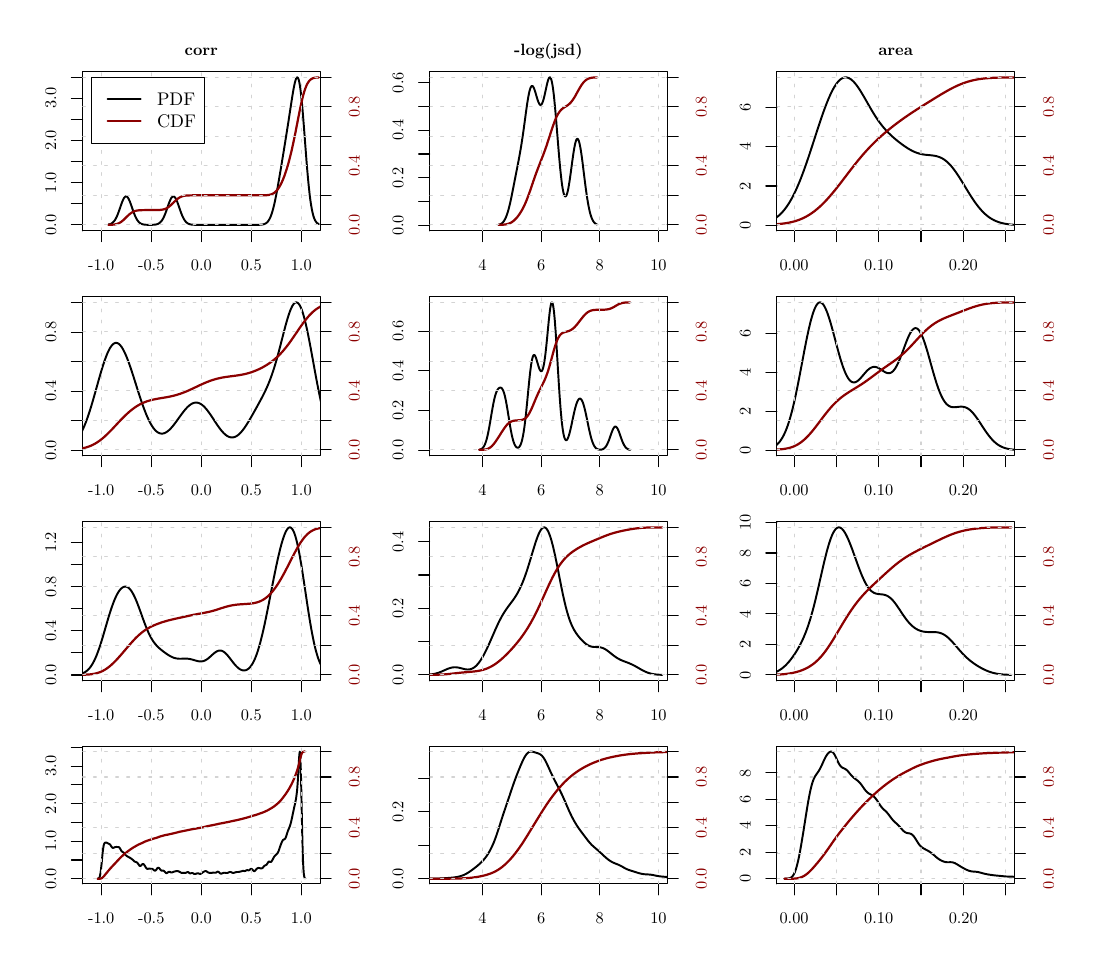
\begin{tikzpicture}[x=1pt,y=1pt]
\definecolor{fillColor}{RGB}{255,255,255}
\path[use as bounding box,fill=fillColor,fill opacity=0.00] (0,0) rectangle (376.36,325.21);
\begin{scope}
\path[clip] ( 19.80,251.83) rectangle (105.65,309.38);
\definecolor{drawColor}{RGB}{0,0,0}

\path[draw=drawColor,line width= 0.7pt,line join=round,line cap=round] ( 29.15,254.08) --
	( 29.30,254.11) --
	( 29.45,254.14) --
	( 29.60,254.17) --
	( 29.75,254.22) --
	( 29.90,254.27) --
	( 30.05,254.33) --
	( 30.19,254.41) --
	( 30.34,254.49) --
	( 30.49,254.58) --
	( 30.64,254.69) --
	( 30.79,254.82) --
	( 30.94,254.96) --
	( 31.09,255.12) --
	( 31.24,255.30) --
	( 31.38,255.49) --
	( 31.53,255.71) --
	( 31.68,255.95) --
	( 31.83,256.22) --
	( 31.98,256.50) --
	( 32.13,256.80) --
	( 32.28,257.13) --
	( 32.43,257.48) --
	( 32.58,257.85) --
	( 32.72,258.23) --
	( 32.87,258.63) --
	( 33.02,259.05) --
	( 33.17,259.47) --
	( 33.32,259.90) --
	( 33.47,260.34) --
	( 33.62,260.77) --
	( 33.77,261.20) --
	( 33.91,261.61) --
	( 34.06,262.01) --
	( 34.21,262.39) --
	( 34.36,262.75) --
	( 34.51,263.08) --
	( 34.66,263.37) --
	( 34.81,263.63) --
	( 34.96,263.84) --
	( 35.11,264.01) --
	( 35.25,264.14) --
	( 35.40,264.22) --
	( 35.55,264.25) --
	( 35.70,264.22) --
	( 35.85,264.15) --
	( 36.00,264.03) --
	( 36.15,263.87) --
	( 36.30,263.66) --
	( 36.44,263.41) --
	( 36.59,263.11) --
	( 36.74,262.79) --
	( 36.89,262.44) --
	( 37.04,262.06) --
	( 37.19,261.66) --
	( 37.34,261.25) --
	( 37.49,260.82) --
	( 37.64,260.39) --
	( 37.78,259.96) --
	( 37.93,259.53) --
	( 38.08,259.10) --
	( 38.23,258.69) --
	( 38.38,258.28) --
	( 38.53,257.90) --
	( 38.68,257.52) --
	( 38.83,257.17) --
	( 38.97,256.84) --
	( 39.12,256.54) --
	( 39.27,256.25) --
	( 39.42,255.98) --
	( 39.57,255.74) --
	( 39.72,255.52) --
	( 39.87,255.32) --
	( 40.02,255.14) --
	( 40.17,254.98) --
	( 40.31,254.83) --
	( 40.46,254.71) --
	( 40.61,254.60) --
	( 40.76,254.50) --
	( 40.91,254.42) --
	( 41.06,254.34) --
	( 41.21,254.28) --
	( 41.36,254.23) --
	( 41.50,254.18) --
	( 41.65,254.14) --
	( 41.80,254.11) --
	( 41.95,254.08) --
	( 42.10,254.06) --
	( 42.25,254.04) --
	( 42.40,254.03) --
	( 42.55,254.01) --
	( 42.69,254.00) --
	( 42.84,253.99) --
	( 42.99,253.99) --
	( 43.14,253.98) --
	( 43.29,253.98) --
	( 43.44,253.98) --
	( 43.59,253.97) --
	( 43.74,253.97) --
	( 43.89,253.97) --
	( 44.03,253.97) --
	( 44.18,253.97) --
	( 44.33,253.97) --
	( 44.48,253.97) --
	( 44.63,253.97) --
	( 44.78,253.98) --
	( 44.93,253.98) --
	( 45.08,253.98) --
	( 45.22,253.99) --
	( 45.37,254.00) --
	( 45.52,254.00) --
	( 45.67,254.01) --
	( 45.82,254.03) --
	( 45.97,254.04) --
	( 46.12,254.06) --
	( 46.27,254.09) --
	( 46.42,254.11) --
	( 46.56,254.15) --
	( 46.71,254.19) --
	( 46.86,254.23) --
	( 47.01,254.29) --
	( 47.16,254.35) --
	( 47.31,254.43) --
	( 47.46,254.51) --
	( 47.61,254.61) --
	( 47.75,254.72) --
	( 47.90,254.85) --
	( 48.05,255.00) --
	( 48.20,255.16) --
	( 48.35,255.34) --
	( 48.50,255.55) --
	( 48.65,255.77) --
	( 48.80,256.02) --
	( 48.95,256.28) --
	( 49.09,256.57) --
	( 49.24,256.88) --
	( 49.39,257.22) --
	( 49.54,257.57) --
	( 49.69,257.94) --
	( 49.84,258.33) --
	( 49.99,258.74) --
	( 50.14,259.15) --
	( 50.28,259.58) --
	( 50.43,260.01) --
	( 50.58,260.44) --
	( 50.73,260.87) --
	( 50.88,261.30) --
	( 51.03,261.71) --
	( 51.18,262.10) --
	( 51.33,262.48) --
	( 51.48,262.83) --
	( 51.62,263.15) --
	( 51.77,263.44) --
	( 51.92,263.68) --
	( 52.07,263.88) --
	( 52.22,264.04) --
	( 52.37,264.16) --
	( 52.52,264.23) --
	( 52.67,264.24) --
	( 52.81,264.20) --
	( 52.96,264.12) --
	( 53.11,263.99) --
	( 53.26,263.82) --
	( 53.41,263.60) --
	( 53.56,263.33) --
	( 53.71,263.03) --
	( 53.86,262.70) --
	( 54.01,262.35) --
	( 54.15,261.97) --
	( 54.30,261.56) --
	( 54.45,261.14) --
	( 54.60,260.72) --
	( 54.75,260.29) --
	( 54.90,259.85) --
	( 55.05,259.42) --
	( 55.20,259.00) --
	( 55.34,258.59) --
	( 55.49,258.19) --
	( 55.64,257.81) --
	( 55.79,257.44) --
	( 55.94,257.09) --
	( 56.09,256.77) --
	( 56.24,256.47) --
	( 56.39,256.18) --
	( 56.54,255.92) --
	( 56.68,255.69) --
	( 56.83,255.47) --
	( 56.98,255.28) --
	( 57.13,255.10) --
	( 57.28,254.94) --
	( 57.43,254.80) --
	( 57.58,254.68) --
	( 57.73,254.57) --
	( 57.87,254.48) --
	( 58.02,254.40) --
	( 58.17,254.33) --
	( 58.32,254.27) --
	( 58.47,254.21) --
	( 58.62,254.17) --
	( 58.77,254.13) --
	( 58.92,254.10) --
	( 59.07,254.08) --
	( 59.21,254.05) --
	( 59.36,254.04) --
	( 59.51,254.02) --
	( 59.66,254.01) --
	( 59.81,254.00) --
	( 59.96,253.99) --
	( 60.11,253.99) --
	( 60.26,253.98) --
	( 60.40,253.98) --
	( 60.55,253.97) --
	( 60.70,253.97) --
	( 60.85,253.97) --
	( 61.00,253.97) --
	( 61.15,253.97) --
	( 61.30,253.97) --
	( 61.45,253.96) --
	( 61.60,253.96) --
	( 61.74,253.96) --
	( 61.89,253.96) --
	( 62.04,253.96) --
	( 62.19,253.96) --
	( 62.34,253.96) --
	( 62.49,253.96) --
	( 62.64,253.96) --
	( 62.79,253.96) --
	( 62.93,253.96) --
	( 63.08,253.96) --
	( 63.23,253.96) --
	( 63.38,253.96) --
	( 63.53,253.96) --
	( 63.68,253.96) --
	( 63.83,253.96) --
	( 63.98,253.96) --
	( 64.12,253.96) --
	( 64.27,253.96) --
	( 64.42,253.96) --
	( 64.57,253.96) --
	( 64.72,253.96) --
	( 64.87,253.96) --
	( 65.02,253.96) --
	( 65.17,253.96) --
	( 65.32,253.96) --
	( 65.46,253.96) --
	( 65.61,253.96) --
	( 65.76,253.96) --
	( 65.91,253.96) --
	( 66.06,253.96) --
	( 66.21,253.96) --
	( 66.36,253.96) --
	( 66.51,253.96) --
	( 66.65,253.96) --
	( 66.80,253.96) --
	( 66.95,253.96) --
	( 67.10,253.96) --
	( 67.25,253.96) --
	( 67.40,253.96) --
	( 67.55,253.96) --
	( 67.70,253.96) --
	( 67.85,253.96) --
	( 67.99,253.96) --
	( 68.14,253.96) --
	( 68.29,253.96) --
	( 68.44,253.96) --
	( 68.59,253.96) --
	( 68.74,253.96) --
	( 68.89,253.96) --
	( 69.04,253.96) --
	( 69.18,253.96) --
	( 69.33,253.96) --
	( 69.48,253.96) --
	( 69.63,253.96) --
	( 69.78,253.96) --
	( 69.93,253.96) --
	( 70.08,253.96) --
	( 70.23,253.96) --
	( 70.38,253.96) --
	( 70.52,253.96) --
	( 70.67,253.96) --
	( 70.82,253.96) --
	( 70.97,253.96) --
	( 71.12,253.96) --
	( 71.27,253.96) --
	( 71.42,253.96) --
	( 71.57,253.96) --
	( 71.71,253.96) --
	( 71.86,253.96) --
	( 72.01,253.96) --
	( 72.16,253.96) --
	( 72.31,253.96) --
	( 72.46,253.96) --
	( 72.61,253.96) --
	( 72.76,253.96) --
	( 72.91,253.96) --
	( 73.05,253.96) --
	( 73.20,253.96) --
	( 73.35,253.96) --
	( 73.50,253.96) --
	( 73.65,253.96) --
	( 73.80,253.96) --
	( 73.95,253.96) --
	( 74.10,253.96) --
	( 74.24,253.96) --
	( 74.39,253.96) --
	( 74.54,253.96) --
	( 74.69,253.96) --
	( 74.84,253.96) --
	( 74.99,253.96) --
	( 75.14,253.96) --
	( 75.29,253.96) --
	( 75.44,253.96) --
	( 75.58,253.96) --
	( 75.73,253.96) --
	( 75.88,253.96) --
	( 76.03,253.96) --
	( 76.18,253.96) --
	( 76.33,253.96) --
	( 76.48,253.96) --
	( 76.63,253.96) --
	( 76.77,253.96) --
	( 76.92,253.96) --
	( 77.07,253.96) --
	( 77.22,253.96) --
	( 77.37,253.96) --
	( 77.52,253.96) --
	( 77.67,253.96) --
	( 77.82,253.96) --
	( 77.97,253.96) --
	( 78.11,253.96) --
	( 78.26,253.96) --
	( 78.41,253.96) --
	( 78.56,253.96) --
	( 78.71,253.96) --
	( 78.86,253.96) --
	( 79.01,253.96) --
	( 79.16,253.96) --
	( 79.30,253.96) --
	( 79.45,253.96) --
	( 79.60,253.96) --
	( 79.75,253.96) --
	( 79.90,253.96) --
	( 80.05,253.96) --
	( 80.20,253.96) --
	( 80.35,253.96) --
	( 80.50,253.96) --
	( 80.64,253.96) --
	( 80.79,253.96) --
	( 80.94,253.96) --
	( 81.09,253.96) --
	( 81.24,253.96) --
	( 81.39,253.96) --
	( 81.54,253.96) --
	( 81.69,253.96) --
	( 81.83,253.96) --
	( 81.98,253.96) --
	( 82.13,253.96) --
	( 82.28,253.96) --
	( 82.43,253.96) --
	( 82.58,253.97) --
	( 82.73,253.97) --
	( 82.88,253.97) --
	( 83.02,253.97) --
	( 83.17,253.97) --
	( 83.32,253.97) --
	( 83.47,253.98) --
	( 83.62,253.98) --
	( 83.77,253.98) --
	( 83.92,253.99) --
	( 84.07,254.00) --
	( 84.22,254.01) --
	( 84.36,254.02) --
	( 84.51,254.03) --
	( 84.66,254.05) --
	( 84.81,254.07) --
	( 84.96,254.10) --
	( 85.11,254.13) --
	( 85.26,254.16) --
	( 85.41,254.21) --
	( 85.55,254.26) --
	( 85.70,254.32) --
	( 85.85,254.39) --
	( 86.00,254.47) --
	( 86.15,254.57) --
	( 86.30,254.68) --
	( 86.45,254.80) --
	( 86.60,254.94) --
	( 86.75,255.11) --
	( 86.89,255.30) --
	( 87.04,255.50) --
	( 87.19,255.74) --
	( 87.34,255.99) --
	( 87.49,256.28) --
	( 87.64,256.59) --
	( 87.79,256.94) --
	( 87.94,257.32) --
	( 88.08,257.72) --
	( 88.23,258.16) --
	( 88.38,258.64) --
	( 88.53,259.15) --
	( 88.68,259.69) --
	( 88.83,260.26) --
	( 88.98,260.86) --
	( 89.13,261.50) --
	( 89.28,262.16) --
	( 89.42,262.86) --
	( 89.57,263.58) --
	( 89.72,264.32) --
	( 89.87,265.08) --
	( 90.02,265.87) --
	( 90.17,266.67) --
	( 90.32,267.49) --
	( 90.47,268.33) --
	( 90.61,269.18) --
	( 90.76,270.04) --
	( 90.91,270.91) --
	( 91.06,271.78) --
	( 91.21,272.67) --
	( 91.36,273.56) --
	( 91.51,274.45) --
	( 91.66,275.35) --
	( 91.81,276.25) --
	( 91.95,277.15) --
	( 92.10,278.06) --
	( 92.25,278.96) --
	( 92.40,279.87) --
	( 92.55,280.79) --
	( 92.70,281.70) --
	( 92.85,282.62) --
	( 93.00,283.54) --
	( 93.14,284.46) --
	( 93.29,285.39) --
	( 93.44,286.32) --
	( 93.59,287.26) --
	( 93.74,288.20) --
	( 93.89,289.15) --
	( 94.04,290.10) --
	( 94.19,291.05) --
	( 94.34,292.02) --
	( 94.48,292.98) --
	( 94.63,293.95) --
	( 94.78,294.93) --
	( 94.93,295.90) --
	( 95.08,296.87) --
	( 95.23,297.84) --
	( 95.38,298.80) --
	( 95.53,299.75) --
	( 95.67,300.67) --
	( 95.82,301.57) --
	( 95.97,302.43) --
	( 96.12,303.26) --
	( 96.27,304.04) --
	( 96.42,304.76) --
	( 96.57,305.40) --
	( 96.72,305.96) --
	( 96.87,306.43) --
	( 97.01,306.82) --
	( 97.16,307.10) --
	( 97.31,307.23) --
	( 97.46,307.24) --
	( 97.61,307.12) --
	( 97.76,306.87) --
	( 97.91,306.48) --
	( 98.06,305.93) --
	( 98.20,305.21) --
	( 98.35,304.35) --
	( 98.50,303.35) --
	( 98.65,302.22) --
	( 98.80,300.95) --
	( 98.95,299.53) --
	( 99.10,297.99) --
	( 99.25,296.36) --
	( 99.40,294.64) --
	( 99.54,292.84) --
	( 99.69,290.97) --
	( 99.84,289.05) --
	( 99.99,287.09) --
	(100.14,285.12) --
	(100.29,283.15) --
	(100.44,281.18) --
	(100.59,279.25) --
	(100.73,277.35) --
	(100.88,275.51) --
	(101.03,273.72) --
	(101.18,272.00) --
	(101.33,270.36) --
	(101.48,268.81) --
	(101.63,267.35) --
	(101.78,265.97) --
	(101.92,264.68) --
	(102.07,263.49) --
	(102.22,262.41) --
	(102.37,261.41) --
	(102.52,260.50) --
	(102.67,259.67) --
	(102.82,258.92) --
	(102.97,258.25) --
	(103.12,257.66) --
	(103.26,257.14) --
	(103.41,256.67) --
	(103.56,256.26) --
	(103.71,255.91) --
	(103.86,255.60) --
	(104.01,255.34) --
	(104.16,255.11) --
	(104.31,254.92) --
	(104.45,254.75) --
	(104.60,254.61) --
	(104.75,254.49) --
	(104.90,254.40) --
	(105.05,254.31) --
	(105.20,254.25);
\end{scope}
\begin{scope}
\path[clip] (  0.00,  0.00) rectangle (376.36,325.21);
\definecolor{drawColor}{RGB}{0,0,0}

\path[draw=drawColor,line width= 0.4pt,line join=round,line cap=round] ( 26.59,251.83) -- ( 98.86,251.83);

\path[draw=drawColor,line width= 0.4pt,line join=round,line cap=round] ( 26.59,251.83) -- ( 26.59,247.87);

\path[draw=drawColor,line width= 0.4pt,line join=round,line cap=round] ( 44.66,251.83) -- ( 44.66,247.87);

\path[draw=drawColor,line width= 0.4pt,line join=round,line cap=round] ( 62.73,251.83) -- ( 62.73,247.87);

\path[draw=drawColor,line width= 0.4pt,line join=round,line cap=round] ( 80.79,251.83) -- ( 80.79,247.87);

\path[draw=drawColor,line width= 0.4pt,line join=round,line cap=round] ( 98.86,251.83) -- ( 98.86,247.87);

\node[text=drawColor,anchor=base,inner sep=0pt, outer sep=0pt, scale=  0.59] at ( 26.59,237.58) {-1.0};

\node[text=drawColor,anchor=base,inner sep=0pt, outer sep=0pt, scale=  0.59] at ( 44.66,237.58) {-0.5};

\node[text=drawColor,anchor=base,inner sep=0pt, outer sep=0pt, scale=  0.59] at ( 62.73,237.58) {0.0};

\node[text=drawColor,anchor=base,inner sep=0pt, outer sep=0pt, scale=  0.59] at ( 80.79,237.58) {0.5};

\node[text=drawColor,anchor=base,inner sep=0pt, outer sep=0pt, scale=  0.59] at ( 98.86,237.58) {1.0};

\path[draw=drawColor,line width= 0.4pt,line join=round,line cap=round] ( 19.80,253.96) -- ( 19.80,307.34);

\path[draw=drawColor,line width= 0.4pt,line join=round,line cap=round] ( 19.80,253.96) -- ( 15.84,253.96);

\path[draw=drawColor,line width= 0.4pt,line join=round,line cap=round] ( 19.80,261.59) -- ( 15.84,261.59);

\path[draw=drawColor,line width= 0.4pt,line join=round,line cap=round] ( 19.80,269.21) -- ( 15.84,269.21);

\path[draw=drawColor,line width= 0.4pt,line join=round,line cap=round] ( 19.80,276.84) -- ( 15.84,276.84);

\path[draw=drawColor,line width= 0.4pt,line join=round,line cap=round] ( 19.80,284.46) -- ( 15.84,284.46);

\path[draw=drawColor,line width= 0.4pt,line join=round,line cap=round] ( 19.80,292.09) -- ( 15.84,292.09);

\path[draw=drawColor,line width= 0.4pt,line join=round,line cap=round] ( 19.80,299.71) -- ( 15.84,299.71);

\path[draw=drawColor,line width= 0.4pt,line join=round,line cap=round] ( 19.80,307.34) -- ( 15.84,307.34);

\node[text=drawColor,rotate= 90.00,anchor=base,inner sep=0pt, outer sep=0pt, scale=  0.59] at ( 10.30,253.96) {0.0};

\node[text=drawColor,rotate= 90.00,anchor=base,inner sep=0pt, outer sep=0pt, scale=  0.59] at ( 10.30,269.21) {1.0};

\node[text=drawColor,rotate= 90.00,anchor=base,inner sep=0pt, outer sep=0pt, scale=  0.59] at ( 10.30,284.46) {2.0};

\node[text=drawColor,rotate= 90.00,anchor=base,inner sep=0pt, outer sep=0pt, scale=  0.59] at ( 10.30,299.71) {3.0};

\path[draw=drawColor,line width= 0.4pt,line join=round,line cap=round] ( 19.80,251.83) --
	(105.65,251.83) --
	(105.65,309.38) --
	( 19.80,309.38) --
	( 19.80,251.83);
\end{scope}
\begin{scope}
\path[clip] ( 19.80,251.83) rectangle (105.65,309.38);
\definecolor{drawColor}{RGB}{139,0,0}

\path[draw=drawColor,line width= 0.8pt,line join=round,line cap=round] ( 29.15,253.97) --
	( 29.30,253.97) --
	( 29.45,253.97) --
	( 29.60,253.98) --
	( 29.75,253.98) --
	( 29.90,253.98) --
	( 30.05,253.99) --
	( 30.19,253.99) --
	( 30.34,254.00) --
	( 30.49,254.01) --
	( 30.64,254.02) --
	( 30.79,254.03) --
	( 30.94,254.04) --
	( 31.09,254.06) --
	( 31.24,254.08) --
	( 31.38,254.10) --
	( 31.53,254.12) --
	( 31.68,254.15) --
	( 31.83,254.18) --
	( 31.98,254.21) --
	( 32.13,254.25) --
	( 32.28,254.29) --
	( 32.43,254.34) --
	( 32.58,254.39) --
	( 32.72,254.45) --
	( 32.87,254.52) --
	( 33.02,254.59) --
	( 33.17,254.66) --
	( 33.32,254.75) --
	( 33.47,254.83) --
	( 33.62,254.93) --
	( 33.77,255.03) --
	( 33.91,255.14) --
	( 34.06,255.25) --
	( 34.21,255.37) --
	( 34.36,255.49) --
	( 34.51,255.62) --
	( 34.66,255.75) --
	( 34.81,255.89) --
	( 34.96,256.03) --
	( 35.11,256.18) --
	( 35.25,256.32) --
	( 35.40,256.47) --
	( 35.55,256.62) --
	( 35.70,256.77) --
	( 35.85,256.91) --
	( 36.00,257.06) --
	( 36.15,257.20) --
	( 36.30,257.34) --
	( 36.44,257.48) --
	( 36.59,257.62) --
	( 36.74,257.74) --
	( 36.89,257.87) --
	( 37.04,257.99) --
	( 37.19,258.10) --
	( 37.34,258.21) --
	( 37.49,258.31) --
	( 37.64,258.41) --
	( 37.78,258.50) --
	( 37.93,258.58) --
	( 38.08,258.66) --
	( 38.23,258.73) --
	( 38.38,258.79) --
	( 38.53,258.85) --
	( 38.68,258.91) --
	( 38.83,258.95) --
	( 38.97,259.00) --
	( 39.12,259.04) --
	( 39.27,259.07) --
	( 39.42,259.10) --
	( 39.57,259.13) --
	( 39.72,259.15) --
	( 39.87,259.17) --
	( 40.02,259.19) --
	( 40.17,259.21) --
	( 40.31,259.22) --
	( 40.46,259.23) --
	( 40.61,259.24) --
	( 40.76,259.25) --
	( 40.91,259.26) --
	( 41.06,259.26) --
	( 41.21,259.27) --
	( 41.36,259.27) --
	( 41.50,259.28) --
	( 41.65,259.28) --
	( 41.80,259.28) --
	( 41.95,259.28) --
	( 42.10,259.28) --
	( 42.25,259.29) --
	( 42.40,259.29) --
	( 42.55,259.29) --
	( 42.69,259.29) --
	( 42.84,259.29) --
	( 42.99,259.29) --
	( 43.14,259.29) --
	( 43.29,259.29) --
	( 43.44,259.29) --
	( 43.59,259.29) --
	( 43.74,259.29) --
	( 43.89,259.29) --
	( 44.03,259.29) --
	( 44.18,259.29) --
	( 44.33,259.29) --
	( 44.48,259.29) --
	( 44.63,259.29) --
	( 44.78,259.29) --
	( 44.93,259.29) --
	( 45.08,259.29) --
	( 45.22,259.29) --
	( 45.37,259.29) --
	( 45.52,259.29) --
	( 45.67,259.29) --
	( 45.82,259.29) --
	( 45.97,259.30) --
	( 46.12,259.30) --
	( 46.27,259.30) --
	( 46.42,259.30) --
	( 46.56,259.30) --
	( 46.71,259.31) --
	( 46.86,259.31) --
	( 47.01,259.31) --
	( 47.16,259.32) --
	( 47.31,259.32) --
	( 47.46,259.33) --
	( 47.61,259.34) --
	( 47.75,259.35) --
	( 47.90,259.36) --
	( 48.05,259.38) --
	( 48.20,259.39) --
	( 48.35,259.41) --
	( 48.50,259.43) --
	( 48.65,259.46) --
	( 48.80,259.48) --
	( 48.95,259.51) --
	( 49.09,259.55) --
	( 49.24,259.59) --
	( 49.39,259.63) --
	( 49.54,259.68) --
	( 49.69,259.74) --
	( 49.84,259.80) --
	( 49.99,259.86) --
	( 50.14,259.93) --
	( 50.28,260.01) --
	( 50.43,260.09) --
	( 50.58,260.18) --
	( 50.73,260.28) --
	( 50.88,260.38) --
	( 51.03,260.49) --
	( 51.18,260.61) --
	( 51.33,260.73) --
	( 51.48,260.85) --
	( 51.62,260.98) --
	( 51.77,261.12) --
	( 51.92,261.25) --
	( 52.07,261.40) --
	( 52.22,261.54) --
	( 52.37,261.69) --
	( 52.52,261.83) --
	( 52.67,261.98) --
	( 52.81,262.13) --
	( 52.96,262.28) --
	( 53.11,262.42) --
	( 53.26,262.57) --
	( 53.41,262.71) --
	( 53.56,262.84) --
	( 53.71,262.98) --
	( 53.86,263.10) --
	( 54.01,263.23) --
	( 54.15,263.34) --
	( 54.30,263.46) --
	( 54.45,263.56) --
	( 54.60,263.66) --
	( 54.75,263.76) --
	( 54.90,263.85) --
	( 55.05,263.93) --
	( 55.20,264.00) --
	( 55.34,264.07) --
	( 55.49,264.14) --
	( 55.64,264.19) --
	( 55.79,264.25) --
	( 55.94,264.29) --
	( 56.09,264.34) --
	( 56.24,264.37) --
	( 56.39,264.41) --
	( 56.54,264.44) --
	( 56.68,264.46) --
	( 56.83,264.49) --
	( 56.98,264.51) --
	( 57.13,264.52) --
	( 57.28,264.54) --
	( 57.43,264.55) --
	( 57.58,264.56) --
	( 57.73,264.57) --
	( 57.87,264.58) --
	( 58.02,264.59) --
	( 58.17,264.59) --
	( 58.32,264.60) --
	( 58.47,264.60) --
	( 58.62,264.61) --
	( 58.77,264.61) --
	( 58.92,264.61) --
	( 59.07,264.61) --
	( 59.21,264.61) --
	( 59.36,264.61) --
	( 59.51,264.62) --
	( 59.66,264.62) --
	( 59.81,264.62) --
	( 59.96,264.62) --
	( 60.11,264.62) --
	( 60.26,264.62) --
	( 60.40,264.62) --
	( 60.55,264.62) --
	( 60.70,264.62) --
	( 60.85,264.62) --
	( 61.00,264.62) --
	( 61.15,264.62) --
	( 61.30,264.62) --
	( 61.45,264.62) --
	( 61.60,264.62) --
	( 61.74,264.62) --
	( 61.89,264.62) --
	( 62.04,264.62) --
	( 62.19,264.62) --
	( 62.34,264.62) --
	( 62.49,264.62) --
	( 62.64,264.62) --
	( 62.79,264.62) --
	( 62.93,264.62) --
	( 63.08,264.62) --
	( 63.23,264.62) --
	( 63.38,264.62) --
	( 63.53,264.62) --
	( 63.68,264.62) --
	( 63.83,264.62) --
	( 63.98,264.62) --
	( 64.12,264.62) --
	( 64.27,264.62) --
	( 64.42,264.62) --
	( 64.57,264.62) --
	( 64.72,264.62) --
	( 64.87,264.62) --
	( 65.02,264.62) --
	( 65.17,264.62) --
	( 65.32,264.62) --
	( 65.46,264.62) --
	( 65.61,264.62) --
	( 65.76,264.62) --
	( 65.91,264.62) --
	( 66.06,264.62) --
	( 66.21,264.62) --
	( 66.36,264.62) --
	( 66.51,264.62) --
	( 66.65,264.62) --
	( 66.80,264.62) --
	( 66.95,264.62) --
	( 67.10,264.62) --
	( 67.25,264.62) --
	( 67.40,264.62) --
	( 67.55,264.62) --
	( 67.70,264.62) --
	( 67.85,264.62) --
	( 67.99,264.62) --
	( 68.14,264.62) --
	( 68.29,264.62) --
	( 68.44,264.62) --
	( 68.59,264.62) --
	( 68.74,264.62) --
	( 68.89,264.62) --
	( 69.04,264.62) --
	( 69.18,264.62) --
	( 69.33,264.62) --
	( 69.48,264.62) --
	( 69.63,264.62) --
	( 69.78,264.62) --
	( 69.93,264.62) --
	( 70.08,264.62) --
	( 70.23,264.62) --
	( 70.38,264.62) --
	( 70.52,264.62) --
	( 70.67,264.62) --
	( 70.82,264.62) --
	( 70.97,264.62) --
	( 71.12,264.62) --
	( 71.27,264.62) --
	( 71.42,264.62) --
	( 71.57,264.62) --
	( 71.71,264.62) --
	( 71.86,264.62) --
	( 72.01,264.62) --
	( 72.16,264.62) --
	( 72.31,264.62) --
	( 72.46,264.62) --
	( 72.61,264.62) --
	( 72.76,264.62) --
	( 72.91,264.62) --
	( 73.05,264.62) --
	( 73.20,264.62) --
	( 73.35,264.62) --
	( 73.50,264.62) --
	( 73.65,264.62) --
	( 73.80,264.62) --
	( 73.95,264.62) --
	( 74.10,264.62) --
	( 74.24,264.62) --
	( 74.39,264.62) --
	( 74.54,264.62) --
	( 74.69,264.62) --
	( 74.84,264.62) --
	( 74.99,264.62) --
	( 75.14,264.62) --
	( 75.29,264.62) --
	( 75.44,264.62) --
	( 75.58,264.62) --
	( 75.73,264.62) --
	( 75.88,264.62) --
	( 76.03,264.62) --
	( 76.18,264.62) --
	( 76.33,264.62) --
	( 76.48,264.62) --
	( 76.63,264.62) --
	( 76.77,264.62) --
	( 76.92,264.62) --
	( 77.07,264.62) --
	( 77.22,264.62) --
	( 77.37,264.62) --
	( 77.52,264.62) --
	( 77.67,264.62) --
	( 77.82,264.62) --
	( 77.97,264.62) --
	( 78.11,264.62) --
	( 78.26,264.62) --
	( 78.41,264.62) --
	( 78.56,264.62) --
	( 78.71,264.62) --
	( 78.86,264.62) --
	( 79.01,264.62) --
	( 79.16,264.62) --
	( 79.30,264.62) --
	( 79.45,264.62) --
	( 79.60,264.62) --
	( 79.75,264.62) --
	( 79.90,264.62) --
	( 80.05,264.62) --
	( 80.20,264.62) --
	( 80.35,264.62) --
	( 80.50,264.62) --
	( 80.64,264.62) --
	( 80.79,264.62) --
	( 80.94,264.62) --
	( 81.09,264.62) --
	( 81.24,264.62) --
	( 81.39,264.62) --
	( 81.54,264.62) --
	( 81.69,264.62) --
	( 81.83,264.62) --
	( 81.98,264.62) --
	( 82.13,264.62) --
	( 82.28,264.62) --
	( 82.43,264.62) --
	( 82.58,264.62) --
	( 82.73,264.62) --
	( 82.88,264.62) --
	( 83.02,264.62) --
	( 83.17,264.62) --
	( 83.32,264.62) --
	( 83.47,264.62) --
	( 83.62,264.62) --
	( 83.77,264.62) --
	( 83.92,264.62) --
	( 84.07,264.62) --
	( 84.22,264.62) --
	( 84.36,264.62) --
	( 84.51,264.62) --
	( 84.66,264.62) --
	( 84.81,264.63) --
	( 84.96,264.63) --
	( 85.11,264.63) --
	( 85.26,264.63) --
	( 85.41,264.63) --
	( 85.55,264.64) --
	( 85.70,264.64) --
	( 85.85,264.65) --
	( 86.00,264.66) --
	( 86.15,264.66) --
	( 86.30,264.67) --
	( 86.45,264.68) --
	( 86.60,264.70) --
	( 86.75,264.71) --
	( 86.89,264.73) --
	( 87.04,264.75) --
	( 87.19,264.77) --
	( 87.34,264.80) --
	( 87.49,264.83) --
	( 87.64,264.87) --
	( 87.79,264.91) --
	( 87.94,264.95) --
	( 88.08,265.00) --
	( 88.23,265.06) --
	( 88.38,265.12) --
	( 88.53,265.19) --
	( 88.68,265.27) --
	( 88.83,265.36) --
	( 88.98,265.45) --
	( 89.13,265.56) --
	( 89.28,265.67) --
	( 89.42,265.79) --
	( 89.57,265.93) --
	( 89.72,266.07) --
	( 89.87,266.22) --
	( 90.02,266.39) --
	( 90.17,266.56) --
	( 90.32,266.75) --
	( 90.47,266.95) --
	( 90.61,267.17) --
	( 90.76,267.39) --
	( 90.91,267.63) --
	( 91.06,267.88) --
	( 91.21,268.14) --
	( 91.36,268.42) --
	( 91.51,268.70) --
	( 91.66,269.00) --
	( 91.81,269.32) --
	( 91.95,269.65) --
	( 92.10,269.98) --
	( 92.25,270.34) --
	( 92.40,270.70) --
	( 92.55,271.08) --
	( 92.70,271.47) --
	( 92.85,271.88) --
	( 93.00,272.30) --
	( 93.14,272.73) --
	( 93.29,273.18) --
	( 93.44,273.63) --
	( 93.59,274.11) --
	( 93.74,274.59) --
	( 93.89,275.09) --
	( 94.04,275.60) --
	( 94.19,276.13) --
	( 94.34,276.67) --
	( 94.48,277.22) --
	( 94.63,277.79) --
	( 94.78,278.37) --
	( 94.93,278.97) --
	( 95.08,279.58) --
	( 95.23,280.20) --
	( 95.38,280.84) --
	( 95.53,281.49) --
	( 95.67,282.16) --
	( 95.82,282.84) --
	( 95.97,283.53) --
	( 96.12,284.23) --
	( 96.27,284.94) --
	( 96.42,285.67) --
	( 96.57,286.41) --
	( 96.72,287.15) --
	( 96.87,287.90) --
	( 97.01,288.66) --
	( 97.16,289.42) --
	( 97.31,290.19) --
	( 97.46,290.96) --
	( 97.61,291.72) --
	( 97.76,292.49) --
	( 97.91,293.24) --
	( 98.06,294.00) --
	( 98.20,294.74) --
	( 98.35,295.47) --
	( 98.50,296.19) --
	( 98.65,296.89) --
	( 98.80,297.58) --
	( 98.95,298.24) --
	( 99.10,298.89) --
	( 99.25,299.51) --
	( 99.40,300.11) --
	( 99.54,300.68) --
	( 99.69,301.23) --
	( 99.84,301.75) --
	( 99.99,302.24) --
	(100.14,302.70) --
	(100.29,303.13) --
	(100.44,303.54) --
	(100.59,303.91) --
	(100.73,304.26) --
	(100.88,304.59) --
	(101.03,304.88) --
	(101.18,305.15) --
	(101.33,305.40) --
	(101.48,305.62) --
	(101.63,305.83) --
	(101.78,306.01) --
	(101.92,306.17) --
	(102.07,306.32) --
	(102.22,306.44) --
	(102.37,306.56) --
	(102.52,306.66) --
	(102.67,306.74) --
	(102.82,306.82) --
	(102.97,306.89) --
	(103.12,306.94) --
	(103.26,306.99) --
	(103.41,307.03) --
	(103.56,307.07) --
	(103.71,307.10) --
	(103.86,307.13) --
	(104.01,307.15) --
	(104.16,307.16) --
	(104.31,307.18) --
	(104.45,307.19) --
	(104.60,307.20) --
	(104.75,307.21) --
	(104.90,307.22) --
	(105.05,307.22) --
	(105.20,307.23);
\end{scope}
\begin{scope}
\path[clip] (  0.00,  0.00) rectangle (376.36,325.21);
\definecolor{drawColor}{RGB}{0,0,0}

\path[draw=drawColor,line width= 0.4pt,line join=round,line cap=round] (105.65,253.96) -- (105.65,307.24);

\path[draw=drawColor,line width= 0.4pt,line join=round,line cap=round] (105.65,253.96) -- (109.61,253.96);

\path[draw=drawColor,line width= 0.4pt,line join=round,line cap=round] (105.65,264.62) -- (109.61,264.62);

\path[draw=drawColor,line width= 0.4pt,line join=round,line cap=round] (105.65,275.27) -- (109.61,275.27);

\path[draw=drawColor,line width= 0.4pt,line join=round,line cap=round] (105.65,285.93) -- (109.61,285.93);

\path[draw=drawColor,line width= 0.4pt,line join=round,line cap=round] (105.65,296.59) -- (109.61,296.59);

\path[draw=drawColor,line width= 0.4pt,line join=round,line cap=round] (105.65,307.24) -- (109.61,307.24);
\definecolor{drawColor}{RGB}{139,0,0}

\node[text=drawColor,rotate= 90.00,anchor=base,inner sep=0pt, outer sep=0pt, scale=  0.59] at (119.91,253.96) {0.0};

\node[text=drawColor,rotate= 90.00,anchor=base,inner sep=0pt, outer sep=0pt, scale=  0.59] at (119.91,275.27) {0.4};

\node[text=drawColor,rotate= 90.00,anchor=base,inner sep=0pt, outer sep=0pt, scale=  0.59] at (119.91,296.59) {0.8};
\end{scope}
\begin{scope}
\path[clip] (  0.00,243.91) rectangle (125.45,325.21);
\definecolor{drawColor}{RGB}{0,0,0}

\node[text=drawColor,anchor=base,inner sep=0pt, outer sep=0pt, scale=  0.59] at ( 62.73,315.25) {\bfseries corr};
\end{scope}
\begin{scope}
\path[clip] ( 19.80,251.83) rectangle (105.65,309.38);
\definecolor{drawColor}{RGB}{211,211,211}

\path[draw=drawColor,line width= 0.4pt,dash pattern=on 1pt off 3pt ,line join=round,line cap=round] ( 26.59,251.83) -- ( 26.59,309.38);

\path[draw=drawColor,line width= 0.4pt,dash pattern=on 1pt off 3pt ,line join=round,line cap=round] ( 44.66,251.83) -- ( 44.66,309.38);

\path[draw=drawColor,line width= 0.4pt,dash pattern=on 1pt off 3pt ,line join=round,line cap=round] ( 62.73,251.83) -- ( 62.73,309.38);

\path[draw=drawColor,line width= 0.4pt,dash pattern=on 1pt off 3pt ,line join=round,line cap=round] ( 80.79,251.83) -- ( 80.79,309.38);

\path[draw=drawColor,line width= 0.4pt,dash pattern=on 1pt off 3pt ,line join=round,line cap=round] ( 98.86,251.83) -- ( 98.86,309.38);

\path[draw=drawColor,line width= 0.4pt,dash pattern=on 1pt off 3pt ,line join=round,line cap=round] ( 19.80,253.96) -- (105.65,253.96);

\path[draw=drawColor,line width= 0.4pt,dash pattern=on 1pt off 3pt ,line join=round,line cap=round] ( 19.80,264.62) -- (105.65,264.62);

\path[draw=drawColor,line width= 0.4pt,dash pattern=on 1pt off 3pt ,line join=round,line cap=round] ( 19.80,275.27) -- (105.65,275.27);

\path[draw=drawColor,line width= 0.4pt,dash pattern=on 1pt off 3pt ,line join=round,line cap=round] ( 19.80,285.93) -- (105.65,285.93);

\path[draw=drawColor,line width= 0.4pt,dash pattern=on 1pt off 3pt ,line join=round,line cap=round] ( 19.80,296.59) -- (105.65,296.59);

\path[draw=drawColor,line width= 0.4pt,dash pattern=on 1pt off 3pt ,line join=round,line cap=round] ( 19.80,307.24) -- (105.65,307.24);
\definecolor{drawColor}{RGB}{0,0,0}
\definecolor{fillColor}{RGB}{255,255,255}

\path[draw=drawColor,line width= 0.4pt,line join=round,line cap=round,fill=fillColor] ( 22.98,307.24) rectangle ( 63.82,283.48);

\path[draw=drawColor,line width= 0.7pt,line join=round,line cap=round] ( 28.92,299.32) -- ( 40.80,299.32);
\definecolor{drawColor}{RGB}{139,0,0}

\path[draw=drawColor,line width= 0.8pt,line join=round,line cap=round] ( 28.92,291.40) -- ( 40.80,291.40);
\definecolor{drawColor}{RGB}{0,0,0}

\node[text=drawColor,anchor=base west,inner sep=0pt, outer sep=0pt, scale=  0.66] at ( 46.74,297.05) {PDF};

\node[text=drawColor,anchor=base west,inner sep=0pt, outer sep=0pt, scale=  0.66] at ( 46.74,289.13) {CDF};
\end{scope}
\begin{scope}
\path[clip] (145.25,251.83) rectangle (231.11,309.38);
\definecolor{drawColor}{RGB}{0,0,0}

\path[draw=drawColor,line width= 0.7pt,line join=round,line cap=round] (170.12,253.96) --
	(170.19,253.98) --
	(170.26,254.00) --
	(170.33,254.02) --
	(170.40,254.04) --
	(170.47,254.06) --
	(170.54,254.08) --
	(170.61,254.11) --
	(170.68,254.14) --
	(170.75,254.17) --
	(170.82,254.20) --
	(170.89,254.24) --
	(170.96,254.27) --
	(171.03,254.31) --
	(171.10,254.35) --
	(171.17,254.40) --
	(171.24,254.45) --
	(171.31,254.50) --
	(171.38,254.56) --
	(171.45,254.61) --
	(171.52,254.68) --
	(171.59,254.74) --
	(171.66,254.81) --
	(171.73,254.89) --
	(171.80,254.97) --
	(171.87,255.05) --
	(171.94,255.14) --
	(172.01,255.23) --
	(172.08,255.33) --
	(172.15,255.43) --
	(172.22,255.54) --
	(172.28,255.65) --
	(172.35,255.77) --
	(172.42,255.90) --
	(172.49,256.03) --
	(172.56,256.17) --
	(172.63,256.31) --
	(172.70,256.46) --
	(172.77,256.61) --
	(172.84,256.78) --
	(172.91,256.95) --
	(172.98,257.12) --
	(173.05,257.30) --
	(173.12,257.49) --
	(173.19,257.69) --
	(173.26,257.89) --
	(173.33,258.10) --
	(173.40,258.32) --
	(173.47,258.54) --
	(173.54,258.78) --
	(173.61,259.01) --
	(173.68,259.26) --
	(173.75,259.51) --
	(173.82,259.77) --
	(173.89,260.03) --
	(173.96,260.30) --
	(174.03,260.58) --
	(174.10,260.86) --
	(174.17,261.15) --
	(174.24,261.45) --
	(174.31,261.75) --
	(174.38,262.06) --
	(174.45,262.37) --
	(174.52,262.68) --
	(174.59,263.00) --
	(174.66,263.33) --
	(174.73,263.66) --
	(174.80,263.99) --
	(174.86,264.33) --
	(174.93,264.67) --
	(175.00,265.01) --
	(175.07,265.36) --
	(175.14,265.71) --
	(175.21,266.06) --
	(175.28,266.41) --
	(175.35,266.76) --
	(175.42,267.12) --
	(175.49,267.48) --
	(175.56,267.83) --
	(175.63,268.19) --
	(175.70,268.55) --
	(175.77,268.91) --
	(175.84,269.27) --
	(175.91,269.63) --
	(175.98,269.99) --
	(176.05,270.35) --
	(176.12,270.70) --
	(176.19,271.06) --
	(176.26,271.42) --
	(176.33,271.78) --
	(176.40,272.13) --
	(176.47,272.49) --
	(176.54,272.84) --
	(176.61,273.20) --
	(176.68,273.55) --
	(176.75,273.91) --
	(176.82,274.26) --
	(176.89,274.62) --
	(176.96,274.97) --
	(177.03,275.33) --
	(177.10,275.69) --
	(177.17,276.05) --
	(177.24,276.41) --
	(177.31,276.77) --
	(177.38,277.13) --
	(177.44,277.50) --
	(177.51,277.87) --
	(177.58,278.24) --
	(177.65,278.62) --
	(177.72,279.00) --
	(177.79,279.38) --
	(177.86,279.77) --
	(177.93,280.16) --
	(178.00,280.56) --
	(178.07,280.97) --
	(178.14,281.37) --
	(178.21,281.79) --
	(178.28,282.21) --
	(178.35,282.64) --
	(178.42,283.07) --
	(178.49,283.51) --
	(178.56,283.95) --
	(178.63,284.41) --
	(178.70,284.87) --
	(178.77,285.33) --
	(178.84,285.80) --
	(178.91,286.28) --
	(178.98,286.76) --
	(179.05,287.25) --
	(179.12,287.74) --
	(179.19,288.24) --
	(179.26,288.74) --
	(179.33,289.25) --
	(179.40,289.76) --
	(179.47,290.27) --
	(179.54,290.79) --
	(179.61,291.31) --
	(179.68,291.82) --
	(179.75,292.34) --
	(179.82,292.86) --
	(179.89,293.38) --
	(179.96,293.89) --
	(180.02,294.40) --
	(180.09,294.91) --
	(180.16,295.41) --
	(180.23,295.91) --
	(180.30,296.39) --
	(180.37,296.88) --
	(180.44,297.35) --
	(180.51,297.81) --
	(180.58,298.27) --
	(180.65,298.71) --
	(180.72,299.14) --
	(180.79,299.56) --
	(180.86,299.96) --
	(180.93,300.34) --
	(181.00,300.72) --
	(181.07,301.07) --
	(181.14,301.41) --
	(181.21,301.74) --
	(181.28,302.04) --
	(181.35,302.32) --
	(181.42,302.59) --
	(181.49,302.83) --
	(181.56,303.05) --
	(181.63,303.26) --
	(181.70,303.44) --
	(181.77,303.60) --
	(181.84,303.74) --
	(181.91,303.86) --
	(181.98,303.96) --
	(182.05,304.04) --
	(182.12,304.09) --
	(182.19,304.13) --
	(182.26,304.14) --
	(182.33,304.14) --
	(182.40,304.11) --
	(182.47,304.07) --
	(182.54,304.01) --
	(182.60,303.93) --
	(182.67,303.83) --
	(182.74,303.72) --
	(182.81,303.59) --
	(182.88,303.45) --
	(182.95,303.29) --
	(183.02,303.12) --
	(183.09,302.94) --
	(183.16,302.75) --
	(183.23,302.55) --
	(183.30,302.33) --
	(183.37,302.11) --
	(183.44,301.89) --
	(183.51,301.66) --
	(183.58,301.42) --
	(183.65,301.19) --
	(183.72,300.94) --
	(183.79,300.70) --
	(183.86,300.46) --
	(183.93,300.22) --
	(184.00,299.99) --
	(184.07,299.75) --
	(184.14,299.53) --
	(184.21,299.31) --
	(184.28,299.09) --
	(184.35,298.88) --
	(184.42,298.69) --
	(184.49,298.50) --
	(184.56,298.32) --
	(184.63,298.15) --
	(184.70,298.00) --
	(184.77,297.86) --
	(184.84,297.73) --
	(184.91,297.62) --
	(184.98,297.53) --
	(185.05,297.45) --
	(185.12,297.38) --
	(185.18,297.33) --
	(185.25,297.30) --
	(185.32,297.29) --
	(185.39,297.29) --
	(185.46,297.31) --
	(185.53,297.35) --
	(185.60,297.41) --
	(185.67,297.49) --
	(185.74,297.58) --
	(185.81,297.69) --
	(185.88,297.82) --
	(185.95,297.97) --
	(186.02,298.13) --
	(186.09,298.30) --
	(186.16,298.50) --
	(186.23,298.71) --
	(186.30,298.93) --
	(186.37,299.17) --
	(186.44,299.42) --
	(186.51,299.68) --
	(186.58,299.95) --
	(186.65,300.24) --
	(186.72,300.53) --
	(186.79,300.83) --
	(186.86,301.14) --
	(186.93,301.45) --
	(187.00,301.77) --
	(187.07,302.09) --
	(187.14,302.41) --
	(187.21,302.74) --
	(187.28,303.06) --
	(187.35,303.38) --
	(187.42,303.70) --
	(187.49,304.02) --
	(187.56,304.32) --
	(187.63,304.62) --
	(187.70,304.91) --
	(187.76,305.19) --
	(187.83,305.46) --
	(187.90,305.72) --
	(187.97,305.96) --
	(188.04,306.18) --
	(188.11,306.39) --
	(188.18,306.57) --
	(188.25,306.74) --
	(188.32,306.88) --
	(188.39,307.01) --
	(188.46,307.10) --
	(188.53,307.18) --
	(188.60,307.22) --
	(188.67,307.24) --
	(188.74,307.24) --
	(188.81,307.20) --
	(188.88,307.14) --
	(188.95,307.05) --
	(189.02,306.92) --
	(189.09,306.76) --
	(189.16,306.58) --
	(189.23,306.36) --
	(189.30,306.11) --
	(189.37,305.83) --
	(189.44,305.51) --
	(189.51,305.16) --
	(189.58,304.79) --
	(189.65,304.38) --
	(189.72,303.94) --
	(189.79,303.47) --
	(189.86,302.97) --
	(189.93,302.44) --
	(190.00,301.89) --
	(190.07,301.30) --
	(190.14,300.69) --
	(190.21,300.05) --
	(190.28,299.38) --
	(190.34,298.70) --
	(190.41,297.99) --
	(190.48,297.26) --
	(190.55,296.51) --
	(190.62,295.75) --
	(190.69,294.96) --
	(190.76,294.16) --
	(190.83,293.35) --
	(190.90,292.52) --
	(190.97,291.68) --
	(191.04,290.83) --
	(191.11,289.98) --
	(191.18,289.12) --
	(191.25,288.25) --
	(191.32,287.38) --
	(191.39,286.51) --
	(191.46,285.64) --
	(191.53,284.77) --
	(191.60,283.90) --
	(191.67,283.04) --
	(191.74,282.18) --
	(191.81,281.33) --
	(191.88,280.49) --
	(191.95,279.67) --
	(192.02,278.84) --
	(192.09,278.04) --
	(192.16,277.25) --
	(192.23,276.47) --
	(192.30,275.72) --
	(192.37,274.98) --
	(192.44,274.25) --
	(192.51,273.56) --
	(192.58,272.87) --
	(192.65,272.21) --
	(192.72,271.58) --
	(192.79,270.96) --
	(192.86,270.37) --
	(192.92,269.81) --
	(192.99,269.26) --
	(193.06,268.75) --
	(193.13,268.26) --
	(193.20,267.80) --
	(193.27,267.36) --
	(193.34,266.96) --
	(193.41,266.58) --
	(193.48,266.23) --
	(193.55,265.91) --
	(193.62,265.61) --
	(193.69,265.35) --
	(193.76,265.11) --
	(193.83,264.90) --
	(193.90,264.72) --
	(193.97,264.57) --
	(194.04,264.44) --
	(194.11,264.36) --
	(194.18,264.29) --
	(194.25,264.25) --
	(194.32,264.25) --
	(194.39,264.26) --
	(194.46,264.30) --
	(194.53,264.38) --
	(194.60,264.48) --
	(194.67,264.60) --
	(194.74,264.75) --
	(194.81,264.93) --
	(194.88,265.12) --
	(194.95,265.35) --
	(195.02,265.59) --
	(195.09,265.86) --
	(195.16,266.16) --
	(195.23,266.46) --
	(195.30,266.80) --
	(195.37,267.15) --
	(195.44,267.52) --
	(195.50,267.90) --
	(195.57,268.31) --
	(195.64,268.73) --
	(195.71,269.16) --
	(195.78,269.61) --
	(195.85,270.07) --
	(195.92,270.54) --
	(195.99,271.03) --
	(196.06,271.52) --
	(196.13,272.02) --
	(196.20,272.53) --
	(196.27,273.04) --
	(196.34,273.56) --
	(196.41,274.08) --
	(196.48,274.60) --
	(196.55,275.12) --
	(196.62,275.65) --
	(196.69,276.17) --
	(196.76,276.68) --
	(196.83,277.20) --
	(196.90,277.71) --
	(196.97,278.20) --
	(197.04,278.69) --
	(197.11,279.18) --
	(197.18,279.64) --
	(197.25,280.10) --
	(197.32,280.55) --
	(197.39,280.97) --
	(197.46,281.38) --
	(197.53,281.78) --
	(197.60,282.15) --
	(197.67,282.51) --
	(197.74,282.85) --
	(197.81,283.16) --
	(197.88,283.46) --
	(197.95,283.73) --
	(198.02,283.97) --
	(198.08,284.20) --
	(198.15,284.40) --
	(198.22,284.56) --
	(198.29,284.71) --
	(198.36,284.83) --
	(198.43,284.92) --
	(198.50,284.99) --
	(198.57,285.02) --
	(198.64,285.03) --
	(198.71,285.01) --
	(198.78,284.96) --
	(198.85,284.89) --
	(198.92,284.79) --
	(198.99,284.66) --
	(199.06,284.50) --
	(199.13,284.33) --
	(199.20,284.11) --
	(199.27,283.88) --
	(199.34,283.62) --
	(199.41,283.33) --
	(199.48,283.03) --
	(199.55,282.70) --
	(199.62,282.35) --
	(199.69,281.98) --
	(199.76,281.59) --
	(199.83,281.17) --
	(199.90,280.75) --
	(199.97,280.30) --
	(200.04,279.84) --
	(200.11,279.36) --
	(200.18,278.87) --
	(200.25,278.37) --
	(200.32,277.85) --
	(200.39,277.33) --
	(200.46,276.79) --
	(200.53,276.25) --
	(200.60,275.70) --
	(200.66,275.15) --
	(200.73,274.59) --
	(200.80,274.03) --
	(200.87,273.46) --
	(200.94,272.90) --
	(201.01,272.33) --
	(201.08,271.76) --
	(201.15,271.20) --
	(201.22,270.64) --
	(201.29,270.08) --
	(201.36,269.52) --
	(201.43,268.98) --
	(201.50,268.43) --
	(201.57,267.90) --
	(201.64,267.37) --
	(201.71,266.85) --
	(201.78,266.33) --
	(201.85,265.83) --
	(201.92,265.34) --
	(201.99,264.86) --
	(202.06,264.39) --
	(202.13,263.93) --
	(202.20,263.48) --
	(202.27,263.04) --
	(202.34,262.61) --
	(202.41,262.20) --
	(202.48,261.80) --
	(202.55,261.41) --
	(202.62,261.03) --
	(202.69,260.67) --
	(202.76,260.31) --
	(202.83,259.98) --
	(202.90,259.65) --
	(202.97,259.33) --
	(203.04,259.03) --
	(203.11,258.74) --
	(203.18,258.46) --
	(203.24,258.20) --
	(203.31,257.94) --
	(203.38,257.69) --
	(203.45,257.46) --
	(203.52,257.24) --
	(203.59,257.03) --
	(203.66,256.83) --
	(203.73,256.64) --
	(203.80,256.45) --
	(203.87,256.28) --
	(203.94,256.12) --
	(204.01,255.96) --
	(204.08,255.82) --
	(204.15,255.68) --
	(204.22,255.55) --
	(204.29,255.43) --
	(204.36,255.31) --
	(204.43,255.20) --
	(204.50,255.10) --
	(204.57,255.00) --
	(204.64,254.91) --
	(204.71,254.83) --
	(204.78,254.75) --
	(204.85,254.68) --
	(204.92,254.61) --
	(204.99,254.54) --
	(205.06,254.48) --
	(205.13,254.43) --
	(205.20,254.38) --
	(205.27,254.33) --
	(205.34,254.29) --
	(205.41,254.24) --
	(205.48,254.21) --
	(205.55,254.17) --
	(205.62,254.14) --
	(205.69,254.11) --
	(205.76,254.08);
\end{scope}
\begin{scope}
\path[clip] (  0.00,  0.00) rectangle (376.36,325.21);
\definecolor{drawColor}{RGB}{0,0,0}

\path[draw=drawColor,line width= 0.4pt,line join=round,line cap=round] (164.33,251.83) -- (227.93,251.83);

\path[draw=drawColor,line width= 0.4pt,line join=round,line cap=round] (164.33,251.83) -- (164.33,247.87);

\path[draw=drawColor,line width= 0.4pt,line join=round,line cap=round] (185.53,251.83) -- (185.53,247.87);

\path[draw=drawColor,line width= 0.4pt,line join=round,line cap=round] (206.73,251.83) -- (206.73,247.87);

\path[draw=drawColor,line width= 0.4pt,line join=round,line cap=round] (227.93,251.83) -- (227.93,247.87);

\node[text=drawColor,anchor=base,inner sep=0pt, outer sep=0pt, scale=  0.59] at (164.33,237.58) {4};

\node[text=drawColor,anchor=base,inner sep=0pt, outer sep=0pt, scale=  0.59] at (185.53,237.58) {6};

\node[text=drawColor,anchor=base,inner sep=0pt, outer sep=0pt, scale=  0.59] at (206.73,237.58) {8};

\node[text=drawColor,anchor=base,inner sep=0pt, outer sep=0pt, scale=  0.59] at (227.93,237.58) {10};

\path[draw=drawColor,line width= 0.4pt,line join=round,line cap=round] (145.25,253.79) -- (145.25,305.36);

\path[draw=drawColor,line width= 0.4pt,line join=round,line cap=round] (145.25,253.79) -- (141.29,253.79);

\path[draw=drawColor,line width= 0.4pt,line join=round,line cap=round] (145.25,262.38) -- (141.29,262.38);

\path[draw=drawColor,line width= 0.4pt,line join=round,line cap=round] (145.25,270.98) -- (141.29,270.98);

\path[draw=drawColor,line width= 0.4pt,line join=round,line cap=round] (145.25,279.57) -- (141.29,279.57);

\path[draw=drawColor,line width= 0.4pt,line join=round,line cap=round] (145.25,288.17) -- (141.29,288.17);

\path[draw=drawColor,line width= 0.4pt,line join=round,line cap=round] (145.25,296.76) -- (141.29,296.76);

\path[draw=drawColor,line width= 0.4pt,line join=round,line cap=round] (145.25,305.36) -- (141.29,305.36);

\node[text=drawColor,rotate= 90.00,anchor=base,inner sep=0pt, outer sep=0pt, scale=  0.59] at (135.75,253.79) {0.0};

\node[text=drawColor,rotate= 90.00,anchor=base,inner sep=0pt, outer sep=0pt, scale=  0.59] at (135.75,270.98) {0.2};

\node[text=drawColor,rotate= 90.00,anchor=base,inner sep=0pt, outer sep=0pt, scale=  0.59] at (135.75,288.17) {0.4};

\node[text=drawColor,rotate= 90.00,anchor=base,inner sep=0pt, outer sep=0pt, scale=  0.59] at (135.75,305.36) {0.6};

\path[draw=drawColor,line width= 0.4pt,line join=round,line cap=round] (145.25,251.83) --
	(231.11,251.83) --
	(231.11,309.38) --
	(145.25,309.38) --
	(145.25,251.83);
\end{scope}
\begin{scope}
\path[clip] (145.25,251.83) rectangle (231.11,309.38);
\definecolor{drawColor}{RGB}{139,0,0}

\path[draw=drawColor,line width= 0.8pt,line join=round,line cap=round] (170.12,253.97) --
	(170.19,253.97) --
	(170.26,253.97) --
	(170.33,253.97) --
	(170.40,253.97) --
	(170.47,253.97) --
	(170.54,253.98) --
	(170.61,253.98) --
	(170.68,253.98) --
	(170.75,253.98) --
	(170.82,253.98) --
	(170.89,253.98) --
	(170.96,253.98) --
	(171.03,253.99) --
	(171.10,253.99) --
	(171.17,253.99) --
	(171.24,253.99) --
	(171.31,254.00) --
	(171.38,254.00) --
	(171.45,254.00) --
	(171.52,254.01) --
	(171.59,254.01) --
	(171.66,254.01) --
	(171.73,254.02) --
	(171.80,254.02) --
	(171.87,254.03) --
	(171.94,254.03) --
	(172.01,254.04) --
	(172.08,254.05) --
	(172.15,254.05) --
	(172.22,254.06) --
	(172.28,254.07) --
	(172.35,254.07) --
	(172.42,254.08) --
	(172.49,254.09) --
	(172.56,254.10) --
	(172.63,254.11) --
	(172.70,254.12) --
	(172.77,254.13) --
	(172.84,254.14) --
	(172.91,254.16) --
	(172.98,254.17) --
	(173.05,254.18) --
	(173.12,254.20) --
	(173.19,254.21) --
	(173.26,254.23) --
	(173.33,254.25) --
	(173.40,254.26) --
	(173.47,254.28) --
	(173.54,254.30) --
	(173.61,254.32) --
	(173.68,254.35) --
	(173.75,254.37) --
	(173.82,254.39) --
	(173.89,254.42) --
	(173.96,254.44) --
	(174.03,254.47) --
	(174.10,254.50) --
	(174.17,254.53) --
	(174.24,254.56) --
	(174.31,254.59) --
	(174.38,254.62) --
	(174.45,254.66) --
	(174.52,254.69) --
	(174.59,254.73) --
	(174.66,254.77) --
	(174.73,254.81) --
	(174.80,254.85) --
	(174.86,254.89) --
	(174.93,254.93) --
	(175.00,254.98) --
	(175.07,255.03) --
	(175.14,255.07) --
	(175.21,255.12) --
	(175.28,255.17) --
	(175.35,255.23) --
	(175.42,255.28) --
	(175.49,255.33) --
	(175.56,255.39) --
	(175.63,255.45) --
	(175.70,255.51) --
	(175.77,255.57) --
	(175.84,255.63) --
	(175.91,255.70) --
	(175.98,255.76) --
	(176.05,255.83) --
	(176.12,255.90) --
	(176.19,255.97) --
	(176.26,256.04) --
	(176.33,256.11) --
	(176.40,256.18) --
	(176.47,256.26) --
	(176.54,256.34) --
	(176.61,256.41) --
	(176.68,256.49) --
	(176.75,256.58) --
	(176.82,256.66) --
	(176.89,256.74) --
	(176.96,256.83) --
	(177.03,256.91) --
	(177.10,257.00) --
	(177.17,257.09) --
	(177.24,257.18) --
	(177.31,257.28) --
	(177.38,257.37) --
	(177.44,257.47) --
	(177.51,257.56) --
	(177.58,257.66) --
	(177.65,257.76) --
	(177.72,257.87) --
	(177.79,257.97) --
	(177.86,258.07) --
	(177.93,258.18) --
	(178.00,258.29) --
	(178.07,258.40) --
	(178.14,258.51) --
	(178.21,258.62) --
	(178.28,258.74) --
	(178.35,258.86) --
	(178.42,258.97) --
	(178.49,259.09) --
	(178.56,259.22) --
	(178.63,259.34) --
	(178.70,259.47) --
	(178.77,259.59) --
	(178.84,259.72) --
	(178.91,259.85) --
	(178.98,259.99) --
	(179.05,260.12) --
	(179.12,260.26) --
	(179.19,260.40) --
	(179.26,260.54) --
	(179.33,260.68) --
	(179.40,260.83) --
	(179.47,260.98) --
	(179.54,261.13) --
	(179.61,261.28) --
	(179.68,261.43) --
	(179.75,261.59) --
	(179.82,261.75) --
	(179.89,261.91) --
	(179.96,262.07) --
	(180.02,262.23) --
	(180.09,262.40) --
	(180.16,262.57) --
	(180.23,262.74) --
	(180.30,262.91) --
	(180.37,263.09) --
	(180.44,263.26) --
	(180.51,263.44) --
	(180.58,263.62) --
	(180.65,263.80) --
	(180.72,263.99) --
	(180.79,264.17) --
	(180.86,264.36) --
	(180.93,264.55) --
	(181.00,264.74) --
	(181.07,264.93) --
	(181.14,265.13) --
	(181.21,265.32) --
	(181.28,265.52) --
	(181.35,265.71) --
	(181.42,265.91) --
	(181.49,266.11) --
	(181.56,266.31) --
	(181.63,266.51) --
	(181.70,266.72) --
	(181.77,266.92) --
	(181.84,267.12) --
	(181.91,267.33) --
	(181.98,267.53) --
	(182.05,267.74) --
	(182.12,267.94) --
	(182.19,268.15) --
	(182.26,268.35) --
	(182.33,268.56) --
	(182.40,268.76) --
	(182.47,268.97) --
	(182.54,269.17) --
	(182.60,269.38) --
	(182.67,269.58) --
	(182.74,269.78) --
	(182.81,269.99) --
	(182.88,270.19) --
	(182.95,270.39) --
	(183.02,270.59) --
	(183.09,270.79) --
	(183.16,270.99) --
	(183.23,271.19) --
	(183.30,271.39) --
	(183.37,271.59) --
	(183.44,271.79) --
	(183.51,271.98) --
	(183.58,272.18) --
	(183.65,272.37) --
	(183.72,272.56) --
	(183.79,272.75) --
	(183.86,272.94) --
	(183.93,273.13) --
	(184.00,273.32) --
	(184.07,273.51) --
	(184.14,273.70) --
	(184.21,273.88) --
	(184.28,274.07) --
	(184.35,274.25) --
	(184.42,274.44) --
	(184.49,274.62) --
	(184.56,274.80) --
	(184.63,274.98) --
	(184.70,275.16) --
	(184.77,275.34) --
	(184.84,275.52) --
	(184.91,275.70) --
	(184.98,275.88) --
	(185.05,276.05) --
	(185.12,276.23) --
	(185.18,276.41) --
	(185.25,276.59) --
	(185.32,276.76) --
	(185.39,276.94) --
	(185.46,277.12) --
	(185.53,277.30) --
	(185.60,277.47) --
	(185.67,277.65) --
	(185.74,277.83) --
	(185.81,278.01) --
	(185.88,278.19) --
	(185.95,278.37) --
	(186.02,278.55) --
	(186.09,278.73) --
	(186.16,278.91) --
	(186.23,279.09) --
	(186.30,279.28) --
	(186.37,279.46) --
	(186.44,279.65) --
	(186.51,279.83) --
	(186.58,280.02) --
	(186.65,280.21) --
	(186.72,280.40) --
	(186.79,280.59) --
	(186.86,280.78) --
	(186.93,280.97) --
	(187.00,281.17) --
	(187.07,281.37) --
	(187.14,281.56) --
	(187.21,281.76) --
	(187.28,281.96) --
	(187.35,282.16) --
	(187.42,282.37) --
	(187.49,282.57) --
	(187.56,282.77) --
	(187.63,282.98) --
	(187.70,283.19) --
	(187.76,283.40) --
	(187.83,283.61) --
	(187.90,283.82) --
	(187.97,284.03) --
	(188.04,284.24) --
	(188.11,284.46) --
	(188.18,284.67) --
	(188.25,284.89) --
	(188.32,285.11) --
	(188.39,285.32) --
	(188.46,285.54) --
	(188.53,285.76) --
	(188.60,285.97) --
	(188.67,286.19) --
	(188.74,286.41) --
	(188.81,286.63) --
	(188.88,286.85) --
	(188.95,287.06) --
	(189.02,287.28) --
	(189.09,287.50) --
	(189.16,287.71) --
	(189.23,287.93) --
	(189.30,288.14) --
	(189.37,288.35) --
	(189.44,288.57) --
	(189.51,288.78) --
	(189.58,288.98) --
	(189.65,289.19) --
	(189.72,289.40) --
	(189.79,289.60) --
	(189.86,289.80) --
	(189.93,290.00) --
	(190.00,290.20) --
	(190.07,290.39) --
	(190.14,290.59) --
	(190.21,290.78) --
	(190.28,290.96) --
	(190.34,291.15) --
	(190.41,291.33) --
	(190.48,291.51) --
	(190.55,291.68) --
	(190.62,291.86) --
	(190.69,292.03) --
	(190.76,292.19) --
	(190.83,292.36) --
	(190.90,292.52) --
	(190.97,292.67) --
	(191.04,292.82) --
	(191.11,292.97) --
	(191.18,293.12) --
	(191.25,293.26) --
	(191.32,293.40) --
	(191.39,293.53) --
	(191.46,293.67) --
	(191.53,293.79) --
	(191.60,293.92) --
	(191.67,294.04) --
	(191.74,294.16) --
	(191.81,294.27) --
	(191.88,294.38) --
	(191.95,294.49) --
	(192.02,294.59) --
	(192.09,294.69) --
	(192.16,294.79) --
	(192.23,294.88) --
	(192.30,294.97) --
	(192.37,295.06) --
	(192.44,295.15) --
	(192.51,295.23) --
	(192.58,295.31) --
	(192.65,295.38) --
	(192.72,295.46) --
	(192.79,295.53) --
	(192.86,295.60) --
	(192.92,295.66) --
	(192.99,295.73) --
	(193.06,295.79) --
	(193.13,295.85) --
	(193.20,295.91) --
	(193.27,295.96) --
	(193.34,296.02) --
	(193.41,296.07) --
	(193.48,296.12) --
	(193.55,296.17) --
	(193.62,296.22) --
	(193.69,296.27) --
	(193.76,296.31) --
	(193.83,296.36) --
	(193.90,296.40) --
	(193.97,296.45) --
	(194.04,296.49) --
	(194.11,296.53) --
	(194.18,296.58) --
	(194.25,296.62) --
	(194.32,296.66) --
	(194.39,296.71) --
	(194.46,296.75) --
	(194.53,296.79) --
	(194.60,296.83) --
	(194.67,296.88) --
	(194.74,296.92) --
	(194.81,296.97) --
	(194.88,297.01) --
	(194.95,297.06) --
	(195.02,297.11) --
	(195.09,297.15) --
	(195.16,297.20) --
	(195.23,297.26) --
	(195.30,297.31) --
	(195.37,297.36) --
	(195.44,297.42) --
	(195.50,297.47) --
	(195.57,297.53) --
	(195.64,297.59) --
	(195.71,297.65) --
	(195.78,297.72) --
	(195.85,297.78) --
	(195.92,297.85) --
	(195.99,297.92) --
	(196.06,297.99) --
	(196.13,298.06) --
	(196.20,298.14) --
	(196.27,298.21) --
	(196.34,298.29) --
	(196.41,298.38) --
	(196.48,298.46) --
	(196.55,298.55) --
	(196.62,298.63) --
	(196.69,298.72) --
	(196.76,298.82) --
	(196.83,298.91) --
	(196.90,299.01) --
	(196.97,299.11) --
	(197.04,299.21) --
	(197.11,299.31) --
	(197.18,299.41) --
	(197.25,299.52) --
	(197.32,299.63) --
	(197.39,299.74) --
	(197.46,299.85) --
	(197.53,299.96) --
	(197.60,300.08) --
	(197.67,300.19) --
	(197.74,300.31) --
	(197.81,300.43) --
	(197.88,300.55) --
	(197.95,300.67) --
	(198.02,300.80) --
	(198.08,300.92) --
	(198.15,301.04) --
	(198.22,301.17) --
	(198.29,301.29) --
	(198.36,301.42) --
	(198.43,301.55) --
	(198.50,301.68) --
	(198.57,301.80) --
	(198.64,301.93) --
	(198.71,302.06) --
	(198.78,302.18) --
	(198.85,302.31) --
	(198.92,302.44) --
	(198.99,302.56) --
	(199.06,302.69) --
	(199.13,302.82) --
	(199.20,302.94) --
	(199.27,303.06) --
	(199.34,303.18) --
	(199.41,303.31) --
	(199.48,303.43) --
	(199.55,303.54) --
	(199.62,303.66) --
	(199.69,303.78) --
	(199.76,303.89) --
	(199.83,304.00) --
	(199.90,304.11) --
	(199.97,304.22) --
	(200.04,304.33) --
	(200.11,304.44) --
	(200.18,304.54) --
	(200.25,304.64) --
	(200.32,304.74) --
	(200.39,304.84) --
	(200.46,304.93) --
	(200.53,305.02) --
	(200.60,305.12) --
	(200.66,305.20) --
	(200.73,305.29) --
	(200.80,305.37) --
	(200.87,305.45) --
	(200.94,305.53) --
	(201.01,305.61) --
	(201.08,305.68) --
	(201.15,305.76) --
	(201.22,305.83) --
	(201.29,305.89) --
	(201.36,305.96) --
	(201.43,306.02) --
	(201.50,306.08) --
	(201.57,306.14) --
	(201.64,306.20) --
	(201.71,306.25) --
	(201.78,306.30) --
	(201.85,306.35) --
	(201.92,306.40) --
	(201.99,306.45) --
	(202.06,306.49) --
	(202.13,306.53) --
	(202.20,306.57) --
	(202.27,306.61) --
	(202.34,306.65) --
	(202.41,306.68) --
	(202.48,306.72) --
	(202.55,306.75) --
	(202.62,306.78) --
	(202.69,306.81) --
	(202.76,306.84) --
	(202.83,306.86) --
	(202.90,306.89) --
	(202.97,306.91) --
	(203.04,306.93) --
	(203.11,306.95) --
	(203.18,306.97) --
	(203.24,306.99) --
	(203.31,307.01) --
	(203.38,307.02) --
	(203.45,307.04) --
	(203.52,307.05) --
	(203.59,307.07) --
	(203.66,307.08) --
	(203.73,307.09) --
	(203.80,307.10) --
	(203.87,307.11) --
	(203.94,307.12) --
	(204.01,307.13) --
	(204.08,307.14) --
	(204.15,307.15) --
	(204.22,307.16) --
	(204.29,307.16) --
	(204.36,307.17) --
	(204.43,307.18) --
	(204.50,307.18) --
	(204.57,307.19) --
	(204.64,307.19) --
	(204.71,307.20) --
	(204.78,307.20) --
	(204.85,307.20) --
	(204.92,307.21) --
	(204.99,307.21) --
	(205.06,307.21) --
	(205.13,307.22) --
	(205.20,307.22) --
	(205.27,307.22) --
	(205.34,307.22) --
	(205.41,307.22) --
	(205.48,307.23) --
	(205.55,307.23) --
	(205.62,307.23) --
	(205.69,307.23) --
	(205.76,307.23);
\end{scope}
\begin{scope}
\path[clip] (  0.00,  0.00) rectangle (376.36,325.21);
\definecolor{drawColor}{RGB}{0,0,0}

\path[draw=drawColor,line width= 0.4pt,line join=round,line cap=round] (231.11,253.96) -- (231.11,307.24);

\path[draw=drawColor,line width= 0.4pt,line join=round,line cap=round] (231.11,253.96) -- (235.07,253.96);

\path[draw=drawColor,line width= 0.4pt,line join=round,line cap=round] (231.11,264.62) -- (235.07,264.62);

\path[draw=drawColor,line width= 0.4pt,line join=round,line cap=round] (231.11,275.27) -- (235.07,275.27);

\path[draw=drawColor,line width= 0.4pt,line join=round,line cap=round] (231.11,285.93) -- (235.07,285.93);

\path[draw=drawColor,line width= 0.4pt,line join=round,line cap=round] (231.11,296.59) -- (235.07,296.59);

\path[draw=drawColor,line width= 0.4pt,line join=round,line cap=round] (231.11,307.24) -- (235.07,307.24);
\definecolor{drawColor}{RGB}{139,0,0}

\node[text=drawColor,rotate= 90.00,anchor=base,inner sep=0pt, outer sep=0pt, scale=  0.59] at (245.36,253.96) {0.0};

\node[text=drawColor,rotate= 90.00,anchor=base,inner sep=0pt, outer sep=0pt, scale=  0.59] at (245.36,275.27) {0.4};

\node[text=drawColor,rotate= 90.00,anchor=base,inner sep=0pt, outer sep=0pt, scale=  0.59] at (245.36,296.59) {0.8};
\end{scope}
\begin{scope}
\path[clip] (125.45,243.91) rectangle (250.91,325.21);
\definecolor{drawColor}{RGB}{0,0,0}

\node[text=drawColor,anchor=base,inner sep=0pt, outer sep=0pt, scale=  0.59] at (188.18,315.25) {\bfseries -log(jsd)};
\end{scope}
\begin{scope}
\path[clip] (145.25,251.83) rectangle (231.11,309.38);
\definecolor{drawColor}{RGB}{211,211,211}

\path[draw=drawColor,line width= 0.4pt,dash pattern=on 1pt off 3pt ,line join=round,line cap=round] (164.33,251.83) -- (164.33,309.38);

\path[draw=drawColor,line width= 0.4pt,dash pattern=on 1pt off 3pt ,line join=round,line cap=round] (185.53,251.83) -- (185.53,309.38);

\path[draw=drawColor,line width= 0.4pt,dash pattern=on 1pt off 3pt ,line join=round,line cap=round] (206.73,251.83) -- (206.73,309.38);

\path[draw=drawColor,line width= 0.4pt,dash pattern=on 1pt off 3pt ,line join=round,line cap=round] (227.93,251.83) -- (227.93,309.38);

\path[draw=drawColor,line width= 0.4pt,dash pattern=on 1pt off 3pt ,line join=round,line cap=round] (145.25,253.96) -- (231.11,253.96);

\path[draw=drawColor,line width= 0.4pt,dash pattern=on 1pt off 3pt ,line join=round,line cap=round] (145.25,264.62) -- (231.11,264.62);

\path[draw=drawColor,line width= 0.4pt,dash pattern=on 1pt off 3pt ,line join=round,line cap=round] (145.25,275.27) -- (231.11,275.27);

\path[draw=drawColor,line width= 0.4pt,dash pattern=on 1pt off 3pt ,line join=round,line cap=round] (145.25,285.93) -- (231.11,285.93);

\path[draw=drawColor,line width= 0.4pt,dash pattern=on 1pt off 3pt ,line join=round,line cap=round] (145.25,296.59) -- (231.11,296.59);

\path[draw=drawColor,line width= 0.4pt,dash pattern=on 1pt off 3pt ,line join=round,line cap=round] (145.25,307.24) -- (231.11,307.24);
\end{scope}
\begin{scope}
\path[clip] (270.71,251.83) rectangle (356.56,309.38);
\definecolor{drawColor}{RGB}{0,0,0}

\path[draw=drawColor,line width= 0.7pt,line join=round,line cap=round] (261.58,253.96) --
	(261.77,253.97) --
	(261.95,253.99) --
	(262.14,254.00) --
	(262.33,254.01) --
	(262.51,254.03) --
	(262.70,254.05) --
	(262.88,254.06) --
	(263.07,254.08) --
	(263.25,254.10) --
	(263.44,254.12) --
	(263.62,254.14) --
	(263.81,254.16) --
	(264.00,254.19) --
	(264.18,254.21) --
	(264.37,254.24) --
	(264.55,254.27) --
	(264.74,254.30) --
	(264.92,254.33) --
	(265.11,254.37) --
	(265.29,254.40) --
	(265.48,254.44) --
	(265.66,254.48) --
	(265.85,254.52) --
	(266.04,254.57) --
	(266.22,254.61) --
	(266.41,254.66) --
	(266.59,254.71) --
	(266.78,254.77) --
	(266.96,254.82) --
	(267.15,254.88) --
	(267.33,254.95) --
	(267.52,255.01) --
	(267.71,255.08) --
	(267.89,255.15) --
	(268.08,255.23) --
	(268.26,255.31) --
	(268.45,255.39) --
	(268.63,255.47) --
	(268.82,255.56) --
	(269.00,255.66) --
	(269.19,255.76) --
	(269.37,255.86) --
	(269.56,255.97) --
	(269.75,256.08) --
	(269.93,256.19) --
	(270.12,256.32) --
	(270.30,256.44) --
	(270.49,256.57) --
	(270.67,256.71) --
	(270.86,256.85) --
	(271.04,257.00) --
	(271.23,257.15) --
	(271.42,257.31) --
	(271.60,257.47) --
	(271.79,257.64) --
	(271.97,257.82) --
	(272.16,258.00) --
	(272.34,258.19) --
	(272.53,258.38) --
	(272.71,258.58) --
	(272.90,258.79) --
	(273.09,259.00) --
	(273.27,259.23) --
	(273.46,259.45) --
	(273.64,259.69) --
	(273.83,259.93) --
	(274.01,260.18) --
	(274.20,260.44) --
	(274.38,260.70) --
	(274.57,260.98) --
	(274.75,261.25) --
	(274.94,261.54) --
	(275.13,261.84) --
	(275.31,262.14) --
	(275.50,262.45) --
	(275.68,262.77) --
	(275.87,263.10) --
	(276.05,263.43) --
	(276.24,263.77) --
	(276.42,264.12) --
	(276.61,264.48) --
	(276.80,264.85) --
	(276.98,265.22) --
	(277.17,265.60) --
	(277.35,265.99) --
	(277.54,266.38) --
	(277.72,266.79) --
	(277.91,267.20) --
	(278.09,267.62) --
	(278.28,268.05) --
	(278.46,268.48) --
	(278.65,268.93) --
	(278.84,269.37) --
	(279.02,269.83) --
	(279.21,270.29) --
	(279.39,270.76) --
	(279.58,271.24) --
	(279.76,271.72) --
	(279.95,272.21) --
	(280.13,272.71) --
	(280.32,273.21) --
	(280.51,273.72) --
	(280.69,274.23) --
	(280.88,274.75) --
	(281.06,275.28) --
	(281.25,275.81) --
	(281.43,276.34) --
	(281.62,276.88) --
	(281.80,277.42) --
	(281.99,277.97) --
	(282.18,278.52) --
	(282.36,279.08) --
	(282.55,279.63) --
	(282.73,280.20) --
	(282.92,280.76) --
	(283.10,281.32) --
	(283.29,281.89) --
	(283.47,282.46) --
	(283.66,283.03) --
	(283.84,283.61) --
	(284.03,284.18) --
	(284.22,284.75) --
	(284.40,285.33) --
	(284.59,285.90) --
	(284.77,286.47) --
	(284.96,287.05) --
	(285.14,287.62) --
	(285.33,288.19) --
	(285.51,288.75) --
	(285.70,289.32) --
	(285.89,289.88) --
	(286.07,290.44) --
	(286.26,291.00) --
	(286.44,291.55) --
	(286.63,292.10) --
	(286.81,292.64) --
	(287.00,293.18) --
	(287.18,293.71) --
	(287.37,294.24) --
	(287.55,294.76) --
	(287.74,295.28) --
	(287.93,295.79) --
	(288.11,296.29) --
	(288.30,296.78) --
	(288.48,297.27) --
	(288.67,297.75) --
	(288.85,298.22) --
	(289.04,298.68) --
	(289.22,299.13) --
	(289.41,299.57) --
	(289.60,300.00) --
	(289.78,300.43) --
	(289.97,300.84) --
	(290.15,301.24) --
	(290.34,301.63) --
	(290.52,302.01) --
	(290.71,302.38) --
	(290.89,302.73) --
	(291.08,303.07) --
	(291.27,303.41) --
	(291.45,303.72) --
	(291.64,304.03) --
	(291.82,304.32) --
	(292.01,304.60) --
	(292.19,304.87) --
	(292.38,305.12) --
	(292.56,305.36) --
	(292.75,305.58) --
	(292.93,305.80) --
	(293.12,305.99) --
	(293.31,306.17) --
	(293.49,306.35) --
	(293.68,306.50) --
	(293.86,306.64) --
	(294.05,306.76) --
	(294.23,306.87) --
	(294.42,306.97) --
	(294.60,307.05) --
	(294.79,307.12) --
	(294.98,307.17) --
	(295.16,307.21) --
	(295.35,307.24) --
	(295.53,307.24) --
	(295.72,307.24) --
	(295.90,307.22) --
	(296.09,307.19) --
	(296.27,307.15) --
	(296.46,307.09) --
	(296.64,307.02) --
	(296.83,306.93) --
	(297.02,306.83) --
	(297.20,306.72) --
	(297.39,306.60) --
	(297.57,306.47) --
	(297.76,306.32) --
	(297.94,306.16) --
	(298.13,305.99) --
	(298.31,305.81) --
	(298.50,305.63) --
	(298.69,305.42) --
	(298.87,305.21) --
	(299.06,304.99) --
	(299.24,304.76) --
	(299.43,304.53) --
	(299.61,304.28) --
	(299.80,304.03) --
	(299.98,303.77) --
	(300.17,303.50) --
	(300.36,303.22) --
	(300.54,302.94) --
	(300.73,302.65) --
	(300.91,302.36) --
	(301.10,302.06) --
	(301.28,301.76) --
	(301.47,301.45) --
	(301.65,301.14) --
	(301.84,300.83) --
	(302.02,300.51) --
	(302.21,300.19) --
	(302.40,299.87) --
	(302.58,299.55) --
	(302.77,299.22) --
	(302.95,298.90) --
	(303.14,298.57) --
	(303.32,298.25) --
	(303.51,297.92) --
	(303.69,297.59) --
	(303.88,297.27) --
	(304.07,296.95) --
	(304.25,296.62) --
	(304.44,296.30) --
	(304.62,295.98) --
	(304.81,295.67) --
	(304.99,295.35) --
	(305.18,295.04) --
	(305.36,294.73) --
	(305.55,294.43) --
	(305.73,294.12) --
	(305.92,293.83) --
	(306.11,293.53) --
	(306.29,293.24) --
	(306.48,292.95) --
	(306.66,292.67) --
	(306.85,292.39) --
	(307.03,292.11) --
	(307.22,291.84) --
	(307.40,291.58) --
	(307.59,291.31) --
	(307.78,291.06) --
	(307.96,290.80) --
	(308.15,290.56) --
	(308.33,290.31) --
	(308.52,290.07) --
	(308.70,289.84) --
	(308.89,289.60) --
	(309.07,289.38) --
	(309.26,289.15) --
	(309.45,288.93) --
	(309.63,288.72) --
	(309.82,288.51) --
	(310.00,288.30) --
	(310.19,288.10) --
	(310.37,287.90) --
	(310.56,287.70) --
	(310.74,287.51) --
	(310.93,287.32) --
	(311.11,287.13) --
	(311.30,286.95) --
	(311.49,286.77) --
	(311.67,286.59) --
	(311.86,286.41) --
	(312.04,286.24) --
	(312.23,286.07) --
	(312.41,285.90) --
	(312.60,285.73) --
	(312.78,285.57) --
	(312.97,285.41) --
	(313.16,285.25) --
	(313.34,285.09) --
	(313.53,284.93) --
	(313.71,284.78) --
	(313.90,284.63) --
	(314.08,284.47) --
	(314.27,284.32) --
	(314.45,284.18) --
	(314.64,284.03) --
	(314.82,283.88) --
	(315.01,283.74) --
	(315.20,283.60) --
	(315.38,283.46) --
	(315.57,283.32) --
	(315.75,283.18) --
	(315.94,283.04) --
	(316.12,282.90) --
	(316.31,282.77) --
	(316.49,282.64) --
	(316.68,282.51) --
	(316.87,282.38) --
	(317.05,282.25) --
	(317.24,282.13) --
	(317.42,282.00) --
	(317.61,281.88) --
	(317.79,281.76) --
	(317.98,281.64) --
	(318.16,281.53) --
	(318.35,281.42) --
	(318.54,281.30) --
	(318.72,281.20) --
	(318.91,281.09) --
	(319.09,280.99) --
	(319.28,280.89) --
	(319.46,280.79) --
	(319.65,280.70) --
	(319.83,280.60) --
	(320.02,280.52) --
	(320.20,280.43) --
	(320.39,280.35) --
	(320.58,280.27) --
	(320.76,280.19) --
	(320.95,280.12) --
	(321.13,280.05) --
	(321.32,279.98) --
	(321.50,279.92) --
	(321.69,279.86) --
	(321.87,279.80) --
	(322.06,279.74) --
	(322.25,279.69) --
	(322.43,279.64) --
	(322.62,279.60) --
	(322.80,279.56) --
	(322.99,279.52) --
	(323.17,279.48) --
	(323.36,279.44) --
	(323.54,279.41) --
	(323.73,279.38) --
	(323.91,279.35) --
	(324.10,279.33) --
	(324.29,279.30) --
	(324.47,279.28) --
	(324.66,279.26) --
	(324.84,279.24) --
	(325.03,279.22) --
	(325.21,279.20) --
	(325.40,279.19) --
	(325.58,279.17) --
	(325.77,279.15) --
	(325.96,279.14) --
	(326.14,279.12) --
	(326.33,279.10) --
	(326.51,279.08) --
	(326.70,279.06) --
	(326.88,279.04) --
	(327.07,279.01) --
	(327.25,278.99) --
	(327.44,278.96) --
	(327.63,278.93) --
	(327.81,278.90) --
	(328.00,278.86) --
	(328.18,278.82) --
	(328.37,278.78) --
	(328.55,278.73) --
	(328.74,278.68) --
	(328.92,278.62) --
	(329.11,278.56) --
	(329.29,278.50) --
	(329.48,278.43) --
	(329.67,278.35) --
	(329.85,278.27) --
	(330.04,278.19) --
	(330.22,278.10) --
	(330.41,278.00) --
	(330.59,277.90) --
	(330.78,277.79) --
	(330.96,277.67) --
	(331.15,277.55) --
	(331.34,277.42) --
	(331.52,277.29) --
	(331.71,277.15) --
	(331.89,277.00) --
	(332.08,276.84) --
	(332.26,276.68) --
	(332.45,276.51) --
	(332.63,276.34) --
	(332.82,276.16) --
	(333.00,275.97) --
	(333.19,275.78) --
	(333.38,275.57) --
	(333.56,275.37) --
	(333.75,275.15) --
	(333.93,274.93) --
	(334.12,274.71) --
	(334.30,274.48) --
	(334.49,274.24) --
	(334.67,274.00) --
	(334.86,273.75) --
	(335.05,273.50) --
	(335.23,273.24) --
	(335.42,272.97) --
	(335.60,272.71) --
	(335.79,272.43) --
	(335.97,272.16) --
	(336.16,271.88) --
	(336.34,271.59) --
	(336.53,271.31) --
	(336.72,271.02) --
	(336.90,270.72) --
	(337.09,270.43) --
	(337.27,270.13) --
	(337.46,269.83) --
	(337.64,269.53) --
	(337.83,269.23) --
	(338.01,268.92) --
	(338.20,268.62) --
	(338.38,268.31) --
	(338.57,268.00) --
	(338.76,267.70) --
	(338.94,267.39) --
	(339.13,267.08) --
	(339.31,266.78) --
	(339.50,266.48) --
	(339.68,266.17) --
	(339.87,265.87) --
	(340.05,265.57) --
	(340.24,265.27) --
	(340.43,264.98) --
	(340.61,264.68) --
	(340.80,264.39) --
	(340.98,264.10) --
	(341.17,263.82) --
	(341.35,263.53) --
	(341.54,263.26) --
	(341.72,262.98) --
	(341.91,262.71) --
	(342.09,262.44) --
	(342.28,262.17) --
	(342.47,261.91) --
	(342.65,261.66) --
	(342.84,261.41) --
	(343.02,261.16) --
	(343.21,260.92) --
	(343.39,260.68) --
	(343.58,260.44) --
	(343.76,260.21) --
	(343.95,259.99) --
	(344.14,259.77) --
	(344.32,259.56) --
	(344.51,259.35) --
	(344.69,259.14) --
	(344.88,258.94) --
	(345.06,258.75) --
	(345.25,258.56) --
	(345.43,258.37) --
	(345.62,258.19) --
	(345.81,258.02) --
	(345.99,257.85) --
	(346.18,257.68) --
	(346.36,257.52) --
	(346.55,257.37) --
	(346.73,257.22) --
	(346.92,257.07) --
	(347.10,256.93) --
	(347.29,256.79) --
	(347.47,256.66) --
	(347.66,256.53) --
	(347.85,256.41) --
	(348.03,256.29) --
	(348.22,256.17) --
	(348.40,256.07) --
	(348.59,255.96) --
	(348.77,255.86) --
	(348.96,255.76) --
	(349.14,255.66) --
	(349.33,255.57) --
	(349.52,255.48) --
	(349.70,255.40) --
	(349.89,255.32) --
	(350.07,255.24) --
	(350.26,255.17) --
	(350.44,255.10) --
	(350.63,255.03) --
	(350.81,254.96) --
	(351.00,254.90) --
	(351.18,254.84) --
	(351.37,254.78) --
	(351.56,254.73) --
	(351.74,254.68) --
	(351.93,254.63) --
	(352.11,254.58) --
	(352.30,254.54) --
	(352.48,254.50) --
	(352.67,254.46) --
	(352.85,254.42) --
	(353.04,254.38) --
	(353.23,254.35) --
	(353.41,254.32) --
	(353.60,254.29) --
	(353.78,254.26) --
	(353.97,254.23) --
	(354.15,254.20) --
	(354.34,254.18) --
	(354.52,254.15) --
	(354.71,254.13) --
	(354.90,254.11) --
	(355.08,254.09) --
	(355.27,254.07) --
	(355.45,254.05) --
	(355.64,254.04) --
	(355.82,254.02) --
	(356.01,254.01) --
	(356.19,253.99) --
	(356.38,253.98);
\end{scope}
\begin{scope}
\path[clip] (  0.00,  0.00) rectangle (376.36,325.21);
\definecolor{drawColor}{RGB}{0,0,0}

\path[draw=drawColor,line width= 0.4pt,line join=round,line cap=round] (276.94,251.83) -- (353.38,251.83);

\path[draw=drawColor,line width= 0.4pt,line join=round,line cap=round] (276.94,251.83) -- (276.94,247.87);

\path[draw=drawColor,line width= 0.4pt,line join=round,line cap=round] (292.23,251.83) -- (292.23,247.87);

\path[draw=drawColor,line width= 0.4pt,line join=round,line cap=round] (307.52,251.83) -- (307.52,247.87);

\path[draw=drawColor,line width= 0.4pt,line join=round,line cap=round] (322.80,251.83) -- (322.80,247.87);

\path[draw=drawColor,line width= 0.4pt,line join=round,line cap=round] (338.09,251.83) -- (338.09,247.87);

\path[draw=drawColor,line width= 0.4pt,line join=round,line cap=round] (353.38,251.83) -- (353.38,247.87);

\node[text=drawColor,anchor=base,inner sep=0pt, outer sep=0pt, scale=  0.59] at (276.94,237.58) {0.00};

\node[text=drawColor,anchor=base,inner sep=0pt, outer sep=0pt, scale=  0.59] at (307.52,237.58) {0.10};

\node[text=drawColor,anchor=base,inner sep=0pt, outer sep=0pt, scale=  0.59] at (338.09,237.58) {0.20};

\path[draw=drawColor,line width= 0.4pt,line join=round,line cap=round] (270.71,253.80) -- (270.71,296.37);

\path[draw=drawColor,line width= 0.4pt,line join=round,line cap=round] (270.71,253.80) -- (266.75,253.80);

\path[draw=drawColor,line width= 0.4pt,line join=round,line cap=round] (270.71,267.99) -- (266.75,267.99);

\path[draw=drawColor,line width= 0.4pt,line join=round,line cap=round] (270.71,282.18) -- (266.75,282.18);

\path[draw=drawColor,line width= 0.4pt,line join=round,line cap=round] (270.71,296.37) -- (266.75,296.37);

\node[text=drawColor,rotate= 90.00,anchor=base,inner sep=0pt, outer sep=0pt, scale=  0.59] at (261.20,253.80) {0};

\node[text=drawColor,rotate= 90.00,anchor=base,inner sep=0pt, outer sep=0pt, scale=  0.59] at (261.20,267.99) {2};

\node[text=drawColor,rotate= 90.00,anchor=base,inner sep=0pt, outer sep=0pt, scale=  0.59] at (261.20,282.18) {4};

\node[text=drawColor,rotate= 90.00,anchor=base,inner sep=0pt, outer sep=0pt, scale=  0.59] at (261.20,296.37) {6};

\path[draw=drawColor,line width= 0.4pt,line join=round,line cap=round] (270.71,251.83) --
	(356.56,251.83) --
	(356.56,309.38) --
	(270.71,309.38) --
	(270.71,251.83);
\end{scope}
\begin{scope}
\path[clip] (270.71,251.83) rectangle (356.56,309.38);
\definecolor{drawColor}{RGB}{139,0,0}

\path[draw=drawColor,line width= 0.8pt,line join=round,line cap=round] (261.58,253.97) --
	(261.77,253.97) --
	(261.95,253.97) --
	(262.14,253.97) --
	(262.33,253.98) --
	(262.51,253.98) --
	(262.70,253.98) --
	(262.88,253.98) --
	(263.07,253.98) --
	(263.25,253.98) --
	(263.44,253.98) --
	(263.62,253.98) --
	(263.81,253.99) --
	(264.00,253.99) --
	(264.18,253.99) --
	(264.37,253.99) --
	(264.55,253.99) --
	(264.74,253.99) --
	(264.92,254.00) --
	(265.11,254.00) --
	(265.29,254.00) --
	(265.48,254.01) --
	(265.66,254.01) --
	(265.85,254.01) --
	(266.04,254.01) --
	(266.22,254.02) --
	(266.41,254.02) --
	(266.59,254.03) --
	(266.78,254.03) --
	(266.96,254.03) --
	(267.15,254.04) --
	(267.33,254.04) --
	(267.52,254.05) --
	(267.71,254.06) --
	(267.89,254.06) --
	(268.08,254.07) --
	(268.26,254.07) --
	(268.45,254.08) --
	(268.63,254.09) --
	(268.82,254.10) --
	(269.00,254.10) --
	(269.19,254.11) --
	(269.37,254.12) --
	(269.56,254.13) --
	(269.75,254.14) --
	(269.93,254.15) --
	(270.12,254.16) --
	(270.30,254.18) --
	(270.49,254.19) --
	(270.67,254.20) --
	(270.86,254.21) --
	(271.04,254.23) --
	(271.23,254.24) --
	(271.42,254.26) --
	(271.60,254.27) --
	(271.79,254.29) --
	(271.97,254.31) --
	(272.16,254.33) --
	(272.34,254.35) --
	(272.53,254.37) --
	(272.71,254.39) --
	(272.90,254.41) --
	(273.09,254.43) --
	(273.27,254.46) --
	(273.46,254.48) --
	(273.64,254.51) --
	(273.83,254.54) --
	(274.01,254.57) --
	(274.20,254.59) --
	(274.38,254.63) --
	(274.57,254.66) --
	(274.75,254.69) --
	(274.94,254.73) --
	(275.13,254.76) --
	(275.31,254.80) --
	(275.50,254.84) --
	(275.68,254.88) --
	(275.87,254.92) --
	(276.05,254.96) --
	(276.24,255.01) --
	(276.42,255.05) --
	(276.61,255.10) --
	(276.80,255.15) --
	(276.98,255.20) --
	(277.17,255.25) --
	(277.35,255.31) --
	(277.54,255.36) --
	(277.72,255.42) --
	(277.91,255.48) --
	(278.09,255.54) --
	(278.28,255.61) --
	(278.46,255.67) --
	(278.65,255.74) --
	(278.84,255.81) --
	(279.02,255.88) --
	(279.21,255.96) --
	(279.39,256.03) --
	(279.58,256.11) --
	(279.76,256.19) --
	(279.95,256.27) --
	(280.13,256.36) --
	(280.32,256.45) --
	(280.51,256.54) --
	(280.69,256.63) --
	(280.88,256.72) --
	(281.06,256.82) --
	(281.25,256.92) --
	(281.43,257.02) --
	(281.62,257.12) --
	(281.80,257.23) --
	(281.99,257.34) --
	(282.18,257.45) --
	(282.36,257.56) --
	(282.55,257.68) --
	(282.73,257.80) --
	(282.92,257.92) --
	(283.10,258.04) --
	(283.29,258.17) --
	(283.47,258.30) --
	(283.66,258.43) --
	(283.84,258.56) --
	(284.03,258.70) --
	(284.22,258.84) --
	(284.40,258.98) --
	(284.59,259.13) --
	(284.77,259.28) --
	(284.96,259.43) --
	(285.14,259.58) --
	(285.33,259.73) --
	(285.51,259.89) --
	(285.70,260.05) --
	(285.89,260.21) --
	(286.07,260.38) --
	(286.26,260.55) --
	(286.44,260.72) --
	(286.63,260.89) --
	(286.81,261.07) --
	(287.00,261.25) --
	(287.18,261.43) --
	(287.37,261.61) --
	(287.55,261.79) --
	(287.74,261.98) --
	(287.93,262.17) --
	(288.11,262.36) --
	(288.30,262.56) --
	(288.48,262.76) --
	(288.67,262.96) --
	(288.85,263.16) --
	(289.04,263.36) --
	(289.22,263.57) --
	(289.41,263.77) --
	(289.60,263.98) --
	(289.78,264.19) --
	(289.97,264.41) --
	(290.15,264.62) --
	(290.34,264.84) --
	(290.52,265.06) --
	(290.71,265.28) --
	(290.89,265.50) --
	(291.08,265.72) --
	(291.27,265.95) --
	(291.45,266.18) --
	(291.64,266.40) --
	(291.82,266.63) --
	(292.01,266.86) --
	(292.19,267.10) --
	(292.38,267.33) --
	(292.56,267.56) --
	(292.75,267.80) --
	(292.93,268.04) --
	(293.12,268.27) --
	(293.31,268.51) --
	(293.49,268.75) --
	(293.68,268.99) --
	(293.86,269.23) --
	(294.05,269.47) --
	(294.23,269.71) --
	(294.42,269.95) --
	(294.60,270.20) --
	(294.79,270.44) --
	(294.98,270.68) --
	(295.16,270.93) --
	(295.35,271.17) --
	(295.53,271.41) --
	(295.72,271.66) --
	(295.90,271.90) --
	(296.09,272.14) --
	(296.27,272.39) --
	(296.46,272.63) --
	(296.64,272.87) --
	(296.83,273.11) --
	(297.02,273.36) --
	(297.20,273.60) --
	(297.39,273.84) --
	(297.57,274.08) --
	(297.76,274.32) --
	(297.94,274.56) --
	(298.13,274.79) --
	(298.31,275.03) --
	(298.50,275.27) --
	(298.69,275.50) --
	(298.87,275.74) --
	(299.06,275.97) --
	(299.24,276.20) --
	(299.43,276.44) --
	(299.61,276.67) --
	(299.80,276.90) --
	(299.98,277.12) --
	(300.17,277.35) --
	(300.36,277.58) --
	(300.54,277.80) --
	(300.73,278.02) --
	(300.91,278.25) --
	(301.10,278.47) --
	(301.28,278.69) --
	(301.47,278.90) --
	(301.65,279.12) --
	(301.84,279.33) --
	(302.02,279.55) --
	(302.21,279.76) --
	(302.40,279.97) --
	(302.58,280.18) --
	(302.77,280.39) --
	(302.95,280.59) --
	(303.14,280.80) --
	(303.32,281.00) --
	(303.51,281.20) --
	(303.69,281.40) --
	(303.88,281.60) --
	(304.07,281.80) --
	(304.25,281.99) --
	(304.44,282.19) --
	(304.62,282.38) --
	(304.81,282.57) --
	(304.99,282.76) --
	(305.18,282.95) --
	(305.36,283.14) --
	(305.55,283.32) --
	(305.73,283.51) --
	(305.92,283.69) --
	(306.11,283.87) --
	(306.29,284.05) --
	(306.48,284.23) --
	(306.66,284.41) --
	(306.85,284.58) --
	(307.03,284.76) --
	(307.22,284.93) --
	(307.40,285.11) --
	(307.59,285.28) --
	(307.78,285.45) --
	(307.96,285.62) --
	(308.15,285.78) --
	(308.33,285.95) --
	(308.52,286.12) --
	(308.70,286.28) --
	(308.89,286.44) --
	(309.07,286.61) --
	(309.26,286.77) --
	(309.45,286.93) --
	(309.63,287.09) --
	(309.82,287.25) --
	(310.00,287.40) --
	(310.19,287.56) --
	(310.37,287.72) --
	(310.56,287.87) --
	(310.74,288.02) --
	(310.93,288.18) --
	(311.11,288.33) --
	(311.30,288.48) --
	(311.49,288.63) --
	(311.67,288.78) --
	(311.86,288.93) --
	(312.04,289.08) --
	(312.23,289.23) --
	(312.41,289.37) --
	(312.60,289.52) --
	(312.78,289.66) --
	(312.97,289.81) --
	(313.16,289.95) --
	(313.34,290.09) --
	(313.53,290.23) --
	(313.71,290.38) --
	(313.90,290.52) --
	(314.08,290.66) --
	(314.27,290.80) --
	(314.45,290.93) --
	(314.64,291.07) --
	(314.82,291.21) --
	(315.01,291.35) --
	(315.20,291.48) --
	(315.38,291.62) --
	(315.57,291.75) --
	(315.75,291.89) --
	(315.94,292.02) --
	(316.12,292.15) --
	(316.31,292.28) --
	(316.49,292.42) --
	(316.68,292.55) --
	(316.87,292.68) --
	(317.05,292.81) --
	(317.24,292.94) --
	(317.42,293.07) --
	(317.61,293.19) --
	(317.79,293.32) --
	(317.98,293.45) --
	(318.16,293.57) --
	(318.35,293.70) --
	(318.54,293.83) --
	(318.72,293.95) --
	(318.91,294.08) --
	(319.09,294.20) --
	(319.28,294.32) --
	(319.46,294.45) --
	(319.65,294.57) --
	(319.83,294.69) --
	(320.02,294.81) --
	(320.20,294.93) --
	(320.39,295.05) --
	(320.58,295.18) --
	(320.76,295.30) --
	(320.95,295.42) --
	(321.13,295.54) --
	(321.32,295.65) --
	(321.50,295.77) --
	(321.69,295.89) --
	(321.87,296.01) --
	(322.06,296.13) --
	(322.25,296.25) --
	(322.43,296.36) --
	(322.62,296.48) --
	(322.80,296.60) --
	(322.99,296.72) --
	(323.17,296.83) --
	(323.36,296.95) --
	(323.54,297.07) --
	(323.73,297.18) --
	(323.91,297.30) --
	(324.10,297.42) --
	(324.29,297.53) --
	(324.47,297.65) --
	(324.66,297.76) --
	(324.84,297.88) --
	(325.03,298.00) --
	(325.21,298.11) --
	(325.40,298.23) --
	(325.58,298.34) --
	(325.77,298.46) --
	(325.96,298.57) --
	(326.14,298.69) --
	(326.33,298.80) --
	(326.51,298.92) --
	(326.70,299.03) --
	(326.88,299.15) --
	(327.07,299.26) --
	(327.25,299.38) --
	(327.44,299.49) --
	(327.63,299.61) --
	(327.81,299.72) --
	(328.00,299.84) --
	(328.18,299.95) --
	(328.37,300.06) --
	(328.55,300.18) --
	(328.74,300.29) --
	(328.92,300.40) --
	(329.11,300.52) --
	(329.29,300.63) --
	(329.48,300.74) --
	(329.67,300.85) --
	(329.85,300.97) --
	(330.04,301.08) --
	(330.22,301.19) --
	(330.41,301.30) --
	(330.59,301.41) --
	(330.78,301.52) --
	(330.96,301.63) --
	(331.15,301.74) --
	(331.34,301.84) --
	(331.52,301.95) --
	(331.71,302.06) --
	(331.89,302.16) --
	(332.08,302.27) --
	(332.26,302.37) --
	(332.45,302.48) --
	(332.63,302.58) --
	(332.82,302.68) --
	(333.00,302.78) --
	(333.19,302.88) --
	(333.38,302.98) --
	(333.56,303.08) --
	(333.75,303.18) --
	(333.93,303.28) --
	(334.12,303.37) --
	(334.30,303.47) --
	(334.49,303.56) --
	(334.67,303.65) --
	(334.86,303.75) --
	(335.05,303.84) --
	(335.23,303.92) --
	(335.42,304.01) --
	(335.60,304.10) --
	(335.79,304.19) --
	(335.97,304.27) --
	(336.16,304.35) --
	(336.34,304.43) --
	(336.53,304.51) --
	(336.72,304.59) --
	(336.90,304.67) --
	(337.09,304.75) --
	(337.27,304.82) --
	(337.46,304.90) --
	(337.64,304.97) --
	(337.83,305.04) --
	(338.01,305.11) --
	(338.20,305.18) --
	(338.38,305.24) --
	(338.57,305.31) --
	(338.76,305.37) --
	(338.94,305.44) --
	(339.13,305.50) --
	(339.31,305.56) --
	(339.50,305.62) --
	(339.68,305.67) --
	(339.87,305.73) --
	(340.05,305.78) --
	(340.24,305.83) --
	(340.43,305.89) --
	(340.61,305.94) --
	(340.80,305.99) --
	(340.98,306.03) --
	(341.17,306.08) --
	(341.35,306.12) --
	(341.54,306.17) --
	(341.72,306.21) --
	(341.91,306.25) --
	(342.09,306.29) --
	(342.28,306.33) --
	(342.47,306.37) --
	(342.65,306.40) --
	(342.84,306.44) --
	(343.02,306.47) --
	(343.21,306.51) --
	(343.39,306.54) --
	(343.58,306.57) --
	(343.76,306.60) --
	(343.95,306.63) --
	(344.14,306.65) --
	(344.32,306.68) --
	(344.51,306.71) --
	(344.69,306.73) --
	(344.88,306.75) --
	(345.06,306.78) --
	(345.25,306.80) --
	(345.43,306.82) --
	(345.62,306.84) --
	(345.81,306.86) --
	(345.99,306.88) --
	(346.18,306.90) --
	(346.36,306.91) --
	(346.55,306.93) --
	(346.73,306.95) --
	(346.92,306.96) --
	(347.10,306.98) --
	(347.29,306.99) --
	(347.47,307.00) --
	(347.66,307.02) --
	(347.85,307.03) --
	(348.03,307.04) --
	(348.22,307.05) --
	(348.40,307.06) --
	(348.59,307.07) --
	(348.77,307.08) --
	(348.96,307.09) --
	(349.14,307.10) --
	(349.33,307.11) --
	(349.52,307.11) --
	(349.70,307.12) --
	(349.89,307.13) --
	(350.07,307.14) --
	(350.26,307.14) --
	(350.44,307.15) --
	(350.63,307.15) --
	(350.81,307.16) --
	(351.00,307.16) --
	(351.18,307.17) --
	(351.37,307.17) --
	(351.56,307.18) --
	(351.74,307.18) --
	(351.93,307.19) --
	(352.11,307.19) --
	(352.30,307.19) --
	(352.48,307.20) --
	(352.67,307.20) --
	(352.85,307.20) --
	(353.04,307.21) --
	(353.23,307.21) --
	(353.41,307.21) --
	(353.60,307.21) --
	(353.78,307.21) --
	(353.97,307.22) --
	(354.15,307.22) --
	(354.34,307.22) --
	(354.52,307.22) --
	(354.71,307.22) --
	(354.90,307.22) --
	(355.08,307.23) --
	(355.27,307.23) --
	(355.45,307.23) --
	(355.64,307.23) --
	(355.82,307.23) --
	(356.01,307.23) --
	(356.19,307.23) --
	(356.38,307.23);
\end{scope}
\begin{scope}
\path[clip] (  0.00,  0.00) rectangle (376.36,325.21);
\definecolor{drawColor}{RGB}{0,0,0}

\path[draw=drawColor,line width= 0.4pt,line join=round,line cap=round] (356.56,253.96) -- (356.56,307.24);

\path[draw=drawColor,line width= 0.4pt,line join=round,line cap=round] (356.56,253.96) -- (360.52,253.96);

\path[draw=drawColor,line width= 0.4pt,line join=round,line cap=round] (356.56,264.62) -- (360.52,264.62);

\path[draw=drawColor,line width= 0.4pt,line join=round,line cap=round] (356.56,275.27) -- (360.52,275.27);

\path[draw=drawColor,line width= 0.4pt,line join=round,line cap=round] (356.56,285.93) -- (360.52,285.93);

\path[draw=drawColor,line width= 0.4pt,line join=round,line cap=round] (356.56,296.59) -- (360.52,296.59);

\path[draw=drawColor,line width= 0.4pt,line join=round,line cap=round] (356.56,307.24) -- (360.52,307.24);
\definecolor{drawColor}{RGB}{139,0,0}

\node[text=drawColor,rotate= 90.00,anchor=base,inner sep=0pt, outer sep=0pt, scale=  0.59] at (370.81,253.96) {0.0};

\node[text=drawColor,rotate= 90.00,anchor=base,inner sep=0pt, outer sep=0pt, scale=  0.59] at (370.81,275.27) {0.4};

\node[text=drawColor,rotate= 90.00,anchor=base,inner sep=0pt, outer sep=0pt, scale=  0.59] at (370.81,296.59) {0.8};
\end{scope}
\begin{scope}
\path[clip] (250.91,243.91) rectangle (376.36,325.21);
\definecolor{drawColor}{RGB}{0,0,0}

\node[text=drawColor,anchor=base,inner sep=0pt, outer sep=0pt, scale=  0.59] at (313.63,315.25) {\bfseries area};
\end{scope}
\begin{scope}
\path[clip] (270.71,251.83) rectangle (356.56,309.38);
\definecolor{drawColor}{RGB}{211,211,211}

\path[draw=drawColor,line width= 0.4pt,dash pattern=on 1pt off 3pt ,line join=round,line cap=round] (276.94,251.83) -- (276.94,309.38);

\path[draw=drawColor,line width= 0.4pt,dash pattern=on 1pt off 3pt ,line join=round,line cap=round] (292.23,251.83) -- (292.23,309.38);

\path[draw=drawColor,line width= 0.4pt,dash pattern=on 1pt off 3pt ,line join=round,line cap=round] (307.52,251.83) -- (307.52,309.38);

\path[draw=drawColor,line width= 0.4pt,dash pattern=on 1pt off 3pt ,line join=round,line cap=round] (322.80,251.83) -- (322.80,309.38);

\path[draw=drawColor,line width= 0.4pt,dash pattern=on 1pt off 3pt ,line join=round,line cap=round] (338.09,251.83) -- (338.09,309.38);

\path[draw=drawColor,line width= 0.4pt,dash pattern=on 1pt off 3pt ,line join=round,line cap=round] (353.38,251.83) -- (353.38,309.38);

\path[draw=drawColor,line width= 0.4pt,dash pattern=on 1pt off 3pt ,line join=round,line cap=round] (270.71,253.96) -- (356.56,253.96);

\path[draw=drawColor,line width= 0.4pt,dash pattern=on 1pt off 3pt ,line join=round,line cap=round] (270.71,264.62) -- (356.56,264.62);

\path[draw=drawColor,line width= 0.4pt,dash pattern=on 1pt off 3pt ,line join=round,line cap=round] (270.71,275.27) -- (356.56,275.27);

\path[draw=drawColor,line width= 0.4pt,dash pattern=on 1pt off 3pt ,line join=round,line cap=round] (270.71,285.93) -- (356.56,285.93);

\path[draw=drawColor,line width= 0.4pt,dash pattern=on 1pt off 3pt ,line join=round,line cap=round] (270.71,296.59) -- (356.56,296.59);

\path[draw=drawColor,line width= 0.4pt,dash pattern=on 1pt off 3pt ,line join=round,line cap=round] (270.71,307.24) -- (356.56,307.24);
\end{scope}
\begin{scope}
\path[clip] ( 19.80,170.53) rectangle (105.65,228.07);
\definecolor{drawColor}{RGB}{0,0,0}

\path[draw=drawColor,line width= 0.7pt,line join=round,line cap=round] ( 10.65,172.66) --
	( 10.85,172.68) --
	( 11.06,172.70) --
	( 11.26,172.72) --
	( 11.47,172.75) --
	( 11.67,172.77) --
	( 11.88,172.80) --
	( 12.08,172.84) --
	( 12.29,172.87) --
	( 12.49,172.91) --
	( 12.69,172.96) --
	( 12.90,173.01) --
	( 13.10,173.06) --
	( 13.31,173.12) --
	( 13.51,173.18) --
	( 13.72,173.25) --
	( 13.92,173.32) --
	( 14.13,173.40) --
	( 14.33,173.48) --
	( 14.54,173.58) --
	( 14.74,173.68) --
	( 14.95,173.78) --
	( 15.15,173.90) --
	( 15.36,174.02) --
	( 15.56,174.16) --
	( 15.77,174.30) --
	( 15.97,174.46) --
	( 16.18,174.62) --
	( 16.38,174.79) --
	( 16.59,174.98) --
	( 16.79,175.18) --
	( 17.00,175.39) --
	( 17.20,175.62) --
	( 17.41,175.85) --
	( 17.61,176.10) --
	( 17.82,176.37) --
	( 18.02,176.65) --
	( 18.22,176.94) --
	( 18.43,177.26) --
	( 18.63,177.59) --
	( 18.84,177.93) --
	( 19.04,178.29) --
	( 19.25,178.67) --
	( 19.45,179.06) --
	( 19.66,179.47) --
	( 19.86,179.90) --
	( 20.07,180.35) --
	( 20.27,180.81) --
	( 20.48,181.29) --
	( 20.68,181.79) --
	( 20.89,182.30) --
	( 21.09,182.84) --
	( 21.30,183.39) --
	( 21.50,183.95) --
	( 21.71,184.54) --
	( 21.91,185.13) --
	( 22.12,185.75) --
	( 22.32,186.37) --
	( 22.53,187.02) --
	( 22.73,187.67) --
	( 22.94,188.33) --
	( 23.14,189.02) --
	( 23.35,189.70) --
	( 23.55,190.40) --
	( 23.75,191.11) --
	( 23.96,191.82) --
	( 24.16,192.54) --
	( 24.37,193.27) --
	( 24.57,194.00) --
	( 24.78,194.73) --
	( 24.98,195.46) --
	( 25.19,196.20) --
	( 25.39,196.93) --
	( 25.60,197.66) --
	( 25.80,198.38) --
	( 26.01,199.10) --
	( 26.21,199.81) --
	( 26.42,200.51) --
	( 26.62,201.20) --
	( 26.83,201.87) --
	( 27.03,202.54) --
	( 27.24,203.19) --
	( 27.44,203.82) --
	( 27.65,204.44) --
	( 27.85,205.03) --
	( 28.06,205.60) --
	( 28.26,206.16) --
	( 28.47,206.69) --
	( 28.67,207.19) --
	( 28.87,207.67) --
	( 29.08,208.13) --
	( 29.28,208.55) --
	( 29.49,208.95) --
	( 29.69,209.33) --
	( 29.90,209.66) --
	( 30.10,209.97) --
	( 30.31,210.25) --
	( 30.51,210.50) --
	( 30.72,210.71) --
	( 30.92,210.89) --
	( 31.13,211.04) --
	( 31.33,211.15) --
	( 31.54,211.23) --
	( 31.74,211.29) --
	( 31.95,211.30) --
	( 32.15,211.28) --
	( 32.36,211.24) --
	( 32.56,211.16) --
	( 32.77,211.04) --
	( 32.97,210.90) --
	( 33.18,210.73) --
	( 33.38,210.52) --
	( 33.59,210.28) --
	( 33.79,210.03) --
	( 34.00,209.73) --
	( 34.20,209.41) --
	( 34.40,209.07) --
	( 34.61,208.70) --
	( 34.81,208.30) --
	( 35.02,207.88) --
	( 35.22,207.44) --
	( 35.43,206.98) --
	( 35.63,206.50) --
	( 35.84,206.00) --
	( 36.04,205.48) --
	( 36.25,204.94) --
	( 36.45,204.39) --
	( 36.66,203.82) --
	( 36.86,203.24) --
	( 37.07,202.65) --
	( 37.27,202.05) --
	( 37.48,201.43) --
	( 37.68,200.81) --
	( 37.89,200.18) --
	( 38.09,199.55) --
	( 38.30,198.91) --
	( 38.50,198.26) --
	( 38.71,197.61) --
	( 38.91,196.97) --
	( 39.12,196.32) --
	( 39.32,195.67) --
	( 39.52,195.02) --
	( 39.73,194.37) --
	( 39.93,193.73) --
	( 40.14,193.09) --
	( 40.34,192.46) --
	( 40.55,191.83) --
	( 40.75,191.21) --
	( 40.96,190.60) --
	( 41.16,190.00) --
	( 41.37,189.41) --
	( 41.57,188.82) --
	( 41.78,188.25) --
	( 41.98,187.69) --
	( 42.19,187.15) --
	( 42.39,186.61) --
	( 42.60,186.09) --
	( 42.80,185.58) --
	( 43.01,185.09) --
	( 43.21,184.62) --
	( 43.42,184.16) --
	( 43.62,183.71) --
	( 43.83,183.28) --
	( 44.03,182.87) --
	( 44.24,182.48) --
	( 44.44,182.11) --
	( 44.65,181.75) --
	( 44.85,181.41) --
	( 45.05,181.09) --
	( 45.26,180.79) --
	( 45.46,180.50) --
	( 45.67,180.24) --
	( 45.87,180.00) --
	( 46.08,179.77) --
	( 46.28,179.56) --
	( 46.49,179.38) --
	( 46.69,179.20) --
	( 46.90,179.06) --
	( 47.10,178.93) --
	( 47.31,178.81) --
	( 47.51,178.72) --
	( 47.72,178.65) --
	( 47.92,178.59) --
	( 48.13,178.55) --
	( 48.33,178.53) --
	( 48.54,178.52) --
	( 48.74,178.53) --
	( 48.95,178.57) --
	( 49.15,178.62) --
	( 49.36,178.68) --
	( 49.56,178.76) --
	( 49.77,178.85) --
	( 49.97,178.96) --
	( 50.17,179.08) --
	( 50.38,179.22) --
	( 50.58,179.37) --
	( 50.79,179.53) --
	( 50.99,179.71) --
	( 51.20,179.90) --
	( 51.40,180.09) --
	( 51.61,180.30) --
	( 51.81,180.52) --
	( 52.02,180.75) --
	( 52.22,180.99) --
	( 52.43,181.23) --
	( 52.63,181.48) --
	( 52.84,181.74) --
	( 53.04,182.00) --
	( 53.25,182.27) --
	( 53.45,182.55) --
	( 53.66,182.83) --
	( 53.86,183.11) --
	( 54.07,183.39) --
	( 54.27,183.68) --
	( 54.48,183.96) --
	( 54.68,184.25) --
	( 54.89,184.54) --
	( 55.09,184.82) --
	( 55.30,185.10) --
	( 55.50,185.38) --
	( 55.70,185.66) --
	( 55.91,185.93) --
	( 56.11,186.20) --
	( 56.32,186.46) --
	( 56.52,186.72) --
	( 56.73,186.97) --
	( 56.93,187.22) --
	( 57.14,187.45) --
	( 57.34,187.68) --
	( 57.55,187.89) --
	( 57.75,188.10) --
	( 57.96,188.30) --
	( 58.16,188.48) --
	( 58.37,188.66) --
	( 58.57,188.82) --
	( 58.78,188.97) --
	( 58.98,189.11) --
	( 59.19,189.24) --
	( 59.39,189.35) --
	( 59.60,189.45) --
	( 59.80,189.53) --
	( 60.01,189.60) --
	( 60.21,189.66) --
	( 60.42,189.70) --
	( 60.62,189.72) --
	( 60.83,189.73) --
	( 61.03,189.73) --
	( 61.23,189.71) --
	( 61.44,189.67) --
	( 61.64,189.62) --
	( 61.85,189.55) --
	( 62.05,189.47) --
	( 62.26,189.38) --
	( 62.46,189.27) --
	( 62.67,189.14) --
	( 62.87,189.01) --
	( 63.08,188.85) --
	( 63.28,188.69) --
	( 63.49,188.51) --
	( 63.69,188.32) --
	( 63.90,188.11) --
	( 64.10,187.89) --
	( 64.31,187.67) --
	( 64.51,187.43) --
	( 64.72,187.18) --
	( 64.92,186.93) --
	( 65.13,186.66) --
	( 65.33,186.38) --
	( 65.54,186.10) --
	( 65.74,185.82) --
	( 65.95,185.52) --
	( 66.15,185.22) --
	( 66.35,184.92) --
	( 66.56,184.61) --
	( 66.76,184.30) --
	( 66.97,183.99) --
	( 67.17,183.68) --
	( 67.38,183.36) --
	( 67.58,183.05) --
	( 67.79,182.74) --
	( 67.99,182.42) --
	( 68.20,182.12) --
	( 68.40,181.81) --
	( 68.61,181.51) --
	( 68.81,181.22) --
	( 69.02,180.93) --
	( 69.22,180.64) --
	( 69.43,180.37) --
	( 69.63,180.10) --
	( 69.84,179.84) --
	( 70.04,179.59) --
	( 70.25,179.34) --
	( 70.45,179.11) --
	( 70.66,178.89) --
	( 70.86,178.68) --
	( 71.07,178.48) --
	( 71.27,178.30) --
	( 71.48,178.12) --
	( 71.68,177.96) --
	( 71.88,177.81) --
	( 72.09,177.68) --
	( 72.29,177.56) --
	( 72.50,177.46) --
	( 72.70,177.37) --
	( 72.91,177.29) --
	( 73.11,177.23) --
	( 73.32,177.18) --
	( 73.52,177.15) --
	( 73.73,177.14) --
	( 73.93,177.14) --
	( 74.14,177.15) --
	( 74.34,177.18) --
	( 74.55,177.23) --
	( 74.75,177.29) --
	( 74.96,177.37) --
	( 75.16,177.46) --
	( 75.37,177.57) --
	( 75.57,177.69) --
	( 75.78,177.82) --
	( 75.98,177.97) --
	( 76.19,178.14) --
	( 76.39,178.32) --
	( 76.60,178.51) --
	( 76.80,178.71) --
	( 77.00,178.93) --
	( 77.21,179.15) --
	( 77.41,179.40) --
	( 77.62,179.65) --
	( 77.82,179.91) --
	( 78.03,180.18) --
	( 78.23,180.46) --
	( 78.44,180.75) --
	( 78.64,181.05) --
	( 78.85,181.36) --
	( 79.05,181.68) --
	( 79.26,182.00) --
	( 79.46,182.32) --
	( 79.67,182.66) --
	( 79.87,183.00) --
	( 80.08,183.34) --
	( 80.28,183.69) --
	( 80.49,184.04) --
	( 80.69,184.39) --
	( 80.90,184.75) --
	( 81.10,185.11) --
	( 81.31,185.47) --
	( 81.51,185.83) --
	( 81.72,186.20) --
	( 81.92,186.56) --
	( 82.13,186.93) --
	( 82.33,187.30) --
	( 82.53,187.66) --
	( 82.74,188.03) --
	( 82.94,188.40) --
	( 83.15,188.77) --
	( 83.35,189.15) --
	( 83.56,189.52) --
	( 83.76,189.90) --
	( 83.97,190.27) --
	( 84.17,190.65) --
	( 84.38,191.04) --
	( 84.58,191.43) --
	( 84.79,191.82) --
	( 84.99,192.21) --
	( 85.20,192.62) --
	( 85.40,193.02) --
	( 85.61,193.44) --
	( 85.81,193.87) --
	( 86.02,194.30) --
	( 86.22,194.74) --
	( 86.43,195.20) --
	( 86.63,195.66) --
	( 86.84,196.14) --
	( 87.04,196.63) --
	( 87.25,197.13) --
	( 87.45,197.65) --
	( 87.66,198.18) --
	( 87.86,198.73) --
	( 88.06,199.29) --
	( 88.27,199.87) --
	( 88.47,200.47) --
	( 88.68,201.08) --
	( 88.88,201.71) --
	( 89.09,202.36) --
	( 89.29,203.03) --
	( 89.50,203.71) --
	( 89.70,204.41) --
	( 89.91,205.12) --
	( 90.11,205.84) --
	( 90.32,206.59) --
	( 90.52,207.34) --
	( 90.73,208.11) --
	( 90.93,208.88) --
	( 91.14,209.67) --
	( 91.34,210.46) --
	( 91.55,211.26) --
	( 91.75,212.06) --
	( 91.96,212.86) --
	( 92.16,213.66) --
	( 92.37,214.46) --
	( 92.57,215.25) --
	( 92.78,216.04) --
	( 92.98,216.81) --
	( 93.18,217.57) --
	( 93.39,218.31) --
	( 93.59,219.04) --
	( 93.80,219.74) --
	( 94.00,220.42) --
	( 94.21,221.07) --
	( 94.41,221.69) --
	( 94.62,222.28) --
	( 94.82,222.84) --
	( 95.03,223.35) --
	( 95.23,223.82) --
	( 95.44,224.26) --
	( 95.64,224.65) --
	( 95.85,224.98) --
	( 96.05,225.28) --
	( 96.26,225.52) --
	( 96.46,225.70) --
	( 96.67,225.84) --
	( 96.87,225.93) --
	( 97.08,225.94) --
	( 97.28,225.90) --
	( 97.49,225.82) --
	( 97.69,225.67) --
	( 97.90,225.45) --
	( 98.10,225.19) --
	( 98.31,224.88) --
	( 98.51,224.49) --
	( 98.71,224.06) --
	( 98.92,223.58) --
	( 99.12,223.02) --
	( 99.33,222.42) --
	( 99.53,221.78) --
	( 99.74,221.08) --
	( 99.94,220.34) --
	(100.15,219.55) --
	(100.35,218.73) --
	(100.56,217.85) --
	(100.76,216.95) --
	(100.97,216.01) --
	(101.17,215.03) --
	(101.38,214.03) --
	(101.58,213.01) --
	(101.79,211.95) --
	(101.99,210.88) --
	(102.20,209.80) --
	(102.40,208.70) --
	(102.61,207.58) --
	(102.81,206.46) --
	(103.02,205.34) --
	(103.22,204.21) --
	(103.43,203.08) --
	(103.63,201.96) --
	(103.83,200.84) --
	(104.04,199.73) --
	(104.24,198.63) --
	(104.45,197.55) --
	(104.65,196.48) --
	(104.86,195.42) --
	(105.06,194.38) --
	(105.27,193.37) --
	(105.47,192.38) --
	(105.68,191.40) --
	(105.88,190.46) --
	(106.09,189.54) --
	(106.29,188.65) --
	(106.50,187.78) --
	(106.70,186.95) --
	(106.91,186.13) --
	(107.11,185.35) --
	(107.32,184.60) --
	(107.52,183.88) --
	(107.73,183.18) --
	(107.93,182.53) --
	(108.14,181.89) --
	(108.34,181.28) --
	(108.55,180.71) --
	(108.75,180.16) --
	(108.96,179.64) --
	(109.16,179.14) --
	(109.36,178.68) --
	(109.57,178.24) --
	(109.77,177.81) --
	(109.98,177.42) --
	(110.18,177.06) --
	(110.39,176.70) --
	(110.59,176.38) --
	(110.80,176.08) --
	(111.00,175.79) --
	(111.21,175.52) --
	(111.41,175.27) --
	(111.62,175.04) --
	(111.82,174.82) --
	(112.03,174.63) --
	(112.23,174.44) --
	(112.44,174.27) --
	(112.64,174.11) --
	(112.85,173.97) --
	(113.05,173.83) --
	(113.26,173.71) --
	(113.46,173.60) --
	(113.67,173.49) --
	(113.87,173.39) --
	(114.08,173.31) --
	(114.28,173.23) --
	(114.48,173.16) --
	(114.69,173.09) --
	(114.89,173.03) --
	(115.10,172.97) --
	(115.30,172.93);
\end{scope}
\begin{scope}
\path[clip] (  0.00,  0.00) rectangle (376.36,325.21);
\definecolor{drawColor}{RGB}{0,0,0}

\path[draw=drawColor,line width= 0.4pt,line join=round,line cap=round] ( 26.59,170.53) -- ( 98.86,170.53);

\path[draw=drawColor,line width= 0.4pt,line join=round,line cap=round] ( 26.59,170.53) -- ( 26.59,166.57);

\path[draw=drawColor,line width= 0.4pt,line join=round,line cap=round] ( 44.66,170.53) -- ( 44.66,166.57);

\path[draw=drawColor,line width= 0.4pt,line join=round,line cap=round] ( 62.73,170.53) -- ( 62.73,166.57);

\path[draw=drawColor,line width= 0.4pt,line join=round,line cap=round] ( 80.79,170.53) -- ( 80.79,166.57);

\path[draw=drawColor,line width= 0.4pt,line join=round,line cap=round] ( 98.86,170.53) -- ( 98.86,166.57);

\node[text=drawColor,anchor=base,inner sep=0pt, outer sep=0pt, scale=  0.59] at ( 26.59,156.27) {-1.0};

\node[text=drawColor,anchor=base,inner sep=0pt, outer sep=0pt, scale=  0.59] at ( 44.66,156.27) {-0.5};

\node[text=drawColor,anchor=base,inner sep=0pt, outer sep=0pt, scale=  0.59] at ( 62.73,156.27) {0.0};

\node[text=drawColor,anchor=base,inner sep=0pt, outer sep=0pt, scale=  0.59] at ( 80.79,156.27) {0.5};

\node[text=drawColor,anchor=base,inner sep=0pt, outer sep=0pt, scale=  0.59] at ( 98.86,156.27) {1.0};

\path[draw=drawColor,line width= 0.4pt,line join=round,line cap=round] ( 19.80,172.50) -- ( 19.80,225.87);

\path[draw=drawColor,line width= 0.4pt,line join=round,line cap=round] ( 19.80,172.50) -- ( 15.84,172.50);

\path[draw=drawColor,line width= 0.4pt,line join=round,line cap=round] ( 19.80,183.18) -- ( 15.84,183.18);

\path[draw=drawColor,line width= 0.4pt,line join=round,line cap=round] ( 19.80,193.85) -- ( 15.84,193.85);

\path[draw=drawColor,line width= 0.4pt,line join=round,line cap=round] ( 19.80,204.52) -- ( 15.84,204.52);

\path[draw=drawColor,line width= 0.4pt,line join=round,line cap=round] ( 19.80,215.20) -- ( 15.84,215.20);

\path[draw=drawColor,line width= 0.4pt,line join=round,line cap=round] ( 19.80,225.87) -- ( 15.84,225.87);

\node[text=drawColor,rotate= 90.00,anchor=base,inner sep=0pt, outer sep=0pt, scale=  0.59] at ( 10.30,172.50) {0.0};

\node[text=drawColor,rotate= 90.00,anchor=base,inner sep=0pt, outer sep=0pt, scale=  0.59] at ( 10.30,193.85) {0.4};

\node[text=drawColor,rotate= 90.00,anchor=base,inner sep=0pt, outer sep=0pt, scale=  0.59] at ( 10.30,215.20) {0.8};

\path[draw=drawColor,line width= 0.4pt,line join=round,line cap=round] ( 19.80,170.53) --
	(105.65,170.53) --
	(105.65,228.07) --
	( 19.80,228.07) --
	( 19.80,170.53);
\end{scope}
\begin{scope}
\path[clip] ( 19.80,170.53) rectangle (105.65,228.07);
\definecolor{drawColor}{RGB}{139,0,0}

\path[draw=drawColor,line width= 0.8pt,line join=round,line cap=round] ( 10.65,172.67) --
	( 10.85,172.67) --
	( 11.06,172.67) --
	( 11.26,172.67) --
	( 11.47,172.67) --
	( 11.67,172.67) --
	( 11.88,172.67) --
	( 12.08,172.68) --
	( 12.29,172.68) --
	( 12.49,172.68) --
	( 12.69,172.68) --
	( 12.90,172.68) --
	( 13.10,172.69) --
	( 13.31,172.69) --
	( 13.51,172.69) --
	( 13.72,172.70) --
	( 13.92,172.70) --
	( 14.13,172.71) --
	( 14.33,172.71) --
	( 14.54,172.72) --
	( 14.74,172.72) --
	( 14.95,172.73) --
	( 15.15,172.74) --
	( 15.36,172.75) --
	( 15.56,172.76) --
	( 15.77,172.77) --
	( 15.97,172.78) --
	( 16.18,172.79) --
	( 16.38,172.80) --
	( 16.59,172.81) --
	( 16.79,172.83) --
	( 17.00,172.84) --
	( 17.20,172.86) --
	( 17.41,172.88) --
	( 17.61,172.90) --
	( 17.82,172.92) --
	( 18.02,172.94) --
	( 18.22,172.97) --
	( 18.43,172.99) --
	( 18.63,173.02) --
	( 18.84,173.05) --
	( 19.04,173.08) --
	( 19.25,173.11) --
	( 19.45,173.15) --
	( 19.66,173.19) --
	( 19.86,173.23) --
	( 20.07,173.27) --
	( 20.27,173.32) --
	( 20.48,173.37) --
	( 20.68,173.42) --
	( 20.89,173.47) --
	( 21.09,173.53) --
	( 21.30,173.59) --
	( 21.50,173.65) --
	( 21.71,173.72) --
	( 21.91,173.79) --
	( 22.12,173.86) --
	( 22.32,173.94) --
	( 22.53,174.02) --
	( 22.73,174.10) --
	( 22.94,174.19) --
	( 23.14,174.28) --
	( 23.35,174.37) --
	( 23.55,174.47) --
	( 23.75,174.58) --
	( 23.96,174.68) --
	( 24.16,174.79) --
	( 24.37,174.91) --
	( 24.57,175.03) --
	( 24.78,175.15) --
	( 24.98,175.28) --
	( 25.19,175.41) --
	( 25.39,175.55) --
	( 25.60,175.69) --
	( 25.80,175.83) --
	( 26.01,175.98) --
	( 26.21,176.13) --
	( 26.42,176.29) --
	( 26.62,176.45) --
	( 26.83,176.61) --
	( 27.03,176.78) --
	( 27.24,176.95) --
	( 27.44,177.13) --
	( 27.65,177.31) --
	( 27.85,177.49) --
	( 28.06,177.68) --
	( 28.26,177.87) --
	( 28.47,178.06) --
	( 28.67,178.25) --
	( 28.87,178.45) --
	( 29.08,178.65) --
	( 29.28,178.85) --
	( 29.49,179.06) --
	( 29.69,179.27) --
	( 29.90,179.47) --
	( 30.10,179.69) --
	( 30.31,179.90) --
	( 30.51,180.11) --
	( 30.72,180.33) --
	( 30.92,180.55) --
	( 31.13,180.76) --
	( 31.33,180.98) --
	( 31.54,181.20) --
	( 31.74,181.42) --
	( 31.95,181.64) --
	( 32.15,181.86) --
	( 32.36,182.08) --
	( 32.56,182.30) --
	( 32.77,182.52) --
	( 32.97,182.73) --
	( 33.18,182.95) --
	( 33.38,183.17) --
	( 33.59,183.38) --
	( 33.79,183.59) --
	( 34.00,183.80) --
	( 34.20,184.01) --
	( 34.40,184.22) --
	( 34.61,184.43) --
	( 34.81,184.63) --
	( 35.02,184.83) --
	( 35.22,185.03) --
	( 35.43,185.23) --
	( 35.63,185.42) --
	( 35.84,185.61) --
	( 36.04,185.80) --
	( 36.25,185.99) --
	( 36.45,186.17) --
	( 36.66,186.35) --
	( 36.86,186.52) --
	( 37.07,186.69) --
	( 37.27,186.86) --
	( 37.48,187.03) --
	( 37.68,187.19) --
	( 37.89,187.35) --
	( 38.09,187.50) --
	( 38.30,187.65) --
	( 38.50,187.80) --
	( 38.71,187.95) --
	( 38.91,188.09) --
	( 39.12,188.22) --
	( 39.32,188.36) --
	( 39.52,188.48) --
	( 39.73,188.61) --
	( 39.93,188.73) --
	( 40.14,188.85) --
	( 40.34,188.96) --
	( 40.55,189.08) --
	( 40.75,189.18) --
	( 40.96,189.29) --
	( 41.16,189.39) --
	( 41.37,189.48) --
	( 41.57,189.58) --
	( 41.78,189.67) --
	( 41.98,189.76) --
	( 42.19,189.84) --
	( 42.39,189.92) --
	( 42.60,190.00) --
	( 42.80,190.08) --
	( 43.01,190.15) --
	( 43.21,190.22) --
	( 43.42,190.28) --
	( 43.62,190.35) --
	( 43.83,190.41) --
	( 44.03,190.47) --
	( 44.24,190.53) --
	( 44.44,190.58) --
	( 44.65,190.64) --
	( 44.85,190.69) --
	( 45.05,190.74) --
	( 45.26,190.78) --
	( 45.46,190.83) --
	( 45.67,190.87) --
	( 45.87,190.92) --
	( 46.08,190.96) --
	( 46.28,191.00) --
	( 46.49,191.04) --
	( 46.69,191.08) --
	( 46.90,191.11) --
	( 47.10,191.15) --
	( 47.31,191.19) --
	( 47.51,191.22) --
	( 47.72,191.26) --
	( 47.92,191.29) --
	( 48.13,191.33) --
	( 48.33,191.36) --
	( 48.54,191.39) --
	( 48.74,191.43) --
	( 48.95,191.46) --
	( 49.15,191.50) --
	( 49.36,191.53) --
	( 49.56,191.57) --
	( 49.77,191.60) --
	( 49.97,191.64) --
	( 50.17,191.67) --
	( 50.38,191.71) --
	( 50.58,191.75) --
	( 50.79,191.79) --
	( 50.99,191.83) --
	( 51.20,191.87) --
	( 51.40,191.91) --
	( 51.61,191.96) --
	( 51.81,192.00) --
	( 52.02,192.05) --
	( 52.22,192.09) --
	( 52.43,192.14) --
	( 52.63,192.19) --
	( 52.84,192.24) --
	( 53.04,192.30) --
	( 53.25,192.35) --
	( 53.45,192.41) --
	( 53.66,192.46) --
	( 53.86,192.52) --
	( 54.07,192.58) --
	( 54.27,192.65) --
	( 54.48,192.71) --
	( 54.68,192.78) --
	( 54.89,192.84) --
	( 55.09,192.91) --
	( 55.30,192.98) --
	( 55.50,193.06) --
	( 55.70,193.13) --
	( 55.91,193.20) --
	( 56.11,193.28) --
	( 56.32,193.36) --
	( 56.52,193.44) --
	( 56.73,193.52) --
	( 56.93,193.60) --
	( 57.14,193.69) --
	( 57.34,193.77) --
	( 57.55,193.86) --
	( 57.75,193.95) --
	( 57.96,194.03) --
	( 58.16,194.12) --
	( 58.37,194.22) --
	( 58.57,194.31) --
	( 58.78,194.40) --
	( 58.98,194.49) --
	( 59.19,194.59) --
	( 59.39,194.68) --
	( 59.60,194.78) --
	( 59.80,194.87) --
	( 60.01,194.97) --
	( 60.21,195.07) --
	( 60.42,195.17) --
	( 60.62,195.26) --
	( 60.83,195.36) --
	( 61.03,195.46) --
	( 61.23,195.55) --
	( 61.44,195.65) --
	( 61.64,195.75) --
	( 61.85,195.85) --
	( 62.05,195.94) --
	( 62.26,196.04) --
	( 62.46,196.13) --
	( 62.67,196.23) --
	( 62.87,196.32) --
	( 63.08,196.41) --
	( 63.28,196.51) --
	( 63.49,196.60) --
	( 63.69,196.69) --
	( 63.90,196.78) --
	( 64.10,196.86) --
	( 64.31,196.95) --
	( 64.51,197.04) --
	( 64.72,197.12) --
	( 64.92,197.20) --
	( 65.13,197.28) --
	( 65.33,197.36) --
	( 65.54,197.44) --
	( 65.74,197.52) --
	( 65.95,197.59) --
	( 66.15,197.66) --
	( 66.35,197.73) --
	( 66.56,197.80) --
	( 66.76,197.87) --
	( 66.97,197.94) --
	( 67.17,198.00) --
	( 67.38,198.06) --
	( 67.58,198.12) --
	( 67.79,198.18) --
	( 67.99,198.24) --
	( 68.20,198.29) --
	( 68.40,198.35) --
	( 68.61,198.40) --
	( 68.81,198.45) --
	( 69.02,198.50) --
	( 69.22,198.55) --
	( 69.43,198.59) --
	( 69.63,198.63) --
	( 69.84,198.68) --
	( 70.04,198.72) --
	( 70.25,198.76) --
	( 70.45,198.79) --
	( 70.66,198.83) --
	( 70.86,198.87) --
	( 71.07,198.90) --
	( 71.27,198.93) --
	( 71.48,198.97) --
	( 71.68,199.00) --
	( 71.88,199.03) --
	( 72.09,199.06) --
	( 72.29,199.09) --
	( 72.50,199.11) --
	( 72.70,199.14) --
	( 72.91,199.17) --
	( 73.11,199.20) --
	( 73.32,199.22) --
	( 73.52,199.25) --
	( 73.73,199.27) --
	( 73.93,199.30) --
	( 74.14,199.33) --
	( 74.34,199.35) --
	( 74.55,199.38) --
	( 74.75,199.41) --
	( 74.96,199.43) --
	( 75.16,199.46) --
	( 75.37,199.49) --
	( 75.57,199.52) --
	( 75.78,199.55) --
	( 75.98,199.58) --
	( 76.19,199.61) --
	( 76.39,199.64) --
	( 76.60,199.68) --
	( 76.80,199.71) --
	( 77.00,199.75) --
	( 77.21,199.78) --
	( 77.41,199.82) --
	( 77.62,199.86) --
	( 77.82,199.90) --
	( 78.03,199.94) --
	( 78.23,199.99) --
	( 78.44,200.03) --
	( 78.64,200.08) --
	( 78.85,200.13) --
	( 79.05,200.18) --
	( 79.26,200.23) --
	( 79.46,200.29) --
	( 79.67,200.34) --
	( 79.87,200.40) --
	( 80.08,200.46) --
	( 80.28,200.53) --
	( 80.49,200.59) --
	( 80.69,200.66) --
	( 80.90,200.72) --
	( 81.10,200.79) --
	( 81.31,200.87) --
	( 81.51,200.94) --
	( 81.72,201.02) --
	( 81.92,201.10) --
	( 82.13,201.18) --
	( 82.33,201.26) --
	( 82.53,201.34) --
	( 82.74,201.43) --
	( 82.94,201.52) --
	( 83.15,201.61) --
	( 83.35,201.70) --
	( 83.56,201.80) --
	( 83.76,201.90) --
	( 83.97,202.00) --
	( 84.17,202.10) --
	( 84.38,202.20) --
	( 84.58,202.31) --
	( 84.79,202.41) --
	( 84.99,202.52) --
	( 85.20,202.64) --
	( 85.40,202.75) --
	( 85.61,202.87) --
	( 85.81,202.99) --
	( 86.02,203.11) --
	( 86.22,203.23) --
	( 86.43,203.36) --
	( 86.63,203.49) --
	( 86.84,203.62) --
	( 87.04,203.76) --
	( 87.25,203.90) --
	( 87.45,204.04) --
	( 87.66,204.18) --
	( 87.86,204.33) --
	( 88.06,204.48) --
	( 88.27,204.63) --
	( 88.47,204.79) --
	( 88.68,204.95) --
	( 88.88,205.11) --
	( 89.09,205.28) --
	( 89.29,205.45) --
	( 89.50,205.62) --
	( 89.70,205.80) --
	( 89.91,205.98) --
	( 90.11,206.17) --
	( 90.32,206.36) --
	( 90.52,206.55) --
	( 90.73,206.75) --
	( 90.93,206.96) --
	( 91.14,207.16) --
	( 91.34,207.38) --
	( 91.55,207.59) --
	( 91.75,207.81) --
	( 91.96,208.04) --
	( 92.16,208.27) --
	( 92.37,208.50) --
	( 92.57,208.74) --
	( 92.78,208.99) --
	( 92.98,209.24) --
	( 93.18,209.49) --
	( 93.39,209.75) --
	( 93.59,210.01) --
	( 93.80,210.27) --
	( 94.00,210.54) --
	( 94.21,210.81) --
	( 94.41,211.09) --
	( 94.62,211.37) --
	( 94.82,211.65) --
	( 95.03,211.94) --
	( 95.23,212.23) --
	( 95.44,212.52) --
	( 95.64,212.82) --
	( 95.85,213.11) --
	( 96.05,213.41) --
	( 96.26,213.71) --
	( 96.46,214.01) --
	( 96.67,214.31) --
	( 96.87,214.61) --
	( 97.08,214.92) --
	( 97.28,215.22) --
	( 97.49,215.52) --
	( 97.69,215.82) --
	( 97.90,216.12) --
	( 98.10,216.42) --
	( 98.31,216.72) --
	( 98.51,217.01) --
	( 98.71,217.31) --
	( 98.92,217.60) --
	( 99.12,217.88) --
	( 99.33,218.17) --
	( 99.53,218.45) --
	( 99.74,218.73) --
	( 99.94,219.00) --
	(100.15,219.27) --
	(100.35,219.53) --
	(100.56,219.79) --
	(100.76,220.04) --
	(100.97,220.29) --
	(101.17,220.54) --
	(101.38,220.77) --
	(101.58,221.01) --
	(101.79,221.23) --
	(101.99,221.45) --
	(102.20,221.67) --
	(102.40,221.87) --
	(102.61,222.08) --
	(102.81,222.27) --
	(103.02,222.46) --
	(103.22,222.64) --
	(103.43,222.82) --
	(103.63,222.99) --
	(103.83,223.15) --
	(104.04,223.31) --
	(104.24,223.46) --
	(104.45,223.60) --
	(104.65,223.74) --
	(104.86,223.87) --
	(105.06,224.00) --
	(105.27,224.12) --
	(105.47,224.24) --
	(105.68,224.35) --
	(105.88,224.45) --
	(106.09,224.55) --
	(106.29,224.64) --
	(106.50,224.73) --
	(106.70,224.82) --
	(106.91,224.89) --
	(107.11,224.97) --
	(107.32,225.04) --
	(107.52,225.11) --
	(107.73,225.17) --
	(107.93,225.23) --
	(108.14,225.28) --
	(108.34,225.33) --
	(108.55,225.38) --
	(108.75,225.42) --
	(108.96,225.47) --
	(109.16,225.50) --
	(109.36,225.54) --
	(109.57,225.57) --
	(109.77,225.61) --
	(109.98,225.63) --
	(110.18,225.66) --
	(110.39,225.69) --
	(110.59,225.71) --
	(110.80,225.73) --
	(111.00,225.75) --
	(111.21,225.77) --
	(111.41,225.78) --
	(111.62,225.80) --
	(111.82,225.81) --
	(112.03,225.82) --
	(112.23,225.83) --
	(112.44,225.85) --
	(112.64,225.85) --
	(112.85,225.86) --
	(113.05,225.87) --
	(113.26,225.88) --
	(113.46,225.88) --
	(113.67,225.89) --
	(113.87,225.90) --
	(114.08,225.90) --
	(114.28,225.90) --
	(114.48,225.91) --
	(114.69,225.91) --
	(114.89,225.92) --
	(115.10,225.92) --
	(115.30,225.92);
\end{scope}
\begin{scope}
\path[clip] (  0.00,  0.00) rectangle (376.36,325.21);
\definecolor{drawColor}{RGB}{0,0,0}

\path[draw=drawColor,line width= 0.4pt,line join=round,line cap=round] (105.65,172.66) -- (105.65,225.94);

\path[draw=drawColor,line width= 0.4pt,line join=round,line cap=round] (105.65,172.66) -- (109.61,172.66);

\path[draw=drawColor,line width= 0.4pt,line join=round,line cap=round] (105.65,183.32) -- (109.61,183.32);

\path[draw=drawColor,line width= 0.4pt,line join=round,line cap=round] (105.65,193.97) -- (109.61,193.97);

\path[draw=drawColor,line width= 0.4pt,line join=round,line cap=round] (105.65,204.63) -- (109.61,204.63);

\path[draw=drawColor,line width= 0.4pt,line join=round,line cap=round] (105.65,215.28) -- (109.61,215.28);

\path[draw=drawColor,line width= 0.4pt,line join=round,line cap=round] (105.65,225.94) -- (109.61,225.94);
\definecolor{drawColor}{RGB}{139,0,0}

\node[text=drawColor,rotate= 90.00,anchor=base,inner sep=0pt, outer sep=0pt, scale=  0.59] at (119.91,172.66) {0.0};

\node[text=drawColor,rotate= 90.00,anchor=base,inner sep=0pt, outer sep=0pt, scale=  0.59] at (119.91,193.97) {0.4};

\node[text=drawColor,rotate= 90.00,anchor=base,inner sep=0pt, outer sep=0pt, scale=  0.59] at (119.91,215.28) {0.8};
\end{scope}
\begin{scope}
\path[clip] ( 19.80,170.53) rectangle (105.65,228.07);
\definecolor{drawColor}{RGB}{211,211,211}

\path[draw=drawColor,line width= 0.4pt,dash pattern=on 1pt off 3pt ,line join=round,line cap=round] ( 26.59,170.53) -- ( 26.59,228.07);

\path[draw=drawColor,line width= 0.4pt,dash pattern=on 1pt off 3pt ,line join=round,line cap=round] ( 44.66,170.53) -- ( 44.66,228.07);

\path[draw=drawColor,line width= 0.4pt,dash pattern=on 1pt off 3pt ,line join=round,line cap=round] ( 62.73,170.53) -- ( 62.73,228.07);

\path[draw=drawColor,line width= 0.4pt,dash pattern=on 1pt off 3pt ,line join=round,line cap=round] ( 80.79,170.53) -- ( 80.79,228.07);

\path[draw=drawColor,line width= 0.4pt,dash pattern=on 1pt off 3pt ,line join=round,line cap=round] ( 98.86,170.53) -- ( 98.86,228.07);

\path[draw=drawColor,line width= 0.4pt,dash pattern=on 1pt off 3pt ,line join=round,line cap=round] ( 19.80,172.66) -- (105.65,172.66);

\path[draw=drawColor,line width= 0.4pt,dash pattern=on 1pt off 3pt ,line join=round,line cap=round] ( 19.80,183.32) -- (105.65,183.32);

\path[draw=drawColor,line width= 0.4pt,dash pattern=on 1pt off 3pt ,line join=round,line cap=round] ( 19.80,193.97) -- (105.65,193.97);

\path[draw=drawColor,line width= 0.4pt,dash pattern=on 1pt off 3pt ,line join=round,line cap=round] ( 19.80,204.63) -- (105.65,204.63);

\path[draw=drawColor,line width= 0.4pt,dash pattern=on 1pt off 3pt ,line join=round,line cap=round] ( 19.80,215.28) -- (105.65,215.28);

\path[draw=drawColor,line width= 0.4pt,dash pattern=on 1pt off 3pt ,line join=round,line cap=round] ( 19.80,225.94) -- (105.65,225.94);
\end{scope}
\begin{scope}
\path[clip] (145.25,170.53) rectangle (231.11,228.07);
\definecolor{drawColor}{RGB}{0,0,0}

\path[draw=drawColor,line width= 0.7pt,line join=round,line cap=round] (163.16,172.67) --
	(163.26,172.70) --
	(163.37,172.72) --
	(163.48,172.76) --
	(163.58,172.79) --
	(163.69,172.83) --
	(163.80,172.88) --
	(163.90,172.94) --
	(164.01,173.00) --
	(164.12,173.07) --
	(164.22,173.16) --
	(164.33,173.25) --
	(164.44,173.36) --
	(164.54,173.48) --
	(164.65,173.62) --
	(164.76,173.77) --
	(164.86,173.94) --
	(164.97,174.13) --
	(165.08,174.33) --
	(165.19,174.56) --
	(165.29,174.81) --
	(165.40,175.08) --
	(165.51,175.38) --
	(165.61,175.70) --
	(165.72,176.04) --
	(165.83,176.41) --
	(165.93,176.81) --
	(166.04,177.23) --
	(166.15,177.68) --
	(166.25,178.15) --
	(166.36,178.65) --
	(166.47,179.17) --
	(166.57,179.71) --
	(166.68,180.26) --
	(166.79,180.84) --
	(166.89,181.44) --
	(167.00,182.05) --
	(167.11,182.67) --
	(167.21,183.30) --
	(167.32,183.93) --
	(167.43,184.57) --
	(167.53,185.21) --
	(167.64,185.84) --
	(167.75,186.47) --
	(167.86,187.08) --
	(167.96,187.68) --
	(168.07,188.27) --
	(168.18,188.84) --
	(168.28,189.40) --
	(168.39,189.92) --
	(168.50,190.42) --
	(168.60,190.90) --
	(168.71,191.35) --
	(168.82,191.77) --
	(168.92,192.17) --
	(169.03,192.53) --
	(169.14,192.87) --
	(169.24,193.18) --
	(169.35,193.47) --
	(169.46,193.72) --
	(169.56,193.95) --
	(169.67,194.16) --
	(169.78,194.35) --
	(169.88,194.51) --
	(169.99,194.65) --
	(170.10,194.78) --
	(170.20,194.88) --
	(170.31,194.97) --
	(170.42,195.04) --
	(170.53,195.09) --
	(170.63,195.12) --
	(170.74,195.14) --
	(170.85,195.14) --
	(170.95,195.12) --
	(171.06,195.07) --
	(171.17,195.01) --
	(171.27,194.92) --
	(171.38,194.82) --
	(171.49,194.68) --
	(171.59,194.51) --
	(171.70,194.32) --
	(171.81,194.09) --
	(171.91,193.84) --
	(172.02,193.55) --
	(172.13,193.22) --
	(172.23,192.87) --
	(172.34,192.48) --
	(172.45,192.06) --
	(172.55,191.60) --
	(172.66,191.10) --
	(172.77,190.59) --
	(172.87,190.04) --
	(172.98,189.46) --
	(173.09,188.86) --
	(173.19,188.24) --
	(173.30,187.61) --
	(173.41,186.96) --
	(173.52,186.29) --
	(173.62,185.62) --
	(173.73,184.94) --
	(173.84,184.27) --
	(173.94,183.59) --
	(174.05,182.93) --
	(174.16,182.27) --
	(174.26,181.63) --
	(174.37,181.00) --
	(174.48,180.39) --
	(174.58,179.81) --
	(174.69,179.24) --
	(174.80,178.70) --
	(174.90,178.18) --
	(175.01,177.69) --
	(175.12,177.23) --
	(175.22,176.80) --
	(175.33,176.40) --
	(175.44,176.02) --
	(175.54,175.67) --
	(175.65,175.35) --
	(175.76,175.06) --
	(175.86,174.80) --
	(175.97,174.55) --
	(176.08,174.34) --
	(176.19,174.15) --
	(176.29,173.99) --
	(176.40,173.84) --
	(176.51,173.72) --
	(176.61,173.62) --
	(176.72,173.54) --
	(176.83,173.48) --
	(176.93,173.45) --
	(177.04,173.43) --
	(177.15,173.43) --
	(177.25,173.46) --
	(177.36,173.50) --
	(177.47,173.57) --
	(177.57,173.66) --
	(177.68,173.78) --
	(177.79,173.92) --
	(177.89,174.08) --
	(178.00,174.28) --
	(178.11,174.50) --
	(178.21,174.76) --
	(178.32,175.06) --
	(178.43,175.38) --
	(178.53,175.74) --
	(178.64,176.14) --
	(178.75,176.59) --
	(178.85,177.08) --
	(178.96,177.61) --
	(179.07,178.18) --
	(179.18,178.81) --
	(179.28,179.48) --
	(179.39,180.19) --
	(179.50,180.95) --
	(179.60,181.75) --
	(179.71,182.61) --
	(179.82,183.51) --
	(179.92,184.45) --
	(180.03,185.42) --
	(180.14,186.42) --
	(180.24,187.46) --
	(180.35,188.53) --
	(180.46,189.61) --
	(180.56,190.71) --
	(180.67,191.82) --
	(180.78,192.94) --
	(180.88,194.05) --
	(180.99,195.15) --
	(181.10,196.24) --
	(181.20,197.30) --
	(181.31,198.33) --
	(181.42,199.33) --
	(181.52,200.28) --
	(181.63,201.19) --
	(181.74,202.04) --
	(181.85,202.83) --
	(181.95,203.56) --
	(182.06,204.22) --
	(182.17,204.82) --
	(182.27,205.34) --
	(182.38,205.78) --
	(182.49,206.15) --
	(182.59,206.46) --
	(182.70,206.69) --
	(182.81,206.84) --
	(182.91,206.92) --
	(183.02,206.94) --
	(183.13,206.90) --
	(183.23,206.80) --
	(183.34,206.64) --
	(183.45,206.44) --
	(183.55,206.20) --
	(183.66,205.92) --
	(183.77,205.61) --
	(183.87,205.27) --
	(183.98,204.92) --
	(184.09,204.55) --
	(184.19,204.18) --
	(184.30,203.81) --
	(184.41,203.44) --
	(184.52,203.08) --
	(184.62,202.73) --
	(184.73,202.41) --
	(184.84,202.11) --
	(184.94,201.84) --
	(185.05,201.61) --
	(185.16,201.41) --
	(185.26,201.24) --
	(185.37,201.13) --
	(185.48,201.07) --
	(185.58,201.06) --
	(185.69,201.09) --
	(185.80,201.18) --
	(185.90,201.34) --
	(186.01,201.56) --
	(186.12,201.83) --
	(186.22,202.17) --
	(186.33,202.57) --
	(186.44,203.04) --
	(186.54,203.59) --
	(186.65,204.19) --
	(186.76,204.85) --
	(186.86,205.58) --
	(186.97,206.38) --
	(187.08,207.24) --
	(187.18,208.14) --
	(187.29,209.10) --
	(187.40,210.10) --
	(187.51,211.15) --
	(187.61,212.23) --
	(187.72,213.33) --
	(187.83,214.45) --
	(187.93,215.58) --
	(188.04,216.70) --
	(188.15,217.80) --
	(188.25,218.89) --
	(188.36,219.94) --
	(188.47,220.93) --
	(188.57,221.87) --
	(188.68,222.73) --
	(188.79,223.52) --
	(188.89,224.22) --
	(189.00,224.79) --
	(189.11,225.26) --
	(189.21,225.61) --
	(189.32,225.84) --
	(189.43,225.94) --
	(189.53,225.87) --
	(189.64,225.67) --
	(189.75,225.33) --
	(189.85,224.86) --
	(189.96,224.24) --
	(190.07,223.46) --
	(190.18,222.55) --
	(190.28,221.52) --
	(190.39,220.38) --
	(190.50,219.11) --
	(190.60,217.73) --
	(190.71,216.26) --
	(190.82,214.71) --
	(190.92,213.10) --
	(191.03,211.41) --
	(191.14,209.68) --
	(191.24,207.92) --
	(191.35,206.13) --
	(191.46,204.34) --
	(191.56,202.54) --
	(191.67,200.76) --
	(191.78,199.00) --
	(191.88,197.28) --
	(191.99,195.58) --
	(192.10,193.95) --
	(192.20,192.38) --
	(192.31,190.86) --
	(192.42,189.41) --
	(192.52,188.02) --
	(192.63,186.73) --
	(192.74,185.51) --
	(192.85,184.36) --
	(192.95,183.29) --
	(193.06,182.30) --
	(193.17,181.40) --
	(193.27,180.58) --
	(193.38,179.83) --
	(193.49,179.16) --
	(193.59,178.56) --
	(193.70,178.04) --
	(193.81,177.59) --
	(193.91,177.20) --
	(194.02,176.87) --
	(194.13,176.62) --
	(194.23,176.42) --
	(194.34,176.27) --
	(194.45,176.18) --
	(194.55,176.13) --
	(194.66,176.15) --
	(194.77,176.21) --
	(194.87,176.30) --
	(194.98,176.44) --
	(195.09,176.62) --
	(195.19,176.84) --
	(195.30,177.09) --
	(195.41,177.37) --
	(195.51,177.69) --
	(195.62,178.03) --
	(195.73,178.40) --
	(195.84,178.79) --
	(195.94,179.21) --
	(196.05,179.64) --
	(196.16,180.10) --
	(196.26,180.56) --
	(196.37,181.04) --
	(196.48,181.53) --
	(196.58,182.03) --
	(196.69,182.54) --
	(196.80,183.04) --
	(196.90,183.55) --
	(197.01,184.05) --
	(197.12,184.56) --
	(197.22,185.05) --
	(197.33,185.54) --
	(197.44,186.01) --
	(197.54,186.48) --
	(197.65,186.93) --
	(197.76,187.36) --
	(197.86,187.77) --
	(197.97,188.17) --
	(198.08,188.55) --
	(198.18,188.90) --
	(198.29,189.23) --
	(198.40,189.54) --
	(198.51,189.82) --
	(198.61,190.08) --
	(198.72,190.31) --
	(198.83,190.52) --
	(198.93,190.69) --
	(199.04,190.84) --
	(199.15,190.97) --
	(199.25,191.06) --
	(199.36,191.12) --
	(199.47,191.16) --
	(199.57,191.17) --
	(199.68,191.15) --
	(199.79,191.10) --
	(199.89,191.02) --
	(200.00,190.91) --
	(200.11,190.77) --
	(200.21,190.61) --
	(200.32,190.41) --
	(200.43,190.19) --
	(200.53,189.93) --
	(200.64,189.66) --
	(200.75,189.36) --
	(200.85,189.02) --
	(200.96,188.67) --
	(201.07,188.29) --
	(201.18,187.89) --
	(201.28,187.47) --
	(201.39,187.03) --
	(201.50,186.58) --
	(201.60,186.10) --
	(201.71,185.62) --
	(201.82,185.12) --
	(201.92,184.61) --
	(202.03,184.10) --
	(202.14,183.58) --
	(202.24,183.05) --
	(202.35,182.53) --
	(202.46,182.01) --
	(202.56,181.49) --
	(202.67,180.97) --
	(202.78,180.47) --
	(202.88,179.97) --
	(202.99,179.49) --
	(203.10,179.02) --
	(203.20,178.56) --
	(203.31,178.12) --
	(203.42,177.70) --
	(203.52,177.30) --
	(203.63,176.91) --
	(203.74,176.54) --
	(203.84,176.19) --
	(203.95,175.87) --
	(204.06,175.56) --
	(204.17,175.27) --
	(204.27,175.01) --
	(204.38,174.76) --
	(204.49,174.53) --
	(204.59,174.32) --
	(204.70,174.13) --
	(204.81,173.95) --
	(204.91,173.79) --
	(205.02,173.64) --
	(205.13,173.51) --
	(205.23,173.40) --
	(205.34,173.29) --
	(205.45,173.20) --
	(205.55,173.11) --
	(205.66,173.04) --
	(205.77,172.98) --
	(205.87,172.92) --
	(205.98,172.87) --
	(206.09,172.83) --
	(206.19,172.80) --
	(206.30,172.77) --
	(206.41,172.75) --
	(206.51,172.73) --
	(206.62,172.72) --
	(206.73,172.71) --
	(206.84,172.71) --
	(206.94,172.71) --
	(207.05,172.71) --
	(207.16,172.72) --
	(207.26,172.74) --
	(207.37,172.76) --
	(207.48,172.78) --
	(207.58,172.81) --
	(207.69,172.85) --
	(207.80,172.89) --
	(207.90,172.94) --
	(208.01,172.99) --
	(208.12,173.06) --
	(208.22,173.13) --
	(208.33,173.21) --
	(208.44,173.31) --
	(208.54,173.41) --
	(208.65,173.52) --
	(208.76,173.65) --
	(208.86,173.78) --
	(208.97,173.93) --
	(209.08,174.10) --
	(209.18,174.27) --
	(209.29,174.46) --
	(209.40,174.67) --
	(209.50,174.88) --
	(209.61,175.11) --
	(209.72,175.36) --
	(209.83,175.61) --
	(209.93,175.88) --
	(210.04,176.15) --
	(210.15,176.44) --
	(210.25,176.74) --
	(210.36,177.04) --
	(210.47,177.34) --
	(210.57,177.65) --
	(210.68,177.96) --
	(210.79,178.26) --
	(210.89,178.56) --
	(211.00,178.86) --
	(211.11,179.15) --
	(211.21,179.42) --
	(211.32,179.68) --
	(211.43,179.93) --
	(211.53,180.16) --
	(211.64,180.36) --
	(211.75,180.54) --
	(211.85,180.70) --
	(211.96,180.83) --
	(212.07,180.93) --
	(212.17,181.00) --
	(212.28,181.05) --
	(212.39,181.06) --
	(212.50,181.04) --
	(212.60,181.00) --
	(212.71,180.92) --
	(212.82,180.81) --
	(212.92,180.68) --
	(213.03,180.52) --
	(213.14,180.34) --
	(213.24,180.13) --
	(213.35,179.90) --
	(213.46,179.65) --
	(213.56,179.39) --
	(213.67,179.12) --
	(213.78,178.83) --
	(213.88,178.53) --
	(213.99,178.23) --
	(214.10,177.92) --
	(214.20,177.61) --
	(214.31,177.31) --
	(214.42,177.00) --
	(214.52,176.70) --
	(214.63,176.41) --
	(214.74,176.12) --
	(214.84,175.85) --
	(214.95,175.58) --
	(215.06,175.33) --
	(215.17,175.08) --
	(215.27,174.86) --
	(215.38,174.64) --
	(215.49,174.44) --
	(215.59,174.25) --
	(215.70,174.08) --
	(215.81,173.92) --
	(215.91,173.77) --
	(216.02,173.63) --
	(216.13,173.51) --
	(216.23,173.39) --
	(216.34,173.29) --
	(216.45,173.20) --
	(216.55,173.12) --
	(216.66,173.04) --
	(216.77,172.98) --
	(216.87,172.92) --
	(216.98,172.87) --
	(217.09,172.83) --
	(217.19,172.79) --
	(217.30,172.75) --
	(217.41,172.72) --
	(217.51,172.70) --
	(217.62,172.68) --
	(217.73,172.66);
\end{scope}
\begin{scope}
\path[clip] (  0.00,  0.00) rectangle (376.36,325.21);
\definecolor{drawColor}{RGB}{0,0,0}

\path[draw=drawColor,line width= 0.4pt,line join=round,line cap=round] (164.33,170.53) -- (227.93,170.53);

\path[draw=drawColor,line width= 0.4pt,line join=round,line cap=round] (164.33,170.53) -- (164.33,166.57);

\path[draw=drawColor,line width= 0.4pt,line join=round,line cap=round] (185.53,170.53) -- (185.53,166.57);

\path[draw=drawColor,line width= 0.4pt,line join=round,line cap=round] (206.73,170.53) -- (206.73,166.57);

\path[draw=drawColor,line width= 0.4pt,line join=round,line cap=round] (227.93,170.53) -- (227.93,166.57);

\node[text=drawColor,anchor=base,inner sep=0pt, outer sep=0pt, scale=  0.59] at (164.33,156.27) {4};

\node[text=drawColor,anchor=base,inner sep=0pt, outer sep=0pt, scale=  0.59] at (185.53,156.27) {6};

\node[text=drawColor,anchor=base,inner sep=0pt, outer sep=0pt, scale=  0.59] at (206.73,156.27) {8};

\node[text=drawColor,anchor=base,inner sep=0pt, outer sep=0pt, scale=  0.59] at (227.93,156.27) {10};

\path[draw=drawColor,line width= 0.4pt,line join=round,line cap=round] (145.25,172.56) -- (145.25,215.58);

\path[draw=drawColor,line width= 0.4pt,line join=round,line cap=round] (145.25,172.56) -- (141.29,172.56);

\path[draw=drawColor,line width= 0.4pt,line join=round,line cap=round] (145.25,186.90) -- (141.29,186.90);

\path[draw=drawColor,line width= 0.4pt,line join=round,line cap=round] (145.25,201.24) -- (141.29,201.24);

\path[draw=drawColor,line width= 0.4pt,line join=round,line cap=round] (145.25,215.58) -- (141.29,215.58);

\node[text=drawColor,rotate= 90.00,anchor=base,inner sep=0pt, outer sep=0pt, scale=  0.59] at (135.75,172.56) {0.0};

\node[text=drawColor,rotate= 90.00,anchor=base,inner sep=0pt, outer sep=0pt, scale=  0.59] at (135.75,186.90) {0.2};

\node[text=drawColor,rotate= 90.00,anchor=base,inner sep=0pt, outer sep=0pt, scale=  0.59] at (135.75,201.24) {0.4};

\node[text=drawColor,rotate= 90.00,anchor=base,inner sep=0pt, outer sep=0pt, scale=  0.59] at (135.75,215.58) {0.6};

\path[draw=drawColor,line width= 0.4pt,line join=round,line cap=round] (145.25,170.53) --
	(231.11,170.53) --
	(231.11,228.07) --
	(145.25,228.07) --
	(145.25,170.53);
\end{scope}
\begin{scope}
\path[clip] (145.25,170.53) rectangle (231.11,228.07);
\definecolor{drawColor}{RGB}{139,0,0}

\path[draw=drawColor,line width= 0.8pt,line join=round,line cap=round] (163.16,172.66) --
	(163.26,172.66) --
	(163.37,172.66) --
	(163.48,172.67) --
	(163.58,172.67) --
	(163.69,172.67) --
	(163.80,172.67) --
	(163.90,172.67) --
	(164.01,172.68) --
	(164.12,172.68) --
	(164.22,172.68) --
	(164.33,172.69) --
	(164.44,172.70) --
	(164.54,172.70) --
	(164.65,172.71) --
	(164.76,172.72) --
	(164.86,172.73) --
	(164.97,172.74) --
	(165.08,172.75) --
	(165.19,172.76) --
	(165.29,172.78) --
	(165.40,172.80) --
	(165.51,172.82) --
	(165.61,172.84) --
	(165.72,172.86) --
	(165.83,172.89) --
	(165.93,172.92) --
	(166.04,172.95) --
	(166.15,172.99) --
	(166.25,173.03) --
	(166.36,173.07) --
	(166.47,173.12) --
	(166.57,173.17) --
	(166.68,173.23) --
	(166.79,173.29) --
	(166.89,173.35) --
	(167.00,173.42) --
	(167.11,173.49) --
	(167.21,173.57) --
	(167.32,173.65) --
	(167.43,173.74) --
	(167.53,173.83) --
	(167.64,173.93) --
	(167.75,174.03) --
	(167.86,174.14) --
	(167.96,174.25) --
	(168.07,174.37) --
	(168.18,174.49) --
	(168.28,174.61) --
	(168.39,174.74) --
	(168.50,174.87) --
	(168.60,175.00) --
	(168.71,175.14) --
	(168.82,175.29) --
	(168.92,175.43) --
	(169.03,175.58) --
	(169.14,175.73) --
	(169.24,175.88) --
	(169.35,176.04) --
	(169.46,176.20) --
	(169.56,176.36) --
	(169.67,176.52) --
	(169.78,176.68) --
	(169.88,176.84) --
	(169.99,177.01) --
	(170.10,177.17) --
	(170.20,177.34) --
	(170.31,177.51) --
	(170.42,177.68) --
	(170.53,177.84) --
	(170.63,178.01) --
	(170.74,178.18) --
	(170.85,178.35) --
	(170.95,178.52) --
	(171.06,178.69) --
	(171.17,178.86) --
	(171.27,179.02) --
	(171.38,179.19) --
	(171.49,179.36) --
	(171.59,179.52) --
	(171.70,179.68) --
	(171.81,179.85) --
	(171.91,180.01) --
	(172.02,180.17) --
	(172.13,180.32) --
	(172.23,180.47) --
	(172.34,180.62) --
	(172.45,180.77) --
	(172.55,180.92) --
	(172.66,181.06) --
	(172.77,181.19) --
	(172.87,181.33) --
	(172.98,181.46) --
	(173.09,181.58) --
	(173.19,181.70) --
	(173.30,181.81) --
	(173.41,181.92) --
	(173.52,182.03) --
	(173.62,182.13) --
	(173.73,182.23) --
	(173.84,182.32) --
	(173.94,182.40) --
	(174.05,182.48) --
	(174.16,182.56) --
	(174.26,182.63) --
	(174.37,182.69) --
	(174.48,182.75) --
	(174.58,182.81) --
	(174.69,182.86) --
	(174.80,182.91) --
	(174.90,182.95) --
	(175.01,182.99) --
	(175.12,183.03) --
	(175.22,183.06) --
	(175.33,183.09) --
	(175.44,183.12) --
	(175.54,183.14) --
	(175.65,183.17) --
	(175.76,183.18) --
	(175.86,183.20) --
	(175.97,183.22) --
	(176.08,183.23) --
	(176.19,183.24) --
	(176.29,183.26) --
	(176.40,183.27) --
	(176.51,183.27) --
	(176.61,183.28) --
	(176.72,183.29) --
	(176.83,183.30) --
	(176.93,183.30) --
	(177.04,183.31) --
	(177.15,183.32) --
	(177.25,183.32) --
	(177.36,183.33) --
	(177.47,183.34) --
	(177.57,183.35) --
	(177.68,183.35) --
	(177.79,183.36) --
	(177.89,183.37) --
	(178.00,183.39) --
	(178.11,183.40) --
	(178.21,183.41) --
	(178.32,183.43) --
	(178.43,183.45) --
	(178.53,183.47) --
	(178.64,183.50) --
	(178.75,183.53) --
	(178.85,183.56) --
	(178.96,183.59) --
	(179.07,183.63) --
	(179.18,183.68) --
	(179.28,183.73) --
	(179.39,183.78) --
	(179.50,183.84) --
	(179.60,183.91) --
	(179.71,183.98) --
	(179.82,184.06) --
	(179.92,184.14) --
	(180.03,184.23) --
	(180.14,184.33) --
	(180.24,184.44) --
	(180.35,184.56) --
	(180.46,184.68) --
	(180.56,184.81) --
	(180.67,184.95) --
	(180.78,185.10) --
	(180.88,185.26) --
	(180.99,185.42) --
	(181.10,185.59) --
	(181.20,185.78) --
	(181.31,185.96) --
	(181.42,186.16) --
	(181.52,186.37) --
	(181.63,186.58) --
	(181.74,186.79) --
	(181.85,187.02) --
	(181.95,187.25) --
	(182.06,187.48) --
	(182.17,187.72) --
	(182.27,187.96) --
	(182.38,188.21) --
	(182.49,188.46) --
	(182.59,188.72) --
	(182.70,188.97) --
	(182.81,189.23) --
	(182.91,189.48) --
	(183.02,189.74) --
	(183.13,190.00) --
	(183.23,190.25) --
	(183.34,190.51) --
	(183.45,190.76) --
	(183.55,191.02) --
	(183.66,191.27) --
	(183.77,191.52) --
	(183.87,191.76) --
	(183.98,192.01) --
	(184.09,192.25) --
	(184.19,192.48) --
	(184.30,192.72) --
	(184.41,192.95) --
	(184.52,193.18) --
	(184.62,193.41) --
	(184.73,193.63) --
	(184.84,193.85) --
	(184.94,194.07) --
	(185.05,194.29) --
	(185.16,194.51) --
	(185.26,194.72) --
	(185.37,194.94) --
	(185.48,195.15) --
	(185.58,195.36) --
	(185.69,195.58) --
	(185.80,195.79) --
	(185.90,196.00) --
	(186.01,196.22) --
	(186.12,196.44) --
	(186.22,196.66) --
	(186.33,196.88) --
	(186.44,197.11) --
	(186.54,197.34) --
	(186.65,197.57) --
	(186.76,197.81) --
	(186.86,198.05) --
	(186.97,198.30) --
	(187.08,198.56) --
	(187.18,198.82) --
	(187.29,199.09) --
	(187.40,199.37) --
	(187.51,199.65) --
	(187.61,199.94) --
	(187.72,200.24) --
	(187.83,200.55) --
	(187.93,200.87) --
	(188.04,201.20) --
	(188.15,201.53) --
	(188.25,201.87) --
	(188.36,202.22) --
	(188.47,202.58) --
	(188.57,202.95) --
	(188.68,203.32) --
	(188.79,203.70) --
	(188.89,204.08) --
	(189.00,204.47) --
	(189.11,204.87) --
	(189.21,205.26) --
	(189.32,205.66) --
	(189.43,206.06) --
	(189.53,206.46) --
	(189.64,206.86) --
	(189.75,207.25) --
	(189.85,207.65) --
	(189.96,208.04) --
	(190.07,208.42) --
	(190.18,208.80) --
	(190.28,209.17) --
	(190.39,209.53) --
	(190.50,209.89) --
	(190.60,210.23) --
	(190.71,210.56) --
	(190.82,210.88) --
	(190.92,211.19) --
	(191.03,211.49) --
	(191.14,211.77) --
	(191.24,212.05) --
	(191.35,212.30) --
	(191.46,212.55) --
	(191.56,212.78) --
	(191.67,213.00) --
	(191.78,213.20) --
	(191.88,213.39) --
	(191.99,213.57) --
	(192.10,213.74) --
	(192.20,213.89) --
	(192.31,214.03) --
	(192.42,214.16) --
	(192.52,214.28) --
	(192.63,214.39) --
	(192.74,214.50) --
	(192.85,214.59) --
	(192.95,214.67) --
	(193.06,214.75) --
	(193.17,214.82) --
	(193.27,214.88) --
	(193.38,214.94) --
	(193.49,214.99) --
	(193.59,215.03) --
	(193.70,215.08) --
	(193.81,215.12) --
	(193.91,215.15) --
	(194.02,215.18) --
	(194.13,215.22) --
	(194.23,215.25) --
	(194.34,215.27) --
	(194.45,215.30) --
	(194.55,215.33) --
	(194.66,215.35) --
	(194.77,215.38) --
	(194.87,215.41) --
	(194.98,215.44) --
	(195.09,215.47) --
	(195.19,215.50) --
	(195.30,215.53) --
	(195.41,215.56) --
	(195.51,215.60) --
	(195.62,215.64) --
	(195.73,215.68) --
	(195.84,215.73) --
	(195.94,215.78) --
	(196.05,215.83) --
	(196.16,215.88) --
	(196.26,215.94) --
	(196.37,216.00) --
	(196.48,216.07) --
	(196.58,216.14) --
	(196.69,216.21) --
	(196.80,216.28) --
	(196.90,216.36) --
	(197.01,216.45) --
	(197.12,216.54) --
	(197.22,216.63) --
	(197.33,216.72) --
	(197.44,216.82) --
	(197.54,216.93) --
	(197.65,217.03) --
	(197.76,217.14) --
	(197.86,217.25) --
	(197.97,217.37) --
	(198.08,217.49) --
	(198.18,217.61) --
	(198.29,217.73) --
	(198.40,217.86) --
	(198.51,217.98) --
	(198.61,218.11) --
	(198.72,218.25) --
	(198.83,218.38) --
	(198.93,218.52) --
	(199.04,218.65) --
	(199.15,218.79) --
	(199.25,218.93) --
	(199.36,219.07) --
	(199.47,219.20) --
	(199.57,219.34) --
	(199.68,219.48) --
	(199.79,219.62) --
	(199.89,219.76) --
	(200.00,219.90) --
	(200.11,220.04) --
	(200.21,220.17) --
	(200.32,220.31) --
	(200.43,220.44) --
	(200.53,220.57) --
	(200.64,220.70) --
	(200.75,220.83) --
	(200.85,220.95) --
	(200.96,221.07) --
	(201.07,221.19) --
	(201.18,221.31) --
	(201.28,221.42) --
	(201.39,221.53) --
	(201.50,221.64) --
	(201.60,221.74) --
	(201.71,221.84) --
	(201.82,221.94) --
	(201.92,222.03) --
	(202.03,222.12) --
	(202.14,222.20) --
	(202.24,222.28) --
	(202.35,222.36) --
	(202.46,222.43) --
	(202.56,222.50) --
	(202.67,222.56) --
	(202.78,222.62) --
	(202.88,222.68) --
	(202.99,222.73) --
	(203.10,222.78) --
	(203.20,222.83) --
	(203.31,222.87) --
	(203.42,222.91) --
	(203.52,222.95) --
	(203.63,222.98) --
	(203.74,223.02) --
	(203.84,223.04) --
	(203.95,223.07) --
	(204.06,223.09) --
	(204.17,223.11) --
	(204.27,223.13) --
	(204.38,223.15) --
	(204.49,223.17) --
	(204.59,223.18) --
	(204.70,223.19) --
	(204.81,223.20) --
	(204.91,223.21) --
	(205.02,223.22) --
	(205.13,223.23) --
	(205.23,223.24) --
	(205.34,223.24) --
	(205.45,223.25) --
	(205.55,223.25) --
	(205.66,223.26) --
	(205.77,223.26) --
	(205.87,223.26) --
	(205.98,223.26) --
	(206.09,223.27) --
	(206.19,223.27) --
	(206.30,223.27) --
	(206.41,223.27) --
	(206.51,223.27) --
	(206.62,223.27) --
	(206.73,223.27) --
	(206.84,223.28) --
	(206.94,223.28) --
	(207.05,223.28) --
	(207.16,223.28) --
	(207.26,223.28) --
	(207.37,223.28) --
	(207.48,223.28) --
	(207.58,223.28) --
	(207.69,223.29) --
	(207.80,223.29) --
	(207.90,223.29) --
	(208.01,223.29) --
	(208.12,223.30) --
	(208.22,223.30) --
	(208.33,223.31) --
	(208.44,223.31) --
	(208.54,223.32) --
	(208.65,223.32) --
	(208.76,223.33) --
	(208.86,223.34) --
	(208.97,223.35) --
	(209.08,223.36) --
	(209.18,223.37) --
	(209.29,223.39) --
	(209.40,223.40) --
	(209.50,223.42) --
	(209.61,223.44) --
	(209.72,223.46) --
	(209.83,223.48) --
	(209.93,223.50) --
	(210.04,223.53) --
	(210.15,223.55) --
	(210.25,223.58) --
	(210.36,223.62) --
	(210.47,223.65) --
	(210.57,223.69) --
	(210.68,223.73) --
	(210.79,223.77) --
	(210.89,223.81) --
	(211.00,223.86) --
	(211.11,223.91) --
	(211.21,223.96) --
	(211.32,224.01) --
	(211.43,224.06) --
	(211.53,224.12) --
	(211.64,224.18) --
	(211.75,224.24) --
	(211.85,224.30) --
	(211.96,224.36) --
	(212.07,224.42) --
	(212.17,224.48) --
	(212.28,224.55) --
	(212.39,224.61) --
	(212.50,224.68) --
	(212.60,224.74) --
	(212.71,224.80) --
	(212.82,224.86) --
	(212.92,224.93) --
	(213.03,224.99) --
	(213.14,225.04) --
	(213.24,225.10) --
	(213.35,225.16) --
	(213.46,225.21) --
	(213.56,225.26) --
	(213.67,225.31) --
	(213.78,225.36) --
	(213.88,225.41) --
	(213.99,225.45) --
	(214.10,225.49) --
	(214.20,225.53) --
	(214.31,225.57) --
	(214.42,225.60) --
	(214.52,225.63) --
	(214.63,225.66) --
	(214.74,225.69) --
	(214.84,225.72) --
	(214.95,225.74) --
	(215.06,225.76) --
	(215.17,225.78) --
	(215.27,225.80) --
	(215.38,225.82) --
	(215.49,225.83) --
	(215.59,225.84) --
	(215.70,225.86) --
	(215.81,225.87) --
	(215.91,225.88) --
	(216.02,225.89) --
	(216.13,225.89) --
	(216.23,225.90) --
	(216.34,225.90) --
	(216.45,225.91) --
	(216.55,225.91) --
	(216.66,225.92) --
	(216.77,225.92) --
	(216.87,225.92) --
	(216.98,225.93) --
	(217.09,225.93) --
	(217.19,225.93) --
	(217.30,225.93) --
	(217.41,225.93) --
	(217.51,225.93) --
	(217.62,225.94) --
	(217.73,225.94);
\end{scope}
\begin{scope}
\path[clip] (  0.00,  0.00) rectangle (376.36,325.21);
\definecolor{drawColor}{RGB}{0,0,0}

\path[draw=drawColor,line width= 0.4pt,line join=round,line cap=round] (231.11,172.66) -- (231.11,225.94);

\path[draw=drawColor,line width= 0.4pt,line join=round,line cap=round] (231.11,172.66) -- (235.07,172.66);

\path[draw=drawColor,line width= 0.4pt,line join=round,line cap=round] (231.11,183.32) -- (235.07,183.32);

\path[draw=drawColor,line width= 0.4pt,line join=round,line cap=round] (231.11,193.97) -- (235.07,193.97);

\path[draw=drawColor,line width= 0.4pt,line join=round,line cap=round] (231.11,204.63) -- (235.07,204.63);

\path[draw=drawColor,line width= 0.4pt,line join=round,line cap=round] (231.11,215.28) -- (235.07,215.28);

\path[draw=drawColor,line width= 0.4pt,line join=round,line cap=round] (231.11,225.94) -- (235.07,225.94);
\definecolor{drawColor}{RGB}{139,0,0}

\node[text=drawColor,rotate= 90.00,anchor=base,inner sep=0pt, outer sep=0pt, scale=  0.59] at (245.36,172.66) {0.0};

\node[text=drawColor,rotate= 90.00,anchor=base,inner sep=0pt, outer sep=0pt, scale=  0.59] at (245.36,193.97) {0.4};

\node[text=drawColor,rotate= 90.00,anchor=base,inner sep=0pt, outer sep=0pt, scale=  0.59] at (245.36,215.28) {0.8};
\end{scope}
\begin{scope}
\path[clip] (145.25,170.53) rectangle (231.11,228.07);
\definecolor{drawColor}{RGB}{211,211,211}

\path[draw=drawColor,line width= 0.4pt,dash pattern=on 1pt off 3pt ,line join=round,line cap=round] (164.33,170.53) -- (164.33,228.07);

\path[draw=drawColor,line width= 0.4pt,dash pattern=on 1pt off 3pt ,line join=round,line cap=round] (185.53,170.53) -- (185.53,228.07);

\path[draw=drawColor,line width= 0.4pt,dash pattern=on 1pt off 3pt ,line join=round,line cap=round] (206.73,170.53) -- (206.73,228.07);

\path[draw=drawColor,line width= 0.4pt,dash pattern=on 1pt off 3pt ,line join=round,line cap=round] (227.93,170.53) -- (227.93,228.07);

\path[draw=drawColor,line width= 0.4pt,dash pattern=on 1pt off 3pt ,line join=round,line cap=round] (145.25,172.66) -- (231.11,172.66);

\path[draw=drawColor,line width= 0.4pt,dash pattern=on 1pt off 3pt ,line join=round,line cap=round] (145.25,183.32) -- (231.11,183.32);

\path[draw=drawColor,line width= 0.4pt,dash pattern=on 1pt off 3pt ,line join=round,line cap=round] (145.25,193.97) -- (231.11,193.97);

\path[draw=drawColor,line width= 0.4pt,dash pattern=on 1pt off 3pt ,line join=round,line cap=round] (145.25,204.63) -- (231.11,204.63);

\path[draw=drawColor,line width= 0.4pt,dash pattern=on 1pt off 3pt ,line join=round,line cap=round] (145.25,215.28) -- (231.11,215.28);

\path[draw=drawColor,line width= 0.4pt,dash pattern=on 1pt off 3pt ,line join=round,line cap=round] (145.25,225.94) -- (231.11,225.94);
\end{scope}
\begin{scope}
\path[clip] (270.71,170.53) rectangle (356.56,228.07);
\definecolor{drawColor}{RGB}{0,0,0}

\path[draw=drawColor,line width= 0.7pt,line join=round,line cap=round] (266.57,172.80) --
	(266.75,172.82) --
	(266.92,172.85) --
	(267.10,172.88) --
	(267.28,172.92) --
	(267.46,172.95) --
	(267.63,172.99) --
	(267.81,173.03) --
	(267.99,173.08) --
	(268.17,173.13) --
	(268.34,173.19) --
	(268.52,173.25) --
	(268.70,173.31) --
	(268.88,173.38) --
	(269.05,173.46) --
	(269.23,173.54) --
	(269.41,173.63) --
	(269.59,173.73) --
	(269.76,173.83) --
	(269.94,173.94) --
	(270.12,174.06) --
	(270.30,174.19) --
	(270.47,174.33) --
	(270.65,174.48) --
	(270.83,174.63) --
	(271.01,174.80) --
	(271.18,174.98) --
	(271.36,175.17) --
	(271.54,175.38) --
	(271.72,175.59) --
	(271.89,175.82) --
	(272.07,176.07) --
	(272.25,176.32) --
	(272.43,176.60) --
	(272.61,176.88) --
	(272.78,177.19) --
	(272.96,177.51) --
	(273.14,177.85) --
	(273.32,178.21) --
	(273.49,178.58) --
	(273.67,178.97) --
	(273.85,179.38) --
	(274.03,179.81) --
	(274.20,180.26) --
	(274.38,180.73) --
	(274.56,181.22) --
	(274.74,181.73) --
	(274.91,182.27) --
	(275.09,182.82) --
	(275.27,183.39) --
	(275.45,183.99) --
	(275.62,184.60) --
	(275.80,185.23) --
	(275.98,185.89) --
	(276.16,186.57) --
	(276.33,187.26) --
	(276.51,187.98) --
	(276.69,188.72) --
	(276.87,189.47) --
	(277.04,190.25) --
	(277.22,191.05) --
	(277.40,191.85) --
	(277.58,192.68) --
	(277.75,193.52) --
	(277.93,194.38) --
	(278.11,195.25) --
	(278.29,196.14) --
	(278.46,197.03) --
	(278.64,197.94) --
	(278.82,198.85) --
	(279.00,199.77) --
	(279.17,200.70) --
	(279.35,201.64) --
	(279.53,202.58) --
	(279.71,203.52) --
	(279.88,204.46) --
	(280.06,205.40) --
	(280.24,206.34) --
	(280.42,207.27) --
	(280.59,208.20) --
	(280.77,209.13) --
	(280.95,210.04) --
	(281.13,210.94) --
	(281.30,211.83) --
	(281.48,212.70) --
	(281.66,213.56) --
	(281.84,214.40) --
	(282.01,215.22) --
	(282.19,216.02) --
	(282.37,216.81) --
	(282.55,217.56) --
	(282.72,218.29) --
	(282.90,219.00) --
	(283.08,219.66) --
	(283.26,220.31) --
	(283.44,220.93) --
	(283.61,221.51) --
	(283.79,222.06) --
	(283.97,222.58) --
	(284.15,223.06) --
	(284.32,223.50) --
	(284.50,223.92) --
	(284.68,224.29) --
	(284.86,224.62) --
	(285.03,224.93) --
	(285.21,225.19) --
	(285.39,225.40) --
	(285.57,225.59) --
	(285.74,225.74) --
	(285.92,225.84) --
	(286.10,225.91) --
	(286.28,225.94) --
	(286.45,225.93) --
	(286.63,225.88) --
	(286.81,225.80) --
	(286.99,225.68) --
	(287.16,225.53) --
	(287.34,225.34) --
	(287.52,225.11) --
	(287.70,224.85) --
	(287.87,224.56) --
	(288.05,224.23) --
	(288.23,223.88) --
	(288.41,223.50) --
	(288.58,223.09) --
	(288.76,222.65) --
	(288.94,222.19) --
	(289.12,221.70) --
	(289.29,221.19) --
	(289.47,220.67) --
	(289.65,220.11) --
	(289.83,219.54) --
	(290.00,218.96) --
	(290.18,218.35) --
	(290.36,217.74) --
	(290.54,217.11) --
	(290.71,216.47) --
	(290.89,215.82) --
	(291.07,215.16) --
	(291.25,214.50) --
	(291.42,213.83) --
	(291.60,213.16) --
	(291.78,212.49) --
	(291.96,211.82) --
	(292.13,211.14) --
	(292.31,210.48) --
	(292.49,209.81) --
	(292.67,209.15) --
	(292.84,208.50) --
	(293.02,207.86) --
	(293.20,207.23) --
	(293.38,206.60) --
	(293.55,205.99) --
	(293.73,205.40) --
	(293.91,204.81) --
	(294.09,204.25) --
	(294.27,203.70) --
	(294.44,203.16) --
	(294.62,202.65) --
	(294.80,202.15) --
	(294.98,201.68) --
	(295.15,201.23) --
	(295.33,200.79) --
	(295.51,200.38) --
	(295.69,200.00) --
	(295.86,199.63) --
	(296.04,199.28) --
	(296.22,198.97) --
	(296.40,198.68) --
	(296.57,198.40) --
	(296.75,198.16) --
	(296.93,197.95) --
	(297.11,197.74) --
	(297.28,197.58) --
	(297.46,197.43) --
	(297.64,197.30) --
	(297.82,197.20) --
	(297.99,197.13) --
	(298.17,197.07) --
	(298.35,197.04) --
	(298.53,197.03) --
	(298.70,197.03) --
	(298.88,197.06) --
	(299.06,197.11) --
	(299.24,197.17) --
	(299.41,197.26) --
	(299.59,197.36) --
	(299.77,197.47) --
	(299.95,197.60) --
	(300.12,197.74) --
	(300.30,197.90) --
	(300.48,198.06) --
	(300.66,198.24) --
	(300.83,198.42) --
	(301.01,198.61) --
	(301.19,198.81) --
	(301.37,199.02) --
	(301.54,199.22) --
	(301.72,199.43) --
	(301.90,199.64) --
	(302.08,199.85) --
	(302.25,200.06) --
	(302.43,200.27) --
	(302.61,200.48) --
	(302.79,200.68) --
	(302.96,200.87) --
	(303.14,201.06) --
	(303.32,201.24) --
	(303.50,201.42) --
	(303.67,201.58) --
	(303.85,201.73) --
	(304.03,201.88) --
	(304.21,202.01) --
	(304.39,202.13) --
	(304.56,202.24) --
	(304.74,202.34) --
	(304.92,202.42) --
	(305.10,202.49) --
	(305.27,202.55) --
	(305.45,202.59) --
	(305.63,202.62) --
	(305.81,202.64) --
	(305.98,202.64) --
	(306.16,202.63) --
	(306.34,202.61) --
	(306.52,202.57) --
	(306.69,202.53) --
	(306.87,202.47) --
	(307.05,202.40) --
	(307.23,202.32) --
	(307.40,202.24) --
	(307.58,202.15) --
	(307.76,202.04) --
	(307.94,201.94) --
	(308.11,201.83) --
	(308.29,201.71) --
	(308.47,201.59) --
	(308.65,201.47) --
	(308.82,201.35) --
	(309.00,201.24) --
	(309.18,201.12) --
	(309.36,201.01) --
	(309.53,200.90) --
	(309.71,200.80) --
	(309.89,200.70) --
	(310.07,200.62) --
	(310.24,200.54) --
	(310.42,200.48) --
	(310.60,200.43) --
	(310.78,200.39) --
	(310.95,200.37) --
	(311.13,200.36) --
	(311.31,200.37) --
	(311.49,200.40) --
	(311.66,200.45) --
	(311.84,200.51) --
	(312.02,200.59) --
	(312.20,200.70) --
	(312.37,200.83) --
	(312.55,200.97) --
	(312.73,201.14) --
	(312.91,201.33) --
	(313.08,201.54) --
	(313.26,201.78) --
	(313.44,202.03) --
	(313.62,202.31) --
	(313.79,202.61) --
	(313.97,202.92) --
	(314.15,203.25) --
	(314.33,203.61) --
	(314.50,203.98) --
	(314.68,204.37) --
	(314.86,204.78) --
	(315.04,205.20) --
	(315.22,205.62) --
	(315.39,206.07) --
	(315.57,206.53) --
	(315.75,206.99) --
	(315.93,207.46) --
	(316.10,207.94) --
	(316.28,208.42) --
	(316.46,208.90) --
	(316.64,209.38) --
	(316.81,209.87) --
	(316.99,210.34) --
	(317.17,210.82) --
	(317.35,211.29) --
	(317.52,211.74) --
	(317.70,212.19) --
	(317.88,212.63) --
	(318.06,213.05) --
	(318.23,213.45) --
	(318.41,213.84) --
	(318.59,214.21) --
	(318.77,214.55) --
	(318.94,214.88) --
	(319.12,215.18) --
	(319.30,215.45) --
	(319.48,215.70) --
	(319.65,215.93) --
	(319.83,216.11) --
	(320.01,216.28) --
	(320.19,216.42) --
	(320.36,216.51) --
	(320.54,216.58) --
	(320.72,216.63) --
	(320.90,216.63) --
	(321.07,216.60) --
	(321.25,216.55) --
	(321.43,216.45) --
	(321.61,216.32) --
	(321.78,216.17) --
	(321.96,215.97) --
	(322.14,215.75) --
	(322.32,215.51) --
	(322.49,215.22) --
	(322.67,214.90) --
	(322.85,214.57) --
	(323.03,214.19) --
	(323.20,213.79) --
	(323.38,213.38) --
	(323.56,212.93) --
	(323.74,212.45) --
	(323.91,211.97) --
	(324.09,211.45) --
	(324.27,210.92) --
	(324.45,210.37) --
	(324.62,209.81) --
	(324.80,209.22) --
	(324.98,208.63) --
	(325.16,208.03) --
	(325.34,207.41) --
	(325.51,206.79) --
	(325.69,206.16) --
	(325.87,205.53) --
	(326.05,204.89) --
	(326.22,204.25) --
	(326.40,203.61) --
	(326.58,202.97) --
	(326.76,202.34) --
	(326.93,201.70) --
	(327.11,201.08) --
	(327.29,200.45) --
	(327.47,199.84) --
	(327.64,199.24) --
	(327.82,198.64) --
	(328.00,198.06) --
	(328.18,197.49) --
	(328.35,196.93) --
	(328.53,196.39) --
	(328.71,195.86) --
	(328.89,195.34) --
	(329.06,194.84) --
	(329.24,194.36) --
	(329.42,193.90) --
	(329.60,193.45) --
	(329.77,193.03) --
	(329.95,192.62) --
	(330.13,192.23) --
	(330.31,191.86) --
	(330.48,191.50) --
	(330.66,191.17) --
	(330.84,190.86) --
	(331.02,190.56) --
	(331.19,190.28) --
	(331.37,190.03) --
	(331.55,189.79) --
	(331.73,189.56) --
	(331.90,189.36) --
	(332.08,189.18) --
	(332.26,189.01) --
	(332.44,188.86) --
	(332.61,188.72) --
	(332.79,188.59) --
	(332.97,188.49) --
	(333.15,188.40) --
	(333.32,188.31) --
	(333.50,188.25) --
	(333.68,188.19) --
	(333.86,188.14) --
	(334.03,188.11) --
	(334.21,188.09) --
	(334.39,188.07) --
	(334.57,188.06) --
	(334.74,188.05) --
	(334.92,188.06) --
	(335.10,188.07) --
	(335.28,188.08) --
	(335.45,188.09) --
	(335.63,188.11) --
	(335.81,188.13) --
	(335.99,188.15) --
	(336.17,188.17) --
	(336.34,188.19) --
	(336.52,188.21) --
	(336.70,188.23) --
	(336.88,188.24) --
	(337.05,188.25) --
	(337.23,188.25) --
	(337.41,188.25) --
	(337.59,188.25) --
	(337.76,188.24) --
	(337.94,188.22) --
	(338.12,188.19) --
	(338.30,188.16) --
	(338.47,188.12) --
	(338.65,188.07) --
	(338.83,188.02) --
	(339.01,187.95) --
	(339.18,187.87) --
	(339.36,187.79) --
	(339.54,187.70) --
	(339.72,187.59) --
	(339.89,187.48) --
	(340.07,187.36) --
	(340.25,187.23) --
	(340.43,187.09) --
	(340.60,186.94) --
	(340.78,186.78) --
	(340.96,186.61) --
	(341.14,186.43) --
	(341.31,186.25) --
	(341.49,186.05) --
	(341.67,185.85) --
	(341.85,185.64) --
	(342.02,185.42) --
	(342.20,185.20) --
	(342.38,184.97) --
	(342.56,184.73) --
	(342.73,184.49) --
	(342.91,184.24) --
	(343.09,183.99) --
	(343.27,183.74) --
	(343.44,183.48) --
	(343.62,183.21) --
	(343.80,182.95) --
	(343.98,182.68) --
	(344.15,182.41) --
	(344.33,182.14) --
	(344.51,181.86) --
	(344.69,181.59) --
	(344.86,181.32) --
	(345.04,181.05) --
	(345.22,180.78) --
	(345.40,180.51) --
	(345.57,180.24) --
	(345.75,179.97) --
	(345.93,179.71) --
	(346.11,179.45) --
	(346.28,179.19) --
	(346.46,178.94) --
	(346.64,178.69) --
	(346.82,178.45) --
	(347.00,178.20) --
	(347.17,177.97) --
	(347.35,177.74) --
	(347.53,177.51) --
	(347.71,177.29) --
	(347.88,177.08) --
	(348.06,176.87) --
	(348.24,176.67) --
	(348.42,176.47) --
	(348.59,176.28) --
	(348.77,176.09) --
	(348.95,175.91) --
	(349.13,175.74) --
	(349.30,175.57) --
	(349.48,175.41) --
	(349.66,175.26) --
	(349.84,175.11) --
	(350.01,174.96) --
	(350.19,174.83) --
	(350.37,174.69) --
	(350.55,174.57) --
	(350.72,174.45) --
	(350.90,174.33) --
	(351.08,174.22) --
	(351.26,174.12) --
	(351.43,174.02) --
	(351.61,173.93) --
	(351.79,173.84) --
	(351.97,173.75) --
	(352.14,173.67) --
	(352.32,173.60) --
	(352.50,173.52) --
	(352.68,173.46) --
	(352.85,173.39) --
	(353.03,173.33) --
	(353.21,173.28) --
	(353.39,173.23) --
	(353.56,173.18) --
	(353.74,173.13) --
	(353.92,173.09) --
	(354.10,173.05) --
	(354.27,173.01) --
	(354.45,172.97) --
	(354.63,172.94) --
	(354.81,172.91) --
	(354.98,172.88) --
	(355.16,172.85) --
	(355.34,172.83) --
	(355.52,172.81) --
	(355.69,172.79) --
	(355.87,172.77) --
	(356.05,172.75) --
	(356.23,172.73) --
	(356.40,172.72) --
	(356.58,172.70) --
	(356.76,172.69) --
	(356.94,172.68) --
	(357.12,172.67) --
	(357.29,172.66);
\end{scope}
\begin{scope}
\path[clip] (  0.00,  0.00) rectangle (376.36,325.21);
\definecolor{drawColor}{RGB}{0,0,0}

\path[draw=drawColor,line width= 0.4pt,line join=round,line cap=round] (276.94,170.53) -- (353.38,170.53);

\path[draw=drawColor,line width= 0.4pt,line join=round,line cap=round] (276.94,170.53) -- (276.94,166.57);

\path[draw=drawColor,line width= 0.4pt,line join=round,line cap=round] (292.23,170.53) -- (292.23,166.57);

\path[draw=drawColor,line width= 0.4pt,line join=round,line cap=round] (307.52,170.53) -- (307.52,166.57);

\path[draw=drawColor,line width= 0.4pt,line join=round,line cap=round] (322.80,170.53) -- (322.80,166.57);

\path[draw=drawColor,line width= 0.4pt,line join=round,line cap=round] (338.09,170.53) -- (338.09,166.57);

\path[draw=drawColor,line width= 0.4pt,line join=round,line cap=round] (353.38,170.53) -- (353.38,166.57);

\node[text=drawColor,anchor=base,inner sep=0pt, outer sep=0pt, scale=  0.59] at (276.94,156.27) {0.00};

\node[text=drawColor,anchor=base,inner sep=0pt, outer sep=0pt, scale=  0.59] at (307.52,156.27) {0.10};

\node[text=drawColor,anchor=base,inner sep=0pt, outer sep=0pt, scale=  0.59] at (338.09,156.27) {0.20};

\path[draw=drawColor,line width= 0.4pt,line join=round,line cap=round] (270.71,172.56) -- (270.71,214.58);

\path[draw=drawColor,line width= 0.4pt,line join=round,line cap=round] (270.71,172.56) -- (266.75,172.56);

\path[draw=drawColor,line width= 0.4pt,line join=round,line cap=round] (270.71,186.57) -- (266.75,186.57);

\path[draw=drawColor,line width= 0.4pt,line join=round,line cap=round] (270.71,200.58) -- (266.75,200.58);

\path[draw=drawColor,line width= 0.4pt,line join=round,line cap=round] (270.71,214.58) -- (266.75,214.58);

\node[text=drawColor,rotate= 90.00,anchor=base,inner sep=0pt, outer sep=0pt, scale=  0.59] at (261.20,172.56) {0};

\node[text=drawColor,rotate= 90.00,anchor=base,inner sep=0pt, outer sep=0pt, scale=  0.59] at (261.20,186.57) {2};

\node[text=drawColor,rotate= 90.00,anchor=base,inner sep=0pt, outer sep=0pt, scale=  0.59] at (261.20,200.58) {4};

\node[text=drawColor,rotate= 90.00,anchor=base,inner sep=0pt, outer sep=0pt, scale=  0.59] at (261.20,214.58) {6};

\path[draw=drawColor,line width= 0.4pt,line join=round,line cap=round] (270.71,170.53) --
	(356.56,170.53) --
	(356.56,228.07) --
	(270.71,228.07) --
	(270.71,170.53);
\end{scope}
\begin{scope}
\path[clip] (270.71,170.53) rectangle (356.56,228.07);
\definecolor{drawColor}{RGB}{139,0,0}

\path[draw=drawColor,line width= 0.8pt,line join=round,line cap=round] (266.57,172.67) --
	(266.75,172.67) --
	(266.92,172.67) --
	(267.10,172.67) --
	(267.28,172.67) --
	(267.46,172.67) --
	(267.63,172.68) --
	(267.81,172.68) --
	(267.99,172.68) --
	(268.17,172.68) --
	(268.34,172.69) --
	(268.52,172.69) --
	(268.70,172.69) --
	(268.88,172.69) --
	(269.05,172.70) --
	(269.23,172.70) --
	(269.41,172.71) --
	(269.59,172.71) --
	(269.76,172.72) --
	(269.94,172.72) --
	(270.12,172.73) --
	(270.30,172.74) --
	(270.47,172.74) --
	(270.65,172.75) --
	(270.83,172.76) --
	(271.01,172.77) --
	(271.18,172.78) --
	(271.36,172.79) --
	(271.54,172.80) --
	(271.72,172.82) --
	(271.89,172.83) --
	(272.07,172.84) --
	(272.25,172.86) --
	(272.43,172.88) --
	(272.61,172.90) --
	(272.78,172.92) --
	(272.96,172.94) --
	(273.14,172.96) --
	(273.32,172.98) --
	(273.49,173.01) --
	(273.67,173.04) --
	(273.85,173.07) --
	(274.03,173.10) --
	(274.20,173.13) --
	(274.38,173.16) --
	(274.56,173.20) --
	(274.74,173.24) --
	(274.91,173.28) --
	(275.09,173.33) --
	(275.27,173.37) --
	(275.45,173.42) --
	(275.62,173.47) --
	(275.80,173.53) --
	(275.98,173.58) --
	(276.16,173.64) --
	(276.33,173.71) --
	(276.51,173.77) --
	(276.69,173.84) --
	(276.87,173.92) --
	(277.04,173.99) --
	(277.22,174.07) --
	(277.40,174.16) --
	(277.58,174.24) --
	(277.75,174.33) --
	(277.93,174.43) --
	(278.11,174.53) --
	(278.29,174.63) --
	(278.46,174.73) --
	(278.64,174.84) --
	(278.82,174.96) --
	(279.00,175.08) --
	(279.17,175.20) --
	(279.35,175.32) --
	(279.53,175.45) --
	(279.71,175.59) --
	(279.88,175.73) --
	(280.06,175.87) --
	(280.24,176.02) --
	(280.42,176.17) --
	(280.59,176.32) --
	(280.77,176.48) --
	(280.95,176.65) --
	(281.13,176.81) --
	(281.30,176.99) --
	(281.48,177.16) --
	(281.66,177.34) --
	(281.84,177.52) --
	(282.01,177.71) --
	(282.19,177.90) --
	(282.37,178.09) --
	(282.55,178.29) --
	(282.72,178.49) --
	(282.90,178.69) --
	(283.08,178.90) --
	(283.26,179.11) --
	(283.44,179.32) --
	(283.61,179.54) --
	(283.79,179.75) --
	(283.97,179.97) --
	(284.15,180.20) --
	(284.32,180.42) --
	(284.50,180.65) --
	(284.68,180.87) --
	(284.86,181.10) --
	(285.03,181.33) --
	(285.21,181.57) --
	(285.39,181.80) --
	(285.57,182.03) --
	(285.74,182.27) --
	(285.92,182.50) --
	(286.10,182.74) --
	(286.28,182.97) --
	(286.45,183.21) --
	(286.63,183.45) --
	(286.81,183.68) --
	(286.99,183.92) --
	(287.16,184.15) --
	(287.34,184.38) --
	(287.52,184.62) --
	(287.70,184.85) --
	(287.87,185.08) --
	(288.05,185.31) --
	(288.23,185.53) --
	(288.41,185.76) --
	(288.58,185.98) --
	(288.76,186.21) --
	(288.94,186.43) --
	(289.12,186.65) --
	(289.29,186.86) --
	(289.47,187.07) --
	(289.65,187.29) --
	(289.83,187.49) --
	(290.00,187.70) --
	(290.18,187.90) --
	(290.36,188.11) --
	(290.54,188.30) --
	(290.71,188.50) --
	(290.89,188.69) --
	(291.07,188.88) --
	(291.25,189.07) --
	(291.42,189.25) --
	(291.60,189.43) --
	(291.78,189.61) --
	(291.96,189.78) --
	(292.13,189.96) --
	(292.31,190.12) --
	(292.49,190.29) --
	(292.67,190.45) --
	(292.84,190.61) --
	(293.02,190.77) --
	(293.20,190.92) --
	(293.38,191.08) --
	(293.55,191.23) --
	(293.73,191.37) --
	(293.91,191.51) --
	(294.09,191.66) --
	(294.27,191.79) --
	(294.44,191.93) --
	(294.62,192.06) --
	(294.80,192.20) --
	(294.98,192.33) --
	(295.15,192.45) --
	(295.33,192.58) --
	(295.51,192.70) --
	(295.69,192.82) --
	(295.86,192.94) --
	(296.04,193.06) --
	(296.22,193.18) --
	(296.40,193.30) --
	(296.57,193.41) --
	(296.75,193.52) --
	(296.93,193.64) --
	(297.11,193.75) --
	(297.28,193.86) --
	(297.46,193.97) --
	(297.64,194.08) --
	(297.82,194.19) --
	(297.99,194.29) --
	(298.17,194.40) --
	(298.35,194.51) --
	(298.53,194.62) --
	(298.70,194.73) --
	(298.88,194.83) --
	(299.06,194.94) --
	(299.24,195.05) --
	(299.41,195.16) --
	(299.59,195.27) --
	(299.77,195.38) --
	(299.95,195.49) --
	(300.12,195.60) --
	(300.30,195.71) --
	(300.48,195.82) --
	(300.66,195.93) --
	(300.83,196.05) --
	(301.01,196.16) --
	(301.19,196.28) --
	(301.37,196.39) --
	(301.54,196.51) --
	(301.72,196.63) --
	(301.90,196.75) --
	(302.08,196.87) --
	(302.25,196.99) --
	(302.43,197.11) --
	(302.61,197.23) --
	(302.79,197.36) --
	(302.96,197.48) --
	(303.14,197.61) --
	(303.32,197.73) --
	(303.50,197.86) --
	(303.67,197.99) --
	(303.85,198.12) --
	(304.03,198.25) --
	(304.21,198.38) --
	(304.39,198.51) --
	(304.56,198.64) --
	(304.74,198.77) --
	(304.92,198.90) --
	(305.10,199.03) --
	(305.27,199.17) --
	(305.45,199.30) --
	(305.63,199.43) --
	(305.81,199.56) --
	(305.98,199.70) --
	(306.16,199.83) --
	(306.34,199.96) --
	(306.52,200.09) --
	(306.69,200.23) --
	(306.87,200.36) --
	(307.05,200.49) --
	(307.23,200.62) --
	(307.40,200.75) --
	(307.58,200.88) --
	(307.76,201.01) --
	(307.94,201.14) --
	(308.11,201.27) --
	(308.29,201.40) --
	(308.47,201.53) --
	(308.65,201.66) --
	(308.82,201.79) --
	(309.00,201.91) --
	(309.18,202.04) --
	(309.36,202.17) --
	(309.53,202.29) --
	(309.71,202.42) --
	(309.89,202.54) --
	(310.07,202.66) --
	(310.24,202.79) --
	(310.42,202.91) --
	(310.60,203.03) --
	(310.78,203.16) --
	(310.95,203.28) --
	(311.13,203.40) --
	(311.31,203.52) --
	(311.49,203.65) --
	(311.66,203.77) --
	(311.84,203.89) --
	(312.02,204.02) --
	(312.20,204.14) --
	(312.37,204.26) --
	(312.55,204.39) --
	(312.73,204.52) --
	(312.91,204.64) --
	(313.08,204.77) --
	(313.26,204.90) --
	(313.44,205.03) --
	(313.62,205.16) --
	(313.79,205.29) --
	(313.97,205.42) --
	(314.15,205.56) --
	(314.33,205.69) --
	(314.50,205.83) --
	(314.68,205.97) --
	(314.86,206.11) --
	(315.04,206.25) --
	(315.22,206.40) --
	(315.39,206.55) --
	(315.57,206.69) --
	(315.75,206.85) --
	(315.93,207.00) --
	(316.10,207.15) --
	(316.28,207.31) --
	(316.46,207.47) --
	(316.64,207.63) --
	(316.81,207.80) --
	(316.99,207.96) --
	(317.17,208.13) --
	(317.35,208.30) --
	(317.52,208.47) --
	(317.70,208.64) --
	(317.88,208.82) --
	(318.06,209.00) --
	(318.23,209.18) --
	(318.41,209.36) --
	(318.59,209.54) --
	(318.77,209.73) --
	(318.94,209.91) --
	(319.12,210.10) --
	(319.30,210.29) --
	(319.48,210.48) --
	(319.65,210.67) --
	(319.83,210.86) --
	(320.01,211.06) --
	(320.19,211.25) --
	(320.36,211.44) --
	(320.54,211.64) --
	(320.72,211.83) --
	(320.90,212.03) --
	(321.07,212.22) --
	(321.25,212.42) --
	(321.43,212.61) --
	(321.61,212.80) --
	(321.78,213.00) --
	(321.96,213.19) --
	(322.14,213.38) --
	(322.32,213.57) --
	(322.49,213.76) --
	(322.67,213.95) --
	(322.85,214.13) --
	(323.03,214.32) --
	(323.20,214.50) --
	(323.38,214.68) --
	(323.56,214.86) --
	(323.74,215.04) --
	(323.91,215.21) --
	(324.09,215.39) --
	(324.27,215.56) --
	(324.45,215.73) --
	(324.62,215.89) --
	(324.80,216.05) --
	(324.98,216.22) --
	(325.16,216.37) --
	(325.34,216.53) --
	(325.51,216.68) --
	(325.69,216.83) --
	(325.87,216.98) --
	(326.05,217.12) --
	(326.22,217.26) --
	(326.40,217.40) --
	(326.58,217.54) --
	(326.76,217.67) --
	(326.93,217.80) --
	(327.11,217.93) --
	(327.29,218.05) --
	(327.47,218.17) --
	(327.64,218.29) --
	(327.82,218.41) --
	(328.00,218.52) --
	(328.18,218.63) --
	(328.35,218.74) --
	(328.53,218.85) --
	(328.71,218.95) --
	(328.89,219.05) --
	(329.06,219.15) --
	(329.24,219.25) --
	(329.42,219.35) --
	(329.60,219.44) --
	(329.77,219.53) --
	(329.95,219.62) --
	(330.13,219.71) --
	(330.31,219.79) --
	(330.48,219.88) --
	(330.66,219.96) --
	(330.84,220.04) --
	(331.02,220.12) --
	(331.19,220.20) --
	(331.37,220.28) --
	(331.55,220.35) --
	(331.73,220.43) --
	(331.90,220.50) --
	(332.08,220.58) --
	(332.26,220.65) --
	(332.44,220.72) --
	(332.61,220.79) --
	(332.79,220.86) --
	(332.97,220.93) --
	(333.15,221.00) --
	(333.32,221.07) --
	(333.50,221.14) --
	(333.68,221.21) --
	(333.86,221.28) --
	(334.03,221.35) --
	(334.21,221.42) --
	(334.39,221.49) --
	(334.57,221.56) --
	(334.74,221.62) --
	(334.92,221.69) --
	(335.10,221.76) --
	(335.28,221.83) --
	(335.45,221.90) --
	(335.63,221.97) --
	(335.81,222.03) --
	(335.99,222.10) --
	(336.17,222.17) --
	(336.34,222.24) --
	(336.52,222.31) --
	(336.70,222.38) --
	(336.88,222.45) --
	(337.05,222.52) --
	(337.23,222.59) --
	(337.41,222.66) --
	(337.59,222.73) --
	(337.76,222.79) --
	(337.94,222.86) --
	(338.12,222.93) --
	(338.30,223.00) --
	(338.47,223.07) --
	(338.65,223.14) --
	(338.83,223.21) --
	(339.01,223.28) --
	(339.18,223.34) --
	(339.36,223.41) --
	(339.54,223.48) --
	(339.72,223.54) --
	(339.89,223.61) --
	(340.07,223.68) --
	(340.25,223.74) --
	(340.43,223.81) --
	(340.60,223.87) --
	(340.78,223.93) --
	(340.96,224.00) --
	(341.14,224.06) --
	(341.31,224.12) --
	(341.49,224.18) --
	(341.67,224.24) --
	(341.85,224.30) --
	(342.02,224.35) --
	(342.20,224.41) --
	(342.38,224.46) --
	(342.56,224.52) --
	(342.73,224.57) --
	(342.91,224.62) --
	(343.09,224.68) --
	(343.27,224.72) --
	(343.44,224.77) --
	(343.62,224.82) --
	(343.80,224.87) --
	(343.98,224.91) --
	(344.15,224.96) --
	(344.33,225.00) --
	(344.51,225.04) --
	(344.69,225.08) --
	(344.86,225.12) --
	(345.04,225.16) --
	(345.22,225.20) --
	(345.40,225.23) --
	(345.57,225.27) --
	(345.75,225.30) --
	(345.93,225.33) --
	(346.11,225.36) --
	(346.28,225.39) --
	(346.46,225.42) --
	(346.64,225.45) --
	(346.82,225.48) --
	(347.00,225.50) --
	(347.17,225.52) --
	(347.35,225.55) --
	(347.53,225.57) --
	(347.71,225.59) --
	(347.88,225.61) --
	(348.06,225.63) --
	(348.24,225.65) --
	(348.42,225.67) --
	(348.59,225.68) --
	(348.77,225.70) --
	(348.95,225.72) --
	(349.13,225.73) --
	(349.30,225.74) --
	(349.48,225.76) --
	(349.66,225.77) --
	(349.84,225.78) --
	(350.01,225.79) --
	(350.19,225.80) --
	(350.37,225.81) --
	(350.55,225.82) --
	(350.72,225.83) --
	(350.90,225.84) --
	(351.08,225.84) --
	(351.26,225.85) --
	(351.43,225.86) --
	(351.61,225.86) --
	(351.79,225.87) --
	(351.97,225.88) --
	(352.14,225.88) --
	(352.32,225.88) --
	(352.50,225.89) --
	(352.68,225.89) --
	(352.85,225.90) --
	(353.03,225.90) --
	(353.21,225.90) --
	(353.39,225.91) --
	(353.56,225.91) --
	(353.74,225.91) --
	(353.92,225.91) --
	(354.10,225.92) --
	(354.27,225.92) --
	(354.45,225.92) --
	(354.63,225.92) --
	(354.81,225.92) --
	(354.98,225.93) --
	(355.16,225.93) --
	(355.34,225.93) --
	(355.52,225.93) --
	(355.69,225.93) --
	(355.87,225.93) --
	(356.05,225.93) --
	(356.23,225.93) --
	(356.40,225.93) --
	(356.58,225.93) --
	(356.76,225.93) --
	(356.94,225.94) --
	(357.12,225.94) --
	(357.29,225.94);
\end{scope}
\begin{scope}
\path[clip] (  0.00,  0.00) rectangle (376.36,325.21);
\definecolor{drawColor}{RGB}{0,0,0}

\path[draw=drawColor,line width= 0.4pt,line join=round,line cap=round] (356.56,172.66) -- (356.56,225.94);

\path[draw=drawColor,line width= 0.4pt,line join=round,line cap=round] (356.56,172.66) -- (360.52,172.66);

\path[draw=drawColor,line width= 0.4pt,line join=round,line cap=round] (356.56,183.32) -- (360.52,183.32);

\path[draw=drawColor,line width= 0.4pt,line join=round,line cap=round] (356.56,193.97) -- (360.52,193.97);

\path[draw=drawColor,line width= 0.4pt,line join=round,line cap=round] (356.56,204.63) -- (360.52,204.63);

\path[draw=drawColor,line width= 0.4pt,line join=round,line cap=round] (356.56,215.28) -- (360.52,215.28);

\path[draw=drawColor,line width= 0.4pt,line join=round,line cap=round] (356.56,225.94) -- (360.52,225.94);
\definecolor{drawColor}{RGB}{139,0,0}

\node[text=drawColor,rotate= 90.00,anchor=base,inner sep=0pt, outer sep=0pt, scale=  0.59] at (370.81,172.66) {0.0};

\node[text=drawColor,rotate= 90.00,anchor=base,inner sep=0pt, outer sep=0pt, scale=  0.59] at (370.81,193.97) {0.4};

\node[text=drawColor,rotate= 90.00,anchor=base,inner sep=0pt, outer sep=0pt, scale=  0.59] at (370.81,215.28) {0.8};
\end{scope}
\begin{scope}
\path[clip] (270.71,170.53) rectangle (356.56,228.07);
\definecolor{drawColor}{RGB}{211,211,211}

\path[draw=drawColor,line width= 0.4pt,dash pattern=on 1pt off 3pt ,line join=round,line cap=round] (276.94,170.53) -- (276.94,228.07);

\path[draw=drawColor,line width= 0.4pt,dash pattern=on 1pt off 3pt ,line join=round,line cap=round] (292.23,170.53) -- (292.23,228.07);

\path[draw=drawColor,line width= 0.4pt,dash pattern=on 1pt off 3pt ,line join=round,line cap=round] (307.52,170.53) -- (307.52,228.07);

\path[draw=drawColor,line width= 0.4pt,dash pattern=on 1pt off 3pt ,line join=round,line cap=round] (322.80,170.53) -- (322.80,228.07);

\path[draw=drawColor,line width= 0.4pt,dash pattern=on 1pt off 3pt ,line join=round,line cap=round] (338.09,170.53) -- (338.09,228.07);

\path[draw=drawColor,line width= 0.4pt,dash pattern=on 1pt off 3pt ,line join=round,line cap=round] (353.38,170.53) -- (353.38,228.07);

\path[draw=drawColor,line width= 0.4pt,dash pattern=on 1pt off 3pt ,line join=round,line cap=round] (270.71,172.66) -- (356.56,172.66);

\path[draw=drawColor,line width= 0.4pt,dash pattern=on 1pt off 3pt ,line join=round,line cap=round] (270.71,183.32) -- (356.56,183.32);

\path[draw=drawColor,line width= 0.4pt,dash pattern=on 1pt off 3pt ,line join=round,line cap=round] (270.71,193.97) -- (356.56,193.97);

\path[draw=drawColor,line width= 0.4pt,dash pattern=on 1pt off 3pt ,line join=round,line cap=round] (270.71,204.63) -- (356.56,204.63);

\path[draw=drawColor,line width= 0.4pt,dash pattern=on 1pt off 3pt ,line join=round,line cap=round] (270.71,215.28) -- (356.56,215.28);

\path[draw=drawColor,line width= 0.4pt,dash pattern=on 1pt off 3pt ,line join=round,line cap=round] (270.71,225.94) -- (356.56,225.94);
\end{scope}
\begin{scope}
\path[clip] ( 19.80, 89.22) rectangle (105.65,146.77);
\definecolor{drawColor}{RGB}{0,0,0}

\path[draw=drawColor,line width= 0.7pt,line join=round,line cap=round] ( 16.49, 91.35) --
	( 16.68, 91.36) --
	( 16.86, 91.37) --
	( 17.04, 91.39) --
	( 17.23, 91.40) --
	( 17.41, 91.41) --
	( 17.60, 91.43) --
	( 17.78, 91.45) --
	( 17.96, 91.47) --
	( 18.15, 91.50) --
	( 18.33, 91.53) --
	( 18.51, 91.56) --
	( 18.70, 91.59) --
	( 18.88, 91.63) --
	( 19.07, 91.67) --
	( 19.25, 91.72) --
	( 19.43, 91.78) --
	( 19.62, 91.84) --
	( 19.80, 91.90) --
	( 19.98, 91.98) --
	( 20.17, 92.06) --
	( 20.35, 92.14) --
	( 20.54, 92.24) --
	( 20.72, 92.35) --
	( 20.90, 92.46) --
	( 21.09, 92.59) --
	( 21.27, 92.72) --
	( 21.45, 92.87) --
	( 21.64, 93.03) --
	( 21.82, 93.20) --
	( 22.01, 93.38) --
	( 22.19, 93.59) --
	( 22.37, 93.80) --
	( 22.56, 94.03) --
	( 22.74, 94.27) --
	( 22.93, 94.53) --
	( 23.11, 94.81) --
	( 23.29, 95.10) --
	( 23.48, 95.41) --
	( 23.66, 95.73) --
	( 23.84, 96.08) --
	( 24.03, 96.44) --
	( 24.21, 96.82) --
	( 24.40, 97.22) --
	( 24.58, 97.64) --
	( 24.76, 98.07) --
	( 24.95, 98.52) --
	( 25.13, 98.99) --
	( 25.31, 99.47) --
	( 25.50, 99.97) --
	( 25.68,100.49) --
	( 25.87,101.02) --
	( 26.05,101.57) --
	( 26.23,102.13) --
	( 26.42,102.70) --
	( 26.60,103.28) --
	( 26.78,103.88) --
	( 26.97,104.48) --
	( 27.15,105.09) --
	( 27.34,105.71) --
	( 27.52,106.33) --
	( 27.70,106.96) --
	( 27.89,107.59) --
	( 28.07,108.23) --
	( 28.25,108.86) --
	( 28.44,109.49) --
	( 28.62,110.13) --
	( 28.81,110.75) --
	( 28.99,111.37) --
	( 29.17,111.99) --
	( 29.36,112.59) --
	( 29.54,113.19) --
	( 29.73,113.78) --
	( 29.91,114.35) --
	( 30.09,114.92) --
	( 30.28,115.47) --
	( 30.46,116.00) --
	( 30.64,116.52) --
	( 30.83,117.03) --
	( 31.01,117.52) --
	( 31.20,117.98) --
	( 31.38,118.44) --
	( 31.56,118.87) --
	( 31.75,119.29) --
	( 31.93,119.68) --
	( 32.11,120.05) --
	( 32.30,120.41) --
	( 32.48,120.74) --
	( 32.67,121.06) --
	( 32.85,121.35) --
	( 33.03,121.63) --
	( 33.22,121.88) --
	( 33.40,122.10) --
	( 33.58,122.31) --
	( 33.77,122.50) --
	( 33.95,122.67) --
	( 34.14,122.81) --
	( 34.32,122.94) --
	( 34.50,123.04) --
	( 34.69,123.12) --
	( 34.87,123.18) --
	( 35.06,123.22) --
	( 35.24,123.23) --
	( 35.42,123.23) --
	( 35.61,123.20) --
	( 35.79,123.14) --
	( 35.97,123.07) --
	( 36.16,122.98) --
	( 36.34,122.86) --
	( 36.53,122.71) --
	( 36.71,122.55) --
	( 36.89,122.37) --
	( 37.08,122.16) --
	( 37.26,121.93) --
	( 37.44,121.68) --
	( 37.63,121.40) --
	( 37.81,121.10) --
	( 38.00,120.79) --
	( 38.18,120.46) --
	( 38.36,120.10) --
	( 38.55,119.73) --
	( 38.73,119.34) --
	( 38.91,118.93) --
	( 39.10,118.51) --
	( 39.28,118.07) --
	( 39.47,117.61) --
	( 39.65,117.15) --
	( 39.83,116.68) --
	( 40.02,116.19) --
	( 40.20,115.70) --
	( 40.38,115.20) --
	( 40.57,114.69) --
	( 40.75,114.18) --
	( 40.94,113.66) --
	( 41.12,113.15) --
	( 41.30,112.64) --
	( 41.49,112.12) --
	( 41.67,111.61) --
	( 41.86,111.11) --
	( 42.04,110.61) --
	( 42.22,110.12) --
	( 42.41,109.63) --
	( 42.59,109.15) --
	( 42.77,108.69) --
	( 42.96,108.23) --
	( 43.14,107.79) --
	( 43.33,107.36) --
	( 43.51,106.94) --
	( 43.69,106.53) --
	( 43.88,106.14) --
	( 44.06,105.77) --
	( 44.24,105.40) --
	( 44.43,105.06) --
	( 44.61,104.72) --
	( 44.80,104.40) --
	( 44.98,104.09) --
	( 45.16,103.80) --
	( 45.35,103.52) --
	( 45.53,103.25) --
	( 45.71,103.00) --
	( 45.90,102.76) --
	( 46.08,102.53) --
	( 46.27,102.31) --
	( 46.45,102.09) --
	( 46.63,101.89) --
	( 46.82,101.70) --
	( 47.00,101.51) --
	( 47.18,101.33) --
	( 47.37,101.16) --
	( 47.55,100.99) --
	( 47.74,100.83) --
	( 47.92,100.67) --
	( 48.10,100.52) --
	( 48.29,100.37) --
	( 48.47,100.22) --
	( 48.66,100.08) --
	( 48.84, 99.93) --
	( 49.02, 99.79) --
	( 49.21, 99.66) --
	( 49.39, 99.52) --
	( 49.57, 99.39) --
	( 49.76, 99.25) --
	( 49.94, 99.12) --
	( 50.13, 99.00) --
	( 50.31, 98.87) --
	( 50.49, 98.75) --
	( 50.68, 98.63) --
	( 50.86, 98.51) --
	( 51.04, 98.39) --
	( 51.23, 98.28) --
	( 51.41, 98.18) --
	( 51.60, 98.07) --
	( 51.78, 97.98) --
	( 51.96, 97.88) --
	( 52.15, 97.80) --
	( 52.33, 97.71) --
	( 52.51, 97.64) --
	( 52.70, 97.57) --
	( 52.88, 97.50) --
	( 53.07, 97.45) --
	( 53.25, 97.39) --
	( 53.43, 97.35) --
	( 53.62, 97.31) --
	( 53.80, 97.27) --
	( 53.98, 97.25) --
	( 54.17, 97.22) --
	( 54.35, 97.21) --
	( 54.54, 97.19) --
	( 54.72, 97.18) --
	( 54.90, 97.18) --
	( 55.09, 97.18) --
	( 55.27, 97.18) --
	( 55.46, 97.18) --
	( 55.64, 97.18) --
	( 55.82, 97.19) --
	( 56.01, 97.20) --
	( 56.19, 97.20) --
	( 56.37, 97.21) --
	( 56.56, 97.21) --
	( 56.74, 97.22) --
	( 56.93, 97.22) --
	( 57.11, 97.22) --
	( 57.29, 97.21) --
	( 57.48, 97.21) --
	( 57.66, 97.19) --
	( 57.84, 97.18) --
	( 58.03, 97.16) --
	( 58.21, 97.14) --
	( 58.40, 97.11) --
	( 58.58, 97.08) --
	( 58.76, 97.04) --
	( 58.95, 97.00) --
	( 59.13, 96.96) --
	( 59.31, 96.91) --
	( 59.50, 96.87) --
	( 59.68, 96.81) --
	( 59.87, 96.76) --
	( 60.05, 96.71) --
	( 60.23, 96.65) --
	( 60.42, 96.60) --
	( 60.60, 96.54) --
	( 60.78, 96.49) --
	( 60.97, 96.44) --
	( 61.15, 96.39) --
	( 61.34, 96.34) --
	( 61.52, 96.30) --
	( 61.70, 96.27) --
	( 61.89, 96.24) --
	( 62.07, 96.22) --
	( 62.26, 96.20) --
	( 62.44, 96.20) --
	( 62.62, 96.20) --
	( 62.81, 96.21) --
	( 62.99, 96.23) --
	( 63.17, 96.26) --
	( 63.36, 96.30) --
	( 63.54, 96.35) --
	( 63.73, 96.41) --
	( 63.91, 96.48) --
	( 64.09, 96.57) --
	( 64.28, 96.66) --
	( 64.46, 96.76) --
	( 64.64, 96.88) --
	( 64.83, 97.00) --
	( 65.01, 97.13) --
	( 65.20, 97.27) --
	( 65.38, 97.42) --
	( 65.56, 97.57) --
	( 65.75, 97.73) --
	( 65.93, 97.89) --
	( 66.11, 98.05) --
	( 66.30, 98.22) --
	( 66.48, 98.39) --
	( 66.67, 98.56) --
	( 66.85, 98.72) --
	( 67.03, 98.88) --
	( 67.22, 99.04) --
	( 67.40, 99.19) --
	( 67.58, 99.33) --
	( 67.77, 99.47) --
	( 67.95, 99.60) --
	( 68.14, 99.71) --
	( 68.32, 99.81) --
	( 68.50, 99.91) --
	( 68.69, 99.98) --
	( 68.87,100.04) --
	( 69.06,100.09) --
	( 69.24,100.12) --
	( 69.42,100.14) --
	( 69.61,100.13) --
	( 69.79,100.12) --
	( 69.97,100.08) --
	( 70.16,100.03) --
	( 70.34, 99.96) --
	( 70.53, 99.87) --
	( 70.71, 99.77) --
	( 70.89, 99.65) --
	( 71.08, 99.51) --
	( 71.26, 99.37) --
	( 71.44, 99.20) --
	( 71.63, 99.03) --
	( 71.81, 98.84) --
	( 72.00, 98.65) --
	( 72.18, 98.44) --
	( 72.36, 98.23) --
	( 72.55, 98.00) --
	( 72.73, 97.77) --
	( 72.91, 97.54) --
	( 73.10, 97.30) --
	( 73.28, 97.06) --
	( 73.47, 96.82) --
	( 73.65, 96.58) --
	( 73.83, 96.34) --
	( 74.02, 96.10) --
	( 74.20, 95.87) --
	( 74.38, 95.63) --
	( 74.57, 95.41) --
	( 74.75, 95.19) --
	( 74.94, 94.97) --
	( 75.12, 94.77) --
	( 75.30, 94.57) --
	( 75.49, 94.38) --
	( 75.67, 94.20) --
	( 75.86, 94.03) --
	( 76.04, 93.87) --
	( 76.22, 93.72) --
	( 76.41, 93.59) --
	( 76.59, 93.46) --
	( 76.77, 93.35) --
	( 76.96, 93.25) --
	( 77.14, 93.17) --
	( 77.33, 93.09) --
	( 77.51, 93.03) --
	( 77.69, 92.99) --
	( 77.88, 92.96) --
	( 78.06, 92.94) --
	( 78.24, 92.94) --
	( 78.43, 92.96) --
	( 78.61, 92.99) --
	( 78.80, 93.03) --
	( 78.98, 93.09) --
	( 79.16, 93.18) --
	( 79.35, 93.27) --
	( 79.53, 93.39) --
	( 79.71, 93.52) --
	( 79.90, 93.67) --
	( 80.08, 93.85) --
	( 80.27, 94.04) --
	( 80.45, 94.25) --
	( 80.63, 94.48) --
	( 80.82, 94.74) --
	( 81.00, 95.01) --
	( 81.19, 95.31) --
	( 81.37, 95.63) --
	( 81.55, 95.97) --
	( 81.74, 96.34) --
	( 81.92, 96.73) --
	( 82.10, 97.14) --
	( 82.29, 97.58) --
	( 82.47, 98.05) --
	( 82.66, 98.53) --
	( 82.84, 99.05) --
	( 83.02, 99.59) --
	( 83.21,100.15) --
	( 83.39,100.74) --
	( 83.57,101.35) --
	( 83.76,101.99) --
	( 83.94,102.65) --
	( 84.13,103.33) --
	( 84.31,104.04) --
	( 84.49,104.77) --
	( 84.68,105.51) --
	( 84.86,106.28) --
	( 85.04,107.07) --
	( 85.23,107.88) --
	( 85.41,108.71) --
	( 85.60,109.55) --
	( 85.78,110.41) --
	( 85.96,111.29) --
	( 86.15,112.17) --
	( 86.33,113.07) --
	( 86.51,113.98) --
	( 86.70,114.90) --
	( 86.88,115.83) --
	( 87.07,116.76) --
	( 87.25,117.70) --
	( 87.43,118.64) --
	( 87.62,119.59) --
	( 87.80,120.53) --
	( 87.99,121.48) --
	( 88.17,122.42) --
	( 88.35,123.36) --
	( 88.54,124.30) --
	( 88.72,125.23) --
	( 88.90,126.16) --
	( 89.09,127.08) --
	( 89.27,127.99) --
	( 89.46,128.89) --
	( 89.64,129.77) --
	( 89.82,130.65) --
	( 90.01,131.51) --
	( 90.19,132.35) --
	( 90.37,133.18) --
	( 90.56,133.99) --
	( 90.74,134.79) --
	( 90.93,135.56) --
	( 91.11,136.31) --
	( 91.29,137.04) --
	( 91.48,137.75) --
	( 91.66,138.43) --
	( 91.84,139.08) --
	( 92.03,139.70) --
	( 92.21,140.30) --
	( 92.40,140.86) --
	( 92.58,141.39) --
	( 92.76,141.89) --
	( 92.95,142.35) --
	( 93.13,142.78) --
	( 93.31,143.16) --
	( 93.50,143.50) --
	( 93.68,143.81) --
	( 93.87,144.07) --
	( 94.05,144.27) --
	( 94.23,144.44) --
	( 94.42,144.56) --
	( 94.60,144.63) --
	( 94.79,144.64) --
	( 94.97,144.60) --
	( 95.15,144.51) --
	( 95.34,144.37) --
	( 95.52,144.16) --
	( 95.70,143.90) --
	( 95.89,143.60) --
	( 96.07,143.23) --
	( 96.26,142.79) --
	( 96.44,142.31) --
	( 96.62,141.77) --
	( 96.81,141.18) --
	( 96.99,140.52) --
	( 97.17,139.82) --
	( 97.36,139.06) --
	( 97.54,138.26) --
	( 97.73,137.40) --
	( 97.91,136.49) --
	( 98.09,135.55) --
	( 98.28,134.56) --
	( 98.46,133.53) --
	( 98.64,132.46) --
	( 98.83,131.36) --
	( 99.01,130.24) --
	( 99.20,129.08) --
	( 99.38,127.90) --
	( 99.56,126.70) --
	( 99.75,125.49) --
	( 99.93,124.27) --
	(100.11,123.03) --
	(100.30,121.79) --
	(100.48,120.56) --
	(100.67,119.32) --
	(100.85,118.09) --
	(101.03,116.87) --
	(101.22,115.66) --
	(101.40,114.47) --
	(101.59,113.30) --
	(101.77,112.15) --
	(101.95,111.02) --
	(102.14,109.93) --
	(102.32,108.86) --
	(102.50,107.82) --
	(102.69,106.81) --
	(102.87,105.84) --
	(103.06,104.90) --
	(103.24,104.00) --
	(103.42,103.13) --
	(103.61,102.31) --
	(103.79,101.52) --
	(103.97,100.77) --
	(104.16,100.05) --
	(104.34, 99.39) --
	(104.53, 98.75) --
	(104.71, 98.15) --
	(104.89, 97.58) --
	(105.08, 97.05) --
	(105.26, 96.56) --
	(105.44, 96.10) --
	(105.63, 95.66) --
	(105.81, 95.27) --
	(106.00, 94.90) --
	(106.18, 94.55) --
	(106.36, 94.23) --
	(106.55, 93.95) --
	(106.73, 93.68) --
	(106.91, 93.43) --
	(107.10, 93.21) --
	(107.28, 93.01) --
	(107.47, 92.82) --
	(107.65, 92.66) --
	(107.83, 92.50) --
	(108.02, 92.37) --
	(108.20, 92.24) --
	(108.39, 92.13) --
	(108.57, 92.03) --
	(108.75, 91.94) --
	(108.94, 91.87) --
	(109.12, 91.79) --
	(109.30, 91.73) --
	(109.49, 91.68) --
	(109.67, 91.63) --
	(109.86, 91.58) --
	(110.04, 91.54) --
	(110.22, 91.51) --
	(110.41, 91.48);
\end{scope}
\begin{scope}
\path[clip] (  0.00,  0.00) rectangle (376.36,325.21);
\definecolor{drawColor}{RGB}{0,0,0}

\path[draw=drawColor,line width= 0.4pt,line join=round,line cap=round] ( 26.59, 89.22) -- ( 98.86, 89.22);

\path[draw=drawColor,line width= 0.4pt,line join=round,line cap=round] ( 26.59, 89.22) -- ( 26.59, 85.26);

\path[draw=drawColor,line width= 0.4pt,line join=round,line cap=round] ( 44.66, 89.22) -- ( 44.66, 85.26);

\path[draw=drawColor,line width= 0.4pt,line join=round,line cap=round] ( 62.73, 89.22) -- ( 62.73, 85.26);

\path[draw=drawColor,line width= 0.4pt,line join=round,line cap=round] ( 80.79, 89.22) -- ( 80.79, 85.26);

\path[draw=drawColor,line width= 0.4pt,line join=round,line cap=round] ( 98.86, 89.22) -- ( 98.86, 85.26);

\node[text=drawColor,anchor=base,inner sep=0pt, outer sep=0pt, scale=  0.59] at ( 26.59, 74.97) {-1.0};

\node[text=drawColor,anchor=base,inner sep=0pt, outer sep=0pt, scale=  0.59] at ( 44.66, 74.97) {-0.5};

\node[text=drawColor,anchor=base,inner sep=0pt, outer sep=0pt, scale=  0.59] at ( 62.73, 74.97) {0.0};

\node[text=drawColor,anchor=base,inner sep=0pt, outer sep=0pt, scale=  0.59] at ( 80.79, 74.97) {0.5};

\node[text=drawColor,anchor=base,inner sep=0pt, outer sep=0pt, scale=  0.59] at ( 98.86, 74.97) {1.0};

\path[draw=drawColor,line width= 0.4pt,line join=round,line cap=round] ( 19.80, 91.30) -- ( 19.80,139.16);

\path[draw=drawColor,line width= 0.4pt,line join=round,line cap=round] ( 19.80, 91.30) -- ( 15.84, 91.30);

\path[draw=drawColor,line width= 0.4pt,line join=round,line cap=round] ( 19.80, 99.28) -- ( 15.84, 99.28);

\path[draw=drawColor,line width= 0.4pt,line join=round,line cap=round] ( 19.80,107.25) -- ( 15.84,107.25);

\path[draw=drawColor,line width= 0.4pt,line join=round,line cap=round] ( 19.80,115.23) -- ( 15.84,115.23);

\path[draw=drawColor,line width= 0.4pt,line join=round,line cap=round] ( 19.80,123.21) -- ( 15.84,123.21);

\path[draw=drawColor,line width= 0.4pt,line join=round,line cap=round] ( 19.80,131.19) -- ( 15.84,131.19);

\path[draw=drawColor,line width= 0.4pt,line join=round,line cap=round] ( 19.80,139.16) -- ( 15.84,139.16);

\node[text=drawColor,rotate= 90.00,anchor=base,inner sep=0pt, outer sep=0pt, scale=  0.59] at ( 10.30, 91.30) {0.0};

\node[text=drawColor,rotate= 90.00,anchor=base,inner sep=0pt, outer sep=0pt, scale=  0.59] at ( 10.30,107.25) {0.4};

\node[text=drawColor,rotate= 90.00,anchor=base,inner sep=0pt, outer sep=0pt, scale=  0.59] at ( 10.30,123.21) {0.8};

\node[text=drawColor,rotate= 90.00,anchor=base,inner sep=0pt, outer sep=0pt, scale=  0.59] at ( 10.30,139.16) {1.2};

\path[draw=drawColor,line width= 0.4pt,line join=round,line cap=round] ( 19.80, 89.22) --
	(105.65, 89.22) --
	(105.65,146.77) --
	( 19.80,146.77) --
	( 19.80, 89.22);
\end{scope}
\begin{scope}
\path[clip] ( 19.80, 89.22) rectangle (105.65,146.77);
\definecolor{drawColor}{RGB}{139,0,0}

\path[draw=drawColor,line width= 0.8pt,line join=round,line cap=round] ( 16.49, 91.36) --
	( 16.68, 91.36) --
	( 16.86, 91.36) --
	( 17.04, 91.36) --
	( 17.23, 91.36) --
	( 17.41, 91.36) --
	( 17.60, 91.36) --
	( 17.78, 91.36) --
	( 17.96, 91.36) --
	( 18.15, 91.36) --
	( 18.33, 91.37) --
	( 18.51, 91.37) --
	( 18.70, 91.37) --
	( 18.88, 91.37) --
	( 19.07, 91.37) --
	( 19.25, 91.38) --
	( 19.43, 91.38) --
	( 19.62, 91.38) --
	( 19.80, 91.39) --
	( 19.98, 91.39) --
	( 20.17, 91.40) --
	( 20.35, 91.40) --
	( 20.54, 91.41) --
	( 20.72, 91.41) --
	( 20.90, 91.42) --
	( 21.09, 91.43) --
	( 21.27, 91.44) --
	( 21.45, 91.45) --
	( 21.64, 91.46) --
	( 21.82, 91.47) --
	( 22.01, 91.49) --
	( 22.19, 91.50) --
	( 22.37, 91.52) --
	( 22.56, 91.53) --
	( 22.74, 91.55) --
	( 22.93, 91.57) --
	( 23.11, 91.60) --
	( 23.29, 91.62) --
	( 23.48, 91.65) --
	( 23.66, 91.68) --
	( 23.84, 91.71) --
	( 24.03, 91.74) --
	( 24.21, 91.78) --
	( 24.40, 91.82) --
	( 24.58, 91.86) --
	( 24.76, 91.90) --
	( 24.95, 91.95) --
	( 25.13, 92.00) --
	( 25.31, 92.05) --
	( 25.50, 92.11) --
	( 25.68, 92.17) --
	( 25.87, 92.24) --
	( 26.05, 92.30) --
	( 26.23, 92.38) --
	( 26.42, 92.45) --
	( 26.60, 92.53) --
	( 26.78, 92.61) --
	( 26.97, 92.70) --
	( 27.15, 92.79) --
	( 27.34, 92.89) --
	( 27.52, 92.99) --
	( 27.70, 93.09) --
	( 27.89, 93.20) --
	( 28.07, 93.31) --
	( 28.25, 93.43) --
	( 28.44, 93.55) --
	( 28.62, 93.68) --
	( 28.81, 93.81) --
	( 28.99, 93.94) --
	( 29.17, 94.08) --
	( 29.36, 94.22) --
	( 29.54, 94.37) --
	( 29.73, 94.52) --
	( 29.91, 94.67) --
	( 30.09, 94.83) --
	( 30.28, 94.99) --
	( 30.46, 95.16) --
	( 30.64, 95.33) --
	( 30.83, 95.50) --
	( 31.01, 95.68) --
	( 31.20, 95.86) --
	( 31.38, 96.04) --
	( 31.56, 96.23) --
	( 31.75, 96.42) --
	( 31.93, 96.61) --
	( 32.11, 96.80) --
	( 32.30, 97.00) --
	( 32.48, 97.20) --
	( 32.67, 97.40) --
	( 32.85, 97.60) --
	( 33.03, 97.81) --
	( 33.22, 98.01) --
	( 33.40, 98.22) --
	( 33.58, 98.43) --
	( 33.77, 98.64) --
	( 33.95, 98.86) --
	( 34.14, 99.07) --
	( 34.32, 99.28) --
	( 34.50, 99.50) --
	( 34.69, 99.71) --
	( 34.87, 99.93) --
	( 35.06,100.15) --
	( 35.24,100.36) --
	( 35.42,100.58) --
	( 35.61,100.80) --
	( 35.79,101.01) --
	( 35.97,101.23) --
	( 36.16,101.45) --
	( 36.34,101.66) --
	( 36.53,101.87) --
	( 36.71,102.09) --
	( 36.89,102.30) --
	( 37.08,102.51) --
	( 37.26,102.72) --
	( 37.44,102.93) --
	( 37.63,103.13) --
	( 37.81,103.33) --
	( 38.00,103.54) --
	( 38.18,103.73) --
	( 38.36,103.93) --
	( 38.55,104.13) --
	( 38.73,104.32) --
	( 38.91,104.51) --
	( 39.10,104.69) --
	( 39.28,104.88) --
	( 39.47,105.06) --
	( 39.65,105.23) --
	( 39.83,105.41) --
	( 40.02,105.58) --
	( 40.20,105.75) --
	( 40.38,105.91) --
	( 40.57,106.07) --
	( 40.75,106.23) --
	( 40.94,106.38) --
	( 41.12,106.53) --
	( 41.30,106.68) --
	( 41.49,106.82) --
	( 41.67,106.96) --
	( 41.86,107.10) --
	( 42.04,107.23) --
	( 42.22,107.36) --
	( 42.41,107.48) --
	( 42.59,107.61) --
	( 42.77,107.73) --
	( 42.96,107.84) --
	( 43.14,107.96) --
	( 43.33,108.07) --
	( 43.51,108.17) --
	( 43.69,108.28) --
	( 43.88,108.38) --
	( 44.06,108.48) --
	( 44.24,108.58) --
	( 44.43,108.67) --
	( 44.61,108.76) --
	( 44.80,108.85) --
	( 44.98,108.94) --
	( 45.16,109.03) --
	( 45.35,109.11) --
	( 45.53,109.19) --
	( 45.71,109.27) --
	( 45.90,109.35) --
	( 46.08,109.43) --
	( 46.27,109.50) --
	( 46.45,109.58) --
	( 46.63,109.65) --
	( 46.82,109.72) --
	( 47.00,109.79) --
	( 47.18,109.86) --
	( 47.37,109.93) --
	( 47.55,109.99) --
	( 47.74,110.06) --
	( 47.92,110.12) --
	( 48.10,110.19) --
	( 48.29,110.25) --
	( 48.47,110.31) --
	( 48.66,110.37) --
	( 48.84,110.43) --
	( 49.02,110.49) --
	( 49.21,110.54) --
	( 49.39,110.60) --
	( 49.57,110.66) --
	( 49.76,110.71) --
	( 49.94,110.76) --
	( 50.13,110.82) --
	( 50.31,110.87) --
	( 50.49,110.92) --
	( 50.68,110.97) --
	( 50.86,111.02) --
	( 51.04,111.07) --
	( 51.23,111.11) --
	( 51.41,111.16) --
	( 51.60,111.21) --
	( 51.78,111.25) --
	( 51.96,111.30) --
	( 52.15,111.34) --
	( 52.33,111.39) --
	( 52.51,111.43) --
	( 52.70,111.47) --
	( 52.88,111.51) --
	( 53.07,111.56) --
	( 53.25,111.60) --
	( 53.43,111.64) --
	( 53.62,111.68) --
	( 53.80,111.72) --
	( 53.98,111.76) --
	( 54.17,111.80) --
	( 54.35,111.84) --
	( 54.54,111.88) --
	( 54.72,111.92) --
	( 54.90,111.96) --
	( 55.09,112.00) --
	( 55.27,112.04) --
	( 55.46,112.08) --
	( 55.64,112.12) --
	( 55.82,112.16) --
	( 56.01,112.20) --
	( 56.19,112.24) --
	( 56.37,112.28) --
	( 56.56,112.32) --
	( 56.74,112.36) --
	( 56.93,112.40) --
	( 57.11,112.44) --
	( 57.29,112.48) --
	( 57.48,112.52) --
	( 57.66,112.56) --
	( 57.84,112.60) --
	( 58.03,112.64) --
	( 58.21,112.68) --
	( 58.40,112.72) --
	( 58.58,112.76) --
	( 58.76,112.80) --
	( 58.95,112.84) --
	( 59.13,112.88) --
	( 59.31,112.92) --
	( 59.50,112.95) --
	( 59.68,112.99) --
	( 59.87,113.03) --
	( 60.05,113.07) --
	( 60.23,113.10) --
	( 60.42,113.14) --
	( 60.60,113.17) --
	( 60.78,113.21) --
	( 60.97,113.24) --
	( 61.15,113.28) --
	( 61.34,113.31) --
	( 61.52,113.35) --
	( 61.70,113.38) --
	( 61.89,113.42) --
	( 62.07,113.45) --
	( 62.26,113.48) --
	( 62.44,113.52) --
	( 62.62,113.55) --
	( 62.81,113.58) --
	( 62.99,113.61) --
	( 63.17,113.65) --
	( 63.36,113.68) --
	( 63.54,113.72) --
	( 63.73,113.75) --
	( 63.91,113.79) --
	( 64.09,113.82) --
	( 64.28,113.86) --
	( 64.46,113.89) --
	( 64.64,113.93) --
	( 64.83,113.97) --
	( 65.01,114.01) --
	( 65.20,114.05) --
	( 65.38,114.09) --
	( 65.56,114.13) --
	( 65.75,114.17) --
	( 65.93,114.22) --
	( 66.11,114.26) --
	( 66.30,114.31) --
	( 66.48,114.36) --
	( 66.67,114.41) --
	( 66.85,114.46) --
	( 67.03,114.51) --
	( 67.22,114.56) --
	( 67.40,114.61) --
	( 67.58,114.67) --
	( 67.77,114.72) --
	( 67.95,114.78) --
	( 68.14,114.83) --
	( 68.32,114.89) --
	( 68.50,114.95) --
	( 68.69,115.01) --
	( 68.87,115.07) --
	( 69.06,115.13) --
	( 69.24,115.19) --
	( 69.42,115.25) --
	( 69.61,115.31) --
	( 69.79,115.37) --
	( 69.97,115.43) --
	( 70.16,115.49) --
	( 70.34,115.55) --
	( 70.53,115.60) --
	( 70.71,115.66) --
	( 70.89,115.72) --
	( 71.08,115.78) --
	( 71.26,115.83) --
	( 71.44,115.89) --
	( 71.63,115.94) --
	( 71.81,115.99) --
	( 72.00,116.04) --
	( 72.18,116.09) --
	( 72.36,116.14) --
	( 72.55,116.18) --
	( 72.73,116.23) --
	( 72.91,116.27) --
	( 73.10,116.31) --
	( 73.28,116.35) --
	( 73.47,116.39) --
	( 73.65,116.43) --
	( 73.83,116.46) --
	( 74.02,116.50) --
	( 74.20,116.53) --
	( 74.38,116.56) --
	( 74.57,116.59) --
	( 74.75,116.61) --
	( 74.94,116.64) --
	( 75.12,116.66) --
	( 75.30,116.69) --
	( 75.49,116.71) --
	( 75.67,116.73) --
	( 75.86,116.75) --
	( 76.04,116.77) --
	( 76.22,116.78) --
	( 76.41,116.80) --
	( 76.59,116.81) --
	( 76.77,116.83) --
	( 76.96,116.84) --
	( 77.14,116.85) --
	( 77.33,116.87) --
	( 77.51,116.88) --
	( 77.69,116.89) --
	( 77.88,116.90) --
	( 78.06,116.91) --
	( 78.24,116.92) --
	( 78.43,116.93) --
	( 78.61,116.95) --
	( 78.80,116.96) --
	( 78.98,116.97) --
	( 79.16,116.98) --
	( 79.35,117.00) --
	( 79.53,117.01) --
	( 79.71,117.02) --
	( 79.90,117.04) --
	( 80.08,117.06) --
	( 80.27,117.07) --
	( 80.45,117.09) --
	( 80.63,117.11) --
	( 80.82,117.14) --
	( 81.00,117.16) --
	( 81.19,117.19) --
	( 81.37,117.21) --
	( 81.55,117.24) --
	( 81.74,117.28) --
	( 81.92,117.31) --
	( 82.10,117.35) --
	( 82.29,117.39) --
	( 82.47,117.44) --
	( 82.66,117.48) --
	( 82.84,117.53) --
	( 83.02,117.59) --
	( 83.21,117.65) --
	( 83.39,117.71) --
	( 83.57,117.77) --
	( 83.76,117.84) --
	( 83.94,117.92) --
	( 84.13,118.00) --
	( 84.31,118.08) --
	( 84.49,118.17) --
	( 84.68,118.26) --
	( 84.86,118.36) --
	( 85.04,118.47) --
	( 85.23,118.58) --
	( 85.41,118.69) --
	( 85.60,118.81) --
	( 85.78,118.94) --
	( 85.96,119.07) --
	( 86.15,119.21) --
	( 86.33,119.36) --
	( 86.51,119.51) --
	( 86.70,119.66) --
	( 86.88,119.83) --
	( 87.07,120.00) --
	( 87.25,120.17) --
	( 87.43,120.36) --
	( 87.62,120.54) --
	( 87.80,120.74) --
	( 87.99,120.94) --
	( 88.17,121.15) --
	( 88.35,121.36) --
	( 88.54,121.58) --
	( 88.72,121.81) --
	( 88.90,122.05) --
	( 89.09,122.28) --
	( 89.27,122.53) --
	( 89.46,122.78) --
	( 89.64,123.04) --
	( 89.82,123.31) --
	( 90.01,123.58) --
	( 90.19,123.85) --
	( 90.37,124.13) --
	( 90.56,124.42) --
	( 90.74,124.71) --
	( 90.93,125.01) --
	( 91.11,125.31) --
	( 91.29,125.62) --
	( 91.48,125.93) --
	( 91.66,126.25) --
	( 91.84,126.57) --
	( 92.03,126.90) --
	( 92.21,127.23) --
	( 92.40,127.57) --
	( 92.58,127.91) --
	( 92.76,128.25) --
	( 92.95,128.59) --
	( 93.13,128.94) --
	( 93.31,129.29) --
	( 93.50,129.65) --
	( 93.68,130.00) --
	( 93.87,130.36) --
	( 94.05,130.72) --
	( 94.23,131.08) --
	( 94.42,131.44) --
	( 94.60,131.80) --
	( 94.79,132.16) --
	( 94.97,132.53) --
	( 95.15,132.89) --
	( 95.34,133.25) --
	( 95.52,133.61) --
	( 95.70,133.97) --
	( 95.89,134.32) --
	( 96.07,134.68) --
	( 96.26,135.03) --
	( 96.44,135.38) --
	( 96.62,135.72) --
	( 96.81,136.06) --
	( 96.99,136.40) --
	( 97.17,136.73) --
	( 97.36,137.06) --
	( 97.54,137.38) --
	( 97.73,137.70) --
	( 97.91,138.01) --
	( 98.09,138.31) --
	( 98.28,138.61) --
	( 98.46,138.90) --
	( 98.64,139.18) --
	( 98.83,139.46) --
	( 99.01,139.72) --
	( 99.20,139.98) --
	( 99.38,140.24) --
	( 99.56,140.48) --
	( 99.75,140.72) --
	( 99.93,140.95) --
	(100.11,141.17) --
	(100.30,141.38) --
	(100.48,141.58) --
	(100.67,141.77) --
	(100.85,141.96) --
	(101.03,142.14) --
	(101.22,142.31) --
	(101.40,142.47) --
	(101.59,142.62) --
	(101.77,142.77) --
	(101.95,142.90) --
	(102.14,143.03) --
	(102.32,143.16) --
	(102.50,143.27) --
	(102.69,143.38) --
	(102.87,143.48) --
	(103.06,143.58) --
	(103.24,143.67) --
	(103.42,143.75) --
	(103.61,143.83) --
	(103.79,143.90) --
	(103.97,143.97) --
	(104.16,144.03) --
	(104.34,144.08) --
	(104.53,144.14) --
	(104.71,144.19) --
	(104.89,144.23) --
	(105.08,144.27) --
	(105.26,144.31) --
	(105.44,144.34) --
	(105.63,144.37) --
	(105.81,144.40) --
	(106.00,144.43) --
	(106.18,144.45) --
	(106.36,144.47) --
	(106.55,144.49) --
	(106.73,144.51) --
	(106.91,144.52) --
	(107.10,144.53) --
	(107.28,144.55) --
	(107.47,144.56) --
	(107.65,144.57) --
	(107.83,144.58) --
	(108.02,144.58) --
	(108.20,144.59) --
	(108.39,144.60) --
	(108.57,144.60) --
	(108.75,144.61) --
	(108.94,144.61) --
	(109.12,144.61) --
	(109.30,144.62) --
	(109.49,144.62) --
	(109.67,144.62) --
	(109.86,144.62) --
	(110.04,144.63) --
	(110.22,144.63) --
	(110.41,144.63);
\end{scope}
\begin{scope}
\path[clip] (  0.00,  0.00) rectangle (376.36,325.21);
\definecolor{drawColor}{RGB}{0,0,0}

\path[draw=drawColor,line width= 0.4pt,line join=round,line cap=round] (105.65, 91.35) -- (105.65,144.64);

\path[draw=drawColor,line width= 0.4pt,line join=round,line cap=round] (105.65, 91.35) -- (109.61, 91.35);

\path[draw=drawColor,line width= 0.4pt,line join=round,line cap=round] (105.65,102.01) -- (109.61,102.01);

\path[draw=drawColor,line width= 0.4pt,line join=round,line cap=round] (105.65,112.67) -- (109.61,112.67);

\path[draw=drawColor,line width= 0.4pt,line join=round,line cap=round] (105.65,123.32) -- (109.61,123.32);

\path[draw=drawColor,line width= 0.4pt,line join=round,line cap=round] (105.65,133.98) -- (109.61,133.98);

\path[draw=drawColor,line width= 0.4pt,line join=round,line cap=round] (105.65,144.64) -- (109.61,144.64);
\definecolor{drawColor}{RGB}{139,0,0}

\node[text=drawColor,rotate= 90.00,anchor=base,inner sep=0pt, outer sep=0pt, scale=  0.59] at (119.91, 91.35) {0.0};

\node[text=drawColor,rotate= 90.00,anchor=base,inner sep=0pt, outer sep=0pt, scale=  0.59] at (119.91,112.67) {0.4};

\node[text=drawColor,rotate= 90.00,anchor=base,inner sep=0pt, outer sep=0pt, scale=  0.59] at (119.91,133.98) {0.8};
\end{scope}
\begin{scope}
\path[clip] ( 19.80, 89.22) rectangle (105.65,146.77);
\definecolor{drawColor}{RGB}{211,211,211}

\path[draw=drawColor,line width= 0.4pt,dash pattern=on 1pt off 3pt ,line join=round,line cap=round] ( 26.59, 89.22) -- ( 26.59,146.77);

\path[draw=drawColor,line width= 0.4pt,dash pattern=on 1pt off 3pt ,line join=round,line cap=round] ( 44.66, 89.22) -- ( 44.66,146.77);

\path[draw=drawColor,line width= 0.4pt,dash pattern=on 1pt off 3pt ,line join=round,line cap=round] ( 62.73, 89.22) -- ( 62.73,146.77);

\path[draw=drawColor,line width= 0.4pt,dash pattern=on 1pt off 3pt ,line join=round,line cap=round] ( 80.79, 89.22) -- ( 80.79,146.77);

\path[draw=drawColor,line width= 0.4pt,dash pattern=on 1pt off 3pt ,line join=round,line cap=round] ( 98.86, 89.22) -- ( 98.86,146.77);

\path[draw=drawColor,line width= 0.4pt,dash pattern=on 1pt off 3pt ,line join=round,line cap=round] ( 19.80, 91.35) -- (105.65, 91.35);

\path[draw=drawColor,line width= 0.4pt,dash pattern=on 1pt off 3pt ,line join=round,line cap=round] ( 19.80,102.01) -- (105.65,102.01);

\path[draw=drawColor,line width= 0.4pt,dash pattern=on 1pt off 3pt ,line join=round,line cap=round] ( 19.80,112.67) -- (105.65,112.67);

\path[draw=drawColor,line width= 0.4pt,dash pattern=on 1pt off 3pt ,line join=round,line cap=round] ( 19.80,123.32) -- (105.65,123.32);

\path[draw=drawColor,line width= 0.4pt,dash pattern=on 1pt off 3pt ,line join=round,line cap=round] ( 19.80,133.98) -- (105.65,133.98);

\path[draw=drawColor,line width= 0.4pt,dash pattern=on 1pt off 3pt ,line join=round,line cap=round] ( 19.80,144.64) -- (105.65,144.64);
\end{scope}
\begin{scope}
\path[clip] (145.25, 89.22) rectangle (231.11,146.77);
\definecolor{drawColor}{RGB}{0,0,0}

\path[draw=drawColor,line width= 0.7pt,line join=round,line cap=round] (143.15, 91.35) --
	(143.32, 91.36) --
	(143.49, 91.36) --
	(143.66, 91.37) --
	(143.83, 91.38) --
	(143.99, 91.38) --
	(144.16, 91.39) --
	(144.33, 91.40) --
	(144.50, 91.41) --
	(144.67, 91.42) --
	(144.84, 91.43) --
	(145.01, 91.45) --
	(145.17, 91.46) --
	(145.34, 91.48) --
	(145.51, 91.49) --
	(145.68, 91.51) --
	(145.85, 91.53) --
	(146.02, 91.56) --
	(146.19, 91.58) --
	(146.35, 91.61) --
	(146.52, 91.64) --
	(146.69, 91.67) --
	(146.86, 91.70) --
	(147.03, 91.73) --
	(147.20, 91.77) --
	(147.37, 91.81) --
	(147.54, 91.85) --
	(147.70, 91.90) --
	(147.87, 91.95) --
	(148.04, 92.00) --
	(148.21, 92.05) --
	(148.38, 92.10) --
	(148.55, 92.16) --
	(148.72, 92.22) --
	(148.88, 92.28) --
	(149.05, 92.35) --
	(149.22, 92.41) --
	(149.39, 92.48) --
	(149.56, 92.55) --
	(149.73, 92.62) --
	(149.90, 92.69) --
	(150.06, 92.77) --
	(150.23, 92.84) --
	(150.40, 92.92) --
	(150.57, 92.99) --
	(150.74, 93.07) --
	(150.91, 93.15) --
	(151.08, 93.22) --
	(151.25, 93.29) --
	(151.41, 93.37) --
	(151.58, 93.44) --
	(151.75, 93.51) --
	(151.92, 93.57) --
	(152.09, 93.64) --
	(152.26, 93.70) --
	(152.43, 93.75) --
	(152.59, 93.81) --
	(152.76, 93.86) --
	(152.93, 93.90) --
	(153.10, 93.94) --
	(153.27, 93.98) --
	(153.44, 94.01) --
	(153.61, 94.04) --
	(153.77, 94.06) --
	(153.94, 94.08) --
	(154.11, 94.09) --
	(154.28, 94.10) --
	(154.45, 94.10) --
	(154.62, 94.09) --
	(154.79, 94.08) --
	(154.96, 94.07) --
	(155.12, 94.05) --
	(155.29, 94.03) --
	(155.46, 94.00) --
	(155.63, 93.97) --
	(155.80, 93.94) --
	(155.97, 93.90) --
	(156.14, 93.86) --
	(156.30, 93.82) --
	(156.47, 93.78) --
	(156.64, 93.74) --
	(156.81, 93.69) --
	(156.98, 93.65) --
	(157.15, 93.60) --
	(157.32, 93.56) --
	(157.48, 93.52) --
	(157.65, 93.48) --
	(157.82, 93.44) --
	(157.99, 93.40) --
	(158.16, 93.37) --
	(158.33, 93.35) --
	(158.50, 93.32) --
	(158.66, 93.31) --
	(158.83, 93.29) --
	(159.00, 93.29) --
	(159.17, 93.29) --
	(159.34, 93.30) --
	(159.51, 93.31) --
	(159.68, 93.34) --
	(159.85, 93.37) --
	(160.01, 93.41) --
	(160.18, 93.46) --
	(160.35, 93.51) --
	(160.52, 93.58) --
	(160.69, 93.65) --
	(160.86, 93.74) --
	(161.03, 93.84) --
	(161.19, 93.94) --
	(161.36, 94.06) --
	(161.53, 94.18) --
	(161.70, 94.32) --
	(161.87, 94.46) --
	(162.04, 94.62) --
	(162.21, 94.79) --
	(162.37, 94.96) --
	(162.54, 95.15) --
	(162.71, 95.34) --
	(162.88, 95.55) --
	(163.05, 95.77) --
	(163.22, 95.99) --
	(163.39, 96.23) --
	(163.56, 96.47) --
	(163.72, 96.73) --
	(163.89, 96.99) --
	(164.06, 97.26) --
	(164.23, 97.54) --
	(164.40, 97.83) --
	(164.57, 98.13) --
	(164.74, 98.43) --
	(164.90, 98.74) --
	(165.07, 99.06) --
	(165.24, 99.39) --
	(165.41, 99.72) --
	(165.58,100.06) --
	(165.75,100.41) --
	(165.92,100.76) --
	(166.08,101.11) --
	(166.25,101.48) --
	(166.42,101.84) --
	(166.59,102.21) --
	(166.76,102.59) --
	(166.93,102.96) --
	(167.10,103.34) --
	(167.27,103.73) --
	(167.43,104.11) --
	(167.60,104.50) --
	(167.77,104.88) --
	(167.94,105.27) --
	(168.11,105.66) --
	(168.28,106.05) --
	(168.45,106.44) --
	(168.61,106.82) --
	(168.78,107.20) --
	(168.95,107.59) --
	(169.12,107.96) --
	(169.29,108.34) --
	(169.46,108.71) --
	(169.63,109.08) --
	(169.79,109.44) --
	(169.96,109.80) --
	(170.13,110.15) --
	(170.30,110.49) --
	(170.47,110.83) --
	(170.64,111.17) --
	(170.81,111.49) --
	(170.98,111.82) --
	(171.14,112.13) --
	(171.31,112.43) --
	(171.48,112.73) --
	(171.65,113.03) --
	(171.82,113.31) --
	(171.99,113.59) --
	(172.16,113.86) --
	(172.32,114.13) --
	(172.49,114.39) --
	(172.66,114.64) --
	(172.83,114.89) --
	(173.00,115.14) --
	(173.17,115.38) --
	(173.34,115.61) --
	(173.50,115.84) --
	(173.67,116.07) --
	(173.84,116.30) --
	(174.01,116.52) --
	(174.18,116.74) --
	(174.35,116.97) --
	(174.52,117.19) --
	(174.68,117.41) --
	(174.85,117.64) --
	(175.02,117.87) --
	(175.19,118.10) --
	(175.36,118.33) --
	(175.53,118.57) --
	(175.70,118.81) --
	(175.87,119.05) --
	(176.03,119.31) --
	(176.20,119.57) --
	(176.37,119.83) --
	(176.54,120.10) --
	(176.71,120.39) --
	(176.88,120.67) --
	(177.05,120.97) --
	(177.21,121.28) --
	(177.38,121.59) --
	(177.55,121.92) --
	(177.72,122.25) --
	(177.89,122.60) --
	(178.06,122.95) --
	(178.23,123.32) --
	(178.39,123.69) --
	(178.56,124.08) --
	(178.73,124.48) --
	(178.90,124.89) --
	(179.07,125.31) --
	(179.24,125.75) --
	(179.41,126.19) --
	(179.58,126.65) --
	(179.74,127.11) --
	(179.91,127.59) --
	(180.08,128.08) --
	(180.25,128.58) --
	(180.42,129.08) --
	(180.59,129.60) --
	(180.76,130.13) --
	(180.92,130.66) --
	(181.09,131.20) --
	(181.26,131.75) --
	(181.43,132.30) --
	(181.60,132.86) --
	(181.77,133.42) --
	(181.94,133.99) --
	(182.10,134.56) --
	(182.27,135.12) --
	(182.44,135.69) --
	(182.61,136.25) --
	(182.78,136.81) --
	(182.95,137.36) --
	(183.12,137.90) --
	(183.29,138.44) --
	(183.45,138.97) --
	(183.62,139.48) --
	(183.79,139.97) --
	(183.96,140.46) --
	(184.13,140.92) --
	(184.30,141.37) --
	(184.47,141.79) --
	(184.63,142.19) --
	(184.80,142.56) --
	(184.97,142.91) --
	(185.14,143.23) --
	(185.31,143.52) --
	(185.48,143.78) --
	(185.65,144.01) --
	(185.81,144.20) --
	(185.98,144.36) --
	(186.15,144.49) --
	(186.32,144.58) --
	(186.49,144.62) --
	(186.66,144.64) --
	(186.83,144.61) --
	(187.00,144.55) --
	(187.16,144.44) --
	(187.33,144.29) --
	(187.50,144.11) --
	(187.67,143.89) --
	(187.84,143.62) --
	(188.01,143.32) --
	(188.18,142.98) --
	(188.34,142.60) --
	(188.51,142.18) --
	(188.68,141.72) --
	(188.85,141.24) --
	(189.02,140.71) --
	(189.19,140.15) --
	(189.36,139.56) --
	(189.52,138.94) --
	(189.69,138.28) --
	(189.86,137.60) --
	(190.03,136.90) --
	(190.20,136.17) --
	(190.37,135.41) --
	(190.54,134.64) --
	(190.70,133.85) --
	(190.87,133.04) --
	(191.04,132.22) --
	(191.21,131.38) --
	(191.38,130.54) --
	(191.55,129.69) --
	(191.72,128.83) --
	(191.89,127.97) --
	(192.05,127.11) --
	(192.22,126.25) --
	(192.39,125.39) --
	(192.56,124.54) --
	(192.73,123.69) --
	(192.90,122.86) --
	(193.07,122.03) --
	(193.23,121.22) --
	(193.40,120.42) --
	(193.57,119.64) --
	(193.74,118.88) --
	(193.91,118.14) --
	(194.08,117.41) --
	(194.25,116.71) --
	(194.41,116.03) --
	(194.58,115.38) --
	(194.75,114.74) --
	(194.92,114.13) --
	(195.09,113.54) --
	(195.26,112.98) --
	(195.43,112.43) --
	(195.60,111.92) --
	(195.76,111.43) --
	(195.93,110.96) --
	(196.10,110.50) --
	(196.27,110.08) --
	(196.44,109.67) --
	(196.61,109.28) --
	(196.78,108.91) --
	(196.94,108.56) --
	(197.11,108.23) --
	(197.28,107.91) --
	(197.45,107.60) --
	(197.62,107.31) --
	(197.79,107.04) --
	(197.96,106.77) --
	(198.12,106.51) --
	(198.29,106.27) --
	(198.46,106.03) --
	(198.63,105.80) --
	(198.80,105.57) --
	(198.97,105.36) --
	(199.14,105.15) --
	(199.31,104.94) --
	(199.47,104.74) --
	(199.64,104.55) --
	(199.81,104.36) --
	(199.98,104.17) --
	(200.15,103.99) --
	(200.32,103.82) --
	(200.49,103.65) --
	(200.65,103.48) --
	(200.82,103.32) --
	(200.99,103.16) --
	(201.16,103.01) --
	(201.33,102.86) --
	(201.50,102.72) --
	(201.67,102.59) --
	(201.83,102.46) --
	(202.00,102.34) --
	(202.17,102.23) --
	(202.34,102.13) --
	(202.51,102.03) --
	(202.68,101.94) --
	(202.85,101.86) --
	(203.02,101.78) --
	(203.18,101.72) --
	(203.35,101.66) --
	(203.52,101.61) --
	(203.69,101.56) --
	(203.86,101.53) --
	(204.03,101.50) --
	(204.20,101.47) --
	(204.36,101.45) --
	(204.53,101.44) --
	(204.70,101.42) --
	(204.87,101.42) --
	(205.04,101.41) --
	(205.21,101.41) --
	(205.38,101.40) --
	(205.54,101.40) --
	(205.71,101.39) --
	(205.88,101.39) --
	(206.05,101.38) --
	(206.22,101.37) --
	(206.39,101.36) --
	(206.56,101.34) --
	(206.73,101.32) --
	(206.89,101.29) --
	(207.06,101.26) --
	(207.23,101.22) --
	(207.40,101.17) --
	(207.57,101.12) --
	(207.74,101.06) --
	(207.91,101.00) --
	(208.07,100.93) --
	(208.24,100.85) --
	(208.41,100.76) --
	(208.58,100.67) --
	(208.75,100.57) --
	(208.92,100.47) --
	(209.09,100.36) --
	(209.25,100.25) --
	(209.42,100.13) --
	(209.59,100.01) --
	(209.76, 99.88) --
	(209.93, 99.75) --
	(210.10, 99.62) --
	(210.27, 99.49) --
	(210.43, 99.35) --
	(210.60, 99.22) --
	(210.77, 99.08) --
	(210.94, 98.94) --
	(211.11, 98.81) --
	(211.28, 98.68) --
	(211.45, 98.54) --
	(211.62, 98.41) --
	(211.78, 98.28) --
	(211.95, 98.16) --
	(212.12, 98.03) --
	(212.29, 97.91) --
	(212.46, 97.80) --
	(212.63, 97.68) --
	(212.80, 97.57) --
	(212.96, 97.47) --
	(213.13, 97.37) --
	(213.30, 97.27) --
	(213.47, 97.17) --
	(213.64, 97.08) --
	(213.81, 96.99) --
	(213.98, 96.90) --
	(214.14, 96.82) --
	(214.31, 96.74) --
	(214.48, 96.67) --
	(214.65, 96.59) --
	(214.82, 96.52) --
	(214.99, 96.45) --
	(215.16, 96.38) --
	(215.33, 96.32) --
	(215.49, 96.25) --
	(215.66, 96.19) --
	(215.83, 96.13) --
	(216.00, 96.06) --
	(216.17, 96.00) --
	(216.34, 95.94) --
	(216.51, 95.87) --
	(216.67, 95.81) --
	(216.84, 95.75) --
	(217.01, 95.68) --
	(217.18, 95.61) --
	(217.35, 95.55) --
	(217.52, 95.48) --
	(217.69, 95.40) --
	(217.85, 95.33) --
	(218.02, 95.26) --
	(218.19, 95.18) --
	(218.36, 95.10) --
	(218.53, 95.02) --
	(218.70, 94.94) --
	(218.87, 94.85) --
	(219.04, 94.76) --
	(219.20, 94.68) --
	(219.37, 94.58) --
	(219.54, 94.49) --
	(219.71, 94.40) --
	(219.88, 94.30) --
	(220.05, 94.21) --
	(220.22, 94.11) --
	(220.38, 94.02) --
	(220.55, 93.92) --
	(220.72, 93.82) --
	(220.89, 93.72) --
	(221.06, 93.62) --
	(221.23, 93.53) --
	(221.40, 93.43) --
	(221.56, 93.33) --
	(221.73, 93.24) --
	(221.90, 93.15) --
	(222.07, 93.05) --
	(222.24, 92.96) --
	(222.41, 92.88) --
	(222.58, 92.79) --
	(222.75, 92.71) --
	(222.91, 92.63) --
	(223.08, 92.55) --
	(223.25, 92.47) --
	(223.42, 92.40) --
	(223.59, 92.33) --
	(223.76, 92.26) --
	(223.93, 92.19) --
	(224.09, 92.13) --
	(224.26, 92.07) --
	(224.43, 92.02) --
	(224.60, 91.97) --
	(224.77, 91.92) --
	(224.94, 91.87) --
	(225.11, 91.82) --
	(225.27, 91.78) --
	(225.44, 91.74) --
	(225.61, 91.71) --
	(225.78, 91.67) --
	(225.95, 91.64) --
	(226.12, 91.61) --
	(226.29, 91.58) --
	(226.45, 91.56) --
	(226.62, 91.54) --
	(226.79, 91.52) --
	(226.96, 91.50) --
	(227.13, 91.48) --
	(227.30, 91.46) --
	(227.47, 91.45) --
	(227.64, 91.43) --
	(227.80, 91.42) --
	(227.97, 91.41) --
	(228.14, 91.40) --
	(228.31, 91.39) --
	(228.48, 91.38) --
	(228.65, 91.38) --
	(228.82, 91.37) --
	(228.98, 91.36) --
	(229.15, 91.36) --
	(229.32, 91.36);
\end{scope}
\begin{scope}
\path[clip] (  0.00,  0.00) rectangle (376.36,325.21);
\definecolor{drawColor}{RGB}{0,0,0}

\path[draw=drawColor,line width= 0.4pt,line join=round,line cap=round] (164.33, 89.22) -- (227.93, 89.22);

\path[draw=drawColor,line width= 0.4pt,line join=round,line cap=round] (164.33, 89.22) -- (164.33, 85.26);

\path[draw=drawColor,line width= 0.4pt,line join=round,line cap=round] (185.53, 89.22) -- (185.53, 85.26);

\path[draw=drawColor,line width= 0.4pt,line join=round,line cap=round] (206.73, 89.22) -- (206.73, 85.26);

\path[draw=drawColor,line width= 0.4pt,line join=round,line cap=round] (227.93, 89.22) -- (227.93, 85.26);

\node[text=drawColor,anchor=base,inner sep=0pt, outer sep=0pt, scale=  0.59] at (164.33, 74.97) {4};

\node[text=drawColor,anchor=base,inner sep=0pt, outer sep=0pt, scale=  0.59] at (185.53, 74.97) {6};

\node[text=drawColor,anchor=base,inner sep=0pt, outer sep=0pt, scale=  0.59] at (206.73, 74.97) {8};

\node[text=drawColor,anchor=base,inner sep=0pt, outer sep=0pt, scale=  0.59] at (227.93, 74.97) {10};

\path[draw=drawColor,line width= 0.4pt,line join=round,line cap=round] (145.25, 91.32) -- (145.25,139.45);

\path[draw=drawColor,line width= 0.4pt,line join=round,line cap=round] (145.25, 91.32) -- (141.29, 91.32);

\path[draw=drawColor,line width= 0.4pt,line join=round,line cap=round] (145.25,103.35) -- (141.29,103.35);

\path[draw=drawColor,line width= 0.4pt,line join=round,line cap=round] (145.25,115.39) -- (141.29,115.39);

\path[draw=drawColor,line width= 0.4pt,line join=round,line cap=round] (145.25,127.42) -- (141.29,127.42);

\path[draw=drawColor,line width= 0.4pt,line join=round,line cap=round] (145.25,139.45) -- (141.29,139.45);

\node[text=drawColor,rotate= 90.00,anchor=base,inner sep=0pt, outer sep=0pt, scale=  0.59] at (135.75, 91.32) {0.0};

\node[text=drawColor,rotate= 90.00,anchor=base,inner sep=0pt, outer sep=0pt, scale=  0.59] at (135.75,115.39) {0.2};

\node[text=drawColor,rotate= 90.00,anchor=base,inner sep=0pt, outer sep=0pt, scale=  0.59] at (135.75,139.45) {0.4};

\path[draw=drawColor,line width= 0.4pt,line join=round,line cap=round] (145.25, 89.22) --
	(231.11, 89.22) --
	(231.11,146.77) --
	(145.25,146.77) --
	(145.25, 89.22);
\end{scope}
\begin{scope}
\path[clip] (145.25, 89.22) rectangle (231.11,146.77);
\definecolor{drawColor}{RGB}{139,0,0}

\path[draw=drawColor,line width= 0.8pt,line join=round,line cap=round] (143.15, 91.36) --
	(143.32, 91.36) --
	(143.49, 91.36) --
	(143.66, 91.36) --
	(143.83, 91.36) --
	(143.99, 91.36) --
	(144.16, 91.36) --
	(144.33, 91.36) --
	(144.50, 91.36) --
	(144.67, 91.36) --
	(144.84, 91.36) --
	(145.01, 91.36) --
	(145.17, 91.36) --
	(145.34, 91.36) --
	(145.51, 91.36) --
	(145.68, 91.37) --
	(145.85, 91.37) --
	(146.02, 91.37) --
	(146.19, 91.37) --
	(146.35, 91.37) --
	(146.52, 91.37) --
	(146.69, 91.38) --
	(146.86, 91.38) --
	(147.03, 91.38) --
	(147.20, 91.39) --
	(147.37, 91.39) --
	(147.54, 91.39) --
	(147.70, 91.40) --
	(147.87, 91.40) --
	(148.04, 91.40) --
	(148.21, 91.41) --
	(148.38, 91.41) --
	(148.55, 91.42) --
	(148.72, 91.43) --
	(148.88, 91.43) --
	(149.05, 91.44) --
	(149.22, 91.45) --
	(149.39, 91.46) --
	(149.56, 91.46) --
	(149.73, 91.47) --
	(149.90, 91.48) --
	(150.06, 91.49) --
	(150.23, 91.50) --
	(150.40, 91.51) --
	(150.57, 91.52) --
	(150.74, 91.54) --
	(150.91, 91.55) --
	(151.08, 91.56) --
	(151.25, 91.58) --
	(151.41, 91.59) --
	(151.58, 91.60) --
	(151.75, 91.62) --
	(151.92, 91.64) --
	(152.09, 91.65) --
	(152.26, 91.67) --
	(152.43, 91.68) --
	(152.59, 91.70) --
	(152.76, 91.72) --
	(152.93, 91.74) --
	(153.10, 91.76) --
	(153.27, 91.77) --
	(153.44, 91.79) --
	(153.61, 91.81) --
	(153.77, 91.83) --
	(153.94, 91.85) --
	(154.11, 91.87) --
	(154.28, 91.89) --
	(154.45, 91.91) --
	(154.62, 91.93) --
	(154.79, 91.95) --
	(154.96, 91.97) --
	(155.12, 91.99) --
	(155.29, 92.01) --
	(155.46, 92.03) --
	(155.63, 92.04) --
	(155.80, 92.06) --
	(155.97, 92.08) --
	(156.14, 92.10) --
	(156.30, 92.12) --
	(156.47, 92.13) --
	(156.64, 92.15) --
	(156.81, 92.17) --
	(156.98, 92.19) --
	(157.15, 92.20) --
	(157.32, 92.22) --
	(157.48, 92.23) --
	(157.65, 92.25) --
	(157.82, 92.26) --
	(157.99, 92.28) --
	(158.16, 92.29) --
	(158.33, 92.31) --
	(158.50, 92.32) --
	(158.66, 92.33) --
	(158.83, 92.35) --
	(159.00, 92.36) --
	(159.17, 92.38) --
	(159.34, 92.39) --
	(159.51, 92.40) --
	(159.68, 92.42) --
	(159.85, 92.43) --
	(160.01, 92.45) --
	(160.18, 92.46) --
	(160.35, 92.48) --
	(160.52, 92.49) --
	(160.69, 92.51) --
	(160.86, 92.52) --
	(161.03, 92.54) --
	(161.19, 92.56) --
	(161.36, 92.58) --
	(161.53, 92.60) --
	(161.70, 92.62) --
	(161.87, 92.64) --
	(162.04, 92.66) --
	(162.21, 92.69) --
	(162.37, 92.71) --
	(162.54, 92.74) --
	(162.71, 92.77) --
	(162.88, 92.79) --
	(163.05, 92.82) --
	(163.22, 92.86) --
	(163.39, 92.89) --
	(163.56, 92.93) --
	(163.72, 92.96) --
	(163.89, 93.00) --
	(164.06, 93.04) --
	(164.23, 93.09) --
	(164.40, 93.13) --
	(164.57, 93.18) --
	(164.74, 93.23) --
	(164.90, 93.28) --
	(165.07, 93.33) --
	(165.24, 93.39) --
	(165.41, 93.44) --
	(165.58, 93.50) --
	(165.75, 93.57) --
	(165.92, 93.63) --
	(166.08, 93.70) --
	(166.25, 93.77) --
	(166.42, 93.84) --
	(166.59, 93.92) --
	(166.76, 94.00) --
	(166.93, 94.08) --
	(167.10, 94.16) --
	(167.27, 94.25) --
	(167.43, 94.33) --
	(167.60, 94.43) --
	(167.77, 94.52) --
	(167.94, 94.62) --
	(168.11, 94.72) --
	(168.28, 94.82) --
	(168.45, 94.92) --
	(168.61, 95.03) --
	(168.78, 95.14) --
	(168.95, 95.25) --
	(169.12, 95.37) --
	(169.29, 95.49) --
	(169.46, 95.61) --
	(169.63, 95.73) --
	(169.79, 95.86) --
	(169.96, 95.99) --
	(170.13, 96.12) --
	(170.30, 96.25) --
	(170.47, 96.39) --
	(170.64, 96.53) --
	(170.81, 96.67) --
	(170.98, 96.81) --
	(171.14, 96.96) --
	(171.31, 97.11) --
	(171.48, 97.26) --
	(171.65, 97.41) --
	(171.82, 97.56) --
	(171.99, 97.72) --
	(172.16, 97.87) --
	(172.32, 98.03) --
	(172.49, 98.20) --
	(172.66, 98.36) --
	(172.83, 98.52) --
	(173.00, 98.69) --
	(173.17, 98.86) --
	(173.34, 99.03) --
	(173.50, 99.20) --
	(173.67, 99.37) --
	(173.84, 99.55) --
	(174.01, 99.73) --
	(174.18, 99.90) --
	(174.35,100.08) --
	(174.52,100.27) --
	(174.68,100.45) --
	(174.85,100.63) --
	(175.02,100.82) --
	(175.19,101.01) --
	(175.36,101.20) --
	(175.53,101.39) --
	(175.70,101.58) --
	(175.87,101.77) --
	(176.03,101.97) --
	(176.20,102.17) --
	(176.37,102.37) --
	(176.54,102.57) --
	(176.71,102.77) --
	(176.88,102.98) --
	(177.05,103.18) --
	(177.21,103.39) --
	(177.38,103.61) --
	(177.55,103.82) --
	(177.72,104.04) --
	(177.89,104.26) --
	(178.06,104.48) --
	(178.23,104.70) --
	(178.39,104.93) --
	(178.56,105.16) --
	(178.73,105.39) --
	(178.90,105.62) --
	(179.07,105.86) --
	(179.24,106.10) --
	(179.41,106.35) --
	(179.58,106.59) --
	(179.74,106.84) --
	(179.91,107.10) --
	(180.08,107.35) --
	(180.25,107.61) --
	(180.42,107.88) --
	(180.59,108.15) --
	(180.76,108.42) --
	(180.92,108.69) --
	(181.09,108.97) --
	(181.26,109.25) --
	(181.43,109.54) --
	(181.60,109.83) --
	(181.77,110.12) --
	(181.94,110.42) --
	(182.10,110.73) --
	(182.27,111.03) --
	(182.44,111.34) --
	(182.61,111.66) --
	(182.78,111.97) --
	(182.95,112.30) --
	(183.12,112.62) --
	(183.29,112.95) --
	(183.45,113.29) --
	(183.62,113.62) --
	(183.79,113.96) --
	(183.96,114.31) --
	(184.13,114.66) --
	(184.30,115.01) --
	(184.47,115.36) --
	(184.63,115.72) --
	(184.80,116.08) --
	(184.97,116.44) --
	(185.14,116.80) --
	(185.31,117.17) --
	(185.48,117.54) --
	(185.65,117.91) --
	(185.81,118.28) --
	(185.98,118.65) --
	(186.15,119.03) --
	(186.32,119.40) --
	(186.49,119.78) --
	(186.66,120.15) --
	(186.83,120.53) --
	(187.00,120.90) --
	(187.16,121.28) --
	(187.33,121.65) --
	(187.50,122.02) --
	(187.67,122.40) --
	(187.84,122.76) --
	(188.01,123.13) --
	(188.18,123.50) --
	(188.34,123.86) --
	(188.51,124.22) --
	(188.68,124.58) --
	(188.85,124.93) --
	(189.02,125.28) --
	(189.19,125.62) --
	(189.36,125.97) --
	(189.52,126.30) --
	(189.69,126.64) --
	(189.86,126.96) --
	(190.03,127.29) --
	(190.20,127.61) --
	(190.37,127.92) --
	(190.54,128.23) --
	(190.70,128.53) --
	(190.87,128.83) --
	(191.04,129.12) --
	(191.21,129.40) --
	(191.38,129.68) --
	(191.55,129.95) --
	(191.72,130.22) --
	(191.89,130.48) --
	(192.05,130.74) --
	(192.22,130.99) --
	(192.39,131.23) --
	(192.56,131.47) --
	(192.73,131.70) --
	(192.90,131.92) --
	(193.07,132.14) --
	(193.23,132.35) --
	(193.40,132.56) --
	(193.57,132.76) --
	(193.74,132.96) --
	(193.91,133.15) --
	(194.08,133.34) --
	(194.25,133.52) --
	(194.41,133.69) --
	(194.58,133.87) --
	(194.75,134.03) --
	(194.92,134.20) --
	(195.09,134.35) --
	(195.26,134.51) --
	(195.43,134.66) --
	(195.60,134.81) --
	(195.76,134.95) --
	(195.93,135.09) --
	(196.10,135.22) --
	(196.27,135.36) --
	(196.44,135.49) --
	(196.61,135.62) --
	(196.78,135.74) --
	(196.94,135.86) --
	(197.11,135.98) --
	(197.28,136.10) --
	(197.45,136.22) --
	(197.62,136.33) --
	(197.79,136.44) --
	(197.96,136.55) --
	(198.12,136.66) --
	(198.29,136.77) --
	(198.46,136.87) --
	(198.63,136.97) --
	(198.80,137.07) --
	(198.97,137.17) --
	(199.14,137.27) --
	(199.31,137.37) --
	(199.47,137.46) --
	(199.64,137.56) --
	(199.81,137.65) --
	(199.98,137.74) --
	(200.15,137.83) --
	(200.32,137.92) --
	(200.49,138.01) --
	(200.65,138.09) --
	(200.82,138.18) --
	(200.99,138.26) --
	(201.16,138.34) --
	(201.33,138.42) --
	(201.50,138.51) --
	(201.67,138.59) --
	(201.83,138.66) --
	(202.00,138.74) --
	(202.17,138.82) --
	(202.34,138.90) --
	(202.51,138.97) --
	(202.68,139.05) --
	(202.85,139.12) --
	(203.02,139.19) --
	(203.18,139.27) --
	(203.35,139.34) --
	(203.52,139.41) --
	(203.69,139.49) --
	(203.86,139.56) --
	(204.03,139.63) --
	(204.20,139.70) --
	(204.36,139.77) --
	(204.53,139.84) --
	(204.70,139.91) --
	(204.87,139.99) --
	(205.04,140.06) --
	(205.21,140.13) --
	(205.38,140.20) --
	(205.54,140.27) --
	(205.71,140.34) --
	(205.88,140.41) --
	(206.05,140.48) --
	(206.22,140.55) --
	(206.39,140.62) --
	(206.56,140.69) --
	(206.73,140.76) --
	(206.89,140.83) --
	(207.06,140.90) --
	(207.23,140.97) --
	(207.40,141.04) --
	(207.57,141.11) --
	(207.74,141.18) --
	(207.91,141.25) --
	(208.07,141.32) --
	(208.24,141.39) --
	(208.41,141.45) --
	(208.58,141.52) --
	(208.75,141.58) --
	(208.92,141.65) --
	(209.09,141.71) --
	(209.25,141.78) --
	(209.42,141.84) --
	(209.59,141.90) --
	(209.76,141.96) --
	(209.93,142.02) --
	(210.10,142.08) --
	(210.27,142.14) --
	(210.43,142.19) --
	(210.60,142.25) --
	(210.77,142.31) --
	(210.94,142.36) --
	(211.11,142.41) --
	(211.28,142.46) --
	(211.45,142.52) --
	(211.62,142.57) --
	(211.78,142.62) --
	(211.95,142.66) --
	(212.12,142.71) --
	(212.29,142.76) --
	(212.46,142.80) --
	(212.63,142.85) --
	(212.80,142.89) --
	(212.96,142.94) --
	(213.13,142.98) --
	(213.30,143.02) --
	(213.47,143.06) --
	(213.64,143.11) --
	(213.81,143.15) --
	(213.98,143.18) --
	(214.14,143.22) --
	(214.31,143.26) --
	(214.48,143.30) --
	(214.65,143.34) --
	(214.82,143.37) --
	(214.99,143.41) --
	(215.16,143.45) --
	(215.33,143.48) --
	(215.49,143.52) --
	(215.66,143.55) --
	(215.83,143.59) --
	(216.00,143.62) --
	(216.17,143.65) --
	(216.34,143.68) --
	(216.51,143.72) --
	(216.67,143.75) --
	(216.84,143.78) --
	(217.01,143.81) --
	(217.18,143.84) --
	(217.35,143.87) --
	(217.52,143.90) --
	(217.69,143.93) --
	(217.85,143.96) --
	(218.02,143.99) --
	(218.19,144.01) --
	(218.36,144.04) --
	(218.53,144.07) --
	(218.70,144.09) --
	(218.87,144.12) --
	(219.04,144.14) --
	(219.20,144.17) --
	(219.37,144.19) --
	(219.54,144.21) --
	(219.71,144.23) --
	(219.88,144.26) --
	(220.05,144.28) --
	(220.22,144.30) --
	(220.38,144.32) --
	(220.55,144.33) --
	(220.72,144.35) --
	(220.89,144.37) --
	(221.06,144.39) --
	(221.23,144.40) --
	(221.40,144.42) --
	(221.56,144.43) --
	(221.73,144.45) --
	(221.90,144.46) --
	(222.07,144.47) --
	(222.24,144.48) --
	(222.41,144.49) --
	(222.58,144.50) --
	(222.75,144.51) --
	(222.91,144.52) --
	(223.08,144.53) --
	(223.25,144.54) --
	(223.42,144.55) --
	(223.59,144.56) --
	(223.76,144.56) --
	(223.93,144.57) --
	(224.09,144.58) --
	(224.26,144.58) --
	(224.43,144.59) --
	(224.60,144.59) --
	(224.77,144.59) --
	(224.94,144.60) --
	(225.11,144.60) --
	(225.27,144.61) --
	(225.44,144.61) --
	(225.61,144.61) --
	(225.78,144.61) --
	(225.95,144.62) --
	(226.12,144.62) --
	(226.29,144.62) --
	(226.45,144.62) --
	(226.62,144.62) --
	(226.79,144.63) --
	(226.96,144.63) --
	(227.13,144.63) --
	(227.30,144.63) --
	(227.47,144.63) --
	(227.64,144.63) --
	(227.80,144.63) --
	(227.97,144.63) --
	(228.14,144.63) --
	(228.31,144.63) --
	(228.48,144.63) --
	(228.65,144.63) --
	(228.82,144.63) --
	(228.98,144.63) --
	(229.15,144.63) --
	(229.32,144.63);
\end{scope}
\begin{scope}
\path[clip] (  0.00,  0.00) rectangle (376.36,325.21);
\definecolor{drawColor}{RGB}{0,0,0}

\path[draw=drawColor,line width= 0.4pt,line join=round,line cap=round] (231.11, 91.35) -- (231.11,144.64);

\path[draw=drawColor,line width= 0.4pt,line join=round,line cap=round] (231.11, 91.35) -- (235.07, 91.35);

\path[draw=drawColor,line width= 0.4pt,line join=round,line cap=round] (231.11,102.01) -- (235.07,102.01);

\path[draw=drawColor,line width= 0.4pt,line join=round,line cap=round] (231.11,112.67) -- (235.07,112.67);

\path[draw=drawColor,line width= 0.4pt,line join=round,line cap=round] (231.11,123.32) -- (235.07,123.32);

\path[draw=drawColor,line width= 0.4pt,line join=round,line cap=round] (231.11,133.98) -- (235.07,133.98);

\path[draw=drawColor,line width= 0.4pt,line join=round,line cap=round] (231.11,144.64) -- (235.07,144.64);
\definecolor{drawColor}{RGB}{139,0,0}

\node[text=drawColor,rotate= 90.00,anchor=base,inner sep=0pt, outer sep=0pt, scale=  0.59] at (245.36, 91.35) {0.0};

\node[text=drawColor,rotate= 90.00,anchor=base,inner sep=0pt, outer sep=0pt, scale=  0.59] at (245.36,112.67) {0.4};

\node[text=drawColor,rotate= 90.00,anchor=base,inner sep=0pt, outer sep=0pt, scale=  0.59] at (245.36,133.98) {0.8};
\end{scope}
\begin{scope}
\path[clip] (145.25, 89.22) rectangle (231.11,146.77);
\definecolor{drawColor}{RGB}{211,211,211}

\path[draw=drawColor,line width= 0.4pt,dash pattern=on 1pt off 3pt ,line join=round,line cap=round] (164.33, 89.22) -- (164.33,146.77);

\path[draw=drawColor,line width= 0.4pt,dash pattern=on 1pt off 3pt ,line join=round,line cap=round] (185.53, 89.22) -- (185.53,146.77);

\path[draw=drawColor,line width= 0.4pt,dash pattern=on 1pt off 3pt ,line join=round,line cap=round] (206.73, 89.22) -- (206.73,146.77);

\path[draw=drawColor,line width= 0.4pt,dash pattern=on 1pt off 3pt ,line join=round,line cap=round] (227.93, 89.22) -- (227.93,146.77);

\path[draw=drawColor,line width= 0.4pt,dash pattern=on 1pt off 3pt ,line join=round,line cap=round] (145.25, 91.35) -- (231.11, 91.35);

\path[draw=drawColor,line width= 0.4pt,dash pattern=on 1pt off 3pt ,line join=round,line cap=round] (145.25,102.01) -- (231.11,102.01);

\path[draw=drawColor,line width= 0.4pt,dash pattern=on 1pt off 3pt ,line join=round,line cap=round] (145.25,112.67) -- (231.11,112.67);

\path[draw=drawColor,line width= 0.4pt,dash pattern=on 1pt off 3pt ,line join=round,line cap=round] (145.25,123.32) -- (231.11,123.32);

\path[draw=drawColor,line width= 0.4pt,dash pattern=on 1pt off 3pt ,line join=round,line cap=round] (145.25,133.98) -- (231.11,133.98);

\path[draw=drawColor,line width= 0.4pt,dash pattern=on 1pt off 3pt ,line join=round,line cap=round] (145.25,144.64) -- (231.11,144.64);
\end{scope}
\begin{scope}
\path[clip] (270.71, 89.22) rectangle (356.56,146.77);
\definecolor{drawColor}{RGB}{0,0,0}

\path[draw=drawColor,line width= 0.7pt,line join=round,line cap=round] (264.13, 91.37) --
	(264.31, 91.37) --
	(264.48, 91.38) --
	(264.66, 91.38) --
	(264.84, 91.39) --
	(265.02, 91.40) --
	(265.20, 91.41) --
	(265.38, 91.41) --
	(265.56, 91.42) --
	(265.74, 91.44) --
	(265.91, 91.45) --
	(266.09, 91.46) --
	(266.27, 91.48) --
	(266.45, 91.49) --
	(266.63, 91.51) --
	(266.81, 91.53) --
	(266.99, 91.55) --
	(267.16, 91.57) --
	(267.34, 91.59) --
	(267.52, 91.62) --
	(267.70, 91.65) --
	(267.88, 91.68) --
	(268.06, 91.71) --
	(268.24, 91.74) --
	(268.42, 91.78) --
	(268.59, 91.82) --
	(268.77, 91.86) --
	(268.95, 91.91) --
	(269.13, 91.96) --
	(269.31, 92.01) --
	(269.49, 92.06) --
	(269.67, 92.12) --
	(269.85, 92.18) --
	(270.02, 92.25) --
	(270.20, 92.32) --
	(270.38, 92.39) --
	(270.56, 92.47) --
	(270.74, 92.56) --
	(270.92, 92.64) --
	(271.10, 92.73) --
	(271.27, 92.83) --
	(271.45, 92.93) --
	(271.63, 93.04) --
	(271.81, 93.15) --
	(271.99, 93.26) --
	(272.17, 93.38) --
	(272.35, 93.51) --
	(272.53, 93.64) --
	(272.70, 93.78) --
	(272.88, 93.92) --
	(273.06, 94.07) --
	(273.24, 94.22) --
	(273.42, 94.38) --
	(273.60, 94.54) --
	(273.78, 94.71) --
	(273.95, 94.88) --
	(274.13, 95.06) --
	(274.31, 95.25) --
	(274.49, 95.43) --
	(274.67, 95.63) --
	(274.85, 95.83) --
	(275.03, 96.04) --
	(275.21, 96.25) --
	(275.38, 96.46) --
	(275.56, 96.68) --
	(275.74, 96.91) --
	(275.92, 97.14) --
	(276.10, 97.38) --
	(276.28, 97.62) --
	(276.46, 97.87) --
	(276.63, 98.12) --
	(276.81, 98.38) --
	(276.99, 98.64) --
	(277.17, 98.91) --
	(277.35, 99.18) --
	(277.53, 99.46) --
	(277.71, 99.74) --
	(277.89,100.03) --
	(278.06,100.33) --
	(278.24,100.63) --
	(278.42,100.94) --
	(278.60,101.26) --
	(278.78,101.58) --
	(278.96,101.92) --
	(279.14,102.25) --
	(279.32,102.60) --
	(279.49,102.96) --
	(279.67,103.32) --
	(279.85,103.69) --
	(280.03,104.08) --
	(280.21,104.47) --
	(280.39,104.88) --
	(280.57,105.29) --
	(280.74,105.72) --
	(280.92,106.16) --
	(281.10,106.60) --
	(281.28,107.07) --
	(281.46,107.55) --
	(281.64,108.03) --
	(281.82,108.54) --
	(282.00,109.05) --
	(282.17,109.58) --
	(282.35,110.13) --
	(282.53,110.69) --
	(282.71,111.27) --
	(282.89,111.85) --
	(283.07,112.46) --
	(283.25,113.08) --
	(283.42,113.71) --
	(283.60,114.36) --
	(283.78,115.02) --
	(283.96,115.70) --
	(284.14,116.39) --
	(284.32,117.09) --
	(284.50,117.81) --
	(284.68,118.53) --
	(284.85,119.27) --
	(285.03,120.02) --
	(285.21,120.78) --
	(285.39,121.54) --
	(285.57,122.31) --
	(285.75,123.09) --
	(285.93,123.88) --
	(286.10,124.67) --
	(286.28,125.46) --
	(286.46,126.25) --
	(286.64,127.04) --
	(286.82,127.83) --
	(287.00,128.62) --
	(287.18,129.40) --
	(287.36,130.18) --
	(287.53,130.95) --
	(287.71,131.71) --
	(287.89,132.46) --
	(288.07,133.20) --
	(288.25,133.93) --
	(288.43,134.64) --
	(288.61,135.33) --
	(288.78,136.01) --
	(288.96,136.67) --
	(289.14,137.31) --
	(289.32,137.93) --
	(289.50,138.53) --
	(289.68,139.09) --
	(289.86,139.64) --
	(290.04,140.17) --
	(290.21,140.66) --
	(290.39,141.13) --
	(290.57,141.57) --
	(290.75,141.99) --
	(290.93,142.36) --
	(291.11,142.72) --
	(291.29,143.05) --
	(291.47,143.34) --
	(291.64,143.60) --
	(291.82,143.84) --
	(292.00,144.04) --
	(292.18,144.21) --
	(292.36,144.36) --
	(292.54,144.47) --
	(292.72,144.55) --
	(292.89,144.61) --
	(293.07,144.64) --
	(293.25,144.63) --
	(293.43,144.59) --
	(293.61,144.54) --
	(293.79,144.45) --
	(293.97,144.33) --
	(294.15,144.20) --
	(294.32,144.03) --
	(294.50,143.84) --
	(294.68,143.63) --
	(294.86,143.40) --
	(295.04,143.14) --
	(295.22,142.87) --
	(295.40,142.57) --
	(295.57,142.25) --
	(295.75,141.92) --
	(295.93,141.57) --
	(296.11,141.20) --
	(296.29,140.82) --
	(296.47,140.42) --
	(296.65,140.01) --
	(296.83,139.59) --
	(297.00,139.15) --
	(297.18,138.71) --
	(297.36,138.25) --
	(297.54,137.78) --
	(297.72,137.31) --
	(297.90,136.83) --
	(298.08,136.35) --
	(298.25,135.86) --
	(298.43,135.36) --
	(298.61,134.86) --
	(298.79,134.36) --
	(298.97,133.86) --
	(299.15,133.36) --
	(299.33,132.86) --
	(299.51,132.36) --
	(299.68,131.87) --
	(299.86,131.37) --
	(300.04,130.88) --
	(300.22,130.40) --
	(300.40,129.92) --
	(300.58,129.45) --
	(300.76,128.98) --
	(300.94,128.53) --
	(301.11,128.08) --
	(301.29,127.64) --
	(301.47,127.21) --
	(301.65,126.80) --
	(301.83,126.39) --
	(302.01,126.00) --
	(302.19,125.62) --
	(302.36,125.25) --
	(302.54,124.90) --
	(302.72,124.56) --
	(302.90,124.24) --
	(303.08,123.92) --
	(303.26,123.63) --
	(303.44,123.35) --
	(303.62,123.08) --
	(303.79,122.83) --
	(303.97,122.60) --
	(304.15,122.38) --
	(304.33,122.17) --
	(304.51,121.98) --
	(304.69,121.80) --
	(304.87,121.64) --
	(305.04,121.49) --
	(305.22,121.36) --
	(305.40,121.24) --
	(305.58,121.12) --
	(305.76,121.03) --
	(305.94,120.94) --
	(306.12,120.86) --
	(306.30,120.80) --
	(306.47,120.74) --
	(306.65,120.69) --
	(306.83,120.65) --
	(307.01,120.61) --
	(307.19,120.58) --
	(307.37,120.55) --
	(307.55,120.53) --
	(307.72,120.51) --
	(307.90,120.50) --
	(308.08,120.48) --
	(308.26,120.46) --
	(308.44,120.45) --
	(308.62,120.43) --
	(308.80,120.41) --
	(308.98,120.38) --
	(309.15,120.36) --
	(309.33,120.32) --
	(309.51,120.28) --
	(309.69,120.24) --
	(309.87,120.18) --
	(310.05,120.12) --
	(310.23,120.06) --
	(310.41,119.98) --
	(310.58,119.90) --
	(310.76,119.80) --
	(310.94,119.70) --
	(311.12,119.59) --
	(311.30,119.46) --
	(311.48,119.33) --
	(311.66,119.19) --
	(311.83,119.03) --
	(312.01,118.87) --
	(312.19,118.70) --
	(312.37,118.52) --
	(312.55,118.33) --
	(312.73,118.13) --
	(312.91,117.92) --
	(313.09,117.70) --
	(313.26,117.48) --
	(313.44,117.25) --
	(313.62,117.01) --
	(313.80,116.76) --
	(313.98,116.51) --
	(314.16,116.26) --
	(314.34,116.00) --
	(314.51,115.74) --
	(314.69,115.47) --
	(314.87,115.21) --
	(315.05,114.94) --
	(315.23,114.67) --
	(315.41,114.39) --
	(315.59,114.12) --
	(315.77,113.85) --
	(315.94,113.58) --
	(316.12,113.32) --
	(316.30,113.05) --
	(316.48,112.79) --
	(316.66,112.53) --
	(316.84,112.28) --
	(317.02,112.03) --
	(317.19,111.78) --
	(317.37,111.54) --
	(317.55,111.30) --
	(317.73,111.07) --
	(317.91,110.85) --
	(318.09,110.63) --
	(318.27,110.42) --
	(318.45,110.21) --
	(318.62,110.01) --
	(318.80,109.82) --
	(318.98,109.64) --
	(319.16,109.46) --
	(319.34,109.28) --
	(319.52,109.12) --
	(319.70,108.96) --
	(319.88,108.81) --
	(320.05,108.67) --
	(320.23,108.53) --
	(320.41,108.39) --
	(320.59,108.27) --
	(320.77,108.15) --
	(320.95,108.04) --
	(321.13,107.93) --
	(321.30,107.83) --
	(321.48,107.73) --
	(321.66,107.64) --
	(321.84,107.56) --
	(322.02,107.48) --
	(322.20,107.41) --
	(322.38,107.34) --
	(322.56,107.28) --
	(322.73,107.22) --
	(322.91,107.17) --
	(323.09,107.12) --
	(323.27,107.07) --
	(323.45,107.03) --
	(323.63,107.00) --
	(323.81,106.97) --
	(323.98,106.94) --
	(324.16,106.91) --
	(324.34,106.89) --
	(324.52,106.87) --
	(324.70,106.86) --
	(324.88,106.84) --
	(325.06,106.83) --
	(325.24,106.82) --
	(325.41,106.82) --
	(325.59,106.81) --
	(325.77,106.81) --
	(325.95,106.81) --
	(326.13,106.81) --
	(326.31,106.81) --
	(326.49,106.81) --
	(326.66,106.81) --
	(326.84,106.81) --
	(327.02,106.81) --
	(327.20,106.81) --
	(327.38,106.81) --
	(327.56,106.80) --
	(327.74,106.80) --
	(327.92,106.79) --
	(328.09,106.77) --
	(328.27,106.76) --
	(328.45,106.74) --
	(328.63,106.72) --
	(328.81,106.70) --
	(328.99,106.67) --
	(329.17,106.63) --
	(329.35,106.59) --
	(329.52,106.55) --
	(329.70,106.49) --
	(329.88,106.44) --
	(330.06,106.38) --
	(330.24,106.31) --
	(330.42,106.23) --
	(330.60,106.15) --
	(330.77,106.06) --
	(330.95,105.97) --
	(331.13,105.87) --
	(331.31,105.76) --
	(331.49,105.64) --
	(331.67,105.52) --
	(331.85,105.39) --
	(332.03,105.26) --
	(332.20,105.12) --
	(332.38,104.97) --
	(332.56,104.82) --
	(332.74,104.66) --
	(332.92,104.49) --
	(333.10,104.32) --
	(333.28,104.15) --
	(333.45,103.97) --
	(333.63,103.78) --
	(333.81,103.60) --
	(333.99,103.40) --
	(334.17,103.21) --
	(334.35,103.01) --
	(334.53,102.81) --
	(334.71,102.61) --
	(334.88,102.40) --
	(335.06,102.19) --
	(335.24,101.98) --
	(335.42,101.78) --
	(335.60,101.57) --
	(335.78,101.36) --
	(335.96,101.15) --
	(336.13,100.94) --
	(336.31,100.73) --
	(336.49,100.52) --
	(336.67,100.32) --
	(336.85,100.12) --
	(337.03, 99.91) --
	(337.21, 99.71) --
	(337.39, 99.52) --
	(337.56, 99.32) --
	(337.74, 99.13) --
	(337.92, 98.94) --
	(338.10, 98.75) --
	(338.28, 98.57) --
	(338.46, 98.39) --
	(338.64, 98.21) --
	(338.81, 98.04) --
	(338.99, 97.86) --
	(339.17, 97.70) --
	(339.35, 97.53) --
	(339.53, 97.37) --
	(339.71, 97.21) --
	(339.89, 97.05) --
	(340.07, 96.90) --
	(340.24, 96.75) --
	(340.42, 96.60) --
	(340.60, 96.46) --
	(340.78, 96.31) --
	(340.96, 96.18) --
	(341.14, 96.04) --
	(341.32, 95.90) --
	(341.50, 95.77) --
	(341.67, 95.64) --
	(341.85, 95.52) --
	(342.03, 95.39) --
	(342.21, 95.27) --
	(342.39, 95.15) --
	(342.57, 95.03) --
	(342.75, 94.91) --
	(342.92, 94.79) --
	(343.10, 94.68) --
	(343.28, 94.57) --
	(343.46, 94.46) --
	(343.64, 94.35) --
	(343.82, 94.24) --
	(344.00, 94.14) --
	(344.18, 94.04) --
	(344.35, 93.94) --
	(344.53, 93.84) --
	(344.71, 93.74) --
	(344.89, 93.65) --
	(345.07, 93.55) --
	(345.25, 93.46) --
	(345.43, 93.37) --
	(345.60, 93.28) --
	(345.78, 93.20) --
	(345.96, 93.12) --
	(346.14, 93.03) --
	(346.32, 92.96) --
	(346.50, 92.88) --
	(346.68, 92.80) --
	(346.86, 92.73) --
	(347.03, 92.66) --
	(347.21, 92.59) --
	(347.39, 92.53) --
	(347.57, 92.46) --
	(347.75, 92.40) --
	(347.93, 92.34) --
	(348.11, 92.28) --
	(348.28, 92.23) --
	(348.46, 92.18) --
	(348.64, 92.13) --
	(348.82, 92.08) --
	(349.00, 92.03) --
	(349.18, 91.99) --
	(349.36, 91.94) --
	(349.54, 91.90) --
	(349.71, 91.87) --
	(349.89, 91.83) --
	(350.07, 91.79) --
	(350.25, 91.76) --
	(350.43, 91.73) --
	(350.61, 91.70) --
	(350.79, 91.67) --
	(350.97, 91.65) --
	(351.14, 91.62) --
	(351.32, 91.60) --
	(351.50, 91.58) --
	(351.68, 91.56) --
	(351.86, 91.54) --
	(352.04, 91.52) --
	(352.22, 91.51) --
	(352.39, 91.49) --
	(352.57, 91.48) --
	(352.75, 91.46) --
	(352.93, 91.45) --
	(353.11, 91.44) --
	(353.29, 91.43) --
	(353.47, 91.42) --
	(353.65, 91.41) --
	(353.82, 91.40) --
	(354.00, 91.40) --
	(354.18, 91.39) --
	(354.36, 91.38) --
	(354.54, 91.38) --
	(354.72, 91.37) --
	(354.90, 91.37) --
	(355.07, 91.36) --
	(355.25, 91.36) --
	(355.43, 91.35);
\end{scope}
\begin{scope}
\path[clip] (  0.00,  0.00) rectangle (376.36,325.21);
\definecolor{drawColor}{RGB}{0,0,0}

\path[draw=drawColor,line width= 0.4pt,line join=round,line cap=round] (276.94, 89.22) -- (353.38, 89.22);

\path[draw=drawColor,line width= 0.4pt,line join=round,line cap=round] (276.94, 89.22) -- (276.94, 85.26);

\path[draw=drawColor,line width= 0.4pt,line join=round,line cap=round] (292.23, 89.22) -- (292.23, 85.26);

\path[draw=drawColor,line width= 0.4pt,line join=round,line cap=round] (307.52, 89.22) -- (307.52, 85.26);

\path[draw=drawColor,line width= 0.4pt,line join=round,line cap=round] (322.80, 89.22) -- (322.80, 85.26);

\path[draw=drawColor,line width= 0.4pt,line join=round,line cap=round] (338.09, 89.22) -- (338.09, 85.26);

\path[draw=drawColor,line width= 0.4pt,line join=round,line cap=round] (353.38, 89.22) -- (353.38, 85.26);

\node[text=drawColor,anchor=base,inner sep=0pt, outer sep=0pt, scale=  0.59] at (276.94, 74.97) {0.00};

\node[text=drawColor,anchor=base,inner sep=0pt, outer sep=0pt, scale=  0.59] at (307.52, 74.97) {0.10};

\node[text=drawColor,anchor=base,inner sep=0pt, outer sep=0pt, scale=  0.59] at (338.09, 74.97) {0.20};

\path[draw=drawColor,line width= 0.4pt,line join=round,line cap=round] (270.71, 91.32) -- (270.71,146.42);

\path[draw=drawColor,line width= 0.4pt,line join=round,line cap=round] (270.71, 91.32) -- (266.75, 91.32);

\path[draw=drawColor,line width= 0.4pt,line join=round,line cap=round] (270.71,102.34) -- (266.75,102.34);

\path[draw=drawColor,line width= 0.4pt,line join=round,line cap=round] (270.71,113.36) -- (266.75,113.36);

\path[draw=drawColor,line width= 0.4pt,line join=round,line cap=round] (270.71,124.38) -- (266.75,124.38);

\path[draw=drawColor,line width= 0.4pt,line join=round,line cap=round] (270.71,135.40) -- (266.75,135.40);

\path[draw=drawColor,line width= 0.4pt,line join=round,line cap=round] (270.71,146.42) -- (266.75,146.42);

\node[text=drawColor,rotate= 90.00,anchor=base,inner sep=0pt, outer sep=0pt, scale=  0.59] at (261.20, 91.32) {0};

\node[text=drawColor,rotate= 90.00,anchor=base,inner sep=0pt, outer sep=0pt, scale=  0.59] at (261.20,102.34) {2};

\node[text=drawColor,rotate= 90.00,anchor=base,inner sep=0pt, outer sep=0pt, scale=  0.59] at (261.20,113.36) {4};

\node[text=drawColor,rotate= 90.00,anchor=base,inner sep=0pt, outer sep=0pt, scale=  0.59] at (261.20,124.38) {6};

\node[text=drawColor,rotate= 90.00,anchor=base,inner sep=0pt, outer sep=0pt, scale=  0.59] at (261.20,135.40) {8};

\node[text=drawColor,rotate= 90.00,anchor=base,inner sep=0pt, outer sep=0pt, scale=  0.59] at (261.20,146.42) {10};

\path[draw=drawColor,line width= 0.4pt,line join=round,line cap=round] (270.71, 89.22) --
	(356.56, 89.22) --
	(356.56,146.77) --
	(270.71,146.77) --
	(270.71, 89.22);
\end{scope}
\begin{scope}
\path[clip] (270.71, 89.22) rectangle (356.56,146.77);
\definecolor{drawColor}{RGB}{139,0,0}

\path[draw=drawColor,line width= 0.8pt,line join=round,line cap=round] (264.13, 91.36) --
	(264.31, 91.36) --
	(264.48, 91.36) --
	(264.66, 91.36) --
	(264.84, 91.36) --
	(265.02, 91.36) --
	(265.20, 91.36) --
	(265.38, 91.36) --
	(265.56, 91.36) --
	(265.74, 91.36) --
	(265.91, 91.36) --
	(266.09, 91.36) --
	(266.27, 91.36) --
	(266.45, 91.36) --
	(266.63, 91.36) --
	(266.81, 91.37) --
	(266.99, 91.37) --
	(267.16, 91.37) --
	(267.34, 91.37) --
	(267.52, 91.37) --
	(267.70, 91.37) --
	(267.88, 91.37) --
	(268.06, 91.38) --
	(268.24, 91.38) --
	(268.42, 91.38) --
	(268.59, 91.38) --
	(268.77, 91.39) --
	(268.95, 91.39) --
	(269.13, 91.39) --
	(269.31, 91.40) --
	(269.49, 91.40) --
	(269.67, 91.41) --
	(269.85, 91.41) --
	(270.02, 91.42) --
	(270.20, 91.42) --
	(270.38, 91.43) --
	(270.56, 91.43) --
	(270.74, 91.44) --
	(270.92, 91.45) --
	(271.10, 91.45) --
	(271.27, 91.46) --
	(271.45, 91.47) --
	(271.63, 91.48) --
	(271.81, 91.49) --
	(271.99, 91.50) --
	(272.17, 91.51) --
	(272.35, 91.52) --
	(272.53, 91.54) --
	(272.70, 91.55) --
	(272.88, 91.56) --
	(273.06, 91.58) --
	(273.24, 91.60) --
	(273.42, 91.61) --
	(273.60, 91.63) --
	(273.78, 91.65) --
	(273.95, 91.67) --
	(274.13, 91.69) --
	(274.31, 91.71) --
	(274.49, 91.73) --
	(274.67, 91.76) --
	(274.85, 91.78) --
	(275.03, 91.81) --
	(275.21, 91.83) --
	(275.38, 91.86) --
	(275.56, 91.89) --
	(275.74, 91.92) --
	(275.92, 91.96) --
	(276.10, 91.99) --
	(276.28, 92.02) --
	(276.46, 92.06) --
	(276.63, 92.10) --
	(276.81, 92.14) --
	(276.99, 92.18) --
	(277.17, 92.22) --
	(277.35, 92.26) --
	(277.53, 92.31) --
	(277.71, 92.35) --
	(277.89, 92.40) --
	(278.06, 92.45) --
	(278.24, 92.50) --
	(278.42, 92.56) --
	(278.60, 92.61) --
	(278.78, 92.67) --
	(278.96, 92.73) --
	(279.14, 92.79) --
	(279.32, 92.85) --
	(279.49, 92.92) --
	(279.67, 92.98) --
	(279.85, 93.05) --
	(280.03, 93.12) --
	(280.21, 93.20) --
	(280.39, 93.27) --
	(280.57, 93.35) --
	(280.74, 93.43) --
	(280.92, 93.51) --
	(281.10, 93.60) --
	(281.28, 93.68) --
	(281.46, 93.77) --
	(281.64, 93.87) --
	(281.82, 93.96) --
	(282.00, 94.06) --
	(282.17, 94.16) --
	(282.35, 94.27) --
	(282.53, 94.37) --
	(282.71, 94.49) --
	(282.89, 94.60) --
	(283.07, 94.72) --
	(283.25, 94.84) --
	(283.42, 94.96) --
	(283.60, 95.09) --
	(283.78, 95.22) --
	(283.96, 95.36) --
	(284.14, 95.50) --
	(284.32, 95.64) --
	(284.50, 95.79) --
	(284.68, 95.94) --
	(284.85, 96.10) --
	(285.03, 96.26) --
	(285.21, 96.42) --
	(285.39, 96.59) --
	(285.57, 96.76) --
	(285.75, 96.94) --
	(285.93, 97.12) --
	(286.10, 97.31) --
	(286.28, 97.50) --
	(286.46, 97.69) --
	(286.64, 97.89) --
	(286.82, 98.09) --
	(287.00, 98.30) --
	(287.18, 98.52) --
	(287.36, 98.73) --
	(287.53, 98.95) --
	(287.71, 99.18) --
	(287.89, 99.41) --
	(288.07, 99.64) --
	(288.25, 99.88) --
	(288.43,100.13) --
	(288.61,100.37) --
	(288.78,100.62) --
	(288.96,100.88) --
	(289.14,101.14) --
	(289.32,101.40) --
	(289.50,101.66) --
	(289.68,101.93) --
	(289.86,102.20) --
	(290.04,102.48) --
	(290.21,102.75) --
	(290.39,103.03) --
	(290.57,103.32) --
	(290.75,103.60) --
	(290.93,103.89) --
	(291.11,104.18) --
	(291.29,104.47) --
	(291.47,104.76) --
	(291.64,105.06) --
	(291.82,105.35) --
	(292.00,105.65) --
	(292.18,105.95) --
	(292.36,106.25) --
	(292.54,106.55) --
	(292.72,106.85) --
	(292.89,107.15) --
	(293.07,107.45) --
	(293.25,107.75) --
	(293.43,108.05) --
	(293.61,108.35) --
	(293.79,108.65) --
	(293.97,108.95) --
	(294.15,109.25) --
	(294.32,109.55) --
	(294.50,109.85) --
	(294.68,110.14) --
	(294.86,110.44) --
	(295.04,110.73) --
	(295.22,111.02) --
	(295.40,111.31) --
	(295.57,111.60) --
	(295.75,111.89) --
	(295.93,112.17) --
	(296.11,112.46) --
	(296.29,112.74) --
	(296.47,113.02) --
	(296.65,113.29) --
	(296.83,113.57) --
	(297.00,113.84) --
	(297.18,114.11) --
	(297.36,114.37) --
	(297.54,114.64) --
	(297.72,114.90) --
	(297.90,115.15) --
	(298.08,115.41) --
	(298.25,115.66) --
	(298.43,115.91) --
	(298.61,116.16) --
	(298.79,116.41) --
	(298.97,116.65) --
	(299.15,116.89) --
	(299.33,117.12) --
	(299.51,117.35) --
	(299.68,117.58) --
	(299.86,117.81) --
	(300.04,118.04) --
	(300.22,118.26) --
	(300.40,118.48) --
	(300.58,118.69) --
	(300.76,118.91) --
	(300.94,119.12) --
	(301.11,119.33) --
	(301.29,119.53) --
	(301.47,119.74) --
	(301.65,119.94) --
	(301.83,120.14) --
	(302.01,120.34) --
	(302.19,120.53) --
	(302.36,120.72) --
	(302.54,120.91) --
	(302.72,121.10) --
	(302.90,121.29) --
	(303.08,121.47) --
	(303.26,121.66) --
	(303.44,121.84) --
	(303.62,122.02) --
	(303.79,122.20) --
	(303.97,122.37) --
	(304.15,122.55) --
	(304.33,122.72) --
	(304.51,122.90) --
	(304.69,123.07) --
	(304.87,123.24) --
	(305.04,123.41) --
	(305.22,123.58) --
	(305.40,123.75) --
	(305.58,123.92) --
	(305.76,124.09) --
	(305.94,124.25) --
	(306.12,124.42) --
	(306.30,124.59) --
	(306.47,124.75) --
	(306.65,124.92) --
	(306.83,125.09) --
	(307.01,125.25) --
	(307.19,125.42) --
	(307.37,125.58) --
	(307.55,125.75) --
	(307.72,125.91) --
	(307.90,126.08) --
	(308.08,126.24) --
	(308.26,126.41) --
	(308.44,126.57) --
	(308.62,126.73) --
	(308.80,126.90) --
	(308.98,127.06) --
	(309.15,127.23) --
	(309.33,127.39) --
	(309.51,127.55) --
	(309.69,127.72) --
	(309.87,127.88) --
	(310.05,128.04) --
	(310.23,128.21) --
	(310.41,128.37) --
	(310.58,128.53) --
	(310.76,128.69) --
	(310.94,128.85) --
	(311.12,129.01) --
	(311.30,129.17) --
	(311.48,129.33) --
	(311.66,129.49) --
	(311.83,129.64) --
	(312.01,129.80) --
	(312.19,129.95) --
	(312.37,130.11) --
	(312.55,130.26) --
	(312.73,130.41) --
	(312.91,130.56) --
	(313.09,130.71) --
	(313.26,130.86) --
	(313.44,131.01) --
	(313.62,131.16) --
	(313.80,131.30) --
	(313.98,131.44) --
	(314.16,131.58) --
	(314.34,131.72) --
	(314.51,131.86) --
	(314.69,132.00) --
	(314.87,132.14) --
	(315.05,132.27) --
	(315.23,132.40) --
	(315.41,132.53) --
	(315.59,132.66) --
	(315.77,132.79) --
	(315.94,132.92) --
	(316.12,133.04) --
	(316.30,133.17) --
	(316.48,133.29) --
	(316.66,133.41) --
	(316.84,133.53) --
	(317.02,133.64) --
	(317.19,133.76) --
	(317.37,133.88) --
	(317.55,133.99) --
	(317.73,134.10) --
	(317.91,134.21) --
	(318.09,134.32) --
	(318.27,134.43) --
	(318.45,134.54) --
	(318.62,134.64) --
	(318.80,134.75) --
	(318.98,134.85) --
	(319.16,134.95) --
	(319.34,135.06) --
	(319.52,135.16) --
	(319.70,135.26) --
	(319.88,135.36) --
	(320.05,135.45) --
	(320.23,135.55) --
	(320.41,135.65) --
	(320.59,135.74) --
	(320.77,135.84) --
	(320.95,135.93) --
	(321.13,136.03) --
	(321.30,136.12) --
	(321.48,136.21) --
	(321.66,136.31) --
	(321.84,136.40) --
	(322.02,136.49) --
	(322.20,136.58) --
	(322.38,136.67) --
	(322.56,136.76) --
	(322.73,136.85) --
	(322.91,136.94) --
	(323.09,137.03) --
	(323.27,137.12) --
	(323.45,137.21) --
	(323.63,137.30) --
	(323.81,137.39) --
	(323.98,137.47) --
	(324.16,137.56) --
	(324.34,137.65) --
	(324.52,137.74) --
	(324.70,137.83) --
	(324.88,137.91) --
	(325.06,138.00) --
	(325.24,138.09) --
	(325.41,138.18) --
	(325.59,138.26) --
	(325.77,138.35) --
	(325.95,138.44) --
	(326.13,138.53) --
	(326.31,138.61) --
	(326.49,138.70) --
	(326.66,138.79) --
	(326.84,138.88) --
	(327.02,138.96) --
	(327.20,139.05) --
	(327.38,139.14) --
	(327.56,139.22) --
	(327.74,139.31) --
	(327.92,139.40) --
	(328.09,139.49) --
	(328.27,139.57) --
	(328.45,139.66) --
	(328.63,139.75) --
	(328.81,139.84) --
	(328.99,139.92) --
	(329.17,140.01) --
	(329.35,140.09) --
	(329.52,140.18) --
	(329.70,140.27) --
	(329.88,140.35) --
	(330.06,140.44) --
	(330.24,140.52) --
	(330.42,140.61) --
	(330.60,140.69) --
	(330.77,140.77) --
	(330.95,140.86) --
	(331.13,140.94) --
	(331.31,141.02) --
	(331.49,141.10) --
	(331.67,141.18) --
	(331.85,141.26) --
	(332.03,141.34) --
	(332.20,141.42) --
	(332.38,141.50) --
	(332.56,141.57) --
	(332.74,141.65) --
	(332.92,141.73) --
	(333.10,141.80) --
	(333.28,141.87) --
	(333.45,141.94) --
	(333.63,142.01) --
	(333.81,142.08) --
	(333.99,142.15) --
	(334.17,142.22) --
	(334.35,142.29) --
	(334.53,142.35) --
	(334.71,142.42) --
	(334.88,142.48) --
	(335.06,142.54) --
	(335.24,142.60) --
	(335.42,142.66) --
	(335.60,142.72) --
	(335.78,142.78) --
	(335.96,142.83) --
	(336.13,142.89) --
	(336.31,142.94) --
	(336.49,143.00) --
	(336.67,143.05) --
	(336.85,143.10) --
	(337.03,143.15) --
	(337.21,143.19) --
	(337.39,143.24) --
	(337.56,143.29) --
	(337.74,143.33) --
	(337.92,143.37) --
	(338.10,143.42) --
	(338.28,143.46) --
	(338.46,143.50) --
	(338.64,143.54) --
	(338.81,143.58) --
	(338.99,143.61) --
	(339.17,143.65) --
	(339.35,143.69) --
	(339.53,143.72) --
	(339.71,143.75) --
	(339.89,143.79) --
	(340.07,143.82) --
	(340.24,143.85) --
	(340.42,143.88) --
	(340.60,143.91) --
	(340.78,143.94) --
	(340.96,143.97) --
	(341.14,143.99) --
	(341.32,144.02) --
	(341.50,144.04) --
	(341.67,144.07) --
	(341.85,144.09) --
	(342.03,144.12) --
	(342.21,144.14) --
	(342.39,144.16) --
	(342.57,144.18) --
	(342.75,144.20) --
	(342.92,144.22) --
	(343.10,144.24) --
	(343.28,144.26) --
	(343.46,144.28) --
	(343.64,144.30) --
	(343.82,144.31) --
	(344.00,144.33) --
	(344.18,144.34) --
	(344.35,144.36) --
	(344.53,144.37) --
	(344.71,144.39) --
	(344.89,144.40) --
	(345.07,144.41) --
	(345.25,144.43) --
	(345.43,144.44) --
	(345.60,144.45) --
	(345.78,144.46) --
	(345.96,144.47) --
	(346.14,144.48) --
	(346.32,144.49) --
	(346.50,144.50) --
	(346.68,144.51) --
	(346.86,144.52) --
	(347.03,144.52) --
	(347.21,144.53) --
	(347.39,144.54) --
	(347.57,144.54) --
	(347.75,144.55) --
	(347.93,144.56) --
	(348.11,144.56) --
	(348.28,144.57) --
	(348.46,144.57) --
	(348.64,144.58) --
	(348.82,144.58) --
	(349.00,144.59) --
	(349.18,144.59) --
	(349.36,144.59) --
	(349.54,144.60) --
	(349.71,144.60) --
	(349.89,144.60) --
	(350.07,144.61) --
	(350.25,144.61) --
	(350.43,144.61) --
	(350.61,144.61) --
	(350.79,144.61) --
	(350.97,144.62) --
	(351.14,144.62) --
	(351.32,144.62) --
	(351.50,144.62) --
	(351.68,144.62) --
	(351.86,144.62) --
	(352.04,144.62) --
	(352.22,144.63) --
	(352.39,144.63) --
	(352.57,144.63) --
	(352.75,144.63) --
	(352.93,144.63) --
	(353.11,144.63) --
	(353.29,144.63) --
	(353.47,144.63) --
	(353.65,144.63) --
	(353.82,144.63) --
	(354.00,144.63) --
	(354.18,144.63) --
	(354.36,144.63) --
	(354.54,144.63) --
	(354.72,144.63) --
	(354.90,144.63) --
	(355.07,144.63) --
	(355.25,144.63) --
	(355.43,144.63);
\end{scope}
\begin{scope}
\path[clip] (  0.00,  0.00) rectangle (376.36,325.21);
\definecolor{drawColor}{RGB}{0,0,0}

\path[draw=drawColor,line width= 0.4pt,line join=round,line cap=round] (356.56, 91.35) -- (356.56,144.64);

\path[draw=drawColor,line width= 0.4pt,line join=round,line cap=round] (356.56, 91.35) -- (360.52, 91.35);

\path[draw=drawColor,line width= 0.4pt,line join=round,line cap=round] (356.56,102.01) -- (360.52,102.01);

\path[draw=drawColor,line width= 0.4pt,line join=round,line cap=round] (356.56,112.67) -- (360.52,112.67);

\path[draw=drawColor,line width= 0.4pt,line join=round,line cap=round] (356.56,123.32) -- (360.52,123.32);

\path[draw=drawColor,line width= 0.4pt,line join=round,line cap=round] (356.56,133.98) -- (360.52,133.98);

\path[draw=drawColor,line width= 0.4pt,line join=round,line cap=round] (356.56,144.64) -- (360.52,144.64);
\definecolor{drawColor}{RGB}{139,0,0}

\node[text=drawColor,rotate= 90.00,anchor=base,inner sep=0pt, outer sep=0pt, scale=  0.59] at (370.81, 91.35) {0.0};

\node[text=drawColor,rotate= 90.00,anchor=base,inner sep=0pt, outer sep=0pt, scale=  0.59] at (370.81,112.67) {0.4};

\node[text=drawColor,rotate= 90.00,anchor=base,inner sep=0pt, outer sep=0pt, scale=  0.59] at (370.81,133.98) {0.8};
\end{scope}
\begin{scope}
\path[clip] (270.71, 89.22) rectangle (356.56,146.77);
\definecolor{drawColor}{RGB}{211,211,211}

\path[draw=drawColor,line width= 0.4pt,dash pattern=on 1pt off 3pt ,line join=round,line cap=round] (276.94, 89.22) -- (276.94,146.77);

\path[draw=drawColor,line width= 0.4pt,dash pattern=on 1pt off 3pt ,line join=round,line cap=round] (292.23, 89.22) -- (292.23,146.77);

\path[draw=drawColor,line width= 0.4pt,dash pattern=on 1pt off 3pt ,line join=round,line cap=round] (307.52, 89.22) -- (307.52,146.77);

\path[draw=drawColor,line width= 0.4pt,dash pattern=on 1pt off 3pt ,line join=round,line cap=round] (322.80, 89.22) -- (322.80,146.77);

\path[draw=drawColor,line width= 0.4pt,dash pattern=on 1pt off 3pt ,line join=round,line cap=round] (338.09, 89.22) -- (338.09,146.77);

\path[draw=drawColor,line width= 0.4pt,dash pattern=on 1pt off 3pt ,line join=round,line cap=round] (353.38, 89.22) -- (353.38,146.77);

\path[draw=drawColor,line width= 0.4pt,dash pattern=on 1pt off 3pt ,line join=round,line cap=round] (270.71, 91.35) -- (356.56, 91.35);

\path[draw=drawColor,line width= 0.4pt,dash pattern=on 1pt off 3pt ,line join=round,line cap=round] (270.71,102.01) -- (356.56,102.01);

\path[draw=drawColor,line width= 0.4pt,dash pattern=on 1pt off 3pt ,line join=round,line cap=round] (270.71,112.67) -- (356.56,112.67);

\path[draw=drawColor,line width= 0.4pt,dash pattern=on 1pt off 3pt ,line join=round,line cap=round] (270.71,123.32) -- (356.56,123.32);

\path[draw=drawColor,line width= 0.4pt,dash pattern=on 1pt off 3pt ,line join=round,line cap=round] (270.71,133.98) -- (356.56,133.98);

\path[draw=drawColor,line width= 0.4pt,dash pattern=on 1pt off 3pt ,line join=round,line cap=round] (270.71,144.64) -- (356.56,144.64);
\end{scope}
\begin{scope}
\path[clip] ( 19.80, 15.84) rectangle (105.65, 65.46);
\definecolor{drawColor}{RGB}{0,0,0}

\path[draw=drawColor,line width= 0.7pt,line join=round,line cap=round] ( 25.26, 17.68) --
	( 25.41, 17.70) --
	( 25.56, 17.74) --
	( 25.70, 17.83) --
	( 25.85, 18.00) --
	( 26.00, 18.32) --
	( 26.14, 18.82) --
	( 26.29, 19.57) --
	( 26.44, 20.59) --
	( 26.58, 21.86) --
	( 26.73, 23.33) --
	( 26.88, 24.88) --
	( 27.02, 26.41) --
	( 27.17, 27.77) --
	( 27.32, 28.88) --
	( 27.46, 29.70) --
	( 27.61, 30.23) --
	( 27.76, 30.52) --
	( 27.90, 30.66) --
	( 28.05, 30.72) --
	( 28.20, 30.74) --
	( 28.34, 30.74) --
	( 28.49, 30.72) --
	( 28.64, 30.67) --
	( 28.78, 30.59) --
	( 28.93, 30.50) --
	( 29.08, 30.42) --
	( 29.22, 30.35) --
	( 29.37, 30.29) --
	( 29.52, 30.23) --
	( 29.66, 30.13) --
	( 29.81, 29.98) --
	( 29.96, 29.78) --
	( 30.10, 29.54) --
	( 30.25, 29.30) --
	( 30.40, 29.10) --
	( 30.54, 28.95) --
	( 30.69, 28.86) --
	( 30.84, 28.84) --
	( 30.98, 28.86) --
	( 31.13, 28.91) --
	( 31.28, 28.97) --
	( 31.42, 29.04) --
	( 31.57, 29.09) --
	( 31.72, 29.13) --
	( 31.86, 29.15) --
	( 32.01, 29.16) --
	( 32.16, 29.16) --
	( 32.30, 29.15) --
	( 32.45, 29.15) --
	( 32.60, 29.14) --
	( 32.74, 29.12) --
	( 32.89, 29.09) --
	( 33.04, 29.01) --
	( 33.18, 28.87) --
	( 33.33, 28.67) --
	( 33.48, 28.42) --
	( 33.62, 28.15) --
	( 33.77, 27.89) --
	( 33.92, 27.68) --
	( 34.06, 27.52) --
	( 34.21, 27.41) --
	( 34.36, 27.33) --
	( 34.50, 27.24) --
	( 34.65, 27.12) --
	( 34.80, 26.96) --
	( 34.94, 26.78) --
	( 35.09, 26.60) --
	( 35.24, 26.42) --
	( 35.38, 26.26) --
	( 35.53, 26.12) --
	( 35.68, 26.00) --
	( 35.82, 25.89) --
	( 35.97, 25.80) --
	( 36.12, 25.71) --
	( 36.26, 25.63) --
	( 36.41, 25.54) --
	( 36.56, 25.46) --
	( 36.70, 25.38) --
	( 36.85, 25.30) --
	( 37.00, 25.22) --
	( 37.14, 25.13) --
	( 37.29, 25.03) --
	( 37.44, 24.93) --
	( 37.58, 24.83) --
	( 37.73, 24.71) --
	( 37.88, 24.59) --
	( 38.02, 24.45) --
	( 38.17, 24.30) --
	( 38.32, 24.15) --
	( 38.46, 24.02) --
	( 38.61, 23.91) --
	( 38.76, 23.84) --
	( 38.91, 23.78) --
	( 39.05, 23.75) --
	( 39.20, 23.70) --
	( 39.35, 23.64) --
	( 39.49, 23.55) --
	( 39.64, 23.41) --
	( 39.79, 23.24) --
	( 39.93, 23.04) --
	( 40.08, 22.82) --
	( 40.23, 22.60) --
	( 40.37, 22.42) --
	( 40.52, 22.30) --
	( 40.67, 22.27) --
	( 40.81, 22.32) --
	( 40.96, 22.44) --
	( 41.11, 22.59) --
	( 41.25, 22.76) --
	( 41.40, 22.90) --
	( 41.55, 22.98) --
	( 41.69, 23.00) --
	( 41.84, 22.95) --
	( 41.99, 22.84) --
	( 42.13, 22.66) --
	( 42.28, 22.44) --
	( 42.43, 22.19) --
	( 42.57, 21.94) --
	( 42.72, 21.70) --
	( 42.87, 21.50) --
	( 43.01, 21.35) --
	( 43.16, 21.26) --
	( 43.31, 21.23) --
	( 43.45, 21.25) --
	( 43.60, 21.29) --
	( 43.75, 21.33) --
	( 43.89, 21.35) --
	( 44.04, 21.35) --
	( 44.19, 21.33) --
	( 44.33, 21.30) --
	( 44.48, 21.28) --
	( 44.63, 21.27) --
	( 44.77, 21.27) --
	( 44.92, 21.25) --
	( 45.07, 21.21) --
	( 45.21, 21.13) --
	( 45.36, 21.02) --
	( 45.51, 20.89) --
	( 45.65, 20.76) --
	( 45.80, 20.65) --
	( 45.95, 20.58) --
	( 46.09, 20.59) --
	( 46.24, 20.67) --
	( 46.39, 20.81) --
	( 46.53, 21.02) --
	( 46.68, 21.24) --
	( 46.83, 21.44) --
	( 46.97, 21.58) --
	( 47.12, 21.66) --
	( 47.27, 21.65) --
	( 47.41, 21.58) --
	( 47.56, 21.45) --
	( 47.71, 21.28) --
	( 47.85, 21.09) --
	( 48.00, 20.90) --
	( 48.15, 20.75) --
	( 48.29, 20.64) --
	( 48.44, 20.58) --
	( 48.59, 20.58) --
	( 48.73, 20.59) --
	( 48.88, 20.61) --
	( 49.03, 20.59) --
	( 49.17, 20.53) --
	( 49.32, 20.42) --
	( 49.47, 20.27) --
	( 49.61, 20.09) --
	( 49.76, 19.93) --
	( 49.91, 19.80) --
	( 50.05, 19.72) --
	( 50.20, 19.71) --
	( 50.35, 19.75) --
	( 50.49, 19.84) --
	( 50.64, 19.95) --
	( 50.79, 20.05) --
	( 50.93, 20.14) --
	( 51.08, 20.19) --
	( 51.23, 20.19) --
	( 51.37, 20.16) --
	( 51.52, 20.09) --
	( 51.67, 20.01) --
	( 51.81, 19.95) --
	( 51.96, 19.92) --
	( 52.11, 19.94) --
	( 52.25, 19.98) --
	( 52.40, 20.05) --
	( 52.55, 20.11) --
	( 52.69, 20.17) --
	( 52.84, 20.22) --
	( 52.99, 20.26) --
	( 53.13, 20.30) --
	( 53.28, 20.34) --
	( 53.43, 20.38) --
	( 53.57, 20.41) --
	( 53.72, 20.44) --
	( 53.87, 20.46) --
	( 54.01, 20.46) --
	( 54.16, 20.45) --
	( 54.31, 20.42) --
	( 54.45, 20.37) --
	( 54.60, 20.31) --
	( 54.75, 20.24) --
	( 54.89, 20.17) --
	( 55.04, 20.09) --
	( 55.19, 20.01) --
	( 55.33, 19.93) --
	( 55.48, 19.86) --
	( 55.63, 19.80) --
	( 55.78, 19.77) --
	( 55.92, 19.76) --
	( 56.07, 19.77) --
	( 56.22, 19.79) --
	( 56.36, 19.82) --
	( 56.51, 19.83) --
	( 56.66, 19.83) --
	( 56.80, 19.81) --
	( 56.95, 19.80) --
	( 57.10, 19.81) --
	( 57.24, 19.84) --
	( 57.39, 19.92) --
	( 57.54, 20.01) --
	( 57.68, 20.09) --
	( 57.83, 20.12) --
	( 57.98, 20.10) --
	( 58.12, 20.01) --
	( 58.27, 19.88) --
	( 58.42, 19.75) --
	( 58.56, 19.66) --
	( 58.71, 19.62) --
	( 58.86, 19.63) --
	( 59.00, 19.67) --
	( 59.15, 19.72) --
	( 59.30, 19.75) --
	( 59.44, 19.76) --
	( 59.59, 19.72) --
	( 59.74, 19.66) --
	( 59.88, 19.57) --
	( 60.03, 19.48) --
	( 60.18, 19.42) --
	( 60.32, 19.38) --
	( 60.47, 19.38) --
	( 60.62, 19.41) --
	( 60.76, 19.45) --
	( 60.91, 19.50) --
	( 61.06, 19.56) --
	( 61.20, 19.60) --
	( 61.35, 19.63) --
	( 61.50, 19.63) --
	( 61.64, 19.62) --
	( 61.79, 19.58) --
	( 61.94, 19.52) --
	( 62.08, 19.47) --
	( 62.23, 19.44) --
	( 62.38, 19.43) --
	( 62.52, 19.46) --
	( 62.67, 19.53) --
	( 62.82, 19.63) --
	( 62.96, 19.76) --
	( 63.11, 19.88) --
	( 63.26, 19.99) --
	( 63.40, 20.08) --
	( 63.55, 20.16) --
	( 63.70, 20.23) --
	( 63.84, 20.30) --
	( 63.99, 20.37) --
	( 64.14, 20.42) --
	( 64.28, 20.45) --
	( 64.43, 20.44) --
	( 64.58, 20.38) --
	( 64.72, 20.29) --
	( 64.87, 20.18) --
	( 65.02, 20.07) --
	( 65.16, 19.98) --
	( 65.31, 19.91) --
	( 65.46, 19.86) --
	( 65.60, 19.83) --
	( 65.75, 19.81) --
	( 65.90, 19.79) --
	( 66.04, 19.79) --
	( 66.19, 19.78) --
	( 66.34, 19.78) --
	( 66.48, 19.80) --
	( 66.63, 19.82) --
	( 66.78, 19.85) --
	( 66.92, 19.87) --
	( 67.07, 19.88) --
	( 67.22, 19.88) --
	( 67.36, 19.87) --
	( 67.51, 19.84) --
	( 67.66, 19.83) --
	( 67.80, 19.83) --
	( 67.95, 19.86) --
	( 68.10, 19.93) --
	( 68.24, 20.02) --
	( 68.39, 20.12) --
	( 68.54, 20.19) --
	( 68.68, 20.23) --
	( 68.83, 20.21) --
	( 68.98, 20.14) --
	( 69.12, 20.02) --
	( 69.27, 19.87) --
	( 69.42, 19.73) --
	( 69.56, 19.62) --
	( 69.71, 19.54) --
	( 69.86, 19.51) --
	( 70.00, 19.52) --
	( 70.15, 19.57) --
	( 70.30, 19.63) --
	( 70.44, 19.69) --
	( 70.59, 19.75) --
	( 70.74, 19.79) --
	( 70.88, 19.82) --
	( 71.03, 19.83) --
	( 71.18, 19.84) --
	( 71.32, 19.84) --
	( 71.47, 19.82) --
	( 71.62, 19.79) --
	( 71.76, 19.76) --
	( 71.91, 19.74) --
	( 72.06, 19.74) --
	( 72.20, 19.77) --
	( 72.35, 19.83) --
	( 72.50, 19.90) --
	( 72.64, 19.98) --
	( 72.79, 20.05) --
	( 72.94, 20.10) --
	( 73.09, 20.13) --
	( 73.23, 20.12) --
	( 73.38, 20.10) --
	( 73.53, 20.04) --
	( 73.67, 19.98) --
	( 73.82, 19.91) --
	( 73.97, 19.84) --
	( 74.11, 19.80) --
	( 74.26, 19.79) --
	( 74.41, 19.80) --
	( 74.55, 19.83) --
	( 74.70, 19.87) --
	( 74.85, 19.91) --
	( 74.99, 19.97) --
	( 75.14, 20.01) --
	( 75.29, 20.06) --
	( 75.43, 20.08) --
	( 75.58, 20.10) --
	( 75.73, 20.11) --
	( 75.87, 20.11) --
	( 76.02, 20.11) --
	( 76.17, 20.12) --
	( 76.31, 20.14) --
	( 76.46, 20.17) --
	( 76.61, 20.20) --
	( 76.75, 20.24) --
	( 76.90, 20.27) --
	( 77.05, 20.31) --
	( 77.19, 20.35) --
	( 77.34, 20.39) --
	( 77.49, 20.44) --
	( 77.63, 20.49) --
	( 77.78, 20.51) --
	( 77.93, 20.52) --
	( 78.07, 20.50) --
	( 78.22, 20.48) --
	( 78.37, 20.46) --
	( 78.51, 20.46) --
	( 78.66, 20.50) --
	( 78.81, 20.57) --
	( 78.95, 20.67) --
	( 79.10, 20.75) --
	( 79.25, 20.79) --
	( 79.39, 20.79) --
	( 79.54, 20.75) --
	( 79.69, 20.71) --
	( 79.83, 20.70) --
	( 79.98, 20.73) --
	( 80.13, 20.82) --
	( 80.27, 20.95) --
	( 80.42, 21.09) --
	( 80.57, 21.19) --
	( 80.71, 21.25) --
	( 80.86, 21.23) --
	( 81.01, 21.15) --
	( 81.15, 21.02) --
	( 81.30, 20.85) --
	( 81.45, 20.68) --
	( 81.59, 20.54) --
	( 81.74, 20.45) --
	( 81.89, 20.42) --
	( 82.03, 20.48) --
	( 82.18, 20.59) --
	( 82.33, 20.75) --
	( 82.47, 20.93) --
	( 82.62, 21.10) --
	( 82.77, 21.25) --
	( 82.91, 21.37) --
	( 83.06, 21.47) --
	( 83.21, 21.53) --
	( 83.35, 21.57) --
	( 83.50, 21.57) --
	( 83.65, 21.55) --
	( 83.79, 21.52) --
	( 83.94, 21.48) --
	( 84.09, 21.45) --
	( 84.23, 21.42) --
	( 84.38, 21.40) --
	( 84.53, 21.41) --
	( 84.67, 21.45) --
	( 84.82, 21.54) --
	( 84.97, 21.68) --
	( 85.11, 21.85) --
	( 85.26, 22.04) --
	( 85.41, 22.21) --
	( 85.55, 22.35) --
	( 85.70, 22.45) --
	( 85.85, 22.51) --
	( 85.99, 22.57) --
	( 86.14, 22.63) --
	( 86.29, 22.74) --
	( 86.43, 22.91) --
	( 86.58, 23.13) --
	( 86.73, 23.37) --
	( 86.87, 23.60) --
	( 87.02, 23.78) --
	( 87.17, 23.87) --
	( 87.31, 23.87) --
	( 87.46, 23.82) --
	( 87.61, 23.75) --
	( 87.75, 23.71) --
	( 87.90, 23.74) --
	( 88.05, 23.86) --
	( 88.19, 24.04) --
	( 88.34, 24.28) --
	( 88.49, 24.55) --
	( 88.63, 24.83) --
	( 88.78, 25.11) --
	( 88.93, 25.38) --
	( 89.07, 25.63) --
	( 89.22, 25.84) --
	( 89.37, 26.02) --
	( 89.51, 26.17) --
	( 89.66, 26.30) --
	( 89.81, 26.43) --
	( 89.96, 26.55) --
	( 90.10, 26.69) --
	( 90.25, 26.86) --
	( 90.40, 27.09) --
	( 90.54, 27.39) --
	( 90.69, 27.75) --
	( 90.84, 28.16) --
	( 90.98, 28.60) --
	( 91.13, 29.03) --
	( 91.28, 29.45) --
	( 91.42, 29.86) --
	( 91.57, 30.25) --
	( 91.72, 30.63) --
	( 91.86, 30.98) --
	( 92.01, 31.28) --
	( 92.16, 31.52) --
	( 92.30, 31.69) --
	( 92.45, 31.80) --
	( 92.60, 31.87) --
	( 92.74, 31.94) --
	( 92.89, 32.03) --
	( 93.04, 32.19) --
	( 93.18, 32.45) --
	( 93.33, 32.80) --
	( 93.48, 33.22) --
	( 93.62, 33.69) --
	( 93.77, 34.17) --
	( 93.92, 34.62) --
	( 94.06, 35.03) --
	( 94.21, 35.40) --
	( 94.36, 35.73) --
	( 94.50, 36.07) --
	( 94.65, 36.43) --
	( 94.80, 36.84) --
	( 94.94, 37.31) --
	( 95.09, 37.84) --
	( 95.24, 38.44) --
	( 95.38, 39.09) --
	( 95.53, 39.77) --
	( 95.68, 40.48) --
	( 95.82, 41.19) --
	( 95.97, 41.89) --
	( 96.12, 42.58) --
	( 96.26, 43.24) --
	( 96.41, 43.90) --
	( 96.56, 44.56) --
	( 96.70, 45.24) --
	( 96.85, 45.99) --
	( 97.00, 46.83) --
	( 97.14, 47.83) --
	( 97.29, 49.06) --
	( 97.44, 50.60) --
	( 97.58, 52.55) --
	( 97.73, 54.93) --
	( 97.88, 57.63) --
	( 98.02, 60.36) --
	( 98.17, 62.57) --
	( 98.32, 63.63) --
	( 98.46, 62.88) --
	( 98.61, 59.97) --
	( 98.76, 54.96) --
	( 98.90, 48.42) --
	( 99.05, 41.24) --
	( 99.20, 34.39) --
	( 99.34, 28.58) --
	( 99.49, 24.21) --
	( 99.64, 21.25) --
	( 99.78, 19.46) --
	( 99.93, 18.48) --
	(100.08, 18.00) --
	(100.22, 17.79);
\end{scope}
\begin{scope}
\path[clip] (  0.00,  0.00) rectangle (376.36,325.21);
\definecolor{drawColor}{RGB}{0,0,0}

\path[draw=drawColor,line width= 0.4pt,line join=round,line cap=round] ( 26.59, 15.84) -- ( 98.86, 15.84);

\path[draw=drawColor,line width= 0.4pt,line join=round,line cap=round] ( 26.59, 15.84) -- ( 26.59, 11.88);

\path[draw=drawColor,line width= 0.4pt,line join=round,line cap=round] ( 44.66, 15.84) -- ( 44.66, 11.88);

\path[draw=drawColor,line width= 0.4pt,line join=round,line cap=round] ( 62.73, 15.84) -- ( 62.73, 11.88);

\path[draw=drawColor,line width= 0.4pt,line join=round,line cap=round] ( 80.79, 15.84) -- ( 80.79, 11.88);

\path[draw=drawColor,line width= 0.4pt,line join=round,line cap=round] ( 98.86, 15.84) -- ( 98.86, 11.88);

\node[text=drawColor,anchor=base,inner sep=0pt, outer sep=0pt, scale=  0.59] at ( 26.59,  1.58) {-1.0};

\node[text=drawColor,anchor=base,inner sep=0pt, outer sep=0pt, scale=  0.59] at ( 44.66,  1.58) {-0.5};

\node[text=drawColor,anchor=base,inner sep=0pt, outer sep=0pt, scale=  0.59] at ( 62.73,  1.58) {0.0};

\node[text=drawColor,anchor=base,inner sep=0pt, outer sep=0pt, scale=  0.59] at ( 80.79,  1.58) {0.5};

\node[text=drawColor,anchor=base,inner sep=0pt, outer sep=0pt, scale=  0.59] at ( 98.86,  1.58) {1.0};

\path[draw=drawColor,line width= 0.4pt,line join=round,line cap=round] ( 19.80, 17.67) -- ( 19.80, 65.13);

\path[draw=drawColor,line width= 0.4pt,line join=round,line cap=round] ( 19.80, 17.67) -- ( 15.84, 17.67);

\path[draw=drawColor,line width= 0.4pt,line join=round,line cap=round] ( 19.80, 24.45) -- ( 15.84, 24.45);

\path[draw=drawColor,line width= 0.4pt,line join=round,line cap=round] ( 19.80, 31.23) -- ( 15.84, 31.23);

\path[draw=drawColor,line width= 0.4pt,line join=round,line cap=round] ( 19.80, 38.01) -- ( 15.84, 38.01);

\path[draw=drawColor,line width= 0.4pt,line join=round,line cap=round] ( 19.80, 44.79) -- ( 15.84, 44.79);

\path[draw=drawColor,line width= 0.4pt,line join=round,line cap=round] ( 19.80, 51.57) -- ( 15.84, 51.57);

\path[draw=drawColor,line width= 0.4pt,line join=round,line cap=round] ( 19.80, 58.35) -- ( 15.84, 58.35);

\path[draw=drawColor,line width= 0.4pt,line join=round,line cap=round] ( 19.80, 65.13) -- ( 15.84, 65.13);

\node[text=drawColor,rotate= 90.00,anchor=base,inner sep=0pt, outer sep=0pt, scale=  0.59] at ( 10.30, 17.67) {0.0};

\node[text=drawColor,rotate= 90.00,anchor=base,inner sep=0pt, outer sep=0pt, scale=  0.59] at ( 10.30, 31.23) {1.0};

\node[text=drawColor,rotate= 90.00,anchor=base,inner sep=0pt, outer sep=0pt, scale=  0.59] at ( 10.30, 44.79) {2.0};

\node[text=drawColor,rotate= 90.00,anchor=base,inner sep=0pt, outer sep=0pt, scale=  0.59] at ( 10.30, 58.35) {3.0};

\path[draw=drawColor,line width= 0.4pt,line join=round,line cap=round] ( 19.80, 15.84) --
	(105.65, 15.84) --
	(105.65, 65.46) --
	( 19.80, 65.46) --
	( 19.80, 15.84);
\end{scope}
\begin{scope}
\path[clip] ( 19.80, 15.84) rectangle (105.65, 65.46);
\definecolor{drawColor}{RGB}{139,0,0}

\path[draw=drawColor,line width= 0.8pt,line join=round,line cap=round] ( 25.26, 17.68) --
	( 25.41, 17.68) --
	( 25.56, 17.68) --
	( 25.70, 17.68) --
	( 25.85, 17.68) --
	( 26.00, 17.69) --
	( 26.14, 17.70) --
	( 26.29, 17.72) --
	( 26.44, 17.75) --
	( 26.58, 17.80) --
	( 26.73, 17.87) --
	( 26.88, 17.96) --
	( 27.02, 18.07) --
	( 27.17, 18.20) --
	( 27.32, 18.34) --
	( 27.46, 18.50) --
	( 27.61, 18.67) --
	( 27.76, 18.85) --
	( 27.90, 19.03) --
	( 28.05, 19.21) --
	( 28.20, 19.39) --
	( 28.34, 19.57) --
	( 28.49, 19.75) --
	( 28.64, 19.92) --
	( 28.78, 20.10) --
	( 28.93, 20.28) --
	( 29.08, 20.46) --
	( 29.22, 20.63) --
	( 29.37, 20.80) --
	( 29.52, 20.98) --
	( 29.66, 21.15) --
	( 29.81, 21.32) --
	( 29.96, 21.49) --
	( 30.10, 21.65) --
	( 30.25, 21.81) --
	( 30.40, 21.97) --
	( 30.54, 22.13) --
	( 30.69, 22.28) --
	( 30.84, 22.44) --
	( 30.98, 22.59) --
	( 31.13, 22.74) --
	( 31.28, 22.90) --
	( 31.42, 23.05) --
	( 31.57, 23.21) --
	( 31.72, 23.37) --
	( 31.86, 23.53) --
	( 32.01, 23.68) --
	( 32.16, 23.84) --
	( 32.30, 24.00) --
	( 32.45, 24.16) --
	( 32.60, 24.32) --
	( 32.74, 24.47) --
	( 32.89, 24.63) --
	( 33.04, 24.79) --
	( 33.18, 24.94) --
	( 33.33, 25.10) --
	( 33.48, 25.24) --
	( 33.62, 25.39) --
	( 33.77, 25.53) --
	( 33.92, 25.67) --
	( 34.06, 25.81) --
	( 34.21, 25.94) --
	( 34.36, 26.08) --
	( 34.50, 26.21) --
	( 34.65, 26.34) --
	( 34.80, 26.47) --
	( 34.94, 26.59) --
	( 35.09, 26.72) --
	( 35.24, 26.84) --
	( 35.38, 26.96) --
	( 35.53, 27.08) --
	( 35.68, 27.19) --
	( 35.82, 27.30) --
	( 35.97, 27.42) --
	( 36.12, 27.53) --
	( 36.26, 27.64) --
	( 36.41, 27.75) --
	( 36.56, 27.85) --
	( 36.70, 27.96) --
	( 36.85, 28.07) --
	( 37.00, 28.17) --
	( 37.14, 28.27) --
	( 37.29, 28.38) --
	( 37.44, 28.48) --
	( 37.58, 28.58) --
	( 37.73, 28.67) --
	( 37.88, 28.77) --
	( 38.02, 28.86) --
	( 38.17, 28.96) --
	( 38.32, 29.05) --
	( 38.46, 29.13) --
	( 38.61, 29.22) --
	( 38.76, 29.31) --
	( 38.91, 29.39) --
	( 39.05, 29.47) --
	( 39.20, 29.56) --
	( 39.35, 29.64) --
	( 39.49, 29.72) --
	( 39.64, 29.80) --
	( 39.79, 29.88) --
	( 39.93, 29.95) --
	( 40.08, 30.03) --
	( 40.23, 30.10) --
	( 40.37, 30.16) --
	( 40.52, 30.23) --
	( 40.67, 30.29) --
	( 40.81, 30.35) --
	( 40.96, 30.42) --
	( 41.11, 30.48) --
	( 41.25, 30.55) --
	( 41.40, 30.62) --
	( 41.55, 30.70) --
	( 41.69, 30.77) --
	( 41.84, 30.84) --
	( 41.99, 30.92) --
	( 42.13, 30.99) --
	( 42.28, 31.05) --
	( 42.43, 31.12) --
	( 42.57, 31.18) --
	( 42.72, 31.23) --
	( 42.87, 31.29) --
	( 43.01, 31.34) --
	( 43.16, 31.39) --
	( 43.31, 31.44) --
	( 43.45, 31.49) --
	( 43.60, 31.54) --
	( 43.75, 31.59) --
	( 43.89, 31.64) --
	( 44.04, 31.69) --
	( 44.19, 31.74) --
	( 44.33, 31.79) --
	( 44.48, 31.84) --
	( 44.63, 31.89) --
	( 44.77, 31.94) --
	( 44.92, 31.99) --
	( 45.07, 32.04) --
	( 45.21, 32.08) --
	( 45.36, 32.13) --
	( 45.51, 32.18) --
	( 45.65, 32.22) --
	( 45.80, 32.26) --
	( 45.95, 32.30) --
	( 46.09, 32.34) --
	( 46.24, 32.38) --
	( 46.39, 32.42) --
	( 46.53, 32.47) --
	( 46.68, 32.52) --
	( 46.83, 32.57) --
	( 46.97, 32.62) --
	( 47.12, 32.67) --
	( 47.27, 32.73) --
	( 47.41, 32.78) --
	( 47.56, 32.84) --
	( 47.71, 32.89) --
	( 47.85, 32.94) --
	( 48.00, 32.98) --
	( 48.15, 33.02) --
	( 48.29, 33.07) --
	( 48.44, 33.11) --
	( 48.59, 33.15) --
	( 48.73, 33.19) --
	( 48.88, 33.23) --
	( 49.03, 33.27) --
	( 49.17, 33.31) --
	( 49.32, 33.35) --
	( 49.47, 33.38) --
	( 49.61, 33.42) --
	( 49.76, 33.45) --
	( 49.91, 33.48) --
	( 50.05, 33.51) --
	( 50.20, 33.54) --
	( 50.35, 33.56) --
	( 50.49, 33.59) --
	( 50.64, 33.62) --
	( 50.79, 33.66) --
	( 50.93, 33.69) --
	( 51.08, 33.72) --
	( 51.23, 33.76) --
	( 51.37, 33.79) --
	( 51.52, 33.83) --
	( 51.67, 33.86) --
	( 51.81, 33.89) --
	( 51.96, 33.92) --
	( 52.11, 33.95) --
	( 52.25, 33.98) --
	( 52.40, 34.02) --
	( 52.55, 34.05) --
	( 52.69, 34.08) --
	( 52.84, 34.12) --
	( 52.99, 34.15) --
	( 53.13, 34.19) --
	( 53.28, 34.23) --
	( 53.43, 34.26) --
	( 53.57, 34.30) --
	( 53.72, 34.34) --
	( 53.87, 34.38) --
	( 54.01, 34.42) --
	( 54.16, 34.45) --
	( 54.31, 34.49) --
	( 54.45, 34.53) --
	( 54.60, 34.57) --
	( 54.75, 34.60) --
	( 54.89, 34.64) --
	( 55.04, 34.67) --
	( 55.19, 34.70) --
	( 55.33, 34.73) --
	( 55.48, 34.77) --
	( 55.63, 34.80) --
	( 55.78, 34.82) --
	( 55.92, 34.85) --
	( 56.07, 34.88) --
	( 56.22, 34.91) --
	( 56.36, 34.94) --
	( 56.51, 34.97) --
	( 56.66, 35.00) --
	( 56.80, 35.03) --
	( 56.95, 35.06) --
	( 57.10, 35.09) --
	( 57.24, 35.12) --
	( 57.39, 35.15) --
	( 57.54, 35.18) --
	( 57.68, 35.21) --
	( 57.83, 35.25) --
	( 57.98, 35.28) --
	( 58.12, 35.31) --
	( 58.27, 35.34) --
	( 58.42, 35.37) --
	( 58.56, 35.40) --
	( 58.71, 35.43) --
	( 58.86, 35.45) --
	( 59.00, 35.48) --
	( 59.15, 35.51) --
	( 59.30, 35.54) --
	( 59.44, 35.57) --
	( 59.59, 35.60) --
	( 59.74, 35.62) --
	( 59.88, 35.65) --
	( 60.03, 35.68) --
	( 60.18, 35.70) --
	( 60.32, 35.72) --
	( 60.47, 35.75) --
	( 60.62, 35.77) --
	( 60.76, 35.79) --
	( 60.91, 35.82) --
	( 61.06, 35.85) --
	( 61.20, 35.87) --
	( 61.35, 35.90) --
	( 61.50, 35.93) --
	( 61.64, 35.95) --
	( 61.79, 35.98) --
	( 61.94, 36.01) --
	( 62.08, 36.03) --
	( 62.23, 36.05) --
	( 62.38, 36.08) --
	( 62.52, 36.10) --
	( 62.67, 36.13) --
	( 62.82, 36.15) --
	( 62.96, 36.18) --
	( 63.11, 36.21) --
	( 63.26, 36.24) --
	( 63.40, 36.28) --
	( 63.55, 36.31) --
	( 63.70, 36.34) --
	( 63.84, 36.38) --
	( 63.99, 36.42) --
	( 64.14, 36.45) --
	( 64.28, 36.49) --
	( 64.43, 36.53) --
	( 64.58, 36.57) --
	( 64.72, 36.61) --
	( 64.87, 36.64) --
	( 65.02, 36.67) --
	( 65.16, 36.71) --
	( 65.31, 36.74) --
	( 65.46, 36.77) --
	( 65.60, 36.80) --
	( 65.75, 36.83) --
	( 65.90, 36.86) --
	( 66.04, 36.89) --
	( 66.19, 36.92) --
	( 66.34, 36.94) --
	( 66.48, 36.97) --
	( 66.63, 37.00) --
	( 66.78, 37.03) --
	( 66.92, 37.06) --
	( 67.07, 37.09) --
	( 67.22, 37.12) --
	( 67.36, 37.15) --
	( 67.51, 37.18) --
	( 67.66, 37.21) --
	( 67.80, 37.24) --
	( 67.95, 37.27) --
	( 68.10, 37.30) --
	( 68.24, 37.34) --
	( 68.39, 37.37) --
	( 68.54, 37.40) --
	( 68.68, 37.44) --
	( 68.83, 37.47) --
	( 68.98, 37.51) --
	( 69.12, 37.54) --
	( 69.27, 37.57) --
	( 69.42, 37.60) --
	( 69.56, 37.63) --
	( 69.71, 37.65) --
	( 69.86, 37.68) --
	( 70.00, 37.71) --
	( 70.15, 37.73) --
	( 70.30, 37.76) --
	( 70.44, 37.79) --
	( 70.59, 37.81) --
	( 70.74, 37.84) --
	( 70.88, 37.87) --
	( 71.03, 37.90) --
	( 71.18, 37.93) --
	( 71.32, 37.96) --
	( 71.47, 37.99) --
	( 71.62, 38.02) --
	( 71.76, 38.05) --
	( 71.91, 38.08) --
	( 72.06, 38.11) --
	( 72.20, 38.13) --
	( 72.35, 38.16) --
	( 72.50, 38.19) --
	( 72.64, 38.23) --
	( 72.79, 38.26) --
	( 72.94, 38.29) --
	( 73.09, 38.32) --
	( 73.23, 38.36) --
	( 73.38, 38.39) --
	( 73.53, 38.43) --
	( 73.67, 38.46) --
	( 73.82, 38.49) --
	( 73.97, 38.52) --
	( 74.11, 38.55) --
	( 74.26, 38.58) --
	( 74.41, 38.61) --
	( 74.55, 38.64) --
	( 74.70, 38.67) --
	( 74.85, 38.70) --
	( 74.99, 38.73) --
	( 75.14, 38.76) --
	( 75.29, 38.79) --
	( 75.43, 38.83) --
	( 75.58, 38.86) --
	( 75.73, 38.89) --
	( 75.87, 38.93) --
	( 76.02, 38.96) --
	( 76.17, 38.99) --
	( 76.31, 39.03) --
	( 76.46, 39.06) --
	( 76.61, 39.09) --
	( 76.75, 39.13) --
	( 76.90, 39.17) --
	( 77.05, 39.20) --
	( 77.19, 39.24) --
	( 77.34, 39.28) --
	( 77.49, 39.31) --
	( 77.63, 39.35) --
	( 77.78, 39.39) --
	( 77.93, 39.43) --
	( 78.07, 39.47) --
	( 78.22, 39.51) --
	( 78.37, 39.55) --
	( 78.51, 39.58) --
	( 78.66, 39.62) --
	( 78.81, 39.66) --
	( 78.95, 39.70) --
	( 79.10, 39.74) --
	( 79.25, 39.79) --
	( 79.39, 39.83) --
	( 79.54, 39.87) --
	( 79.69, 39.92) --
	( 79.83, 39.96) --
	( 79.98, 40.00) --
	( 80.13, 40.04) --
	( 80.27, 40.09) --
	( 80.42, 40.13) --
	( 80.57, 40.18) --
	( 80.71, 40.23) --
	( 80.86, 40.28) --
	( 81.01, 40.33) --
	( 81.15, 40.37) --
	( 81.30, 40.42) --
	( 81.45, 40.46) --
	( 81.59, 40.50) --
	( 81.74, 40.54) --
	( 81.89, 40.58) --
	( 82.03, 40.62) --
	( 82.18, 40.65) --
	( 82.33, 40.70) --
	( 82.47, 40.74) --
	( 82.62, 40.79) --
	( 82.77, 40.83) --
	( 82.91, 40.88) --
	( 83.06, 40.94) --
	( 83.21, 40.99) --
	( 83.35, 41.04) --
	( 83.50, 41.10) --
	( 83.65, 41.15) --
	( 83.79, 41.20) --
	( 83.94, 41.26) --
	( 84.09, 41.31) --
	( 84.23, 41.36) --
	( 84.38, 41.41) --
	( 84.53, 41.46) --
	( 84.67, 41.51) --
	( 84.82, 41.57) --
	( 84.97, 41.62) --
	( 85.11, 41.68) --
	( 85.26, 41.73) --
	( 85.41, 41.80) --
	( 85.55, 41.86) --
	( 85.70, 41.92) --
	( 85.85, 41.99) --
	( 85.99, 42.06) --
	( 86.14, 42.13) --
	( 86.29, 42.19) --
	( 86.43, 42.26) --
	( 86.58, 42.34) --
	( 86.73, 42.41) --
	( 86.87, 42.49) --
	( 87.02, 42.58) --
	( 87.17, 42.66) --
	( 87.31, 42.75) --
	( 87.46, 42.83) --
	( 87.61, 42.92) --
	( 87.75, 43.00) --
	( 87.90, 43.08) --
	( 88.05, 43.17) --
	( 88.19, 43.25) --
	( 88.34, 43.34) --
	( 88.49, 43.44) --
	( 88.63, 43.53) --
	( 88.78, 43.63) --
	( 88.93, 43.74) --
	( 89.07, 43.84) --
	( 89.22, 43.96) --
	( 89.37, 44.07) --
	( 89.51, 44.18) --
	( 89.66, 44.30) --
	( 89.81, 44.42) --
	( 89.96, 44.54) --
	( 90.10, 44.67) --
	( 90.25, 44.79) --
	( 90.40, 44.92) --
	( 90.54, 45.05) --
	( 90.69, 45.19) --
	( 90.84, 45.33) --
	( 90.98, 45.47) --
	( 91.13, 45.63) --
	( 91.28, 45.79) --
	( 91.42, 45.95) --
	( 91.57, 46.12) --
	( 91.72, 46.30) --
	( 91.86, 46.48) --
	( 92.01, 46.66) --
	( 92.16, 46.85) --
	( 92.30, 47.04) --
	( 92.45, 47.24) --
	( 92.60, 47.43) --
	( 92.74, 47.63) --
	( 92.89, 47.82) --
	( 93.04, 48.02) --
	( 93.18, 48.22) --
	( 93.33, 48.43) --
	( 93.48, 48.64) --
	( 93.62, 48.86) --
	( 93.77, 49.08) --
	( 93.92, 49.31) --
	( 94.06, 49.55) --
	( 94.21, 49.79) --
	( 94.36, 50.03) --
	( 94.50, 50.28) --
	( 94.65, 50.54) --
	( 94.80, 50.80) --
	( 94.94, 51.07) --
	( 95.09, 51.34) --
	( 95.24, 51.62) --
	( 95.38, 51.91) --
	( 95.53, 52.21) --
	( 95.68, 52.52) --
	( 95.82, 52.84) --
	( 95.97, 53.16) --
	( 96.12, 53.50) --
	( 96.26, 53.85) --
	( 96.41, 54.21) --
	( 96.56, 54.57) --
	( 96.70, 54.94) --
	( 96.85, 55.33) --
	( 97.00, 55.72) --
	( 97.14, 56.13) --
	( 97.29, 56.55) --
	( 97.44, 56.99) --
	( 97.58, 57.46) --
	( 97.73, 57.95) --
	( 97.88, 58.48) --
	( 98.02, 59.05) --
	( 98.17, 59.65) --
	( 98.32, 60.28) --
	( 98.46, 60.92) --
	( 98.61, 61.53) --
	( 98.76, 62.09) --
	( 98.90, 62.56) --
	( 99.05, 62.93) --
	( 99.20, 63.21) --
	( 99.34, 63.39) --
	( 99.49, 63.50) --
	( 99.64, 63.57) --
	( 99.78, 63.60) --
	( 99.93, 63.62) --
	(100.08, 63.62) --
	(100.22, 63.62);
\end{scope}
\begin{scope}
\path[clip] (  0.00,  0.00) rectangle (376.36,325.21);
\definecolor{drawColor}{RGB}{0,0,0}

\path[draw=drawColor,line width= 0.4pt,line join=round,line cap=round] (105.65, 17.68) -- (105.65, 63.63);

\path[draw=drawColor,line width= 0.4pt,line join=round,line cap=round] (105.65, 17.68) -- (109.61, 17.68);

\path[draw=drawColor,line width= 0.4pt,line join=round,line cap=round] (105.65, 26.87) -- (109.61, 26.87);

\path[draw=drawColor,line width= 0.4pt,line join=round,line cap=round] (105.65, 36.06) -- (109.61, 36.06);

\path[draw=drawColor,line width= 0.4pt,line join=round,line cap=round] (105.65, 45.25) -- (109.61, 45.25);

\path[draw=drawColor,line width= 0.4pt,line join=round,line cap=round] (105.65, 54.44) -- (109.61, 54.44);

\path[draw=drawColor,line width= 0.4pt,line join=round,line cap=round] (105.65, 63.63) -- (109.61, 63.63);
\definecolor{drawColor}{RGB}{139,0,0}

\node[text=drawColor,rotate= 90.00,anchor=base,inner sep=0pt, outer sep=0pt, scale=  0.59] at (119.91, 17.68) {0.0};

\node[text=drawColor,rotate= 90.00,anchor=base,inner sep=0pt, outer sep=0pt, scale=  0.59] at (119.91, 36.06) {0.4};

\node[text=drawColor,rotate= 90.00,anchor=base,inner sep=0pt, outer sep=0pt, scale=  0.59] at (119.91, 54.44) {0.8};
\end{scope}
\begin{scope}
\path[clip] ( 19.80, 15.84) rectangle (105.65, 65.46);
\definecolor{drawColor}{RGB}{211,211,211}

\path[draw=drawColor,line width= 0.4pt,dash pattern=on 1pt off 3pt ,line join=round,line cap=round] ( 26.59, 15.84) -- ( 26.59, 65.46);

\path[draw=drawColor,line width= 0.4pt,dash pattern=on 1pt off 3pt ,line join=round,line cap=round] ( 44.66, 15.84) -- ( 44.66, 65.46);

\path[draw=drawColor,line width= 0.4pt,dash pattern=on 1pt off 3pt ,line join=round,line cap=round] ( 62.73, 15.84) -- ( 62.73, 65.46);

\path[draw=drawColor,line width= 0.4pt,dash pattern=on 1pt off 3pt ,line join=round,line cap=round] ( 80.79, 15.84) -- ( 80.79, 65.46);

\path[draw=drawColor,line width= 0.4pt,dash pattern=on 1pt off 3pt ,line join=round,line cap=round] ( 98.86, 15.84) -- ( 98.86, 65.46);

\path[draw=drawColor,line width= 0.4pt,dash pattern=on 1pt off 3pt ,line join=round,line cap=round] ( 19.80, 17.68) -- (105.65, 17.68);

\path[draw=drawColor,line width= 0.4pt,dash pattern=on 1pt off 3pt ,line join=round,line cap=round] ( 19.80, 26.87) -- (105.65, 26.87);

\path[draw=drawColor,line width= 0.4pt,dash pattern=on 1pt off 3pt ,line join=round,line cap=round] ( 19.80, 36.06) -- (105.65, 36.06);

\path[draw=drawColor,line width= 0.4pt,dash pattern=on 1pt off 3pt ,line join=round,line cap=round] ( 19.80, 45.25) -- (105.65, 45.25);

\path[draw=drawColor,line width= 0.4pt,dash pattern=on 1pt off 3pt ,line join=round,line cap=round] ( 19.80, 54.44) -- (105.65, 54.44);

\path[draw=drawColor,line width= 0.4pt,dash pattern=on 1pt off 3pt ,line join=round,line cap=round] ( 19.80, 63.63) -- (105.65, 63.63);
\end{scope}
\begin{scope}
\path[clip] (145.25, 15.84) rectangle (231.11, 65.46);
\definecolor{drawColor}{RGB}{0,0,0}

\path[draw=drawColor,line width= 0.7pt,line join=round,line cap=round] (137.61, 17.68) --
	(137.87, 17.68) --
	(138.13, 17.68) --
	(138.39, 17.68) --
	(138.66, 17.68) --
	(138.92, 17.68) --
	(139.18, 17.68) --
	(139.44, 17.68) --
	(139.71, 17.68) --
	(139.97, 17.69) --
	(140.23, 17.69) --
	(140.50, 17.69) --
	(140.76, 17.69) --
	(141.02, 17.69) --
	(141.28, 17.70) --
	(141.55, 17.70) --
	(141.81, 17.70) --
	(142.07, 17.70) --
	(142.33, 17.71) --
	(142.60, 17.71) --
	(142.86, 17.71) --
	(143.12, 17.71) --
	(143.38, 17.71) --
	(143.65, 17.70) --
	(143.91, 17.70) --
	(144.17, 17.70) --
	(144.44, 17.70) --
	(144.70, 17.70) --
	(144.96, 17.70) --
	(145.22, 17.69) --
	(145.49, 17.69) --
	(145.75, 17.69) --
	(146.01, 17.69) --
	(146.27, 17.70) --
	(146.54, 17.70) --
	(146.80, 17.70) --
	(147.06, 17.71) --
	(147.32, 17.71) --
	(147.59, 17.72) --
	(147.85, 17.73) --
	(148.11, 17.74) --
	(148.38, 17.75) --
	(148.64, 17.76) --
	(148.90, 17.77) --
	(149.16, 17.79) --
	(149.43, 17.80) --
	(149.69, 17.81) --
	(149.95, 17.83) --
	(150.21, 17.84) --
	(150.48, 17.86) --
	(150.74, 17.88) --
	(151.00, 17.89) --
	(151.26, 17.91) --
	(151.53, 17.93) --
	(151.79, 17.95) --
	(152.05, 17.97) --
	(152.31, 17.99) --
	(152.58, 18.01) --
	(152.84, 18.03) --
	(153.10, 18.05) --
	(153.37, 18.08) --
	(153.63, 18.10) --
	(153.89, 18.13) --
	(154.15, 18.17) --
	(154.42, 18.20) --
	(154.68, 18.24) --
	(154.94, 18.28) --
	(155.20, 18.33) --
	(155.47, 18.39) --
	(155.73, 18.44) --
	(155.99, 18.51) --
	(156.25, 18.58) --
	(156.52, 18.66) --
	(156.78, 18.74) --
	(157.04, 18.84) --
	(157.31, 18.93) --
	(157.57, 19.04) --
	(157.83, 19.16) --
	(158.09, 19.28) --
	(158.36, 19.42) --
	(158.62, 19.56) --
	(158.88, 19.71) --
	(159.14, 19.87) --
	(159.41, 20.04) --
	(159.67, 20.21) --
	(159.93, 20.39) --
	(160.19, 20.58) --
	(160.46, 20.77) --
	(160.72, 20.96) --
	(160.98, 21.15) --
	(161.25, 21.35) --
	(161.51, 21.56) --
	(161.77, 21.76) --
	(162.03, 21.97) --
	(162.30, 22.18) --
	(162.56, 22.40) --
	(162.82, 22.62) --
	(163.08, 22.85) --
	(163.35, 23.08) --
	(163.61, 23.32) --
	(163.87, 23.57) --
	(164.13, 23.83) --
	(164.40, 24.11) --
	(164.66, 24.39) --
	(164.92, 24.70) --
	(165.18, 25.01) --
	(165.45, 25.35) --
	(165.71, 25.71) --
	(165.97, 26.09) --
	(166.24, 26.49) --
	(166.50, 26.91) --
	(166.76, 27.35) --
	(167.02, 27.82) --
	(167.29, 28.32) --
	(167.55, 28.84) --
	(167.81, 29.39) --
	(168.07, 29.97) --
	(168.34, 30.58) --
	(168.60, 31.23) --
	(168.86, 31.91) --
	(169.12, 32.63) --
	(169.39, 33.38) --
	(169.65, 34.15) --
	(169.91, 34.95) --
	(170.18, 35.76) --
	(170.44, 36.59) --
	(170.70, 37.41) --
	(170.96, 38.24) --
	(171.23, 39.06) --
	(171.49, 39.88) --
	(171.75, 40.68) --
	(172.01, 41.47) --
	(172.28, 42.25) --
	(172.54, 43.03) --
	(172.80, 43.80) --
	(173.06, 44.57) --
	(173.33, 45.34) --
	(173.59, 46.12) --
	(173.85, 46.90) --
	(174.12, 47.68) --
	(174.38, 48.47) --
	(174.64, 49.25) --
	(174.90, 50.03) --
	(175.17, 50.81) --
	(175.43, 51.57) --
	(175.69, 52.32) --
	(175.95, 53.05) --
	(176.22, 53.77) --
	(176.48, 54.47) --
	(176.74, 55.15) --
	(177.00, 55.82) --
	(177.27, 56.48) --
	(177.53, 57.13) --
	(177.79, 57.77) --
	(178.05, 58.40) --
	(178.32, 59.02) --
	(178.58, 59.61) --
	(178.84, 60.19) --
	(179.11, 60.74) --
	(179.37, 61.26) --
	(179.63, 61.74) --
	(179.89, 62.17) --
	(180.16, 62.55) --
	(180.42, 62.87) --
	(180.68, 63.13) --
	(180.94, 63.33) --
	(181.21, 63.48) --
	(181.47, 63.57) --
	(181.73, 63.62) --
	(181.99, 63.63) --
	(182.26, 63.60) --
	(182.52, 63.55) --
	(182.78, 63.48) --
	(183.05, 63.41) --
	(183.31, 63.33) --
	(183.57, 63.25) --
	(183.83, 63.17) --
	(184.10, 63.09) --
	(184.36, 63.01) --
	(184.62, 62.91) --
	(184.88, 62.79) --
	(185.15, 62.65) --
	(185.41, 62.48) --
	(185.67, 62.26) --
	(185.93, 62.00) --
	(186.20, 61.68) --
	(186.46, 61.32) --
	(186.72, 60.91) --
	(186.99, 60.45) --
	(187.25, 59.96) --
	(187.51, 59.43) --
	(187.77, 58.88) --
	(188.04, 58.31) --
	(188.30, 57.73) --
	(188.56, 57.16) --
	(188.82, 56.58) --
	(189.09, 56.01) --
	(189.35, 55.45) --
	(189.61, 54.91) --
	(189.87, 54.37) --
	(190.14, 53.83) --
	(190.40, 53.31) --
	(190.66, 52.80) --
	(190.92, 52.29) --
	(191.19, 51.78) --
	(191.45, 51.28) --
	(191.71, 50.78) --
	(191.98, 50.27) --
	(192.24, 49.76) --
	(192.50, 49.24) --
	(192.76, 48.70) --
	(193.03, 48.16) --
	(193.29, 47.60) --
	(193.55, 47.02) --
	(193.81, 46.43) --
	(194.08, 45.83) --
	(194.34, 45.21) --
	(194.60, 44.60) --
	(194.86, 43.99) --
	(195.13, 43.38) --
	(195.39, 42.77) --
	(195.65, 42.18) --
	(195.92, 41.61) --
	(196.18, 41.05) --
	(196.44, 40.51) --
	(196.70, 39.98) --
	(196.97, 39.48) --
	(197.23, 38.99) --
	(197.49, 38.52) --
	(197.75, 38.06) --
	(198.02, 37.62) --
	(198.28, 37.19) --
	(198.54, 36.78) --
	(198.80, 36.38) --
	(199.07, 35.99) --
	(199.33, 35.62) --
	(199.59, 35.25) --
	(199.86, 34.89) --
	(200.12, 34.54) --
	(200.38, 34.19) --
	(200.64, 33.85) --
	(200.91, 33.50) --
	(201.17, 33.15) --
	(201.43, 32.81) --
	(201.69, 32.46) --
	(201.96, 32.11) --
	(202.22, 31.77) --
	(202.48, 31.43) --
	(202.74, 31.11) --
	(203.01, 30.80) --
	(203.27, 30.50) --
	(203.53, 30.21) --
	(203.79, 29.94) --
	(204.06, 29.68) --
	(204.32, 29.44) --
	(204.58, 29.21) --
	(204.85, 28.98) --
	(205.11, 28.76) --
	(205.37, 28.53) --
	(205.63, 28.31) --
	(205.90, 28.09) --
	(206.16, 27.86) --
	(206.42, 27.62) --
	(206.68, 27.38) --
	(206.95, 27.14) --
	(207.21, 26.89) --
	(207.47, 26.65) --
	(207.73, 26.40) --
	(208.00, 26.15) --
	(208.26, 25.91) --
	(208.52, 25.67) --
	(208.79, 25.44) --
	(209.05, 25.21) --
	(209.31, 24.99) --
	(209.57, 24.78) --
	(209.84, 24.57) --
	(210.10, 24.38) --
	(210.36, 24.20) --
	(210.62, 24.03) --
	(210.89, 23.88) --
	(211.15, 23.73) --
	(211.41, 23.59) --
	(211.67, 23.47) --
	(211.94, 23.35) --
	(212.20, 23.24) --
	(212.46, 23.14) --
	(212.73, 23.03) --
	(212.99, 22.93) --
	(213.25, 22.83) --
	(213.51, 22.72) --
	(213.78, 22.60) --
	(214.04, 22.47) --
	(214.30, 22.34) --
	(214.56, 22.20) --
	(214.83, 22.05) --
	(215.09, 21.90) --
	(215.35, 21.75) --
	(215.61, 21.60) --
	(215.88, 21.45) --
	(216.14, 21.32) --
	(216.40, 21.19) --
	(216.66, 21.07) --
	(216.93, 20.97) --
	(217.19, 20.87) --
	(217.45, 20.78) --
	(217.72, 20.69) --
	(217.98, 20.60) --
	(218.24, 20.52) --
	(218.50, 20.44) --
	(218.77, 20.36) --
	(219.03, 20.28) --
	(219.29, 20.20) --
	(219.55, 20.11) --
	(219.82, 20.03) --
	(220.08, 19.95) --
	(220.34, 19.86) --
	(220.60, 19.78) --
	(220.87, 19.70) --
	(221.13, 19.63) --
	(221.39, 19.56) --
	(221.66, 19.50) --
	(221.92, 19.44) --
	(222.18, 19.40) --
	(222.44, 19.36) --
	(222.71, 19.32) --
	(222.97, 19.30) --
	(223.23, 19.28) --
	(223.49, 19.26) --
	(223.76, 19.25) --
	(224.02, 19.24) --
	(224.28, 19.22) --
	(224.54, 19.20) --
	(224.81, 19.18) --
	(225.07, 19.15) --
	(225.33, 19.12) --
	(225.60, 19.08) --
	(225.86, 19.03) --
	(226.12, 18.98) --
	(226.38, 18.93) --
	(226.65, 18.87) --
	(226.91, 18.81) --
	(227.17, 18.76) --
	(227.43, 18.70) --
	(227.70, 18.66) --
	(227.96, 18.61) --
	(228.22, 18.57) --
	(228.48, 18.54) --
	(228.75, 18.51) --
	(229.01, 18.48) --
	(229.27, 18.45) --
	(229.53, 18.43) --
	(229.80, 18.41) --
	(230.06, 18.39) --
	(230.32, 18.37) --
	(230.59, 18.35) --
	(230.85, 18.33) --
	(231.11, 18.31) --
	(231.37, 18.29) --
	(231.64, 18.27) --
	(231.90, 18.25) --
	(232.16, 18.23) --
	(232.42, 18.22) --
	(232.69, 18.20) --
	(232.95, 18.18) --
	(233.21, 18.17) --
	(233.47, 18.15) --
	(233.74, 18.14) --
	(234.00, 18.12) --
	(234.26, 18.10) --
	(234.53, 18.09) --
	(234.79, 18.07) --
	(235.05, 18.05) --
	(235.31, 18.03) --
	(235.58, 18.01) --
	(235.84, 17.99) --
	(236.10, 17.97) --
	(236.36, 17.95) --
	(236.63, 17.93) --
	(236.89, 17.92) --
	(237.15, 17.90) --
	(237.41, 17.89) --
	(237.68, 17.88) --
	(237.94, 17.87) --
	(238.20, 17.86) --
	(238.47, 17.85) --
	(238.73, 17.85) --
	(238.99, 17.84) --
	(239.25, 17.84) --
	(239.52, 17.84) --
	(239.78, 17.83) --
	(240.04, 17.83) --
	(240.30, 17.83) --
	(240.57, 17.82) --
	(240.83, 17.81) --
	(241.09, 17.81) --
	(241.35, 17.80) --
	(241.62, 17.80) --
	(241.88, 17.79) --
	(242.14, 17.79) --
	(242.40, 17.78) --
	(242.67, 17.78) --
	(242.93, 17.78) --
	(243.19, 17.78) --
	(243.46, 17.77) --
	(243.72, 17.78) --
	(243.98, 17.78) --
	(244.24, 17.78) --
	(244.51, 17.78) --
	(244.77, 17.78) --
	(245.03, 17.78) --
	(245.29, 17.78) --
	(245.56, 17.79) --
	(245.82, 17.79) --
	(246.08, 17.79) --
	(246.34, 17.79) --
	(246.61, 17.79) --
	(246.87, 17.79) --
	(247.13, 17.79) --
	(247.40, 17.79) --
	(247.66, 17.79) --
	(247.92, 17.79) --
	(248.18, 17.78) --
	(248.45, 17.78) --
	(248.71, 17.77) --
	(248.97, 17.77) --
	(249.23, 17.76) --
	(249.50, 17.76) --
	(249.76, 17.76) --
	(250.02, 17.75) --
	(250.28, 17.75) --
	(250.55, 17.74) --
	(250.81, 17.74) --
	(251.07, 17.74) --
	(251.34, 17.74) --
	(251.60, 17.74) --
	(251.86, 17.74) --
	(252.12, 17.74) --
	(252.39, 17.74) --
	(252.65, 17.73) --
	(252.91, 17.73) --
	(253.17, 17.73) --
	(253.44, 17.73) --
	(253.70, 17.72) --
	(253.96, 17.72) --
	(254.22, 17.71) --
	(254.49, 17.71) --
	(254.75, 17.70) --
	(255.01, 17.70) --
	(255.27, 17.70) --
	(255.54, 17.69) --
	(255.80, 17.69) --
	(256.06, 17.69) --
	(256.33, 17.69) --
	(256.59, 17.68) --
	(256.85, 17.68) --
	(257.11, 17.68) --
	(257.38, 17.68) --
	(257.64, 17.68) --
	(257.90, 17.68) --
	(258.16, 17.68) --
	(258.43, 17.68) --
	(258.69, 17.68) --
	(258.95, 17.68) --
	(259.21, 17.68) --
	(259.48, 17.68) --
	(259.74, 17.68) --
	(260.00, 17.68) --
	(260.27, 17.68) --
	(260.53, 17.68) --
	(260.79, 17.68) --
	(261.05, 17.68) --
	(261.32, 17.68) --
	(261.58, 17.68) --
	(261.84, 17.68) --
	(262.10, 17.68) --
	(262.37, 17.68) --
	(262.63, 17.68) --
	(262.89, 17.68) --
	(263.15, 17.68) --
	(263.42, 17.68) --
	(263.68, 17.69) --
	(263.94, 17.69) --
	(264.21, 17.69) --
	(264.47, 17.69) --
	(264.73, 17.70) --
	(264.99, 17.70) --
	(265.26, 17.70) --
	(265.52, 17.70) --
	(265.78, 17.70) --
	(266.04, 17.71) --
	(266.31, 17.71) --
	(266.57, 17.71) --
	(266.83, 17.71) --
	(267.09, 17.71) --
	(267.36, 17.70) --
	(267.62, 17.70) --
	(267.88, 17.70) --
	(268.14, 17.70) --
	(268.41, 17.69) --
	(268.67, 17.69) --
	(268.93, 17.69) --
	(269.20, 17.69) --
	(269.46, 17.69) --
	(269.72, 17.68) --
	(269.98, 17.68) --
	(270.25, 17.68) --
	(270.51, 17.68) --
	(270.77, 17.68) --
	(271.03, 17.68) --
	(271.30, 17.68) --
	(271.56, 17.68) --
	(271.82, 17.68);
\end{scope}
\begin{scope}
\path[clip] (  0.00,  0.00) rectangle (376.36,325.21);
\definecolor{drawColor}{RGB}{0,0,0}

\path[draw=drawColor,line width= 0.4pt,line join=round,line cap=round] (164.33, 15.84) -- (227.93, 15.84);

\path[draw=drawColor,line width= 0.4pt,line join=round,line cap=round] (164.33, 15.84) -- (164.33, 11.88);

\path[draw=drawColor,line width= 0.4pt,line join=round,line cap=round] (185.53, 15.84) -- (185.53, 11.88);

\path[draw=drawColor,line width= 0.4pt,line join=round,line cap=round] (206.73, 15.84) -- (206.73, 11.88);

\path[draw=drawColor,line width= 0.4pt,line join=round,line cap=round] (227.93, 15.84) -- (227.93, 11.88);

\node[text=drawColor,anchor=base,inner sep=0pt, outer sep=0pt, scale=  0.59] at (164.33,  1.58) {4};

\node[text=drawColor,anchor=base,inner sep=0pt, outer sep=0pt, scale=  0.59] at (185.53,  1.58) {6};

\node[text=drawColor,anchor=base,inner sep=0pt, outer sep=0pt, scale=  0.59] at (206.73,  1.58) {8};

\node[text=drawColor,anchor=base,inner sep=0pt, outer sep=0pt, scale=  0.59] at (227.93,  1.58) {10};

\path[draw=drawColor,line width= 0.4pt,line join=round,line cap=round] (145.25, 17.68) -- (145.25, 54.05);

\path[draw=drawColor,line width= 0.4pt,line join=round,line cap=round] (145.25, 17.68) -- (141.29, 17.68);

\path[draw=drawColor,line width= 0.4pt,line join=round,line cap=round] (145.25, 29.80) -- (141.29, 29.80);

\path[draw=drawColor,line width= 0.4pt,line join=round,line cap=round] (145.25, 41.93) -- (141.29, 41.93);

\path[draw=drawColor,line width= 0.4pt,line join=round,line cap=round] (145.25, 54.05) -- (141.29, 54.05);

\node[text=drawColor,rotate= 90.00,anchor=base,inner sep=0pt, outer sep=0pt, scale=  0.59] at (135.75, 17.68) {0.0};

\node[text=drawColor,rotate= 90.00,anchor=base,inner sep=0pt, outer sep=0pt, scale=  0.59] at (135.75, 41.93) {0.2};

\path[draw=drawColor,line width= 0.4pt,line join=round,line cap=round] (145.25, 15.84) --
	(231.11, 15.84) --
	(231.11, 65.46) --
	(145.25, 65.46) --
	(145.25, 15.84);
\end{scope}
\begin{scope}
\path[clip] (145.25, 15.84) rectangle (231.11, 65.46);
\definecolor{drawColor}{RGB}{139,0,0}

\path[draw=drawColor,line width= 0.8pt,line join=round,line cap=round] (137.61, 17.68) --
	(137.87, 17.68) --
	(138.13, 17.68) --
	(138.39, 17.68) --
	(138.66, 17.68) --
	(138.92, 17.68) --
	(139.18, 17.68) --
	(139.44, 17.68) --
	(139.71, 17.68) --
	(139.97, 17.68) --
	(140.23, 17.68) --
	(140.50, 17.68) --
	(140.76, 17.68) --
	(141.02, 17.68) --
	(141.28, 17.68) --
	(141.55, 17.68) --
	(141.81, 17.68) --
	(142.07, 17.68) --
	(142.33, 17.68) --
	(142.60, 17.68) --
	(142.86, 17.68) --
	(143.12, 17.68) --
	(143.38, 17.68) --
	(143.65, 17.68) --
	(143.91, 17.68) --
	(144.17, 17.68) --
	(144.44, 17.68) --
	(144.70, 17.68) --
	(144.96, 17.68) --
	(145.22, 17.68) --
	(145.49, 17.68) --
	(145.75, 17.68) --
	(146.01, 17.68) --
	(146.27, 17.68) --
	(146.54, 17.68) --
	(146.80, 17.68) --
	(147.06, 17.68) --
	(147.32, 17.68) --
	(147.59, 17.68) --
	(147.85, 17.68) --
	(148.11, 17.69) --
	(148.38, 17.69) --
	(148.64, 17.69) --
	(148.90, 17.69) --
	(149.16, 17.69) --
	(149.43, 17.69) --
	(149.69, 17.69) --
	(149.95, 17.69) --
	(150.21, 17.69) --
	(150.48, 17.69) --
	(150.74, 17.70) --
	(151.00, 17.70) --
	(151.26, 17.70) --
	(151.53, 17.70) --
	(151.79, 17.71) --
	(152.05, 17.71) --
	(152.31, 17.71) --
	(152.58, 17.71) --
	(152.84, 17.72) --
	(153.10, 17.72) --
	(153.37, 17.72) --
	(153.63, 17.73) --
	(153.89, 17.73) --
	(154.15, 17.74) --
	(154.42, 17.74) --
	(154.68, 17.75) --
	(154.94, 17.75) --
	(155.20, 17.76) --
	(155.47, 17.76) --
	(155.73, 17.77) --
	(155.99, 17.78) --
	(156.25, 17.79) --
	(156.52, 17.80) --
	(156.78, 17.80) --
	(157.04, 17.82) --
	(157.31, 17.83) --
	(157.57, 17.84) --
	(157.83, 17.85) --
	(158.09, 17.87) --
	(158.36, 17.88) --
	(158.62, 17.90) --
	(158.88, 17.92) --
	(159.14, 17.94) --
	(159.41, 17.96) --
	(159.67, 17.98) --
	(159.93, 18.01) --
	(160.19, 18.03) --
	(160.46, 18.06) --
	(160.72, 18.09) --
	(160.98, 18.12) --
	(161.25, 18.16) --
	(161.51, 18.19) --
	(161.77, 18.23) --
	(162.03, 18.27) --
	(162.30, 18.31) --
	(162.56, 18.35) --
	(162.82, 18.40) --
	(163.08, 18.45) --
	(163.35, 18.49) --
	(163.61, 18.55) --
	(163.87, 18.60) --
	(164.13, 18.66) --
	(164.40, 18.72) --
	(164.66, 18.78) --
	(164.92, 18.84) --
	(165.18, 18.91) --
	(165.45, 18.98) --
	(165.71, 19.05) --
	(165.97, 19.13) --
	(166.24, 19.21) --
	(166.50, 19.30) --
	(166.76, 19.38) --
	(167.02, 19.48) --
	(167.29, 19.57) --
	(167.55, 19.68) --
	(167.81, 19.78) --
	(168.07, 19.90) --
	(168.34, 20.01) --
	(168.60, 20.14) --
	(168.86, 20.27) --
	(169.12, 20.41) --
	(169.39, 20.55) --
	(169.65, 20.70) --
	(169.91, 20.86) --
	(170.18, 21.02) --
	(170.44, 21.20) --
	(170.70, 21.38) --
	(170.96, 21.57) --
	(171.23, 21.76) --
	(171.49, 21.97) --
	(171.75, 22.18) --
	(172.01, 22.40) --
	(172.28, 22.63) --
	(172.54, 22.86) --
	(172.80, 23.10) --
	(173.06, 23.35) --
	(173.33, 23.61) --
	(173.59, 23.87) --
	(173.85, 24.14) --
	(174.12, 24.42) --
	(174.38, 24.70) --
	(174.64, 25.00) --
	(174.90, 25.30) --
	(175.17, 25.60) --
	(175.43, 25.92) --
	(175.69, 26.24) --
	(175.95, 26.57) --
	(176.22, 26.90) --
	(176.48, 27.25) --
	(176.74, 27.59) --
	(177.00, 27.95) --
	(177.27, 28.31) --
	(177.53, 28.68) --
	(177.79, 29.05) --
	(178.05, 29.43) --
	(178.32, 29.82) --
	(178.58, 30.21) --
	(178.84, 30.60) --
	(179.11, 31.00) --
	(179.37, 31.41) --
	(179.63, 31.82) --
	(179.89, 32.24) --
	(180.16, 32.66) --
	(180.42, 33.08) --
	(180.68, 33.50) --
	(180.94, 33.93) --
	(181.21, 34.36) --
	(181.47, 34.79) --
	(181.73, 35.22) --
	(181.99, 35.65) --
	(182.26, 36.09) --
	(182.52, 36.52) --
	(182.78, 36.95) --
	(183.05, 37.38) --
	(183.31, 37.80) --
	(183.57, 38.23) --
	(183.83, 38.66) --
	(184.10, 39.09) --
	(184.36, 39.51) --
	(184.62, 39.94) --
	(184.88, 40.36) --
	(185.15, 40.78) --
	(185.41, 41.20) --
	(185.67, 41.62) --
	(185.93, 42.04) --
	(186.20, 42.46) --
	(186.46, 42.87) --
	(186.72, 43.27) --
	(186.99, 43.68) --
	(187.25, 44.08) --
	(187.51, 44.47) --
	(187.77, 44.86) --
	(188.04, 45.24) --
	(188.30, 45.62) --
	(188.56, 46.00) --
	(188.82, 46.36) --
	(189.09, 46.73) --
	(189.35, 47.08) --
	(189.61, 47.44) --
	(189.87, 47.78) --
	(190.14, 48.12) --
	(190.40, 48.46) --
	(190.66, 48.79) --
	(190.92, 49.12) --
	(191.19, 49.44) --
	(191.45, 49.76) --
	(191.71, 50.07) --
	(191.98, 50.38) --
	(192.24, 50.68) --
	(192.50, 50.98) --
	(192.76, 51.28) --
	(193.03, 51.56) --
	(193.29, 51.85) --
	(193.55, 52.13) --
	(193.81, 52.40) --
	(194.08, 52.67) --
	(194.34, 52.93) --
	(194.60, 53.18) --
	(194.86, 53.43) --
	(195.13, 53.68) --
	(195.39, 53.91) --
	(195.65, 54.15) --
	(195.92, 54.37) --
	(196.18, 54.60) --
	(196.44, 54.81) --
	(196.70, 55.02) --
	(196.97, 55.23) --
	(197.23, 55.43) --
	(197.49, 55.63) --
	(197.75, 55.82) --
	(198.02, 56.01) --
	(198.28, 56.20) --
	(198.54, 56.38) --
	(198.80, 56.56) --
	(199.07, 56.73) --
	(199.33, 56.90) --
	(199.59, 57.07) --
	(199.86, 57.23) --
	(200.12, 57.39) --
	(200.38, 57.55) --
	(200.64, 57.70) --
	(200.91, 57.85) --
	(201.17, 58.00) --
	(201.43, 58.14) --
	(201.69, 58.28) --
	(201.96, 58.42) --
	(202.22, 58.55) --
	(202.48, 58.68) --
	(202.74, 58.81) --
	(203.01, 58.93) --
	(203.27, 59.06) --
	(203.53, 59.18) --
	(203.79, 59.29) --
	(204.06, 59.41) --
	(204.32, 59.52) --
	(204.58, 59.63) --
	(204.85, 59.73) --
	(205.11, 59.84) --
	(205.37, 59.94) --
	(205.63, 60.04) --
	(205.90, 60.14) --
	(206.16, 60.24) --
	(206.42, 60.33) --
	(206.68, 60.42) --
	(206.95, 60.51) --
	(207.21, 60.60) --
	(207.47, 60.69) --
	(207.73, 60.77) --
	(208.00, 60.85) --
	(208.26, 60.93) --
	(208.52, 61.00) --
	(208.79, 61.08) --
	(209.05, 61.15) --
	(209.31, 61.22) --
	(209.57, 61.29) --
	(209.84, 61.35) --
	(210.10, 61.42) --
	(210.36, 61.48) --
	(210.62, 61.54) --
	(210.89, 61.60) --
	(211.15, 61.66) --
	(211.41, 61.71) --
	(211.67, 61.77) --
	(211.94, 61.82) --
	(212.20, 61.87) --
	(212.46, 61.92) --
	(212.73, 61.98) --
	(212.99, 62.03) --
	(213.25, 62.07) --
	(213.51, 62.12) --
	(213.78, 62.17) --
	(214.04, 62.21) --
	(214.30, 62.26) --
	(214.56, 62.30) --
	(214.83, 62.34) --
	(215.09, 62.38) --
	(215.35, 62.42) --
	(215.61, 62.46) --
	(215.88, 62.50) --
	(216.14, 62.53) --
	(216.40, 62.56) --
	(216.66, 62.60) --
	(216.93, 62.63) --
	(217.19, 62.66) --
	(217.45, 62.69) --
	(217.72, 62.72) --
	(217.98, 62.74) --
	(218.24, 62.77) --
	(218.50, 62.80) --
	(218.77, 62.82) --
	(219.03, 62.85) --
	(219.29, 62.87) --
	(219.55, 62.90) --
	(219.82, 62.92) --
	(220.08, 62.94) --
	(220.34, 62.96) --
	(220.60, 62.98) --
	(220.87, 63.00) --
	(221.13, 63.02) --
	(221.39, 63.04) --
	(221.66, 63.05) --
	(221.92, 63.07) --
	(222.18, 63.09) --
	(222.44, 63.10) --
	(222.71, 63.12) --
	(222.97, 63.13) --
	(223.23, 63.15) --
	(223.49, 63.16) --
	(223.76, 63.18) --
	(224.02, 63.19) --
	(224.28, 63.21) --
	(224.54, 63.22) --
	(224.81, 63.24) --
	(225.07, 63.25) --
	(225.33, 63.26) --
	(225.60, 63.28) --
	(225.86, 63.29) --
	(226.12, 63.30) --
	(226.38, 63.32) --
	(226.65, 63.33) --
	(226.91, 63.34) --
	(227.17, 63.35) --
	(227.43, 63.36) --
	(227.70, 63.37) --
	(227.96, 63.38) --
	(228.22, 63.38) --
	(228.48, 63.39) --
	(228.75, 63.40) --
	(229.01, 63.41) --
	(229.27, 63.42) --
	(229.53, 63.42) --
	(229.80, 63.43) --
	(230.06, 63.44) --
	(230.32, 63.44) --
	(230.59, 63.45) --
	(230.85, 63.46) --
	(231.11, 63.46) --
	(231.37, 63.47) --
	(231.64, 63.47) --
	(231.90, 63.48) --
	(232.16, 63.48) --
	(232.42, 63.49) --
	(232.69, 63.49) --
	(232.95, 63.50) --
	(233.21, 63.50) --
	(233.47, 63.51) --
	(233.74, 63.51) --
	(234.00, 63.52) --
	(234.26, 63.52) --
	(234.53, 63.53) --
	(234.79, 63.53) --
	(235.05, 63.53) --
	(235.31, 63.54) --
	(235.58, 63.54) --
	(235.84, 63.54) --
	(236.10, 63.54) --
	(236.36, 63.55) --
	(236.63, 63.55) --
	(236.89, 63.55) --
	(237.15, 63.55) --
	(237.41, 63.56) --
	(237.68, 63.56) --
	(237.94, 63.56) --
	(238.20, 63.56) --
	(238.47, 63.56) --
	(238.73, 63.57) --
	(238.99, 63.57) --
	(239.25, 63.57) --
	(239.52, 63.57) --
	(239.78, 63.57) --
	(240.04, 63.57) --
	(240.30, 63.57) --
	(240.57, 63.58) --
	(240.83, 63.58) --
	(241.09, 63.58) --
	(241.35, 63.58) --
	(241.62, 63.58) --
	(241.88, 63.58) --
	(242.14, 63.58) --
	(242.40, 63.58) --
	(242.67, 63.58) --
	(242.93, 63.59) --
	(243.19, 63.59) --
	(243.46, 63.59) --
	(243.72, 63.59) --
	(243.98, 63.59) --
	(244.24, 63.59) --
	(244.51, 63.59) --
	(244.77, 63.59) --
	(245.03, 63.59) --
	(245.29, 63.59) --
	(245.56, 63.59) --
	(245.82, 63.60) --
	(246.08, 63.60) --
	(246.34, 63.60) --
	(246.61, 63.60) --
	(246.87, 63.60) --
	(247.13, 63.60) --
	(247.40, 63.60) --
	(247.66, 63.60) --
	(247.92, 63.60) --
	(248.18, 63.61) --
	(248.45, 63.61) --
	(248.71, 63.61) --
	(248.97, 63.61) --
	(249.23, 63.61) --
	(249.50, 63.61) --
	(249.76, 63.61) --
	(250.02, 63.61) --
	(250.28, 63.61) --
	(250.55, 63.61) --
	(250.81, 63.61) --
	(251.07, 63.61) --
	(251.34, 63.61) --
	(251.60, 63.61) --
	(251.86, 63.62) --
	(252.12, 63.62) --
	(252.39, 63.62) --
	(252.65, 63.62) --
	(252.91, 63.62) --
	(253.17, 63.62) --
	(253.44, 63.62) --
	(253.70, 63.62) --
	(253.96, 63.62) --
	(254.22, 63.62) --
	(254.49, 63.62) --
	(254.75, 63.62) --
	(255.01, 63.62) --
	(255.27, 63.62) --
	(255.54, 63.62) --
	(255.80, 63.62) --
	(256.06, 63.62) --
	(256.33, 63.62) --
	(256.59, 63.62) --
	(256.85, 63.62) --
	(257.11, 63.62) --
	(257.38, 63.62) --
	(257.64, 63.62) --
	(257.90, 63.62) --
	(258.16, 63.62) --
	(258.43, 63.62) --
	(258.69, 63.62) --
	(258.95, 63.62) --
	(259.21, 63.62) --
	(259.48, 63.62) --
	(259.74, 63.62) --
	(260.00, 63.62) --
	(260.27, 63.62) --
	(260.53, 63.62) --
	(260.79, 63.62) --
	(261.05, 63.62) --
	(261.32, 63.62) --
	(261.58, 63.62) --
	(261.84, 63.62) --
	(262.10, 63.62) --
	(262.37, 63.62) --
	(262.63, 63.62) --
	(262.89, 63.62) --
	(263.15, 63.62) --
	(263.42, 63.62) --
	(263.68, 63.62) --
	(263.94, 63.62) --
	(264.21, 63.62) --
	(264.47, 63.62) --
	(264.73, 63.62) --
	(264.99, 63.62) --
	(265.26, 63.62) --
	(265.52, 63.62) --
	(265.78, 63.62) --
	(266.04, 63.62) --
	(266.31, 63.62) --
	(266.57, 63.62) --
	(266.83, 63.62) --
	(267.09, 63.62) --
	(267.36, 63.62) --
	(267.62, 63.62) --
	(267.88, 63.62) --
	(268.14, 63.63) --
	(268.41, 63.63) --
	(268.67, 63.63) --
	(268.93, 63.63) --
	(269.20, 63.63) --
	(269.46, 63.63) --
	(269.72, 63.63) --
	(269.98, 63.63) --
	(270.25, 63.63) --
	(270.51, 63.63) --
	(270.77, 63.63) --
	(271.03, 63.63) --
	(271.30, 63.63) --
	(271.56, 63.63) --
	(271.82, 63.63);
\end{scope}
\begin{scope}
\path[clip] (  0.00,  0.00) rectangle (376.36,325.21);
\definecolor{drawColor}{RGB}{0,0,0}

\path[draw=drawColor,line width= 0.4pt,line join=round,line cap=round] (231.11, 17.68) -- (231.11, 63.63);

\path[draw=drawColor,line width= 0.4pt,line join=round,line cap=round] (231.11, 17.68) -- (235.07, 17.68);

\path[draw=drawColor,line width= 0.4pt,line join=round,line cap=round] (231.11, 26.87) -- (235.07, 26.87);

\path[draw=drawColor,line width= 0.4pt,line join=round,line cap=round] (231.11, 36.06) -- (235.07, 36.06);

\path[draw=drawColor,line width= 0.4pt,line join=round,line cap=round] (231.11, 45.25) -- (235.07, 45.25);

\path[draw=drawColor,line width= 0.4pt,line join=round,line cap=round] (231.11, 54.44) -- (235.07, 54.44);

\path[draw=drawColor,line width= 0.4pt,line join=round,line cap=round] (231.11, 63.63) -- (235.07, 63.63);
\definecolor{drawColor}{RGB}{139,0,0}

\node[text=drawColor,rotate= 90.00,anchor=base,inner sep=0pt, outer sep=0pt, scale=  0.59] at (245.36, 17.68) {0.0};

\node[text=drawColor,rotate= 90.00,anchor=base,inner sep=0pt, outer sep=0pt, scale=  0.59] at (245.36, 36.06) {0.4};

\node[text=drawColor,rotate= 90.00,anchor=base,inner sep=0pt, outer sep=0pt, scale=  0.59] at (245.36, 54.44) {0.8};
\end{scope}
\begin{scope}
\path[clip] (145.25, 15.84) rectangle (231.11, 65.46);
\definecolor{drawColor}{RGB}{211,211,211}

\path[draw=drawColor,line width= 0.4pt,dash pattern=on 1pt off 3pt ,line join=round,line cap=round] (164.33, 15.84) -- (164.33, 65.46);

\path[draw=drawColor,line width= 0.4pt,dash pattern=on 1pt off 3pt ,line join=round,line cap=round] (185.53, 15.84) -- (185.53, 65.46);

\path[draw=drawColor,line width= 0.4pt,dash pattern=on 1pt off 3pt ,line join=round,line cap=round] (206.73, 15.84) -- (206.73, 65.46);

\path[draw=drawColor,line width= 0.4pt,dash pattern=on 1pt off 3pt ,line join=round,line cap=round] (227.93, 15.84) -- (227.93, 65.46);

\path[draw=drawColor,line width= 0.4pt,dash pattern=on 1pt off 3pt ,line join=round,line cap=round] (145.25, 17.68) -- (231.11, 17.68);

\path[draw=drawColor,line width= 0.4pt,dash pattern=on 1pt off 3pt ,line join=round,line cap=round] (145.25, 26.87) -- (231.11, 26.87);

\path[draw=drawColor,line width= 0.4pt,dash pattern=on 1pt off 3pt ,line join=round,line cap=round] (145.25, 36.06) -- (231.11, 36.06);

\path[draw=drawColor,line width= 0.4pt,dash pattern=on 1pt off 3pt ,line join=round,line cap=round] (145.25, 45.25) -- (231.11, 45.25);

\path[draw=drawColor,line width= 0.4pt,dash pattern=on 1pt off 3pt ,line join=round,line cap=round] (145.25, 54.44) -- (231.11, 54.44);

\path[draw=drawColor,line width= 0.4pt,dash pattern=on 1pt off 3pt ,line join=round,line cap=round] (145.25, 63.63) -- (231.11, 63.63);
\end{scope}
\begin{scope}
\path[clip] (270.71, 15.84) rectangle (356.56, 65.46);
\definecolor{drawColor}{RGB}{0,0,0}

\path[draw=drawColor,line width= 0.7pt,line join=round,line cap=round] (273.46, 17.68) --
	(273.84, 17.69) --
	(274.21, 17.70) --
	(274.59, 17.73) --
	(274.96, 17.78) --
	(275.34, 17.87) --
	(275.72, 18.03) --
	(276.09, 18.29) --
	(276.47, 18.69) --
	(276.84, 19.27) --
	(277.22, 20.06) --
	(277.59, 21.09) --
	(277.97, 22.38) --
	(278.35, 23.91) --
	(278.72, 25.66) --
	(279.10, 27.61) --
	(279.47, 29.71) --
	(279.85, 31.94) --
	(280.23, 34.25) --
	(280.60, 36.62) --
	(280.98, 39.01) --
	(281.35, 41.38) --
	(281.73, 43.69) --
	(282.10, 45.89) --
	(282.48, 47.92) --
	(282.86, 49.72) --
	(283.23, 51.27) --
	(283.61, 52.55) --
	(283.98, 53.57) --
	(284.36, 54.38) --
	(284.74, 55.02) --
	(285.11, 55.57) --
	(285.49, 56.09) --
	(285.86, 56.66) --
	(286.24, 57.29) --
	(286.61, 58.02) --
	(286.99, 58.82) --
	(287.37, 59.65) --
	(287.74, 60.48) --
	(288.12, 61.25) --
	(288.49, 61.94) --
	(288.87, 62.53) --
	(289.25, 63.01) --
	(289.62, 63.36) --
	(290.00, 63.57) --
	(290.37, 63.63) --
	(290.75, 63.49) --
	(291.12, 63.15) --
	(291.50, 62.62) --
	(291.88, 61.92) --
	(292.25, 61.12) --
	(292.63, 60.29) --
	(293.00, 59.51) --
	(293.38, 58.85) --
	(293.76, 58.35) --
	(294.13, 57.99) --
	(294.51, 57.76) --
	(294.88, 57.59) --
	(295.26, 57.42) --
	(295.63, 57.20) --
	(296.01, 56.89) --
	(296.39, 56.51) --
	(296.76, 56.07) --
	(297.14, 55.61) --
	(297.51, 55.16) --
	(297.89, 54.74) --
	(298.27, 54.37) --
	(298.64, 54.05) --
	(299.02, 53.77) --
	(299.39, 53.50) --
	(299.77, 53.22) --
	(300.14, 52.91) --
	(300.52, 52.55) --
	(300.90, 52.12) --
	(301.27, 51.63) --
	(301.65, 51.11) --
	(302.02, 50.56) --
	(302.40, 50.02) --
	(302.78, 49.54) --
	(303.15, 49.12) --
	(303.53, 48.78) --
	(303.90, 48.51) --
	(304.28, 48.29) --
	(304.65, 48.10) --
	(305.03, 47.89) --
	(305.41, 47.65) --
	(305.78, 47.35) --
	(306.16, 46.97) --
	(306.53, 46.52) --
	(306.91, 45.99) --
	(307.29, 45.42) --
	(307.66, 44.83) --
	(308.04, 44.25) --
	(308.41, 43.73) --
	(308.79, 43.27) --
	(309.16, 42.88) --
	(309.54, 42.53) --
	(309.92, 42.19) --
	(310.29, 41.82) --
	(310.67, 41.40) --
	(311.04, 40.94) --
	(311.42, 40.43) --
	(311.80, 39.92) --
	(312.17, 39.43) --
	(312.55, 38.98) --
	(312.92, 38.57) --
	(313.30, 38.20) --
	(313.67, 37.86) --
	(314.05, 37.52) --
	(314.43, 37.16) --
	(314.80, 36.78) --
	(315.18, 36.38) --
	(315.55, 35.95) --
	(315.93, 35.52) --
	(316.31, 35.12) --
	(316.68, 34.77) --
	(317.06, 34.50) --
	(317.43, 34.31) --
	(317.81, 34.19) --
	(318.18, 34.13) --
	(318.56, 34.07) --
	(318.94, 33.98) --
	(319.31, 33.82) --
	(319.69, 33.55) --
	(320.06, 33.17) --
	(320.44, 32.68) --
	(320.82, 32.11) --
	(321.19, 31.50) --
	(321.57, 30.89) --
	(321.94, 30.32) --
	(322.32, 29.82) --
	(322.69, 29.40) --
	(323.07, 29.07) --
	(323.45, 28.80) --
	(323.82, 28.58) --
	(324.20, 28.38) --
	(324.57, 28.18) --
	(324.95, 27.99) --
	(325.33, 27.78) --
	(325.70, 27.56) --
	(326.08, 27.31) --
	(326.45, 27.05) --
	(326.83, 26.76) --
	(327.20, 26.45) --
	(327.58, 26.13) --
	(327.96, 25.79) --
	(328.33, 25.47) --
	(328.71, 25.16) --
	(329.08, 24.88) --
	(329.46, 24.63) --
	(329.84, 24.41) --
	(330.21, 24.22) --
	(330.59, 24.05) --
	(330.96, 23.90) --
	(331.34, 23.79) --
	(331.71, 23.70) --
	(332.09, 23.65) --
	(332.47, 23.64) --
	(332.84, 23.64) --
	(333.22, 23.65) --
	(333.59, 23.65) --
	(333.97, 23.63) --
	(334.35, 23.56) --
	(334.72, 23.45) --
	(335.10, 23.29) --
	(335.47, 23.09) --
	(335.85, 22.87) --
	(336.23, 22.64) --
	(336.60, 22.41) --
	(336.98, 22.18) --
	(337.35, 21.95) --
	(337.73, 21.73) --
	(338.10, 21.52) --
	(338.48, 21.31) --
	(338.86, 21.11) --
	(339.23, 20.93) --
	(339.61, 20.76) --
	(339.98, 20.61) --
	(340.36, 20.49) --
	(340.74, 20.40) --
	(341.11, 20.33) --
	(341.49, 20.29) --
	(341.86, 20.26) --
	(342.24, 20.24) --
	(342.61, 20.21) --
	(342.99, 20.16) --
	(343.37, 20.10) --
	(343.74, 20.02) --
	(344.12, 19.93) --
	(344.49, 19.83) --
	(344.87, 19.72) --
	(345.25, 19.62) --
	(345.62, 19.52) --
	(346.00, 19.43) --
	(346.37, 19.35) --
	(346.75, 19.28) --
	(347.12, 19.21) --
	(347.50, 19.15) --
	(347.88, 19.09) --
	(348.25, 19.04) --
	(348.63, 18.99) --
	(349.00, 18.94) --
	(349.38, 18.90) --
	(349.76, 18.86) --
	(350.13, 18.82) --
	(350.51, 18.78) --
	(350.88, 18.75) --
	(351.26, 18.71) --
	(351.63, 18.67) --
	(352.01, 18.64) --
	(352.39, 18.60) --
	(352.76, 18.56) --
	(353.14, 18.53) --
	(353.51, 18.50) --
	(353.89, 18.48) --
	(354.27, 18.46) --
	(354.64, 18.46) --
	(355.02, 18.45) --
	(355.39, 18.44) --
	(355.77, 18.43) --
	(356.14, 18.40) --
	(356.52, 18.37) --
	(356.90, 18.34) --
	(357.27, 18.31) --
	(357.65, 18.28) --
	(358.02, 18.26) --
	(358.40, 18.24) --
	(358.78, 18.22) --
	(359.15, 18.21) --
	(359.53, 18.19) --
	(359.90, 18.16) --
	(360.28, 18.14) --
	(360.65, 18.11) --
	(361.03, 18.09) --
	(361.41, 18.07) --
	(361.78, 18.05) --
	(362.16, 18.04) --
	(362.53, 18.02) --
	(362.91, 18.01) --
	(363.29, 17.99) --
	(363.66, 17.97) --
	(364.04, 17.94) --
	(364.41, 17.92) --
	(364.79, 17.89) --
	(365.16, 17.87) --
	(365.54, 17.85) --
	(365.92, 17.84) --
	(366.29, 17.84) --
	(366.67, 17.84) --
	(367.04, 17.84) --
	(367.42, 17.84) --
	(367.80, 17.84) --
	(368.17, 17.84) --
	(368.55, 17.84) --
	(368.92, 17.84) --
	(369.30, 17.84) --
	(369.67, 17.84) --
	(370.05, 17.84) --
	(370.43, 17.84) --
	(370.80, 17.83) --
	(371.18, 17.83) --
	(371.55, 17.84) --
	(371.93, 17.84) --
	(372.31, 17.85) --
	(372.68, 17.86) --
	(373.06, 17.88) --
	(373.43, 17.88) --
	(373.81, 17.89) --
	(374.18, 17.89) --
	(374.56, 17.89) --
	(374.94, 17.88) --
	(375.31, 17.87) --
	(375.69, 17.86) --
	(376.06, 17.85) --
	(376.36, 17.85);
\end{scope}
\begin{scope}
\path[clip] (  0.00,  0.00) rectangle (376.36,325.21);
\definecolor{drawColor}{RGB}{0,0,0}

\path[draw=drawColor,line width= 0.4pt,line join=round,line cap=round] (276.94, 15.84) -- (353.38, 15.84);

\path[draw=drawColor,line width= 0.4pt,line join=round,line cap=round] (276.94, 15.84) -- (276.94, 11.88);

\path[draw=drawColor,line width= 0.4pt,line join=round,line cap=round] (292.23, 15.84) -- (292.23, 11.88);

\path[draw=drawColor,line width= 0.4pt,line join=round,line cap=round] (307.52, 15.84) -- (307.52, 11.88);

\path[draw=drawColor,line width= 0.4pt,line join=round,line cap=round] (322.80, 15.84) -- (322.80, 11.88);

\path[draw=drawColor,line width= 0.4pt,line join=round,line cap=round] (338.09, 15.84) -- (338.09, 11.88);

\path[draw=drawColor,line width= 0.4pt,line join=round,line cap=round] (353.38, 15.84) -- (353.38, 11.88);

\node[text=drawColor,anchor=base,inner sep=0pt, outer sep=0pt, scale=  0.59] at (276.94,  1.58) {0.00};

\node[text=drawColor,anchor=base,inner sep=0pt, outer sep=0pt, scale=  0.59] at (307.52,  1.58) {0.10};

\node[text=drawColor,anchor=base,inner sep=0pt, outer sep=0pt, scale=  0.59] at (338.09,  1.58) {0.20};

\path[draw=drawColor,line width= 0.4pt,line join=round,line cap=round] (270.71, 17.68) -- (270.71, 55.91);

\path[draw=drawColor,line width= 0.4pt,line join=round,line cap=round] (270.71, 17.68) -- (266.75, 17.68);

\path[draw=drawColor,line width= 0.4pt,line join=round,line cap=round] (270.71, 27.24) -- (266.75, 27.24);

\path[draw=drawColor,line width= 0.4pt,line join=round,line cap=round] (270.71, 36.79) -- (266.75, 36.79);

\path[draw=drawColor,line width= 0.4pt,line join=round,line cap=round] (270.71, 46.35) -- (266.75, 46.35);

\path[draw=drawColor,line width= 0.4pt,line join=round,line cap=round] (270.71, 55.91) -- (266.75, 55.91);

\node[text=drawColor,rotate= 90.00,anchor=base,inner sep=0pt, outer sep=0pt, scale=  0.59] at (261.20, 17.68) {0};

\node[text=drawColor,rotate= 90.00,anchor=base,inner sep=0pt, outer sep=0pt, scale=  0.59] at (261.20, 27.24) {2};

\node[text=drawColor,rotate= 90.00,anchor=base,inner sep=0pt, outer sep=0pt, scale=  0.59] at (261.20, 36.79) {4};

\node[text=drawColor,rotate= 90.00,anchor=base,inner sep=0pt, outer sep=0pt, scale=  0.59] at (261.20, 46.35) {6};

\node[text=drawColor,rotate= 90.00,anchor=base,inner sep=0pt, outer sep=0pt, scale=  0.59] at (261.20, 55.91) {8};

\path[draw=drawColor,line width= 0.4pt,line join=round,line cap=round] (270.71, 15.84) --
	(356.56, 15.84) --
	(356.56, 65.46) --
	(270.71, 65.46) --
	(270.71, 15.84);
\end{scope}
\begin{scope}
\path[clip] (270.71, 15.84) rectangle (356.56, 65.46);
\definecolor{drawColor}{RGB}{139,0,0}

\path[draw=drawColor,line width= 0.8pt,line join=round,line cap=round] (273.46, 17.68) --
	(273.84, 17.68) --
	(274.21, 17.68) --
	(274.59, 17.68) --
	(274.96, 17.68) --
	(275.34, 17.68) --
	(275.72, 17.68) --
	(276.09, 17.69) --
	(276.47, 17.70) --
	(276.84, 17.71) --
	(277.22, 17.74) --
	(277.59, 17.77) --
	(277.97, 17.82) --
	(278.35, 17.88) --
	(278.72, 17.96) --
	(279.10, 18.07) --
	(279.47, 18.20) --
	(279.85, 18.35) --
	(280.23, 18.53) --
	(280.60, 18.74) --
	(280.98, 18.98) --
	(281.35, 19.25) --
	(281.73, 19.54) --
	(282.10, 19.86) --
	(282.48, 20.21) --
	(282.86, 20.58) --
	(283.23, 20.96) --
	(283.61, 21.37) --
	(283.98, 21.79) --
	(284.36, 22.22) --
	(284.74, 22.65) --
	(285.11, 23.10) --
	(285.49, 23.55) --
	(285.86, 24.01) --
	(286.24, 24.47) --
	(286.61, 24.94) --
	(286.99, 25.42) --
	(287.37, 25.91) --
	(287.74, 26.41) --
	(288.12, 26.92) --
	(288.49, 27.44) --
	(288.87, 27.97) --
	(289.25, 28.50) --
	(289.62, 29.04) --
	(290.00, 29.58) --
	(290.37, 30.12) --
	(290.75, 30.67) --
	(291.12, 31.21) --
	(291.50, 31.74) --
	(291.88, 32.27) --
	(292.25, 32.79) --
	(292.63, 33.29) --
	(293.00, 33.79) --
	(293.38, 34.28) --
	(293.76, 34.76) --
	(294.13, 35.24) --
	(294.51, 35.72) --
	(294.88, 36.19) --
	(295.26, 36.66) --
	(295.63, 37.13) --
	(296.01, 37.59) --
	(296.39, 38.05) --
	(296.76, 38.51) --
	(297.14, 38.96) --
	(297.51, 39.40) --
	(297.89, 39.84) --
	(298.27, 40.28) --
	(298.64, 40.71) --
	(299.02, 41.14) --
	(299.39, 41.56) --
	(299.77, 41.98) --
	(300.14, 42.40) --
	(300.52, 42.82) --
	(300.90, 43.23) --
	(301.27, 43.63) --
	(301.65, 44.03) --
	(302.02, 44.42) --
	(302.40, 44.80) --
	(302.78, 45.18) --
	(303.15, 45.56) --
	(303.53, 45.93) --
	(303.90, 46.29) --
	(304.28, 46.65) --
	(304.65, 47.01) --
	(305.03, 47.37) --
	(305.41, 47.73) --
	(305.78, 48.08) --
	(306.16, 48.43) --
	(306.53, 48.77) --
	(306.91, 49.11) --
	(307.29, 49.44) --
	(307.66, 49.77) --
	(308.04, 50.08) --
	(308.41, 50.39) --
	(308.79, 50.70) --
	(309.16, 51.00) --
	(309.54, 51.29) --
	(309.92, 51.58) --
	(310.29, 51.87) --
	(310.67, 52.15) --
	(311.04, 52.43) --
	(311.42, 52.70) --
	(311.80, 52.97) --
	(312.17, 53.23) --
	(312.55, 53.48) --
	(312.92, 53.73) --
	(313.30, 53.98) --
	(313.67, 54.22) --
	(314.05, 54.45) --
	(314.43, 54.69) --
	(314.80, 54.91) --
	(315.18, 55.14) --
	(315.55, 55.35) --
	(315.93, 55.57) --
	(316.31, 55.78) --
	(316.68, 55.98) --
	(317.06, 56.18) --
	(317.43, 56.38) --
	(317.81, 56.57) --
	(318.18, 56.77) --
	(318.56, 56.96) --
	(318.94, 57.15) --
	(319.31, 57.35) --
	(319.69, 57.54) --
	(320.06, 57.72) --
	(320.44, 57.90) --
	(320.82, 58.08) --
	(321.19, 58.24) --
	(321.57, 58.40) --
	(321.94, 58.55) --
	(322.32, 58.70) --
	(322.69, 58.84) --
	(323.07, 58.98) --
	(323.45, 59.11) --
	(323.82, 59.24) --
	(324.20, 59.37) --
	(324.57, 59.49) --
	(324.95, 59.62) --
	(325.33, 59.74) --
	(325.70, 59.85) --
	(326.08, 59.97) --
	(326.45, 60.08) --
	(326.83, 60.19) --
	(327.20, 60.30) --
	(327.58, 60.40) --
	(327.96, 60.50) --
	(328.33, 60.59) --
	(328.71, 60.68) --
	(329.08, 60.77) --
	(329.46, 60.85) --
	(329.84, 60.93) --
	(330.21, 61.01) --
	(330.59, 61.08) --
	(330.96, 61.16) --
	(331.34, 61.23) --
	(331.71, 61.30) --
	(332.09, 61.37) --
	(332.47, 61.44) --
	(332.84, 61.51) --
	(333.22, 61.59) --
	(333.59, 61.66) --
	(333.97, 61.73) --
	(334.35, 61.80) --
	(334.72, 61.87) --
	(335.10, 61.93) --
	(335.47, 62.00) --
	(335.85, 62.06) --
	(336.23, 62.12) --
	(336.60, 62.18) --
	(336.98, 62.23) --
	(337.35, 62.28) --
	(337.73, 62.33) --
	(338.10, 62.38) --
	(338.48, 62.42) --
	(338.86, 62.47) --
	(339.23, 62.50) --
	(339.61, 62.54) --
	(339.98, 62.58) --
	(340.36, 62.61) --
	(340.74, 62.64) --
	(341.11, 62.68) --
	(341.49, 62.71) --
	(341.86, 62.74) --
	(342.24, 62.77) --
	(342.61, 62.80) --
	(342.99, 62.83) --
	(343.37, 62.86) --
	(343.74, 62.88) --
	(344.12, 62.91) --
	(344.49, 62.94) --
	(344.87, 62.96) --
	(345.25, 62.99) --
	(345.62, 63.01) --
	(346.00, 63.03) --
	(346.37, 63.05) --
	(346.75, 63.07) --
	(347.12, 63.09) --
	(347.50, 63.11) --
	(347.88, 63.12) --
	(348.25, 63.14) --
	(348.63, 63.15) --
	(349.00, 63.17) --
	(349.38, 63.18) --
	(349.76, 63.20) --
	(350.13, 63.21) --
	(350.51, 63.23) --
	(350.88, 63.24) --
	(351.26, 63.25) --
	(351.63, 63.26) --
	(352.01, 63.27) --
	(352.39, 63.28) --
	(352.76, 63.30) --
	(353.14, 63.31) --
	(353.51, 63.32) --
	(353.89, 63.33) --
	(354.27, 63.33) --
	(354.64, 63.34) --
	(355.02, 63.35) --
	(355.39, 63.36) --
	(355.77, 63.37) --
	(356.14, 63.38) --
	(356.52, 63.39) --
	(356.90, 63.40) --
	(357.27, 63.40) --
	(357.65, 63.41) --
	(358.02, 63.42) --
	(358.40, 63.42) --
	(358.78, 63.43) --
	(359.15, 63.44) --
	(359.53, 63.44) --
	(359.90, 63.45) --
	(360.28, 63.46) --
	(360.65, 63.46) --
	(361.03, 63.47) --
	(361.41, 63.47) --
	(361.78, 63.47) --
	(362.16, 63.48) --
	(362.53, 63.48) --
	(362.91, 63.49) --
	(363.29, 63.49) --
	(363.66, 63.49) --
	(364.04, 63.50) --
	(364.41, 63.50) --
	(364.79, 63.50) --
	(365.16, 63.51) --
	(365.54, 63.51) --
	(365.92, 63.51) --
	(366.29, 63.51) --
	(366.67, 63.51) --
	(367.04, 63.52) --
	(367.42, 63.52) --
	(367.80, 63.52) --
	(368.17, 63.52) --
	(368.55, 63.52) --
	(368.92, 63.53) --
	(369.30, 63.53) --
	(369.67, 63.53) --
	(370.05, 63.53) --
	(370.43, 63.53) --
	(370.80, 63.53) --
	(371.18, 63.54) --
	(371.55, 63.54) --
	(371.93, 63.54) --
	(372.31, 63.54) --
	(372.68, 63.54) --
	(373.06, 63.55) --
	(373.43, 63.55) --
	(373.81, 63.55) --
	(374.18, 63.55) --
	(374.56, 63.56) --
	(374.94, 63.56) --
	(375.31, 63.56) --
	(375.69, 63.56) --
	(376.06, 63.57) --
	(376.36, 63.57);
\end{scope}
\begin{scope}
\path[clip] (  0.00,  0.00) rectangle (376.36,325.21);
\definecolor{drawColor}{RGB}{0,0,0}

\path[draw=drawColor,line width= 0.4pt,line join=round,line cap=round] (356.56, 17.68) -- (356.56, 63.63);

\path[draw=drawColor,line width= 0.4pt,line join=round,line cap=round] (356.56, 17.68) -- (360.52, 17.68);

\path[draw=drawColor,line width= 0.4pt,line join=round,line cap=round] (356.56, 26.87) -- (360.52, 26.87);

\path[draw=drawColor,line width= 0.4pt,line join=round,line cap=round] (356.56, 36.06) -- (360.52, 36.06);

\path[draw=drawColor,line width= 0.4pt,line join=round,line cap=round] (356.56, 45.25) -- (360.52, 45.25);

\path[draw=drawColor,line width= 0.4pt,line join=round,line cap=round] (356.56, 54.44) -- (360.52, 54.44);

\path[draw=drawColor,line width= 0.4pt,line join=round,line cap=round] (356.56, 63.63) -- (360.52, 63.63);
\definecolor{drawColor}{RGB}{139,0,0}

\node[text=drawColor,rotate= 90.00,anchor=base,inner sep=0pt, outer sep=0pt, scale=  0.59] at (370.81, 17.68) {0.0};

\node[text=drawColor,rotate= 90.00,anchor=base,inner sep=0pt, outer sep=0pt, scale=  0.59] at (370.81, 36.06) {0.4};

\node[text=drawColor,rotate= 90.00,anchor=base,inner sep=0pt, outer sep=0pt, scale=  0.59] at (370.81, 54.44) {0.8};
\end{scope}
\begin{scope}
\path[clip] (270.71, 15.84) rectangle (356.56, 65.46);
\definecolor{drawColor}{RGB}{211,211,211}

\path[draw=drawColor,line width= 0.4pt,dash pattern=on 1pt off 3pt ,line join=round,line cap=round] (276.94, 15.84) -- (276.94, 65.46);

\path[draw=drawColor,line width= 0.4pt,dash pattern=on 1pt off 3pt ,line join=round,line cap=round] (292.23, 15.84) -- (292.23, 65.46);

\path[draw=drawColor,line width= 0.4pt,dash pattern=on 1pt off 3pt ,line join=round,line cap=round] (307.52, 15.84) -- (307.52, 65.46);

\path[draw=drawColor,line width= 0.4pt,dash pattern=on 1pt off 3pt ,line join=round,line cap=round] (322.80, 15.84) -- (322.80, 65.46);

\path[draw=drawColor,line width= 0.4pt,dash pattern=on 1pt off 3pt ,line join=round,line cap=round] (338.09, 15.84) -- (338.09, 65.46);

\path[draw=drawColor,line width= 0.4pt,dash pattern=on 1pt off 3pt ,line join=round,line cap=round] (353.38, 15.84) -- (353.38, 65.46);

\path[draw=drawColor,line width= 0.4pt,dash pattern=on 1pt off 3pt ,line join=round,line cap=round] (270.71, 17.68) -- (356.56, 17.68);

\path[draw=drawColor,line width= 0.4pt,dash pattern=on 1pt off 3pt ,line join=round,line cap=round] (270.71, 26.87) -- (356.56, 26.87);

\path[draw=drawColor,line width= 0.4pt,dash pattern=on 1pt off 3pt ,line join=round,line cap=round] (270.71, 36.06) -- (356.56, 36.06);

\path[draw=drawColor,line width= 0.4pt,dash pattern=on 1pt off 3pt ,line join=round,line cap=round] (270.71, 45.25) -- (356.56, 45.25);

\path[draw=drawColor,line width= 0.4pt,dash pattern=on 1pt off 3pt ,line join=round,line cap=round] (270.71, 54.44) -- (356.56, 54.44);

\path[draw=drawColor,line width= 0.4pt,dash pattern=on 1pt off 3pt ,line join=round,line cap=round] (270.71, 63.63) -- (356.56, 63.63);
\end{scope}
\end{tikzpicture}
}
    \caption[Approximation of the kernel density estimates for the rank transform used in Automatic Calibration.]{{\small Approximation of the kernel density estimates for the rank transform used in Automatic Calibration after $n\tight{=}\set{10,20,50,10^4}$ epochs (top to bottom). Gaussian kernels and the Sheather--Jones rule for estimating the bandwidth are used. The left axis is the relative likelihood of the PDF and the right axis is the cumulative probability of the CDF.}}
    \label{fig:ac-approx}
\end{figure}


The calibration itself requires \emph{usual} (context-specific/-dependent) values.
In order to gather these, we simulate a large number of processes as they \emph{might} occur (that is, we have not incorporated any further expectations into the simulation at this point).
For each simulated process, we calculate the three individual deviations and store the result.
After having observed sufficiently many random processes (and deviations), we can precisely approximate the empirical density and cumulative distribution function for each of the three features individually.
Instead of step-wise empirical cumulative distribution functions, we derive a smooth, closed-form CCDF from the kernel density estimate using Gaussian kernels (Equation~\ref{eq:kde}).
The bandwidth parameter $h$ (Equation~\ref{eq:kernel-bw}) is estimated using the Sheather--Jones (``SJ'') rule~\cite{sj1991bandwidth}.
For example, suppose the random variable $X$ holds all the observed areas.
The utopian ideal value $i_{\operatorname{area}}$ for the absolute area between two curves on any segment is zero (coincident lines).
The complementary random variable $D\tight{=}\abs{X-i_{\operatorname{area}}}$.
Since the areas are defined to be greater than or equal to zero and $i_{\operatorname{area}}\tight{=}0$, $X=D$.
The associated complementary CDF $\bar{F}_{\operatorname{area}}(x)$ is defined as in Equation~\eqref{eq:kde-ccdf}.
In cases where the ideal value $\utight{\neq}0$ and/or the deviation/divergence may assume arbitrary real values, we use the formulation of Equation~\eqref{eq:kde} to achieve the same result.


\begin{align}
%1 / length(temp) * sum(pnorm((x - temp) / h))
    \Phi(x)=&\;\frac{1}{2}\left(1+\operatorname{erf}\left(2^{-\sfrac{1}{2}}\,x\right)\right)\text{, the standard normal CDF,}\nonumber
    \\[1ex]
    N=&\;\operatorname{\mathbf{card}}\left(X\right)\text{, number of observations in $X$,}\nonumber
    \\[1ex]
    h\,\ldots&\;\text{Kernel bandwidth,}\label{eq:kernel-bw}
    \\[1ex]
    \bar{F}_{\operatorname{area}}(x)=&\;1-\frac{1}{N}\,\sum_{j=1}^{N}\,\Phi\left(\frac{\abs{x-i_{\operatorname{area}}}-D_j}{h}\right),\label{eq:kde}
    \\[0ex]
    &\;\text{using}\;X\tight{=}D\;\text{and}\;i_{\operatorname{area}}\tight{=}0\nonumber
    \\[1ex]
    =&\;1-\frac{1}{N}\,\sum_{i=1}^{N}\,\Phi\left(\left(x-X_{i}\right)\,h^{-1}\right).\label{eq:kde-ccdf}
\end{align}


Figure~\ref{fig:ac-approx} shows the approximated probability density (black) and cumulative distribution function (red) using Gaussian kernels for each of the three defined deviations.
The approximations are shown after $n\tight{=}\set{10,20,50,10^4}$ random processes.
With each observed deviation, the approximation gets more precise.
The differences between $50$ and $10^4$ simulated random processes are less significant than those between, e.g., ten and $20$ observations.
This suggests that Automatic Calibration requires comparatively few observations for a sufficiently accurate to-score transformation.



\subsection{Comparing Scores}
%
Having previously calibrated the raw features and derived scores, allows us now to compare them to the raw or z-standardized features.
Figure~\ref{fig:ac-raw-vs-scores} shows the three deviations that are computed in this chapter's example.
The \textsf{REQ} activity shown was taken from a project that has a ground truth of one out of ten (scaled to $0.1$).
Table~\ref{tab:ac-raw-vs-scores} shows the values of the raw features, the scaled features, the corresponding score, and the weighted score (using relative importance).
It becomes apparent now that the first two are of no value for the purpose of interpreting whether or not the two curves constitute a good match or not (they cannot \emph{explain} the ground truth).
We observe low and very low scores for this particular curve comparison.
Especially the Jensen--Shannon divergence does score particularly low, which is no surprise given how differently the two curves behave on segment $\interval{0.4}{0.6}$ and how important this score is.
The variable importance was determined by training a random forest.
While the average score is $\utight{\approx}0.239$, the dot product of the variable importance with the scores is $\utight{\approx}0.155$ and the random forest predicted a value of $\utight{\approx}0.08$, which all seem to be reasonable values given this toy example.
Note that the random forest was trained using leave-one-out, so its empirical estimate of the generalization error has a slightly pessimistic bias (i.e., it is likely to be lower in reality)~\cite{cawley2010overfitting}.



\begin{table}[t!]
    \centering
    %\resizebox{\textwidth}{!}{%
    \begin{tabular}{l|r|r|r}
            & $\operatorname{\mathbf{corr}}_{\interval{0.1}{0.3}}$ & $\operatorname{\mathbf{jsd}}_{\interval{0.4}{0.6}}$ & $\operatorname{\mathbf{area}}_{\interval{0.7}{0.9}}$ \\ \hline
        Raw Feature     & $-0.59459$    & $0.01749$  & $0.08280$ \\
        Z-Standardized  & $-1.49961$    & $3.75691$  & $2.57750$ \\
        As Score        & $0.28010$     & $0.02479$  & $0.41277$ \\
        Weighted Score  & $0.08428$     & $0.01395$  & $0.05638$ \\ \hline
        Relative Importance & $30.09$\% & $56.25$\% & $13.66$\% \\
    \end{tabular}
    %}
    \caption[Comparison of raw features against z-standardized and rank-transformed features.]{{\small Comparing raw features against z-standardized and rank-transformed features for the example shown in Figure~\ref{fig:ac-proc}.}}
    \label{tab:ac-raw-vs-scores}
\end{table}


\begin{figure}[t!]
    \centering
    \makebox[\textwidth][c]{% Created by tikzDevice version 0.12.4 on 2023-05-26 15:36:19
% !TEX encoding = UTF-8 Unicode
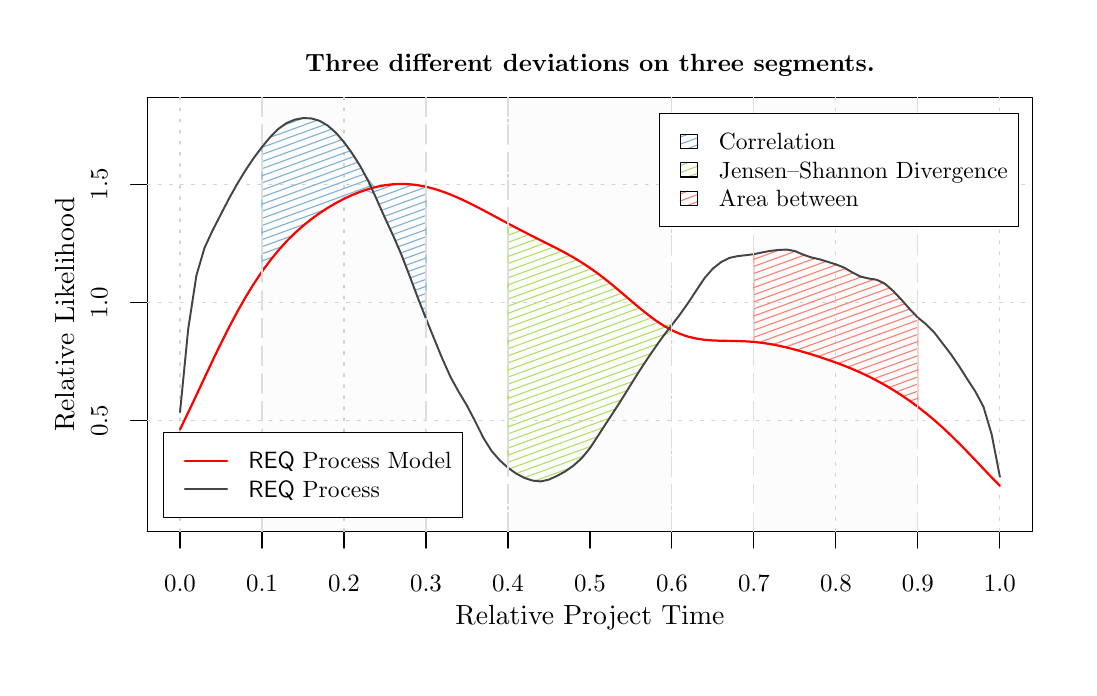
\begin{tikzpicture}[x=1pt,y=1pt]
\definecolor{fillColor}{RGB}{255,255,255}
\path[use as bounding box,fill=fillColor,fill opacity=0.00] (0,0) rectangle (376.36,231.26);
\begin{scope}
\path[clip] (  0.00,  0.00) rectangle (376.36,231.26);
\definecolor{drawColor}{RGB}{0,0,0}

\node[text=drawColor,anchor=base,inner sep=0pt, outer sep=0pt, scale=  0.90] at (203.18,215.56) {\bfseries Three different deviations on three segments.};
\end{scope}
\begin{scope}
\path[clip] (  0.00,  0.00) rectangle (376.36,231.26);
\definecolor{drawColor}{RGB}{0,0,0}

\path[draw=drawColor,line width= 0.4pt,line join=round,line cap=round] ( 55.05, 49.20) -- (351.31, 49.20);

\path[draw=drawColor,line width= 0.4pt,line join=round,line cap=round] ( 55.05, 49.20) -- ( 55.05, 43.20);

\path[draw=drawColor,line width= 0.4pt,line join=round,line cap=round] ( 84.68, 49.20) -- ( 84.68, 43.20);

\path[draw=drawColor,line width= 0.4pt,line join=round,line cap=round] (114.30, 49.20) -- (114.30, 43.20);

\path[draw=drawColor,line width= 0.4pt,line join=round,line cap=round] (143.93, 49.20) -- (143.93, 43.20);

\path[draw=drawColor,line width= 0.4pt,line join=round,line cap=round] (173.55, 49.20) -- (173.55, 43.20);

\path[draw=drawColor,line width= 0.4pt,line join=round,line cap=round] (203.18, 49.20) -- (203.18, 43.20);

\path[draw=drawColor,line width= 0.4pt,line join=round,line cap=round] (232.80, 49.20) -- (232.80, 43.20);

\path[draw=drawColor,line width= 0.4pt,line join=round,line cap=round] (262.43, 49.20) -- (262.43, 43.20);

\path[draw=drawColor,line width= 0.4pt,line join=round,line cap=round] (292.06, 49.20) -- (292.06, 43.20);

\path[draw=drawColor,line width= 0.4pt,line join=round,line cap=round] (321.68, 49.20) -- (321.68, 43.20);

\path[draw=drawColor,line width= 0.4pt,line join=round,line cap=round] (351.31, 49.20) -- (351.31, 43.20);

\node[text=drawColor,anchor=base,inner sep=0pt, outer sep=0pt, scale=  0.90] at ( 55.05, 27.60) {0.0};

\node[text=drawColor,anchor=base,inner sep=0pt, outer sep=0pt, scale=  0.90] at ( 84.68, 27.60) {0.1};

\node[text=drawColor,anchor=base,inner sep=0pt, outer sep=0pt, scale=  0.90] at (114.30, 27.60) {0.2};

\node[text=drawColor,anchor=base,inner sep=0pt, outer sep=0pt, scale=  0.90] at (143.93, 27.60) {0.3};

\node[text=drawColor,anchor=base,inner sep=0pt, outer sep=0pt, scale=  0.90] at (173.55, 27.60) {0.4};

\node[text=drawColor,anchor=base,inner sep=0pt, outer sep=0pt, scale=  0.90] at (203.18, 27.60) {0.5};

\node[text=drawColor,anchor=base,inner sep=0pt, outer sep=0pt, scale=  0.90] at (232.80, 27.60) {0.6};

\node[text=drawColor,anchor=base,inner sep=0pt, outer sep=0pt, scale=  0.90] at (262.43, 27.60) {0.7};

\node[text=drawColor,anchor=base,inner sep=0pt, outer sep=0pt, scale=  0.90] at (292.06, 27.60) {0.8};

\node[text=drawColor,anchor=base,inner sep=0pt, outer sep=0pt, scale=  0.90] at (321.68, 27.60) {0.9};

\node[text=drawColor,anchor=base,inner sep=0pt, outer sep=0pt, scale=  0.90] at (351.31, 27.60) {1.0};

\path[draw=drawColor,line width= 0.4pt,line join=round,line cap=round] ( 43.20, 89.18) -- ( 43.20,174.62);

\path[draw=drawColor,line width= 0.4pt,line join=round,line cap=round] ( 43.20, 89.18) -- ( 37.20, 89.18);

\path[draw=drawColor,line width= 0.4pt,line join=round,line cap=round] ( 43.20,131.90) -- ( 37.20,131.90);

\path[draw=drawColor,line width= 0.4pt,line join=round,line cap=round] ( 43.20,174.62) -- ( 37.20,174.62);

\node[text=drawColor,rotate= 90.00,anchor=base,inner sep=0pt, outer sep=0pt, scale=  0.90] at ( 28.80, 89.18) {0.5};

\node[text=drawColor,rotate= 90.00,anchor=base,inner sep=0pt, outer sep=0pt, scale=  0.90] at ( 28.80,131.90) {1.0};

\node[text=drawColor,rotate= 90.00,anchor=base,inner sep=0pt, outer sep=0pt, scale=  0.90] at ( 28.80,174.62) {1.5};

\node[text=drawColor,anchor=base,inner sep=0pt, outer sep=0pt, scale=  1.00] at (203.18, 15.60) {Relative Project Time};

\node[text=drawColor,rotate= 90.00,anchor=base,inner sep=0pt, outer sep=0pt, scale=  1.00] at ( 16.80,127.63) {Relative Likelihood};

\path[draw=drawColor,line width= 0.4pt,line join=round,line cap=round] ( 43.20, 49.20) --
	(363.16, 49.20) --
	(363.16,206.06) --
	( 43.20,206.06) --
	( 43.20, 49.20);
\end{scope}
\begin{scope}
\path[clip] ( 43.20, 49.20) rectangle (363.16,206.06);
\definecolor{drawColor}{RGB}{211,211,211}

\path[draw=drawColor,line width= 0.4pt,dash pattern=on 1pt off 3pt ,line join=round,line cap=round] ( 55.05, 49.20) -- ( 55.05,206.06);

\path[draw=drawColor,line width= 0.4pt,dash pattern=on 1pt off 3pt ,line join=round,line cap=round] (114.30, 49.20) -- (114.30,206.06);

\path[draw=drawColor,line width= 0.4pt,dash pattern=on 1pt off 3pt ,line join=round,line cap=round] (173.55, 49.20) -- (173.55,206.06);

\path[draw=drawColor,line width= 0.4pt,dash pattern=on 1pt off 3pt ,line join=round,line cap=round] (232.80, 49.20) -- (232.80,206.06);

\path[draw=drawColor,line width= 0.4pt,dash pattern=on 1pt off 3pt ,line join=round,line cap=round] (292.06, 49.20) -- (292.06,206.06);

\path[draw=drawColor,line width= 0.4pt,dash pattern=on 1pt off 3pt ,line join=round,line cap=round] (351.31, 49.20) -- (351.31,206.06);

\path[draw=drawColor,line width= 0.4pt,dash pattern=on 1pt off 3pt ,line join=round,line cap=round] ( 43.20, 89.18) -- (363.16, 89.18);

\path[draw=drawColor,line width= 0.4pt,dash pattern=on 1pt off 3pt ,line join=round,line cap=round] ( 43.20,131.90) -- (363.16,131.90);

\path[draw=drawColor,line width= 0.4pt,dash pattern=on 1pt off 3pt ,line join=round,line cap=round] ( 43.20,174.62) -- (363.16,174.62);
\definecolor{fillColor}{RGB}{0,0,0}

\path[fill=fillColor,fill opacity=0.01] (262.43, 46.47) rectangle (321.68,302.78);
\definecolor{drawColor}{RGB}{251,128,114}

\path[draw=drawColor,line width= 0.4pt,line join=round,line cap=round] (321.16, 94.61) -- (321.68, 94.80);

\path[draw=drawColor,line width= 0.4pt,line join=round,line cap=round] (318.81, 96.32) -- (321.68, 97.37);

\path[draw=drawColor,line width= 0.4pt,line join=round,line cap=round] (316.37, 98.00) -- (321.68, 99.93);

\path[draw=drawColor,line width= 0.4pt,line join=round,line cap=round] (313.84, 99.64) -- (321.68,102.49);

\path[draw=drawColor,line width= 0.4pt,line join=round,line cap=round] (311.21,101.25) -- (321.68,105.06);

\path[draw=drawColor,line width= 0.4pt,line join=round,line cap=round] (308.48,102.82) -- (321.68,107.62);

\path[draw=drawColor,line width= 0.4pt,line join=round,line cap=round] (305.63,104.34) -- (321.68,110.18);

\path[draw=drawColor,line width= 0.4pt,line join=round,line cap=round] (302.65,105.82) -- (321.68,112.75);

\path[draw=drawColor,line width= 0.4pt,line join=round,line cap=round] (299.52,107.25) -- (321.68,115.31);

\path[draw=drawColor,line width= 0.4pt,line join=round,line cap=round] (296.25,108.62) -- (321.68,117.88);

\path[draw=drawColor,line width= 0.4pt,line join=round,line cap=round] (292.84,109.94) -- (321.68,120.44);

\path[draw=drawColor,line width= 0.4pt,line join=round,line cap=round] (289.29,111.21) -- (321.68,123.00);

\path[draw=drawColor,line width= 0.4pt,line join=round,line cap=round] (285.61,112.44) -- (321.68,125.57);

\path[draw=drawColor,line width= 0.4pt,line join=round,line cap=round] (281.82,113.62) -- (320.52,127.71);

\path[draw=drawColor,line width= 0.4pt,line join=round,line cap=round] (277.89,114.75) -- (318.69,129.61);

\path[draw=drawColor,line width= 0.4pt,line join=round,line cap=round] (273.74,115.81) -- (316.97,131.54);

\path[draw=drawColor,line width= 0.4pt,line join=round,line cap=round] (269.29,116.75) -- (315.25,133.48);

\path[draw=drawColor,line width= 0.4pt,line join=round,line cap=round] (264.29,117.50) -- (313.43,135.38);

\path[draw=drawColor,line width= 0.4pt,line join=round,line cap=round] (262.43,119.38) -- (311.48,137.23);

\path[draw=drawColor,line width= 0.4pt,line join=round,line cap=round] (262.43,121.95) -- (309.33,139.02);

\path[draw=drawColor,line width= 0.4pt,line join=round,line cap=round] (262.43,124.51) -- (305.94,140.35);

\path[draw=drawColor,line width= 0.4pt,line join=round,line cap=round] (262.43,127.07) -- (301.43,141.27);

\path[draw=drawColor,line width= 0.4pt,line join=round,line cap=round] (262.43,129.64) -- (298.29,142.69);

\path[draw=drawColor,line width= 0.4pt,line join=round,line cap=round] (262.43,132.20) -- (295.48,144.23);

\path[draw=drawColor,line width= 0.4pt,line join=round,line cap=round] (262.43,134.76) -- (292.26,145.62);

\path[draw=drawColor,line width= 0.4pt,line join=round,line cap=round] (262.43,137.33) -- (288.54,146.83);

\path[draw=drawColor,line width= 0.4pt,line join=round,line cap=round] (262.43,139.89) -- (284.51,147.93);

\path[draw=drawColor,line width= 0.4pt,line join=round,line cap=round] (262.43,142.45) -- (280.64,149.08);

\path[draw=drawColor,line width= 0.4pt,line join=round,line cap=round] (262.43,145.02) -- (277.30,150.43);

\path[draw=drawColor,line width= 0.4pt,line join=round,line cap=round] (262.43,147.58) -- (271.71,150.96);

\path[draw=drawColor,line width= 0.4pt,line join=round,line cap=round] (262.43,149.42) --
	(265.55,150.08) --
	(268.67,150.65) --
	(271.79,150.97) --
	(274.90,151.05) --
	(278.02,150.24) --
	(281.14,148.86) --
	(284.26,147.99) --
	(287.38,147.21) --
	(290.50,146.20) --
	(293.62,145.18) --
	(296.73,143.59) --
	(299.85,141.79) --
	(302.97,140.76) --
	(306.09,140.32) --
	(309.21,139.11) --
	(312.33,136.53) --
	(315.44,133.28) --
	(318.56,129.74) --
	(321.68,126.50) --
	(321.68, 94.23) --
	(318.56, 96.51) --
	(315.44, 98.63) --
	(312.33,100.60) --
	(309.21,102.42) --
	(306.09,104.11) --
	(302.97,105.67) --
	(299.85,107.11) --
	(296.73,108.43) --
	(293.62,109.66) --
	(290.50,110.80) --
	(287.38,111.87) --
	(284.26,112.88) --
	(281.14,113.83) --
	(278.02,114.72) --
	(274.90,115.54) --
	(271.79,116.26) --
	(268.67,116.87) --
	(265.55,117.36) --
	(262.43,117.70) --
	(262.43,149.42);

\path[fill=fillColor,fill opacity=0.01] ( 84.68, 46.47) rectangle (143.93,302.78);
\definecolor{drawColor}{RGB}{128,177,211}

\path[draw=drawColor,line width= 0.4pt,line join=round,line cap=round] (143.44,127.35) -- (143.93,127.52);

\path[draw=drawColor,line width= 0.4pt,line join=round,line cap=round] (142.57,129.59) -- (143.93,130.09);

\path[draw=drawColor,line width= 0.4pt,line join=round,line cap=round] (141.69,131.84) -- (143.93,132.65);

\path[draw=drawColor,line width= 0.4pt,line join=round,line cap=round] (140.82,134.08) -- (143.93,135.21);

\path[draw=drawColor,line width= 0.4pt,line join=round,line cap=round] (139.97,136.34) -- (143.93,137.78);

\path[draw=drawColor,line width= 0.4pt,line join=round,line cap=round] (139.13,138.59) -- (143.93,140.34);

\path[draw=drawColor,line width= 0.4pt,line join=round,line cap=round] (138.28,140.85) -- (143.93,142.90);

\path[draw=drawColor,line width= 0.4pt,line join=round,line cap=round] (137.42,143.10) -- (143.93,145.47);

\path[draw=drawColor,line width= 0.4pt,line join=round,line cap=round] (136.55,145.35) -- (143.93,148.03);

\path[draw=drawColor,line width= 0.4pt,line join=round,line cap=round] (135.67,147.59) -- (143.93,150.60);

\path[draw=drawColor,line width= 0.4pt,line join=round,line cap=round] (134.79,149.83) -- (143.93,153.16);

\path[draw=drawColor,line width= 0.4pt,line join=round,line cap=round] (133.84,152.05) -- (143.93,155.72);

\path[draw=drawColor,line width= 0.4pt,line join=round,line cap=round] (132.86,154.26) -- (143.93,158.29);

\path[draw=drawColor,line width= 0.4pt,line join=round,line cap=round] (131.88,156.46) -- (143.93,160.85);

\path[draw=drawColor,line width= 0.4pt,line join=round,line cap=round] (130.88,158.67) -- (143.93,163.41);

\path[draw=drawColor,line width= 0.4pt,line join=round,line cap=round] ( 84.68,144.41) -- ( 85.97,144.88);

\path[draw=drawColor,line width= 0.4pt,line join=round,line cap=round] (129.87,160.86) -- (143.93,165.98);

\path[draw=drawColor,line width= 0.4pt,line join=round,line cap=round] ( 84.68,146.98) -- ( 88.69,148.43);

\path[draw=drawColor,line width= 0.4pt,line join=round,line cap=round] (128.86,163.06) -- (143.93,168.54);

\path[draw=drawColor,line width= 0.4pt,line join=round,line cap=round] ( 84.68,149.54) -- ( 91.82,152.14);

\path[draw=drawColor,line width= 0.4pt,line join=round,line cap=round] (127.87,165.26) -- (143.93,171.10);

\path[draw=drawColor,line width= 0.4pt,line join=round,line cap=round] ( 84.68,152.10) -- ( 95.60,156.08);

\path[draw=drawColor,line width= 0.4pt,line join=round,line cap=round] (126.89,167.47) -- (143.93,173.67);

\path[draw=drawColor,line width= 0.4pt,line join=round,line cap=round] ( 84.68,154.67) -- (100.36,160.37);

\path[draw=drawColor,line width= 0.4pt,line join=round,line cap=round] (125.91,169.67) -- (139.26,174.53);

\path[draw=drawColor,line width= 0.4pt,line join=round,line cap=round] ( 84.68,157.23) -- (107.48,165.53);

\path[draw=drawColor,line width= 0.4pt,line join=round,line cap=round] (124.30,171.65) -- (132.65,174.69);

\path[draw=drawColor,line width= 0.4pt,line join=round,line cap=round] ( 84.68,159.79) -- (124.63,174.33);

\path[draw=drawColor,line width= 0.4pt,line join=round,line cap=round] ( 84.68,162.36) -- (123.13,176.35);

\path[draw=drawColor,line width= 0.4pt,line join=round,line cap=round] ( 84.68,164.92) -- (121.73,178.41);

\path[draw=drawColor,line width= 0.4pt,line join=round,line cap=round] ( 84.68,167.48) -- (120.51,180.53);

\path[draw=drawColor,line width= 0.4pt,line join=round,line cap=round] ( 84.68,170.05) -- (119.30,182.65);

\path[draw=drawColor,line width= 0.4pt,line join=round,line cap=round] ( 84.68,172.61) -- (117.95,184.72);

\path[draw=drawColor,line width= 0.4pt,line join=round,line cap=round] ( 84.68,175.17) -- (116.57,186.78);

\path[draw=drawColor,line width= 0.4pt,line join=round,line cap=round] ( 84.68,177.74) -- (115.09,188.81);

\path[draw=drawColor,line width= 0.4pt,line join=round,line cap=round] ( 84.68,180.30) -- (113.53,190.80);

\path[draw=drawColor,line width= 0.4pt,line join=round,line cap=round] ( 84.68,182.87) -- (111.81,192.74);

\path[draw=drawColor,line width= 0.4pt,line join=round,line cap=round] ( 84.68,185.43) -- (109.94,194.62);

\path[draw=drawColor,line width= 0.4pt,line join=round,line cap=round] ( 84.68,187.99) -- (107.60,196.34);

\path[draw=drawColor,line width= 0.4pt,line join=round,line cap=round] ( 87.57,191.61) -- (104.63,197.82);

\path[draw=drawColor,line width= 0.4pt,line join=round,line cap=round] ( 92.35,195.91) -- ( 99.55,198.53);

\path[draw=drawColor,line width= 0.4pt,line join=round,line cap=round] ( 84.68,188.16) --
	( 87.79,191.88) --
	( 90.91,194.95) --
	( 94.03,197.04) --
	( 97.15,198.21) --
	(100.27,198.63) --
	(103.39,198.30) --
	(106.51,197.10) --
	(109.62,194.94) --
	(112.74,191.80) --
	(115.86,187.83) --
	(118.98,183.20) --
	(122.10,177.76) --
	(125.22,173.54) --
	(128.33,174.21) --
	(131.45,174.63) --
	(134.57,174.79) --
	(137.69,174.71) --
	(140.81,174.36) --
	(143.93,173.78) --
	(143.93,126.10) --
	(140.81,134.11) --
	(137.69,142.42) --
	(134.57,150.39) --
	(131.45,157.43) --
	(128.33,164.20) --
	(125.22,171.24) --
	(122.10,172.63) --
	(118.98,171.50) --
	(115.86,170.16) --
	(112.74,168.62) --
	(109.62,166.87) --
	(106.51,164.92) --
	(103.39,162.74) --
	(100.27,160.30) --
	( 97.15,157.59) --
	( 94.03,154.55) --
	( 90.91,151.15) --
	( 87.79,147.35) --
	( 84.68,143.13) --
	( 84.68,188.16);

\path[fill=fillColor,fill opacity=0.01] (173.55, 46.47) rectangle (232.80,302.78);
\definecolor{drawColor}{RGB}{179,222,105}

\path[draw=drawColor,line width= 0.4pt,line join=round,line cap=round] (183.24, 67.49) -- (196.03, 72.14);

\path[draw=drawColor,line width= 0.4pt,line join=round,line cap=round] (179.39, 68.65) -- (200.79, 76.44);

\path[draw=drawColor,line width= 0.4pt,line join=round,line cap=round] (176.50, 70.16) -- (203.57, 80.02);

\path[draw=drawColor,line width= 0.4pt,line join=round,line cap=round] (174.11, 71.86) -- (205.87, 83.42);

\path[draw=drawColor,line width= 0.4pt,line join=round,line cap=round] (173.55, 74.22) -- (208.01, 86.76);

\path[draw=drawColor,line width= 0.4pt,line join=round,line cap=round] (173.55, 76.78) -- (210.23, 90.13);

\path[draw=drawColor,line width= 0.4pt,line join=round,line cap=round] (173.55, 79.34) -- (212.42, 93.49);

\path[draw=drawColor,line width= 0.4pt,line join=round,line cap=round] (173.55, 81.91) -- (214.57, 96.84);

\path[draw=drawColor,line width= 0.4pt,line join=round,line cap=round] (173.55, 84.47) -- (216.63,100.15);

\path[draw=drawColor,line width= 0.4pt,line join=round,line cap=round] (173.55, 87.03) -- (218.69,103.46);

\path[draw=drawColor,line width= 0.4pt,line join=round,line cap=round] (173.55, 89.60) -- (220.78,106.79);

\path[draw=drawColor,line width= 0.4pt,line join=round,line cap=round] (173.55, 92.16) -- (222.97,110.15);

\path[draw=drawColor,line width= 0.4pt,line join=round,line cap=round] (173.55, 94.72) -- (225.26,113.55);

\path[draw=drawColor,line width= 0.4pt,line join=round,line cap=round] (173.55, 97.29) -- (227.65,116.98);

\path[draw=drawColor,line width= 0.4pt,line join=round,line cap=round] (173.55, 99.85) -- (231.18,120.82);

\path[draw=drawColor,line width= 0.4pt,line join=round,line cap=round] (173.55,102.42) -- (232.38,123.83);

\path[draw=drawColor,line width= 0.4pt,line join=round,line cap=round] (173.55,104.98) -- (227.98,124.79);

\path[draw=drawColor,line width= 0.4pt,line join=round,line cap=round] (173.55,107.54) -- (225.57,126.48);

\path[draw=drawColor,line width= 0.4pt,line join=round,line cap=round] (173.55,110.11) -- (223.28,128.21);

\path[draw=drawColor,line width= 0.4pt,line join=round,line cap=round] (173.55,112.67) -- (221.11,129.98);

\path[draw=drawColor,line width= 0.4pt,line join=round,line cap=round] (173.55,115.23) -- (218.98,131.77);

\path[draw=drawColor,line width= 0.4pt,line join=round,line cap=round] (173.55,117.80) -- (216.87,133.56);

\path[draw=drawColor,line width= 0.4pt,line join=round,line cap=round] (173.55,120.36) -- (214.77,135.36);

\path[draw=drawColor,line width= 0.4pt,line join=round,line cap=round] (173.55,122.92) -- (212.64,137.15);

\path[draw=drawColor,line width= 0.4pt,line join=round,line cap=round] (173.55,125.49) -- (210.49,138.93);

\path[draw=drawColor,line width= 0.4pt,line join=round,line cap=round] (173.55,128.05) -- (208.29,140.69);

\path[draw=drawColor,line width= 0.4pt,line join=round,line cap=round] (173.55,130.62) -- (206.00,142.42);

\path[draw=drawColor,line width= 0.4pt,line join=round,line cap=round] (173.55,133.18) -- (203.62,144.12);

\path[draw=drawColor,line width= 0.4pt,line join=round,line cap=round] (173.55,135.74) -- (201.16,145.79);

\path[draw=drawColor,line width= 0.4pt,line join=round,line cap=round] (173.55,138.31) -- (198.58,147.41);

\path[draw=drawColor,line width= 0.4pt,line join=round,line cap=round] (173.55,140.87) -- (195.86,148.99);

\path[draw=drawColor,line width= 0.4pt,line join=round,line cap=round] (173.55,143.43) -- (193.05,150.53);

\path[draw=drawColor,line width= 0.4pt,line join=round,line cap=round] (173.55,146.00) -- (190.15,152.04);

\path[draw=drawColor,line width= 0.4pt,line join=round,line cap=round] (173.55,148.56) -- (187.20,153.53);

\path[draw=drawColor,line width= 0.4pt,line join=round,line cap=round] (173.55,151.12) -- (184.23,155.01);

\path[draw=drawColor,line width= 0.4pt,line join=round,line cap=round] (173.55,153.69) -- (181.27,156.50);

\path[draw=drawColor,line width= 0.4pt,line join=round,line cap=round] (173.55,156.25) -- (178.35,158.00);

\path[draw=drawColor,line width= 0.4pt,line join=round,line cap=round] (173.55,158.81) -- (175.45,159.51);

\path[draw=drawColor,line width= 0.4pt,line join=round,line cap=round] (173.55,160.51) --
	(176.67,158.86) --
	(179.79,157.25) --
	(182.91,155.67) --
	(186.03,154.11) --
	(189.15,152.55) --
	(192.26,150.95) --
	(195.38,149.27) --
	(198.50,147.46) --
	(201.62,145.50) --
	(204.74,143.36) --
	(207.86,141.04) --
	(210.98,138.55) --
	(214.09,135.94) --
	(217.21,133.27) --
	(220.33,130.62) --
	(223.45,128.07) --
	(226.57,125.72) --
	(229.69,123.65) --
	(232.80,123.85) --
	(232.80,121.90) --
	(229.69,119.84) --
	(226.57,115.46) --
	(223.45,110.88) --
	(220.33,106.10) --
	(217.21,101.09) --
	(214.09, 96.07) --
	(210.98, 91.26) --
	(207.86, 86.52) --
	(204.74, 81.64) --
	(201.62, 77.30) --
	(198.50, 74.08) --
	(195.38, 71.63) --
	(192.26, 69.80) --
	(189.15, 68.27) --
	(186.03, 67.35) --
	(182.91, 67.50) --
	(179.79, 68.45) --
	(176.67, 70.04) --
	(173.55, 72.25) --
	(173.55,160.51);
\definecolor{drawColor}{RGB}{255,0,0}

\path[draw=drawColor,line width= 0.8pt,line join=round,line cap=round] ( 55.05, 86.09) --
	( 58.01, 92.21) --
	( 60.98, 98.49) --
	( 63.94,104.83) --
	( 66.90,111.11) --
	( 69.86,117.23) --
	( 72.83,123.11) --
	( 75.79,128.68) --
	( 78.75,133.88) --
	( 81.71,138.71) --
	( 84.68,143.13) --
	( 87.64,147.15) --
	( 90.60,150.78) --
	( 93.56,154.06) --
	( 96.53,157.01) --
	( 99.49,159.65) --
	(102.45,162.04) --
	(105.41,164.18) --
	(108.38,166.12) --
	(111.34,167.86) --
	(114.30,169.42) --
	(117.26,170.79) --
	(120.23,171.98) --
	(123.19,172.97) --
	(126.15,173.76) --
	(129.11,174.34) --
	(132.08,174.68) --
	(135.04,174.80) --
	(138.00,174.68) --
	(140.96,174.34) --
	(143.93,173.78) --
	(146.89,173.02) --
	(149.85,172.07) --
	(152.82,170.95) --
	(155.78,169.68) --
	(158.74,168.30) --
	(161.70,166.83) --
	(164.67,165.28) --
	(167.63,163.70) --
	(170.59,162.10) --
	(173.55,160.51) --
	(176.52,158.94) --
	(179.48,157.41) --
	(182.44,155.91) --
	(185.40,154.43) --
	(188.37,152.94) --
	(191.33,151.44) --
	(194.29,149.87) --
	(197.25,148.20) --
	(200.22,146.40) --
	(203.18,144.45) --
	(206.14,142.34) --
	(209.10,140.06) --
	(212.07,137.65) --
	(215.03,135.14) --
	(217.99,132.60) --
	(220.95,130.10) --
	(223.92,127.71) --
	(226.88,125.50) --
	(229.84,123.55) --
	(232.80,121.90) --
	(235.77,120.58) --
	(238.73,119.59) --
	(241.69,118.90) --
	(244.65,118.46) --
	(247.62,118.23) --
	(250.58,118.12) --
	(253.54,118.08) --
	(256.51,118.02) --
	(259.47,117.91) --
	(262.43,117.70) --
	(265.39,117.38) --
	(268.36,116.93) --
	(271.32,116.36) --
	(274.28,115.69) --
	(277.24,114.93) --
	(280.21,114.10) --
	(283.17,113.22) --
	(286.13,112.28) --
	(289.09,111.29) --
	(292.06,110.24) --
	(295.02,109.12) --
	(297.98,107.91) --
	(300.94,106.62) --
	(303.91,105.22) --
	(306.87,103.70) --
	(309.83,102.07) --
	(312.79,100.31) --
	(315.76, 98.42) --
	(318.72, 96.40) --
	(321.68, 94.23) --
	(324.64, 91.91) --
	(327.61, 89.44) --
	(330.57, 86.81) --
	(333.53, 84.03) --
	(336.49, 81.12) --
	(339.46, 78.09) --
	(342.42, 74.99) --
	(345.38, 71.86) --
	(348.34, 68.75) --
	(351.31, 65.73);
\definecolor{drawColor}{RGB}{68,68,68}

\path[draw=drawColor,line width= 0.7pt,line join=round,line cap=round] ( 55.05, 92.30) --
	( 58.01,122.40) --
	( 60.98,141.78) --
	( 63.94,151.79) --
	( 66.90,158.16) --
	( 69.86,163.92) --
	( 72.83,169.64) --
	( 75.79,174.95) --
	( 78.75,179.77) --
	( 81.71,184.20) --
	( 84.68,188.16) --
	( 87.64,191.71) --
	( 90.60,194.69) --
	( 93.56,196.79) --
	( 96.53,198.04) --
	( 99.49,198.59) --
	(102.45,198.48) --
	(105.41,197.63) --
	(108.38,195.92) --
	(111.34,193.33) --
	(114.30,189.90) --
	(117.26,185.83) --
	(120.23,181.14) --
	(123.19,175.59) --
	(126.15,169.14) --
	(129.11,162.48) --
	(132.08,156.08) --
	(135.04,149.25) --
	(138.00,141.59) --
	(140.96,133.70) --
	(143.93,126.10) --
	(146.89,118.81) --
	(149.85,111.60) --
	(152.82,104.99) --
	(155.78, 99.61) --
	(158.74, 94.68) --
	(161.70, 89.01) --
	(164.67, 83.03) --
	(167.63, 78.31) --
	(170.59, 74.93) --
	(173.55, 72.25) --
	(176.52, 70.13) --
	(179.48, 68.58) --
	(182.44, 67.60) --
	(185.40, 67.29) --
	(188.37, 67.96) --
	(191.33, 69.32) --
	(194.29, 70.94) --
	(197.25, 73.02) --
	(200.22, 75.72) --
	(203.18, 79.33) --
	(206.14, 83.83) --
	(209.10, 88.44) --
	(212.07, 92.92) --
	(215.03, 97.56) --
	(217.99,102.35) --
	(220.95,107.08) --
	(223.92,111.57) --
	(226.88,115.91) --
	(229.84,120.05) --
	(232.80,123.85) --
	(235.77,127.72) --
	(238.73,131.92) --
	(241.69,136.43) --
	(244.65,140.84) --
	(247.62,144.23) --
	(250.58,146.56) --
	(253.54,148.06) --
	(256.51,148.70) --
	(259.47,149.04) --
	(262.43,149.42) --
	(265.39,150.04) --
	(268.36,150.61) --
	(271.32,150.93) --
	(274.28,151.08) --
	(277.24,150.54) --
	(280.21,149.25) --
	(283.17,148.23) --
	(286.13,147.57) --
	(289.09,146.65) --
	(292.06,145.72) --
	(295.02,144.55) --
	(297.98,142.83) --
	(300.94,141.31) --
	(303.91,140.62) --
	(306.87,140.15) --
	(309.83,138.69) --
	(312.79,136.06) --
	(315.76,132.94) --
	(318.72,129.56) --
	(321.68,126.50) --
	(324.64,124.09) --
	(327.61,121.08) --
	(330.57,117.23) --
	(333.53,113.36) --
	(336.49,109.06) --
	(339.46,104.36) --
	(342.42, 99.82) --
	(345.38, 94.26) --
	(348.34, 84.27) --
	(351.31, 68.95);
\definecolor{drawColor}{RGB}{221,221,221}

\path[draw=drawColor,line width= 0.4pt,dash pattern=on 7pt off 3pt ,line join=round,line cap=round] ( 84.68, 49.20) -- ( 84.68,206.06);

\path[draw=drawColor,line width= 0.4pt,dash pattern=on 7pt off 3pt ,line join=round,line cap=round] (143.93, 49.20) -- (143.93,206.06);

\path[draw=drawColor,line width= 0.4pt,dash pattern=on 7pt off 3pt ,line join=round,line cap=round] (173.55, 49.20) -- (173.55,206.06);

\path[draw=drawColor,line width= 0.4pt,dash pattern=on 7pt off 3pt ,line join=round,line cap=round] (232.80, 49.20) -- (232.80,206.06);

\path[draw=drawColor,line width= 0.4pt,dash pattern=on 7pt off 3pt ,line join=round,line cap=round] (262.43, 49.20) -- (262.43,206.06);

\path[draw=drawColor,line width= 0.4pt,dash pattern=on 7pt off 3pt ,line join=round,line cap=round] (321.68, 49.20) -- (321.68,206.06);
\definecolor{drawColor}{RGB}{0,0,0}
\definecolor{fillColor}{RGB}{255,255,255}

\path[draw=drawColor,line width= 0.4pt,line join=round,line cap=round,fill=fillColor] (228.36,200.25) rectangle (358.01,159.45);
\definecolor{drawColor}{RGB}{128,177,211}

\path[draw=drawColor,line width= 0.4pt,line join=round,line cap=round] (238.29,187.50) -- (242.13,188.90);

\path[draw=drawColor,line width= 0.4pt,line join=round,line cap=round] (236.01,189.24) -- (242.13,191.47);

\path[draw=drawColor,line width= 0.4pt,line join=round,line cap=round] (236.01,191.80) -- (238.21,192.60);
\definecolor{drawColor}{RGB}{179,222,105}

\path[draw=drawColor,line width= 0.4pt,line join=round,line cap=round] (238.44,177.30) -- (242.13,178.65);

\path[draw=drawColor,line width= 0.4pt,line join=round,line cap=round] (236.01,178.98) -- (242.13,181.21);

\path[draw=drawColor,line width= 0.4pt,line join=round,line cap=round] (236.01,181.55) -- (238.36,182.40);
\definecolor{drawColor}{RGB}{251,128,114}

\path[draw=drawColor,line width= 0.4pt,line join=round,line cap=round] (238.59,167.10) -- (242.13,168.39);

\path[draw=drawColor,line width= 0.4pt,line join=round,line cap=round] (236.01,168.73) -- (242.13,170.96);

\path[draw=drawColor,line width= 0.4pt,line join=round,line cap=round] (236.01,171.29) -- (238.51,172.20);
\definecolor{drawColor}{RGB}{0,0,0}

\path[draw=drawColor,line width= 0.4pt,line join=round,line cap=round] (236.01,192.60) --
	(242.13,192.60) --
	(242.13,187.50) --
	(236.01,187.50) --
	(236.01,192.60);

\path[draw=drawColor,line width= 0.4pt,line join=round,line cap=round] (236.01,182.40) --
	(242.13,182.40) --
	(242.13,177.30) --
	(236.01,177.30) --
	(236.01,182.40);

\path[draw=drawColor,line width= 0.4pt,line join=round,line cap=round] (236.01,172.20) --
	(242.13,172.20) --
	(242.13,167.10) --
	(236.01,167.10) --
	(236.01,172.20);

\node[text=drawColor,anchor=base west,inner sep=0pt, outer sep=0pt, scale=  0.85] at (249.78,187.13) {Correlation};

\node[text=drawColor,anchor=base west,inner sep=0pt, outer sep=0pt, scale=  0.85] at (249.78,176.93) {Jensen--Shannon Divergence};

\node[text=drawColor,anchor=base west,inner sep=0pt, outer sep=0pt, scale=  0.85] at (249.78,166.73) {Area between};

\path[draw=drawColor,line width= 0.4pt,line join=round,line cap=round,fill=fillColor] ( 49.13, 84.91) rectangle (157.02, 54.31);
\definecolor{drawColor}{RGB}{255,0,0}

\path[draw=drawColor,line width= 0.8pt,line join=round,line cap=round] ( 56.78, 74.71) -- ( 72.08, 74.71);
\definecolor{drawColor}{RGB}{68,68,68}

\path[draw=drawColor,line width= 0.7pt,line join=round,line cap=round] ( 56.78, 64.51) -- ( 72.08, 64.51);
\definecolor{drawColor}{RGB}{0,0,0}

\node[text=drawColor,anchor=base west,inner sep=0pt, outer sep=0pt, scale=  0.85] at ( 79.73, 71.79) {\textsf{REQ} Process Model};

\node[text=drawColor,anchor=base west,inner sep=0pt, outer sep=0pt, scale=  0.85] at ( 79.73, 61.59) {\textsf{REQ} Process};
\end{scope}
\end{tikzpicture}
}
    \caption[Three different deviations between two continuous software processes.]{{\small The deviations between the weighted mixture (red) and a project (black) for the activity \textsf{REQ}.}}
    \label{fig:ac-raw-vs-scores}
\end{figure}


A unit change is equal across any two scores that were previously calibrated using Automatic Calibration.
Therefore, we can also compare the achieved scores even though their underlying quantities are vastly different.
The correlation on the first segment achieved a score of $\utight{\approx}0.28$ out of $1.0$.
This seems reasonable when inspecting Figure~\ref{fig:ac-raw-vs-scores}, where only a smaller portion of the curves has a positive correlation.
The Jensen--Shannon divergence on the second segment scored very low with $\utight{\approx}0.02$.
Given that the two curves on that segment not only behave completely differently but also have a large spatial distance, a large divergence (and hence a low score) appears to be sound.
Lastly, the area in between curves scored $\utight{\approx}0.41$ on the last segment.
We observe a somewhat large area between the curves and this score tells us that more than $40$\% of the other simulated curves' area on that segment is even larger.

The achieved scores can be ordered as $\mathbf{area}>\mathbf{corr}>\mathbf{jsd}$ and their relative importance can be used to calculate an approximate result (total match).
However, only individual scores should be evaluated in order to replace portions of the qualitative evaluation, as a simple aggregation of scores might be misleading as it cannot capture more complex relations and non-linearities between scores and the dependent variable (even a simple aggregation is a kind of regression model, too, and it is likely to be different from the trained model).

When evaluating individual scores in order to find the smallest or largest deviations, we may also use the (scaled) variable importance to produce weighted scores, in order to better understand the outcome of the regression model (see Table~\ref{tab:ac-raw-vs-scores}).
The order for the scaled scores changes to $\mathbf{corr}>\mathbf{area}>\mathbf{jsd}$.
While we still have the lowest score/largest deviation/biggest problem with the divergence in the middle segment, the second-largest problem appears now to be the area between curves in the last segment.
It is these quantitatively derived insights that we suggest can add to the picture of qualitative evaluation.


\cleardoublepage
\chapter{Concluding Remarks and Future Work}\label{chap:conclusions-future-work}%
\vspace{5pt}
\chaptertoc
\chaptermark{Conclusions \& Future work}

\noindent
This chapter concludes the results of the presented publications and discusses their limitations.
This is followed by an outline of prospective future work.

\section{Limitations}


\section{Conclusions}

\section{Future Work}
%



\cleardoublepage


%----------------------------------------------------------------------------------------------------
%---------------------HERE STARTS THE APPENDIX -----------------------------------
%----------------------------------------------------------------------------------------------------


\phantomsection
\addcontentsline{toc}{chapter}{Bibliography}


\renewcommand*{\bibfont}{\small}
\printbibliography
\cleardoublepage



\begin{appendices}
%\appendixpage
\noappendicestocpagenum
\addappheadtotoc



%\renewcommand{\myfullcite}[1]{\printpublication{#1}~\cite{#1}.}
\renewcommand{\myfullcite}[1]{\printpublication{#1}.}



\renewcommand{\appendixname}{Paper}
\chapter{A changeset-based approach to assess source code density and developer efficacy}\label{app:publ-honel2018changeset}
\chaptermark{\label{app:publ-honel2018changeset}}
\myfullcite{honel2018changeset}





\chapter{Importance and Aptitude of Source Code Density for Commit Classification into Maintenance Activities}\label{app:publ-honel19importance}
\chaptermark{\label{app:publ-honel19importance}}
\myfullcite{honel19importance}





\renewcommand{\appendixname}{Article}
\chapter{Using source code density to improve the accuracy of automatic commit classification into maintenance activities}\label{app:publ-honel2020using}
\chaptermark{\label{app:publ-honel2020using}}
\myfullcite{honel2020using}





\renewcommand{\appendixname}{Paper}
\chapter{Exploiting Relations, Sojourn-Times, and Joint Conditional Probabilities for Automated Commit Classification}\label{app:publ-honel2023hmm}
\chaptermark{\label{app:publ-honel2023hmm}}
\myfullcite{honel2023hmm}





\chapter{\texorpdfstring{Process Anti-Pattern Detection\,--\,a Case Study}{Process Anti-Pattern Detection - a Case Study}}\label{app:publ-picha_honel22pilot}
\chaptermark{\label{app:publ-picha_honel22pilot}}
\myfullcite{picha_honel22pilot}





\renewcommand{\appendixname}{Article}
\chapter{Activity-Based Detection of (Anti-)Patterns: An Embedded Case Study of the Fire Drill}\label{app:publ-honel2023embedded}
\chaptermark{\label{app:publ-honel2023embedded}}
\myfullcite{honel2023embedded}





\renewcommand{\appendixname}{Paper}
\chapter{Contextual Operationalization of Metrics as Scores: Is My Metric Value Good?}\label{app:publ-honel2022qrsmas}
\chaptermark{\label{app:publ-honel2022qrsmas}}
\myfullcite{honel2022qrsmas}





\renewcommand{\appendixname}{Article}
\chapter{Metrics As Scores: A Tool- and Analysis Suite and Interactive Application for Exploring Context-Dependent Distributions}\label{app:publ-honel2023masjoss}
\chaptermark{\label{app:publ-honel2023masjoss}}
\myfullcite{honel2023masjoss}






\end{appendices}
\afterpage{\blankpage}
\cleardoublepage


\includepdf[pages=-]{papers/MIT_avhandlingsblad_2023_print.pdf}
\cleardoublepage

\backmatter
\cleardoublepage

\end{document}
